% !TEX root = ../../autoreferat.tex
\ifdefined\CELE
\else
\documentclass[a4paper,12pt]{scrreprt}

\usepackage[utf8]{inputenc}
\usepackage[czech]{babel}
\usepackage[T1]{fontenc}
\usepackage{amsmath}
\usepackage{amsfonts}
\usepackage{amssymb}
\usepackage{graphicx}
\usepackage{longtable}
\author{Jan Bartošek}
\usepackage{cite}
\usepackage{url}
\usepackage{subfig}
\usepackage{multibib}
\usepackage[hidelinks,unicode]{hyperref}

%\usepackage{epsfig}
%\usepackage{epstopdf}

\linespread{1.1}
\usepackage{a4wide}

%\usepackage[raggedright]{titlesec} % zamezeni deleni nadpisu

%\newcites{all}{Seznam literatury}
\newcites{my}{Soupis publikací}

\newcommand*{\tabh}[1]{\multicolumn{1}{|c|}{#1}}

\captionsetup{justification=centering}

\begin{document}

\fi

\chapter{Příčiny ztráty hlasu a možnosti jeho rehabilitace}
\label{chap:cause}

Lidská řeč tvoří jeden ze základních stavebních kamenů lidského dorozumívání. Pro člověka
postiženého ať už dočasnou či trvalou ztrátou hlasu představuje běžná lidská
komunikace mnohem náročnější úkol než pro člověka zdravého. Takový jedinec se
musí dennodenně potýkat s~problémy, které by za normálních okolností řešit
nemusel. To s sebou nese %V mnoha případech doprovází ztrátu hlasu
i zvýšenou psychickou zátěž, nemalý počet pacientů má například obavy %například strach
z~reakce okolí. Proto se problematice rehabilitace jejich
hlasu věnuje nemalá pozornost.
% V~této kapitole jsou nejprve v~části
% \ref{chap:cause:desease} přiblíženy možné příčiny ztráty hlasivek, a tedy i
% trvalé ztráty hlasu, a následně jsou v~části \ref{chap:cause:treatment} představeny
% nejčastěji využívané metody rehabilitace hlasu.

% include other files for sections of this chapter. These use the 'input' command since each section within a chapter should not start a new page.
% If you want to swap the order of sections, it is as simple as reversing the order you include them.
%!TEX root = ../thesis.tex
\section{Příčiny ztráty hlasu}
\label{chap:cause:desease}

Nejčastěji je trvalá ztráta hlasu zapříčiněna chirurgickým zákrokem zvaným
totální laryngektomie\footnote{\textbf{laryngektomie}: larynx, laryngos -
hrtan, ectos, ectomia - odstranění, vynětí} neboli úplné odstranění hrtanu.
Odstraněním hrtanu, a tím i hlasivek (glottis), přichází člověk o~schopnost
rozvibrovat vzduch vycházející z~plic, který je dále modulován artikulačním
ústrojím. Nejběžnější příčinou vedoucí k totální laryngektomii představuje
rakovina hrtanu v~pokročilém stádiu. V~mnohem nižší míře je na vině rakovina
hltanu či poškození hrtanu automobilovou nebo jinou traumatickou nehodou.
Podle \cite{Slavicek2000} přibude v České republice ročně přibližně 400 nových
onemocnění rakoviny hrtanu, z toho je přibližně jedna třetina léčena pomocí
totální laryngektomie. To představuje více než 100 nových případů trvalé
ztráty hlasu každý rok.

\subsection{Rakovina hrtanu} % (fold)
\label{chap:cause:desease:cancer}

Jak již bylo zmíněno, rakovina hrtanu je jedním z hlavních důvodů odstranění
hrtanu. Tento typ rakoviny postihuje převážně muže ve věku 50-60 let.
V~posledních letech je však zřejmý trend snižujícího se průměrného věku
pacientů \cite{Skvrnakova2010}. Z~celkovém počtu pacientů zhruba 20\%
představují ženy.

Přesná příčina vzniku nádorovitého onemocnění hrtanu doposud není známa, ale
z~průzkumů je zřejmá korelace mezi vznikem rakoviny a konzumací alkoholu či
kouřením. Jinými slovy, mezi rizikovou skupinu patří lidé, kteří jsou
pravidelně vystavováni vlivu kouření, ať již aktivně (sami kouří) či pasivně
(vdechují cigaretový kouř) a zároveň si dopřávají nemalé množství alkoholu.
Podle \cite{Skvrnakova2010} 90\% pacientů aktivně kuří.

\subsubsection{Příznaky onemocněni} % (fold)
\label{chap:cause:desease:cancer:symptom}

Vznikající nádorové onemocnění v oblasti hrtanu se může projevovat různými
způsoby. Mezi hlavní faktory ovlivňující počáteční příznaky patří umístění a
velikost nádoru.

Již ve velmi raném stádiu, kdy je nádor umístěn přímo na hlasivkách, je
příznakem \textbf{chrapot}. Ve většině případů se samozřejmě jedná o
krátkodobé postižení hlasivek virovou infekcí. Nicméně pokud chrapot trvá déle
než tři týdny, je již doporučováno navštívit odborného lékaře.
U nádorů nacházejících se ve vchodu do hrtanu a v polykacích cestách se mohou
jako příznak objevovat \textbf{polykací obtíže}. Mezi další možné příznaky
patří \textbf{bolesti v~krku}, jednostranné bolesti vystřelující do ucha čí
nepříjemný pocit při polykání. I~v~tomto případě krátkodobý výskyt nemusí
nutně znamenat rakovinu hrtanu, nicméně při obtížích trvajících déle než měsíc
je doporučováno důkladné  vyšetření lékařem.
Na základě umístění nádoru se může objevovat \textbf{dráždivý kašel} s možným
vykašláváním krve. Dalším možným příznakem je vznik \textbf{zduření na krku}.
V tomto případě je vhodné neprodleně vyhledat lékaře.

Z výše uvedených příznaků je zřejmé, že prvotní indicie o vážném onemocnění
mohou být podceněny, a tím značně snížena šance na plné uzdravení pacienta.
V~případě včasného diagnostikování rakoviny hrtanu či hltanu je možnost
úplného vyléčení pacienta bez trvalých následků více než 90\%
\cite{Slavicek2000}.

% subsubsection příznaky_onemocnění (end)

\subsubsection{Léčba nádorového onemocnění} % (fold)
\label{chap:cause:desease:cancer:treatment}

U nádorovitých onemocnění se v drtivé většině případů využívá
\textbf{chirurgické léčby}, \textbf{aktinoterapie} neboli ozařování a
\textbf{chemoterapie}. Nejinak tomu je i v případě rakoviny hrtanu a
polykacích cest obecně. Majoritní část pacientů je zpravidla nejprve
konfrontována s chirurgickou léčbou. Mezi nejčastější zákroky patří
\textbf{tracheostomie}, parciální laryngektomie, \textbf{totální
laryngektomie} a chordektomie. V~rámci této práce budou blíže popsány pouze
léčebné postupy přímo související s úplným odstraněním hrtanu a hlasivek.

Totální laryngektomie (TL), jak už název napovídá, představuje chirurgický
zákrok, při kterém je úplně odstraněn hrtan. V určitých případech může být
odstraněna i menší či větší část hltanu. Tento zákrok, ve spojení s léčbou
rakoviny hrtanu, poprvé vykonal Dr. Theodor Billroth 31. prosince roku 1873 ve
Vídni \cite{Gussenbauer1874} a do dnešní doby přežil v podstatě nezměněn.
Cílem této operace je odstranění orgánu zasaženého rakovinným bujením, a tedy
zamezení dalšího šíření nemoci. Součástí hrtanu je také hrtanová příklopka
(latinsky epiglottis), která zamezuje vdechnutí potravy nebo tekutin do
dýchacích cest. Po odstranění hrtanu by tedy potrava a tekutiny mohly být
vdechnuty do plic a z tohoto důvodu jsou jícen a průdušnice trvale odděleny.
Rozdíl mezi zdravým člověkem a osobou po totální laryngektomii je znázorněn na
obr. \ref{fig:cause:desease:laryngectomy}.

\begin{figure}[htb]
  \begin{center}
    \def\svgwidth{0.9\linewidth}
    % %LaTeX with PSTricks extensions
%%Creator: 0.48.3.1
%%Please note this file requires PSTricks extensions
\psset{xunit=.5pt,yunit=.5pt,runit=.5pt}
\begin{pspicture}(2907.24389648,1381.22814941)
{
\newrgbcolor{curcolor}{0.9254902 0.9254902 0.9254902}
\pscustom[linestyle=none,fillstyle=solid,fillcolor=curcolor]
{
\newpath
\moveto(70.56024,976.91215941)
\curveto(75.70194,998.05546941)(75.05233,1002.21845941)(63.72468,1022.97718941)
\curveto(59.11246,1029.25078941)(55.53152,1042.76249941)(57.82397,1051.05492941)
\curveto(72.33535,1103.54679941)(151.12483,1181.98458841)(191.6593,1238.29379441)
\curveto(203.82655,1249.22791741)(227.588336,1294.48932741)(288.348581,1301.70009441)
\curveto(395.40091,1303.19005241)(412.940729,1303.02200041)(510.35569,1299.36034741)
\curveto(591.16393,1298.04450341)(563.1446,1253.97868341)(596.12059,1219.46677821)
\curveto(617.11351,1196.64470041)(637.32731,1195.59050941)(673.24323,1168.28753341)
\curveto(683.09539,1161.70729041)(674.18628,1150.76886041)(694.17272,1144.46094641)
\curveto(700.8548,1138.26728041)(689.58524,1131.75588441)(714.56462,1126.38918541)
\curveto(718.47149,1127.09967441)(720.01648,1117.64831941)(721.82813,1108.38187941)
\curveto(742.89519,1091.67695941)(766.01459,1078.47903941)(770.6489,1036.21205941)
\curveto(785.52916,964.13363941)(785.41095,874.88456941)(793.05455,794.70262941)
\curveto(801.16608,725.36812941)(797.04543,665.20049941)(808.62059,580.55167941)
\curveto(817.99398,520.80324941)(824.99343,461.05482941)(838.33757,401.30639941)
\curveto(852.58351,343.43859941)(884.634,245.85682941)(902.96021,169.23090941)
\curveto(920.58527,111.57990941)(928.99355,58.22450941)(939.28097,2.24980941)
\lineto(1191.38979,0.50000941)
\curveto(1147.46289,192.92300941)(1072.39851,239.15118941)(1049.32187,456.03356941)
\curveto(1054.33227,575.87003941)(1066.33852,587.71091941)(1110.16719,692.25659941)
\curveto(1142.86475,756.08452941)(1187.16897,836.01858941)(1215.75173,966.06054941)
\curveto(1241.69732,1053.47858941)(1239.12891,1068.56755941)(1262.28051,1198.70444641)
\curveto(1274.15414,1272.24631941)(1276.84845,1302.56969941)(1275.20381,1380.20462941)
\curveto(1243.6598,1381.01350941)(132.01823,1379.13434941)(108.97269,1379.62040941)
\curveto(89.62734,1380.02842941)(136.091,1338.49754941)(140.67855,1310.22027841)
\curveto(145.31215,1281.65916741)(141.36641,1284.78090841)(130.36263,1262.73876141)
\curveto(114.38301,1230.72928461)(103.72405,1212.44353221)(84.57988,1181.51309641)
\curveto(46.3326,1119.71856941)(3.13314,1081.66825941)(0.88674,1049.70937941)
\curveto(-3.93696,981.08423941)(37.32565,977.54602941)(70.95213,976.84547941)
}
}
{
\newrgbcolor{curcolor}{0 0 0}
\pscustom[linewidth=1,linecolor=curcolor]
{
\newpath
\moveto(70.56024,976.91215941)
\curveto(75.70194,998.05546941)(75.05233,1002.21845941)(63.72468,1022.97718941)
\curveto(59.11246,1029.25078941)(55.53152,1042.76249941)(57.82397,1051.05492941)
\curveto(72.33535,1103.54679941)(151.12483,1181.98458841)(191.6593,1238.29379441)
\curveto(203.82655,1249.22791741)(227.588336,1294.48932741)(288.348581,1301.70009441)
\curveto(395.40091,1303.19005241)(412.940729,1303.02200041)(510.35569,1299.36034741)
\curveto(591.16393,1298.04450341)(563.1446,1253.97868341)(596.12059,1219.46677821)
\curveto(617.11351,1196.64470041)(637.32731,1195.59050941)(673.24323,1168.28753341)
\curveto(683.09539,1161.70729041)(674.18628,1150.76886041)(694.17272,1144.46094641)
\curveto(700.8548,1138.26728041)(689.58524,1131.75588441)(714.56462,1126.38918541)
\curveto(718.47149,1127.09967441)(720.01648,1117.64831941)(721.82813,1108.38187941)
\curveto(742.89519,1091.67695941)(766.01459,1078.47903941)(770.6489,1036.21205941)
\curveto(785.52916,964.13363941)(785.41095,874.88456941)(793.05455,794.70262941)
\curveto(801.16608,725.36812941)(797.04543,665.20049941)(808.62059,580.55167941)
\curveto(817.99398,520.80324941)(824.99343,461.05482941)(838.33757,401.30639941)
\curveto(852.58351,343.43859941)(884.634,245.85682941)(902.96021,169.23090941)
\curveto(920.58527,111.57990941)(928.99355,58.22450941)(939.28097,2.24980941)
\lineto(1191.38979,0.50000941)
\curveto(1147.46289,192.92300941)(1072.39851,239.15118941)(1049.32187,456.03356941)
\curveto(1054.33227,575.87003941)(1066.33852,587.71091941)(1110.16719,692.25659941)
\curveto(1142.86475,756.08452941)(1187.16897,836.01858941)(1215.75173,966.06054941)
\curveto(1241.69732,1053.47858941)(1239.12891,1068.56755941)(1262.28051,1198.70444641)
\curveto(1274.15414,1272.24631941)(1276.84845,1302.56969941)(1275.20381,1380.20462941)
\curveto(1243.6598,1381.01350941)(132.01823,1379.13434941)(108.97269,1379.62040941)
\curveto(89.62734,1380.02842941)(136.091,1338.49754941)(140.67855,1310.22027841)
\curveto(145.31215,1281.65916741)(141.36641,1284.78090841)(130.36263,1262.73876141)
\curveto(114.38301,1230.72928461)(103.72405,1212.44353221)(84.57988,1181.51309641)
\curveto(46.3326,1119.71856941)(3.13314,1081.66825941)(0.88674,1049.70937941)
\curveto(-3.93696,981.08423941)(37.32565,977.54602941)(70.95213,976.84547941)
}
}
{
\newrgbcolor{curcolor}{0.9254902 0.9254902 0.9254902}
\pscustom[linestyle=none,fillstyle=solid,fillcolor=curcolor]
{
\newpath
\moveto(663.80927,347.06111941)
\curveto(631.30672,407.78342941)(641.93353,444.78459941)(659.09229,478.19318941)
\curveto(742.49859,629.54060941)(751.64804,687.40579941)(724.24075,702.51595941)
\curveto(719.95848,704.09435941)(719.37506,696.51114941)(718.82765,695.21471941)
\curveto(711.30272,677.39364941)(710.58153,663.97482941)(687.1752,642.50022941)
\curveto(674.22342,633.07831941)(649.93085,632.99143941)(659.17482,660.02528941)
\curveto(668.2034,687.86169941)(679.75486,701.25992941)(690.49227,721.54170941)
\curveto(694.32384,735.78587941)(706.54118,754.42062941)(692.9595,768.66479941)
\curveto(680.15631,783.42381941)(684.07081,790.42534941)(682.11354,805.65799941)
\curveto(679.75193,823.26346941)(674.12318,822.66506941)(666.00743,828.02760941)
\curveto(655.05672,835.06925941)(656.16371,849.42328941)(646.73777,855.61704941)
\curveto(638.64629,860.32035941)(639.52383,863.34606941)(639.1639,872.76681941)
\curveto(637.98441,879.54741941)(638.28659,886.96301941)(625.74214,888.87292941)
\curveto(612.81159,891.73856941)(614.30292,897.00785941)(610.53081,901.39990941)
\curveto(604.8368,911.05283941)(596.12842,916.18422941)(583.68728,915.71645941)
\lineto(524.93857,936.77567941)
\curveto(490.25612,939.54036941)(474.30758,942.06391941)(418.15221,935.40170941)
\curveto(366.534745,928.00029941)(304.2199481,899.10557941)(274.750996,878.48752941)
\curveto(252.003981,862.15967941)(248.537062,849.31921941)(235.769747,830.34131941)
\curveto(222.937923,811.90137941)(230.373646,798.51614941)(242.774499,789.96747941)
\curveto(292.076635,750.86082941)(319.3103455,750.81408941)(352.832959,728.70655941)
\curveto(367.325625,706.91548941)(350.454946,706.03330941)(341.200769,700.07346941)
\curveto(321.2014438,697.73427941)(302.607692,697.85483941)(289.303279,707.23173941)
\curveto(270.762837,737.31808941)(256.564999,752.92908941)(248.143209,749.28659941)
\lineto(222.194469,735.86482941)
\curveto(228.231101,714.79611941)(231.053383,702.29899941)(232.037089,694.70475941)
\curveto(221.981864,693.29911941)(217.293619,701.68940941)(217.241359,710.28672941)
\curveto(217.477079,744.22373941)(203.2615,775.02108941)(197.55611,802.97364941)
\lineto(187.29789,802.97364941)
\curveto(166.56822,797.91572941)(178.05638,806.67132941)(182.82396,812.81626941)
\curveto(193.34887,820.71151941)(191.8352,839.37924941)(192.55804,848.77977941)
\curveto(189.01508,880.83561941)(186.10484,884.60710941)(182.56189,907.38269941)
\curveto(180.76794,924.17114941)(180.01497,937.66317941)(188.19267,922.87472941)
\curveto(188.49625,897.84202941)(190.8841,881.14644941)(196.24573,876.34594941)
\lineto(237.405799,873.66159941)
\curveto(248.143914,876.10038941)(260.863359,888.38046941)(274.091949,903.18947941)
\curveto(307.5567096,935.85866941)(321.1413212,942.22030941)(351.196907,949.82680941)
\curveto(383.523382,958.67919941)(501.87189,972.81484941)(557.73854,958.66609941)
\curveto(632.46539,940.77852941)(644.32636,910.80136941)(679.42919,885.29378941)
\curveto(701.57916,877.19347941)(703.43081,892.29125941)(690.1666,924.66429941)
\curveto(667.08021,963.46625941)(633.47421,978.37656941)(608.19846,987.93189941)
\curveto(565.49811,999.98699941)(539.14436,1015.15373941)(457.78478,1007.87922941)
\curveto(379.904483,996.64752941)(297.741184,1000.16294941)(216.825769,998.03659941)
\curveto(173.57623,990.17701941)(140.18925,979.41667941)(124.29082,961.33378941)
\curveto(130.726,946.56084941)(128.46979,924.48665941)(127.58388,911.82347941)
\curveto(125.77419,885.95569941)(110.07974,846.59298941)(115.57181,824.08208941)
\curveto(117.8965,814.55367941)(126.13355,805.09264941)(135.50065,802.07764941)
\curveto(146.31169,798.59789941)(163.07609,802.37811941)(165.7171,791.42292941)
\curveto(153.73391,778.74919941)(133.98029,773.84590941)(133.09836,750.07091941)
\curveto(138.68162,717.00597941)(153.29258,722.31734941)(173.72208,714.04142941)
\curveto(187.02623,693.18217941)(200.39377,672.31353941)(204.32814,652.84226941)
\curveto(210.9065,607.17595941)(194.37244,578.73022941)(197.73702,539.26597941)
\curveto(200.49791,508.68349941)(217.093467,485.47951941)(246.536796,469.12768941)
\curveto(327.687696,453.96820941)(416.73819,474.96141941)(510.92789,478.67598941)
\curveto(530.04251,482.78327941)(545.67914,429.27048941)(546.81162,402.15754941)
\curveto(549.12588,378.19912941)(560.21646,359.01453941)(567.26823,339.79363941)
\curveto(599.04903,283.26154941)(653.26269,213.99460941)(685.53957,157.14470941)
\curveto(714.54359,107.81710941)(724.30311,55.08410941)(742.45504,2.65910941)
\curveto(791.06479,2.93720941)(798.38877,2.65910941)(798.38877,2.65910941)
\curveto(799.22188,128.23700941)(690.30166,284.55155941)(663.80927,347.06111941)
\closepath
}
}
{
\newrgbcolor{curcolor}{0 0 0}
\pscustom[linewidth=1,linecolor=curcolor]
{
\newpath
\moveto(663.80927,347.06111941)
\curveto(631.30672,407.78342941)(641.93353,444.78459941)(659.09229,478.19318941)
\curveto(742.49859,629.54060941)(751.64804,687.40579941)(724.24075,702.51595941)
\curveto(719.95848,704.09435941)(719.37506,696.51114941)(718.82765,695.21471941)
\curveto(711.30272,677.39364941)(710.58153,663.97482941)(687.1752,642.50022941)
\curveto(674.22342,633.07831941)(649.93085,632.99143941)(659.17482,660.02528941)
\curveto(668.2034,687.86169941)(679.75486,701.25992941)(690.49227,721.54170941)
\curveto(694.32384,735.78587941)(706.54118,754.42062941)(692.9595,768.66479941)
\curveto(680.15631,783.42381941)(684.07081,790.42534941)(682.11354,805.65799941)
\curveto(679.75193,823.26346941)(674.12318,822.66506941)(666.00743,828.02760941)
\curveto(655.05672,835.06925941)(656.16371,849.42328941)(646.73777,855.61704941)
\curveto(638.64629,860.32035941)(639.52383,863.34606941)(639.1639,872.76681941)
\curveto(637.98441,879.54741941)(638.28659,886.96301941)(625.74214,888.87292941)
\curveto(612.81159,891.73856941)(614.30292,897.00785941)(610.53081,901.39990941)
\curveto(604.8368,911.05283941)(596.12842,916.18422941)(583.68728,915.71645941)
\lineto(524.93857,936.77567941)
\curveto(490.25612,939.54036941)(474.30758,942.06391941)(418.15221,935.40170941)
\curveto(366.534745,928.00029941)(304.2199481,899.10557941)(274.750996,878.48752941)
\curveto(252.003981,862.15967941)(248.537062,849.31921941)(235.769747,830.34131941)
\curveto(222.937923,811.90137941)(230.373646,798.51614941)(242.774499,789.96747941)
\curveto(292.076635,750.86082941)(319.3103455,750.81408941)(352.832959,728.70655941)
\curveto(367.325625,706.91548941)(350.454946,706.03330941)(341.200769,700.07346941)
\curveto(321.2014438,697.73427941)(302.607692,697.85483941)(289.303279,707.23173941)
\curveto(270.762837,737.31808941)(256.564999,752.92908941)(248.143209,749.28659941)
\lineto(222.194469,735.86482941)
\curveto(228.231101,714.79611941)(231.053383,702.29899941)(232.037089,694.70475941)
\curveto(221.981864,693.29911941)(217.293619,701.68940941)(217.241359,710.28672941)
\curveto(217.477079,744.22373941)(203.2615,775.02108941)(197.55611,802.97364941)
\lineto(187.29789,802.97364941)
\curveto(166.56822,797.91572941)(178.05638,806.67132941)(182.82396,812.81626941)
\curveto(193.34887,820.71151941)(191.8352,839.37924941)(192.55804,848.77977941)
\curveto(189.01508,880.83561941)(186.10484,884.60710941)(182.56189,907.38269941)
\curveto(180.76794,924.17114941)(180.01497,937.66317941)(188.19267,922.87472941)
\curveto(188.49625,897.84202941)(190.8841,881.14644941)(196.24573,876.34594941)
\lineto(237.405799,873.66159941)
\curveto(248.143914,876.10038941)(260.863359,888.38046941)(274.091949,903.18947941)
\curveto(307.5567096,935.85866941)(321.1413212,942.22030941)(351.196907,949.82680941)
\curveto(383.523382,958.67919941)(501.87189,972.81484941)(557.73854,958.66609941)
\curveto(632.46539,940.77852941)(644.32636,910.80136941)(679.42919,885.29378941)
\curveto(701.57916,877.19347941)(703.43081,892.29125941)(690.1666,924.66429941)
\curveto(667.08021,963.46625941)(633.47421,978.37656941)(608.19846,987.93189941)
\curveto(565.49811,999.98699941)(539.14436,1015.15373941)(457.78478,1007.87922941)
\curveto(379.904483,996.64752941)(297.741184,1000.16294941)(216.825769,998.03659941)
\curveto(173.57623,990.17701941)(140.18925,979.41667941)(124.29082,961.33378941)
\curveto(130.726,946.56084941)(128.46979,924.48665941)(127.58388,911.82347941)
\curveto(125.77419,885.95569941)(110.07974,846.59298941)(115.57181,824.08208941)
\curveto(117.8965,814.55367941)(126.13355,805.09264941)(135.50065,802.07764941)
\curveto(146.31169,798.59789941)(163.07609,802.37811941)(165.7171,791.42292941)
\curveto(153.73391,778.74919941)(133.98029,773.84590941)(133.09836,750.07091941)
\curveto(138.68162,717.00597941)(153.29258,722.31734941)(173.72208,714.04142941)
\curveto(187.02623,693.18217941)(200.39377,672.31353941)(204.32814,652.84226941)
\curveto(210.9065,607.17595941)(194.37244,578.73022941)(197.73702,539.26597941)
\curveto(200.49791,508.68349941)(217.093467,485.47951941)(246.536796,469.12768941)
\curveto(327.687696,453.96820941)(416.73819,474.96141941)(510.92789,478.67598941)
\curveto(530.04251,482.78327941)(545.67914,429.27048941)(546.81162,402.15754941)
\curveto(549.12588,378.19912941)(560.21646,359.01453941)(567.26823,339.79363941)
\curveto(599.04903,283.26154941)(653.26269,213.99460941)(685.53957,157.14470941)
\curveto(714.54359,107.81710941)(724.30311,55.08410941)(742.45504,2.65910941)
\curveto(791.06479,2.93720941)(798.38877,2.65910941)(798.38877,2.65910941)
\curveto(799.22188,128.23700941)(690.30166,284.55155941)(663.80927,347.06111941)
\closepath
}
}
{
\newrgbcolor{curcolor}{0.9254902 0.9254902 0.9254902}
\pscustom[linestyle=none,fillstyle=solid,fillcolor=curcolor]
{
\newpath
\moveto(895.41899,4.16750941)
\curveto(885.42628,56.53280941)(902.19573,58.71910941)(839.94237,209.07310941)
\curveto(814.28299,265.00824941)(789.33265,331.01818941)(787.1501,353.13337941)
\curveto(783.27094,384.03743941)(774.61723,398.97336941)(768.35964,416.66306941)
\curveto(765.06171,427.11926941)(764.824,429.14654941)(763.88572,437.24309941)
\curveto(772.18552,469.13804941)(790.10614,446.64287941)(796.99273,433.66395941)
\curveto(806.54018,410.67444941)(809.23317,396.02182941)(815.7832,375.50298941)
\curveto(825.27074,319.54128941)(827.96413,320.89590941)(833.67888,296.76197941)
\curveto(850.02247,234.61056941)(859.17548,212.00730941)(871.25982,173.28180941)
\curveto(877.50757,164.14560941)(890.91697,125.77240941)(901.68248,69.48680941)
\curveto(911.70975,10.97790941)(908.84075,23.55460941)(912.41989,3.27280941)
\closepath
}
}
{
\newrgbcolor{curcolor}{0 0 0}
\pscustom[linewidth=1,linecolor=curcolor]
{
\newpath
\moveto(895.41899,4.16750941)
\curveto(885.42628,56.53280941)(902.19573,58.71910941)(839.94237,209.07310941)
\curveto(814.28299,265.00824941)(789.33265,331.01818941)(787.1501,353.13337941)
\curveto(783.27094,384.03743941)(774.61723,398.97336941)(768.35964,416.66306941)
\curveto(765.06171,427.11926941)(764.824,429.14654941)(763.88572,437.24309941)
\curveto(772.18552,469.13804941)(790.10614,446.64287941)(796.99273,433.66395941)
\curveto(806.54018,410.67444941)(809.23317,396.02182941)(815.7832,375.50298941)
\curveto(825.27074,319.54128941)(827.96413,320.89590941)(833.67888,296.76197941)
\curveto(850.02247,234.61056941)(859.17548,212.00730941)(871.25982,173.28180941)
\curveto(877.50757,164.14560941)(890.91697,125.77240941)(901.68248,69.48680941)
\curveto(911.70975,10.97790941)(908.84075,23.55460941)(912.41989,3.27280941)
\closepath
}
}
{
\newrgbcolor{curcolor}{0.3019608 0.3019608 0.3019608}
\pscustom[linewidth=1,linecolor=curcolor]
{
\newpath
\moveto(777.30748,456.03356941)
\curveto(752.3253,471.35452941)(763.78475,491.53873941)(758.09534,500.48890941)
\curveto(752.61989,509.10247941)(742.51461,537.74873941)(752.25352,555.80199941)
\curveto(755.72774,560.13621941)(760.22549,596.01455941)(758.06962,633.64822941)
\curveto(756.02394,662.52158941)(739.67178,681.85842941)(729.88392,700.30964941)
}
}
{
\newrgbcolor{curcolor}{0.9254902 0.9254902 0.9254902}
\pscustom[linestyle=none,fillstyle=solid,fillcolor=curcolor]
{
\newpath
\moveto(1701.66159587,977.23068781)
\curveto(1706.80329587,998.37399781)(1706.15369587,1002.53698781)(1694.82599587,1023.29571781)
\curveto(1690.21379587,1029.56931781)(1686.63289587,1043.08102781)(1688.92529587,1051.37344781)
\curveto(1703.43669587,1103.86531781)(1782.22619587,1182.30311781)(1822.76069587,1238.61232781)
\curveto(1834.92789587,1249.54644781)(1858.68969587,1294.80786081)(1919.44989587,1302.01863081)
\curveto(2026.50229587,1303.50859081)(2044.04209587,1303.34053081)(2141.45699587,1299.67888081)
\curveto(2222.26529587,1298.36304081)(2194.24599587,1254.29721781)(2227.22189587,1219.78530781)
\curveto(2248.21489587,1196.96322781)(2268.42869587,1195.90903781)(2304.34459587,1168.60606781)
\curveto(2314.19669587,1162.02581781)(2305.28759587,1151.08738781)(2325.27409587,1144.77947781)
\curveto(2331.95619587,1138.58580781)(2320.68659587,1132.07441781)(2345.66599587,1126.70771781)
\curveto(2349.57279587,1127.41820781)(2351.11779587,1117.96683781)(2352.92949587,1108.70039781)
\curveto(2373.99649587,1091.99547781)(2397.11589587,1078.79755781)(2401.75029587,1036.53058781)
\curveto(2416.63049587,964.45216781)(2416.51229587,875.20310781)(2424.15589587,795.02115781)
\curveto(2432.26739587,725.68664781)(2428.14679587,665.51901781)(2439.72189587,580.87019781)
\curveto(2449.09529587,521.12176781)(2456.09479587,461.37334781)(2469.43889587,401.62491781)
\curveto(2483.68489587,343.75712781)(2515.73539587,246.17532781)(2534.06159587,169.54942781)
\curveto(2551.68659587,111.89842781)(2560.09489587,58.54302781)(2570.38229587,2.56832781)
\lineto(2822.49109587,0.81852781)
\curveto(2778.56419587,193.24152781)(2703.49979587,239.46972781)(2680.42319587,456.35208781)
\curveto(2685.43359587,576.18855781)(2697.43979587,588.02943781)(2741.26849587,692.57511781)
\curveto(2773.96599587,756.40305781)(2818.27029587,836.33711781)(2846.85299587,966.37907781)
\curveto(2872.79859587,1053.79710781)(2870.23019587,1068.88607781)(2893.38179587,1199.02297781)
\curveto(2905.25539587,1272.56484781)(2907.94969587,1302.88823081)(2906.30509587,1380.5231509)
\curveto(2874.76109587,1381.3320309)(1763.11959587,1379.45287091)(1740.07399587,1379.9389309)
\curveto(1720.72869587,1380.3469509)(1767.19239587,1338.81607081)(1771.77989587,1310.53881081)
\curveto(1776.41349587,1281.97770081)(1772.46779587,1285.09944081)(1761.46399587,1263.05728781)
\curveto(1745.48439587,1231.04781781)(1734.82539587,1212.76205781)(1715.68119587,1181.83162781)
\curveto(1677.43399587,1120.03708781)(1634.23449587,1081.98677781)(1631.98809587,1050.02789781)
\curveto(1627.16439587,981.40276781)(1668.42699587,977.86455781)(1702.05349587,977.16400781)
}
}
{
\newrgbcolor{curcolor}{0 0 0}
\pscustom[linewidth=1,linecolor=curcolor]
{
\newpath
\moveto(1701.66159587,977.23068781)
\curveto(1706.80329587,998.37399781)(1706.15369587,1002.53698781)(1694.82599587,1023.29571781)
\curveto(1690.21379587,1029.56931781)(1686.63289587,1043.08102781)(1688.92529587,1051.37344781)
\curveto(1703.43669587,1103.86531781)(1782.22619587,1182.30311781)(1822.76069587,1238.61232781)
\curveto(1834.92789587,1249.54644781)(1858.68969587,1294.80786081)(1919.44989587,1302.01863081)
\curveto(2026.50229587,1303.50859081)(2044.04209587,1303.34053081)(2141.45699587,1299.67888081)
\curveto(2222.26529587,1298.36304081)(2194.24599587,1254.29721781)(2227.22189587,1219.78530781)
\curveto(2248.21489587,1196.96322781)(2268.42869587,1195.90903781)(2304.34459587,1168.60606781)
\curveto(2314.19669587,1162.02581781)(2305.28759587,1151.08738781)(2325.27409587,1144.77947781)
\curveto(2331.95619587,1138.58580781)(2320.68659587,1132.07441781)(2345.66599587,1126.70771781)
\curveto(2349.57279587,1127.41820781)(2351.11779587,1117.96683781)(2352.92949587,1108.70039781)
\curveto(2373.99649587,1091.99547781)(2397.11589587,1078.79755781)(2401.75029587,1036.53058781)
\curveto(2416.63049587,964.45216781)(2416.51229587,875.20310781)(2424.15589587,795.02115781)
\curveto(2432.26739587,725.68664781)(2428.14679587,665.51901781)(2439.72189587,580.87019781)
\curveto(2449.09529587,521.12176781)(2456.09479587,461.37334781)(2469.43889587,401.62491781)
\curveto(2483.68489587,343.75712781)(2515.73539587,246.17532781)(2534.06159587,169.54942781)
\curveto(2551.68659587,111.89842781)(2560.09489587,58.54302781)(2570.38229587,2.56832781)
\lineto(2822.49109587,0.81852781)
\curveto(2778.56419587,193.24152781)(2703.49979587,239.46972781)(2680.42319587,456.35208781)
\curveto(2685.43359587,576.18855781)(2697.43979587,588.02943781)(2741.26849587,692.57511781)
\curveto(2773.96599587,756.40305781)(2818.27029587,836.33711781)(2846.85299587,966.37907781)
\curveto(2872.79859587,1053.79710781)(2870.23019587,1068.88607781)(2893.38179587,1199.02297781)
\curveto(2905.25539587,1272.56484781)(2907.94969587,1302.88823081)(2906.30509587,1380.5231509)
\curveto(2874.76109587,1381.3320309)(1763.11959587,1379.45287091)(1740.07399587,1379.9389309)
\curveto(1720.72869587,1380.3469509)(1767.19239587,1338.81607081)(1771.77989587,1310.53881081)
\curveto(1776.41349587,1281.97770081)(1772.46779587,1285.09944081)(1761.46399587,1263.05728781)
\curveto(1745.48439587,1231.04781781)(1734.82539587,1212.76205781)(1715.68119587,1181.83162781)
\curveto(1677.43399587,1120.03708781)(1634.23449587,1081.98677781)(1631.98809587,1050.02789781)
\curveto(1627.16439587,981.40276781)(1668.42699587,977.86455781)(1702.05349587,977.16400781)
}
}
{
\newrgbcolor{curcolor}{0.9254902 0.9254902 0.9254902}
\pscustom[linestyle=none,fillstyle=solid,fillcolor=curcolor]
{
\newpath
\moveto(2222.18449587,263.90192781)
\curveto(2241.31109587,209.90072781)(2284.36399587,214.31312781)(2316.64089587,157.46322781)
\curveto(2345.64489587,108.13562781)(2355.40449587,55.40262781)(2373.55639587,2.97762781)
\curveto(2422.16609587,3.25572781)(2429.49009587,2.97762781)(2429.49009587,2.97762781)
\curveto(2430.32319587,128.55552781)(2351.03939587,253.41772781)(2322.64889587,295.68062781)
\curveto(2312.63549587,308.42372781)(2295.39239587,302.39362781)(2270.51859587,298.13982781)
\curveto(2228.12249587,290.36432781)(2214.62639587,275.73032781)(2222.18449587,263.90192781)
\closepath
\moveto(2241.02189587,349.02342781)
\curveto(2285.97709587,364.43132781)(2303.47489587,364.38192781)(2330.30379587,361.55452781)
\curveto(2357.48059587,352.76802781)(2383.60959587,340.11422781)(2408.12809587,311.06042781)
\curveto(2424.23029587,288.94522781)(2445.38429587,265.32672781)(2471.04369587,209.39162781)
\curveto(2533.29709587,59.03762781)(2516.52759587,56.85132781)(2526.52029587,4.48602781)
\lineto(2543.52119587,3.59132781)
\curveto(2539.94209587,23.87312781)(2542.81109587,11.29642781)(2532.78379587,69.80532781)
\curveto(2522.01829587,126.09092781)(2508.60889587,164.46412781)(2502.36119587,173.60032781)
\curveto(2490.27679587,212.32582781)(2481.12379587,234.92902781)(2464.78019587,297.08052781)
\curveto(2459.06549587,321.21442781)(2456.37209587,319.85982781)(2446.88459587,375.82152781)
\curveto(2440.33449587,396.34034781)(2416.76219587,481.22354781)(2407.21469587,504.21305781)
\curveto(2387.67399587,567.80861781)(2386.83649587,580.18045781)(2378.38959587,636.46615781)
\curveto(2376.77379587,686.52617781)(2369.04569587,693.38127781)(2355.34209587,700.93635781)
\curveto(2351.05979587,702.51475781)(2350.47639587,696.82966781)(2349.92899587,695.53323781)
\curveto(2342.40409587,677.71216781)(2341.68289587,664.29334781)(2318.27659587,642.81874781)
\curveto(2305.32479587,633.39683781)(2281.03219587,633.30995781)(2290.27619587,660.34380781)
\curveto(2299.30479587,688.18021781)(2310.85619587,701.57844781)(2321.59359587,721.86022781)
\curveto(2325.42519587,736.10439781)(2337.64249587,754.73915781)(2324.06089587,768.98332781)
\curveto(2311.25769587,783.74234781)(2315.17219587,790.74387781)(2313.21489587,805.97652781)
\curveto(2310.85329587,823.58199781)(2305.22449587,822.98359781)(2297.10879587,828.34613781)
\curveto(2286.15809587,835.38778781)(2287.26509587,849.74182781)(2277.83909587,855.93558781)
\curveto(2269.74759587,860.63889781)(2270.62519587,863.66460781)(2270.26529587,873.08535781)
\curveto(2269.08579587,879.86595781)(2269.38789587,887.28155781)(2256.84349587,889.19146781)
\curveto(2243.91289587,892.05710781)(2245.40429587,897.32639781)(2241.63219587,901.71844781)
\curveto(2235.93819587,911.37137781)(2227.22979587,916.50276781)(2214.78859587,916.03499781)
\lineto(2156.03989587,937.09421781)
\curveto(2121.35749587,939.85890781)(2105.40889587,942.38245781)(2049.25359587,935.72024781)
\curveto(1997.63609587,928.31883781)(1935.32129587,899.42411781)(1905.85229587,878.80606781)
\curveto(1883.10529587,862.47821781)(1879.63839587,849.63775781)(1866.87109587,830.65984781)
\curveto(1854.03929587,812.21990781)(1861.47499587,798.83467781)(1873.87579587,790.28600781)
\curveto(1923.17799587,751.17934781)(1950.41169587,751.13260781)(1983.93429587,729.02507781)
\curveto(1998.42699587,707.23400781)(1981.55629587,706.35182781)(1972.30209587,700.39198781)
\curveto(1952.30279587,698.05279781)(1933.70899587,698.17335781)(1920.40459587,707.55025781)
\curveto(1901.86419587,737.63660781)(1887.66629587,753.24760781)(1879.24459587,749.60511781)
\lineto(1853.29579587,736.18334781)
\curveto(1859.33249587,715.11463781)(1862.15469587,702.61751781)(1863.13839587,695.02327781)
\curveto(1853.08319587,693.61763781)(1848.39499587,702.00792781)(1848.34269587,710.60524781)
\curveto(1848.57839587,744.54225781)(1834.36289587,775.33961781)(1828.65749587,803.29217781)
\lineto(1818.39919587,803.29217781)
\curveto(1797.66959587,798.23425781)(1809.15769587,806.98985781)(1813.92529587,813.13479781)
\curveto(1824.45019587,821.03004781)(1822.93659587,839.69777781)(1823.65939587,849.09831781)
\curveto(1820.11639587,881.15415781)(1817.20619587,884.92564781)(1813.66319587,907.70123781)
\curveto(1811.86929587,924.48968781)(1811.11629587,937.98171781)(1819.29399587,923.19326781)
\curveto(1819.59759587,898.16056781)(1821.98549587,881.46498781)(1827.34709587,876.66448781)
\lineto(1868.50709587,873.98013781)
\curveto(1879.24529587,876.41892781)(1891.96469587,888.69900781)(1905.19329587,903.50801781)
\curveto(1938.65809587,936.17720781)(1952.24269587,942.53884781)(1982.29829587,950.14534781)
\curveto(2014.62469587,958.99772781)(2132.97319587,973.13337781)(2188.83989587,958.98462781)
\curveto(2263.56669587,941.09706781)(2275.42769587,911.11990781)(2310.53049587,885.61232781)
\curveto(2332.68049587,877.51201781)(2334.53219587,892.60979781)(2321.26799587,924.98283781)
\curveto(2298.18159587,963.78478781)(2264.57559587,978.69509781)(2239.29979587,988.25042781)
\curveto(2196.59949587,1000.30552781)(2170.24569587,1015.47226781)(2088.88609587,1008.19775781)
\curveto(2011.00579587,996.96605781)(1928.84249587,1000.48147781)(1847.92709587,998.35512781)
\curveto(1804.67759587,990.49554781)(1771.29059587,979.73520781)(1755.39219587,961.65231781)
\curveto(1761.82739587,946.87938781)(1759.57109587,924.80519781)(1758.68519587,912.14201781)
\curveto(1756.87549587,886.27423781)(1741.18109587,846.91151781)(1746.67319587,824.40061781)
\curveto(1748.99789587,814.87220781)(1757.23489587,805.41117781)(1766.60199587,802.39617781)
\curveto(1777.41299587,798.91642781)(1794.17739587,802.69664781)(1796.81849587,791.74145781)
\curveto(1784.83529587,779.06772781)(1765.08159587,774.16443781)(1764.19969587,750.38943781)
\curveto(1769.78299587,717.32449781)(1784.39389587,722.63586781)(1804.82339587,714.35994781)
\curveto(1818.12759587,693.50069781)(1831.49509587,672.63205781)(1835.42949587,653.16078781)
\curveto(1842.00789587,607.49447781)(1825.47379587,579.04874781)(1828.83839587,539.58449781)
\curveto(1831.59929587,509.00201781)(1848.19479587,485.79803781)(1877.63809587,469.44620781)
\curveto(1958.78899587,454.28672781)(2047.83949587,475.27993781)(2142.02919587,478.99450781)
\curveto(2161.14389587,483.10179781)(2176.78049587,429.58900781)(2177.91299587,402.47606781)
\curveto(2180.22719587,378.51762781)(2182.50489587,347.35652781)(2195.88369587,344.58602781)
\curveto(2216.40419587,339.36112781)(2230.61569587,343.95892781)(2241.02189587,349.02342781)
\closepath
}
}
{
\newrgbcolor{curcolor}{0 0 0}
\pscustom[linewidth=1,linecolor=curcolor]
{
\newpath
\moveto(2222.18449587,263.90192781)
\curveto(2241.31109587,209.90072781)(2284.36399587,214.31312781)(2316.64089587,157.46322781)
\curveto(2345.64489587,108.13562781)(2355.40449587,55.40262781)(2373.55639587,2.97762781)
\curveto(2422.16609587,3.25572781)(2429.49009587,2.97762781)(2429.49009587,2.97762781)
\curveto(2430.32319587,128.55552781)(2351.03939587,253.41772781)(2322.64889587,295.68062781)
\curveto(2312.63549587,308.42372781)(2295.39239587,302.39362781)(2270.51859587,298.13982781)
\curveto(2228.12249587,290.36432781)(2214.62639587,275.73032781)(2222.18449587,263.90192781)
\closepath
\moveto(2241.02189587,349.02342781)
\curveto(2285.97709587,364.43132781)(2303.47489587,364.38192781)(2330.30379587,361.55452781)
\curveto(2357.48059587,352.76802781)(2383.60959587,340.11422781)(2408.12809587,311.06042781)
\curveto(2424.23029587,288.94522781)(2445.38429587,265.32672781)(2471.04369587,209.39162781)
\curveto(2533.29709587,59.03762781)(2516.52759587,56.85132781)(2526.52029587,4.48602781)
\lineto(2543.52119587,3.59132781)
\curveto(2539.94209587,23.87312781)(2542.81109587,11.29642781)(2532.78379587,69.80532781)
\curveto(2522.01829587,126.09092781)(2508.60889587,164.46412781)(2502.36119587,173.60032781)
\curveto(2490.27679587,212.32582781)(2481.12379587,234.92902781)(2464.78019587,297.08052781)
\curveto(2459.06549587,321.21442781)(2456.37209587,319.85982781)(2446.88459587,375.82152781)
\curveto(2440.33449587,396.34034781)(2416.76219587,481.22354781)(2407.21469587,504.21305781)
\curveto(2387.67399587,567.80861781)(2386.83649587,580.18045781)(2378.38959587,636.46615781)
\curveto(2376.77379587,686.52617781)(2369.04569587,693.38127781)(2355.34209587,700.93635781)
\curveto(2351.05979587,702.51475781)(2350.47639587,696.82966781)(2349.92899587,695.53323781)
\curveto(2342.40409587,677.71216781)(2341.68289587,664.29334781)(2318.27659587,642.81874781)
\curveto(2305.32479587,633.39683781)(2281.03219587,633.30995781)(2290.27619587,660.34380781)
\curveto(2299.30479587,688.18021781)(2310.85619587,701.57844781)(2321.59359587,721.86022781)
\curveto(2325.42519587,736.10439781)(2337.64249587,754.73915781)(2324.06089587,768.98332781)
\curveto(2311.25769587,783.74234781)(2315.17219587,790.74387781)(2313.21489587,805.97652781)
\curveto(2310.85329587,823.58199781)(2305.22449587,822.98359781)(2297.10879587,828.34613781)
\curveto(2286.15809587,835.38778781)(2287.26509587,849.74182781)(2277.83909587,855.93558781)
\curveto(2269.74759587,860.63889781)(2270.62519587,863.66460781)(2270.26529587,873.08535781)
\curveto(2269.08579587,879.86595781)(2269.38789587,887.28155781)(2256.84349587,889.19146781)
\curveto(2243.91289587,892.05710781)(2245.40429587,897.32639781)(2241.63219587,901.71844781)
\curveto(2235.93819587,911.37137781)(2227.22979587,916.50276781)(2214.78859587,916.03499781)
\lineto(2156.03989587,937.09421781)
\curveto(2121.35749587,939.85890781)(2105.40889587,942.38245781)(2049.25359587,935.72024781)
\curveto(1997.63609587,928.31883781)(1935.32129587,899.42411781)(1905.85229587,878.80606781)
\curveto(1883.10529587,862.47821781)(1879.63839587,849.63775781)(1866.87109587,830.65984781)
\curveto(1854.03929587,812.21990781)(1861.47499587,798.83467781)(1873.87579587,790.28600781)
\curveto(1923.17799587,751.17934781)(1950.41169587,751.13260781)(1983.93429587,729.02507781)
\curveto(1998.42699587,707.23400781)(1981.55629587,706.35182781)(1972.30209587,700.39198781)
\curveto(1952.30279587,698.05279781)(1933.70899587,698.17335781)(1920.40459587,707.55025781)
\curveto(1901.86419587,737.63660781)(1887.66629587,753.24760781)(1879.24459587,749.60511781)
\lineto(1853.29579587,736.18334781)
\curveto(1859.33249587,715.11463781)(1862.15469587,702.61751781)(1863.13839587,695.02327781)
\curveto(1853.08319587,693.61763781)(1848.39499587,702.00792781)(1848.34269587,710.60524781)
\curveto(1848.57839587,744.54225781)(1834.36289587,775.33961781)(1828.65749587,803.29217781)
\lineto(1818.39919587,803.29217781)
\curveto(1797.66959587,798.23425781)(1809.15769587,806.98985781)(1813.92529587,813.13479781)
\curveto(1824.45019587,821.03004781)(1822.93659587,839.69777781)(1823.65939587,849.09831781)
\curveto(1820.11639587,881.15415781)(1817.20619587,884.92564781)(1813.66319587,907.70123781)
\curveto(1811.86929587,924.48968781)(1811.11629587,937.98171781)(1819.29399587,923.19326781)
\curveto(1819.59759587,898.16056781)(1821.98549587,881.46498781)(1827.34709587,876.66448781)
\lineto(1868.50709587,873.98013781)
\curveto(1879.24529587,876.41892781)(1891.96469587,888.69900781)(1905.19329587,903.50801781)
\curveto(1938.65809587,936.17720781)(1952.24269587,942.53884781)(1982.29829587,950.14534781)
\curveto(2014.62469587,958.99772781)(2132.97319587,973.13337781)(2188.83989587,958.98462781)
\curveto(2263.56669587,941.09706781)(2275.42769587,911.11990781)(2310.53049587,885.61232781)
\curveto(2332.68049587,877.51201781)(2334.53219587,892.60979781)(2321.26799587,924.98283781)
\curveto(2298.18159587,963.78478781)(2264.57559587,978.69509781)(2239.29979587,988.25042781)
\curveto(2196.59949587,1000.30552781)(2170.24569587,1015.47226781)(2088.88609587,1008.19775781)
\curveto(2011.00579587,996.96605781)(1928.84249587,1000.48147781)(1847.92709587,998.35512781)
\curveto(1804.67759587,990.49554781)(1771.29059587,979.73520781)(1755.39219587,961.65231781)
\curveto(1761.82739587,946.87938781)(1759.57109587,924.80519781)(1758.68519587,912.14201781)
\curveto(1756.87549587,886.27423781)(1741.18109587,846.91151781)(1746.67319587,824.40061781)
\curveto(1748.99789587,814.87220781)(1757.23489587,805.41117781)(1766.60199587,802.39617781)
\curveto(1777.41299587,798.91642781)(1794.17739587,802.69664781)(1796.81849587,791.74145781)
\curveto(1784.83529587,779.06772781)(1765.08159587,774.16443781)(1764.19969587,750.38943781)
\curveto(1769.78299587,717.32449781)(1784.39389587,722.63586781)(1804.82339587,714.35994781)
\curveto(1818.12759587,693.50069781)(1831.49509587,672.63205781)(1835.42949587,653.16078781)
\curveto(1842.00789587,607.49447781)(1825.47379587,579.04874781)(1828.83839587,539.58449781)
\curveto(1831.59929587,509.00201781)(1848.19479587,485.79803781)(1877.63809587,469.44620781)
\curveto(1958.78899587,454.28672781)(2047.83949587,475.27993781)(2142.02919587,478.99450781)
\curveto(2161.14389587,483.10179781)(2176.78049587,429.58900781)(2177.91299587,402.47606781)
\curveto(2180.22719587,378.51762781)(2182.50489587,347.35652781)(2195.88369587,344.58602781)
\curveto(2216.40419587,339.36112781)(2230.61569587,343.95892781)(2241.02189587,349.02342781)
\closepath
}
}
{
\newrgbcolor{curcolor}{0.80000001 0.80000001 0.80000001}
\pscustom[linestyle=none,fillstyle=solid,fillcolor=curcolor]
{
\newpath
\moveto(1856.91629587,920.33095781)
\curveto(1852.97789587,908.04444781)(1834.19749587,888.87896781)(1827.17899587,865.91806781)
\curveto(1825.13979587,861.15995781)(1825.04509587,833.60610781)(1830.34249587,816.56683781)
\curveto(1835.47639587,800.05400781)(1837.88419587,815.66513781)(1839.83319587,817.19954781)
\curveto(1840.15089587,828.36895781)(1841.50219587,833.33705781)(1842.99669587,837.44620781)
\curveto(1844.41779587,863.38058781)(1868.34079587,862.30071781)(1856.91629587,920.33095781)
\closepath
}
}
{
\newrgbcolor{curcolor}{0 0 0}
\pscustom[linewidth=1,linecolor=curcolor]
{
\newpath
\moveto(1856.91629587,920.33095781)
\curveto(1852.97789587,908.04444781)(1834.19749587,888.87896781)(1827.17899587,865.91806781)
\curveto(1825.13979587,861.15995781)(1825.04509587,833.60610781)(1830.34249587,816.56683781)
\curveto(1835.47639587,800.05400781)(1837.88419587,815.66513781)(1839.83319587,817.19954781)
\curveto(1840.15089587,828.36895781)(1841.50219587,833.33705781)(1842.99669587,837.44620781)
\curveto(1844.41779587,863.38058781)(1868.34079587,862.30071781)(1856.91629587,920.33095781)
\closepath
}
}
{
\newrgbcolor{curcolor}{0.80000001 0.80000001 0.80000001}
\pscustom[linestyle=none,fillstyle=solid,fillcolor=curcolor]
{
\newpath
\moveto(1841.06769587,817.50097781)
\curveto(1834.91779587,792.39807781)(1841.57179587,784.90070781)(1844.19949587,771.86697781)
\curveto(1861.53959587,740.38321781)(1867.17519587,739.33153781)(1878.64859587,723.10122781)
\curveto(1894.86219587,701.16965781)(1890.18049587,711.88679781)(1888.04389587,718.62730781)
\curveto(1878.82579587,733.44367781)(1868.79449587,748.36168781)(1868.80599587,762.02435781)
\curveto(1872.25039587,772.62703781)(1867.57169587,775.10654781)(1867.01649587,781.70960781)
\curveto(1850.58659587,815.68321781)(1846.85249587,813.68698781)(1841.06769587,817.50097781)
\closepath
}
}
{
\newrgbcolor{curcolor}{0 0 0}
\pscustom[linewidth=1,linecolor=curcolor]
{
\newpath
\moveto(1841.06769587,817.50097781)
\curveto(1834.91779587,792.39807781)(1841.57179587,784.90070781)(1844.19949587,771.86697781)
\curveto(1861.53959587,740.38321781)(1867.17519587,739.33153781)(1878.64859587,723.10122781)
\curveto(1894.86219587,701.16965781)(1890.18049587,711.88679781)(1888.04389587,718.62730781)
\curveto(1878.82579587,733.44367781)(1868.79449587,748.36168781)(1868.80599587,762.02435781)
\curveto(1872.25039587,772.62703781)(1867.57169587,775.10654781)(1867.01649587,781.70960781)
\curveto(1850.58659587,815.68321781)(1846.85249587,813.68698781)(1841.06769587,817.50097781)
\closepath
}
}
{
\newrgbcolor{curcolor}{0.80000001 0.80000001 0.80000001}
\pscustom[linestyle=none,fillstyle=solid,fillcolor=curcolor]
{
\newpath
\moveto(225.814918,920.01241941)
\curveto(221.876528,907.72590941)(203.09611,888.56042941)(196.07765,865.59952941)
\curveto(194.03846,860.84141941)(193.9437,833.28757941)(199.24119,816.24830941)
\curveto(204.37501,799.73547941)(206.78283,815.34660941)(208.73181,816.88101941)
\curveto(209.04957,828.05042941)(210.40088,833.01852941)(211.89535,837.12767941)
\curveto(213.31641,863.06204941)(237.239466,861.98217941)(225.814918,920.01241941)
\closepath
}
}
{
\newrgbcolor{curcolor}{0 0 0}
\pscustom[linewidth=1,linecolor=curcolor]
{
\newpath
\moveto(225.814918,920.01241941)
\curveto(221.876528,907.72590941)(203.09611,888.56042941)(196.07765,865.59952941)
\curveto(194.03846,860.84141941)(193.9437,833.28757941)(199.24119,816.24830941)
\curveto(204.37501,799.73547941)(206.78283,815.34660941)(208.73181,816.88101941)
\curveto(209.04957,828.05042941)(210.40088,833.01852941)(211.89535,837.12767941)
\curveto(213.31641,863.06204941)(237.239466,861.98217941)(225.814918,920.01241941)
\closepath
}
}
{
\newrgbcolor{curcolor}{0.80000001 0.80000001 0.80000001}
\pscustom[linestyle=none,fillstyle=solid,fillcolor=curcolor]
{
\newpath
\moveto(209.96636,817.18244941)
\curveto(203.81641,792.07954941)(210.47048,784.58217941)(213.09811,771.54844941)
\curveto(230.438288,740.06469941)(236.073825,739.01301941)(247.547296,722.78270941)
\curveto(263.760808,700.85113941)(259.079151,711.56827941)(256.94253,718.30878941)
\curveto(247.724425,733.12515941)(237.693145,748.04316941)(237.70467,761.70582941)
\curveto(241.149079,772.30850941)(236.47031,774.78801941)(235.915102,781.39107941)
\curveto(219.485298,815.36468941)(215.751198,813.36845941)(209.96636,817.18244941)
\closepath
}
}
{
\newrgbcolor{curcolor}{0 0 0}
\pscustom[linewidth=1,linecolor=curcolor]
{
\newpath
\moveto(209.96636,817.18244941)
\curveto(203.81641,792.07954941)(210.47048,784.58217941)(213.09811,771.54844941)
\curveto(230.438288,740.06469941)(236.073825,739.01301941)(247.547296,722.78270941)
\curveto(263.760808,700.85113941)(259.079151,711.56827941)(256.94253,718.30878941)
\curveto(247.724425,733.12515941)(237.693145,748.04316941)(237.70467,761.70582941)
\curveto(241.149079,772.30850941)(236.47031,774.78801941)(235.915102,781.39107941)
\curveto(219.485298,815.36468941)(215.751198,813.36845941)(209.96636,817.18244941)
\closepath
}
}
{
\newrgbcolor{curcolor}{0 0 0}
\pscustom[linestyle=none,fillstyle=solid,fillcolor=curcolor]
{
\newpath
\moveto(35.93132134,187.90693012)
\lineto(35.93132134,222.26630512)
\lineto(48.89225884,222.26630512)
\curveto(51.17348989,222.26627076)(52.91567565,222.15689587)(54.11882134,221.93818012)
\curveto(55.80629776,221.65689637)(57.22035885,221.12174066)(58.36100884,220.33271137)
\curveto(59.50160656,219.54361724)(60.4195744,218.43814959)(61.11491509,217.01630512)
\curveto(61.81019801,215.59440243)(62.15785391,214.031904)(62.15788384,212.32880512)
\curveto(62.15785391,209.40690862)(61.22816734,206.93425484)(59.36882134,204.91083637)
\curveto(57.50942106,202.88738389)(54.15004942,201.87566615)(49.29069634,201.87568012)
\lineto(40.47819634,201.87568012)
\lineto(40.47819634,187.90693012)
\closepath
\moveto(40.47819634,205.93036762)
\lineto(49.36100884,205.93036762)
\curveto(52.29848877,205.9303496)(54.38442418,206.47722405)(55.61882134,207.57099262)
\curveto(56.85317171,208.66472186)(57.4703586,210.20378282)(57.47038384,212.18818012)
\curveto(57.4703586,213.6256544)(57.10707771,214.85612192)(56.38054009,215.87958637)
\curveto(55.65395416,216.90299488)(54.69692387,217.57877545)(53.50944634,217.90693012)
\curveto(52.74380082,218.11002492)(51.32973974,218.21158732)(49.26725884,218.21161762)
\lineto(40.47819634,218.21161762)
\closepath
}
}
{
\newrgbcolor{curcolor}{0 0 0}
\pscustom[linestyle=none,fillstyle=solid,fillcolor=curcolor]
{
\newpath
\moveto(67.40788384,187.90693012)
\lineto(67.40788384,212.79755512)
\lineto(71.20475884,212.79755512)
\lineto(71.20475884,209.02411762)
\curveto(72.17350095,210.78971974)(73.06803131,211.95378107)(73.88835259,212.51630512)
\curveto(74.70865467,213.07877995)(75.61099752,213.36002967)(76.59538384,213.36005512)
\curveto(78.01724511,213.36002967)(79.46255617,212.90690512)(80.93132134,212.00068012)
\lineto(79.47819634,208.08661762)
\curveto(78.44693218,208.69597183)(77.41568321,209.00065903)(76.38444634,209.00068012)
\curveto(75.46256017,209.00065903)(74.63443599,208.72331556)(73.90007134,208.16864887)
\curveto(73.16568746,207.61394166)(72.64225049,206.84441118)(72.32975884,205.86005512)
\curveto(71.86100127,204.36003867)(71.6266265,202.71941531)(71.62663384,200.93818012)
\lineto(71.62663384,187.90693012)
\closepath
}
}
{
\newrgbcolor{curcolor}{0 0 0}
\pscustom[linestyle=none,fillstyle=solid,fillcolor=curcolor]
{
\newpath
\moveto(99.79850884,187.90693012)
\lineto(99.79850884,191.56318012)
\curveto(97.8609913,188.75067928)(95.22818143,187.34443068)(91.90007134,187.34443012)
\curveto(90.43131123,187.34443068)(89.06021885,187.6256804)(87.78679009,188.18818012)
\curveto(86.5133464,188.75067928)(85.56803484,189.45770982)(84.95085259,190.30927387)
\curveto(84.33366108,191.16083312)(83.90006776,192.20380082)(83.65007134,193.43818012)
\curveto(83.47819318,194.26629876)(83.39225577,195.57879745)(83.39225884,197.37568012)
\lineto(83.39225884,212.79755512)
\lineto(87.61100884,212.79755512)
\lineto(87.61100884,198.99286762)
\curveto(87.61100155,196.78973374)(87.69693896,195.30536022)(87.86882134,194.53974262)
\curveto(88.13443853,193.4303621)(88.69693796,192.55926922)(89.55632134,191.92646137)
\curveto(90.41568624,191.29364549)(91.47818518,190.97723955)(92.74382134,190.97724262)
\curveto(94.00943265,190.97723955)(95.19693146,191.30145798)(96.30632134,191.94989887)
\curveto(97.41567924,192.59833168)(98.20083471,193.4811433)(98.66179009,194.59833637)
\curveto(99.12270879,195.71551606)(99.35317731,197.33660819)(99.35319634,199.46161762)
\lineto(99.35319634,212.79755512)
\lineto(103.57194634,212.79755512)
\lineto(103.57194634,187.90693012)
\closepath
\moveto(89.27507134,219.26630512)
\curveto(89.27506238,220.40689762)(89.69303072,221.39127164)(90.52897759,222.21943012)
\curveto(91.36490404,223.04751998)(92.35318431,223.46158207)(93.49382134,223.46161762)
\curveto(94.65005701,223.46158207)(95.64224352,223.04361374)(96.47038384,222.20771137)
\curveto(97.29849186,221.37174041)(97.71255395,220.36002267)(97.71257134,219.17255512)
\curveto(97.71255395,217.96940006)(97.29849186,216.95377607)(96.47038384,216.12568012)
\curveto(95.64224352,215.29752773)(94.6578695,214.88346565)(93.51725884,214.88349262)
\curveto(92.34537181,214.88346565)(91.34537281,215.30143398)(90.51725884,216.13739887)
\curveto(89.68912447,216.97330731)(89.27506238,218.01627501)(89.27507134,219.26630512)
\closepath
\moveto(91.05632134,219.24286762)
\curveto(91.0563106,218.50846202)(91.30240411,217.89127514)(91.79460259,217.39130512)
\curveto(92.28677812,216.89127614)(92.86880879,216.64127639)(93.54069634,216.64130512)
\curveto(94.21255745,216.64127639)(94.79458812,216.89127614)(95.28679009,217.39130512)
\curveto(95.77896213,217.89127514)(96.02505563,218.49283704)(96.02507134,219.19599262)
\curveto(96.02505563,219.89908563)(95.78286838,220.50064753)(95.29850884,221.00068012)
\curveto(94.81411935,221.50064653)(94.22818243,221.75064628)(93.54069634,221.75068012)
\curveto(92.86880879,221.75064628)(92.28677812,221.50455277)(91.79460259,221.01239887)
\curveto(91.30240411,220.52017876)(91.0563106,219.9303356)(91.05632134,219.24286762)
\closepath
}
}
{
\newrgbcolor{curcolor}{0 0 0}
\pscustom[linestyle=none,fillstyle=solid,fillcolor=curcolor]
{
\newpath
\moveto(126.35319634,187.90693012)
\lineto(126.35319634,191.04755512)
\curveto(124.7750536,188.57880445)(122.45474342,187.34443068)(119.39225884,187.34443012)
\curveto(117.40787347,187.34443068)(115.58365654,187.89130514)(113.91960259,188.98505512)
\curveto(112.25553487,190.07880295)(110.96647366,191.60614517)(110.05241509,193.56708637)
\curveto(109.13835049,195.52801625)(108.6813197,197.78192025)(108.68132134,200.32880512)
\curveto(108.6813197,202.81316522)(109.09538178,205.06706921)(109.92350884,207.09052387)
\curveto(110.75163013,209.11394016)(111.99381638,210.66471986)(113.65007134,211.74286762)
\curveto(115.30631307,212.82096771)(117.15787372,213.36002967)(119.20475884,213.36005512)
\curveto(120.70474517,213.36002967)(122.04068134,213.04362374)(123.21257134,212.41083637)
\curveto(124.38442899,211.778)(125.33755304,210.95378207)(126.07194634,209.93818012)
\lineto(126.07194634,222.26630512)
\lineto(130.26725884,222.26630512)
\lineto(130.26725884,187.90693012)
\closepath
\moveto(113.01725884,200.32880512)
\curveto(113.01725286,197.14129589)(113.68912719,194.75848577)(115.03288384,193.18036762)
\curveto(116.3766245,191.60223893)(117.96256042,190.81317722)(119.79069634,190.81318012)
\curveto(121.63443174,190.81317722)(123.20083643,191.56708271)(124.48991509,193.07489887)
\curveto(125.77895885,194.5827047)(126.42348945,196.88348365)(126.42350884,199.97724262)
\curveto(126.42348945,203.38347715)(125.76724011,205.88347465)(124.45475884,207.47724262)
\curveto(123.14224274,209.07097146)(121.52505685,209.86784566)(119.60319634,209.86786762)
\curveto(117.72818565,209.86784566)(116.16178097,209.10222143)(114.90397759,207.57099262)
\curveto(113.64615848,206.03972449)(113.01725286,203.6256644)(113.01725884,200.32880512)
\closepath
}
}
{
\newrgbcolor{curcolor}{0 0 0}
\pscustom[linestyle=none,fillstyle=solid,fillcolor=curcolor]
{
\newpath
\moveto(153.23600884,187.90693012)
\lineto(153.23600884,191.56318012)
\curveto(151.2984913,188.75067928)(148.66568143,187.34443068)(145.33757134,187.34443012)
\curveto(143.86881123,187.34443068)(142.49771885,187.6256804)(141.22429009,188.18818012)
\curveto(139.9508464,188.75067928)(139.00553484,189.45770982)(138.38835259,190.30927387)
\curveto(137.77116108,191.16083312)(137.33756776,192.20380082)(137.08757134,193.43818012)
\curveto(136.91569318,194.26629876)(136.82975577,195.57879745)(136.82975884,197.37568012)
\lineto(136.82975884,212.79755512)
\lineto(141.04850884,212.79755512)
\lineto(141.04850884,198.99286762)
\curveto(141.04850155,196.78973374)(141.13443896,195.30536022)(141.30632134,194.53974262)
\curveto(141.57193853,193.4303621)(142.13443796,192.55926922)(142.99382134,191.92646137)
\curveto(143.85318624,191.29364549)(144.91568518,190.97723955)(146.18132134,190.97724262)
\curveto(147.44693265,190.97723955)(148.63443146,191.30145798)(149.74382134,191.94989887)
\curveto(150.85317924,192.59833168)(151.63833471,193.4811433)(152.09929009,194.59833637)
\curveto(152.56020879,195.71551606)(152.79067731,197.33660819)(152.79069634,199.46161762)
\lineto(152.79069634,212.79755512)
\lineto(157.00944634,212.79755512)
\lineto(157.00944634,187.90693012)
\closepath
}
}
{
\newrgbcolor{curcolor}{0 0 0}
\pscustom[linestyle=none,fillstyle=solid,fillcolor=curcolor]
{
\newpath
\moveto(161.95475884,195.33661762)
\lineto(166.12663384,195.99286762)
\curveto(166.36100295,194.32098621)(167.01334605,193.03973749)(168.08366509,192.14911762)
\curveto(169.15396891,191.25848927)(170.65006117,190.81317722)(172.57194634,190.81318012)
\curveto(174.50943231,190.81317722)(175.94693087,191.20770807)(176.88444634,191.99677387)
\curveto(177.82192899,192.78583149)(178.29067853,193.71161182)(178.29069634,194.77411762)
\curveto(178.29067853,195.7272348)(177.87661644,196.47723405)(177.04850884,197.02411762)
\curveto(176.47036785,197.39910813)(175.03286928,197.87567015)(172.73600884,198.45380512)
\curveto(169.64224967,199.23504379)(167.49772057,199.91082437)(166.30241509,200.48114887)
\curveto(165.10709796,201.05144823)(164.20084887,201.84050994)(163.58366509,202.84833637)
\curveto(162.9664751,203.85613292)(162.65788166,204.96941306)(162.65788384,206.18818012)
\curveto(162.65788166,207.29753573)(162.91178765,208.32487845)(163.41960259,209.27021137)
\curveto(163.92741164,210.21550156)(164.6188172,211.00065703)(165.49382134,211.62568012)
\curveto(166.15006567,212.11003092)(167.04459602,212.52018676)(168.17741509,212.85614887)
\curveto(169.31021876,213.19206109)(170.52506129,213.36002967)(171.82194634,213.36005512)
\curveto(173.77505804,213.36002967)(175.48990008,213.07877995)(176.96647759,212.51630512)
\curveto(178.44302212,211.95378107)(179.53286478,211.19206309)(180.23600884,210.23114887)
\curveto(180.93911338,209.27019001)(181.42348789,207.98503504)(181.68913384,206.37568012)
\lineto(177.56413384,205.81318012)
\curveto(177.37661694,207.09441093)(176.83364873,208.09440993)(175.93522759,208.81318012)
\curveto(175.03677553,209.5319085)(173.76724555,209.89128314)(172.12663384,209.89130512)
\curveto(170.18912413,209.89128314)(168.80631301,209.57097096)(167.97819634,208.93036762)
\curveto(167.15006467,208.28972224)(166.73600258,207.53972299)(166.73600884,206.68036762)
\curveto(166.73600258,206.1334744)(166.90787741,205.64128739)(167.25163384,205.20380512)
\curveto(167.59537672,204.75066328)(168.13443868,204.37566365)(168.86882134,204.07880512)
\curveto(169.29068753,203.92253911)(170.53287378,203.56316447)(172.59538384,203.00068012)
\curveto(175.57974374,202.20379082)(177.6617729,201.55144773)(178.84147759,201.04364887)
\curveto(180.02114554,200.53582374)(180.94692587,199.79754323)(181.61882134,198.82880512)
\curveto(182.29067453,197.86004517)(182.62661169,196.65692137)(182.62663384,195.21943012)
\curveto(182.62661169,193.81317422)(182.21645585,192.48895679)(181.39616509,191.24677387)
\curveto(180.57583249,190.00458427)(179.39223992,189.04364774)(177.84538384,188.36396137)
\curveto(176.29849302,187.68427409)(174.54849477,187.34443068)(172.59538384,187.34443012)
\curveto(169.36099995,187.34443068)(166.89615867,188.01630501)(165.20085259,189.36005512)
\curveto(163.50553706,190.70380232)(162.42350689,192.69598783)(161.95475884,195.33661762)
\closepath
\moveto(172.36100884,218.46943012)
\lineto(174.93913384,222.45380512)
\lineto(179.72038384,222.45380512)
\lineto(174.44694634,215.89130512)
\lineto(169.94694634,215.89130512)
\lineto(164.88444634,222.45380512)
\lineto(169.71257134,222.45380512)
\closepath
}
}
{
\newrgbcolor{curcolor}{0 0 0}
\pscustom[linestyle=none,fillstyle=solid,fillcolor=curcolor]
{
\newpath
\moveto(187.64225884,187.90693012)
\lineto(187.64225884,212.79755512)
\lineto(191.43913384,212.79755512)
\lineto(191.43913384,209.25849262)
\curveto(193.26725005,211.99284354)(195.90787241,213.36002967)(199.36100884,213.36005512)
\curveto(200.86099245,213.36002967)(202.23989733,213.09049869)(203.49772759,212.55146137)
\curveto(204.75551981,212.01237477)(205.69692512,211.30534422)(206.32194634,210.43036762)
\curveto(206.94692387,209.55534597)(207.38442343,208.51628451)(207.63444634,207.31318012)
\curveto(207.79067303,206.5319115)(207.86879795,205.16472536)(207.86882134,203.21161762)
\lineto(207.86882134,187.90693012)
\lineto(203.65007134,187.90693012)
\lineto(203.65007134,203.04755512)
\curveto(203.65005217,204.76628826)(203.48598983,206.05144323)(203.15788384,206.90302387)
\curveto(202.82974049,207.75456652)(202.24770982,208.43425334)(201.41179009,208.94208637)
\curveto(200.57583649,209.44987733)(199.59536872,209.70378332)(198.47038384,209.70380512)
\curveto(196.67349664,209.70378332)(195.12271694,209.1334714)(193.81804009,207.99286762)
\curveto(192.51334455,206.85222368)(191.86100145,204.68816334)(191.86100884,201.50068012)
\lineto(191.86100884,187.90693012)
\closepath
}
}
{
\newrgbcolor{curcolor}{0 0 0}
\pscustom[linestyle=none,fillstyle=solid,fillcolor=curcolor]
{
\newpath
\moveto(214.38444634,217.41474262)
\lineto(214.38444634,222.26630512)
\lineto(218.60319634,222.26630512)
\lineto(218.60319634,217.41474262)
\closepath
\moveto(214.38444634,187.90693012)
\lineto(214.38444634,212.79755512)
\lineto(218.60319634,212.79755512)
\lineto(218.60319634,187.90693012)
\closepath
}
}
{
\newrgbcolor{curcolor}{0 0 0}
\pscustom[linestyle=none,fillstyle=solid,fillcolor=curcolor]
{
\newpath
\moveto(241.29069634,197.02411762)
\lineto(245.43913384,196.48505512)
\curveto(244.98598574,193.6256744)(243.82583065,191.38739539)(241.95866509,189.77021137)
\curveto(240.09145938,188.15302363)(237.79849292,187.34443068)(235.07975884,187.34443012)
\curveto(231.67349905,187.34443068)(228.93522054,188.45771082)(226.86491509,190.68427387)
\curveto(224.79459968,192.91083137)(223.75944446,196.10223443)(223.75944634,200.25849262)
\curveto(223.75944446,202.94597758)(224.20475652,205.29753773)(225.09538384,207.31318012)
\curveto(225.98600474,209.3287837)(227.34147213,210.84050094)(229.16179009,211.84833637)
\curveto(230.98209349,212.85612392)(232.96256026,213.36002967)(235.10319634,213.36005512)
\curveto(237.80630542,213.36002967)(240.0172407,212.6764366)(241.73600884,211.30927387)
\curveto(243.45473727,209.94206434)(244.55629867,208.00066003)(245.04069634,205.48505512)
\lineto(240.93913384,204.85224262)
\curveto(240.54849017,206.524099)(239.85708462,207.78191025)(238.86491509,208.62568012)
\curveto(237.8727116,209.46940856)(236.67349405,209.89128314)(235.26725884,209.89130512)
\curveto(233.14224758,209.89128314)(231.41568681,209.12956515)(230.08757134,207.60614887)
\curveto(228.75943946,206.0826932)(228.09537763,203.67253936)(228.09538384,200.37568012)
\curveto(228.09537763,197.031921)(228.73600199,194.60223593)(230.01725884,193.08661762)
\curveto(231.29849942,191.57098896)(232.97037275,190.81317722)(235.03288384,190.81318012)
\curveto(236.68911903,190.81317722)(238.07193015,191.32098921)(239.18132134,192.33661762)
\curveto(240.29067793,193.35223718)(240.99380223,194.91473561)(241.29069634,197.02411762)
\closepath
}
}
{
\newrgbcolor{curcolor}{0 0 0}
\pscustom[linestyle=none,fillstyle=solid,fillcolor=curcolor]
{
\newpath
\moveto(266.08757134,195.92255512)
\lineto(270.44694634,195.38349262)
\curveto(269.75942246,192.83661269)(268.48598624,190.86005217)(266.62663384,189.45380512)
\curveto(264.76723995,188.04755498)(262.39224233,187.34443068)(259.50163384,187.34443012)
\curveto(255.86099886,187.34443068)(252.974283,188.46552331)(250.84147759,190.70771137)
\curveto(248.70866226,192.94989383)(247.64225708,196.09442193)(247.64225884,200.14130512)
\curveto(247.64225708,204.3287887)(248.720381,207.57878545)(250.87663384,209.89130512)
\curveto(253.03287669,212.20378082)(255.82974889,213.36002967)(259.26725884,213.36005512)
\curveto(262.59536713,213.36002967)(265.31411441,212.2272183)(267.42350884,209.96161762)
\curveto(269.53286019,207.69597283)(270.58754663,204.50847602)(270.58757134,200.39911762)
\curveto(270.58754663,200.14910538)(270.57973414,199.77410575)(270.56413384,199.27411762)
\lineto(252.00163384,199.27411762)
\curveto(252.15787756,196.53973399)(252.93131429,194.44598608)(254.32194634,192.99286762)
\curveto(255.71256151,191.53973899)(257.44693478,190.81317722)(259.52507134,190.81318012)
\curveto(261.07193115,190.81317722)(262.39224233,191.21942681)(263.48600884,192.03193012)
\curveto(264.57974014,192.84442518)(265.44692678,194.14129889)(266.08757134,195.92255512)
\closepath
\moveto(252.23600884,202.74286762)
\lineto(266.13444634,202.74286762)
\curveto(265.94692628,204.83660069)(265.41567681,206.40691162)(264.54069634,207.45380512)
\curveto(263.19692903,209.07878395)(261.45474327,209.89128314)(259.31413384,209.89130512)
\curveto(257.37662235,209.89128314)(255.74771772,209.24284629)(254.42741509,207.94599262)
\curveto(253.10709537,206.64909888)(252.37662735,204.91472561)(252.23600884,202.74286762)
\closepath
}
}
{
\newrgbcolor{curcolor}{0 0 0}
\pscustom[linestyle=none,fillstyle=solid,fillcolor=curcolor]
{
\newpath
\moveto(297.14225884,177.80536762)
\curveto(294.81412494,180.74287479)(292.84537691,184.18037135)(291.23600884,188.11786762)
\curveto(289.62663013,192.05536347)(288.82194343,196.1334844)(288.82194634,200.35224262)
\curveto(288.82194343,204.07097646)(289.42350533,207.6334729)(290.62663384,211.03974262)
\curveto(292.03287772,214.99284054)(294.20475055,218.9303366)(297.14225884,222.85224262)
\lineto(300.16569634,222.85224262)
\curveto(298.27505898,219.60221093)(297.02506023,217.28190075)(296.41569634,215.89130512)
\curveto(295.46256179,213.73502929)(294.71256254,211.48503154)(294.16569634,209.14130512)
\curveto(293.49381376,206.21941181)(293.1578766,203.28191475)(293.15788384,200.32880512)
\curveto(293.1578766,192.81317522)(295.49381176,185.30537022)(300.16569634,177.80536762)
\closepath
}
}
{
\newrgbcolor{curcolor}{0 0 0}
\pscustom[linestyle=none,fillstyle=solid,fillcolor=curcolor]
{
\newpath
\moveto(314.39225884,187.90693012)
\lineto(314.39225884,218.21161762)
\lineto(303.07194634,218.21161762)
\lineto(303.07194634,222.26630512)
\lineto(330.30632134,222.26630512)
\lineto(330.30632134,218.21161762)
\lineto(318.93913384,218.21161762)
\lineto(318.93913384,187.90693012)
\closepath
}
}
{
\newrgbcolor{curcolor}{0 0 0}
\pscustom[linestyle=none,fillstyle=solid,fillcolor=curcolor]
{
\newpath
\moveto(334.40788384,187.90693012)
\lineto(334.40788384,212.79755512)
\lineto(338.20475884,212.79755512)
\lineto(338.20475884,209.02411762)
\curveto(339.17350095,210.78971974)(340.06803131,211.95378107)(340.88835259,212.51630512)
\curveto(341.70865467,213.07877995)(342.61099752,213.36002967)(343.59538384,213.36005512)
\curveto(345.01724511,213.36002967)(346.46255617,212.90690512)(347.93132134,212.00068012)
\lineto(346.47819634,208.08661762)
\curveto(345.44693218,208.69597183)(344.41568321,209.00065903)(343.38444634,209.00068012)
\curveto(342.46256017,209.00065903)(341.63443599,208.72331556)(340.90007134,208.16864887)
\curveto(340.16568746,207.61394166)(339.64225049,206.84441118)(339.32975884,205.86005512)
\curveto(338.86100127,204.36003867)(338.6266265,202.71941531)(338.62663384,200.93818012)
\lineto(338.62663384,187.90693012)
\closepath
}
}
{
\newrgbcolor{curcolor}{0 0 0}
\pscustom[linestyle=none,fillstyle=solid,fillcolor=curcolor]
{
\newpath
\moveto(366.72819634,190.97724262)
\curveto(365.16567849,189.64911588)(363.66177375,188.71161682)(362.21647759,188.16474262)
\curveto(360.77115164,187.61786791)(359.22037194,187.34443068)(357.56413384,187.34443012)
\curveto(354.82975133,187.34443068)(352.72819093,188.01239877)(351.25944634,189.34833637)
\curveto(349.79069387,190.68427109)(349.0563196,192.39130064)(349.05632134,194.46943012)
\curveto(349.0563196,195.68817234)(349.33366308,196.80145248)(349.88835259,197.80927387)
\curveto(350.44303697,198.81707546)(351.16959874,199.6256684)(352.06804009,200.23505512)
\curveto(352.96647194,200.84441718)(353.97818968,201.30535422)(355.10319634,201.61786762)
\curveto(355.93131273,201.83660369)(357.18131148,202.04754098)(358.85319634,202.25068012)
\curveto(362.2594314,202.65691537)(364.76724139,203.14128989)(366.37663384,203.70380512)
\curveto(366.39223977,204.28191375)(366.40005226,204.64910088)(366.40007134,204.80536762)
\curveto(366.40005226,206.524099)(366.00161516,207.73503529)(365.20475884,208.43818012)
\curveto(364.12661703,209.39128364)(362.52505613,209.86784566)(360.40007134,209.86786762)
\curveto(358.41568524,209.86784566)(356.95084296,209.52018976)(356.00554009,208.82489887)
\curveto(355.06021985,208.12956615)(354.3610018,206.89909863)(353.90788384,205.13349262)
\lineto(349.78288384,205.69599262)
\curveto(350.157881,207.46159807)(350.77506788,208.88737789)(351.63444634,209.97333637)
\curveto(352.49381617,211.05925072)(353.73600242,211.89518738)(355.36100884,212.48114887)
\curveto(356.98599917,213.06706121)(358.86880979,213.36002967)(361.00944634,213.36005512)
\curveto(363.13443053,213.36002967)(364.8609913,213.11002992)(366.18913384,212.61005512)
\curveto(367.51723864,212.11003092)(368.49380017,211.4811253)(369.11882134,210.72333637)
\curveto(369.74379892,209.96550181)(370.18129848,209.00847152)(370.43132134,207.85224262)
\curveto(370.57192309,207.1334734)(370.64223552,205.83659969)(370.64225884,203.96161762)
\lineto(370.64225884,198.33661762)
\curveto(370.64223552,194.41473611)(370.73207918,191.93426984)(370.91179009,190.89521137)
\curveto(371.09145382,189.85614692)(371.44692221,188.86005417)(371.97819634,187.90693012)
\lineto(367.57194634,187.90693012)
\curveto(367.13442653,188.78192925)(366.85317681,189.80536572)(366.72819634,190.97724262)
\closepath
\moveto(366.37663384,200.39911762)
\curveto(364.84536631,199.77410575)(362.54849361,199.24285629)(359.48600884,198.80536762)
\curveto(357.75162341,198.55535697)(356.52506213,198.27410725)(355.80632134,197.96161762)
\curveto(355.08756357,197.64910788)(354.53287663,197.19207709)(354.14225884,196.59052387)
\curveto(353.75162741,195.98895329)(353.5563151,195.32098521)(353.55632134,194.58661762)
\curveto(353.5563151,193.46161207)(353.98209593,192.524113)(354.83366509,191.77411762)
\curveto(355.68521922,191.0241145)(356.93131173,190.64911488)(358.57194634,190.64911762)
\curveto(360.19693346,190.64911488)(361.64224452,191.00458327)(362.90788384,191.71552387)
\curveto(364.17349199,192.42645685)(365.10317856,193.39911213)(365.69694634,194.63349262)
\curveto(366.15005251,195.58660994)(366.37661478,196.99285854)(366.37663384,198.85224262)
\closepath
}
}
{
\newrgbcolor{curcolor}{0 0 0}
\pscustom[linestyle=none,fillstyle=solid,fillcolor=curcolor]
{
\newpath
\moveto(393.44694634,197.02411762)
\lineto(397.59538384,196.48505512)
\curveto(397.14223574,193.6256744)(395.98208065,191.38739539)(394.11491509,189.77021137)
\curveto(392.24770938,188.15302363)(389.95474292,187.34443068)(387.23600884,187.34443012)
\curveto(383.82974905,187.34443068)(381.09147054,188.45771082)(379.02116509,190.68427387)
\curveto(376.95084968,192.91083137)(375.91569446,196.10223443)(375.91569634,200.25849262)
\curveto(375.91569446,202.94597758)(376.36100652,205.29753773)(377.25163384,207.31318012)
\curveto(378.14225474,209.3287837)(379.49772213,210.84050094)(381.31804009,211.84833637)
\curveto(383.13834349,212.85612392)(385.11881026,213.36002967)(387.25944634,213.36005512)
\curveto(389.96255542,213.36002967)(392.1734907,212.6764366)(393.89225884,211.30927387)
\curveto(395.61098727,209.94206434)(396.71254867,208.00066003)(397.19694634,205.48505512)
\lineto(393.09538384,204.85224262)
\curveto(392.70474017,206.524099)(392.01333462,207.78191025)(391.02116509,208.62568012)
\curveto(390.0289616,209.46940856)(388.82974405,209.89128314)(387.42350884,209.89130512)
\curveto(385.29849758,209.89128314)(383.57193681,209.12956515)(382.24382134,207.60614887)
\curveto(380.91568946,206.0826932)(380.25162763,203.67253936)(380.25163384,200.37568012)
\curveto(380.25162763,197.031921)(380.89225199,194.60223593)(382.17350884,193.08661762)
\curveto(383.45474942,191.57098896)(385.12662275,190.81317722)(387.18913384,190.81318012)
\curveto(388.84536903,190.81317722)(390.22818015,191.32098921)(391.33757134,192.33661762)
\curveto(392.44692793,193.35223718)(393.15005223,194.91473561)(393.44694634,197.02411762)
\closepath
}
}
{
\newrgbcolor{curcolor}{0 0 0}
\pscustom[linestyle=none,fillstyle=solid,fillcolor=curcolor]
{
\newpath
\moveto(401.20475884,187.90693012)
\lineto(401.20475884,222.26630512)
\lineto(405.42350884,222.26630512)
\lineto(405.42350884,209.93818012)
\curveto(407.39224949,212.21940581)(409.876622,213.36002967)(412.87663384,213.36005512)
\curveto(414.72036716,213.36002967)(416.32192806,212.99674878)(417.68132134,212.27021137)
\curveto(419.04067534,211.54362524)(420.01333062,210.53971999)(420.59929009,209.25849262)
\curveto(421.18520444,207.97722255)(421.4781729,206.11784941)(421.47819634,203.68036762)
\lineto(421.47819634,187.90693012)
\lineto(417.25944634,187.90693012)
\lineto(417.25944634,203.68036762)
\curveto(417.25942712,205.78972474)(416.80239633,207.32487945)(415.88835259,208.28583637)
\curveto(414.97427315,209.24675253)(413.6813057,209.7272208)(412.00944634,209.72724262)
\curveto(410.75943362,209.7272208)(409.58365354,209.40300238)(408.48210259,208.75458637)
\curveto(407.38053075,208.10612867)(406.59537528,207.2272233)(406.12663384,206.11786762)
\curveto(405.65787622,205.00847552)(405.42350145,203.47722705)(405.42350884,201.52411762)
\lineto(405.42350884,187.90693012)
\closepath
}
}
{
\newrgbcolor{curcolor}{0 0 0}
\pscustom[linestyle=none,fillstyle=solid,fillcolor=curcolor]
{
\newpath
\moveto(444.96257134,195.92255512)
\lineto(449.32194634,195.38349262)
\curveto(448.63442246,192.83661269)(447.36098624,190.86005217)(445.50163384,189.45380512)
\curveto(443.64223995,188.04755498)(441.26724233,187.34443068)(438.37663384,187.34443012)
\curveto(434.73599886,187.34443068)(431.849283,188.46552331)(429.71647759,190.70771137)
\curveto(427.58366226,192.94989383)(426.51725708,196.09442193)(426.51725884,200.14130512)
\curveto(426.51725708,204.3287887)(427.595381,207.57878545)(429.75163384,209.89130512)
\curveto(431.90787669,212.20378082)(434.70474889,213.36002967)(438.14225884,213.36005512)
\curveto(441.47036713,213.36002967)(444.18911441,212.2272183)(446.29850884,209.96161762)
\curveto(448.40786019,207.69597283)(449.46254663,204.50847602)(449.46257134,200.39911762)
\curveto(449.46254663,200.14910538)(449.45473414,199.77410575)(449.43913384,199.27411762)
\lineto(430.87663384,199.27411762)
\curveto(431.03287756,196.53973399)(431.80631429,194.44598608)(433.19694634,192.99286762)
\curveto(434.58756151,191.53973899)(436.32193478,190.81317722)(438.40007134,190.81318012)
\curveto(439.94693115,190.81317722)(441.26724233,191.21942681)(442.36100884,192.03193012)
\curveto(443.45474014,192.84442518)(444.32192678,194.14129889)(444.96257134,195.92255512)
\closepath
\moveto(431.11100884,202.74286762)
\lineto(445.00944634,202.74286762)
\curveto(444.82192628,204.83660069)(444.29067681,206.40691162)(443.41569634,207.45380512)
\curveto(442.07192903,209.07878395)(440.32974327,209.89128314)(438.18913384,209.89130512)
\curveto(436.25162235,209.89128314)(434.62271772,209.24284629)(433.30241509,207.94599262)
\curveto(431.98209537,206.64909888)(431.25162735,204.91472561)(431.11100884,202.74286762)
\closepath
}
}
{
\newrgbcolor{curcolor}{0 0 0}
\pscustom[linestyle=none,fillstyle=solid,fillcolor=curcolor]
{
\newpath
\moveto(470.88444634,190.97724262)
\curveto(469.32192849,189.64911588)(467.81802375,188.71161682)(466.37272759,188.16474262)
\curveto(464.92740164,187.61786791)(463.37662194,187.34443068)(461.72038384,187.34443012)
\curveto(458.98600133,187.34443068)(456.88444093,188.01239877)(455.41569634,189.34833637)
\curveto(453.94694387,190.68427109)(453.2125696,192.39130064)(453.21257134,194.46943012)
\curveto(453.2125696,195.68817234)(453.48991308,196.80145248)(454.04460259,197.80927387)
\curveto(454.59928697,198.81707546)(455.32584874,199.6256684)(456.22429009,200.23505512)
\curveto(457.12272194,200.84441718)(458.13443968,201.30535422)(459.25944634,201.61786762)
\curveto(460.08756273,201.83660369)(461.33756148,202.04754098)(463.00944634,202.25068012)
\curveto(466.4156814,202.65691537)(468.92349139,203.14128989)(470.53288384,203.70380512)
\curveto(470.54848977,204.28191375)(470.55630226,204.64910088)(470.55632134,204.80536762)
\curveto(470.55630226,206.524099)(470.15786516,207.73503529)(469.36100884,208.43818012)
\curveto(468.28286703,209.39128364)(466.68130613,209.86784566)(464.55632134,209.86786762)
\curveto(462.57193524,209.86784566)(461.10709296,209.52018976)(460.16179009,208.82489887)
\curveto(459.21646985,208.12956615)(458.5172518,206.89909863)(458.06413384,205.13349262)
\lineto(453.93913384,205.69599262)
\curveto(454.314131,207.46159807)(454.93131788,208.88737789)(455.79069634,209.97333637)
\curveto(456.65006617,211.05925072)(457.89225242,211.89518738)(459.51725884,212.48114887)
\curveto(461.14224917,213.06706121)(463.02505979,213.36002967)(465.16569634,213.36005512)
\curveto(467.29068053,213.36002967)(469.0172413,213.11002992)(470.34538384,212.61005512)
\curveto(471.67348864,212.11003092)(472.65005017,211.4811253)(473.27507134,210.72333637)
\curveto(473.90004892,209.96550181)(474.33754848,209.00847152)(474.58757134,207.85224262)
\curveto(474.72817309,207.1334734)(474.79848552,205.83659969)(474.79850884,203.96161762)
\lineto(474.79850884,198.33661762)
\curveto(474.79848552,194.41473611)(474.88832918,191.93426984)(475.06804009,190.89521137)
\curveto(475.24770382,189.85614692)(475.60317221,188.86005417)(476.13444634,187.90693012)
\lineto(471.72819634,187.90693012)
\curveto(471.29067653,188.78192925)(471.00942681,189.80536572)(470.88444634,190.97724262)
\closepath
\moveto(470.53288384,200.39911762)
\curveto(469.00161631,199.77410575)(466.70474361,199.24285629)(463.64225884,198.80536762)
\curveto(461.90787341,198.55535697)(460.68131213,198.27410725)(459.96257134,197.96161762)
\curveto(459.24381357,197.64910788)(458.68912663,197.19207709)(458.29850884,196.59052387)
\curveto(457.90787741,195.98895329)(457.7125651,195.32098521)(457.71257134,194.58661762)
\curveto(457.7125651,193.46161207)(458.13834593,192.524113)(458.98991509,191.77411762)
\curveto(459.84146922,191.0241145)(461.08756173,190.64911488)(462.72819634,190.64911762)
\curveto(464.35318346,190.64911488)(465.79849452,191.00458327)(467.06413384,191.71552387)
\curveto(468.32974199,192.42645685)(469.25942856,193.39911213)(469.85319634,194.63349262)
\curveto(470.30630251,195.58660994)(470.53286478,196.99285854)(470.53288384,198.85224262)
\closepath
}
}
{
\newrgbcolor{curcolor}{0 0 0}
\pscustom[linestyle=none,fillstyle=solid,fillcolor=curcolor]
{
\newpath
\moveto(484.12663384,177.80536762)
\lineto(481.10319634,177.80536762)
\curveto(485.77506376,185.30537022)(488.11099892,192.81317522)(488.11100884,200.32880512)
\curveto(488.11099892,203.26628976)(487.77506176,206.18034935)(487.10319634,209.07099262)
\curveto(486.57193796,211.41471911)(485.8297512,213.66471686)(484.87663384,215.82099262)
\curveto(484.26725277,217.2272133)(483.00944153,219.57096096)(481.10319634,222.85224262)
\lineto(484.12663384,222.85224262)
\curveto(487.06412497,218.9303366)(489.2359978,214.99284054)(490.64225884,211.03974262)
\curveto(491.84537019,207.6334729)(492.44693209,204.07097646)(492.44694634,200.35224262)
\curveto(492.44693209,196.1334844)(491.63833915,192.05536347)(490.02116509,188.11786762)
\curveto(488.40396738,184.18037135)(486.4391256,180.74287479)(484.12663384,177.80536762)
\closepath
}
}
{
\newrgbcolor{curcolor}{0 0 0}
\pscustom[linestyle=none,fillstyle=solid,fillcolor=curcolor]
{
\newpath
\moveto(1179.60605736,631.7199184)
\lineto(1179.60605736,666.0792934)
\lineto(1184.15293236,666.0792934)
\lineto(1184.15293236,651.9699184)
\lineto(1202.01230736,651.9699184)
\lineto(1202.01230736,666.0792934)
\lineto(1206.55918236,666.0792934)
\lineto(1206.55918236,631.7199184)
\lineto(1202.01230736,631.7199184)
\lineto(1202.01230736,647.9152309)
\lineto(1184.15293236,647.9152309)
\lineto(1184.15293236,631.7199184)
\closepath
}
}
{
\newrgbcolor{curcolor}{0 0 0}
\pscustom[linestyle=none,fillstyle=solid,fillcolor=curcolor]
{
\newpath
\moveto(1213.56699486,631.7199184)
\lineto(1213.56699486,656.6105434)
\lineto(1217.36386986,656.6105434)
\lineto(1217.36386986,652.8371059)
\curveto(1218.33261198,654.60270802)(1219.22714233,655.76676936)(1220.04746361,656.3292934)
\curveto(1220.86776569,656.89176823)(1221.77010854,657.17301795)(1222.75449486,657.1730434)
\curveto(1224.17635613,657.17301795)(1225.62166719,656.7198934)(1227.09043236,655.8136684)
\lineto(1225.63730736,651.8996059)
\curveto(1224.6060432,652.50896011)(1223.57479424,652.81364731)(1222.54355736,652.8136684)
\curveto(1221.62167119,652.81364731)(1220.79354702,652.53630384)(1220.05918236,651.98163715)
\curveto(1219.32479849,651.42692995)(1218.80136151,650.65739947)(1218.48886986,649.6730434)
\curveto(1218.02011229,648.17302695)(1217.78573752,646.53240359)(1217.78574486,644.7511684)
\lineto(1217.78574486,631.7199184)
\closepath
}
}
{
\newrgbcolor{curcolor}{0 0 0}
\pscustom[linestyle=none,fillstyle=solid,fillcolor=curcolor]
{
\newpath
\moveto(1238.85605736,635.4933559)
\lineto(1239.46543236,631.7667934)
\curveto(1238.27792056,631.51679361)(1237.21542163,631.39179373)(1236.27793236,631.3917934)
\curveto(1234.7466741,631.39179373)(1233.55917528,631.63398099)(1232.71543236,632.1183559)
\curveto(1231.87167697,632.60273002)(1231.27792756,633.23944813)(1230.93418236,634.02851215)
\curveto(1230.59042825,634.81757156)(1230.41855342,636.47772615)(1230.41855736,639.0089809)
\lineto(1230.41855736,653.3292934)
\lineto(1227.32480736,653.3292934)
\lineto(1227.32480736,656.6105434)
\lineto(1230.41855736,656.6105434)
\lineto(1230.41855736,662.7746059)
\lineto(1234.61386986,665.3058559)
\lineto(1234.61386986,656.6105434)
\lineto(1238.85605736,656.6105434)
\lineto(1238.85605736,653.3292934)
\lineto(1234.61386986,653.3292934)
\lineto(1234.61386986,638.7746059)
\curveto(1234.61386173,637.57147505)(1234.6880804,636.79803832)(1234.83652611,636.4542934)
\curveto(1234.98495511,636.11053901)(1235.22714236,635.83710179)(1235.56308861,635.6339809)
\curveto(1235.89901669,635.43085219)(1236.37948496,635.32928979)(1237.00449486,635.3292934)
\curveto(1237.47323387,635.32928979)(1238.09042075,635.38397724)(1238.85605736,635.4933559)
\closepath
}
}
{
\newrgbcolor{curcolor}{0 0 0}
\pscustom[linestyle=none,fillstyle=solid,fillcolor=curcolor]
{
\newpath
\moveto(1259.19980736,634.7902309)
\curveto(1257.63728952,633.46210416)(1256.13338477,632.5246051)(1254.68808861,631.9777309)
\curveto(1253.24276266,631.43085619)(1251.69198296,631.15741897)(1250.03574486,631.1574184)
\curveto(1247.30136235,631.15741897)(1245.19980195,631.82538705)(1243.73105736,633.16132465)
\curveto(1242.26230489,634.49725938)(1241.52793063,636.20428892)(1241.52793236,638.2824184)
\curveto(1241.52793063,639.50116062)(1241.8052741,640.61444076)(1242.35996361,641.62226215)
\curveto(1242.91464799,642.63006374)(1243.64120976,643.43865668)(1244.53965111,644.0480434)
\curveto(1245.43808297,644.65740547)(1246.4498007,645.1183425)(1247.57480736,645.4308559)
\curveto(1248.40292375,645.64959197)(1249.6529225,645.86052926)(1251.32480736,646.0636684)
\curveto(1254.73104242,646.46990365)(1257.23885242,646.95427817)(1258.84824486,647.5167934)
\curveto(1258.86385079,648.09490203)(1258.87166328,648.46208916)(1258.87168236,648.6183559)
\curveto(1258.87166328,650.33708729)(1258.47322618,651.54802357)(1257.67636986,652.2511684)
\curveto(1256.59822806,653.20427192)(1254.99666716,653.68083394)(1252.87168236,653.6808559)
\curveto(1250.88729627,653.68083394)(1249.42245398,653.33317804)(1248.47715111,652.63788715)
\curveto(1247.53183087,651.94255443)(1246.83261282,650.71208691)(1246.37949486,648.9464809)
\lineto(1242.25449486,649.5089809)
\curveto(1242.62949202,651.27458635)(1243.24667891,652.70036617)(1244.10605736,653.78632465)
\curveto(1244.96542719,654.872239)(1246.20761345,655.70817566)(1247.83261986,656.29413715)
\curveto(1249.4576102,656.88004949)(1251.34042081,657.17301795)(1253.48105736,657.1730434)
\curveto(1255.60604155,657.17301795)(1257.33260232,656.9230182)(1258.66074486,656.4230434)
\curveto(1259.98884967,655.9230192)(1260.96541119,655.29411358)(1261.59043236,654.53632465)
\curveto(1262.21540994,653.77849009)(1262.6529095,652.8214598)(1262.90293236,651.6652309)
\curveto(1263.04353411,650.94646168)(1263.11384654,649.64958797)(1263.11386986,647.7746059)
\lineto(1263.11386986,642.1496059)
\curveto(1263.11384654,638.2277244)(1263.2036902,635.74725813)(1263.38340111,634.70819965)
\curveto(1263.56306484,633.6691352)(1263.91853324,632.67304245)(1264.44980736,631.7199184)
\lineto(1260.04355736,631.7199184)
\curveto(1259.60603755,632.59491753)(1259.32478783,633.618354)(1259.19980736,634.7902309)
\closepath
\moveto(1258.84824486,644.2121059)
\curveto(1257.31697734,643.58709404)(1255.02010463,643.05584457)(1251.95761986,642.6183559)
\curveto(1250.22323443,642.36834525)(1248.99667316,642.08709554)(1248.27793236,641.7746059)
\curveto(1247.5591746,641.46209616)(1247.00448765,641.00506537)(1246.61386986,640.40351215)
\curveto(1246.22323843,639.80194157)(1246.02792613,639.13397349)(1246.02793236,638.3996059)
\curveto(1246.02792613,637.27460035)(1246.45370695,636.33710129)(1247.30527611,635.5871059)
\curveto(1248.15683025,634.83710279)(1249.40292275,634.46210316)(1251.04355736,634.4621059)
\curveto(1252.66854449,634.46210316)(1254.11385554,634.81757156)(1255.37949486,635.52851215)
\curveto(1256.64510301,636.23944513)(1257.57478958,637.21210041)(1258.16855736,638.4464809)
\curveto(1258.62166353,639.39959822)(1258.84822581,640.80584682)(1258.84824486,642.6652309)
\closepath
}
}
{
\newrgbcolor{curcolor}{0 0 0}
\pscustom[linestyle=none,fillstyle=solid,fillcolor=curcolor]
{
\newpath
\moveto(1269.67636986,631.7199184)
\lineto(1269.67636986,656.6105434)
\lineto(1273.47324486,656.6105434)
\lineto(1273.47324486,653.0714809)
\curveto(1275.30136107,655.80583182)(1277.94198343,657.17301795)(1281.39511986,657.1730434)
\curveto(1282.89510348,657.17301795)(1284.27400835,656.90348697)(1285.53183861,656.36444965)
\curveto(1286.78963083,655.82536305)(1287.73103614,655.1183325)(1288.35605736,654.2433559)
\curveto(1288.98103489,653.36833425)(1289.41853445,652.32927279)(1289.66855736,651.1261684)
\curveto(1289.82478405,650.34489978)(1289.90290897,648.97771365)(1289.90293236,647.0246059)
\lineto(1289.90293236,631.7199184)
\lineto(1285.68418236,631.7199184)
\lineto(1285.68418236,646.8605434)
\curveto(1285.68416319,648.57927654)(1285.52010085,649.86443151)(1285.19199486,650.71601215)
\curveto(1284.86385151,651.56755481)(1284.28182084,652.24724163)(1283.44590111,652.75507465)
\curveto(1282.60994751,653.26286561)(1281.62947974,653.51677161)(1280.50449486,653.5167934)
\curveto(1278.70760767,653.51677161)(1277.15682797,652.94645968)(1275.85215111,651.8058559)
\curveto(1274.54745558,650.66521196)(1273.89511248,648.50115162)(1273.89511986,645.3136684)
\lineto(1273.89511986,631.7199184)
\closepath
}
}
{
\newrgbcolor{curcolor}{0 0 0}
\pscustom[linestyle=none,fillstyle=solid,fillcolor=curcolor]
{
\newpath
\moveto(1294.82480736,644.1652309)
\curveto(1294.82480577,648.77458885)(1296.10605449,652.18864793)(1298.66855736,654.4074184)
\curveto(1300.80917478,656.25114387)(1303.41854717,657.17301795)(1306.49668236,657.1730434)
\curveto(1309.91854067,657.17301795)(1312.71541288,656.05192532)(1314.88730736,653.80976215)
\curveto(1317.05915853,651.56755481)(1318.14509495,648.46990165)(1318.14511986,644.5167934)
\curveto(1318.14509495,641.31365881)(1317.66462668,638.79413008)(1316.70371361,636.95819965)
\curveto(1315.7427536,635.12225875)(1314.3443175,633.69647893)(1312.50840111,632.6808559)
\curveto(1310.67244617,631.66523096)(1308.66854192,631.15741897)(1306.49668236,631.1574184)
\curveto(1303.01229758,631.15741897)(1300.19589415,632.27460535)(1298.04746361,634.5089809)
\curveto(1295.89902344,636.74335088)(1294.82480577,639.96209766)(1294.82480736,644.1652309)
\closepath
\moveto(1299.16074486,644.1652309)
\curveto(1299.16073893,640.97772165)(1299.85605074,638.59100528)(1301.24668236,637.00507465)
\curveto(1302.63729795,635.41913345)(1304.3872962,634.6261655)(1306.49668236,634.6261684)
\curveto(1308.590417,634.6261655)(1310.33260276,635.4230397)(1311.72324486,637.0167934)
\curveto(1313.11384998,638.61053651)(1313.80916178,641.04022158)(1313.80918236,644.3058559)
\curveto(1313.80916178,647.38396524)(1313.10994373,649.71599416)(1311.71152611,651.30194965)
\curveto(1310.31307153,652.88786599)(1308.57479202,653.68083394)(1306.49668236,653.6808559)
\curveto(1304.3872962,653.68083394)(1302.63729795,652.89177223)(1301.24668236,651.3136684)
\curveto(1299.85605074,649.73552539)(1299.16073893,647.35271527)(1299.16074486,644.1652309)
\closepath
}
}
{
\newrgbcolor{curcolor}{0 0 0}
\pscustom[linestyle=none,fillstyle=solid,fillcolor=curcolor]
{
\newpath
\moveto(1330.02793236,631.7199184)
\lineto(1320.55918236,656.6105434)
\lineto(1325.01230736,656.6105434)
\lineto(1330.35605736,641.7042934)
\curveto(1330.93417138,640.09491003)(1331.46542085,638.4230367)(1331.94980736,636.6886684)
\curveto(1332.32479499,638.00116212)(1332.84823196,639.57928554)(1333.52011986,641.4230434)
\lineto(1339.05136986,656.6105434)
\lineto(1343.38730736,656.6105434)
\lineto(1333.96543236,631.7199184)
\closepath
}
}
{
\newrgbcolor{curcolor}{0 0 0}
\pscustom[linestyle=none,fillstyle=solid,fillcolor=curcolor]
{
\newpath
\moveto(1363.35605736,634.7902309)
\curveto(1361.79353952,633.46210416)(1360.28963477,632.5246051)(1358.84433861,631.9777309)
\curveto(1357.39901266,631.43085619)(1355.84823296,631.15741897)(1354.19199486,631.1574184)
\curveto(1351.45761235,631.15741897)(1349.35605195,631.82538705)(1347.88730736,633.16132465)
\curveto(1346.41855489,634.49725938)(1345.68418063,636.20428892)(1345.68418236,638.2824184)
\curveto(1345.68418063,639.50116062)(1345.9615241,640.61444076)(1346.51621361,641.62226215)
\curveto(1347.07089799,642.63006374)(1347.79745976,643.43865668)(1348.69590111,644.0480434)
\curveto(1349.59433297,644.65740547)(1350.6060507,645.1183425)(1351.73105736,645.4308559)
\curveto(1352.55917375,645.64959197)(1353.8091725,645.86052926)(1355.48105736,646.0636684)
\curveto(1358.88729242,646.46990365)(1361.39510242,646.95427817)(1363.00449486,647.5167934)
\curveto(1363.02010079,648.09490203)(1363.02791328,648.46208916)(1363.02793236,648.6183559)
\curveto(1363.02791328,650.33708729)(1362.62947618,651.54802357)(1361.83261986,652.2511684)
\curveto(1360.75447806,653.20427192)(1359.15291716,653.68083394)(1357.02793236,653.6808559)
\curveto(1355.04354627,653.68083394)(1353.57870398,653.33317804)(1352.63340111,652.63788715)
\curveto(1351.68808087,651.94255443)(1350.98886282,650.71208691)(1350.53574486,648.9464809)
\lineto(1346.41074486,649.5089809)
\curveto(1346.78574202,651.27458635)(1347.40292891,652.70036617)(1348.26230736,653.78632465)
\curveto(1349.12167719,654.872239)(1350.36386345,655.70817566)(1351.98886986,656.29413715)
\curveto(1353.6138602,656.88004949)(1355.49667081,657.17301795)(1357.63730736,657.1730434)
\curveto(1359.76229155,657.17301795)(1361.48885232,656.9230182)(1362.81699486,656.4230434)
\curveto(1364.14509967,655.9230192)(1365.12166119,655.29411358)(1365.74668236,654.53632465)
\curveto(1366.37165994,653.77849009)(1366.8091595,652.8214598)(1367.05918236,651.6652309)
\curveto(1367.19978411,650.94646168)(1367.27009654,649.64958797)(1367.27011986,647.7746059)
\lineto(1367.27011986,642.1496059)
\curveto(1367.27009654,638.2277244)(1367.3599402,635.74725813)(1367.53965111,634.70819965)
\curveto(1367.71931484,633.6691352)(1368.07478324,632.67304245)(1368.60605736,631.7199184)
\lineto(1364.19980736,631.7199184)
\curveto(1363.76228755,632.59491753)(1363.48103783,633.618354)(1363.35605736,634.7902309)
\closepath
\moveto(1363.00449486,644.2121059)
\curveto(1361.47322734,643.58709404)(1359.17635463,643.05584457)(1356.11386986,642.6183559)
\curveto(1354.37948443,642.36834525)(1353.15292316,642.08709554)(1352.43418236,641.7746059)
\curveto(1351.7154246,641.46209616)(1351.16073765,641.00506537)(1350.77011986,640.40351215)
\curveto(1350.37948843,639.80194157)(1350.18417613,639.13397349)(1350.18418236,638.3996059)
\curveto(1350.18417613,637.27460035)(1350.60995695,636.33710129)(1351.46152611,635.5871059)
\curveto(1352.31308025,634.83710279)(1353.55917275,634.46210316)(1355.19980736,634.4621059)
\curveto(1356.82479449,634.46210316)(1358.27010554,634.81757156)(1359.53574486,635.52851215)
\curveto(1360.80135301,636.23944513)(1361.73103958,637.21210041)(1362.32480736,638.4464809)
\curveto(1362.77791353,639.39959822)(1363.00447581,640.80584682)(1363.00449486,642.6652309)
\closepath
\moveto(1354.77793236,659.7042934)
\lineto(1357.89511986,666.2667934)
\lineto(1363.42636986,666.2667934)
\lineto(1358.27011986,659.7042934)
\closepath
}
}
{
\newrgbcolor{curcolor}{0 0 0}
\pscustom[linestyle=none,fillstyle=solid,fillcolor=curcolor]
{
\newpath
\moveto(1387.14511986,622.1808559)
\lineto(1387.14511986,656.6105434)
\lineto(1390.98886986,656.6105434)
\lineto(1390.98886986,653.3761684)
\curveto(1391.89511195,654.64177048)(1392.91854842,655.59098828)(1394.05918236,656.22382465)
\curveto(1395.19979614,656.85661202)(1396.58260726,657.17301795)(1398.20761986,657.1730434)
\curveto(1400.33260351,657.17301795)(1402.20760163,656.6261435)(1403.83261986,655.5324184)
\curveto(1405.45759838,654.43864568)(1406.68415966,652.89567848)(1407.51230736,650.90351215)
\curveto(1408.340408,648.91130746)(1408.75447009,646.7277159)(1408.75449486,644.3527309)
\curveto(1408.75447009,641.80584582)(1408.29743929,639.51287936)(1407.38340111,637.47382465)
\curveto(1406.46931612,635.43475844)(1405.14119245,633.87226)(1403.39902611,632.78632465)
\curveto(1401.65682093,631.70038717)(1399.82479152,631.15741897)(1397.90293236,631.1574184)
\curveto(1396.49666985,631.15741897)(1395.23495236,631.45429367)(1394.11777611,632.0480434)
\curveto(1393.00057959,632.64179248)(1392.08261176,633.39179173)(1391.36386986,634.2980434)
\lineto(1391.36386986,622.1808559)
\closepath
\moveto(1390.96543236,644.0246059)
\curveto(1390.96542538,640.8214718)(1391.61386223,638.45428667)(1392.91074486,636.9230434)
\curveto(1394.20760963,635.39178973)(1395.77792056,634.6261655)(1397.62168236,634.6261684)
\curveto(1399.49666685,634.6261655)(1401.10213399,635.41913345)(1402.43808861,637.00507465)
\curveto(1403.77400632,638.59100528)(1404.4419744,641.04803407)(1404.44199486,644.3761684)
\curveto(1404.4419744,647.54802757)(1403.7896313,649.9230252)(1402.48496361,651.5011684)
\curveto(1401.18025891,653.07927204)(1399.62166672,653.86833375)(1397.80918236,653.8683559)
\curveto(1396.01229533,653.86833375)(1394.42245317,653.02849084)(1393.03965111,651.34882465)
\curveto(1391.65683093,649.6691192)(1390.96542538,647.2277154)(1390.96543236,644.0246059)
\closepath
}
}
{
\newrgbcolor{curcolor}{0 0 0}
\pscustom[linestyle=none,fillstyle=solid,fillcolor=curcolor]
{
\newpath
\moveto(1413.81699486,631.7199184)
\lineto(1413.81699486,656.6105434)
\lineto(1417.61386986,656.6105434)
\lineto(1417.61386986,652.8371059)
\curveto(1418.58261198,654.60270802)(1419.47714233,655.76676936)(1420.29746361,656.3292934)
\curveto(1421.11776569,656.89176823)(1422.02010854,657.17301795)(1423.00449486,657.1730434)
\curveto(1424.42635613,657.17301795)(1425.87166719,656.7198934)(1427.34043236,655.8136684)
\lineto(1425.88730736,651.8996059)
\curveto(1424.8560432,652.50896011)(1423.82479424,652.81364731)(1422.79355736,652.8136684)
\curveto(1421.87167119,652.81364731)(1421.04354702,652.53630384)(1420.30918236,651.98163715)
\curveto(1419.57479849,651.42692995)(1419.05136151,650.65739947)(1418.73886986,649.6730434)
\curveto(1418.27011229,648.17302695)(1418.03573752,646.53240359)(1418.03574486,644.7511684)
\lineto(1418.03574486,631.7199184)
\closepath
\moveto(1419.58261986,662.2824184)
\lineto(1422.16074486,666.2667934)
\lineto(1426.94199486,666.2667934)
\lineto(1421.66855736,659.7042934)
\lineto(1417.16855736,659.7042934)
\lineto(1412.10605736,666.2667934)
\lineto(1416.93418236,666.2667934)
\closepath
}
}
{
\newrgbcolor{curcolor}{0 0 0}
\pscustom[linestyle=none,fillstyle=solid,fillcolor=curcolor]
{
\newpath
\moveto(1431.37168236,631.7199184)
\lineto(1431.37168236,656.6105434)
\lineto(1435.59043236,656.6105434)
\lineto(1435.59043236,631.7199184)
\closepath
\moveto(1431.18418236,659.7042934)
\lineto(1434.30136986,666.2667934)
\lineto(1439.83261986,666.2667934)
\lineto(1434.67636986,659.7042934)
\closepath
}
}
{
\newrgbcolor{curcolor}{0 0 0}
\pscustom[linestyle=none,fillstyle=solid,fillcolor=curcolor]
{
\newpath
\moveto(1443.23105736,631.7199184)
\lineto(1443.23105736,666.0792934)
\lineto(1447.44980736,666.0792934)
\lineto(1447.44980736,646.4855434)
\lineto(1457.43418236,656.6105434)
\lineto(1462.89511986,656.6105434)
\lineto(1453.37949486,647.3761684)
\lineto(1463.85605736,631.7199184)
\lineto(1458.65293236,631.7199184)
\lineto(1450.42636986,644.4464809)
\lineto(1447.44980736,641.5871059)
\lineto(1447.44980736,631.7199184)
\closepath
}
}
{
\newrgbcolor{curcolor}{0 0 0}
\pscustom[linestyle=none,fillstyle=solid,fillcolor=curcolor]
{
\newpath
\moveto(1467.11386986,631.7199184)
\lineto(1467.11386986,666.0792934)
\lineto(1471.33261986,666.0792934)
\lineto(1471.33261986,631.7199184)
\closepath
}
}
{
\newrgbcolor{curcolor}{0 0 0}
\pscustom[linestyle=none,fillstyle=solid,fillcolor=curcolor]
{
\newpath
\moveto(1476.32480736,644.1652309)
\curveto(1476.32480577,648.77458885)(1477.60605449,652.18864793)(1480.16855736,654.4074184)
\curveto(1482.30917478,656.25114387)(1484.91854717,657.17301795)(1487.99668236,657.1730434)
\curveto(1491.41854067,657.17301795)(1494.21541288,656.05192532)(1496.38730736,653.80976215)
\curveto(1498.55915853,651.56755481)(1499.64509495,648.46990165)(1499.64511986,644.5167934)
\curveto(1499.64509495,641.31365881)(1499.16462668,638.79413008)(1498.20371361,636.95819965)
\curveto(1497.2427536,635.12225875)(1495.8443175,633.69647893)(1494.00840111,632.6808559)
\curveto(1492.17244617,631.66523096)(1490.16854192,631.15741897)(1487.99668236,631.1574184)
\curveto(1484.51229758,631.15741897)(1481.69589415,632.27460535)(1479.54746361,634.5089809)
\curveto(1477.39902344,636.74335088)(1476.32480577,639.96209766)(1476.32480736,644.1652309)
\closepath
\moveto(1480.66074486,644.1652309)
\curveto(1480.66073893,640.97772165)(1481.35605074,638.59100528)(1482.74668236,637.00507465)
\curveto(1484.13729795,635.41913345)(1485.8872962,634.6261655)(1487.99668236,634.6261684)
\curveto(1490.090417,634.6261655)(1491.83260276,635.4230397)(1493.22324486,637.0167934)
\curveto(1494.61384998,638.61053651)(1495.30916178,641.04022158)(1495.30918236,644.3058559)
\curveto(1495.30916178,647.38396524)(1494.60994373,649.71599416)(1493.21152611,651.30194965)
\curveto(1491.81307153,652.88786599)(1490.07479202,653.68083394)(1487.99668236,653.6808559)
\curveto(1485.8872962,653.68083394)(1484.13729795,652.89177223)(1482.74668236,651.3136684)
\curveto(1481.35605074,649.73552539)(1480.66073893,647.35271527)(1480.66074486,644.1652309)
\closepath
}
}
{
\newrgbcolor{curcolor}{0 0 0}
\pscustom[linestyle=none,fillstyle=solid,fillcolor=curcolor]
{
\newpath
\moveto(1504.61386986,622.1808559)
\lineto(1504.61386986,656.6105434)
\lineto(1508.45761986,656.6105434)
\lineto(1508.45761986,653.3761684)
\curveto(1509.36386195,654.64177048)(1510.38729842,655.59098828)(1511.52793236,656.22382465)
\curveto(1512.66854614,656.85661202)(1514.05135726,657.17301795)(1515.67636986,657.1730434)
\curveto(1517.80135351,657.17301795)(1519.67635163,656.6261435)(1521.30136986,655.5324184)
\curveto(1522.92634838,654.43864568)(1524.15290966,652.89567848)(1524.98105736,650.90351215)
\curveto(1525.809158,648.91130746)(1526.22322009,646.7277159)(1526.22324486,644.3527309)
\curveto(1526.22322009,641.80584582)(1525.76618929,639.51287936)(1524.85215111,637.47382465)
\curveto(1523.93806612,635.43475844)(1522.60994245,633.87226)(1520.86777611,632.78632465)
\curveto(1519.12557093,631.70038717)(1517.29354152,631.15741897)(1515.37168236,631.1574184)
\curveto(1513.96541985,631.15741897)(1512.70370236,631.45429367)(1511.58652611,632.0480434)
\curveto(1510.46932959,632.64179248)(1509.55136176,633.39179173)(1508.83261986,634.2980434)
\lineto(1508.83261986,622.1808559)
\closepath
\moveto(1508.43418236,644.0246059)
\curveto(1508.43417538,640.8214718)(1509.08261223,638.45428667)(1510.37949486,636.9230434)
\curveto(1511.67635963,635.39178973)(1513.24667056,634.6261655)(1515.09043236,634.6261684)
\curveto(1516.96541685,634.6261655)(1518.57088399,635.41913345)(1519.90683861,637.00507465)
\curveto(1521.24275632,638.59100528)(1521.9107244,641.04803407)(1521.91074486,644.3761684)
\curveto(1521.9107244,647.54802757)(1521.2583813,649.9230252)(1519.95371361,651.5011684)
\curveto(1518.64900891,653.07927204)(1517.09041672,653.86833375)(1515.27793236,653.8683559)
\curveto(1513.48104533,653.86833375)(1511.89120317,653.02849084)(1510.50840111,651.34882465)
\curveto(1509.12558093,649.6691192)(1508.43417538,647.2277154)(1508.43418236,644.0246059)
\closepath
}
}
{
\newrgbcolor{curcolor}{0 0 0}
\pscustom[linestyle=none,fillstyle=solid,fillcolor=curcolor]
{
\newpath
\moveto(1531.35605736,631.7199184)
\lineto(1531.35605736,666.0792934)
\lineto(1535.57480736,666.0792934)
\lineto(1535.57480736,646.4855434)
\lineto(1545.55918236,656.6105434)
\lineto(1551.02011986,656.6105434)
\lineto(1541.50449486,647.3761684)
\lineto(1551.98105736,631.7199184)
\lineto(1546.77793236,631.7199184)
\lineto(1538.55136986,644.4464809)
\lineto(1535.57480736,641.5871059)
\lineto(1535.57480736,631.7199184)
\closepath
}
}
{
\newrgbcolor{curcolor}{0 0 0}
\pscustom[linestyle=none,fillstyle=solid,fillcolor=curcolor]
{
\newpath
\moveto(1571.57480736,634.7902309)
\curveto(1570.01228952,633.46210416)(1568.50838477,632.5246051)(1567.06308861,631.9777309)
\curveto(1565.61776266,631.43085619)(1564.06698296,631.15741897)(1562.41074486,631.1574184)
\curveto(1559.67636235,631.15741897)(1557.57480195,631.82538705)(1556.10605736,633.16132465)
\curveto(1554.63730489,634.49725938)(1553.90293063,636.20428892)(1553.90293236,638.2824184)
\curveto(1553.90293063,639.50116062)(1554.1802741,640.61444076)(1554.73496361,641.62226215)
\curveto(1555.28964799,642.63006374)(1556.01620976,643.43865668)(1556.91465111,644.0480434)
\curveto(1557.81308297,644.65740547)(1558.8248007,645.1183425)(1559.94980736,645.4308559)
\curveto(1560.77792375,645.64959197)(1562.0279225,645.86052926)(1563.69980736,646.0636684)
\curveto(1567.10604242,646.46990365)(1569.61385242,646.95427817)(1571.22324486,647.5167934)
\curveto(1571.23885079,648.09490203)(1571.24666328,648.46208916)(1571.24668236,648.6183559)
\curveto(1571.24666328,650.33708729)(1570.84822618,651.54802357)(1570.05136986,652.2511684)
\curveto(1568.97322806,653.20427192)(1567.37166716,653.68083394)(1565.24668236,653.6808559)
\curveto(1563.26229627,653.68083394)(1561.79745398,653.33317804)(1560.85215111,652.63788715)
\curveto(1559.90683087,651.94255443)(1559.20761282,650.71208691)(1558.75449486,648.9464809)
\lineto(1554.62949486,649.5089809)
\curveto(1555.00449202,651.27458635)(1555.62167891,652.70036617)(1556.48105736,653.78632465)
\curveto(1557.34042719,654.872239)(1558.58261345,655.70817566)(1560.20761986,656.29413715)
\curveto(1561.8326102,656.88004949)(1563.71542081,657.17301795)(1565.85605736,657.1730434)
\curveto(1567.98104155,657.17301795)(1569.70760232,656.9230182)(1571.03574486,656.4230434)
\curveto(1572.36384967,655.9230192)(1573.34041119,655.29411358)(1573.96543236,654.53632465)
\curveto(1574.59040994,653.77849009)(1575.0279095,652.8214598)(1575.27793236,651.6652309)
\curveto(1575.41853411,650.94646168)(1575.48884654,649.64958797)(1575.48886986,647.7746059)
\lineto(1575.48886986,642.1496059)
\curveto(1575.48884654,638.2277244)(1575.5786902,635.74725813)(1575.75840111,634.70819965)
\curveto(1575.93806484,633.6691352)(1576.29353324,632.67304245)(1576.82480736,631.7199184)
\lineto(1572.41855736,631.7199184)
\curveto(1571.98103755,632.59491753)(1571.69978783,633.618354)(1571.57480736,634.7902309)
\closepath
\moveto(1571.22324486,644.2121059)
\curveto(1569.69197734,643.58709404)(1567.39510463,643.05584457)(1564.33261986,642.6183559)
\curveto(1562.59823443,642.36834525)(1561.37167316,642.08709554)(1560.65293236,641.7746059)
\curveto(1559.9341746,641.46209616)(1559.37948765,641.00506537)(1558.98886986,640.40351215)
\curveto(1558.59823843,639.80194157)(1558.40292613,639.13397349)(1558.40293236,638.3996059)
\curveto(1558.40292613,637.27460035)(1558.82870695,636.33710129)(1559.68027611,635.5871059)
\curveto(1560.53183025,634.83710279)(1561.77792275,634.46210316)(1563.41855736,634.4621059)
\curveto(1565.04354449,634.46210316)(1566.48885554,634.81757156)(1567.75449486,635.52851215)
\curveto(1569.02010301,636.23944513)(1569.94978958,637.21210041)(1570.54355736,638.4464809)
\curveto(1570.99666353,639.39959822)(1571.22322581,640.80584682)(1571.22324486,642.6652309)
\closepath
}
}
{
\newrgbcolor{curcolor}{0 0 0}
\pscustom[linestyle=none,fillstyle=solid,fillcolor=curcolor]
{
\newpath
\moveto(116.60253258,331.0723354)
\lineto(116.60253258,365.4317104)
\lineto(121.14940758,365.4317104)
\lineto(121.14940758,351.3223354)
\lineto(139.00878258,351.3223354)
\lineto(139.00878258,365.4317104)
\lineto(143.55565758,365.4317104)
\lineto(143.55565758,331.0723354)
\lineto(139.00878258,331.0723354)
\lineto(139.00878258,347.2676479)
\lineto(121.14940758,347.2676479)
\lineto(121.14940758,331.0723354)
\closepath
}
}
{
\newrgbcolor{curcolor}{0 0 0}
\pscustom[linestyle=none,fillstyle=solid,fillcolor=curcolor]
{
\newpath
\moveto(150.56347008,331.0723354)
\lineto(150.56347008,355.9629604)
\lineto(154.36034508,355.9629604)
\lineto(154.36034508,352.1895229)
\curveto(155.3290872,353.95512501)(156.22361755,355.11918635)(157.04393883,355.6817104)
\curveto(157.86424091,356.24418522)(158.76658376,356.52543494)(159.75097008,356.5254604)
\curveto(161.17283135,356.52543494)(162.61814241,356.0723104)(164.08690758,355.1660854)
\lineto(162.63378258,351.2520229)
\curveto(161.60251842,351.86137711)(160.57126946,352.1660643)(159.54003258,352.1660854)
\curveto(158.61814641,352.1660643)(157.79002224,351.88872083)(157.05565758,351.33405415)
\curveto(156.32127371,350.77934694)(155.79783673,350.00981646)(155.48534508,349.0254604)
\curveto(155.01658751,347.52544394)(154.78221274,345.88482058)(154.78222008,344.1035854)
\lineto(154.78222008,331.0723354)
\closepath
}
}
{
\newrgbcolor{curcolor}{0 0 0}
\pscustom[linestyle=none,fillstyle=solid,fillcolor=curcolor]
{
\newpath
\moveto(175.85253258,334.8457729)
\lineto(176.46190758,331.1192104)
\curveto(175.27439578,330.8692106)(174.21189685,330.74421072)(173.27440758,330.7442104)
\curveto(171.74314931,330.74421072)(170.5556505,330.98639798)(169.71190758,331.4707729)
\curveto(168.86815219,331.95514701)(168.27440278,332.59186513)(167.93065758,333.38092915)
\curveto(167.58690347,334.16998855)(167.41502864,335.83014314)(167.41503258,338.3613979)
\lineto(167.41503258,352.6817104)
\lineto(164.32128258,352.6817104)
\lineto(164.32128258,355.9629604)
\lineto(167.41503258,355.9629604)
\lineto(167.41503258,362.1270229)
\lineto(171.61034508,364.6582729)
\lineto(171.61034508,355.9629604)
\lineto(175.85253258,355.9629604)
\lineto(175.85253258,352.6817104)
\lineto(171.61034508,352.6817104)
\lineto(171.61034508,338.1270229)
\curveto(171.61033695,336.92389204)(171.68455562,336.15045532)(171.83300133,335.8067104)
\curveto(171.98143033,335.462956)(172.22361758,335.18951878)(172.55956383,334.9863979)
\curveto(172.89549191,334.78326918)(173.37596018,334.68170679)(174.00097008,334.6817104)
\curveto(174.46970909,334.68170679)(175.08689597,334.73639423)(175.85253258,334.8457729)
\closepath
}
}
{
\newrgbcolor{curcolor}{0 0 0}
\pscustom[linestyle=none,fillstyle=solid,fillcolor=curcolor]
{
\newpath
\moveto(196.19628258,334.1426479)
\curveto(194.63376474,332.81452115)(193.12985999,331.87702209)(191.68456383,331.3301479)
\curveto(190.23923788,330.78327318)(188.68845818,330.50983596)(187.03222008,330.5098354)
\curveto(184.29783757,330.50983596)(182.19627717,331.17780404)(180.72753258,332.51374165)
\curveto(179.25878011,333.84967637)(178.52440585,335.55670591)(178.52440758,337.6348354)
\curveto(178.52440585,338.85357761)(178.80174932,339.96685775)(179.35643883,340.97467915)
\curveto(179.91112321,341.98248074)(180.63768498,342.79107368)(181.53612633,343.4004604)
\curveto(182.43455819,344.00982246)(183.44627592,344.4707595)(184.57128258,344.7832729)
\curveto(185.39939897,345.00200897)(186.64939772,345.21294625)(188.32128258,345.4160854)
\curveto(191.72751764,345.82232065)(194.23532764,346.30669516)(195.84472008,346.8692104)
\curveto(195.86032601,347.44731902)(195.8681385,347.81450615)(195.86815758,347.9707729)
\curveto(195.8681385,349.68950428)(195.4697014,350.90044057)(194.67284508,351.6035854)
\curveto(193.59470328,352.55668891)(191.99314238,353.03325093)(189.86815758,353.0332729)
\curveto(187.88377149,353.03325093)(186.4189292,352.68559503)(185.47362633,351.99030415)
\curveto(184.52830609,351.29497142)(183.82908804,350.0645039)(183.37597008,348.2988979)
\lineto(179.25097008,348.8613979)
\curveto(179.62596724,350.62700334)(180.24315413,352.05278316)(181.10253258,353.13874165)
\curveto(181.96190241,354.22465599)(183.20408867,355.06059266)(184.82909508,355.64655415)
\curveto(186.45408542,356.23246649)(188.33689603,356.52543494)(190.47753258,356.5254604)
\curveto(192.60251677,356.52543494)(194.32907754,356.27543519)(195.65722008,355.7754604)
\curveto(196.98532489,355.27543619)(197.96188641,354.64653057)(198.58690758,353.88874165)
\curveto(199.21188516,353.13090709)(199.64938472,352.17387679)(199.89940758,351.0176479)
\curveto(200.04000933,350.29887867)(200.11032176,349.00200497)(200.11034508,347.1270229)
\lineto(200.11034508,341.5020229)
\curveto(200.11032176,337.58014139)(200.20016542,335.09967512)(200.37987633,334.06061665)
\curveto(200.55954006,333.0215522)(200.91500846,332.02545944)(201.44628258,331.0723354)
\lineto(197.04003258,331.0723354)
\curveto(196.60251277,331.94733452)(196.32126305,332.970771)(196.19628258,334.1426479)
\closepath
\moveto(195.84472008,343.5645229)
\curveto(194.31345256,342.93951103)(192.01657985,342.40826156)(188.95409508,341.9707729)
\curveto(187.21970965,341.72076225)(185.99314838,341.43951253)(185.27440758,341.1270229)
\curveto(184.55564981,340.81451315)(184.00096287,340.35748236)(183.61034508,339.75592915)
\curveto(183.21971365,339.15435856)(183.02440135,338.48639048)(183.02440758,337.7520229)
\curveto(183.02440135,336.62701734)(183.45018217,335.68951828)(184.30175133,334.9395229)
\curveto(185.15330547,334.18951978)(186.39939797,333.81452015)(188.04003258,333.8145229)
\curveto(189.66501971,333.81452015)(191.11033076,334.16998855)(192.37597008,334.88092915)
\curveto(193.64157823,335.59186213)(194.5712648,336.5645174)(195.16503258,337.7988979)
\curveto(195.61813875,338.75201522)(195.84470103,340.15826381)(195.84472008,342.0176479)
\closepath
}
}
{
\newrgbcolor{curcolor}{0 0 0}
\pscustom[linestyle=none,fillstyle=solid,fillcolor=curcolor]
{
\newpath
\moveto(206.67284508,331.0723354)
\lineto(206.67284508,355.9629604)
\lineto(210.46972008,355.9629604)
\lineto(210.46972008,352.4238979)
\curveto(212.29783629,355.15824881)(214.93845865,356.52543494)(218.39159508,356.5254604)
\curveto(219.8915787,356.52543494)(221.27048357,356.25590396)(222.52831383,355.71686665)
\curveto(223.78610605,355.17778004)(224.72751136,354.4707495)(225.35253258,353.5957729)
\curveto(225.97751011,352.72075125)(226.41500967,351.68168979)(226.66503258,350.4785854)
\curveto(226.82125927,349.69731677)(226.89938419,348.33013064)(226.89940758,346.3770229)
\lineto(226.89940758,331.0723354)
\lineto(222.68065758,331.0723354)
\lineto(222.68065758,346.2129604)
\curveto(222.68063841,347.93169354)(222.51657607,349.2168485)(222.18847008,350.06842915)
\curveto(221.86032673,350.9199718)(221.27829606,351.59965862)(220.44237633,352.10749165)
\curveto(219.60642273,352.6152826)(218.62595496,352.8691886)(217.50097008,352.8692104)
\curveto(215.70408289,352.8691886)(214.15330319,352.29887667)(212.84862633,351.1582729)
\curveto(211.5439308,350.01762895)(210.8915877,347.85356861)(210.89159508,344.6660854)
\lineto(210.89159508,331.0723354)
\closepath
}
}
{
\newrgbcolor{curcolor}{0 0 0}
\pscustom[linestyle=none,fillstyle=solid,fillcolor=curcolor]
{
\newpath
\moveto(254.76659508,320.9707729)
\curveto(252.43846118,323.90828006)(250.46971315,327.34577662)(248.86034508,331.2832729)
\curveto(247.25096637,335.22076875)(246.44627967,339.29888967)(246.44628258,343.5176479)
\curveto(246.44627967,347.23638173)(247.04784157,350.79887817)(248.25097008,354.2051479)
\curveto(249.65721396,358.15824581)(251.82908679,362.09574187)(254.76659508,366.0176479)
\lineto(257.79003258,366.0176479)
\curveto(255.89939522,362.7676162)(254.64939647,360.44730602)(254.04003258,359.0567104)
\curveto(253.08689803,356.90043457)(252.33689878,354.65043682)(251.79003258,352.3067104)
\curveto(251.11815,349.38481708)(250.78221284,346.44732002)(250.78222008,343.4942104)
\curveto(250.78221284,335.97858049)(253.118148,328.4707755)(257.79003258,320.9707729)
\closepath
}
}
{
\newrgbcolor{curcolor}{0 0 0}
\pscustom[linestyle=none,fillstyle=solid,fillcolor=curcolor]
{
\newpath
\moveto(263.08690758,331.0723354)
\lineto(263.08690758,365.4317104)
\lineto(267.63378258,365.4317104)
\lineto(267.63378258,335.1270229)
\lineto(284.55565758,335.1270229)
\lineto(284.55565758,331.0723354)
\closepath
}
}
{
\newrgbcolor{curcolor}{0 0 0}
\pscustom[linestyle=none,fillstyle=solid,fillcolor=curcolor]
{
\newpath
\moveto(305.69628258,334.1426479)
\curveto(304.13376474,332.81452115)(302.62985999,331.87702209)(301.18456383,331.3301479)
\curveto(299.73923788,330.78327318)(298.18845818,330.50983596)(296.53222008,330.5098354)
\curveto(293.79783757,330.50983596)(291.69627717,331.17780404)(290.22753258,332.51374165)
\curveto(288.75878011,333.84967637)(288.02440585,335.55670591)(288.02440758,337.6348354)
\curveto(288.02440585,338.85357761)(288.30174932,339.96685775)(288.85643883,340.97467915)
\curveto(289.41112321,341.98248074)(290.13768498,342.79107368)(291.03612633,343.4004604)
\curveto(291.93455819,344.00982246)(292.94627592,344.4707595)(294.07128258,344.7832729)
\curveto(294.89939897,345.00200897)(296.14939772,345.21294625)(297.82128258,345.4160854)
\curveto(301.22751764,345.82232065)(303.73532764,346.30669516)(305.34472008,346.8692104)
\curveto(305.36032601,347.44731902)(305.3681385,347.81450615)(305.36815758,347.9707729)
\curveto(305.3681385,349.68950428)(304.9697014,350.90044057)(304.17284508,351.6035854)
\curveto(303.09470328,352.55668891)(301.49314238,353.03325093)(299.36815758,353.0332729)
\curveto(297.38377149,353.03325093)(295.9189292,352.68559503)(294.97362633,351.99030415)
\curveto(294.02830609,351.29497142)(293.32908804,350.0645039)(292.87597008,348.2988979)
\lineto(288.75097008,348.8613979)
\curveto(289.12596724,350.62700334)(289.74315413,352.05278316)(290.60253258,353.13874165)
\curveto(291.46190241,354.22465599)(292.70408867,355.06059266)(294.32909508,355.64655415)
\curveto(295.95408542,356.23246649)(297.83689603,356.52543494)(299.97753258,356.5254604)
\curveto(302.10251677,356.52543494)(303.82907754,356.27543519)(305.15722008,355.7754604)
\curveto(306.48532489,355.27543619)(307.46188641,354.64653057)(308.08690758,353.88874165)
\curveto(308.71188516,353.13090709)(309.14938472,352.17387679)(309.39940758,351.0176479)
\curveto(309.54000933,350.29887867)(309.61032176,349.00200497)(309.61034508,347.1270229)
\lineto(309.61034508,341.5020229)
\curveto(309.61032176,337.58014139)(309.70016542,335.09967512)(309.87987633,334.06061665)
\curveto(310.05954006,333.0215522)(310.41500846,332.02545944)(310.94628258,331.0723354)
\lineto(306.54003258,331.0723354)
\curveto(306.10251277,331.94733452)(305.82126305,332.970771)(305.69628258,334.1426479)
\closepath
\moveto(305.34472008,343.5645229)
\curveto(303.81345256,342.93951103)(301.51657985,342.40826156)(298.45409508,341.9707729)
\curveto(296.71970965,341.72076225)(295.49314838,341.43951253)(294.77440758,341.1270229)
\curveto(294.05564981,340.81451315)(293.50096287,340.35748236)(293.11034508,339.75592915)
\curveto(292.71971365,339.15435856)(292.52440135,338.48639048)(292.52440758,337.7520229)
\curveto(292.52440135,336.62701734)(292.95018217,335.68951828)(293.80175133,334.9395229)
\curveto(294.65330547,334.18951978)(295.89939797,333.81452015)(297.54003258,333.8145229)
\curveto(299.16501971,333.81452015)(300.61033076,334.16998855)(301.87597008,334.88092915)
\curveto(303.14157823,335.59186213)(304.0712648,336.5645174)(304.66503258,337.7988979)
\curveto(305.11813875,338.75201522)(305.34470103,340.15826381)(305.34472008,342.0176479)
\closepath
}
}
{
\newrgbcolor{curcolor}{0 0 0}
\pscustom[linestyle=none,fillstyle=solid,fillcolor=curcolor]
{
\newpath
\moveto(316.12597008,331.0723354)
\lineto(316.12597008,355.9629604)
\lineto(319.92284508,355.9629604)
\lineto(319.92284508,352.1895229)
\curveto(320.8915872,353.95512501)(321.78611755,355.11918635)(322.60643883,355.6817104)
\curveto(323.42674091,356.24418522)(324.32908376,356.52543494)(325.31347008,356.5254604)
\curveto(326.73533135,356.52543494)(328.18064241,356.0723104)(329.64940758,355.1660854)
\lineto(328.19628258,351.2520229)
\curveto(327.16501842,351.86137711)(326.13376946,352.1660643)(325.10253258,352.1660854)
\curveto(324.18064641,352.1660643)(323.35252224,351.88872083)(322.61815758,351.33405415)
\curveto(321.88377371,350.77934694)(321.36033673,350.00981646)(321.04784508,349.0254604)
\curveto(320.57908751,347.52544394)(320.34471274,345.88482058)(320.34472008,344.1035854)
\lineto(320.34472008,331.0723354)
\closepath
}
}
{
\newrgbcolor{curcolor}{0 0 0}
\pscustom[linestyle=none,fillstyle=solid,fillcolor=curcolor]
{
\newpath
\moveto(332.01659508,321.4863979)
\lineto(331.54784508,325.4473354)
\curveto(332.46971665,325.19734127)(333.27440335,325.0723414)(333.96190758,325.0723354)
\curveto(334.89940172,325.0723414)(335.64940097,325.22859124)(336.21190758,325.5410854)
\curveto(336.77439985,325.85359061)(337.23533689,326.29109018)(337.59472008,326.8535854)
\curveto(337.86033626,327.27546419)(338.29002333,328.32233815)(338.88378258,329.9942104)
\curveto(338.96189766,330.22858624)(339.08689753,330.5723359)(339.25878258,331.0254604)
\lineto(329.81347008,355.9629604)
\lineto(334.36034508,355.9629604)
\lineto(339.54003258,341.5488979)
\curveto(340.21189641,339.72076425)(340.81345831,337.79889117)(341.34472008,335.7832729)
\curveto(341.82908229,337.72076625)(342.40720671,339.61138936)(343.07909508,341.4551479)
\lineto(348.39940758,355.9629604)
\lineto(352.61815758,355.9629604)
\lineto(343.14940758,330.6504604)
\curveto(342.13376949,327.91608855)(341.34470778,326.03327793)(340.78222008,325.0020229)
\curveto(340.03220909,323.61140536)(339.17283495,322.59187513)(338.20409508,321.94342915)
\curveto(337.23533689,321.29500142)(336.07908804,320.970783)(334.73534508,320.9707729)
\curveto(333.9228402,320.970783)(333.0165911,321.14265782)(332.01659508,321.4863979)
\closepath
}
}
{
\newrgbcolor{curcolor}{0 0 0}
\pscustom[linestyle=none,fillstyle=solid,fillcolor=curcolor]
{
\newpath
\moveto(356.20409508,331.0723354)
\lineto(356.20409508,355.9629604)
\lineto(360.00097008,355.9629604)
\lineto(360.00097008,352.4238979)
\curveto(361.82908629,355.15824881)(364.46970865,356.52543494)(367.92284508,356.5254604)
\curveto(369.4228287,356.52543494)(370.80173357,356.25590396)(372.05956383,355.71686665)
\curveto(373.31735605,355.17778004)(374.25876136,354.4707495)(374.88378258,353.5957729)
\curveto(375.50876011,352.72075125)(375.94625967,351.68168979)(376.19628258,350.4785854)
\curveto(376.35250927,349.69731677)(376.43063419,348.33013064)(376.43065758,346.3770229)
\lineto(376.43065758,331.0723354)
\lineto(372.21190758,331.0723354)
\lineto(372.21190758,346.2129604)
\curveto(372.21188841,347.93169354)(372.04782607,349.2168485)(371.71972008,350.06842915)
\curveto(371.39157673,350.9199718)(370.80954606,351.59965862)(369.97362633,352.10749165)
\curveto(369.13767273,352.6152826)(368.15720496,352.8691886)(367.03222008,352.8692104)
\curveto(365.23533289,352.8691886)(363.68455319,352.29887667)(362.37987633,351.1582729)
\curveto(361.0751808,350.01762895)(360.4228377,347.85356861)(360.42284508,344.6660854)
\lineto(360.42284508,331.0723354)
\closepath
}
}
{
\newrgbcolor{curcolor}{0 0 0}
\pscustom[linestyle=none,fillstyle=solid,fillcolor=curcolor]
{
\newpath
\moveto(380.11034508,331.0723354)
\lineto(389.20409508,344.0098354)
\lineto(380.79003258,355.9629604)
\lineto(386.06347008,355.9629604)
\lineto(389.88378258,350.1270229)
\curveto(390.60252174,349.01762995)(391.18064616,348.08794338)(391.61815758,347.3379604)
\curveto(392.30564503,348.3691931)(392.9384569,349.28325468)(393.51659508,350.0801479)
\lineto(397.71190758,355.9629604)
\lineto(402.75097008,355.9629604)
\lineto(394.14940758,344.2442104)
\lineto(403.40722008,331.0723354)
\lineto(398.22753258,331.0723354)
\lineto(393.11815758,338.8067104)
\lineto(391.75878258,340.8926479)
\lineto(385.21972008,331.0723354)
\closepath
}
}
{
\newrgbcolor{curcolor}{0 0 0}
\pscustom[linestyle=none,fillstyle=solid,fillcolor=curcolor]
{
\newpath
\moveto(409.68847008,320.9707729)
\lineto(406.66503258,320.9707729)
\curveto(411.3369,328.4707755)(413.67283517,335.97858049)(413.67284508,343.4942104)
\curveto(413.67283517,346.43169504)(413.336898,349.34575462)(412.66503258,352.2363979)
\curveto(412.13377421,354.58012439)(411.39158745,356.83012214)(410.43847008,358.9863979)
\curveto(409.82908901,360.39261857)(408.57127777,362.73636623)(406.66503258,366.0176479)
\lineto(409.68847008,366.0176479)
\curveto(412.62596121,362.09574187)(414.79783404,358.15824581)(416.20409508,354.2051479)
\curveto(417.40720643,350.79887817)(418.00876833,347.23638173)(418.00878258,343.5176479)
\curveto(418.00876833,339.29888967)(417.20017539,335.22076875)(415.58300133,331.2832729)
\curveto(413.96580362,327.34577662)(412.00096184,323.90828006)(409.68847008,320.9707729)
\closepath
}
}
{
\newrgbcolor{curcolor}{0 0 0}
\pscustom[linestyle=none,fillstyle=solid,fillcolor=curcolor]
{
\newpath
\moveto(1218.30527611,249.55451313)
\lineto(1222.40683861,250.11701313)
\curveto(1222.51620802,247.49200544)(1223.00839502,245.69513224)(1223.88340111,244.72638813)
\curveto(1224.75839327,243.75763418)(1225.96932956,243.27325966)(1227.51621361,243.27326313)
\curveto(1228.65682688,243.27325966)(1229.64120089,243.53497815)(1230.46933861,244.05841938)
\curveto(1231.29744924,244.5818521)(1231.86776117,245.29278889)(1232.18027611,246.19123188)
\curveto(1232.49276054,247.08966209)(1232.64901038,248.52325441)(1232.64902611,250.49201313)
\lineto(1232.64902611,274.16388813)
\lineto(1237.19590111,274.16388813)
\lineto(1237.19590111,250.74982563)
\curveto(1237.19588084,247.87481756)(1236.84822493,245.64825729)(1236.15293236,244.07013813)
\curveto(1235.45760133,242.49201044)(1234.35603993,241.28888665)(1232.84824486,240.46076313)
\curveto(1231.34041794,239.6326383)(1229.57088846,239.21857622)(1227.53965111,239.21857563)
\curveto(1224.52401851,239.21857622)(1222.21542707,240.08576285)(1220.61386986,241.82013813)
\curveto(1219.01230527,243.55450938)(1218.24277479,246.1326318)(1218.30527611,249.55451313)
\closepath
}
}
{
\newrgbcolor{curcolor}{0 0 0}
\pscustom[linestyle=none,fillstyle=solid,fillcolor=curcolor]
{
\newpath
\moveto(1245.56308861,239.80451313)
\lineto(1245.56308861,264.69513813)
\lineto(1249.78183861,264.69513813)
\lineto(1249.78183861,239.80451313)
\closepath
\moveto(1245.37558861,267.78888813)
\lineto(1248.49277611,274.35138813)
\lineto(1254.02402611,274.35138813)
\lineto(1248.86777611,267.78888813)
\closepath
}
}
{
\newrgbcolor{curcolor}{0 0 0}
\pscustom[linestyle=none,fillstyle=solid,fillcolor=curcolor]
{
\newpath
\moveto(1273.64121361,248.92170063)
\lineto(1277.78965111,248.38263813)
\curveto(1277.33650301,245.52325741)(1276.17634792,243.2849784)(1274.30918236,241.66779438)
\curveto(1272.44197665,240.05060663)(1270.1490102,239.24201369)(1267.43027611,239.24201313)
\curveto(1264.02401632,239.24201369)(1261.28573781,240.35529383)(1259.21543236,242.58185688)
\curveto(1257.14511695,244.80841438)(1256.10996174,247.99981743)(1256.10996361,252.15607563)
\curveto(1256.10996174,254.84356059)(1256.55527379,257.19512074)(1257.44590111,259.21076313)
\curveto(1258.33652201,261.22636671)(1259.6919894,262.73808395)(1261.51230736,263.74591938)
\curveto(1263.33261076,264.75370693)(1265.31307753,265.25761268)(1267.45371361,265.25763813)
\curveto(1270.15682269,265.25761268)(1272.36775798,264.57401961)(1274.08652611,263.20685688)
\curveto(1275.80525454,261.83964734)(1276.90681594,259.89824304)(1277.39121361,257.38263813)
\lineto(1273.28965111,256.74982563)
\curveto(1272.89900745,258.42168201)(1272.20760189,259.67949325)(1271.21543236,260.52326313)
\curveto(1270.22322887,261.36699157)(1269.02401132,261.78886615)(1267.61777611,261.78888813)
\curveto(1265.49276485,261.78886615)(1263.76620408,261.02714816)(1262.43808861,259.50373188)
\curveto(1261.10995674,257.9802762)(1260.4458949,255.57012236)(1260.44590111,252.27326313)
\curveto(1260.4458949,248.929504)(1261.08651926,246.49981893)(1262.36777611,244.98420063)
\curveto(1263.6490167,243.46857197)(1265.32089002,242.71076022)(1267.38340111,242.71076313)
\curveto(1269.03963631,242.71076022)(1270.42244742,243.21857222)(1271.53183861,244.23420063)
\curveto(1272.6411952,245.24982018)(1273.3443195,246.81231862)(1273.64121361,248.92170063)
\closepath
}
}
{
\newrgbcolor{curcolor}{0 0 0}
\pscustom[linestyle=none,fillstyle=solid,fillcolor=curcolor]
{
\newpath
\moveto(1298.43808861,247.82013813)
\lineto(1302.79746361,247.28107563)
\curveto(1302.10993974,244.7341957)(1300.83650351,242.75763518)(1298.97715111,241.35138813)
\curveto(1297.11775723,239.94513799)(1294.7427596,239.24201369)(1291.85215111,239.24201313)
\curveto(1288.21151613,239.24201369)(1285.32480027,240.36310632)(1283.19199486,242.60529438)
\curveto(1281.05917954,244.84747684)(1279.99277435,247.99200494)(1279.99277611,252.03888813)
\curveto(1279.99277435,256.22637171)(1281.07089827,259.47636846)(1283.22715111,261.78888813)
\curveto(1285.38339396,264.10136383)(1288.18026617,265.25761268)(1291.61777611,265.25763813)
\curveto(1294.9458844,265.25761268)(1297.66463168,264.12480131)(1299.77402611,261.85920063)
\curveto(1301.88337746,259.59355584)(1302.93806391,256.40605903)(1302.93808861,252.29670063)
\curveto(1302.93806391,252.04668839)(1302.93025142,251.67168876)(1302.91465111,251.17170063)
\lineto(1284.35215111,251.17170063)
\curveto(1284.50839484,248.437317)(1285.28183156,246.34356909)(1286.67246361,244.89045063)
\curveto(1288.06307878,243.437322)(1289.79745205,242.71076022)(1291.87558861,242.71076313)
\curveto(1293.42244842,242.71076022)(1294.7427596,243.11700982)(1295.83652611,243.92951313)
\curveto(1296.93025742,244.74200819)(1297.79744405,246.0388819)(1298.43808861,247.82013813)
\closepath
\moveto(1284.58652611,254.64045063)
\lineto(1298.48496361,254.64045063)
\curveto(1298.29744355,256.7341837)(1297.76619408,258.30449463)(1296.89121361,259.35138813)
\curveto(1295.5474463,260.97636696)(1293.80526054,261.78886615)(1291.66465111,261.78888813)
\curveto(1289.72713962,261.78886615)(1288.098235,261.14042929)(1286.77793236,259.84357563)
\curveto(1285.45761264,258.54668189)(1284.72714462,256.81230862)(1284.58652611,254.64045063)
\closepath
}
}
{
\newrgbcolor{curcolor}{0 0 0}
\pscustom[linestyle=none,fillstyle=solid,fillcolor=curcolor]
{
\newpath
\moveto(1308.11777611,239.80451313)
\lineto(1308.11777611,264.69513813)
\lineto(1311.91465111,264.69513813)
\lineto(1311.91465111,261.15607563)
\curveto(1313.74276732,263.89042654)(1316.38338968,265.25761268)(1319.83652611,265.25763813)
\curveto(1321.33650973,265.25761268)(1322.7154146,264.9880817)(1323.97324486,264.44904438)
\curveto(1325.23103708,263.90995777)(1326.17244239,263.20292723)(1326.79746361,262.32795063)
\curveto(1327.42244114,261.45292898)(1327.8599407,260.41386752)(1328.10996361,259.21076313)
\curveto(1328.2661903,258.4294945)(1328.34431522,257.06230837)(1328.34433861,255.10920063)
\lineto(1328.34433861,239.80451313)
\lineto(1324.12558861,239.80451313)
\lineto(1324.12558861,254.94513813)
\curveto(1324.12556944,256.66387127)(1323.9615071,257.94902624)(1323.63340111,258.80060688)
\curveto(1323.30525776,259.65214953)(1322.72322709,260.33183635)(1321.88730736,260.83966938)
\curveto(1321.05135376,261.34746034)(1320.07088599,261.60136633)(1318.94590111,261.60138813)
\curveto(1317.14901392,261.60136633)(1315.59823422,261.0310544)(1314.29355736,259.89045063)
\curveto(1312.98886183,258.74980668)(1312.33651873,256.58574635)(1312.33652611,253.39826313)
\lineto(1312.33652611,239.80451313)
\closepath
}
}
{
\newrgbcolor{curcolor}{0 0 0}
\pscustom[linestyle=none,fillstyle=solid,fillcolor=curcolor]
{
\newpath
\moveto(1356.21152611,229.70295063)
\curveto(1353.88339221,232.64045779)(1351.91464418,236.07795436)(1350.30527611,240.01545063)
\curveto(1348.6958974,243.95294648)(1347.8912107,248.0310674)(1347.89121361,252.24982563)
\curveto(1347.8912107,255.96855947)(1348.4927726,259.5310559)(1349.69590111,262.93732563)
\curveto(1351.10214499,266.89042354)(1353.27401782,270.82791961)(1356.21152611,274.74982563)
\lineto(1359.23496361,274.74982563)
\curveto(1357.34432625,271.49979393)(1356.0943275,269.17948375)(1355.48496361,267.78888813)
\curveto(1354.53182906,265.6326123)(1353.78182981,263.38261455)(1353.23496361,261.03888813)
\curveto(1352.56308103,258.11699482)(1352.22714387,255.17949775)(1352.22715111,252.22638813)
\curveto(1352.22714387,244.71075822)(1354.56307903,237.20295323)(1359.23496361,229.70295063)
\closepath
}
}
{
\newrgbcolor{curcolor}{0 0 0}
\pscustom[linestyle=none,fillstyle=solid,fillcolor=curcolor]
{
\newpath
\moveto(1364.81308861,239.80451313)
\lineto(1364.81308861,274.16388813)
\lineto(1389.65683861,274.16388813)
\lineto(1389.65683861,270.10920063)
\lineto(1369.35996361,270.10920063)
\lineto(1369.35996361,259.58576313)
\lineto(1388.36777611,259.58576313)
\lineto(1388.36777611,255.55451313)
\lineto(1369.35996361,255.55451313)
\lineto(1369.35996361,243.85920063)
\lineto(1390.45371361,243.85920063)
\lineto(1390.45371361,239.80451313)
\closepath
}
}
{
\newrgbcolor{curcolor}{0 0 0}
\pscustom[linestyle=none,fillstyle=solid,fillcolor=curcolor]
{
\newpath
\moveto(1394.55527611,247.23420063)
\lineto(1398.72715111,247.89045063)
\curveto(1398.96152023,246.21856922)(1399.61386333,244.9373205)(1400.68418236,244.04670063)
\curveto(1401.75448618,243.15607228)(1403.25057844,242.71076022)(1405.17246361,242.71076313)
\curveto(1407.10994958,242.71076022)(1408.54744814,243.10529108)(1409.48496361,243.89435688)
\curveto(1410.42244627,244.6834145)(1410.8911958,245.60919482)(1410.89121361,246.67170063)
\curveto(1410.8911958,247.62481781)(1410.47713371,248.37481706)(1409.64902611,248.92170063)
\curveto(1409.07088512,249.29669114)(1407.63338656,249.77325316)(1405.33652611,250.35138813)
\curveto(1402.24276695,251.1326268)(1400.09823784,251.80840738)(1398.90293236,252.37873188)
\curveto(1397.70761523,252.94903124)(1396.80136614,253.73809295)(1396.18418236,254.74591938)
\curveto(1395.56699237,255.75371593)(1395.25839893,256.86699607)(1395.25840111,258.08576313)
\curveto(1395.25839893,259.19511874)(1395.51230493,260.22246146)(1396.02011986,261.16779438)
\curveto(1396.52792891,262.11308457)(1397.21933447,262.89824004)(1398.09433861,263.52326313)
\curveto(1398.75058294,264.00761393)(1399.64511329,264.41776977)(1400.77793236,264.75373188)
\curveto(1401.91073603,265.08964409)(1403.12557856,265.25761268)(1404.42246361,265.25763813)
\curveto(1406.37557531,265.25761268)(1408.09041735,264.97636296)(1409.56699486,264.41388813)
\curveto(1411.0435394,263.85136408)(1412.13338206,263.08964609)(1412.83652611,262.12873188)
\curveto(1413.53963065,261.16777302)(1414.02400517,259.88261805)(1414.28965111,258.27326313)
\lineto(1410.16465111,257.71076313)
\curveto(1409.97713421,258.99199394)(1409.43416601,259.99199294)(1408.53574486,260.71076313)
\curveto(1407.6372928,261.4294915)(1406.36776282,261.78886615)(1404.72715111,261.78888813)
\curveto(1402.7896414,261.78886615)(1401.40683028,261.46855397)(1400.57871361,260.82795063)
\curveto(1399.75058194,260.18730525)(1399.33651985,259.437306)(1399.33652611,258.57795063)
\curveto(1399.33651985,258.0310574)(1399.50839468,257.5388704)(1399.85215111,257.10138813)
\curveto(1400.19589399,256.64824629)(1400.73495595,256.27324666)(1401.46933861,255.97638813)
\curveto(1401.8912048,255.82012211)(1403.13339106,255.46074747)(1405.19590111,254.89826313)
\curveto(1408.18026101,254.10137383)(1410.26229018,253.44903074)(1411.44199486,252.94123188)
\curveto(1412.62166282,252.43340675)(1413.54744314,251.69512624)(1414.21933861,250.72638813)
\curveto(1414.8911918,249.75762818)(1415.22712896,248.55450438)(1415.22715111,247.11701313)
\curveto(1415.22712896,245.71075722)(1414.81697312,244.3865398)(1413.99668236,243.14435688)
\curveto(1413.17634976,241.90216728)(1411.9927572,240.94123074)(1410.44590111,240.26154438)
\curveto(1408.89901029,239.5818571)(1407.14901204,239.24201369)(1405.19590111,239.24201313)
\curveto(1401.96151723,239.24201369)(1399.49667594,239.91388802)(1397.80136986,241.25763813)
\curveto(1396.10605433,242.60138533)(1395.02402417,244.59357084)(1394.55527611,247.23420063)
\closepath
}
}
{
\newrgbcolor{curcolor}{0 0 0}
\pscustom[linestyle=none,fillstyle=solid,fillcolor=curcolor]
{
\newpath
\moveto(1418.67246361,252.24982563)
\curveto(1418.67246202,256.85918357)(1419.95371074,260.27324266)(1422.51621361,262.49201313)
\curveto(1424.65683103,264.3357386)(1427.26620342,265.25761268)(1430.34433861,265.25763813)
\curveto(1433.76619692,265.25761268)(1436.56306913,264.13652005)(1438.73496361,261.89435688)
\curveto(1440.90681478,259.65214953)(1441.9927512,256.55449638)(1441.99277611,252.60138813)
\curveto(1441.9927512,249.39825354)(1441.51228293,246.87872481)(1440.55136986,245.04279438)
\curveto(1439.59040985,243.20685348)(1438.19197375,241.78107365)(1436.35605736,240.76545063)
\curveto(1434.52010242,239.74982568)(1432.51619817,239.24201369)(1430.34433861,239.24201313)
\curveto(1426.85995383,239.24201369)(1424.0435504,240.35920007)(1421.89511986,242.59357563)
\curveto(1419.74667969,244.82794561)(1418.67246202,248.04669239)(1418.67246361,252.24982563)
\closepath
\moveto(1423.00840111,252.24982563)
\curveto(1423.00839518,249.06231637)(1423.70370699,246.67560001)(1425.09433861,245.08966938)
\curveto(1426.4849542,243.50372818)(1428.23495245,242.71076022)(1430.34433861,242.71076313)
\curveto(1432.43807325,242.71076022)(1434.18025901,243.50763443)(1435.57090111,245.10138813)
\curveto(1436.96150623,246.69513124)(1437.65681803,249.12481631)(1437.65683861,252.39045063)
\curveto(1437.65681803,255.46855997)(1436.95759998,257.80058888)(1435.55918236,259.38654438)
\curveto(1434.16072778,260.97246071)(1432.42244827,261.76542867)(1430.34433861,261.76545063)
\curveto(1428.23495245,261.76542867)(1426.4849542,260.97636696)(1425.09433861,259.39826313)
\curveto(1423.70370699,257.82012011)(1423.00839518,255.43731)(1423.00840111,252.24982563)
\closepath
}
}
{
\newrgbcolor{curcolor}{0 0 0}
\pscustom[linestyle=none,fillstyle=solid,fillcolor=curcolor]
{
\newpath
\moveto(1446.96152611,230.26545063)
\lineto(1446.96152611,264.69513813)
\lineto(1450.80527611,264.69513813)
\lineto(1450.80527611,261.46076313)
\curveto(1451.7115182,262.72636521)(1452.73495467,263.67558301)(1453.87558861,264.30841938)
\curveto(1455.01620239,264.94120674)(1456.39901351,265.25761268)(1458.02402611,265.25763813)
\curveto(1460.14900976,265.25761268)(1462.02400788,264.71073822)(1463.64902611,263.61701313)
\curveto(1465.27400463,262.52324041)(1466.50056591,260.9802732)(1467.32871361,258.98810688)
\curveto(1468.15681425,256.99590219)(1468.57087634,254.81231062)(1468.57090111,252.43732563)
\curveto(1468.57087634,249.89044054)(1468.11384554,247.59747409)(1467.19980736,245.55841938)
\curveto(1466.28572237,243.51935316)(1464.9575987,241.95685473)(1463.21543236,240.87091938)
\curveto(1461.47322718,239.7849819)(1459.64119777,239.24201369)(1457.71933861,239.24201313)
\curveto(1456.3130761,239.24201369)(1455.05135861,239.5388884)(1453.93418236,240.13263813)
\curveto(1452.81698584,240.72638721)(1451.89901801,241.47638646)(1451.18027611,242.38263813)
\lineto(1451.18027611,230.26545063)
\closepath
\moveto(1450.78183861,252.10920063)
\curveto(1450.78183163,248.90606653)(1451.43026848,246.5388814)(1452.72715111,245.00763813)
\curveto(1454.02401588,243.47638446)(1455.59432681,242.71076022)(1457.43808861,242.71076313)
\curveto(1459.3130731,242.71076022)(1460.91854024,243.50372818)(1462.25449486,245.08966938)
\curveto(1463.59041257,246.67560001)(1464.25838065,249.1326288)(1464.25840111,252.46076313)
\curveto(1464.25838065,255.6326223)(1463.60603755,258.00761993)(1462.30136986,259.58576313)
\curveto(1460.99666516,261.16386677)(1459.43807297,261.95292848)(1457.62558861,261.95295063)
\curveto(1455.82870158,261.95292848)(1454.23885942,261.11308557)(1452.85605736,259.43341938)
\curveto(1451.47323718,257.75371393)(1450.78183163,255.31231012)(1450.78183861,252.10920063)
\closepath
}
}
{
\newrgbcolor{curcolor}{0 0 0}
\pscustom[linestyle=none,fillstyle=solid,fillcolor=curcolor]
{
\newpath
\moveto(1473.68027611,239.80451313)
\lineto(1473.68027611,274.16388813)
\lineto(1477.89902611,274.16388813)
\lineto(1477.89902611,261.83576313)
\curveto(1479.86776676,264.11698882)(1482.35213927,265.25761268)(1485.35215111,265.25763813)
\curveto(1487.19588443,265.25761268)(1488.79744533,264.89433179)(1490.15683861,264.16779438)
\curveto(1491.51619261,263.44120824)(1492.48884789,262.437303)(1493.07480736,261.15607563)
\curveto(1493.66072172,259.87480556)(1493.95369017,258.01543242)(1493.95371361,255.57795063)
\lineto(1493.95371361,239.80451313)
\lineto(1489.73496361,239.80451313)
\lineto(1489.73496361,255.57795063)
\curveto(1489.73494439,257.68730775)(1489.2779136,259.22246246)(1488.36386986,260.18341938)
\curveto(1487.44979043,261.14433554)(1486.15682297,261.62480381)(1484.48496361,261.62482563)
\curveto(1483.23495089,261.62480381)(1482.05917082,261.30058538)(1480.95761986,260.65216938)
\curveto(1479.85604802,260.00371168)(1479.07089256,259.12480631)(1478.60215111,258.01545063)
\curveto(1478.13339349,256.90605853)(1477.89901873,255.37481006)(1477.89902611,253.42170063)
\lineto(1477.89902611,239.80451313)
\closepath
}
}
{
\newrgbcolor{curcolor}{0 0 0}
\pscustom[linestyle=none,fillstyle=solid,fillcolor=curcolor]
{
\newpath
\moveto(1516.64121361,242.87482563)
\curveto(1515.07869577,241.54669889)(1513.57479102,240.60919982)(1512.12949486,240.06232563)
\curveto(1510.68416891,239.51545092)(1509.13338921,239.24201369)(1507.47715111,239.24201313)
\curveto(1504.7427686,239.24201369)(1502.6412082,239.90998177)(1501.17246361,241.24591938)
\curveto(1499.70371114,242.5818541)(1498.96933688,244.28888365)(1498.96933861,246.36701313)
\curveto(1498.96933688,247.58575535)(1499.24668035,248.69903549)(1499.80136986,249.70685688)
\curveto(1500.35605424,250.71465847)(1501.08261601,251.52325141)(1501.98105736,252.13263813)
\curveto(1502.87948922,252.74200019)(1503.89120695,253.20293723)(1505.01621361,253.51545063)
\curveto(1505.84433,253.7341867)(1507.09432875,253.94512399)(1508.76621361,254.14826313)
\curveto(1512.17244867,254.55449838)(1514.68025867,255.0388729)(1516.28965111,255.60138813)
\curveto(1516.30525704,256.17949675)(1516.31306953,256.54668389)(1516.31308861,256.70295063)
\curveto(1516.31306953,258.42168201)(1515.91463243,259.6326183)(1515.11777611,260.33576313)
\curveto(1514.03963431,261.28886665)(1512.43807341,261.76542867)(1510.31308861,261.76545063)
\curveto(1508.32870252,261.76542867)(1506.86386023,261.41777277)(1505.91855736,260.72248188)
\curveto(1504.97323712,260.02714916)(1504.27401907,258.79668164)(1503.82090111,257.03107563)
\lineto(1499.69590111,257.59357563)
\curveto(1500.07089827,259.35918107)(1500.68808516,260.7849609)(1501.54746361,261.87091938)
\curveto(1502.40683344,262.95683373)(1503.6490197,263.79277039)(1505.27402611,264.37873188)
\curveto(1506.89901645,264.96464422)(1508.78182706,265.25761268)(1510.92246361,265.25763813)
\curveto(1513.0474478,265.25761268)(1514.77400857,265.00761293)(1516.10215111,264.50763813)
\curveto(1517.43025592,264.00761393)(1518.40681744,263.37870831)(1519.03183861,262.62091938)
\curveto(1519.65681619,261.86308482)(1520.09431575,260.90605453)(1520.34433861,259.74982563)
\curveto(1520.48494036,259.0310564)(1520.55525279,257.7341827)(1520.55527611,255.85920063)
\lineto(1520.55527611,250.23420063)
\curveto(1520.55525279,246.31231912)(1520.64509645,243.83185285)(1520.82480736,242.79279438)
\curveto(1521.00447109,241.75372993)(1521.35993949,240.75763718)(1521.89121361,239.80451313)
\lineto(1517.48496361,239.80451313)
\curveto(1517.0474438,240.67951225)(1516.76619408,241.70294873)(1516.64121361,242.87482563)
\closepath
\moveto(1516.28965111,252.29670063)
\curveto(1514.75838359,251.67168876)(1512.46151088,251.14043929)(1509.39902611,250.70295063)
\curveto(1507.66464068,250.45293998)(1506.43807941,250.17169026)(1505.71933861,249.85920063)
\curveto(1505.00058085,249.54669089)(1504.4458939,249.08966009)(1504.05527611,248.48810688)
\curveto(1503.66464468,247.8865363)(1503.46933238,247.21856822)(1503.46933861,246.48420063)
\curveto(1503.46933238,245.35919507)(1503.8951132,244.42169601)(1504.74668236,243.67170063)
\curveto(1505.5982365,242.92169751)(1506.844329,242.54669789)(1508.48496361,242.54670063)
\curveto(1510.10995074,242.54669789)(1511.55526179,242.90216628)(1512.82090111,243.61310688)
\curveto(1514.08650926,244.32403986)(1515.01619583,245.29669514)(1515.60996361,246.53107563)
\curveto(1516.06306978,247.48419295)(1516.28963206,248.89044154)(1516.28965111,250.74982563)
\closepath
}
}
{
\newrgbcolor{curcolor}{0 0 0}
\pscustom[linestyle=none,fillstyle=solid,fillcolor=curcolor]
{
\newpath
\moveto(1526.34433861,237.74201313)
\lineto(1530.44590111,237.13263813)
\curveto(1530.61776945,235.86701707)(1531.09433147,234.94514299)(1531.87558861,234.36701313)
\curveto(1532.92245464,233.58576935)(1534.35214071,233.19514474)(1536.16465111,233.19513813)
\curveto(1538.11776195,233.19514474)(1539.62557294,233.58576935)(1540.68808861,234.36701313)
\curveto(1541.75057081,235.14826779)(1542.4693201,236.24201669)(1542.84433861,237.64826313)
\curveto(1543.0630695,238.50763943)(1543.1646319,240.31232512)(1543.14902611,243.06232563)
\curveto(1541.30525876,240.89044954)(1539.00838606,239.80451313)(1536.25840111,239.80451313)
\curveto(1532.83651723,239.80451313)(1530.18808238,241.0388869)(1528.31308861,243.50763813)
\curveto(1526.43808613,245.97638196)(1525.50058706,248.9373165)(1525.50058861,252.39045063)
\curveto(1525.50058706,254.76543567)(1525.93027413,256.95683973)(1526.78965111,258.96466938)
\curveto(1527.64902242,260.97246071)(1528.89511492,262.52324041)(1530.52793236,263.61701313)
\curveto(1532.16073665,264.71073822)(1534.07870349,265.25761268)(1536.28183861,265.25763813)
\curveto(1539.21932335,265.25761268)(1541.64119592,264.07011386)(1543.54746361,261.69513813)
\lineto(1543.54746361,264.69513813)
\lineto(1547.43808861,264.69513813)
\lineto(1547.43808861,243.17951313)
\curveto(1547.43806513,239.30451363)(1547.04353427,236.55842263)(1546.25449486,234.94123188)
\curveto(1545.46541085,233.32405086)(1544.2154121,232.04670839)(1542.50449486,231.10920063)
\curveto(1540.79354052,230.17171026)(1538.68807388,229.70296073)(1536.18808861,229.70295063)
\curveto(1533.21932935,229.70296073)(1530.82089424,230.37092881)(1528.99277611,231.70685688)
\curveto(1527.1646479,233.04280114)(1526.28183628,235.05451788)(1526.34433861,237.74201313)
\closepath
\moveto(1529.83652611,252.69513813)
\curveto(1529.83652023,249.4295035)(1530.48495708,247.04669339)(1531.78183861,245.54670063)
\curveto(1533.07870449,244.04669639)(1534.70370286,243.29669714)(1536.65683861,243.29670063)
\curveto(1538.59432397,243.29669714)(1540.21932235,244.04279014)(1541.53183861,245.53498188)
\curveto(1542.84431972,247.02716216)(1543.50056906,249.36700357)(1543.50058861,252.55451313)
\curveto(1543.50056906,255.60137233)(1542.82478849,257.89824504)(1541.47324486,259.44513813)
\curveto(1540.12166619,260.99199194)(1538.49276157,261.76542867)(1536.58652611,261.76545063)
\curveto(1534.71151535,261.76542867)(1533.11776695,261.00371068)(1531.80527611,259.48029438)
\curveto(1530.49276957,257.95683873)(1529.83652023,255.69512224)(1529.83652611,252.69513813)
\closepath
}
}
{
\newrgbcolor{curcolor}{0 0 0}
\pscustom[linestyle=none,fillstyle=solid,fillcolor=curcolor]
{
\newpath
\moveto(1570.14902611,239.80451313)
\lineto(1570.14902611,243.46076313)
\curveto(1568.21150857,240.64826229)(1565.5786987,239.24201369)(1562.25058861,239.24201313)
\curveto(1560.7818285,239.24201369)(1559.41073612,239.52326341)(1558.13730736,240.08576313)
\curveto(1556.86386367,240.64826229)(1555.91855211,241.35529283)(1555.30136986,242.20685688)
\curveto(1554.68417835,243.05841613)(1554.25058503,244.10138383)(1554.00058861,245.33576313)
\curveto(1553.82871045,246.16388177)(1553.74277304,247.47638046)(1553.74277611,249.27326313)
\lineto(1553.74277611,264.69513813)
\lineto(1557.96152611,264.69513813)
\lineto(1557.96152611,250.89045063)
\curveto(1557.96151882,248.68731675)(1558.04745624,247.20294323)(1558.21933861,246.43732563)
\curveto(1558.4849558,245.32794511)(1559.04745524,244.45685223)(1559.90683861,243.82404438)
\curveto(1560.76620352,243.19122849)(1561.82870245,242.87482256)(1563.09433861,242.87482563)
\curveto(1564.35994992,242.87482256)(1565.54744874,243.19904099)(1566.65683861,243.84748188)
\curveto(1567.76619652,244.49591469)(1568.55135198,245.37872631)(1569.01230736,246.49591938)
\curveto(1569.47322606,247.61309907)(1569.70369458,249.2341912)(1569.70371361,251.35920063)
\lineto(1569.70371361,264.69513813)
\lineto(1573.92246361,264.69513813)
\lineto(1573.92246361,239.80451313)
\closepath
}
}
{
\newrgbcolor{curcolor}{0 0 0}
\pscustom[linestyle=none,fillstyle=solid,fillcolor=curcolor]
{
\newpath
\moveto(1578.86777611,247.23420063)
\lineto(1583.03965111,247.89045063)
\curveto(1583.27402023,246.21856922)(1583.92636333,244.9373205)(1584.99668236,244.04670063)
\curveto(1586.06698618,243.15607228)(1587.56307844,242.71076022)(1589.48496361,242.71076313)
\curveto(1591.42244958,242.71076022)(1592.85994814,243.10529108)(1593.79746361,243.89435688)
\curveto(1594.73494627,244.6834145)(1595.2036958,245.60919482)(1595.20371361,246.67170063)
\curveto(1595.2036958,247.62481781)(1594.78963371,248.37481706)(1593.96152611,248.92170063)
\curveto(1593.38338512,249.29669114)(1591.94588656,249.77325316)(1589.64902611,250.35138813)
\curveto(1586.55526695,251.1326268)(1584.41073784,251.80840738)(1583.21543236,252.37873188)
\curveto(1582.02011523,252.94903124)(1581.11386614,253.73809295)(1580.49668236,254.74591938)
\curveto(1579.87949237,255.75371593)(1579.57089893,256.86699607)(1579.57090111,258.08576313)
\curveto(1579.57089893,259.19511874)(1579.82480493,260.22246146)(1580.33261986,261.16779438)
\curveto(1580.84042891,262.11308457)(1581.53183447,262.89824004)(1582.40683861,263.52326313)
\curveto(1583.06308294,264.00761393)(1583.95761329,264.41776977)(1585.09043236,264.75373188)
\curveto(1586.22323603,265.08964409)(1587.43807856,265.25761268)(1588.73496361,265.25763813)
\curveto(1590.68807531,265.25761268)(1592.40291735,264.97636296)(1593.87949486,264.41388813)
\curveto(1595.3560394,263.85136408)(1596.44588206,263.08964609)(1597.14902611,262.12873188)
\curveto(1597.85213065,261.16777302)(1598.33650517,259.88261805)(1598.60215111,258.27326313)
\lineto(1594.47715111,257.71076313)
\curveto(1594.28963421,258.99199394)(1593.74666601,259.99199294)(1592.84824486,260.71076313)
\curveto(1591.9497928,261.4294915)(1590.68026282,261.78886615)(1589.03965111,261.78888813)
\curveto(1587.1021414,261.78886615)(1585.71933028,261.46855397)(1584.89121361,260.82795063)
\curveto(1584.06308194,260.18730525)(1583.64901985,259.437306)(1583.64902611,258.57795063)
\curveto(1583.64901985,258.0310574)(1583.82089468,257.5388704)(1584.16465111,257.10138813)
\curveto(1584.50839399,256.64824629)(1585.04745595,256.27324666)(1585.78183861,255.97638813)
\curveto(1586.2037048,255.82012211)(1587.44589106,255.46074747)(1589.50840111,254.89826313)
\curveto(1592.49276101,254.10137383)(1594.57479018,253.44903074)(1595.75449486,252.94123188)
\curveto(1596.93416282,252.43340675)(1597.85994314,251.69512624)(1598.53183861,250.72638813)
\curveto(1599.2036918,249.75762818)(1599.53962896,248.55450438)(1599.53965111,247.11701313)
\curveto(1599.53962896,245.71075722)(1599.12947312,244.3865398)(1598.30918236,243.14435688)
\curveto(1597.48884976,241.90216728)(1596.3052572,240.94123074)(1594.75840111,240.26154438)
\curveto(1593.21151029,239.5818571)(1591.46151204,239.24201369)(1589.50840111,239.24201313)
\curveto(1586.27401723,239.24201369)(1583.80917594,239.91388802)(1582.11386986,241.25763813)
\curveto(1580.41855433,242.60138533)(1579.33652417,244.59357084)(1578.86777611,247.23420063)
\closepath
}
}
{
\newrgbcolor{curcolor}{0 0 0}
\pscustom[linestyle=none,fillstyle=solid,fillcolor=curcolor]
{
\newpath
\moveto(1607.32090111,229.70295063)
\lineto(1604.29746361,229.70295063)
\curveto(1608.96933103,237.20295323)(1611.3052662,244.71075822)(1611.30527611,252.22638813)
\curveto(1611.3052662,255.16387277)(1610.96932903,258.07793236)(1610.29746361,260.96857563)
\curveto(1609.76620524,263.31230212)(1609.02401848,265.56229987)(1608.07090111,267.71857563)
\curveto(1607.46152004,269.12479631)(1606.2037088,271.46854397)(1604.29746361,274.74982563)
\lineto(1607.32090111,274.74982563)
\curveto(1610.25839224,270.82791961)(1612.43026507,266.89042354)(1613.83652611,262.93732563)
\curveto(1615.03963746,259.5310559)(1615.64119936,255.96855947)(1615.64121361,252.24982563)
\curveto(1615.64119936,248.0310674)(1614.83260642,243.95294648)(1613.21543236,240.01545063)
\curveto(1611.59823465,236.07795436)(1609.63339287,232.64045779)(1607.32090111,229.70295063)
\closepath
}
}
{
\newrgbcolor{curcolor}{0 0 0}
\pscustom[linewidth=2,linecolor=curcolor]
{
\newpath
\moveto(443.82892947,338.23067211)
\lineto(724.79115947,338.23067211)
}
}
{
\newrgbcolor{curcolor}{0 0 0}
\pscustom[linewidth=2,linecolor=curcolor]
{
\newpath
\moveto(508.25338947,205.80267211)
\lineto(776.68864947,205.80267211)
}
}
{
\newrgbcolor{curcolor}{0 0 0}
\pscustom[linewidth=2,linecolor=curcolor]
{
\newpath
\moveto(1190.07896947,257.70007211)
\lineto(857.21921947,257.70007211)
}
}
{
\newrgbcolor{curcolor}{0 0 0}
\pscustom[linewidth=2,linecolor=curcolor]
{
\newpath
\moveto(1156.07716947,646.03645211)
\lineto(712.26417947,646.03645211)
}
}
{
\newrgbcolor{curcolor}{0 0 0}
\pscustom[linestyle=none,fillstyle=solid,fillcolor=curcolor]
{
\newpath
\moveto(1899.9545681,294.78803364)
\lineto(1904.2436306,295.16303364)
\curveto(1904.44674895,293.44427394)(1904.91940473,292.0341191)(1905.66159935,290.93256489)
\curveto(1906.40377825,289.83099631)(1907.55612085,288.9403722)(1909.1186306,288.26068989)
\curveto(1910.68111772,287.58099856)(1912.43892846,287.24115515)(1914.3920681,287.24115864)
\curveto(1916.12642477,287.24115515)(1917.65767324,287.49896739)(1918.9858181,288.01459614)
\curveto(1920.31392059,288.53021636)(1921.30220085,289.2372469)(1921.95066185,290.13568989)
\curveto(1922.59907455,291.0341201)(1922.92329298,292.01458787)(1922.9233181,293.07709614)
\curveto(1922.92329298,294.15521073)(1922.61079329,295.09661604)(1921.9858181,295.90131489)
\curveto(1921.36079454,296.70598943)(1920.32954557,297.38177)(1918.8920681,297.92865864)
\curveto(1917.97017293,298.2880191)(1915.93111247,298.84661229)(1912.7748806,299.60443989)
\curveto(1909.61861878,300.36223577)(1907.40768349,301.07707881)(1906.1420681,301.74897114)
\curveto(1904.5014364,302.60832728)(1903.27878137,303.67473246)(1902.47409935,304.94818989)
\curveto(1901.66940798,306.22160491)(1901.26706463,307.64738474)(1901.2670681,309.22553364)
\curveto(1901.26706463,310.95988143)(1901.75925164,312.58097356)(1902.7436306,314.08881489)
\curveto(1903.72799967,315.59659554)(1905.16549824,316.74112565)(1907.0561306,317.52240864)
\curveto(1908.94674445,318.30362408)(1911.04830485,318.69424869)(1913.3608181,318.69428364)
\curveto(1915.90767499,318.69424869)(1918.1537665,318.28409285)(1920.09909935,317.46381489)
\curveto(1922.04438761,316.64346949)(1923.54047986,315.43643945)(1924.5873806,313.84272114)
\curveto(1925.63422777,312.24894264)(1926.1967272,310.44425694)(1926.2748806,308.42865864)
\lineto(1921.9155056,308.10053364)
\curveto(1921.68110672,310.27238211)(1920.88813876,311.91300547)(1919.53659935,313.02240864)
\curveto(1918.18501647,314.13175325)(1916.18892471,314.6864402)(1913.5483181,314.68647114)
\curveto(1910.7983051,314.6864402)(1908.79440086,314.18253445)(1907.53659935,313.17475239)
\curveto(1906.27877837,312.16691147)(1905.64987275,310.95206893)(1905.6498806,309.53022114)
\curveto(1905.64987275,308.29582159)(1906.09518481,307.28019761)(1906.9858181,306.48334614)
\curveto(1907.86080804,305.6864492)(1910.14596201,304.87004377)(1913.84128685,304.03412739)
\curveto(1917.53657961,303.19817044)(1920.07173333,302.46770242)(1921.4467556,301.84272114)
\curveto(1923.44672995,300.92082897)(1924.92329098,299.75286138)(1925.8764431,298.33881489)
\curveto(1926.82953907,296.92473921)(1927.3061011,295.29583459)(1927.3061306,293.45209614)
\curveto(1927.3061011,291.62396326)(1926.78266412,289.90130874)(1925.7358181,288.28412739)
\curveto(1924.68891621,286.66693697)(1923.18501147,285.40912573)(1921.22409935,284.51068989)
\curveto(1919.26314039,283.61225252)(1917.05611135,283.16303422)(1914.6030056,283.16303364)
\curveto(1911.49361691,283.16303422)(1908.88815076,283.61615877)(1906.78659935,284.52240864)
\curveto(1904.68502997,285.42865696)(1903.03659411,286.79193684)(1901.84128685,288.61225239)
\curveto(1900.64597151,290.4325582)(1900.01706588,292.4911499)(1899.9545681,294.78803364)
\closepath
}
}
{
\newrgbcolor{curcolor}{0 0 0}
\pscustom[linestyle=none,fillstyle=solid,fillcolor=curcolor]
{
\newpath
\moveto(1942.2358181,287.52240864)
\lineto(1942.8451931,283.79584614)
\curveto(1941.65768131,283.54584634)(1940.59518237,283.42084647)(1939.6576931,283.42084614)
\curveto(1938.12643484,283.42084647)(1936.93893602,283.66303372)(1936.0951931,284.14740864)
\curveto(1935.25143771,284.63178275)(1934.65768831,285.26850087)(1934.3139431,286.05756489)
\curveto(1933.97018899,286.84662429)(1933.79831417,288.50677888)(1933.7983181,291.03803364)
\lineto(1933.7983181,305.35834614)
\lineto(1930.7045681,305.35834614)
\lineto(1930.7045681,308.63959614)
\lineto(1933.7983181,308.63959614)
\lineto(1933.7983181,314.80365864)
\lineto(1937.9936306,317.33490864)
\lineto(1937.9936306,308.63959614)
\lineto(1942.2358181,308.63959614)
\lineto(1942.2358181,305.35834614)
\lineto(1937.9936306,305.35834614)
\lineto(1937.9936306,290.80365864)
\curveto(1937.99362247,289.60052779)(1938.06784115,288.82709106)(1938.21628685,288.48334614)
\curveto(1938.36471585,288.13959175)(1938.60690311,287.86615452)(1938.94284935,287.66303364)
\curveto(1939.27877743,287.45990493)(1939.7592457,287.35834253)(1940.3842556,287.35834614)
\curveto(1940.85299461,287.35834253)(1941.47018149,287.41302997)(1942.2358181,287.52240864)
\closepath
}
}
{
\newrgbcolor{curcolor}{0 0 0}
\pscustom[linestyle=none,fillstyle=solid,fillcolor=curcolor]
{
\newpath
\moveto(1944.7670681,296.19428364)
\curveto(1944.76706651,300.80364158)(1946.04831523,304.21770067)(1948.6108181,306.43647114)
\curveto(1950.75143552,308.28019661)(1953.36080792,309.20207068)(1956.4389431,309.20209614)
\curveto(1959.86080142,309.20207068)(1962.65767362,308.08097806)(1964.8295681,305.83881489)
\curveto(1967.00141927,303.59660754)(1968.08735569,300.49895439)(1968.0873806,296.54584614)
\curveto(1968.08735569,293.34271154)(1967.60688742,290.82318281)(1966.64597435,288.98725239)
\curveto(1965.68501434,287.15131149)(1964.28657824,285.72553166)(1962.45066185,284.70990864)
\curveto(1960.61470691,283.69428369)(1958.61080267,283.1864717)(1956.4389431,283.18647114)
\curveto(1952.95455832,283.1864717)(1950.13815489,284.30365808)(1947.98972435,286.53803364)
\curveto(1945.84128418,288.77240361)(1944.76706651,291.9911504)(1944.7670681,296.19428364)
\closepath
\moveto(1949.1030056,296.19428364)
\curveto(1949.10299967,293.00677438)(1949.79831148,290.62005802)(1951.1889431,289.03412739)
\curveto(1952.5795587,287.44818619)(1954.32955695,286.65521823)(1956.4389431,286.65522114)
\curveto(1958.53267774,286.65521823)(1960.2748635,287.45209243)(1961.6655056,289.04584614)
\curveto(1963.05611072,290.63958925)(1963.75142252,293.06927432)(1963.7514431,296.33490864)
\curveto(1963.75142252,299.41301797)(1963.05220447,301.74504689)(1961.65378685,303.33100239)
\curveto(1960.25533227,304.91691872)(1958.51705276,305.70988668)(1956.4389431,305.70990864)
\curveto(1954.32955695,305.70988668)(1952.5795587,304.92082497)(1951.1889431,303.34272114)
\curveto(1949.79831148,301.76457812)(1949.10299967,299.381768)(1949.1030056,296.19428364)
\closepath
}
}
{
\newrgbcolor{curcolor}{0 0 0}
\pscustom[linestyle=none,fillstyle=solid,fillcolor=curcolor]
{
\newpath
\moveto(1973.0561306,283.74897114)
\lineto(1973.0561306,308.63959614)
\lineto(1976.8295681,308.63959614)
\lineto(1976.8295681,305.14740864)
\curveto(1977.61081038,306.36613602)(1978.64987185,307.34660379)(1979.9467556,308.08881489)
\curveto(1981.24361925,308.83097731)(1982.72018027,309.20207068)(1984.3764431,309.20209614)
\curveto(1986.22017677,309.20207068)(1987.73189401,308.81925857)(1988.91159935,308.05365864)
\curveto(1990.09126665,307.2880101)(1990.92329707,306.21769867)(1991.4076931,304.84272114)
\curveto(1993.37641962,307.74894714)(1995.93891706,309.20207068)(1999.0951931,309.20209614)
\curveto(2001.56391143,309.20207068)(2003.46234703,308.51847762)(2004.7905056,307.15131489)
\curveto(2006.11859438,305.78410535)(2006.78265621,303.67863871)(2006.7826931,300.83490864)
\lineto(2006.7826931,283.74897114)
\lineto(2002.5873806,283.74897114)
\lineto(2002.5873806,299.42865864)
\curveto(2002.58734791,301.11614127)(2002.45062929,302.33098381)(2002.17722435,303.07318989)
\curveto(2001.90375484,303.81535732)(2001.40766159,304.41301297)(2000.6889431,304.86615864)
\curveto(1999.97016302,305.31926207)(1999.12641387,305.54582434)(1998.1576931,305.54584614)
\curveto(1996.40766659,305.54582434)(1994.95454304,304.96379367)(1993.7983181,303.79975239)
\curveto(1992.64204535,302.635671)(1992.06392093,300.77239161)(1992.0639431,298.20990864)
\lineto(1992.0639431,283.74897114)
\lineto(1987.8451931,283.74897114)
\lineto(1987.8451931,299.92084614)
\curveto(1987.84517515,301.79582809)(1987.50142549,303.20207668)(1986.8139431,304.13959614)
\curveto(1986.12642687,305.07707481)(1985.00142799,305.54582434)(1983.4389431,305.54584614)
\curveto(1982.25143074,305.54582434)(1981.15377559,305.23332465)(1980.14597435,304.60834614)
\curveto(1979.13815261,303.9833259)(1978.40768459,303.06926432)(1977.9545681,301.86615864)
\curveto(1977.50143549,300.66301672)(1977.27487322,298.92864346)(1977.2748806,296.66303364)
\lineto(1977.2748806,283.74897114)
\closepath
}
}
{
\newrgbcolor{curcolor}{0 0 0}
\pscustom[linestyle=none,fillstyle=solid,fillcolor=curcolor]
{
\newpath
\moveto(2029.3295681,286.81928364)
\curveto(2027.76705026,285.4911569)(2026.26314551,284.55365783)(2024.81784935,284.00678364)
\curveto(2023.3725234,283.45990893)(2021.8217437,283.1864717)(2020.1655056,283.18647114)
\curveto(2017.43112309,283.1864717)(2015.3295627,283.85443978)(2013.8608181,285.19037739)
\curveto(2012.39206563,286.52631211)(2011.65769137,288.23334165)(2011.6576931,290.31147114)
\curveto(2011.65769137,291.53021336)(2011.93503484,292.64349349)(2012.48972435,293.65131489)
\curveto(2013.04440873,294.65911648)(2013.77097051,295.46770942)(2014.66941185,296.07709614)
\curveto(2015.56784371,296.6864582)(2016.57956145,297.14739524)(2017.7045681,297.45990864)
\curveto(2018.53268449,297.67864471)(2019.78268324,297.889582)(2021.4545681,298.09272114)
\curveto(2024.86080317,298.49895639)(2027.36861316,298.9833309)(2028.9780056,299.54584614)
\curveto(2028.99361153,300.12395476)(2029.00142402,300.4911419)(2029.0014431,300.64740864)
\curveto(2029.00142402,302.36614002)(2028.60298692,303.57707631)(2027.8061306,304.28022114)
\curveto(2026.7279888,305.23332465)(2025.1264279,305.70988668)(2023.0014431,305.70990864)
\curveto(2021.01705701,305.70988668)(2019.55221472,305.36223077)(2018.60691185,304.66693989)
\curveto(2017.66159161,303.97160716)(2016.96237356,302.74113965)(2016.5092556,300.97553364)
\lineto(2012.3842556,301.53803364)
\curveto(2012.75925277,303.30363908)(2013.37643965,304.72941891)(2014.2358181,305.81537739)
\curveto(2015.09518793,306.90129174)(2016.33737419,307.7372284)(2017.9623806,308.32318989)
\curveto(2019.58737094,308.90910223)(2021.47018156,309.20207068)(2023.6108181,309.20209614)
\curveto(2025.73580229,309.20207068)(2027.46236306,308.95207093)(2028.7905056,308.45209614)
\curveto(2030.11861041,307.95207193)(2031.09517193,307.32316631)(2031.7201931,306.56537739)
\curveto(2032.34517068,305.80754283)(2032.78267024,304.85051254)(2033.0326931,303.69428364)
\curveto(2033.17329485,302.97551441)(2033.24360728,301.67864071)(2033.2436306,299.80365864)
\lineto(2033.2436306,294.17865864)
\curveto(2033.24360728,290.25677713)(2033.33345094,287.77631086)(2033.51316185,286.73725239)
\curveto(2033.69282558,285.69818794)(2034.04829398,284.70209518)(2034.5795681,283.74897114)
\lineto(2030.1733181,283.74897114)
\curveto(2029.73579829,284.62397026)(2029.45454857,285.64740674)(2029.3295681,286.81928364)
\closepath
\moveto(2028.9780056,296.24115864)
\curveto(2027.44673808,295.61614677)(2025.14986538,295.0848973)(2022.0873806,294.64740864)
\curveto(2020.35299517,294.39739799)(2019.1264339,294.11614827)(2018.4076931,293.80365864)
\curveto(2017.68893534,293.4911489)(2017.13424839,293.0341181)(2016.7436306,292.43256489)
\curveto(2016.35299917,291.83099431)(2016.15768687,291.16302622)(2016.1576931,290.42865864)
\curveto(2016.15768687,289.30365308)(2016.58346769,288.36615402)(2017.43503685,287.61615864)
\curveto(2018.28659099,286.86615552)(2019.53268349,286.4911559)(2021.1733181,286.49115864)
\curveto(2022.79830523,286.4911559)(2024.24361628,286.84662429)(2025.5092556,287.55756489)
\curveto(2026.77486375,288.26849787)(2027.70455032,289.24115315)(2028.2983181,290.47553364)
\curveto(2028.75142427,291.42865096)(2028.97798655,292.83489955)(2028.9780056,294.69428364)
\closepath
}
}
{
\newrgbcolor{curcolor}{0 0 0}
\pscustom[linewidth=2,linecolor=curcolor]
{
\newpath
\moveto(2058.0036,300.64744941)
\lineto(2211.9065,300.64744941)
}
}
\end{pspicture}

    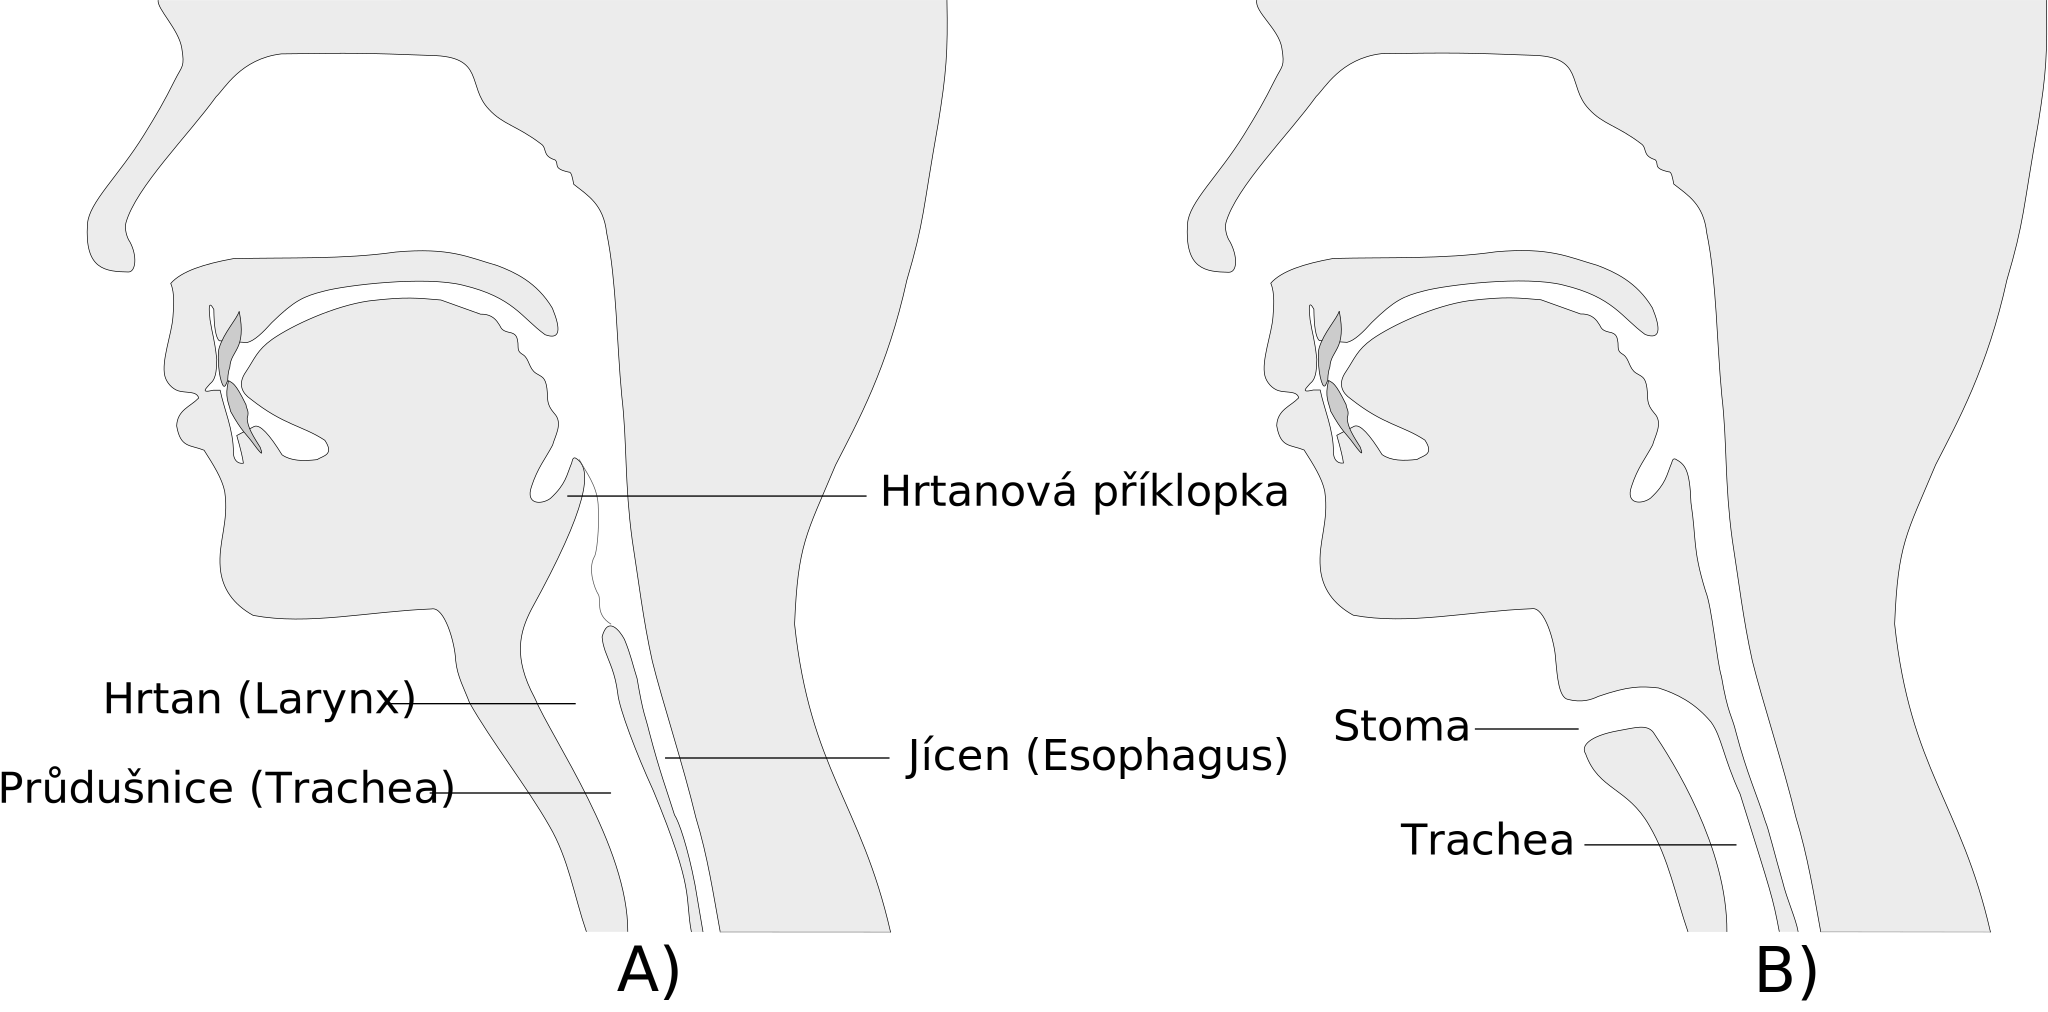
\includegraphics[width=0.9\linewidth]{ch3-cause/figures/dychaci-cesty-tl}
    \caption[Schéma dýchacích cest zdravého člověka (A) pacienta po totální laryngektomii (B)]{(A) Schéma dýchacích cest zdravého člověka (B) Schéma dýchacích cest po totální laryngektomii}
    \label{fig:cause:desease:laryngectomy}
  \end{center}
\end{figure}

Odstraněním spojení průdušnice a jícnu je zahrazena cesta vzduchu do plic.
Z~tohoto důvodu je nezbytné společně s TL vykonat také \textbf{tracheostomii}.
Cílem tohoto zákroku není léčba nádorovitého onemocnění, nýbrž vytvoření
vstupu pro vzduch směřující do plic a z~nich. Samotný zákrok se využívá i v
situacích, kdy dojde k uzávěře hrtanu a postižená osoba se dusí. K tomuto může
dojít například při alergické reakci na včelí bodnutí, otoku hrtanu, úrazu
apod. Při tracheostomii se provádí řez skrz kůži a průdušnici. Do vzniklého
otvoru se zavádí kanyla, která slouží k dýchání. Místo výkonu zákroku a
princip kanyly je znázorněn na obr. \ref{fig:cause:desease:tracheostomy}. Pro
lepší názornost je znázorněna tracheostomie se zavedenou kanylou u zdravého
člověka. Výsledek operace může být dočasný (například v případě alergické
reakce) nebo trvalý.

\begin{figure}[htb]
  \begin{center}
    \def\svgwidth{0.9\linewidth}
    % %LaTeX with PSTricks extensions
%%Creator: 0.48.3.1
%%Please note this file requires PSTricks extensions
\psset{xunit=.5pt,yunit=.5pt,runit=.5pt}
\begin{pspicture}(2907.24389648,1381.22814941)
{
\newrgbcolor{curcolor}{0.9254902 0.9254902 0.9254902}
\pscustom[linestyle=none,fillstyle=solid,fillcolor=curcolor]
{
\newpath
\moveto(70.56024,976.91215941)
\curveto(75.70194,998.05546941)(75.05233,1002.21845941)(63.72468,1022.97718941)
\curveto(59.11246,1029.25078941)(55.53152,1042.76249941)(57.82397,1051.05492941)
\curveto(72.33535,1103.54679941)(151.12483,1181.98458841)(191.6593,1238.29379441)
\curveto(203.82655,1249.22791741)(227.588336,1294.48932741)(288.348581,1301.70009441)
\curveto(395.40091,1303.19005241)(412.940729,1303.02200041)(510.35569,1299.36034741)
\curveto(591.16393,1298.04450341)(563.1446,1253.97868341)(596.12059,1219.46677821)
\curveto(617.11351,1196.64470041)(637.32731,1195.59050941)(673.24323,1168.28753341)
\curveto(683.09539,1161.70729041)(674.18628,1150.76886041)(694.17272,1144.46094641)
\curveto(700.8548,1138.26728041)(689.58524,1131.75588441)(714.56462,1126.38918541)
\curveto(718.47149,1127.09967441)(720.01648,1117.64831941)(721.82813,1108.38187941)
\curveto(742.89519,1091.67695941)(766.01459,1078.47903941)(770.6489,1036.21205941)
\curveto(785.52916,964.13363941)(785.41095,874.88456941)(793.05455,794.70262941)
\curveto(801.16608,725.36812941)(797.04543,665.20049941)(808.62059,580.55167941)
\curveto(817.99398,520.80324941)(824.99343,461.05482941)(838.33757,401.30639941)
\curveto(852.58351,343.43859941)(884.634,245.85682941)(902.96021,169.23090941)
\curveto(920.58527,111.57990941)(928.99355,58.22450941)(939.28097,2.24980941)
\lineto(1191.38979,0.50000941)
\curveto(1147.46289,192.92300941)(1072.39851,239.15118941)(1049.32187,456.03356941)
\curveto(1054.33227,575.87003941)(1066.33852,587.71091941)(1110.16719,692.25659941)
\curveto(1142.86475,756.08452941)(1187.16897,836.01858941)(1215.75173,966.06054941)
\curveto(1241.69732,1053.47858941)(1239.12891,1068.56755941)(1262.28051,1198.70444641)
\curveto(1274.15414,1272.24631941)(1276.84845,1302.56969941)(1275.20381,1380.20462941)
\curveto(1243.6598,1381.01350941)(132.01823,1379.13434941)(108.97269,1379.62040941)
\curveto(89.62734,1380.02842941)(136.091,1338.49754941)(140.67855,1310.22027841)
\curveto(145.31215,1281.65916741)(141.36641,1284.78090841)(130.36263,1262.73876141)
\curveto(114.38301,1230.72928461)(103.72405,1212.44353221)(84.57988,1181.51309641)
\curveto(46.3326,1119.71856941)(3.13314,1081.66825941)(0.88674,1049.70937941)
\curveto(-3.93696,981.08423941)(37.32565,977.54602941)(70.95213,976.84547941)
}
}
{
\newrgbcolor{curcolor}{0 0 0}
\pscustom[linewidth=1,linecolor=curcolor]
{
\newpath
\moveto(70.56024,976.91215941)
\curveto(75.70194,998.05546941)(75.05233,1002.21845941)(63.72468,1022.97718941)
\curveto(59.11246,1029.25078941)(55.53152,1042.76249941)(57.82397,1051.05492941)
\curveto(72.33535,1103.54679941)(151.12483,1181.98458841)(191.6593,1238.29379441)
\curveto(203.82655,1249.22791741)(227.588336,1294.48932741)(288.348581,1301.70009441)
\curveto(395.40091,1303.19005241)(412.940729,1303.02200041)(510.35569,1299.36034741)
\curveto(591.16393,1298.04450341)(563.1446,1253.97868341)(596.12059,1219.46677821)
\curveto(617.11351,1196.64470041)(637.32731,1195.59050941)(673.24323,1168.28753341)
\curveto(683.09539,1161.70729041)(674.18628,1150.76886041)(694.17272,1144.46094641)
\curveto(700.8548,1138.26728041)(689.58524,1131.75588441)(714.56462,1126.38918541)
\curveto(718.47149,1127.09967441)(720.01648,1117.64831941)(721.82813,1108.38187941)
\curveto(742.89519,1091.67695941)(766.01459,1078.47903941)(770.6489,1036.21205941)
\curveto(785.52916,964.13363941)(785.41095,874.88456941)(793.05455,794.70262941)
\curveto(801.16608,725.36812941)(797.04543,665.20049941)(808.62059,580.55167941)
\curveto(817.99398,520.80324941)(824.99343,461.05482941)(838.33757,401.30639941)
\curveto(852.58351,343.43859941)(884.634,245.85682941)(902.96021,169.23090941)
\curveto(920.58527,111.57990941)(928.99355,58.22450941)(939.28097,2.24980941)
\lineto(1191.38979,0.50000941)
\curveto(1147.46289,192.92300941)(1072.39851,239.15118941)(1049.32187,456.03356941)
\curveto(1054.33227,575.87003941)(1066.33852,587.71091941)(1110.16719,692.25659941)
\curveto(1142.86475,756.08452941)(1187.16897,836.01858941)(1215.75173,966.06054941)
\curveto(1241.69732,1053.47858941)(1239.12891,1068.56755941)(1262.28051,1198.70444641)
\curveto(1274.15414,1272.24631941)(1276.84845,1302.56969941)(1275.20381,1380.20462941)
\curveto(1243.6598,1381.01350941)(132.01823,1379.13434941)(108.97269,1379.62040941)
\curveto(89.62734,1380.02842941)(136.091,1338.49754941)(140.67855,1310.22027841)
\curveto(145.31215,1281.65916741)(141.36641,1284.78090841)(130.36263,1262.73876141)
\curveto(114.38301,1230.72928461)(103.72405,1212.44353221)(84.57988,1181.51309641)
\curveto(46.3326,1119.71856941)(3.13314,1081.66825941)(0.88674,1049.70937941)
\curveto(-3.93696,981.08423941)(37.32565,977.54602941)(70.95213,976.84547941)
}
}
{
\newrgbcolor{curcolor}{0.9254902 0.9254902 0.9254902}
\pscustom[linestyle=none,fillstyle=solid,fillcolor=curcolor]
{
\newpath
\moveto(663.80927,347.06111941)
\curveto(631.30672,407.78342941)(641.93353,444.78459941)(659.09229,478.19318941)
\curveto(742.49859,629.54060941)(751.64804,687.40579941)(724.24075,702.51595941)
\curveto(719.95848,704.09435941)(719.37506,696.51114941)(718.82765,695.21471941)
\curveto(711.30272,677.39364941)(710.58153,663.97482941)(687.1752,642.50022941)
\curveto(674.22342,633.07831941)(649.93085,632.99143941)(659.17482,660.02528941)
\curveto(668.2034,687.86169941)(679.75486,701.25992941)(690.49227,721.54170941)
\curveto(694.32384,735.78587941)(706.54118,754.42062941)(692.9595,768.66479941)
\curveto(680.15631,783.42381941)(684.07081,790.42534941)(682.11354,805.65799941)
\curveto(679.75193,823.26346941)(674.12318,822.66506941)(666.00743,828.02760941)
\curveto(655.05672,835.06925941)(656.16371,849.42328941)(646.73777,855.61704941)
\curveto(638.64629,860.32035941)(639.52383,863.34606941)(639.1639,872.76681941)
\curveto(637.98441,879.54741941)(638.28659,886.96301941)(625.74214,888.87292941)
\curveto(612.81159,891.73856941)(614.30292,897.00785941)(610.53081,901.39990941)
\curveto(604.8368,911.05283941)(596.12842,916.18422941)(583.68728,915.71645941)
\lineto(524.93857,936.77567941)
\curveto(490.25612,939.54036941)(474.30758,942.06391941)(418.15221,935.40170941)
\curveto(366.534745,928.00029941)(304.2199481,899.10557941)(274.750996,878.48752941)
\curveto(252.003981,862.15967941)(248.537062,849.31921941)(235.769747,830.34131941)
\curveto(222.937923,811.90137941)(230.373646,798.51614941)(242.774499,789.96747941)
\curveto(292.076635,750.86082941)(319.3103455,750.81408941)(352.832959,728.70655941)
\curveto(367.325625,706.91548941)(350.454946,706.03330941)(341.200769,700.07346941)
\curveto(321.2014438,697.73427941)(302.607692,697.85483941)(289.303279,707.23173941)
\curveto(270.762837,737.31808941)(256.564999,752.92908941)(248.143209,749.28659941)
\lineto(222.194469,735.86482941)
\curveto(228.231101,714.79611941)(231.053383,702.29899941)(232.037089,694.70475941)
\curveto(221.981864,693.29911941)(217.293619,701.68940941)(217.241359,710.28672941)
\curveto(217.477079,744.22373941)(203.2615,775.02108941)(197.55611,802.97364941)
\lineto(187.29789,802.97364941)
\curveto(166.56822,797.91572941)(178.05638,806.67132941)(182.82396,812.81626941)
\curveto(193.34887,820.71151941)(191.8352,839.37924941)(192.55804,848.77977941)
\curveto(189.01508,880.83561941)(186.10484,884.60710941)(182.56189,907.38269941)
\curveto(180.76794,924.17114941)(180.01497,937.66317941)(188.19267,922.87472941)
\curveto(188.49625,897.84202941)(190.8841,881.14644941)(196.24573,876.34594941)
\lineto(237.405799,873.66159941)
\curveto(248.143914,876.10038941)(260.863359,888.38046941)(274.091949,903.18947941)
\curveto(307.5567096,935.85866941)(321.1413212,942.22030941)(351.196907,949.82680941)
\curveto(383.523382,958.67919941)(501.87189,972.81484941)(557.73854,958.66609941)
\curveto(632.46539,940.77852941)(644.32636,910.80136941)(679.42919,885.29378941)
\curveto(701.57916,877.19347941)(703.43081,892.29125941)(690.1666,924.66429941)
\curveto(667.08021,963.46625941)(633.47421,978.37656941)(608.19846,987.93189941)
\curveto(565.49811,999.98699941)(539.14436,1015.15373941)(457.78478,1007.87922941)
\curveto(379.904483,996.64752941)(297.741184,1000.16294941)(216.825769,998.03659941)
\curveto(173.57623,990.17701941)(140.18925,979.41667941)(124.29082,961.33378941)
\curveto(130.726,946.56084941)(128.46979,924.48665941)(127.58388,911.82347941)
\curveto(125.77419,885.95569941)(110.07974,846.59298941)(115.57181,824.08208941)
\curveto(117.8965,814.55367941)(126.13355,805.09264941)(135.50065,802.07764941)
\curveto(146.31169,798.59789941)(163.07609,802.37811941)(165.7171,791.42292941)
\curveto(153.73391,778.74919941)(133.98029,773.84590941)(133.09836,750.07091941)
\curveto(138.68162,717.00597941)(153.29258,722.31734941)(173.72208,714.04142941)
\curveto(187.02623,693.18217941)(200.39377,672.31353941)(204.32814,652.84226941)
\curveto(210.9065,607.17595941)(194.37244,578.73022941)(197.73702,539.26597941)
\curveto(200.49791,508.68349941)(217.093467,485.47951941)(246.536796,469.12768941)
\curveto(327.687696,453.96820941)(416.73819,474.96141941)(510.92789,478.67598941)
\curveto(530.04251,482.78327941)(545.67914,429.27048941)(546.81162,402.15754941)
\curveto(549.12588,378.19912941)(560.21646,359.01453941)(567.26823,339.79363941)
\curveto(599.04903,283.26154941)(653.26269,213.99460941)(685.53957,157.14470941)
\curveto(714.54359,107.81710941)(724.30311,55.08410941)(742.45504,2.65910941)
\curveto(791.06479,2.93720941)(798.38877,2.65910941)(798.38877,2.65910941)
\curveto(799.22188,128.23700941)(690.30166,284.55155941)(663.80927,347.06111941)
\closepath
}
}
{
\newrgbcolor{curcolor}{0 0 0}
\pscustom[linewidth=1,linecolor=curcolor]
{
\newpath
\moveto(663.80927,347.06111941)
\curveto(631.30672,407.78342941)(641.93353,444.78459941)(659.09229,478.19318941)
\curveto(742.49859,629.54060941)(751.64804,687.40579941)(724.24075,702.51595941)
\curveto(719.95848,704.09435941)(719.37506,696.51114941)(718.82765,695.21471941)
\curveto(711.30272,677.39364941)(710.58153,663.97482941)(687.1752,642.50022941)
\curveto(674.22342,633.07831941)(649.93085,632.99143941)(659.17482,660.02528941)
\curveto(668.2034,687.86169941)(679.75486,701.25992941)(690.49227,721.54170941)
\curveto(694.32384,735.78587941)(706.54118,754.42062941)(692.9595,768.66479941)
\curveto(680.15631,783.42381941)(684.07081,790.42534941)(682.11354,805.65799941)
\curveto(679.75193,823.26346941)(674.12318,822.66506941)(666.00743,828.02760941)
\curveto(655.05672,835.06925941)(656.16371,849.42328941)(646.73777,855.61704941)
\curveto(638.64629,860.32035941)(639.52383,863.34606941)(639.1639,872.76681941)
\curveto(637.98441,879.54741941)(638.28659,886.96301941)(625.74214,888.87292941)
\curveto(612.81159,891.73856941)(614.30292,897.00785941)(610.53081,901.39990941)
\curveto(604.8368,911.05283941)(596.12842,916.18422941)(583.68728,915.71645941)
\lineto(524.93857,936.77567941)
\curveto(490.25612,939.54036941)(474.30758,942.06391941)(418.15221,935.40170941)
\curveto(366.534745,928.00029941)(304.2199481,899.10557941)(274.750996,878.48752941)
\curveto(252.003981,862.15967941)(248.537062,849.31921941)(235.769747,830.34131941)
\curveto(222.937923,811.90137941)(230.373646,798.51614941)(242.774499,789.96747941)
\curveto(292.076635,750.86082941)(319.3103455,750.81408941)(352.832959,728.70655941)
\curveto(367.325625,706.91548941)(350.454946,706.03330941)(341.200769,700.07346941)
\curveto(321.2014438,697.73427941)(302.607692,697.85483941)(289.303279,707.23173941)
\curveto(270.762837,737.31808941)(256.564999,752.92908941)(248.143209,749.28659941)
\lineto(222.194469,735.86482941)
\curveto(228.231101,714.79611941)(231.053383,702.29899941)(232.037089,694.70475941)
\curveto(221.981864,693.29911941)(217.293619,701.68940941)(217.241359,710.28672941)
\curveto(217.477079,744.22373941)(203.2615,775.02108941)(197.55611,802.97364941)
\lineto(187.29789,802.97364941)
\curveto(166.56822,797.91572941)(178.05638,806.67132941)(182.82396,812.81626941)
\curveto(193.34887,820.71151941)(191.8352,839.37924941)(192.55804,848.77977941)
\curveto(189.01508,880.83561941)(186.10484,884.60710941)(182.56189,907.38269941)
\curveto(180.76794,924.17114941)(180.01497,937.66317941)(188.19267,922.87472941)
\curveto(188.49625,897.84202941)(190.8841,881.14644941)(196.24573,876.34594941)
\lineto(237.405799,873.66159941)
\curveto(248.143914,876.10038941)(260.863359,888.38046941)(274.091949,903.18947941)
\curveto(307.5567096,935.85866941)(321.1413212,942.22030941)(351.196907,949.82680941)
\curveto(383.523382,958.67919941)(501.87189,972.81484941)(557.73854,958.66609941)
\curveto(632.46539,940.77852941)(644.32636,910.80136941)(679.42919,885.29378941)
\curveto(701.57916,877.19347941)(703.43081,892.29125941)(690.1666,924.66429941)
\curveto(667.08021,963.46625941)(633.47421,978.37656941)(608.19846,987.93189941)
\curveto(565.49811,999.98699941)(539.14436,1015.15373941)(457.78478,1007.87922941)
\curveto(379.904483,996.64752941)(297.741184,1000.16294941)(216.825769,998.03659941)
\curveto(173.57623,990.17701941)(140.18925,979.41667941)(124.29082,961.33378941)
\curveto(130.726,946.56084941)(128.46979,924.48665941)(127.58388,911.82347941)
\curveto(125.77419,885.95569941)(110.07974,846.59298941)(115.57181,824.08208941)
\curveto(117.8965,814.55367941)(126.13355,805.09264941)(135.50065,802.07764941)
\curveto(146.31169,798.59789941)(163.07609,802.37811941)(165.7171,791.42292941)
\curveto(153.73391,778.74919941)(133.98029,773.84590941)(133.09836,750.07091941)
\curveto(138.68162,717.00597941)(153.29258,722.31734941)(173.72208,714.04142941)
\curveto(187.02623,693.18217941)(200.39377,672.31353941)(204.32814,652.84226941)
\curveto(210.9065,607.17595941)(194.37244,578.73022941)(197.73702,539.26597941)
\curveto(200.49791,508.68349941)(217.093467,485.47951941)(246.536796,469.12768941)
\curveto(327.687696,453.96820941)(416.73819,474.96141941)(510.92789,478.67598941)
\curveto(530.04251,482.78327941)(545.67914,429.27048941)(546.81162,402.15754941)
\curveto(549.12588,378.19912941)(560.21646,359.01453941)(567.26823,339.79363941)
\curveto(599.04903,283.26154941)(653.26269,213.99460941)(685.53957,157.14470941)
\curveto(714.54359,107.81710941)(724.30311,55.08410941)(742.45504,2.65910941)
\curveto(791.06479,2.93720941)(798.38877,2.65910941)(798.38877,2.65910941)
\curveto(799.22188,128.23700941)(690.30166,284.55155941)(663.80927,347.06111941)
\closepath
}
}
{
\newrgbcolor{curcolor}{0.9254902 0.9254902 0.9254902}
\pscustom[linestyle=none,fillstyle=solid,fillcolor=curcolor]
{
\newpath
\moveto(895.41899,4.16750941)
\curveto(885.42628,56.53280941)(902.19573,58.71910941)(839.94237,209.07310941)
\curveto(814.28299,265.00824941)(789.33265,331.01818941)(787.1501,353.13337941)
\curveto(783.27094,384.03743941)(774.61723,398.97336941)(768.35964,416.66306941)
\curveto(765.06171,427.11926941)(764.824,429.14654941)(763.88572,437.24309941)
\curveto(772.18552,469.13804941)(790.10614,446.64287941)(796.99273,433.66395941)
\curveto(806.54018,410.67444941)(809.23317,396.02182941)(815.7832,375.50298941)
\curveto(825.27074,319.54128941)(827.96413,320.89590941)(833.67888,296.76197941)
\curveto(850.02247,234.61056941)(859.17548,212.00730941)(871.25982,173.28180941)
\curveto(877.50757,164.14560941)(890.91697,125.77240941)(901.68248,69.48680941)
\curveto(911.70975,10.97790941)(908.84075,23.55460941)(912.41989,3.27280941)
\closepath
}
}
{
\newrgbcolor{curcolor}{0 0 0}
\pscustom[linewidth=1,linecolor=curcolor]
{
\newpath
\moveto(895.41899,4.16750941)
\curveto(885.42628,56.53280941)(902.19573,58.71910941)(839.94237,209.07310941)
\curveto(814.28299,265.00824941)(789.33265,331.01818941)(787.1501,353.13337941)
\curveto(783.27094,384.03743941)(774.61723,398.97336941)(768.35964,416.66306941)
\curveto(765.06171,427.11926941)(764.824,429.14654941)(763.88572,437.24309941)
\curveto(772.18552,469.13804941)(790.10614,446.64287941)(796.99273,433.66395941)
\curveto(806.54018,410.67444941)(809.23317,396.02182941)(815.7832,375.50298941)
\curveto(825.27074,319.54128941)(827.96413,320.89590941)(833.67888,296.76197941)
\curveto(850.02247,234.61056941)(859.17548,212.00730941)(871.25982,173.28180941)
\curveto(877.50757,164.14560941)(890.91697,125.77240941)(901.68248,69.48680941)
\curveto(911.70975,10.97790941)(908.84075,23.55460941)(912.41989,3.27280941)
\closepath
}
}
{
\newrgbcolor{curcolor}{0.3019608 0.3019608 0.3019608}
\pscustom[linewidth=1,linecolor=curcolor]
{
\newpath
\moveto(777.30748,456.03356941)
\curveto(752.3253,471.35452941)(763.78475,491.53873941)(758.09534,500.48890941)
\curveto(752.61989,509.10247941)(742.51461,537.74873941)(752.25352,555.80199941)
\curveto(755.72774,560.13621941)(760.22549,596.01455941)(758.06962,633.64822941)
\curveto(756.02394,662.52158941)(739.67178,681.85842941)(729.88392,700.30964941)
}
}
{
\newrgbcolor{curcolor}{0.9254902 0.9254902 0.9254902}
\pscustom[linestyle=none,fillstyle=solid,fillcolor=curcolor]
{
\newpath
\moveto(1701.66159587,977.23068781)
\curveto(1706.80329587,998.37399781)(1706.15369587,1002.53698781)(1694.82599587,1023.29571781)
\curveto(1690.21379587,1029.56931781)(1686.63289587,1043.08102781)(1688.92529587,1051.37344781)
\curveto(1703.43669587,1103.86531781)(1782.22619587,1182.30311781)(1822.76069587,1238.61232781)
\curveto(1834.92789587,1249.54644781)(1858.68969587,1294.80786081)(1919.44989587,1302.01863081)
\curveto(2026.50229587,1303.50859081)(2044.04209587,1303.34053081)(2141.45699587,1299.67888081)
\curveto(2222.26529587,1298.36304081)(2194.24599587,1254.29721781)(2227.22189587,1219.78530781)
\curveto(2248.21489587,1196.96322781)(2268.42869587,1195.90903781)(2304.34459587,1168.60606781)
\curveto(2314.19669587,1162.02581781)(2305.28759587,1151.08738781)(2325.27409587,1144.77947781)
\curveto(2331.95619587,1138.58580781)(2320.68659587,1132.07441781)(2345.66599587,1126.70771781)
\curveto(2349.57279587,1127.41820781)(2351.11779587,1117.96683781)(2352.92949587,1108.70039781)
\curveto(2373.99649587,1091.99547781)(2397.11589587,1078.79755781)(2401.75029587,1036.53058781)
\curveto(2416.63049587,964.45216781)(2416.51229587,875.20310781)(2424.15589587,795.02115781)
\curveto(2432.26739587,725.68664781)(2428.14679587,665.51901781)(2439.72189587,580.87019781)
\curveto(2449.09529587,521.12176781)(2456.09479587,461.37334781)(2469.43889587,401.62491781)
\curveto(2483.68489587,343.75712781)(2515.73539587,246.17532781)(2534.06159587,169.54942781)
\curveto(2551.68659587,111.89842781)(2560.09489587,58.54302781)(2570.38229587,2.56832781)
\lineto(2822.49109587,0.81852781)
\curveto(2778.56419587,193.24152781)(2703.49979587,239.46972781)(2680.42319587,456.35208781)
\curveto(2685.43359587,576.18855781)(2697.43979587,588.02943781)(2741.26849587,692.57511781)
\curveto(2773.96599587,756.40305781)(2818.27029587,836.33711781)(2846.85299587,966.37907781)
\curveto(2872.79859587,1053.79710781)(2870.23019587,1068.88607781)(2893.38179587,1199.02297781)
\curveto(2905.25539587,1272.56484781)(2907.94969587,1302.88823081)(2906.30509587,1380.5231509)
\curveto(2874.76109587,1381.3320309)(1763.11959587,1379.45287091)(1740.07399587,1379.9389309)
\curveto(1720.72869587,1380.3469509)(1767.19239587,1338.81607081)(1771.77989587,1310.53881081)
\curveto(1776.41349587,1281.97770081)(1772.46779587,1285.09944081)(1761.46399587,1263.05728781)
\curveto(1745.48439587,1231.04781781)(1734.82539587,1212.76205781)(1715.68119587,1181.83162781)
\curveto(1677.43399587,1120.03708781)(1634.23449587,1081.98677781)(1631.98809587,1050.02789781)
\curveto(1627.16439587,981.40276781)(1668.42699587,977.86455781)(1702.05349587,977.16400781)
}
}
{
\newrgbcolor{curcolor}{0 0 0}
\pscustom[linewidth=1,linecolor=curcolor]
{
\newpath
\moveto(1701.66159587,977.23068781)
\curveto(1706.80329587,998.37399781)(1706.15369587,1002.53698781)(1694.82599587,1023.29571781)
\curveto(1690.21379587,1029.56931781)(1686.63289587,1043.08102781)(1688.92529587,1051.37344781)
\curveto(1703.43669587,1103.86531781)(1782.22619587,1182.30311781)(1822.76069587,1238.61232781)
\curveto(1834.92789587,1249.54644781)(1858.68969587,1294.80786081)(1919.44989587,1302.01863081)
\curveto(2026.50229587,1303.50859081)(2044.04209587,1303.34053081)(2141.45699587,1299.67888081)
\curveto(2222.26529587,1298.36304081)(2194.24599587,1254.29721781)(2227.22189587,1219.78530781)
\curveto(2248.21489587,1196.96322781)(2268.42869587,1195.90903781)(2304.34459587,1168.60606781)
\curveto(2314.19669587,1162.02581781)(2305.28759587,1151.08738781)(2325.27409587,1144.77947781)
\curveto(2331.95619587,1138.58580781)(2320.68659587,1132.07441781)(2345.66599587,1126.70771781)
\curveto(2349.57279587,1127.41820781)(2351.11779587,1117.96683781)(2352.92949587,1108.70039781)
\curveto(2373.99649587,1091.99547781)(2397.11589587,1078.79755781)(2401.75029587,1036.53058781)
\curveto(2416.63049587,964.45216781)(2416.51229587,875.20310781)(2424.15589587,795.02115781)
\curveto(2432.26739587,725.68664781)(2428.14679587,665.51901781)(2439.72189587,580.87019781)
\curveto(2449.09529587,521.12176781)(2456.09479587,461.37334781)(2469.43889587,401.62491781)
\curveto(2483.68489587,343.75712781)(2515.73539587,246.17532781)(2534.06159587,169.54942781)
\curveto(2551.68659587,111.89842781)(2560.09489587,58.54302781)(2570.38229587,2.56832781)
\lineto(2822.49109587,0.81852781)
\curveto(2778.56419587,193.24152781)(2703.49979587,239.46972781)(2680.42319587,456.35208781)
\curveto(2685.43359587,576.18855781)(2697.43979587,588.02943781)(2741.26849587,692.57511781)
\curveto(2773.96599587,756.40305781)(2818.27029587,836.33711781)(2846.85299587,966.37907781)
\curveto(2872.79859587,1053.79710781)(2870.23019587,1068.88607781)(2893.38179587,1199.02297781)
\curveto(2905.25539587,1272.56484781)(2907.94969587,1302.88823081)(2906.30509587,1380.5231509)
\curveto(2874.76109587,1381.3320309)(1763.11959587,1379.45287091)(1740.07399587,1379.9389309)
\curveto(1720.72869587,1380.3469509)(1767.19239587,1338.81607081)(1771.77989587,1310.53881081)
\curveto(1776.41349587,1281.97770081)(1772.46779587,1285.09944081)(1761.46399587,1263.05728781)
\curveto(1745.48439587,1231.04781781)(1734.82539587,1212.76205781)(1715.68119587,1181.83162781)
\curveto(1677.43399587,1120.03708781)(1634.23449587,1081.98677781)(1631.98809587,1050.02789781)
\curveto(1627.16439587,981.40276781)(1668.42699587,977.86455781)(1702.05349587,977.16400781)
}
}
{
\newrgbcolor{curcolor}{0.9254902 0.9254902 0.9254902}
\pscustom[linestyle=none,fillstyle=solid,fillcolor=curcolor]
{
\newpath
\moveto(2222.18449587,263.90192781)
\curveto(2241.31109587,209.90072781)(2284.36399587,214.31312781)(2316.64089587,157.46322781)
\curveto(2345.64489587,108.13562781)(2355.40449587,55.40262781)(2373.55639587,2.97762781)
\curveto(2422.16609587,3.25572781)(2429.49009587,2.97762781)(2429.49009587,2.97762781)
\curveto(2430.32319587,128.55552781)(2351.03939587,253.41772781)(2322.64889587,295.68062781)
\curveto(2312.63549587,308.42372781)(2295.39239587,302.39362781)(2270.51859587,298.13982781)
\curveto(2228.12249587,290.36432781)(2214.62639587,275.73032781)(2222.18449587,263.90192781)
\closepath
\moveto(2241.02189587,349.02342781)
\curveto(2285.97709587,364.43132781)(2303.47489587,364.38192781)(2330.30379587,361.55452781)
\curveto(2357.48059587,352.76802781)(2383.60959587,340.11422781)(2408.12809587,311.06042781)
\curveto(2424.23029587,288.94522781)(2445.38429587,265.32672781)(2471.04369587,209.39162781)
\curveto(2533.29709587,59.03762781)(2516.52759587,56.85132781)(2526.52029587,4.48602781)
\lineto(2543.52119587,3.59132781)
\curveto(2539.94209587,23.87312781)(2542.81109587,11.29642781)(2532.78379587,69.80532781)
\curveto(2522.01829587,126.09092781)(2508.60889587,164.46412781)(2502.36119587,173.60032781)
\curveto(2490.27679587,212.32582781)(2481.12379587,234.92902781)(2464.78019587,297.08052781)
\curveto(2459.06549587,321.21442781)(2456.37209587,319.85982781)(2446.88459587,375.82152781)
\curveto(2440.33449587,396.34034781)(2416.76219587,481.22354781)(2407.21469587,504.21305781)
\curveto(2387.67399587,567.80861781)(2386.83649587,580.18045781)(2378.38959587,636.46615781)
\curveto(2376.77379587,686.52617781)(2369.04569587,693.38127781)(2355.34209587,700.93635781)
\curveto(2351.05979587,702.51475781)(2350.47639587,696.82966781)(2349.92899587,695.53323781)
\curveto(2342.40409587,677.71216781)(2341.68289587,664.29334781)(2318.27659587,642.81874781)
\curveto(2305.32479587,633.39683781)(2281.03219587,633.30995781)(2290.27619587,660.34380781)
\curveto(2299.30479587,688.18021781)(2310.85619587,701.57844781)(2321.59359587,721.86022781)
\curveto(2325.42519587,736.10439781)(2337.64249587,754.73915781)(2324.06089587,768.98332781)
\curveto(2311.25769587,783.74234781)(2315.17219587,790.74387781)(2313.21489587,805.97652781)
\curveto(2310.85329587,823.58199781)(2305.22449587,822.98359781)(2297.10879587,828.34613781)
\curveto(2286.15809587,835.38778781)(2287.26509587,849.74182781)(2277.83909587,855.93558781)
\curveto(2269.74759587,860.63889781)(2270.62519587,863.66460781)(2270.26529587,873.08535781)
\curveto(2269.08579587,879.86595781)(2269.38789587,887.28155781)(2256.84349587,889.19146781)
\curveto(2243.91289587,892.05710781)(2245.40429587,897.32639781)(2241.63219587,901.71844781)
\curveto(2235.93819587,911.37137781)(2227.22979587,916.50276781)(2214.78859587,916.03499781)
\lineto(2156.03989587,937.09421781)
\curveto(2121.35749587,939.85890781)(2105.40889587,942.38245781)(2049.25359587,935.72024781)
\curveto(1997.63609587,928.31883781)(1935.32129587,899.42411781)(1905.85229587,878.80606781)
\curveto(1883.10529587,862.47821781)(1879.63839587,849.63775781)(1866.87109587,830.65984781)
\curveto(1854.03929587,812.21990781)(1861.47499587,798.83467781)(1873.87579587,790.28600781)
\curveto(1923.17799587,751.17934781)(1950.41169587,751.13260781)(1983.93429587,729.02507781)
\curveto(1998.42699587,707.23400781)(1981.55629587,706.35182781)(1972.30209587,700.39198781)
\curveto(1952.30279587,698.05279781)(1933.70899587,698.17335781)(1920.40459587,707.55025781)
\curveto(1901.86419587,737.63660781)(1887.66629587,753.24760781)(1879.24459587,749.60511781)
\lineto(1853.29579587,736.18334781)
\curveto(1859.33249587,715.11463781)(1862.15469587,702.61751781)(1863.13839587,695.02327781)
\curveto(1853.08319587,693.61763781)(1848.39499587,702.00792781)(1848.34269587,710.60524781)
\curveto(1848.57839587,744.54225781)(1834.36289587,775.33961781)(1828.65749587,803.29217781)
\lineto(1818.39919587,803.29217781)
\curveto(1797.66959587,798.23425781)(1809.15769587,806.98985781)(1813.92529587,813.13479781)
\curveto(1824.45019587,821.03004781)(1822.93659587,839.69777781)(1823.65939587,849.09831781)
\curveto(1820.11639587,881.15415781)(1817.20619587,884.92564781)(1813.66319587,907.70123781)
\curveto(1811.86929587,924.48968781)(1811.11629587,937.98171781)(1819.29399587,923.19326781)
\curveto(1819.59759587,898.16056781)(1821.98549587,881.46498781)(1827.34709587,876.66448781)
\lineto(1868.50709587,873.98013781)
\curveto(1879.24529587,876.41892781)(1891.96469587,888.69900781)(1905.19329587,903.50801781)
\curveto(1938.65809587,936.17720781)(1952.24269587,942.53884781)(1982.29829587,950.14534781)
\curveto(2014.62469587,958.99772781)(2132.97319587,973.13337781)(2188.83989587,958.98462781)
\curveto(2263.56669587,941.09706781)(2275.42769587,911.11990781)(2310.53049587,885.61232781)
\curveto(2332.68049587,877.51201781)(2334.53219587,892.60979781)(2321.26799587,924.98283781)
\curveto(2298.18159587,963.78478781)(2264.57559587,978.69509781)(2239.29979587,988.25042781)
\curveto(2196.59949587,1000.30552781)(2170.24569587,1015.47226781)(2088.88609587,1008.19775781)
\curveto(2011.00579587,996.96605781)(1928.84249587,1000.48147781)(1847.92709587,998.35512781)
\curveto(1804.67759587,990.49554781)(1771.29059587,979.73520781)(1755.39219587,961.65231781)
\curveto(1761.82739587,946.87938781)(1759.57109587,924.80519781)(1758.68519587,912.14201781)
\curveto(1756.87549587,886.27423781)(1741.18109587,846.91151781)(1746.67319587,824.40061781)
\curveto(1748.99789587,814.87220781)(1757.23489587,805.41117781)(1766.60199587,802.39617781)
\curveto(1777.41299587,798.91642781)(1794.17739587,802.69664781)(1796.81849587,791.74145781)
\curveto(1784.83529587,779.06772781)(1765.08159587,774.16443781)(1764.19969587,750.38943781)
\curveto(1769.78299587,717.32449781)(1784.39389587,722.63586781)(1804.82339587,714.35994781)
\curveto(1818.12759587,693.50069781)(1831.49509587,672.63205781)(1835.42949587,653.16078781)
\curveto(1842.00789587,607.49447781)(1825.47379587,579.04874781)(1828.83839587,539.58449781)
\curveto(1831.59929587,509.00201781)(1848.19479587,485.79803781)(1877.63809587,469.44620781)
\curveto(1958.78899587,454.28672781)(2047.83949587,475.27993781)(2142.02919587,478.99450781)
\curveto(2161.14389587,483.10179781)(2176.78049587,429.58900781)(2177.91299587,402.47606781)
\curveto(2180.22719587,378.51762781)(2182.50489587,347.35652781)(2195.88369587,344.58602781)
\curveto(2216.40419587,339.36112781)(2230.61569587,343.95892781)(2241.02189587,349.02342781)
\closepath
}
}
{
\newrgbcolor{curcolor}{0 0 0}
\pscustom[linewidth=1,linecolor=curcolor]
{
\newpath
\moveto(2222.18449587,263.90192781)
\curveto(2241.31109587,209.90072781)(2284.36399587,214.31312781)(2316.64089587,157.46322781)
\curveto(2345.64489587,108.13562781)(2355.40449587,55.40262781)(2373.55639587,2.97762781)
\curveto(2422.16609587,3.25572781)(2429.49009587,2.97762781)(2429.49009587,2.97762781)
\curveto(2430.32319587,128.55552781)(2351.03939587,253.41772781)(2322.64889587,295.68062781)
\curveto(2312.63549587,308.42372781)(2295.39239587,302.39362781)(2270.51859587,298.13982781)
\curveto(2228.12249587,290.36432781)(2214.62639587,275.73032781)(2222.18449587,263.90192781)
\closepath
\moveto(2241.02189587,349.02342781)
\curveto(2285.97709587,364.43132781)(2303.47489587,364.38192781)(2330.30379587,361.55452781)
\curveto(2357.48059587,352.76802781)(2383.60959587,340.11422781)(2408.12809587,311.06042781)
\curveto(2424.23029587,288.94522781)(2445.38429587,265.32672781)(2471.04369587,209.39162781)
\curveto(2533.29709587,59.03762781)(2516.52759587,56.85132781)(2526.52029587,4.48602781)
\lineto(2543.52119587,3.59132781)
\curveto(2539.94209587,23.87312781)(2542.81109587,11.29642781)(2532.78379587,69.80532781)
\curveto(2522.01829587,126.09092781)(2508.60889587,164.46412781)(2502.36119587,173.60032781)
\curveto(2490.27679587,212.32582781)(2481.12379587,234.92902781)(2464.78019587,297.08052781)
\curveto(2459.06549587,321.21442781)(2456.37209587,319.85982781)(2446.88459587,375.82152781)
\curveto(2440.33449587,396.34034781)(2416.76219587,481.22354781)(2407.21469587,504.21305781)
\curveto(2387.67399587,567.80861781)(2386.83649587,580.18045781)(2378.38959587,636.46615781)
\curveto(2376.77379587,686.52617781)(2369.04569587,693.38127781)(2355.34209587,700.93635781)
\curveto(2351.05979587,702.51475781)(2350.47639587,696.82966781)(2349.92899587,695.53323781)
\curveto(2342.40409587,677.71216781)(2341.68289587,664.29334781)(2318.27659587,642.81874781)
\curveto(2305.32479587,633.39683781)(2281.03219587,633.30995781)(2290.27619587,660.34380781)
\curveto(2299.30479587,688.18021781)(2310.85619587,701.57844781)(2321.59359587,721.86022781)
\curveto(2325.42519587,736.10439781)(2337.64249587,754.73915781)(2324.06089587,768.98332781)
\curveto(2311.25769587,783.74234781)(2315.17219587,790.74387781)(2313.21489587,805.97652781)
\curveto(2310.85329587,823.58199781)(2305.22449587,822.98359781)(2297.10879587,828.34613781)
\curveto(2286.15809587,835.38778781)(2287.26509587,849.74182781)(2277.83909587,855.93558781)
\curveto(2269.74759587,860.63889781)(2270.62519587,863.66460781)(2270.26529587,873.08535781)
\curveto(2269.08579587,879.86595781)(2269.38789587,887.28155781)(2256.84349587,889.19146781)
\curveto(2243.91289587,892.05710781)(2245.40429587,897.32639781)(2241.63219587,901.71844781)
\curveto(2235.93819587,911.37137781)(2227.22979587,916.50276781)(2214.78859587,916.03499781)
\lineto(2156.03989587,937.09421781)
\curveto(2121.35749587,939.85890781)(2105.40889587,942.38245781)(2049.25359587,935.72024781)
\curveto(1997.63609587,928.31883781)(1935.32129587,899.42411781)(1905.85229587,878.80606781)
\curveto(1883.10529587,862.47821781)(1879.63839587,849.63775781)(1866.87109587,830.65984781)
\curveto(1854.03929587,812.21990781)(1861.47499587,798.83467781)(1873.87579587,790.28600781)
\curveto(1923.17799587,751.17934781)(1950.41169587,751.13260781)(1983.93429587,729.02507781)
\curveto(1998.42699587,707.23400781)(1981.55629587,706.35182781)(1972.30209587,700.39198781)
\curveto(1952.30279587,698.05279781)(1933.70899587,698.17335781)(1920.40459587,707.55025781)
\curveto(1901.86419587,737.63660781)(1887.66629587,753.24760781)(1879.24459587,749.60511781)
\lineto(1853.29579587,736.18334781)
\curveto(1859.33249587,715.11463781)(1862.15469587,702.61751781)(1863.13839587,695.02327781)
\curveto(1853.08319587,693.61763781)(1848.39499587,702.00792781)(1848.34269587,710.60524781)
\curveto(1848.57839587,744.54225781)(1834.36289587,775.33961781)(1828.65749587,803.29217781)
\lineto(1818.39919587,803.29217781)
\curveto(1797.66959587,798.23425781)(1809.15769587,806.98985781)(1813.92529587,813.13479781)
\curveto(1824.45019587,821.03004781)(1822.93659587,839.69777781)(1823.65939587,849.09831781)
\curveto(1820.11639587,881.15415781)(1817.20619587,884.92564781)(1813.66319587,907.70123781)
\curveto(1811.86929587,924.48968781)(1811.11629587,937.98171781)(1819.29399587,923.19326781)
\curveto(1819.59759587,898.16056781)(1821.98549587,881.46498781)(1827.34709587,876.66448781)
\lineto(1868.50709587,873.98013781)
\curveto(1879.24529587,876.41892781)(1891.96469587,888.69900781)(1905.19329587,903.50801781)
\curveto(1938.65809587,936.17720781)(1952.24269587,942.53884781)(1982.29829587,950.14534781)
\curveto(2014.62469587,958.99772781)(2132.97319587,973.13337781)(2188.83989587,958.98462781)
\curveto(2263.56669587,941.09706781)(2275.42769587,911.11990781)(2310.53049587,885.61232781)
\curveto(2332.68049587,877.51201781)(2334.53219587,892.60979781)(2321.26799587,924.98283781)
\curveto(2298.18159587,963.78478781)(2264.57559587,978.69509781)(2239.29979587,988.25042781)
\curveto(2196.59949587,1000.30552781)(2170.24569587,1015.47226781)(2088.88609587,1008.19775781)
\curveto(2011.00579587,996.96605781)(1928.84249587,1000.48147781)(1847.92709587,998.35512781)
\curveto(1804.67759587,990.49554781)(1771.29059587,979.73520781)(1755.39219587,961.65231781)
\curveto(1761.82739587,946.87938781)(1759.57109587,924.80519781)(1758.68519587,912.14201781)
\curveto(1756.87549587,886.27423781)(1741.18109587,846.91151781)(1746.67319587,824.40061781)
\curveto(1748.99789587,814.87220781)(1757.23489587,805.41117781)(1766.60199587,802.39617781)
\curveto(1777.41299587,798.91642781)(1794.17739587,802.69664781)(1796.81849587,791.74145781)
\curveto(1784.83529587,779.06772781)(1765.08159587,774.16443781)(1764.19969587,750.38943781)
\curveto(1769.78299587,717.32449781)(1784.39389587,722.63586781)(1804.82339587,714.35994781)
\curveto(1818.12759587,693.50069781)(1831.49509587,672.63205781)(1835.42949587,653.16078781)
\curveto(1842.00789587,607.49447781)(1825.47379587,579.04874781)(1828.83839587,539.58449781)
\curveto(1831.59929587,509.00201781)(1848.19479587,485.79803781)(1877.63809587,469.44620781)
\curveto(1958.78899587,454.28672781)(2047.83949587,475.27993781)(2142.02919587,478.99450781)
\curveto(2161.14389587,483.10179781)(2176.78049587,429.58900781)(2177.91299587,402.47606781)
\curveto(2180.22719587,378.51762781)(2182.50489587,347.35652781)(2195.88369587,344.58602781)
\curveto(2216.40419587,339.36112781)(2230.61569587,343.95892781)(2241.02189587,349.02342781)
\closepath
}
}
{
\newrgbcolor{curcolor}{0.80000001 0.80000001 0.80000001}
\pscustom[linestyle=none,fillstyle=solid,fillcolor=curcolor]
{
\newpath
\moveto(1856.91629587,920.33095781)
\curveto(1852.97789587,908.04444781)(1834.19749587,888.87896781)(1827.17899587,865.91806781)
\curveto(1825.13979587,861.15995781)(1825.04509587,833.60610781)(1830.34249587,816.56683781)
\curveto(1835.47639587,800.05400781)(1837.88419587,815.66513781)(1839.83319587,817.19954781)
\curveto(1840.15089587,828.36895781)(1841.50219587,833.33705781)(1842.99669587,837.44620781)
\curveto(1844.41779587,863.38058781)(1868.34079587,862.30071781)(1856.91629587,920.33095781)
\closepath
}
}
{
\newrgbcolor{curcolor}{0 0 0}
\pscustom[linewidth=1,linecolor=curcolor]
{
\newpath
\moveto(1856.91629587,920.33095781)
\curveto(1852.97789587,908.04444781)(1834.19749587,888.87896781)(1827.17899587,865.91806781)
\curveto(1825.13979587,861.15995781)(1825.04509587,833.60610781)(1830.34249587,816.56683781)
\curveto(1835.47639587,800.05400781)(1837.88419587,815.66513781)(1839.83319587,817.19954781)
\curveto(1840.15089587,828.36895781)(1841.50219587,833.33705781)(1842.99669587,837.44620781)
\curveto(1844.41779587,863.38058781)(1868.34079587,862.30071781)(1856.91629587,920.33095781)
\closepath
}
}
{
\newrgbcolor{curcolor}{0.80000001 0.80000001 0.80000001}
\pscustom[linestyle=none,fillstyle=solid,fillcolor=curcolor]
{
\newpath
\moveto(1841.06769587,817.50097781)
\curveto(1834.91779587,792.39807781)(1841.57179587,784.90070781)(1844.19949587,771.86697781)
\curveto(1861.53959587,740.38321781)(1867.17519587,739.33153781)(1878.64859587,723.10122781)
\curveto(1894.86219587,701.16965781)(1890.18049587,711.88679781)(1888.04389587,718.62730781)
\curveto(1878.82579587,733.44367781)(1868.79449587,748.36168781)(1868.80599587,762.02435781)
\curveto(1872.25039587,772.62703781)(1867.57169587,775.10654781)(1867.01649587,781.70960781)
\curveto(1850.58659587,815.68321781)(1846.85249587,813.68698781)(1841.06769587,817.50097781)
\closepath
}
}
{
\newrgbcolor{curcolor}{0 0 0}
\pscustom[linewidth=1,linecolor=curcolor]
{
\newpath
\moveto(1841.06769587,817.50097781)
\curveto(1834.91779587,792.39807781)(1841.57179587,784.90070781)(1844.19949587,771.86697781)
\curveto(1861.53959587,740.38321781)(1867.17519587,739.33153781)(1878.64859587,723.10122781)
\curveto(1894.86219587,701.16965781)(1890.18049587,711.88679781)(1888.04389587,718.62730781)
\curveto(1878.82579587,733.44367781)(1868.79449587,748.36168781)(1868.80599587,762.02435781)
\curveto(1872.25039587,772.62703781)(1867.57169587,775.10654781)(1867.01649587,781.70960781)
\curveto(1850.58659587,815.68321781)(1846.85249587,813.68698781)(1841.06769587,817.50097781)
\closepath
}
}
{
\newrgbcolor{curcolor}{0.80000001 0.80000001 0.80000001}
\pscustom[linestyle=none,fillstyle=solid,fillcolor=curcolor]
{
\newpath
\moveto(225.814918,920.01241941)
\curveto(221.876528,907.72590941)(203.09611,888.56042941)(196.07765,865.59952941)
\curveto(194.03846,860.84141941)(193.9437,833.28757941)(199.24119,816.24830941)
\curveto(204.37501,799.73547941)(206.78283,815.34660941)(208.73181,816.88101941)
\curveto(209.04957,828.05042941)(210.40088,833.01852941)(211.89535,837.12767941)
\curveto(213.31641,863.06204941)(237.239466,861.98217941)(225.814918,920.01241941)
\closepath
}
}
{
\newrgbcolor{curcolor}{0 0 0}
\pscustom[linewidth=1,linecolor=curcolor]
{
\newpath
\moveto(225.814918,920.01241941)
\curveto(221.876528,907.72590941)(203.09611,888.56042941)(196.07765,865.59952941)
\curveto(194.03846,860.84141941)(193.9437,833.28757941)(199.24119,816.24830941)
\curveto(204.37501,799.73547941)(206.78283,815.34660941)(208.73181,816.88101941)
\curveto(209.04957,828.05042941)(210.40088,833.01852941)(211.89535,837.12767941)
\curveto(213.31641,863.06204941)(237.239466,861.98217941)(225.814918,920.01241941)
\closepath
}
}
{
\newrgbcolor{curcolor}{0.80000001 0.80000001 0.80000001}
\pscustom[linestyle=none,fillstyle=solid,fillcolor=curcolor]
{
\newpath
\moveto(209.96636,817.18244941)
\curveto(203.81641,792.07954941)(210.47048,784.58217941)(213.09811,771.54844941)
\curveto(230.438288,740.06469941)(236.073825,739.01301941)(247.547296,722.78270941)
\curveto(263.760808,700.85113941)(259.079151,711.56827941)(256.94253,718.30878941)
\curveto(247.724425,733.12515941)(237.693145,748.04316941)(237.70467,761.70582941)
\curveto(241.149079,772.30850941)(236.47031,774.78801941)(235.915102,781.39107941)
\curveto(219.485298,815.36468941)(215.751198,813.36845941)(209.96636,817.18244941)
\closepath
}
}
{
\newrgbcolor{curcolor}{0 0 0}
\pscustom[linewidth=1,linecolor=curcolor]
{
\newpath
\moveto(209.96636,817.18244941)
\curveto(203.81641,792.07954941)(210.47048,784.58217941)(213.09811,771.54844941)
\curveto(230.438288,740.06469941)(236.073825,739.01301941)(247.547296,722.78270941)
\curveto(263.760808,700.85113941)(259.079151,711.56827941)(256.94253,718.30878941)
\curveto(247.724425,733.12515941)(237.693145,748.04316941)(237.70467,761.70582941)
\curveto(241.149079,772.30850941)(236.47031,774.78801941)(235.915102,781.39107941)
\curveto(219.485298,815.36468941)(215.751198,813.36845941)(209.96636,817.18244941)
\closepath
}
}
{
\newrgbcolor{curcolor}{0 0 0}
\pscustom[linestyle=none,fillstyle=solid,fillcolor=curcolor]
{
\newpath
\moveto(35.93132134,187.90693012)
\lineto(35.93132134,222.26630512)
\lineto(48.89225884,222.26630512)
\curveto(51.17348989,222.26627076)(52.91567565,222.15689587)(54.11882134,221.93818012)
\curveto(55.80629776,221.65689637)(57.22035885,221.12174066)(58.36100884,220.33271137)
\curveto(59.50160656,219.54361724)(60.4195744,218.43814959)(61.11491509,217.01630512)
\curveto(61.81019801,215.59440243)(62.15785391,214.031904)(62.15788384,212.32880512)
\curveto(62.15785391,209.40690862)(61.22816734,206.93425484)(59.36882134,204.91083637)
\curveto(57.50942106,202.88738389)(54.15004942,201.87566615)(49.29069634,201.87568012)
\lineto(40.47819634,201.87568012)
\lineto(40.47819634,187.90693012)
\closepath
\moveto(40.47819634,205.93036762)
\lineto(49.36100884,205.93036762)
\curveto(52.29848877,205.9303496)(54.38442418,206.47722405)(55.61882134,207.57099262)
\curveto(56.85317171,208.66472186)(57.4703586,210.20378282)(57.47038384,212.18818012)
\curveto(57.4703586,213.6256544)(57.10707771,214.85612192)(56.38054009,215.87958637)
\curveto(55.65395416,216.90299488)(54.69692387,217.57877545)(53.50944634,217.90693012)
\curveto(52.74380082,218.11002492)(51.32973974,218.21158732)(49.26725884,218.21161762)
\lineto(40.47819634,218.21161762)
\closepath
}
}
{
\newrgbcolor{curcolor}{0 0 0}
\pscustom[linestyle=none,fillstyle=solid,fillcolor=curcolor]
{
\newpath
\moveto(67.40788384,187.90693012)
\lineto(67.40788384,212.79755512)
\lineto(71.20475884,212.79755512)
\lineto(71.20475884,209.02411762)
\curveto(72.17350095,210.78971974)(73.06803131,211.95378107)(73.88835259,212.51630512)
\curveto(74.70865467,213.07877995)(75.61099752,213.36002967)(76.59538384,213.36005512)
\curveto(78.01724511,213.36002967)(79.46255617,212.90690512)(80.93132134,212.00068012)
\lineto(79.47819634,208.08661762)
\curveto(78.44693218,208.69597183)(77.41568321,209.00065903)(76.38444634,209.00068012)
\curveto(75.46256017,209.00065903)(74.63443599,208.72331556)(73.90007134,208.16864887)
\curveto(73.16568746,207.61394166)(72.64225049,206.84441118)(72.32975884,205.86005512)
\curveto(71.86100127,204.36003867)(71.6266265,202.71941531)(71.62663384,200.93818012)
\lineto(71.62663384,187.90693012)
\closepath
}
}
{
\newrgbcolor{curcolor}{0 0 0}
\pscustom[linestyle=none,fillstyle=solid,fillcolor=curcolor]
{
\newpath
\moveto(99.79850884,187.90693012)
\lineto(99.79850884,191.56318012)
\curveto(97.8609913,188.75067928)(95.22818143,187.34443068)(91.90007134,187.34443012)
\curveto(90.43131123,187.34443068)(89.06021885,187.6256804)(87.78679009,188.18818012)
\curveto(86.5133464,188.75067928)(85.56803484,189.45770982)(84.95085259,190.30927387)
\curveto(84.33366108,191.16083312)(83.90006776,192.20380082)(83.65007134,193.43818012)
\curveto(83.47819318,194.26629876)(83.39225577,195.57879745)(83.39225884,197.37568012)
\lineto(83.39225884,212.79755512)
\lineto(87.61100884,212.79755512)
\lineto(87.61100884,198.99286762)
\curveto(87.61100155,196.78973374)(87.69693896,195.30536022)(87.86882134,194.53974262)
\curveto(88.13443853,193.4303621)(88.69693796,192.55926922)(89.55632134,191.92646137)
\curveto(90.41568624,191.29364549)(91.47818518,190.97723955)(92.74382134,190.97724262)
\curveto(94.00943265,190.97723955)(95.19693146,191.30145798)(96.30632134,191.94989887)
\curveto(97.41567924,192.59833168)(98.20083471,193.4811433)(98.66179009,194.59833637)
\curveto(99.12270879,195.71551606)(99.35317731,197.33660819)(99.35319634,199.46161762)
\lineto(99.35319634,212.79755512)
\lineto(103.57194634,212.79755512)
\lineto(103.57194634,187.90693012)
\closepath
\moveto(89.27507134,219.26630512)
\curveto(89.27506238,220.40689762)(89.69303072,221.39127164)(90.52897759,222.21943012)
\curveto(91.36490404,223.04751998)(92.35318431,223.46158207)(93.49382134,223.46161762)
\curveto(94.65005701,223.46158207)(95.64224352,223.04361374)(96.47038384,222.20771137)
\curveto(97.29849186,221.37174041)(97.71255395,220.36002267)(97.71257134,219.17255512)
\curveto(97.71255395,217.96940006)(97.29849186,216.95377607)(96.47038384,216.12568012)
\curveto(95.64224352,215.29752773)(94.6578695,214.88346565)(93.51725884,214.88349262)
\curveto(92.34537181,214.88346565)(91.34537281,215.30143398)(90.51725884,216.13739887)
\curveto(89.68912447,216.97330731)(89.27506238,218.01627501)(89.27507134,219.26630512)
\closepath
\moveto(91.05632134,219.24286762)
\curveto(91.0563106,218.50846202)(91.30240411,217.89127514)(91.79460259,217.39130512)
\curveto(92.28677812,216.89127614)(92.86880879,216.64127639)(93.54069634,216.64130512)
\curveto(94.21255745,216.64127639)(94.79458812,216.89127614)(95.28679009,217.39130512)
\curveto(95.77896213,217.89127514)(96.02505563,218.49283704)(96.02507134,219.19599262)
\curveto(96.02505563,219.89908563)(95.78286838,220.50064753)(95.29850884,221.00068012)
\curveto(94.81411935,221.50064653)(94.22818243,221.75064628)(93.54069634,221.75068012)
\curveto(92.86880879,221.75064628)(92.28677812,221.50455277)(91.79460259,221.01239887)
\curveto(91.30240411,220.52017876)(91.0563106,219.9303356)(91.05632134,219.24286762)
\closepath
}
}
{
\newrgbcolor{curcolor}{0 0 0}
\pscustom[linestyle=none,fillstyle=solid,fillcolor=curcolor]
{
\newpath
\moveto(126.35319634,187.90693012)
\lineto(126.35319634,191.04755512)
\curveto(124.7750536,188.57880445)(122.45474342,187.34443068)(119.39225884,187.34443012)
\curveto(117.40787347,187.34443068)(115.58365654,187.89130514)(113.91960259,188.98505512)
\curveto(112.25553487,190.07880295)(110.96647366,191.60614517)(110.05241509,193.56708637)
\curveto(109.13835049,195.52801625)(108.6813197,197.78192025)(108.68132134,200.32880512)
\curveto(108.6813197,202.81316522)(109.09538178,205.06706921)(109.92350884,207.09052387)
\curveto(110.75163013,209.11394016)(111.99381638,210.66471986)(113.65007134,211.74286762)
\curveto(115.30631307,212.82096771)(117.15787372,213.36002967)(119.20475884,213.36005512)
\curveto(120.70474517,213.36002967)(122.04068134,213.04362374)(123.21257134,212.41083637)
\curveto(124.38442899,211.778)(125.33755304,210.95378207)(126.07194634,209.93818012)
\lineto(126.07194634,222.26630512)
\lineto(130.26725884,222.26630512)
\lineto(130.26725884,187.90693012)
\closepath
\moveto(113.01725884,200.32880512)
\curveto(113.01725286,197.14129589)(113.68912719,194.75848577)(115.03288384,193.18036762)
\curveto(116.3766245,191.60223893)(117.96256042,190.81317722)(119.79069634,190.81318012)
\curveto(121.63443174,190.81317722)(123.20083643,191.56708271)(124.48991509,193.07489887)
\curveto(125.77895885,194.5827047)(126.42348945,196.88348365)(126.42350884,199.97724262)
\curveto(126.42348945,203.38347715)(125.76724011,205.88347465)(124.45475884,207.47724262)
\curveto(123.14224274,209.07097146)(121.52505685,209.86784566)(119.60319634,209.86786762)
\curveto(117.72818565,209.86784566)(116.16178097,209.10222143)(114.90397759,207.57099262)
\curveto(113.64615848,206.03972449)(113.01725286,203.6256644)(113.01725884,200.32880512)
\closepath
}
}
{
\newrgbcolor{curcolor}{0 0 0}
\pscustom[linestyle=none,fillstyle=solid,fillcolor=curcolor]
{
\newpath
\moveto(153.23600884,187.90693012)
\lineto(153.23600884,191.56318012)
\curveto(151.2984913,188.75067928)(148.66568143,187.34443068)(145.33757134,187.34443012)
\curveto(143.86881123,187.34443068)(142.49771885,187.6256804)(141.22429009,188.18818012)
\curveto(139.9508464,188.75067928)(139.00553484,189.45770982)(138.38835259,190.30927387)
\curveto(137.77116108,191.16083312)(137.33756776,192.20380082)(137.08757134,193.43818012)
\curveto(136.91569318,194.26629876)(136.82975577,195.57879745)(136.82975884,197.37568012)
\lineto(136.82975884,212.79755512)
\lineto(141.04850884,212.79755512)
\lineto(141.04850884,198.99286762)
\curveto(141.04850155,196.78973374)(141.13443896,195.30536022)(141.30632134,194.53974262)
\curveto(141.57193853,193.4303621)(142.13443796,192.55926922)(142.99382134,191.92646137)
\curveto(143.85318624,191.29364549)(144.91568518,190.97723955)(146.18132134,190.97724262)
\curveto(147.44693265,190.97723955)(148.63443146,191.30145798)(149.74382134,191.94989887)
\curveto(150.85317924,192.59833168)(151.63833471,193.4811433)(152.09929009,194.59833637)
\curveto(152.56020879,195.71551606)(152.79067731,197.33660819)(152.79069634,199.46161762)
\lineto(152.79069634,212.79755512)
\lineto(157.00944634,212.79755512)
\lineto(157.00944634,187.90693012)
\closepath
}
}
{
\newrgbcolor{curcolor}{0 0 0}
\pscustom[linestyle=none,fillstyle=solid,fillcolor=curcolor]
{
\newpath
\moveto(161.95475884,195.33661762)
\lineto(166.12663384,195.99286762)
\curveto(166.36100295,194.32098621)(167.01334605,193.03973749)(168.08366509,192.14911762)
\curveto(169.15396891,191.25848927)(170.65006117,190.81317722)(172.57194634,190.81318012)
\curveto(174.50943231,190.81317722)(175.94693087,191.20770807)(176.88444634,191.99677387)
\curveto(177.82192899,192.78583149)(178.29067853,193.71161182)(178.29069634,194.77411762)
\curveto(178.29067853,195.7272348)(177.87661644,196.47723405)(177.04850884,197.02411762)
\curveto(176.47036785,197.39910813)(175.03286928,197.87567015)(172.73600884,198.45380512)
\curveto(169.64224967,199.23504379)(167.49772057,199.91082437)(166.30241509,200.48114887)
\curveto(165.10709796,201.05144823)(164.20084887,201.84050994)(163.58366509,202.84833637)
\curveto(162.9664751,203.85613292)(162.65788166,204.96941306)(162.65788384,206.18818012)
\curveto(162.65788166,207.29753573)(162.91178765,208.32487845)(163.41960259,209.27021137)
\curveto(163.92741164,210.21550156)(164.6188172,211.00065703)(165.49382134,211.62568012)
\curveto(166.15006567,212.11003092)(167.04459602,212.52018676)(168.17741509,212.85614887)
\curveto(169.31021876,213.19206109)(170.52506129,213.36002967)(171.82194634,213.36005512)
\curveto(173.77505804,213.36002967)(175.48990008,213.07877995)(176.96647759,212.51630512)
\curveto(178.44302212,211.95378107)(179.53286478,211.19206309)(180.23600884,210.23114887)
\curveto(180.93911338,209.27019001)(181.42348789,207.98503504)(181.68913384,206.37568012)
\lineto(177.56413384,205.81318012)
\curveto(177.37661694,207.09441093)(176.83364873,208.09440993)(175.93522759,208.81318012)
\curveto(175.03677553,209.5319085)(173.76724555,209.89128314)(172.12663384,209.89130512)
\curveto(170.18912413,209.89128314)(168.80631301,209.57097096)(167.97819634,208.93036762)
\curveto(167.15006467,208.28972224)(166.73600258,207.53972299)(166.73600884,206.68036762)
\curveto(166.73600258,206.1334744)(166.90787741,205.64128739)(167.25163384,205.20380512)
\curveto(167.59537672,204.75066328)(168.13443868,204.37566365)(168.86882134,204.07880512)
\curveto(169.29068753,203.92253911)(170.53287378,203.56316447)(172.59538384,203.00068012)
\curveto(175.57974374,202.20379082)(177.6617729,201.55144773)(178.84147759,201.04364887)
\curveto(180.02114554,200.53582374)(180.94692587,199.79754323)(181.61882134,198.82880512)
\curveto(182.29067453,197.86004517)(182.62661169,196.65692137)(182.62663384,195.21943012)
\curveto(182.62661169,193.81317422)(182.21645585,192.48895679)(181.39616509,191.24677387)
\curveto(180.57583249,190.00458427)(179.39223992,189.04364774)(177.84538384,188.36396137)
\curveto(176.29849302,187.68427409)(174.54849477,187.34443068)(172.59538384,187.34443012)
\curveto(169.36099995,187.34443068)(166.89615867,188.01630501)(165.20085259,189.36005512)
\curveto(163.50553706,190.70380232)(162.42350689,192.69598783)(161.95475884,195.33661762)
\closepath
\moveto(172.36100884,218.46943012)
\lineto(174.93913384,222.45380512)
\lineto(179.72038384,222.45380512)
\lineto(174.44694634,215.89130512)
\lineto(169.94694634,215.89130512)
\lineto(164.88444634,222.45380512)
\lineto(169.71257134,222.45380512)
\closepath
}
}
{
\newrgbcolor{curcolor}{0 0 0}
\pscustom[linestyle=none,fillstyle=solid,fillcolor=curcolor]
{
\newpath
\moveto(187.64225884,187.90693012)
\lineto(187.64225884,212.79755512)
\lineto(191.43913384,212.79755512)
\lineto(191.43913384,209.25849262)
\curveto(193.26725005,211.99284354)(195.90787241,213.36002967)(199.36100884,213.36005512)
\curveto(200.86099245,213.36002967)(202.23989733,213.09049869)(203.49772759,212.55146137)
\curveto(204.75551981,212.01237477)(205.69692512,211.30534422)(206.32194634,210.43036762)
\curveto(206.94692387,209.55534597)(207.38442343,208.51628451)(207.63444634,207.31318012)
\curveto(207.79067303,206.5319115)(207.86879795,205.16472536)(207.86882134,203.21161762)
\lineto(207.86882134,187.90693012)
\lineto(203.65007134,187.90693012)
\lineto(203.65007134,203.04755512)
\curveto(203.65005217,204.76628826)(203.48598983,206.05144323)(203.15788384,206.90302387)
\curveto(202.82974049,207.75456652)(202.24770982,208.43425334)(201.41179009,208.94208637)
\curveto(200.57583649,209.44987733)(199.59536872,209.70378332)(198.47038384,209.70380512)
\curveto(196.67349664,209.70378332)(195.12271694,209.1334714)(193.81804009,207.99286762)
\curveto(192.51334455,206.85222368)(191.86100145,204.68816334)(191.86100884,201.50068012)
\lineto(191.86100884,187.90693012)
\closepath
}
}
{
\newrgbcolor{curcolor}{0 0 0}
\pscustom[linestyle=none,fillstyle=solid,fillcolor=curcolor]
{
\newpath
\moveto(214.38444634,217.41474262)
\lineto(214.38444634,222.26630512)
\lineto(218.60319634,222.26630512)
\lineto(218.60319634,217.41474262)
\closepath
\moveto(214.38444634,187.90693012)
\lineto(214.38444634,212.79755512)
\lineto(218.60319634,212.79755512)
\lineto(218.60319634,187.90693012)
\closepath
}
}
{
\newrgbcolor{curcolor}{0 0 0}
\pscustom[linestyle=none,fillstyle=solid,fillcolor=curcolor]
{
\newpath
\moveto(241.29069634,197.02411762)
\lineto(245.43913384,196.48505512)
\curveto(244.98598574,193.6256744)(243.82583065,191.38739539)(241.95866509,189.77021137)
\curveto(240.09145938,188.15302363)(237.79849292,187.34443068)(235.07975884,187.34443012)
\curveto(231.67349905,187.34443068)(228.93522054,188.45771082)(226.86491509,190.68427387)
\curveto(224.79459968,192.91083137)(223.75944446,196.10223443)(223.75944634,200.25849262)
\curveto(223.75944446,202.94597758)(224.20475652,205.29753773)(225.09538384,207.31318012)
\curveto(225.98600474,209.3287837)(227.34147213,210.84050094)(229.16179009,211.84833637)
\curveto(230.98209349,212.85612392)(232.96256026,213.36002967)(235.10319634,213.36005512)
\curveto(237.80630542,213.36002967)(240.0172407,212.6764366)(241.73600884,211.30927387)
\curveto(243.45473727,209.94206434)(244.55629867,208.00066003)(245.04069634,205.48505512)
\lineto(240.93913384,204.85224262)
\curveto(240.54849017,206.524099)(239.85708462,207.78191025)(238.86491509,208.62568012)
\curveto(237.8727116,209.46940856)(236.67349405,209.89128314)(235.26725884,209.89130512)
\curveto(233.14224758,209.89128314)(231.41568681,209.12956515)(230.08757134,207.60614887)
\curveto(228.75943946,206.0826932)(228.09537763,203.67253936)(228.09538384,200.37568012)
\curveto(228.09537763,197.031921)(228.73600199,194.60223593)(230.01725884,193.08661762)
\curveto(231.29849942,191.57098896)(232.97037275,190.81317722)(235.03288384,190.81318012)
\curveto(236.68911903,190.81317722)(238.07193015,191.32098921)(239.18132134,192.33661762)
\curveto(240.29067793,193.35223718)(240.99380223,194.91473561)(241.29069634,197.02411762)
\closepath
}
}
{
\newrgbcolor{curcolor}{0 0 0}
\pscustom[linestyle=none,fillstyle=solid,fillcolor=curcolor]
{
\newpath
\moveto(266.08757134,195.92255512)
\lineto(270.44694634,195.38349262)
\curveto(269.75942246,192.83661269)(268.48598624,190.86005217)(266.62663384,189.45380512)
\curveto(264.76723995,188.04755498)(262.39224233,187.34443068)(259.50163384,187.34443012)
\curveto(255.86099886,187.34443068)(252.974283,188.46552331)(250.84147759,190.70771137)
\curveto(248.70866226,192.94989383)(247.64225708,196.09442193)(247.64225884,200.14130512)
\curveto(247.64225708,204.3287887)(248.720381,207.57878545)(250.87663384,209.89130512)
\curveto(253.03287669,212.20378082)(255.82974889,213.36002967)(259.26725884,213.36005512)
\curveto(262.59536713,213.36002967)(265.31411441,212.2272183)(267.42350884,209.96161762)
\curveto(269.53286019,207.69597283)(270.58754663,204.50847602)(270.58757134,200.39911762)
\curveto(270.58754663,200.14910538)(270.57973414,199.77410575)(270.56413384,199.27411762)
\lineto(252.00163384,199.27411762)
\curveto(252.15787756,196.53973399)(252.93131429,194.44598608)(254.32194634,192.99286762)
\curveto(255.71256151,191.53973899)(257.44693478,190.81317722)(259.52507134,190.81318012)
\curveto(261.07193115,190.81317722)(262.39224233,191.21942681)(263.48600884,192.03193012)
\curveto(264.57974014,192.84442518)(265.44692678,194.14129889)(266.08757134,195.92255512)
\closepath
\moveto(252.23600884,202.74286762)
\lineto(266.13444634,202.74286762)
\curveto(265.94692628,204.83660069)(265.41567681,206.40691162)(264.54069634,207.45380512)
\curveto(263.19692903,209.07878395)(261.45474327,209.89128314)(259.31413384,209.89130512)
\curveto(257.37662235,209.89128314)(255.74771772,209.24284629)(254.42741509,207.94599262)
\curveto(253.10709537,206.64909888)(252.37662735,204.91472561)(252.23600884,202.74286762)
\closepath
}
}
{
\newrgbcolor{curcolor}{0 0 0}
\pscustom[linestyle=none,fillstyle=solid,fillcolor=curcolor]
{
\newpath
\moveto(297.14225884,177.80536762)
\curveto(294.81412494,180.74287479)(292.84537691,184.18037135)(291.23600884,188.11786762)
\curveto(289.62663013,192.05536347)(288.82194343,196.1334844)(288.82194634,200.35224262)
\curveto(288.82194343,204.07097646)(289.42350533,207.6334729)(290.62663384,211.03974262)
\curveto(292.03287772,214.99284054)(294.20475055,218.9303366)(297.14225884,222.85224262)
\lineto(300.16569634,222.85224262)
\curveto(298.27505898,219.60221093)(297.02506023,217.28190075)(296.41569634,215.89130512)
\curveto(295.46256179,213.73502929)(294.71256254,211.48503154)(294.16569634,209.14130512)
\curveto(293.49381376,206.21941181)(293.1578766,203.28191475)(293.15788384,200.32880512)
\curveto(293.1578766,192.81317522)(295.49381176,185.30537022)(300.16569634,177.80536762)
\closepath
}
}
{
\newrgbcolor{curcolor}{0 0 0}
\pscustom[linestyle=none,fillstyle=solid,fillcolor=curcolor]
{
\newpath
\moveto(314.39225884,187.90693012)
\lineto(314.39225884,218.21161762)
\lineto(303.07194634,218.21161762)
\lineto(303.07194634,222.26630512)
\lineto(330.30632134,222.26630512)
\lineto(330.30632134,218.21161762)
\lineto(318.93913384,218.21161762)
\lineto(318.93913384,187.90693012)
\closepath
}
}
{
\newrgbcolor{curcolor}{0 0 0}
\pscustom[linestyle=none,fillstyle=solid,fillcolor=curcolor]
{
\newpath
\moveto(334.40788384,187.90693012)
\lineto(334.40788384,212.79755512)
\lineto(338.20475884,212.79755512)
\lineto(338.20475884,209.02411762)
\curveto(339.17350095,210.78971974)(340.06803131,211.95378107)(340.88835259,212.51630512)
\curveto(341.70865467,213.07877995)(342.61099752,213.36002967)(343.59538384,213.36005512)
\curveto(345.01724511,213.36002967)(346.46255617,212.90690512)(347.93132134,212.00068012)
\lineto(346.47819634,208.08661762)
\curveto(345.44693218,208.69597183)(344.41568321,209.00065903)(343.38444634,209.00068012)
\curveto(342.46256017,209.00065903)(341.63443599,208.72331556)(340.90007134,208.16864887)
\curveto(340.16568746,207.61394166)(339.64225049,206.84441118)(339.32975884,205.86005512)
\curveto(338.86100127,204.36003867)(338.6266265,202.71941531)(338.62663384,200.93818012)
\lineto(338.62663384,187.90693012)
\closepath
}
}
{
\newrgbcolor{curcolor}{0 0 0}
\pscustom[linestyle=none,fillstyle=solid,fillcolor=curcolor]
{
\newpath
\moveto(366.72819634,190.97724262)
\curveto(365.16567849,189.64911588)(363.66177375,188.71161682)(362.21647759,188.16474262)
\curveto(360.77115164,187.61786791)(359.22037194,187.34443068)(357.56413384,187.34443012)
\curveto(354.82975133,187.34443068)(352.72819093,188.01239877)(351.25944634,189.34833637)
\curveto(349.79069387,190.68427109)(349.0563196,192.39130064)(349.05632134,194.46943012)
\curveto(349.0563196,195.68817234)(349.33366308,196.80145248)(349.88835259,197.80927387)
\curveto(350.44303697,198.81707546)(351.16959874,199.6256684)(352.06804009,200.23505512)
\curveto(352.96647194,200.84441718)(353.97818968,201.30535422)(355.10319634,201.61786762)
\curveto(355.93131273,201.83660369)(357.18131148,202.04754098)(358.85319634,202.25068012)
\curveto(362.2594314,202.65691537)(364.76724139,203.14128989)(366.37663384,203.70380512)
\curveto(366.39223977,204.28191375)(366.40005226,204.64910088)(366.40007134,204.80536762)
\curveto(366.40005226,206.524099)(366.00161516,207.73503529)(365.20475884,208.43818012)
\curveto(364.12661703,209.39128364)(362.52505613,209.86784566)(360.40007134,209.86786762)
\curveto(358.41568524,209.86784566)(356.95084296,209.52018976)(356.00554009,208.82489887)
\curveto(355.06021985,208.12956615)(354.3610018,206.89909863)(353.90788384,205.13349262)
\lineto(349.78288384,205.69599262)
\curveto(350.157881,207.46159807)(350.77506788,208.88737789)(351.63444634,209.97333637)
\curveto(352.49381617,211.05925072)(353.73600242,211.89518738)(355.36100884,212.48114887)
\curveto(356.98599917,213.06706121)(358.86880979,213.36002967)(361.00944634,213.36005512)
\curveto(363.13443053,213.36002967)(364.8609913,213.11002992)(366.18913384,212.61005512)
\curveto(367.51723864,212.11003092)(368.49380017,211.4811253)(369.11882134,210.72333637)
\curveto(369.74379892,209.96550181)(370.18129848,209.00847152)(370.43132134,207.85224262)
\curveto(370.57192309,207.1334734)(370.64223552,205.83659969)(370.64225884,203.96161762)
\lineto(370.64225884,198.33661762)
\curveto(370.64223552,194.41473611)(370.73207918,191.93426984)(370.91179009,190.89521137)
\curveto(371.09145382,189.85614692)(371.44692221,188.86005417)(371.97819634,187.90693012)
\lineto(367.57194634,187.90693012)
\curveto(367.13442653,188.78192925)(366.85317681,189.80536572)(366.72819634,190.97724262)
\closepath
\moveto(366.37663384,200.39911762)
\curveto(364.84536631,199.77410575)(362.54849361,199.24285629)(359.48600884,198.80536762)
\curveto(357.75162341,198.55535697)(356.52506213,198.27410725)(355.80632134,197.96161762)
\curveto(355.08756357,197.64910788)(354.53287663,197.19207709)(354.14225884,196.59052387)
\curveto(353.75162741,195.98895329)(353.5563151,195.32098521)(353.55632134,194.58661762)
\curveto(353.5563151,193.46161207)(353.98209593,192.524113)(354.83366509,191.77411762)
\curveto(355.68521922,191.0241145)(356.93131173,190.64911488)(358.57194634,190.64911762)
\curveto(360.19693346,190.64911488)(361.64224452,191.00458327)(362.90788384,191.71552387)
\curveto(364.17349199,192.42645685)(365.10317856,193.39911213)(365.69694634,194.63349262)
\curveto(366.15005251,195.58660994)(366.37661478,196.99285854)(366.37663384,198.85224262)
\closepath
}
}
{
\newrgbcolor{curcolor}{0 0 0}
\pscustom[linestyle=none,fillstyle=solid,fillcolor=curcolor]
{
\newpath
\moveto(393.44694634,197.02411762)
\lineto(397.59538384,196.48505512)
\curveto(397.14223574,193.6256744)(395.98208065,191.38739539)(394.11491509,189.77021137)
\curveto(392.24770938,188.15302363)(389.95474292,187.34443068)(387.23600884,187.34443012)
\curveto(383.82974905,187.34443068)(381.09147054,188.45771082)(379.02116509,190.68427387)
\curveto(376.95084968,192.91083137)(375.91569446,196.10223443)(375.91569634,200.25849262)
\curveto(375.91569446,202.94597758)(376.36100652,205.29753773)(377.25163384,207.31318012)
\curveto(378.14225474,209.3287837)(379.49772213,210.84050094)(381.31804009,211.84833637)
\curveto(383.13834349,212.85612392)(385.11881026,213.36002967)(387.25944634,213.36005512)
\curveto(389.96255542,213.36002967)(392.1734907,212.6764366)(393.89225884,211.30927387)
\curveto(395.61098727,209.94206434)(396.71254867,208.00066003)(397.19694634,205.48505512)
\lineto(393.09538384,204.85224262)
\curveto(392.70474017,206.524099)(392.01333462,207.78191025)(391.02116509,208.62568012)
\curveto(390.0289616,209.46940856)(388.82974405,209.89128314)(387.42350884,209.89130512)
\curveto(385.29849758,209.89128314)(383.57193681,209.12956515)(382.24382134,207.60614887)
\curveto(380.91568946,206.0826932)(380.25162763,203.67253936)(380.25163384,200.37568012)
\curveto(380.25162763,197.031921)(380.89225199,194.60223593)(382.17350884,193.08661762)
\curveto(383.45474942,191.57098896)(385.12662275,190.81317722)(387.18913384,190.81318012)
\curveto(388.84536903,190.81317722)(390.22818015,191.32098921)(391.33757134,192.33661762)
\curveto(392.44692793,193.35223718)(393.15005223,194.91473561)(393.44694634,197.02411762)
\closepath
}
}
{
\newrgbcolor{curcolor}{0 0 0}
\pscustom[linestyle=none,fillstyle=solid,fillcolor=curcolor]
{
\newpath
\moveto(401.20475884,187.90693012)
\lineto(401.20475884,222.26630512)
\lineto(405.42350884,222.26630512)
\lineto(405.42350884,209.93818012)
\curveto(407.39224949,212.21940581)(409.876622,213.36002967)(412.87663384,213.36005512)
\curveto(414.72036716,213.36002967)(416.32192806,212.99674878)(417.68132134,212.27021137)
\curveto(419.04067534,211.54362524)(420.01333062,210.53971999)(420.59929009,209.25849262)
\curveto(421.18520444,207.97722255)(421.4781729,206.11784941)(421.47819634,203.68036762)
\lineto(421.47819634,187.90693012)
\lineto(417.25944634,187.90693012)
\lineto(417.25944634,203.68036762)
\curveto(417.25942712,205.78972474)(416.80239633,207.32487945)(415.88835259,208.28583637)
\curveto(414.97427315,209.24675253)(413.6813057,209.7272208)(412.00944634,209.72724262)
\curveto(410.75943362,209.7272208)(409.58365354,209.40300238)(408.48210259,208.75458637)
\curveto(407.38053075,208.10612867)(406.59537528,207.2272233)(406.12663384,206.11786762)
\curveto(405.65787622,205.00847552)(405.42350145,203.47722705)(405.42350884,201.52411762)
\lineto(405.42350884,187.90693012)
\closepath
}
}
{
\newrgbcolor{curcolor}{0 0 0}
\pscustom[linestyle=none,fillstyle=solid,fillcolor=curcolor]
{
\newpath
\moveto(444.96257134,195.92255512)
\lineto(449.32194634,195.38349262)
\curveto(448.63442246,192.83661269)(447.36098624,190.86005217)(445.50163384,189.45380512)
\curveto(443.64223995,188.04755498)(441.26724233,187.34443068)(438.37663384,187.34443012)
\curveto(434.73599886,187.34443068)(431.849283,188.46552331)(429.71647759,190.70771137)
\curveto(427.58366226,192.94989383)(426.51725708,196.09442193)(426.51725884,200.14130512)
\curveto(426.51725708,204.3287887)(427.595381,207.57878545)(429.75163384,209.89130512)
\curveto(431.90787669,212.20378082)(434.70474889,213.36002967)(438.14225884,213.36005512)
\curveto(441.47036713,213.36002967)(444.18911441,212.2272183)(446.29850884,209.96161762)
\curveto(448.40786019,207.69597283)(449.46254663,204.50847602)(449.46257134,200.39911762)
\curveto(449.46254663,200.14910538)(449.45473414,199.77410575)(449.43913384,199.27411762)
\lineto(430.87663384,199.27411762)
\curveto(431.03287756,196.53973399)(431.80631429,194.44598608)(433.19694634,192.99286762)
\curveto(434.58756151,191.53973899)(436.32193478,190.81317722)(438.40007134,190.81318012)
\curveto(439.94693115,190.81317722)(441.26724233,191.21942681)(442.36100884,192.03193012)
\curveto(443.45474014,192.84442518)(444.32192678,194.14129889)(444.96257134,195.92255512)
\closepath
\moveto(431.11100884,202.74286762)
\lineto(445.00944634,202.74286762)
\curveto(444.82192628,204.83660069)(444.29067681,206.40691162)(443.41569634,207.45380512)
\curveto(442.07192903,209.07878395)(440.32974327,209.89128314)(438.18913384,209.89130512)
\curveto(436.25162235,209.89128314)(434.62271772,209.24284629)(433.30241509,207.94599262)
\curveto(431.98209537,206.64909888)(431.25162735,204.91472561)(431.11100884,202.74286762)
\closepath
}
}
{
\newrgbcolor{curcolor}{0 0 0}
\pscustom[linestyle=none,fillstyle=solid,fillcolor=curcolor]
{
\newpath
\moveto(470.88444634,190.97724262)
\curveto(469.32192849,189.64911588)(467.81802375,188.71161682)(466.37272759,188.16474262)
\curveto(464.92740164,187.61786791)(463.37662194,187.34443068)(461.72038384,187.34443012)
\curveto(458.98600133,187.34443068)(456.88444093,188.01239877)(455.41569634,189.34833637)
\curveto(453.94694387,190.68427109)(453.2125696,192.39130064)(453.21257134,194.46943012)
\curveto(453.2125696,195.68817234)(453.48991308,196.80145248)(454.04460259,197.80927387)
\curveto(454.59928697,198.81707546)(455.32584874,199.6256684)(456.22429009,200.23505512)
\curveto(457.12272194,200.84441718)(458.13443968,201.30535422)(459.25944634,201.61786762)
\curveto(460.08756273,201.83660369)(461.33756148,202.04754098)(463.00944634,202.25068012)
\curveto(466.4156814,202.65691537)(468.92349139,203.14128989)(470.53288384,203.70380512)
\curveto(470.54848977,204.28191375)(470.55630226,204.64910088)(470.55632134,204.80536762)
\curveto(470.55630226,206.524099)(470.15786516,207.73503529)(469.36100884,208.43818012)
\curveto(468.28286703,209.39128364)(466.68130613,209.86784566)(464.55632134,209.86786762)
\curveto(462.57193524,209.86784566)(461.10709296,209.52018976)(460.16179009,208.82489887)
\curveto(459.21646985,208.12956615)(458.5172518,206.89909863)(458.06413384,205.13349262)
\lineto(453.93913384,205.69599262)
\curveto(454.314131,207.46159807)(454.93131788,208.88737789)(455.79069634,209.97333637)
\curveto(456.65006617,211.05925072)(457.89225242,211.89518738)(459.51725884,212.48114887)
\curveto(461.14224917,213.06706121)(463.02505979,213.36002967)(465.16569634,213.36005512)
\curveto(467.29068053,213.36002967)(469.0172413,213.11002992)(470.34538384,212.61005512)
\curveto(471.67348864,212.11003092)(472.65005017,211.4811253)(473.27507134,210.72333637)
\curveto(473.90004892,209.96550181)(474.33754848,209.00847152)(474.58757134,207.85224262)
\curveto(474.72817309,207.1334734)(474.79848552,205.83659969)(474.79850884,203.96161762)
\lineto(474.79850884,198.33661762)
\curveto(474.79848552,194.41473611)(474.88832918,191.93426984)(475.06804009,190.89521137)
\curveto(475.24770382,189.85614692)(475.60317221,188.86005417)(476.13444634,187.90693012)
\lineto(471.72819634,187.90693012)
\curveto(471.29067653,188.78192925)(471.00942681,189.80536572)(470.88444634,190.97724262)
\closepath
\moveto(470.53288384,200.39911762)
\curveto(469.00161631,199.77410575)(466.70474361,199.24285629)(463.64225884,198.80536762)
\curveto(461.90787341,198.55535697)(460.68131213,198.27410725)(459.96257134,197.96161762)
\curveto(459.24381357,197.64910788)(458.68912663,197.19207709)(458.29850884,196.59052387)
\curveto(457.90787741,195.98895329)(457.7125651,195.32098521)(457.71257134,194.58661762)
\curveto(457.7125651,193.46161207)(458.13834593,192.524113)(458.98991509,191.77411762)
\curveto(459.84146922,191.0241145)(461.08756173,190.64911488)(462.72819634,190.64911762)
\curveto(464.35318346,190.64911488)(465.79849452,191.00458327)(467.06413384,191.71552387)
\curveto(468.32974199,192.42645685)(469.25942856,193.39911213)(469.85319634,194.63349262)
\curveto(470.30630251,195.58660994)(470.53286478,196.99285854)(470.53288384,198.85224262)
\closepath
}
}
{
\newrgbcolor{curcolor}{0 0 0}
\pscustom[linestyle=none,fillstyle=solid,fillcolor=curcolor]
{
\newpath
\moveto(484.12663384,177.80536762)
\lineto(481.10319634,177.80536762)
\curveto(485.77506376,185.30537022)(488.11099892,192.81317522)(488.11100884,200.32880512)
\curveto(488.11099892,203.26628976)(487.77506176,206.18034935)(487.10319634,209.07099262)
\curveto(486.57193796,211.41471911)(485.8297512,213.66471686)(484.87663384,215.82099262)
\curveto(484.26725277,217.2272133)(483.00944153,219.57096096)(481.10319634,222.85224262)
\lineto(484.12663384,222.85224262)
\curveto(487.06412497,218.9303366)(489.2359978,214.99284054)(490.64225884,211.03974262)
\curveto(491.84537019,207.6334729)(492.44693209,204.07097646)(492.44694634,200.35224262)
\curveto(492.44693209,196.1334844)(491.63833915,192.05536347)(490.02116509,188.11786762)
\curveto(488.40396738,184.18037135)(486.4391256,180.74287479)(484.12663384,177.80536762)
\closepath
}
}
{
\newrgbcolor{curcolor}{0 0 0}
\pscustom[linestyle=none,fillstyle=solid,fillcolor=curcolor]
{
\newpath
\moveto(1179.60605736,631.7199184)
\lineto(1179.60605736,666.0792934)
\lineto(1184.15293236,666.0792934)
\lineto(1184.15293236,651.9699184)
\lineto(1202.01230736,651.9699184)
\lineto(1202.01230736,666.0792934)
\lineto(1206.55918236,666.0792934)
\lineto(1206.55918236,631.7199184)
\lineto(1202.01230736,631.7199184)
\lineto(1202.01230736,647.9152309)
\lineto(1184.15293236,647.9152309)
\lineto(1184.15293236,631.7199184)
\closepath
}
}
{
\newrgbcolor{curcolor}{0 0 0}
\pscustom[linestyle=none,fillstyle=solid,fillcolor=curcolor]
{
\newpath
\moveto(1213.56699486,631.7199184)
\lineto(1213.56699486,656.6105434)
\lineto(1217.36386986,656.6105434)
\lineto(1217.36386986,652.8371059)
\curveto(1218.33261198,654.60270802)(1219.22714233,655.76676936)(1220.04746361,656.3292934)
\curveto(1220.86776569,656.89176823)(1221.77010854,657.17301795)(1222.75449486,657.1730434)
\curveto(1224.17635613,657.17301795)(1225.62166719,656.7198934)(1227.09043236,655.8136684)
\lineto(1225.63730736,651.8996059)
\curveto(1224.6060432,652.50896011)(1223.57479424,652.81364731)(1222.54355736,652.8136684)
\curveto(1221.62167119,652.81364731)(1220.79354702,652.53630384)(1220.05918236,651.98163715)
\curveto(1219.32479849,651.42692995)(1218.80136151,650.65739947)(1218.48886986,649.6730434)
\curveto(1218.02011229,648.17302695)(1217.78573752,646.53240359)(1217.78574486,644.7511684)
\lineto(1217.78574486,631.7199184)
\closepath
}
}
{
\newrgbcolor{curcolor}{0 0 0}
\pscustom[linestyle=none,fillstyle=solid,fillcolor=curcolor]
{
\newpath
\moveto(1238.85605736,635.4933559)
\lineto(1239.46543236,631.7667934)
\curveto(1238.27792056,631.51679361)(1237.21542163,631.39179373)(1236.27793236,631.3917934)
\curveto(1234.7466741,631.39179373)(1233.55917528,631.63398099)(1232.71543236,632.1183559)
\curveto(1231.87167697,632.60273002)(1231.27792756,633.23944813)(1230.93418236,634.02851215)
\curveto(1230.59042825,634.81757156)(1230.41855342,636.47772615)(1230.41855736,639.0089809)
\lineto(1230.41855736,653.3292934)
\lineto(1227.32480736,653.3292934)
\lineto(1227.32480736,656.6105434)
\lineto(1230.41855736,656.6105434)
\lineto(1230.41855736,662.7746059)
\lineto(1234.61386986,665.3058559)
\lineto(1234.61386986,656.6105434)
\lineto(1238.85605736,656.6105434)
\lineto(1238.85605736,653.3292934)
\lineto(1234.61386986,653.3292934)
\lineto(1234.61386986,638.7746059)
\curveto(1234.61386173,637.57147505)(1234.6880804,636.79803832)(1234.83652611,636.4542934)
\curveto(1234.98495511,636.11053901)(1235.22714236,635.83710179)(1235.56308861,635.6339809)
\curveto(1235.89901669,635.43085219)(1236.37948496,635.32928979)(1237.00449486,635.3292934)
\curveto(1237.47323387,635.32928979)(1238.09042075,635.38397724)(1238.85605736,635.4933559)
\closepath
}
}
{
\newrgbcolor{curcolor}{0 0 0}
\pscustom[linestyle=none,fillstyle=solid,fillcolor=curcolor]
{
\newpath
\moveto(1259.19980736,634.7902309)
\curveto(1257.63728952,633.46210416)(1256.13338477,632.5246051)(1254.68808861,631.9777309)
\curveto(1253.24276266,631.43085619)(1251.69198296,631.15741897)(1250.03574486,631.1574184)
\curveto(1247.30136235,631.15741897)(1245.19980195,631.82538705)(1243.73105736,633.16132465)
\curveto(1242.26230489,634.49725938)(1241.52793063,636.20428892)(1241.52793236,638.2824184)
\curveto(1241.52793063,639.50116062)(1241.8052741,640.61444076)(1242.35996361,641.62226215)
\curveto(1242.91464799,642.63006374)(1243.64120976,643.43865668)(1244.53965111,644.0480434)
\curveto(1245.43808297,644.65740547)(1246.4498007,645.1183425)(1247.57480736,645.4308559)
\curveto(1248.40292375,645.64959197)(1249.6529225,645.86052926)(1251.32480736,646.0636684)
\curveto(1254.73104242,646.46990365)(1257.23885242,646.95427817)(1258.84824486,647.5167934)
\curveto(1258.86385079,648.09490203)(1258.87166328,648.46208916)(1258.87168236,648.6183559)
\curveto(1258.87166328,650.33708729)(1258.47322618,651.54802357)(1257.67636986,652.2511684)
\curveto(1256.59822806,653.20427192)(1254.99666716,653.68083394)(1252.87168236,653.6808559)
\curveto(1250.88729627,653.68083394)(1249.42245398,653.33317804)(1248.47715111,652.63788715)
\curveto(1247.53183087,651.94255443)(1246.83261282,650.71208691)(1246.37949486,648.9464809)
\lineto(1242.25449486,649.5089809)
\curveto(1242.62949202,651.27458635)(1243.24667891,652.70036617)(1244.10605736,653.78632465)
\curveto(1244.96542719,654.872239)(1246.20761345,655.70817566)(1247.83261986,656.29413715)
\curveto(1249.4576102,656.88004949)(1251.34042081,657.17301795)(1253.48105736,657.1730434)
\curveto(1255.60604155,657.17301795)(1257.33260232,656.9230182)(1258.66074486,656.4230434)
\curveto(1259.98884967,655.9230192)(1260.96541119,655.29411358)(1261.59043236,654.53632465)
\curveto(1262.21540994,653.77849009)(1262.6529095,652.8214598)(1262.90293236,651.6652309)
\curveto(1263.04353411,650.94646168)(1263.11384654,649.64958797)(1263.11386986,647.7746059)
\lineto(1263.11386986,642.1496059)
\curveto(1263.11384654,638.2277244)(1263.2036902,635.74725813)(1263.38340111,634.70819965)
\curveto(1263.56306484,633.6691352)(1263.91853324,632.67304245)(1264.44980736,631.7199184)
\lineto(1260.04355736,631.7199184)
\curveto(1259.60603755,632.59491753)(1259.32478783,633.618354)(1259.19980736,634.7902309)
\closepath
\moveto(1258.84824486,644.2121059)
\curveto(1257.31697734,643.58709404)(1255.02010463,643.05584457)(1251.95761986,642.6183559)
\curveto(1250.22323443,642.36834525)(1248.99667316,642.08709554)(1248.27793236,641.7746059)
\curveto(1247.5591746,641.46209616)(1247.00448765,641.00506537)(1246.61386986,640.40351215)
\curveto(1246.22323843,639.80194157)(1246.02792613,639.13397349)(1246.02793236,638.3996059)
\curveto(1246.02792613,637.27460035)(1246.45370695,636.33710129)(1247.30527611,635.5871059)
\curveto(1248.15683025,634.83710279)(1249.40292275,634.46210316)(1251.04355736,634.4621059)
\curveto(1252.66854449,634.46210316)(1254.11385554,634.81757156)(1255.37949486,635.52851215)
\curveto(1256.64510301,636.23944513)(1257.57478958,637.21210041)(1258.16855736,638.4464809)
\curveto(1258.62166353,639.39959822)(1258.84822581,640.80584682)(1258.84824486,642.6652309)
\closepath
}
}
{
\newrgbcolor{curcolor}{0 0 0}
\pscustom[linestyle=none,fillstyle=solid,fillcolor=curcolor]
{
\newpath
\moveto(1269.67636986,631.7199184)
\lineto(1269.67636986,656.6105434)
\lineto(1273.47324486,656.6105434)
\lineto(1273.47324486,653.0714809)
\curveto(1275.30136107,655.80583182)(1277.94198343,657.17301795)(1281.39511986,657.1730434)
\curveto(1282.89510348,657.17301795)(1284.27400835,656.90348697)(1285.53183861,656.36444965)
\curveto(1286.78963083,655.82536305)(1287.73103614,655.1183325)(1288.35605736,654.2433559)
\curveto(1288.98103489,653.36833425)(1289.41853445,652.32927279)(1289.66855736,651.1261684)
\curveto(1289.82478405,650.34489978)(1289.90290897,648.97771365)(1289.90293236,647.0246059)
\lineto(1289.90293236,631.7199184)
\lineto(1285.68418236,631.7199184)
\lineto(1285.68418236,646.8605434)
\curveto(1285.68416319,648.57927654)(1285.52010085,649.86443151)(1285.19199486,650.71601215)
\curveto(1284.86385151,651.56755481)(1284.28182084,652.24724163)(1283.44590111,652.75507465)
\curveto(1282.60994751,653.26286561)(1281.62947974,653.51677161)(1280.50449486,653.5167934)
\curveto(1278.70760767,653.51677161)(1277.15682797,652.94645968)(1275.85215111,651.8058559)
\curveto(1274.54745558,650.66521196)(1273.89511248,648.50115162)(1273.89511986,645.3136684)
\lineto(1273.89511986,631.7199184)
\closepath
}
}
{
\newrgbcolor{curcolor}{0 0 0}
\pscustom[linestyle=none,fillstyle=solid,fillcolor=curcolor]
{
\newpath
\moveto(1294.82480736,644.1652309)
\curveto(1294.82480577,648.77458885)(1296.10605449,652.18864793)(1298.66855736,654.4074184)
\curveto(1300.80917478,656.25114387)(1303.41854717,657.17301795)(1306.49668236,657.1730434)
\curveto(1309.91854067,657.17301795)(1312.71541288,656.05192532)(1314.88730736,653.80976215)
\curveto(1317.05915853,651.56755481)(1318.14509495,648.46990165)(1318.14511986,644.5167934)
\curveto(1318.14509495,641.31365881)(1317.66462668,638.79413008)(1316.70371361,636.95819965)
\curveto(1315.7427536,635.12225875)(1314.3443175,633.69647893)(1312.50840111,632.6808559)
\curveto(1310.67244617,631.66523096)(1308.66854192,631.15741897)(1306.49668236,631.1574184)
\curveto(1303.01229758,631.15741897)(1300.19589415,632.27460535)(1298.04746361,634.5089809)
\curveto(1295.89902344,636.74335088)(1294.82480577,639.96209766)(1294.82480736,644.1652309)
\closepath
\moveto(1299.16074486,644.1652309)
\curveto(1299.16073893,640.97772165)(1299.85605074,638.59100528)(1301.24668236,637.00507465)
\curveto(1302.63729795,635.41913345)(1304.3872962,634.6261655)(1306.49668236,634.6261684)
\curveto(1308.590417,634.6261655)(1310.33260276,635.4230397)(1311.72324486,637.0167934)
\curveto(1313.11384998,638.61053651)(1313.80916178,641.04022158)(1313.80918236,644.3058559)
\curveto(1313.80916178,647.38396524)(1313.10994373,649.71599416)(1311.71152611,651.30194965)
\curveto(1310.31307153,652.88786599)(1308.57479202,653.68083394)(1306.49668236,653.6808559)
\curveto(1304.3872962,653.68083394)(1302.63729795,652.89177223)(1301.24668236,651.3136684)
\curveto(1299.85605074,649.73552539)(1299.16073893,647.35271527)(1299.16074486,644.1652309)
\closepath
}
}
{
\newrgbcolor{curcolor}{0 0 0}
\pscustom[linestyle=none,fillstyle=solid,fillcolor=curcolor]
{
\newpath
\moveto(1330.02793236,631.7199184)
\lineto(1320.55918236,656.6105434)
\lineto(1325.01230736,656.6105434)
\lineto(1330.35605736,641.7042934)
\curveto(1330.93417138,640.09491003)(1331.46542085,638.4230367)(1331.94980736,636.6886684)
\curveto(1332.32479499,638.00116212)(1332.84823196,639.57928554)(1333.52011986,641.4230434)
\lineto(1339.05136986,656.6105434)
\lineto(1343.38730736,656.6105434)
\lineto(1333.96543236,631.7199184)
\closepath
}
}
{
\newrgbcolor{curcolor}{0 0 0}
\pscustom[linestyle=none,fillstyle=solid,fillcolor=curcolor]
{
\newpath
\moveto(1363.35605736,634.7902309)
\curveto(1361.79353952,633.46210416)(1360.28963477,632.5246051)(1358.84433861,631.9777309)
\curveto(1357.39901266,631.43085619)(1355.84823296,631.15741897)(1354.19199486,631.1574184)
\curveto(1351.45761235,631.15741897)(1349.35605195,631.82538705)(1347.88730736,633.16132465)
\curveto(1346.41855489,634.49725938)(1345.68418063,636.20428892)(1345.68418236,638.2824184)
\curveto(1345.68418063,639.50116062)(1345.9615241,640.61444076)(1346.51621361,641.62226215)
\curveto(1347.07089799,642.63006374)(1347.79745976,643.43865668)(1348.69590111,644.0480434)
\curveto(1349.59433297,644.65740547)(1350.6060507,645.1183425)(1351.73105736,645.4308559)
\curveto(1352.55917375,645.64959197)(1353.8091725,645.86052926)(1355.48105736,646.0636684)
\curveto(1358.88729242,646.46990365)(1361.39510242,646.95427817)(1363.00449486,647.5167934)
\curveto(1363.02010079,648.09490203)(1363.02791328,648.46208916)(1363.02793236,648.6183559)
\curveto(1363.02791328,650.33708729)(1362.62947618,651.54802357)(1361.83261986,652.2511684)
\curveto(1360.75447806,653.20427192)(1359.15291716,653.68083394)(1357.02793236,653.6808559)
\curveto(1355.04354627,653.68083394)(1353.57870398,653.33317804)(1352.63340111,652.63788715)
\curveto(1351.68808087,651.94255443)(1350.98886282,650.71208691)(1350.53574486,648.9464809)
\lineto(1346.41074486,649.5089809)
\curveto(1346.78574202,651.27458635)(1347.40292891,652.70036617)(1348.26230736,653.78632465)
\curveto(1349.12167719,654.872239)(1350.36386345,655.70817566)(1351.98886986,656.29413715)
\curveto(1353.6138602,656.88004949)(1355.49667081,657.17301795)(1357.63730736,657.1730434)
\curveto(1359.76229155,657.17301795)(1361.48885232,656.9230182)(1362.81699486,656.4230434)
\curveto(1364.14509967,655.9230192)(1365.12166119,655.29411358)(1365.74668236,654.53632465)
\curveto(1366.37165994,653.77849009)(1366.8091595,652.8214598)(1367.05918236,651.6652309)
\curveto(1367.19978411,650.94646168)(1367.27009654,649.64958797)(1367.27011986,647.7746059)
\lineto(1367.27011986,642.1496059)
\curveto(1367.27009654,638.2277244)(1367.3599402,635.74725813)(1367.53965111,634.70819965)
\curveto(1367.71931484,633.6691352)(1368.07478324,632.67304245)(1368.60605736,631.7199184)
\lineto(1364.19980736,631.7199184)
\curveto(1363.76228755,632.59491753)(1363.48103783,633.618354)(1363.35605736,634.7902309)
\closepath
\moveto(1363.00449486,644.2121059)
\curveto(1361.47322734,643.58709404)(1359.17635463,643.05584457)(1356.11386986,642.6183559)
\curveto(1354.37948443,642.36834525)(1353.15292316,642.08709554)(1352.43418236,641.7746059)
\curveto(1351.7154246,641.46209616)(1351.16073765,641.00506537)(1350.77011986,640.40351215)
\curveto(1350.37948843,639.80194157)(1350.18417613,639.13397349)(1350.18418236,638.3996059)
\curveto(1350.18417613,637.27460035)(1350.60995695,636.33710129)(1351.46152611,635.5871059)
\curveto(1352.31308025,634.83710279)(1353.55917275,634.46210316)(1355.19980736,634.4621059)
\curveto(1356.82479449,634.46210316)(1358.27010554,634.81757156)(1359.53574486,635.52851215)
\curveto(1360.80135301,636.23944513)(1361.73103958,637.21210041)(1362.32480736,638.4464809)
\curveto(1362.77791353,639.39959822)(1363.00447581,640.80584682)(1363.00449486,642.6652309)
\closepath
\moveto(1354.77793236,659.7042934)
\lineto(1357.89511986,666.2667934)
\lineto(1363.42636986,666.2667934)
\lineto(1358.27011986,659.7042934)
\closepath
}
}
{
\newrgbcolor{curcolor}{0 0 0}
\pscustom[linestyle=none,fillstyle=solid,fillcolor=curcolor]
{
\newpath
\moveto(1387.14511986,622.1808559)
\lineto(1387.14511986,656.6105434)
\lineto(1390.98886986,656.6105434)
\lineto(1390.98886986,653.3761684)
\curveto(1391.89511195,654.64177048)(1392.91854842,655.59098828)(1394.05918236,656.22382465)
\curveto(1395.19979614,656.85661202)(1396.58260726,657.17301795)(1398.20761986,657.1730434)
\curveto(1400.33260351,657.17301795)(1402.20760163,656.6261435)(1403.83261986,655.5324184)
\curveto(1405.45759838,654.43864568)(1406.68415966,652.89567848)(1407.51230736,650.90351215)
\curveto(1408.340408,648.91130746)(1408.75447009,646.7277159)(1408.75449486,644.3527309)
\curveto(1408.75447009,641.80584582)(1408.29743929,639.51287936)(1407.38340111,637.47382465)
\curveto(1406.46931612,635.43475844)(1405.14119245,633.87226)(1403.39902611,632.78632465)
\curveto(1401.65682093,631.70038717)(1399.82479152,631.15741897)(1397.90293236,631.1574184)
\curveto(1396.49666985,631.15741897)(1395.23495236,631.45429367)(1394.11777611,632.0480434)
\curveto(1393.00057959,632.64179248)(1392.08261176,633.39179173)(1391.36386986,634.2980434)
\lineto(1391.36386986,622.1808559)
\closepath
\moveto(1390.96543236,644.0246059)
\curveto(1390.96542538,640.8214718)(1391.61386223,638.45428667)(1392.91074486,636.9230434)
\curveto(1394.20760963,635.39178973)(1395.77792056,634.6261655)(1397.62168236,634.6261684)
\curveto(1399.49666685,634.6261655)(1401.10213399,635.41913345)(1402.43808861,637.00507465)
\curveto(1403.77400632,638.59100528)(1404.4419744,641.04803407)(1404.44199486,644.3761684)
\curveto(1404.4419744,647.54802757)(1403.7896313,649.9230252)(1402.48496361,651.5011684)
\curveto(1401.18025891,653.07927204)(1399.62166672,653.86833375)(1397.80918236,653.8683559)
\curveto(1396.01229533,653.86833375)(1394.42245317,653.02849084)(1393.03965111,651.34882465)
\curveto(1391.65683093,649.6691192)(1390.96542538,647.2277154)(1390.96543236,644.0246059)
\closepath
}
}
{
\newrgbcolor{curcolor}{0 0 0}
\pscustom[linestyle=none,fillstyle=solid,fillcolor=curcolor]
{
\newpath
\moveto(1413.81699486,631.7199184)
\lineto(1413.81699486,656.6105434)
\lineto(1417.61386986,656.6105434)
\lineto(1417.61386986,652.8371059)
\curveto(1418.58261198,654.60270802)(1419.47714233,655.76676936)(1420.29746361,656.3292934)
\curveto(1421.11776569,656.89176823)(1422.02010854,657.17301795)(1423.00449486,657.1730434)
\curveto(1424.42635613,657.17301795)(1425.87166719,656.7198934)(1427.34043236,655.8136684)
\lineto(1425.88730736,651.8996059)
\curveto(1424.8560432,652.50896011)(1423.82479424,652.81364731)(1422.79355736,652.8136684)
\curveto(1421.87167119,652.81364731)(1421.04354702,652.53630384)(1420.30918236,651.98163715)
\curveto(1419.57479849,651.42692995)(1419.05136151,650.65739947)(1418.73886986,649.6730434)
\curveto(1418.27011229,648.17302695)(1418.03573752,646.53240359)(1418.03574486,644.7511684)
\lineto(1418.03574486,631.7199184)
\closepath
\moveto(1419.58261986,662.2824184)
\lineto(1422.16074486,666.2667934)
\lineto(1426.94199486,666.2667934)
\lineto(1421.66855736,659.7042934)
\lineto(1417.16855736,659.7042934)
\lineto(1412.10605736,666.2667934)
\lineto(1416.93418236,666.2667934)
\closepath
}
}
{
\newrgbcolor{curcolor}{0 0 0}
\pscustom[linestyle=none,fillstyle=solid,fillcolor=curcolor]
{
\newpath
\moveto(1431.37168236,631.7199184)
\lineto(1431.37168236,656.6105434)
\lineto(1435.59043236,656.6105434)
\lineto(1435.59043236,631.7199184)
\closepath
\moveto(1431.18418236,659.7042934)
\lineto(1434.30136986,666.2667934)
\lineto(1439.83261986,666.2667934)
\lineto(1434.67636986,659.7042934)
\closepath
}
}
{
\newrgbcolor{curcolor}{0 0 0}
\pscustom[linestyle=none,fillstyle=solid,fillcolor=curcolor]
{
\newpath
\moveto(1443.23105736,631.7199184)
\lineto(1443.23105736,666.0792934)
\lineto(1447.44980736,666.0792934)
\lineto(1447.44980736,646.4855434)
\lineto(1457.43418236,656.6105434)
\lineto(1462.89511986,656.6105434)
\lineto(1453.37949486,647.3761684)
\lineto(1463.85605736,631.7199184)
\lineto(1458.65293236,631.7199184)
\lineto(1450.42636986,644.4464809)
\lineto(1447.44980736,641.5871059)
\lineto(1447.44980736,631.7199184)
\closepath
}
}
{
\newrgbcolor{curcolor}{0 0 0}
\pscustom[linestyle=none,fillstyle=solid,fillcolor=curcolor]
{
\newpath
\moveto(1467.11386986,631.7199184)
\lineto(1467.11386986,666.0792934)
\lineto(1471.33261986,666.0792934)
\lineto(1471.33261986,631.7199184)
\closepath
}
}
{
\newrgbcolor{curcolor}{0 0 0}
\pscustom[linestyle=none,fillstyle=solid,fillcolor=curcolor]
{
\newpath
\moveto(1476.32480736,644.1652309)
\curveto(1476.32480577,648.77458885)(1477.60605449,652.18864793)(1480.16855736,654.4074184)
\curveto(1482.30917478,656.25114387)(1484.91854717,657.17301795)(1487.99668236,657.1730434)
\curveto(1491.41854067,657.17301795)(1494.21541288,656.05192532)(1496.38730736,653.80976215)
\curveto(1498.55915853,651.56755481)(1499.64509495,648.46990165)(1499.64511986,644.5167934)
\curveto(1499.64509495,641.31365881)(1499.16462668,638.79413008)(1498.20371361,636.95819965)
\curveto(1497.2427536,635.12225875)(1495.8443175,633.69647893)(1494.00840111,632.6808559)
\curveto(1492.17244617,631.66523096)(1490.16854192,631.15741897)(1487.99668236,631.1574184)
\curveto(1484.51229758,631.15741897)(1481.69589415,632.27460535)(1479.54746361,634.5089809)
\curveto(1477.39902344,636.74335088)(1476.32480577,639.96209766)(1476.32480736,644.1652309)
\closepath
\moveto(1480.66074486,644.1652309)
\curveto(1480.66073893,640.97772165)(1481.35605074,638.59100528)(1482.74668236,637.00507465)
\curveto(1484.13729795,635.41913345)(1485.8872962,634.6261655)(1487.99668236,634.6261684)
\curveto(1490.090417,634.6261655)(1491.83260276,635.4230397)(1493.22324486,637.0167934)
\curveto(1494.61384998,638.61053651)(1495.30916178,641.04022158)(1495.30918236,644.3058559)
\curveto(1495.30916178,647.38396524)(1494.60994373,649.71599416)(1493.21152611,651.30194965)
\curveto(1491.81307153,652.88786599)(1490.07479202,653.68083394)(1487.99668236,653.6808559)
\curveto(1485.8872962,653.68083394)(1484.13729795,652.89177223)(1482.74668236,651.3136684)
\curveto(1481.35605074,649.73552539)(1480.66073893,647.35271527)(1480.66074486,644.1652309)
\closepath
}
}
{
\newrgbcolor{curcolor}{0 0 0}
\pscustom[linestyle=none,fillstyle=solid,fillcolor=curcolor]
{
\newpath
\moveto(1504.61386986,622.1808559)
\lineto(1504.61386986,656.6105434)
\lineto(1508.45761986,656.6105434)
\lineto(1508.45761986,653.3761684)
\curveto(1509.36386195,654.64177048)(1510.38729842,655.59098828)(1511.52793236,656.22382465)
\curveto(1512.66854614,656.85661202)(1514.05135726,657.17301795)(1515.67636986,657.1730434)
\curveto(1517.80135351,657.17301795)(1519.67635163,656.6261435)(1521.30136986,655.5324184)
\curveto(1522.92634838,654.43864568)(1524.15290966,652.89567848)(1524.98105736,650.90351215)
\curveto(1525.809158,648.91130746)(1526.22322009,646.7277159)(1526.22324486,644.3527309)
\curveto(1526.22322009,641.80584582)(1525.76618929,639.51287936)(1524.85215111,637.47382465)
\curveto(1523.93806612,635.43475844)(1522.60994245,633.87226)(1520.86777611,632.78632465)
\curveto(1519.12557093,631.70038717)(1517.29354152,631.15741897)(1515.37168236,631.1574184)
\curveto(1513.96541985,631.15741897)(1512.70370236,631.45429367)(1511.58652611,632.0480434)
\curveto(1510.46932959,632.64179248)(1509.55136176,633.39179173)(1508.83261986,634.2980434)
\lineto(1508.83261986,622.1808559)
\closepath
\moveto(1508.43418236,644.0246059)
\curveto(1508.43417538,640.8214718)(1509.08261223,638.45428667)(1510.37949486,636.9230434)
\curveto(1511.67635963,635.39178973)(1513.24667056,634.6261655)(1515.09043236,634.6261684)
\curveto(1516.96541685,634.6261655)(1518.57088399,635.41913345)(1519.90683861,637.00507465)
\curveto(1521.24275632,638.59100528)(1521.9107244,641.04803407)(1521.91074486,644.3761684)
\curveto(1521.9107244,647.54802757)(1521.2583813,649.9230252)(1519.95371361,651.5011684)
\curveto(1518.64900891,653.07927204)(1517.09041672,653.86833375)(1515.27793236,653.8683559)
\curveto(1513.48104533,653.86833375)(1511.89120317,653.02849084)(1510.50840111,651.34882465)
\curveto(1509.12558093,649.6691192)(1508.43417538,647.2277154)(1508.43418236,644.0246059)
\closepath
}
}
{
\newrgbcolor{curcolor}{0 0 0}
\pscustom[linestyle=none,fillstyle=solid,fillcolor=curcolor]
{
\newpath
\moveto(1531.35605736,631.7199184)
\lineto(1531.35605736,666.0792934)
\lineto(1535.57480736,666.0792934)
\lineto(1535.57480736,646.4855434)
\lineto(1545.55918236,656.6105434)
\lineto(1551.02011986,656.6105434)
\lineto(1541.50449486,647.3761684)
\lineto(1551.98105736,631.7199184)
\lineto(1546.77793236,631.7199184)
\lineto(1538.55136986,644.4464809)
\lineto(1535.57480736,641.5871059)
\lineto(1535.57480736,631.7199184)
\closepath
}
}
{
\newrgbcolor{curcolor}{0 0 0}
\pscustom[linestyle=none,fillstyle=solid,fillcolor=curcolor]
{
\newpath
\moveto(1571.57480736,634.7902309)
\curveto(1570.01228952,633.46210416)(1568.50838477,632.5246051)(1567.06308861,631.9777309)
\curveto(1565.61776266,631.43085619)(1564.06698296,631.15741897)(1562.41074486,631.1574184)
\curveto(1559.67636235,631.15741897)(1557.57480195,631.82538705)(1556.10605736,633.16132465)
\curveto(1554.63730489,634.49725938)(1553.90293063,636.20428892)(1553.90293236,638.2824184)
\curveto(1553.90293063,639.50116062)(1554.1802741,640.61444076)(1554.73496361,641.62226215)
\curveto(1555.28964799,642.63006374)(1556.01620976,643.43865668)(1556.91465111,644.0480434)
\curveto(1557.81308297,644.65740547)(1558.8248007,645.1183425)(1559.94980736,645.4308559)
\curveto(1560.77792375,645.64959197)(1562.0279225,645.86052926)(1563.69980736,646.0636684)
\curveto(1567.10604242,646.46990365)(1569.61385242,646.95427817)(1571.22324486,647.5167934)
\curveto(1571.23885079,648.09490203)(1571.24666328,648.46208916)(1571.24668236,648.6183559)
\curveto(1571.24666328,650.33708729)(1570.84822618,651.54802357)(1570.05136986,652.2511684)
\curveto(1568.97322806,653.20427192)(1567.37166716,653.68083394)(1565.24668236,653.6808559)
\curveto(1563.26229627,653.68083394)(1561.79745398,653.33317804)(1560.85215111,652.63788715)
\curveto(1559.90683087,651.94255443)(1559.20761282,650.71208691)(1558.75449486,648.9464809)
\lineto(1554.62949486,649.5089809)
\curveto(1555.00449202,651.27458635)(1555.62167891,652.70036617)(1556.48105736,653.78632465)
\curveto(1557.34042719,654.872239)(1558.58261345,655.70817566)(1560.20761986,656.29413715)
\curveto(1561.8326102,656.88004949)(1563.71542081,657.17301795)(1565.85605736,657.1730434)
\curveto(1567.98104155,657.17301795)(1569.70760232,656.9230182)(1571.03574486,656.4230434)
\curveto(1572.36384967,655.9230192)(1573.34041119,655.29411358)(1573.96543236,654.53632465)
\curveto(1574.59040994,653.77849009)(1575.0279095,652.8214598)(1575.27793236,651.6652309)
\curveto(1575.41853411,650.94646168)(1575.48884654,649.64958797)(1575.48886986,647.7746059)
\lineto(1575.48886986,642.1496059)
\curveto(1575.48884654,638.2277244)(1575.5786902,635.74725813)(1575.75840111,634.70819965)
\curveto(1575.93806484,633.6691352)(1576.29353324,632.67304245)(1576.82480736,631.7199184)
\lineto(1572.41855736,631.7199184)
\curveto(1571.98103755,632.59491753)(1571.69978783,633.618354)(1571.57480736,634.7902309)
\closepath
\moveto(1571.22324486,644.2121059)
\curveto(1569.69197734,643.58709404)(1567.39510463,643.05584457)(1564.33261986,642.6183559)
\curveto(1562.59823443,642.36834525)(1561.37167316,642.08709554)(1560.65293236,641.7746059)
\curveto(1559.9341746,641.46209616)(1559.37948765,641.00506537)(1558.98886986,640.40351215)
\curveto(1558.59823843,639.80194157)(1558.40292613,639.13397349)(1558.40293236,638.3996059)
\curveto(1558.40292613,637.27460035)(1558.82870695,636.33710129)(1559.68027611,635.5871059)
\curveto(1560.53183025,634.83710279)(1561.77792275,634.46210316)(1563.41855736,634.4621059)
\curveto(1565.04354449,634.46210316)(1566.48885554,634.81757156)(1567.75449486,635.52851215)
\curveto(1569.02010301,636.23944513)(1569.94978958,637.21210041)(1570.54355736,638.4464809)
\curveto(1570.99666353,639.39959822)(1571.22322581,640.80584682)(1571.22324486,642.6652309)
\closepath
}
}
{
\newrgbcolor{curcolor}{0 0 0}
\pscustom[linestyle=none,fillstyle=solid,fillcolor=curcolor]
{
\newpath
\moveto(116.60253258,331.0723354)
\lineto(116.60253258,365.4317104)
\lineto(121.14940758,365.4317104)
\lineto(121.14940758,351.3223354)
\lineto(139.00878258,351.3223354)
\lineto(139.00878258,365.4317104)
\lineto(143.55565758,365.4317104)
\lineto(143.55565758,331.0723354)
\lineto(139.00878258,331.0723354)
\lineto(139.00878258,347.2676479)
\lineto(121.14940758,347.2676479)
\lineto(121.14940758,331.0723354)
\closepath
}
}
{
\newrgbcolor{curcolor}{0 0 0}
\pscustom[linestyle=none,fillstyle=solid,fillcolor=curcolor]
{
\newpath
\moveto(150.56347008,331.0723354)
\lineto(150.56347008,355.9629604)
\lineto(154.36034508,355.9629604)
\lineto(154.36034508,352.1895229)
\curveto(155.3290872,353.95512501)(156.22361755,355.11918635)(157.04393883,355.6817104)
\curveto(157.86424091,356.24418522)(158.76658376,356.52543494)(159.75097008,356.5254604)
\curveto(161.17283135,356.52543494)(162.61814241,356.0723104)(164.08690758,355.1660854)
\lineto(162.63378258,351.2520229)
\curveto(161.60251842,351.86137711)(160.57126946,352.1660643)(159.54003258,352.1660854)
\curveto(158.61814641,352.1660643)(157.79002224,351.88872083)(157.05565758,351.33405415)
\curveto(156.32127371,350.77934694)(155.79783673,350.00981646)(155.48534508,349.0254604)
\curveto(155.01658751,347.52544394)(154.78221274,345.88482058)(154.78222008,344.1035854)
\lineto(154.78222008,331.0723354)
\closepath
}
}
{
\newrgbcolor{curcolor}{0 0 0}
\pscustom[linestyle=none,fillstyle=solid,fillcolor=curcolor]
{
\newpath
\moveto(175.85253258,334.8457729)
\lineto(176.46190758,331.1192104)
\curveto(175.27439578,330.8692106)(174.21189685,330.74421072)(173.27440758,330.7442104)
\curveto(171.74314931,330.74421072)(170.5556505,330.98639798)(169.71190758,331.4707729)
\curveto(168.86815219,331.95514701)(168.27440278,332.59186513)(167.93065758,333.38092915)
\curveto(167.58690347,334.16998855)(167.41502864,335.83014314)(167.41503258,338.3613979)
\lineto(167.41503258,352.6817104)
\lineto(164.32128258,352.6817104)
\lineto(164.32128258,355.9629604)
\lineto(167.41503258,355.9629604)
\lineto(167.41503258,362.1270229)
\lineto(171.61034508,364.6582729)
\lineto(171.61034508,355.9629604)
\lineto(175.85253258,355.9629604)
\lineto(175.85253258,352.6817104)
\lineto(171.61034508,352.6817104)
\lineto(171.61034508,338.1270229)
\curveto(171.61033695,336.92389204)(171.68455562,336.15045532)(171.83300133,335.8067104)
\curveto(171.98143033,335.462956)(172.22361758,335.18951878)(172.55956383,334.9863979)
\curveto(172.89549191,334.78326918)(173.37596018,334.68170679)(174.00097008,334.6817104)
\curveto(174.46970909,334.68170679)(175.08689597,334.73639423)(175.85253258,334.8457729)
\closepath
}
}
{
\newrgbcolor{curcolor}{0 0 0}
\pscustom[linestyle=none,fillstyle=solid,fillcolor=curcolor]
{
\newpath
\moveto(196.19628258,334.1426479)
\curveto(194.63376474,332.81452115)(193.12985999,331.87702209)(191.68456383,331.3301479)
\curveto(190.23923788,330.78327318)(188.68845818,330.50983596)(187.03222008,330.5098354)
\curveto(184.29783757,330.50983596)(182.19627717,331.17780404)(180.72753258,332.51374165)
\curveto(179.25878011,333.84967637)(178.52440585,335.55670591)(178.52440758,337.6348354)
\curveto(178.52440585,338.85357761)(178.80174932,339.96685775)(179.35643883,340.97467915)
\curveto(179.91112321,341.98248074)(180.63768498,342.79107368)(181.53612633,343.4004604)
\curveto(182.43455819,344.00982246)(183.44627592,344.4707595)(184.57128258,344.7832729)
\curveto(185.39939897,345.00200897)(186.64939772,345.21294625)(188.32128258,345.4160854)
\curveto(191.72751764,345.82232065)(194.23532764,346.30669516)(195.84472008,346.8692104)
\curveto(195.86032601,347.44731902)(195.8681385,347.81450615)(195.86815758,347.9707729)
\curveto(195.8681385,349.68950428)(195.4697014,350.90044057)(194.67284508,351.6035854)
\curveto(193.59470328,352.55668891)(191.99314238,353.03325093)(189.86815758,353.0332729)
\curveto(187.88377149,353.03325093)(186.4189292,352.68559503)(185.47362633,351.99030415)
\curveto(184.52830609,351.29497142)(183.82908804,350.0645039)(183.37597008,348.2988979)
\lineto(179.25097008,348.8613979)
\curveto(179.62596724,350.62700334)(180.24315413,352.05278316)(181.10253258,353.13874165)
\curveto(181.96190241,354.22465599)(183.20408867,355.06059266)(184.82909508,355.64655415)
\curveto(186.45408542,356.23246649)(188.33689603,356.52543494)(190.47753258,356.5254604)
\curveto(192.60251677,356.52543494)(194.32907754,356.27543519)(195.65722008,355.7754604)
\curveto(196.98532489,355.27543619)(197.96188641,354.64653057)(198.58690758,353.88874165)
\curveto(199.21188516,353.13090709)(199.64938472,352.17387679)(199.89940758,351.0176479)
\curveto(200.04000933,350.29887867)(200.11032176,349.00200497)(200.11034508,347.1270229)
\lineto(200.11034508,341.5020229)
\curveto(200.11032176,337.58014139)(200.20016542,335.09967512)(200.37987633,334.06061665)
\curveto(200.55954006,333.0215522)(200.91500846,332.02545944)(201.44628258,331.0723354)
\lineto(197.04003258,331.0723354)
\curveto(196.60251277,331.94733452)(196.32126305,332.970771)(196.19628258,334.1426479)
\closepath
\moveto(195.84472008,343.5645229)
\curveto(194.31345256,342.93951103)(192.01657985,342.40826156)(188.95409508,341.9707729)
\curveto(187.21970965,341.72076225)(185.99314838,341.43951253)(185.27440758,341.1270229)
\curveto(184.55564981,340.81451315)(184.00096287,340.35748236)(183.61034508,339.75592915)
\curveto(183.21971365,339.15435856)(183.02440135,338.48639048)(183.02440758,337.7520229)
\curveto(183.02440135,336.62701734)(183.45018217,335.68951828)(184.30175133,334.9395229)
\curveto(185.15330547,334.18951978)(186.39939797,333.81452015)(188.04003258,333.8145229)
\curveto(189.66501971,333.81452015)(191.11033076,334.16998855)(192.37597008,334.88092915)
\curveto(193.64157823,335.59186213)(194.5712648,336.5645174)(195.16503258,337.7988979)
\curveto(195.61813875,338.75201522)(195.84470103,340.15826381)(195.84472008,342.0176479)
\closepath
}
}
{
\newrgbcolor{curcolor}{0 0 0}
\pscustom[linestyle=none,fillstyle=solid,fillcolor=curcolor]
{
\newpath
\moveto(206.67284508,331.0723354)
\lineto(206.67284508,355.9629604)
\lineto(210.46972008,355.9629604)
\lineto(210.46972008,352.4238979)
\curveto(212.29783629,355.15824881)(214.93845865,356.52543494)(218.39159508,356.5254604)
\curveto(219.8915787,356.52543494)(221.27048357,356.25590396)(222.52831383,355.71686665)
\curveto(223.78610605,355.17778004)(224.72751136,354.4707495)(225.35253258,353.5957729)
\curveto(225.97751011,352.72075125)(226.41500967,351.68168979)(226.66503258,350.4785854)
\curveto(226.82125927,349.69731677)(226.89938419,348.33013064)(226.89940758,346.3770229)
\lineto(226.89940758,331.0723354)
\lineto(222.68065758,331.0723354)
\lineto(222.68065758,346.2129604)
\curveto(222.68063841,347.93169354)(222.51657607,349.2168485)(222.18847008,350.06842915)
\curveto(221.86032673,350.9199718)(221.27829606,351.59965862)(220.44237633,352.10749165)
\curveto(219.60642273,352.6152826)(218.62595496,352.8691886)(217.50097008,352.8692104)
\curveto(215.70408289,352.8691886)(214.15330319,352.29887667)(212.84862633,351.1582729)
\curveto(211.5439308,350.01762895)(210.8915877,347.85356861)(210.89159508,344.6660854)
\lineto(210.89159508,331.0723354)
\closepath
}
}
{
\newrgbcolor{curcolor}{0 0 0}
\pscustom[linestyle=none,fillstyle=solid,fillcolor=curcolor]
{
\newpath
\moveto(254.76659508,320.9707729)
\curveto(252.43846118,323.90828006)(250.46971315,327.34577662)(248.86034508,331.2832729)
\curveto(247.25096637,335.22076875)(246.44627967,339.29888967)(246.44628258,343.5176479)
\curveto(246.44627967,347.23638173)(247.04784157,350.79887817)(248.25097008,354.2051479)
\curveto(249.65721396,358.15824581)(251.82908679,362.09574187)(254.76659508,366.0176479)
\lineto(257.79003258,366.0176479)
\curveto(255.89939522,362.7676162)(254.64939647,360.44730602)(254.04003258,359.0567104)
\curveto(253.08689803,356.90043457)(252.33689878,354.65043682)(251.79003258,352.3067104)
\curveto(251.11815,349.38481708)(250.78221284,346.44732002)(250.78222008,343.4942104)
\curveto(250.78221284,335.97858049)(253.118148,328.4707755)(257.79003258,320.9707729)
\closepath
}
}
{
\newrgbcolor{curcolor}{0 0 0}
\pscustom[linestyle=none,fillstyle=solid,fillcolor=curcolor]
{
\newpath
\moveto(263.08690758,331.0723354)
\lineto(263.08690758,365.4317104)
\lineto(267.63378258,365.4317104)
\lineto(267.63378258,335.1270229)
\lineto(284.55565758,335.1270229)
\lineto(284.55565758,331.0723354)
\closepath
}
}
{
\newrgbcolor{curcolor}{0 0 0}
\pscustom[linestyle=none,fillstyle=solid,fillcolor=curcolor]
{
\newpath
\moveto(305.69628258,334.1426479)
\curveto(304.13376474,332.81452115)(302.62985999,331.87702209)(301.18456383,331.3301479)
\curveto(299.73923788,330.78327318)(298.18845818,330.50983596)(296.53222008,330.5098354)
\curveto(293.79783757,330.50983596)(291.69627717,331.17780404)(290.22753258,332.51374165)
\curveto(288.75878011,333.84967637)(288.02440585,335.55670591)(288.02440758,337.6348354)
\curveto(288.02440585,338.85357761)(288.30174932,339.96685775)(288.85643883,340.97467915)
\curveto(289.41112321,341.98248074)(290.13768498,342.79107368)(291.03612633,343.4004604)
\curveto(291.93455819,344.00982246)(292.94627592,344.4707595)(294.07128258,344.7832729)
\curveto(294.89939897,345.00200897)(296.14939772,345.21294625)(297.82128258,345.4160854)
\curveto(301.22751764,345.82232065)(303.73532764,346.30669516)(305.34472008,346.8692104)
\curveto(305.36032601,347.44731902)(305.3681385,347.81450615)(305.36815758,347.9707729)
\curveto(305.3681385,349.68950428)(304.9697014,350.90044057)(304.17284508,351.6035854)
\curveto(303.09470328,352.55668891)(301.49314238,353.03325093)(299.36815758,353.0332729)
\curveto(297.38377149,353.03325093)(295.9189292,352.68559503)(294.97362633,351.99030415)
\curveto(294.02830609,351.29497142)(293.32908804,350.0645039)(292.87597008,348.2988979)
\lineto(288.75097008,348.8613979)
\curveto(289.12596724,350.62700334)(289.74315413,352.05278316)(290.60253258,353.13874165)
\curveto(291.46190241,354.22465599)(292.70408867,355.06059266)(294.32909508,355.64655415)
\curveto(295.95408542,356.23246649)(297.83689603,356.52543494)(299.97753258,356.5254604)
\curveto(302.10251677,356.52543494)(303.82907754,356.27543519)(305.15722008,355.7754604)
\curveto(306.48532489,355.27543619)(307.46188641,354.64653057)(308.08690758,353.88874165)
\curveto(308.71188516,353.13090709)(309.14938472,352.17387679)(309.39940758,351.0176479)
\curveto(309.54000933,350.29887867)(309.61032176,349.00200497)(309.61034508,347.1270229)
\lineto(309.61034508,341.5020229)
\curveto(309.61032176,337.58014139)(309.70016542,335.09967512)(309.87987633,334.06061665)
\curveto(310.05954006,333.0215522)(310.41500846,332.02545944)(310.94628258,331.0723354)
\lineto(306.54003258,331.0723354)
\curveto(306.10251277,331.94733452)(305.82126305,332.970771)(305.69628258,334.1426479)
\closepath
\moveto(305.34472008,343.5645229)
\curveto(303.81345256,342.93951103)(301.51657985,342.40826156)(298.45409508,341.9707729)
\curveto(296.71970965,341.72076225)(295.49314838,341.43951253)(294.77440758,341.1270229)
\curveto(294.05564981,340.81451315)(293.50096287,340.35748236)(293.11034508,339.75592915)
\curveto(292.71971365,339.15435856)(292.52440135,338.48639048)(292.52440758,337.7520229)
\curveto(292.52440135,336.62701734)(292.95018217,335.68951828)(293.80175133,334.9395229)
\curveto(294.65330547,334.18951978)(295.89939797,333.81452015)(297.54003258,333.8145229)
\curveto(299.16501971,333.81452015)(300.61033076,334.16998855)(301.87597008,334.88092915)
\curveto(303.14157823,335.59186213)(304.0712648,336.5645174)(304.66503258,337.7988979)
\curveto(305.11813875,338.75201522)(305.34470103,340.15826381)(305.34472008,342.0176479)
\closepath
}
}
{
\newrgbcolor{curcolor}{0 0 0}
\pscustom[linestyle=none,fillstyle=solid,fillcolor=curcolor]
{
\newpath
\moveto(316.12597008,331.0723354)
\lineto(316.12597008,355.9629604)
\lineto(319.92284508,355.9629604)
\lineto(319.92284508,352.1895229)
\curveto(320.8915872,353.95512501)(321.78611755,355.11918635)(322.60643883,355.6817104)
\curveto(323.42674091,356.24418522)(324.32908376,356.52543494)(325.31347008,356.5254604)
\curveto(326.73533135,356.52543494)(328.18064241,356.0723104)(329.64940758,355.1660854)
\lineto(328.19628258,351.2520229)
\curveto(327.16501842,351.86137711)(326.13376946,352.1660643)(325.10253258,352.1660854)
\curveto(324.18064641,352.1660643)(323.35252224,351.88872083)(322.61815758,351.33405415)
\curveto(321.88377371,350.77934694)(321.36033673,350.00981646)(321.04784508,349.0254604)
\curveto(320.57908751,347.52544394)(320.34471274,345.88482058)(320.34472008,344.1035854)
\lineto(320.34472008,331.0723354)
\closepath
}
}
{
\newrgbcolor{curcolor}{0 0 0}
\pscustom[linestyle=none,fillstyle=solid,fillcolor=curcolor]
{
\newpath
\moveto(332.01659508,321.4863979)
\lineto(331.54784508,325.4473354)
\curveto(332.46971665,325.19734127)(333.27440335,325.0723414)(333.96190758,325.0723354)
\curveto(334.89940172,325.0723414)(335.64940097,325.22859124)(336.21190758,325.5410854)
\curveto(336.77439985,325.85359061)(337.23533689,326.29109018)(337.59472008,326.8535854)
\curveto(337.86033626,327.27546419)(338.29002333,328.32233815)(338.88378258,329.9942104)
\curveto(338.96189766,330.22858624)(339.08689753,330.5723359)(339.25878258,331.0254604)
\lineto(329.81347008,355.9629604)
\lineto(334.36034508,355.9629604)
\lineto(339.54003258,341.5488979)
\curveto(340.21189641,339.72076425)(340.81345831,337.79889117)(341.34472008,335.7832729)
\curveto(341.82908229,337.72076625)(342.40720671,339.61138936)(343.07909508,341.4551479)
\lineto(348.39940758,355.9629604)
\lineto(352.61815758,355.9629604)
\lineto(343.14940758,330.6504604)
\curveto(342.13376949,327.91608855)(341.34470778,326.03327793)(340.78222008,325.0020229)
\curveto(340.03220909,323.61140536)(339.17283495,322.59187513)(338.20409508,321.94342915)
\curveto(337.23533689,321.29500142)(336.07908804,320.970783)(334.73534508,320.9707729)
\curveto(333.9228402,320.970783)(333.0165911,321.14265782)(332.01659508,321.4863979)
\closepath
}
}
{
\newrgbcolor{curcolor}{0 0 0}
\pscustom[linestyle=none,fillstyle=solid,fillcolor=curcolor]
{
\newpath
\moveto(356.20409508,331.0723354)
\lineto(356.20409508,355.9629604)
\lineto(360.00097008,355.9629604)
\lineto(360.00097008,352.4238979)
\curveto(361.82908629,355.15824881)(364.46970865,356.52543494)(367.92284508,356.5254604)
\curveto(369.4228287,356.52543494)(370.80173357,356.25590396)(372.05956383,355.71686665)
\curveto(373.31735605,355.17778004)(374.25876136,354.4707495)(374.88378258,353.5957729)
\curveto(375.50876011,352.72075125)(375.94625967,351.68168979)(376.19628258,350.4785854)
\curveto(376.35250927,349.69731677)(376.43063419,348.33013064)(376.43065758,346.3770229)
\lineto(376.43065758,331.0723354)
\lineto(372.21190758,331.0723354)
\lineto(372.21190758,346.2129604)
\curveto(372.21188841,347.93169354)(372.04782607,349.2168485)(371.71972008,350.06842915)
\curveto(371.39157673,350.9199718)(370.80954606,351.59965862)(369.97362633,352.10749165)
\curveto(369.13767273,352.6152826)(368.15720496,352.8691886)(367.03222008,352.8692104)
\curveto(365.23533289,352.8691886)(363.68455319,352.29887667)(362.37987633,351.1582729)
\curveto(361.0751808,350.01762895)(360.4228377,347.85356861)(360.42284508,344.6660854)
\lineto(360.42284508,331.0723354)
\closepath
}
}
{
\newrgbcolor{curcolor}{0 0 0}
\pscustom[linestyle=none,fillstyle=solid,fillcolor=curcolor]
{
\newpath
\moveto(380.11034508,331.0723354)
\lineto(389.20409508,344.0098354)
\lineto(380.79003258,355.9629604)
\lineto(386.06347008,355.9629604)
\lineto(389.88378258,350.1270229)
\curveto(390.60252174,349.01762995)(391.18064616,348.08794338)(391.61815758,347.3379604)
\curveto(392.30564503,348.3691931)(392.9384569,349.28325468)(393.51659508,350.0801479)
\lineto(397.71190758,355.9629604)
\lineto(402.75097008,355.9629604)
\lineto(394.14940758,344.2442104)
\lineto(403.40722008,331.0723354)
\lineto(398.22753258,331.0723354)
\lineto(393.11815758,338.8067104)
\lineto(391.75878258,340.8926479)
\lineto(385.21972008,331.0723354)
\closepath
}
}
{
\newrgbcolor{curcolor}{0 0 0}
\pscustom[linestyle=none,fillstyle=solid,fillcolor=curcolor]
{
\newpath
\moveto(409.68847008,320.9707729)
\lineto(406.66503258,320.9707729)
\curveto(411.3369,328.4707755)(413.67283517,335.97858049)(413.67284508,343.4942104)
\curveto(413.67283517,346.43169504)(413.336898,349.34575462)(412.66503258,352.2363979)
\curveto(412.13377421,354.58012439)(411.39158745,356.83012214)(410.43847008,358.9863979)
\curveto(409.82908901,360.39261857)(408.57127777,362.73636623)(406.66503258,366.0176479)
\lineto(409.68847008,366.0176479)
\curveto(412.62596121,362.09574187)(414.79783404,358.15824581)(416.20409508,354.2051479)
\curveto(417.40720643,350.79887817)(418.00876833,347.23638173)(418.00878258,343.5176479)
\curveto(418.00876833,339.29888967)(417.20017539,335.22076875)(415.58300133,331.2832729)
\curveto(413.96580362,327.34577662)(412.00096184,323.90828006)(409.68847008,320.9707729)
\closepath
}
}
{
\newrgbcolor{curcolor}{0 0 0}
\pscustom[linestyle=none,fillstyle=solid,fillcolor=curcolor]
{
\newpath
\moveto(1218.30527611,249.55451313)
\lineto(1222.40683861,250.11701313)
\curveto(1222.51620802,247.49200544)(1223.00839502,245.69513224)(1223.88340111,244.72638813)
\curveto(1224.75839327,243.75763418)(1225.96932956,243.27325966)(1227.51621361,243.27326313)
\curveto(1228.65682688,243.27325966)(1229.64120089,243.53497815)(1230.46933861,244.05841938)
\curveto(1231.29744924,244.5818521)(1231.86776117,245.29278889)(1232.18027611,246.19123188)
\curveto(1232.49276054,247.08966209)(1232.64901038,248.52325441)(1232.64902611,250.49201313)
\lineto(1232.64902611,274.16388813)
\lineto(1237.19590111,274.16388813)
\lineto(1237.19590111,250.74982563)
\curveto(1237.19588084,247.87481756)(1236.84822493,245.64825729)(1236.15293236,244.07013813)
\curveto(1235.45760133,242.49201044)(1234.35603993,241.28888665)(1232.84824486,240.46076313)
\curveto(1231.34041794,239.6326383)(1229.57088846,239.21857622)(1227.53965111,239.21857563)
\curveto(1224.52401851,239.21857622)(1222.21542707,240.08576285)(1220.61386986,241.82013813)
\curveto(1219.01230527,243.55450938)(1218.24277479,246.1326318)(1218.30527611,249.55451313)
\closepath
}
}
{
\newrgbcolor{curcolor}{0 0 0}
\pscustom[linestyle=none,fillstyle=solid,fillcolor=curcolor]
{
\newpath
\moveto(1245.56308861,239.80451313)
\lineto(1245.56308861,264.69513813)
\lineto(1249.78183861,264.69513813)
\lineto(1249.78183861,239.80451313)
\closepath
\moveto(1245.37558861,267.78888813)
\lineto(1248.49277611,274.35138813)
\lineto(1254.02402611,274.35138813)
\lineto(1248.86777611,267.78888813)
\closepath
}
}
{
\newrgbcolor{curcolor}{0 0 0}
\pscustom[linestyle=none,fillstyle=solid,fillcolor=curcolor]
{
\newpath
\moveto(1273.64121361,248.92170063)
\lineto(1277.78965111,248.38263813)
\curveto(1277.33650301,245.52325741)(1276.17634792,243.2849784)(1274.30918236,241.66779438)
\curveto(1272.44197665,240.05060663)(1270.1490102,239.24201369)(1267.43027611,239.24201313)
\curveto(1264.02401632,239.24201369)(1261.28573781,240.35529383)(1259.21543236,242.58185688)
\curveto(1257.14511695,244.80841438)(1256.10996174,247.99981743)(1256.10996361,252.15607563)
\curveto(1256.10996174,254.84356059)(1256.55527379,257.19512074)(1257.44590111,259.21076313)
\curveto(1258.33652201,261.22636671)(1259.6919894,262.73808395)(1261.51230736,263.74591938)
\curveto(1263.33261076,264.75370693)(1265.31307753,265.25761268)(1267.45371361,265.25763813)
\curveto(1270.15682269,265.25761268)(1272.36775798,264.57401961)(1274.08652611,263.20685688)
\curveto(1275.80525454,261.83964734)(1276.90681594,259.89824304)(1277.39121361,257.38263813)
\lineto(1273.28965111,256.74982563)
\curveto(1272.89900745,258.42168201)(1272.20760189,259.67949325)(1271.21543236,260.52326313)
\curveto(1270.22322887,261.36699157)(1269.02401132,261.78886615)(1267.61777611,261.78888813)
\curveto(1265.49276485,261.78886615)(1263.76620408,261.02714816)(1262.43808861,259.50373188)
\curveto(1261.10995674,257.9802762)(1260.4458949,255.57012236)(1260.44590111,252.27326313)
\curveto(1260.4458949,248.929504)(1261.08651926,246.49981893)(1262.36777611,244.98420063)
\curveto(1263.6490167,243.46857197)(1265.32089002,242.71076022)(1267.38340111,242.71076313)
\curveto(1269.03963631,242.71076022)(1270.42244742,243.21857222)(1271.53183861,244.23420063)
\curveto(1272.6411952,245.24982018)(1273.3443195,246.81231862)(1273.64121361,248.92170063)
\closepath
}
}
{
\newrgbcolor{curcolor}{0 0 0}
\pscustom[linestyle=none,fillstyle=solid,fillcolor=curcolor]
{
\newpath
\moveto(1298.43808861,247.82013813)
\lineto(1302.79746361,247.28107563)
\curveto(1302.10993974,244.7341957)(1300.83650351,242.75763518)(1298.97715111,241.35138813)
\curveto(1297.11775723,239.94513799)(1294.7427596,239.24201369)(1291.85215111,239.24201313)
\curveto(1288.21151613,239.24201369)(1285.32480027,240.36310632)(1283.19199486,242.60529438)
\curveto(1281.05917954,244.84747684)(1279.99277435,247.99200494)(1279.99277611,252.03888813)
\curveto(1279.99277435,256.22637171)(1281.07089827,259.47636846)(1283.22715111,261.78888813)
\curveto(1285.38339396,264.10136383)(1288.18026617,265.25761268)(1291.61777611,265.25763813)
\curveto(1294.9458844,265.25761268)(1297.66463168,264.12480131)(1299.77402611,261.85920063)
\curveto(1301.88337746,259.59355584)(1302.93806391,256.40605903)(1302.93808861,252.29670063)
\curveto(1302.93806391,252.04668839)(1302.93025142,251.67168876)(1302.91465111,251.17170063)
\lineto(1284.35215111,251.17170063)
\curveto(1284.50839484,248.437317)(1285.28183156,246.34356909)(1286.67246361,244.89045063)
\curveto(1288.06307878,243.437322)(1289.79745205,242.71076022)(1291.87558861,242.71076313)
\curveto(1293.42244842,242.71076022)(1294.7427596,243.11700982)(1295.83652611,243.92951313)
\curveto(1296.93025742,244.74200819)(1297.79744405,246.0388819)(1298.43808861,247.82013813)
\closepath
\moveto(1284.58652611,254.64045063)
\lineto(1298.48496361,254.64045063)
\curveto(1298.29744355,256.7341837)(1297.76619408,258.30449463)(1296.89121361,259.35138813)
\curveto(1295.5474463,260.97636696)(1293.80526054,261.78886615)(1291.66465111,261.78888813)
\curveto(1289.72713962,261.78886615)(1288.098235,261.14042929)(1286.77793236,259.84357563)
\curveto(1285.45761264,258.54668189)(1284.72714462,256.81230862)(1284.58652611,254.64045063)
\closepath
}
}
{
\newrgbcolor{curcolor}{0 0 0}
\pscustom[linestyle=none,fillstyle=solid,fillcolor=curcolor]
{
\newpath
\moveto(1308.11777611,239.80451313)
\lineto(1308.11777611,264.69513813)
\lineto(1311.91465111,264.69513813)
\lineto(1311.91465111,261.15607563)
\curveto(1313.74276732,263.89042654)(1316.38338968,265.25761268)(1319.83652611,265.25763813)
\curveto(1321.33650973,265.25761268)(1322.7154146,264.9880817)(1323.97324486,264.44904438)
\curveto(1325.23103708,263.90995777)(1326.17244239,263.20292723)(1326.79746361,262.32795063)
\curveto(1327.42244114,261.45292898)(1327.8599407,260.41386752)(1328.10996361,259.21076313)
\curveto(1328.2661903,258.4294945)(1328.34431522,257.06230837)(1328.34433861,255.10920063)
\lineto(1328.34433861,239.80451313)
\lineto(1324.12558861,239.80451313)
\lineto(1324.12558861,254.94513813)
\curveto(1324.12556944,256.66387127)(1323.9615071,257.94902624)(1323.63340111,258.80060688)
\curveto(1323.30525776,259.65214953)(1322.72322709,260.33183635)(1321.88730736,260.83966938)
\curveto(1321.05135376,261.34746034)(1320.07088599,261.60136633)(1318.94590111,261.60138813)
\curveto(1317.14901392,261.60136633)(1315.59823422,261.0310544)(1314.29355736,259.89045063)
\curveto(1312.98886183,258.74980668)(1312.33651873,256.58574635)(1312.33652611,253.39826313)
\lineto(1312.33652611,239.80451313)
\closepath
}
}
{
\newrgbcolor{curcolor}{0 0 0}
\pscustom[linestyle=none,fillstyle=solid,fillcolor=curcolor]
{
\newpath
\moveto(1356.21152611,229.70295063)
\curveto(1353.88339221,232.64045779)(1351.91464418,236.07795436)(1350.30527611,240.01545063)
\curveto(1348.6958974,243.95294648)(1347.8912107,248.0310674)(1347.89121361,252.24982563)
\curveto(1347.8912107,255.96855947)(1348.4927726,259.5310559)(1349.69590111,262.93732563)
\curveto(1351.10214499,266.89042354)(1353.27401782,270.82791961)(1356.21152611,274.74982563)
\lineto(1359.23496361,274.74982563)
\curveto(1357.34432625,271.49979393)(1356.0943275,269.17948375)(1355.48496361,267.78888813)
\curveto(1354.53182906,265.6326123)(1353.78182981,263.38261455)(1353.23496361,261.03888813)
\curveto(1352.56308103,258.11699482)(1352.22714387,255.17949775)(1352.22715111,252.22638813)
\curveto(1352.22714387,244.71075822)(1354.56307903,237.20295323)(1359.23496361,229.70295063)
\closepath
}
}
{
\newrgbcolor{curcolor}{0 0 0}
\pscustom[linestyle=none,fillstyle=solid,fillcolor=curcolor]
{
\newpath
\moveto(1364.81308861,239.80451313)
\lineto(1364.81308861,274.16388813)
\lineto(1389.65683861,274.16388813)
\lineto(1389.65683861,270.10920063)
\lineto(1369.35996361,270.10920063)
\lineto(1369.35996361,259.58576313)
\lineto(1388.36777611,259.58576313)
\lineto(1388.36777611,255.55451313)
\lineto(1369.35996361,255.55451313)
\lineto(1369.35996361,243.85920063)
\lineto(1390.45371361,243.85920063)
\lineto(1390.45371361,239.80451313)
\closepath
}
}
{
\newrgbcolor{curcolor}{0 0 0}
\pscustom[linestyle=none,fillstyle=solid,fillcolor=curcolor]
{
\newpath
\moveto(1394.55527611,247.23420063)
\lineto(1398.72715111,247.89045063)
\curveto(1398.96152023,246.21856922)(1399.61386333,244.9373205)(1400.68418236,244.04670063)
\curveto(1401.75448618,243.15607228)(1403.25057844,242.71076022)(1405.17246361,242.71076313)
\curveto(1407.10994958,242.71076022)(1408.54744814,243.10529108)(1409.48496361,243.89435688)
\curveto(1410.42244627,244.6834145)(1410.8911958,245.60919482)(1410.89121361,246.67170063)
\curveto(1410.8911958,247.62481781)(1410.47713371,248.37481706)(1409.64902611,248.92170063)
\curveto(1409.07088512,249.29669114)(1407.63338656,249.77325316)(1405.33652611,250.35138813)
\curveto(1402.24276695,251.1326268)(1400.09823784,251.80840738)(1398.90293236,252.37873188)
\curveto(1397.70761523,252.94903124)(1396.80136614,253.73809295)(1396.18418236,254.74591938)
\curveto(1395.56699237,255.75371593)(1395.25839893,256.86699607)(1395.25840111,258.08576313)
\curveto(1395.25839893,259.19511874)(1395.51230493,260.22246146)(1396.02011986,261.16779438)
\curveto(1396.52792891,262.11308457)(1397.21933447,262.89824004)(1398.09433861,263.52326313)
\curveto(1398.75058294,264.00761393)(1399.64511329,264.41776977)(1400.77793236,264.75373188)
\curveto(1401.91073603,265.08964409)(1403.12557856,265.25761268)(1404.42246361,265.25763813)
\curveto(1406.37557531,265.25761268)(1408.09041735,264.97636296)(1409.56699486,264.41388813)
\curveto(1411.0435394,263.85136408)(1412.13338206,263.08964609)(1412.83652611,262.12873188)
\curveto(1413.53963065,261.16777302)(1414.02400517,259.88261805)(1414.28965111,258.27326313)
\lineto(1410.16465111,257.71076313)
\curveto(1409.97713421,258.99199394)(1409.43416601,259.99199294)(1408.53574486,260.71076313)
\curveto(1407.6372928,261.4294915)(1406.36776282,261.78886615)(1404.72715111,261.78888813)
\curveto(1402.7896414,261.78886615)(1401.40683028,261.46855397)(1400.57871361,260.82795063)
\curveto(1399.75058194,260.18730525)(1399.33651985,259.437306)(1399.33652611,258.57795063)
\curveto(1399.33651985,258.0310574)(1399.50839468,257.5388704)(1399.85215111,257.10138813)
\curveto(1400.19589399,256.64824629)(1400.73495595,256.27324666)(1401.46933861,255.97638813)
\curveto(1401.8912048,255.82012211)(1403.13339106,255.46074747)(1405.19590111,254.89826313)
\curveto(1408.18026101,254.10137383)(1410.26229018,253.44903074)(1411.44199486,252.94123188)
\curveto(1412.62166282,252.43340675)(1413.54744314,251.69512624)(1414.21933861,250.72638813)
\curveto(1414.8911918,249.75762818)(1415.22712896,248.55450438)(1415.22715111,247.11701313)
\curveto(1415.22712896,245.71075722)(1414.81697312,244.3865398)(1413.99668236,243.14435688)
\curveto(1413.17634976,241.90216728)(1411.9927572,240.94123074)(1410.44590111,240.26154438)
\curveto(1408.89901029,239.5818571)(1407.14901204,239.24201369)(1405.19590111,239.24201313)
\curveto(1401.96151723,239.24201369)(1399.49667594,239.91388802)(1397.80136986,241.25763813)
\curveto(1396.10605433,242.60138533)(1395.02402417,244.59357084)(1394.55527611,247.23420063)
\closepath
}
}
{
\newrgbcolor{curcolor}{0 0 0}
\pscustom[linestyle=none,fillstyle=solid,fillcolor=curcolor]
{
\newpath
\moveto(1418.67246361,252.24982563)
\curveto(1418.67246202,256.85918357)(1419.95371074,260.27324266)(1422.51621361,262.49201313)
\curveto(1424.65683103,264.3357386)(1427.26620342,265.25761268)(1430.34433861,265.25763813)
\curveto(1433.76619692,265.25761268)(1436.56306913,264.13652005)(1438.73496361,261.89435688)
\curveto(1440.90681478,259.65214953)(1441.9927512,256.55449638)(1441.99277611,252.60138813)
\curveto(1441.9927512,249.39825354)(1441.51228293,246.87872481)(1440.55136986,245.04279438)
\curveto(1439.59040985,243.20685348)(1438.19197375,241.78107365)(1436.35605736,240.76545063)
\curveto(1434.52010242,239.74982568)(1432.51619817,239.24201369)(1430.34433861,239.24201313)
\curveto(1426.85995383,239.24201369)(1424.0435504,240.35920007)(1421.89511986,242.59357563)
\curveto(1419.74667969,244.82794561)(1418.67246202,248.04669239)(1418.67246361,252.24982563)
\closepath
\moveto(1423.00840111,252.24982563)
\curveto(1423.00839518,249.06231637)(1423.70370699,246.67560001)(1425.09433861,245.08966938)
\curveto(1426.4849542,243.50372818)(1428.23495245,242.71076022)(1430.34433861,242.71076313)
\curveto(1432.43807325,242.71076022)(1434.18025901,243.50763443)(1435.57090111,245.10138813)
\curveto(1436.96150623,246.69513124)(1437.65681803,249.12481631)(1437.65683861,252.39045063)
\curveto(1437.65681803,255.46855997)(1436.95759998,257.80058888)(1435.55918236,259.38654438)
\curveto(1434.16072778,260.97246071)(1432.42244827,261.76542867)(1430.34433861,261.76545063)
\curveto(1428.23495245,261.76542867)(1426.4849542,260.97636696)(1425.09433861,259.39826313)
\curveto(1423.70370699,257.82012011)(1423.00839518,255.43731)(1423.00840111,252.24982563)
\closepath
}
}
{
\newrgbcolor{curcolor}{0 0 0}
\pscustom[linestyle=none,fillstyle=solid,fillcolor=curcolor]
{
\newpath
\moveto(1446.96152611,230.26545063)
\lineto(1446.96152611,264.69513813)
\lineto(1450.80527611,264.69513813)
\lineto(1450.80527611,261.46076313)
\curveto(1451.7115182,262.72636521)(1452.73495467,263.67558301)(1453.87558861,264.30841938)
\curveto(1455.01620239,264.94120674)(1456.39901351,265.25761268)(1458.02402611,265.25763813)
\curveto(1460.14900976,265.25761268)(1462.02400788,264.71073822)(1463.64902611,263.61701313)
\curveto(1465.27400463,262.52324041)(1466.50056591,260.9802732)(1467.32871361,258.98810688)
\curveto(1468.15681425,256.99590219)(1468.57087634,254.81231062)(1468.57090111,252.43732563)
\curveto(1468.57087634,249.89044054)(1468.11384554,247.59747409)(1467.19980736,245.55841938)
\curveto(1466.28572237,243.51935316)(1464.9575987,241.95685473)(1463.21543236,240.87091938)
\curveto(1461.47322718,239.7849819)(1459.64119777,239.24201369)(1457.71933861,239.24201313)
\curveto(1456.3130761,239.24201369)(1455.05135861,239.5388884)(1453.93418236,240.13263813)
\curveto(1452.81698584,240.72638721)(1451.89901801,241.47638646)(1451.18027611,242.38263813)
\lineto(1451.18027611,230.26545063)
\closepath
\moveto(1450.78183861,252.10920063)
\curveto(1450.78183163,248.90606653)(1451.43026848,246.5388814)(1452.72715111,245.00763813)
\curveto(1454.02401588,243.47638446)(1455.59432681,242.71076022)(1457.43808861,242.71076313)
\curveto(1459.3130731,242.71076022)(1460.91854024,243.50372818)(1462.25449486,245.08966938)
\curveto(1463.59041257,246.67560001)(1464.25838065,249.1326288)(1464.25840111,252.46076313)
\curveto(1464.25838065,255.6326223)(1463.60603755,258.00761993)(1462.30136986,259.58576313)
\curveto(1460.99666516,261.16386677)(1459.43807297,261.95292848)(1457.62558861,261.95295063)
\curveto(1455.82870158,261.95292848)(1454.23885942,261.11308557)(1452.85605736,259.43341938)
\curveto(1451.47323718,257.75371393)(1450.78183163,255.31231012)(1450.78183861,252.10920063)
\closepath
}
}
{
\newrgbcolor{curcolor}{0 0 0}
\pscustom[linestyle=none,fillstyle=solid,fillcolor=curcolor]
{
\newpath
\moveto(1473.68027611,239.80451313)
\lineto(1473.68027611,274.16388813)
\lineto(1477.89902611,274.16388813)
\lineto(1477.89902611,261.83576313)
\curveto(1479.86776676,264.11698882)(1482.35213927,265.25761268)(1485.35215111,265.25763813)
\curveto(1487.19588443,265.25761268)(1488.79744533,264.89433179)(1490.15683861,264.16779438)
\curveto(1491.51619261,263.44120824)(1492.48884789,262.437303)(1493.07480736,261.15607563)
\curveto(1493.66072172,259.87480556)(1493.95369017,258.01543242)(1493.95371361,255.57795063)
\lineto(1493.95371361,239.80451313)
\lineto(1489.73496361,239.80451313)
\lineto(1489.73496361,255.57795063)
\curveto(1489.73494439,257.68730775)(1489.2779136,259.22246246)(1488.36386986,260.18341938)
\curveto(1487.44979043,261.14433554)(1486.15682297,261.62480381)(1484.48496361,261.62482563)
\curveto(1483.23495089,261.62480381)(1482.05917082,261.30058538)(1480.95761986,260.65216938)
\curveto(1479.85604802,260.00371168)(1479.07089256,259.12480631)(1478.60215111,258.01545063)
\curveto(1478.13339349,256.90605853)(1477.89901873,255.37481006)(1477.89902611,253.42170063)
\lineto(1477.89902611,239.80451313)
\closepath
}
}
{
\newrgbcolor{curcolor}{0 0 0}
\pscustom[linestyle=none,fillstyle=solid,fillcolor=curcolor]
{
\newpath
\moveto(1516.64121361,242.87482563)
\curveto(1515.07869577,241.54669889)(1513.57479102,240.60919982)(1512.12949486,240.06232563)
\curveto(1510.68416891,239.51545092)(1509.13338921,239.24201369)(1507.47715111,239.24201313)
\curveto(1504.7427686,239.24201369)(1502.6412082,239.90998177)(1501.17246361,241.24591938)
\curveto(1499.70371114,242.5818541)(1498.96933688,244.28888365)(1498.96933861,246.36701313)
\curveto(1498.96933688,247.58575535)(1499.24668035,248.69903549)(1499.80136986,249.70685688)
\curveto(1500.35605424,250.71465847)(1501.08261601,251.52325141)(1501.98105736,252.13263813)
\curveto(1502.87948922,252.74200019)(1503.89120695,253.20293723)(1505.01621361,253.51545063)
\curveto(1505.84433,253.7341867)(1507.09432875,253.94512399)(1508.76621361,254.14826313)
\curveto(1512.17244867,254.55449838)(1514.68025867,255.0388729)(1516.28965111,255.60138813)
\curveto(1516.30525704,256.17949675)(1516.31306953,256.54668389)(1516.31308861,256.70295063)
\curveto(1516.31306953,258.42168201)(1515.91463243,259.6326183)(1515.11777611,260.33576313)
\curveto(1514.03963431,261.28886665)(1512.43807341,261.76542867)(1510.31308861,261.76545063)
\curveto(1508.32870252,261.76542867)(1506.86386023,261.41777277)(1505.91855736,260.72248188)
\curveto(1504.97323712,260.02714916)(1504.27401907,258.79668164)(1503.82090111,257.03107563)
\lineto(1499.69590111,257.59357563)
\curveto(1500.07089827,259.35918107)(1500.68808516,260.7849609)(1501.54746361,261.87091938)
\curveto(1502.40683344,262.95683373)(1503.6490197,263.79277039)(1505.27402611,264.37873188)
\curveto(1506.89901645,264.96464422)(1508.78182706,265.25761268)(1510.92246361,265.25763813)
\curveto(1513.0474478,265.25761268)(1514.77400857,265.00761293)(1516.10215111,264.50763813)
\curveto(1517.43025592,264.00761393)(1518.40681744,263.37870831)(1519.03183861,262.62091938)
\curveto(1519.65681619,261.86308482)(1520.09431575,260.90605453)(1520.34433861,259.74982563)
\curveto(1520.48494036,259.0310564)(1520.55525279,257.7341827)(1520.55527611,255.85920063)
\lineto(1520.55527611,250.23420063)
\curveto(1520.55525279,246.31231912)(1520.64509645,243.83185285)(1520.82480736,242.79279438)
\curveto(1521.00447109,241.75372993)(1521.35993949,240.75763718)(1521.89121361,239.80451313)
\lineto(1517.48496361,239.80451313)
\curveto(1517.0474438,240.67951225)(1516.76619408,241.70294873)(1516.64121361,242.87482563)
\closepath
\moveto(1516.28965111,252.29670063)
\curveto(1514.75838359,251.67168876)(1512.46151088,251.14043929)(1509.39902611,250.70295063)
\curveto(1507.66464068,250.45293998)(1506.43807941,250.17169026)(1505.71933861,249.85920063)
\curveto(1505.00058085,249.54669089)(1504.4458939,249.08966009)(1504.05527611,248.48810688)
\curveto(1503.66464468,247.8865363)(1503.46933238,247.21856822)(1503.46933861,246.48420063)
\curveto(1503.46933238,245.35919507)(1503.8951132,244.42169601)(1504.74668236,243.67170063)
\curveto(1505.5982365,242.92169751)(1506.844329,242.54669789)(1508.48496361,242.54670063)
\curveto(1510.10995074,242.54669789)(1511.55526179,242.90216628)(1512.82090111,243.61310688)
\curveto(1514.08650926,244.32403986)(1515.01619583,245.29669514)(1515.60996361,246.53107563)
\curveto(1516.06306978,247.48419295)(1516.28963206,248.89044154)(1516.28965111,250.74982563)
\closepath
}
}
{
\newrgbcolor{curcolor}{0 0 0}
\pscustom[linestyle=none,fillstyle=solid,fillcolor=curcolor]
{
\newpath
\moveto(1526.34433861,237.74201313)
\lineto(1530.44590111,237.13263813)
\curveto(1530.61776945,235.86701707)(1531.09433147,234.94514299)(1531.87558861,234.36701313)
\curveto(1532.92245464,233.58576935)(1534.35214071,233.19514474)(1536.16465111,233.19513813)
\curveto(1538.11776195,233.19514474)(1539.62557294,233.58576935)(1540.68808861,234.36701313)
\curveto(1541.75057081,235.14826779)(1542.4693201,236.24201669)(1542.84433861,237.64826313)
\curveto(1543.0630695,238.50763943)(1543.1646319,240.31232512)(1543.14902611,243.06232563)
\curveto(1541.30525876,240.89044954)(1539.00838606,239.80451313)(1536.25840111,239.80451313)
\curveto(1532.83651723,239.80451313)(1530.18808238,241.0388869)(1528.31308861,243.50763813)
\curveto(1526.43808613,245.97638196)(1525.50058706,248.9373165)(1525.50058861,252.39045063)
\curveto(1525.50058706,254.76543567)(1525.93027413,256.95683973)(1526.78965111,258.96466938)
\curveto(1527.64902242,260.97246071)(1528.89511492,262.52324041)(1530.52793236,263.61701313)
\curveto(1532.16073665,264.71073822)(1534.07870349,265.25761268)(1536.28183861,265.25763813)
\curveto(1539.21932335,265.25761268)(1541.64119592,264.07011386)(1543.54746361,261.69513813)
\lineto(1543.54746361,264.69513813)
\lineto(1547.43808861,264.69513813)
\lineto(1547.43808861,243.17951313)
\curveto(1547.43806513,239.30451363)(1547.04353427,236.55842263)(1546.25449486,234.94123188)
\curveto(1545.46541085,233.32405086)(1544.2154121,232.04670839)(1542.50449486,231.10920063)
\curveto(1540.79354052,230.17171026)(1538.68807388,229.70296073)(1536.18808861,229.70295063)
\curveto(1533.21932935,229.70296073)(1530.82089424,230.37092881)(1528.99277611,231.70685688)
\curveto(1527.1646479,233.04280114)(1526.28183628,235.05451788)(1526.34433861,237.74201313)
\closepath
\moveto(1529.83652611,252.69513813)
\curveto(1529.83652023,249.4295035)(1530.48495708,247.04669339)(1531.78183861,245.54670063)
\curveto(1533.07870449,244.04669639)(1534.70370286,243.29669714)(1536.65683861,243.29670063)
\curveto(1538.59432397,243.29669714)(1540.21932235,244.04279014)(1541.53183861,245.53498188)
\curveto(1542.84431972,247.02716216)(1543.50056906,249.36700357)(1543.50058861,252.55451313)
\curveto(1543.50056906,255.60137233)(1542.82478849,257.89824504)(1541.47324486,259.44513813)
\curveto(1540.12166619,260.99199194)(1538.49276157,261.76542867)(1536.58652611,261.76545063)
\curveto(1534.71151535,261.76542867)(1533.11776695,261.00371068)(1531.80527611,259.48029438)
\curveto(1530.49276957,257.95683873)(1529.83652023,255.69512224)(1529.83652611,252.69513813)
\closepath
}
}
{
\newrgbcolor{curcolor}{0 0 0}
\pscustom[linestyle=none,fillstyle=solid,fillcolor=curcolor]
{
\newpath
\moveto(1570.14902611,239.80451313)
\lineto(1570.14902611,243.46076313)
\curveto(1568.21150857,240.64826229)(1565.5786987,239.24201369)(1562.25058861,239.24201313)
\curveto(1560.7818285,239.24201369)(1559.41073612,239.52326341)(1558.13730736,240.08576313)
\curveto(1556.86386367,240.64826229)(1555.91855211,241.35529283)(1555.30136986,242.20685688)
\curveto(1554.68417835,243.05841613)(1554.25058503,244.10138383)(1554.00058861,245.33576313)
\curveto(1553.82871045,246.16388177)(1553.74277304,247.47638046)(1553.74277611,249.27326313)
\lineto(1553.74277611,264.69513813)
\lineto(1557.96152611,264.69513813)
\lineto(1557.96152611,250.89045063)
\curveto(1557.96151882,248.68731675)(1558.04745624,247.20294323)(1558.21933861,246.43732563)
\curveto(1558.4849558,245.32794511)(1559.04745524,244.45685223)(1559.90683861,243.82404438)
\curveto(1560.76620352,243.19122849)(1561.82870245,242.87482256)(1563.09433861,242.87482563)
\curveto(1564.35994992,242.87482256)(1565.54744874,243.19904099)(1566.65683861,243.84748188)
\curveto(1567.76619652,244.49591469)(1568.55135198,245.37872631)(1569.01230736,246.49591938)
\curveto(1569.47322606,247.61309907)(1569.70369458,249.2341912)(1569.70371361,251.35920063)
\lineto(1569.70371361,264.69513813)
\lineto(1573.92246361,264.69513813)
\lineto(1573.92246361,239.80451313)
\closepath
}
}
{
\newrgbcolor{curcolor}{0 0 0}
\pscustom[linestyle=none,fillstyle=solid,fillcolor=curcolor]
{
\newpath
\moveto(1578.86777611,247.23420063)
\lineto(1583.03965111,247.89045063)
\curveto(1583.27402023,246.21856922)(1583.92636333,244.9373205)(1584.99668236,244.04670063)
\curveto(1586.06698618,243.15607228)(1587.56307844,242.71076022)(1589.48496361,242.71076313)
\curveto(1591.42244958,242.71076022)(1592.85994814,243.10529108)(1593.79746361,243.89435688)
\curveto(1594.73494627,244.6834145)(1595.2036958,245.60919482)(1595.20371361,246.67170063)
\curveto(1595.2036958,247.62481781)(1594.78963371,248.37481706)(1593.96152611,248.92170063)
\curveto(1593.38338512,249.29669114)(1591.94588656,249.77325316)(1589.64902611,250.35138813)
\curveto(1586.55526695,251.1326268)(1584.41073784,251.80840738)(1583.21543236,252.37873188)
\curveto(1582.02011523,252.94903124)(1581.11386614,253.73809295)(1580.49668236,254.74591938)
\curveto(1579.87949237,255.75371593)(1579.57089893,256.86699607)(1579.57090111,258.08576313)
\curveto(1579.57089893,259.19511874)(1579.82480493,260.22246146)(1580.33261986,261.16779438)
\curveto(1580.84042891,262.11308457)(1581.53183447,262.89824004)(1582.40683861,263.52326313)
\curveto(1583.06308294,264.00761393)(1583.95761329,264.41776977)(1585.09043236,264.75373188)
\curveto(1586.22323603,265.08964409)(1587.43807856,265.25761268)(1588.73496361,265.25763813)
\curveto(1590.68807531,265.25761268)(1592.40291735,264.97636296)(1593.87949486,264.41388813)
\curveto(1595.3560394,263.85136408)(1596.44588206,263.08964609)(1597.14902611,262.12873188)
\curveto(1597.85213065,261.16777302)(1598.33650517,259.88261805)(1598.60215111,258.27326313)
\lineto(1594.47715111,257.71076313)
\curveto(1594.28963421,258.99199394)(1593.74666601,259.99199294)(1592.84824486,260.71076313)
\curveto(1591.9497928,261.4294915)(1590.68026282,261.78886615)(1589.03965111,261.78888813)
\curveto(1587.1021414,261.78886615)(1585.71933028,261.46855397)(1584.89121361,260.82795063)
\curveto(1584.06308194,260.18730525)(1583.64901985,259.437306)(1583.64902611,258.57795063)
\curveto(1583.64901985,258.0310574)(1583.82089468,257.5388704)(1584.16465111,257.10138813)
\curveto(1584.50839399,256.64824629)(1585.04745595,256.27324666)(1585.78183861,255.97638813)
\curveto(1586.2037048,255.82012211)(1587.44589106,255.46074747)(1589.50840111,254.89826313)
\curveto(1592.49276101,254.10137383)(1594.57479018,253.44903074)(1595.75449486,252.94123188)
\curveto(1596.93416282,252.43340675)(1597.85994314,251.69512624)(1598.53183861,250.72638813)
\curveto(1599.2036918,249.75762818)(1599.53962896,248.55450438)(1599.53965111,247.11701313)
\curveto(1599.53962896,245.71075722)(1599.12947312,244.3865398)(1598.30918236,243.14435688)
\curveto(1597.48884976,241.90216728)(1596.3052572,240.94123074)(1594.75840111,240.26154438)
\curveto(1593.21151029,239.5818571)(1591.46151204,239.24201369)(1589.50840111,239.24201313)
\curveto(1586.27401723,239.24201369)(1583.80917594,239.91388802)(1582.11386986,241.25763813)
\curveto(1580.41855433,242.60138533)(1579.33652417,244.59357084)(1578.86777611,247.23420063)
\closepath
}
}
{
\newrgbcolor{curcolor}{0 0 0}
\pscustom[linestyle=none,fillstyle=solid,fillcolor=curcolor]
{
\newpath
\moveto(1607.32090111,229.70295063)
\lineto(1604.29746361,229.70295063)
\curveto(1608.96933103,237.20295323)(1611.3052662,244.71075822)(1611.30527611,252.22638813)
\curveto(1611.3052662,255.16387277)(1610.96932903,258.07793236)(1610.29746361,260.96857563)
\curveto(1609.76620524,263.31230212)(1609.02401848,265.56229987)(1608.07090111,267.71857563)
\curveto(1607.46152004,269.12479631)(1606.2037088,271.46854397)(1604.29746361,274.74982563)
\lineto(1607.32090111,274.74982563)
\curveto(1610.25839224,270.82791961)(1612.43026507,266.89042354)(1613.83652611,262.93732563)
\curveto(1615.03963746,259.5310559)(1615.64119936,255.96855947)(1615.64121361,252.24982563)
\curveto(1615.64119936,248.0310674)(1614.83260642,243.95294648)(1613.21543236,240.01545063)
\curveto(1611.59823465,236.07795436)(1609.63339287,232.64045779)(1607.32090111,229.70295063)
\closepath
}
}
{
\newrgbcolor{curcolor}{0 0 0}
\pscustom[linewidth=2,linecolor=curcolor]
{
\newpath
\moveto(443.82892947,338.23067211)
\lineto(724.79115947,338.23067211)
}
}
{
\newrgbcolor{curcolor}{0 0 0}
\pscustom[linewidth=2,linecolor=curcolor]
{
\newpath
\moveto(508.25338947,205.80267211)
\lineto(776.68864947,205.80267211)
}
}
{
\newrgbcolor{curcolor}{0 0 0}
\pscustom[linewidth=2,linecolor=curcolor]
{
\newpath
\moveto(1190.07896947,257.70007211)
\lineto(857.21921947,257.70007211)
}
}
{
\newrgbcolor{curcolor}{0 0 0}
\pscustom[linewidth=2,linecolor=curcolor]
{
\newpath
\moveto(1156.07716947,646.03645211)
\lineto(712.26417947,646.03645211)
}
}
{
\newrgbcolor{curcolor}{0 0 0}
\pscustom[linestyle=none,fillstyle=solid,fillcolor=curcolor]
{
\newpath
\moveto(1899.9545681,294.78803364)
\lineto(1904.2436306,295.16303364)
\curveto(1904.44674895,293.44427394)(1904.91940473,292.0341191)(1905.66159935,290.93256489)
\curveto(1906.40377825,289.83099631)(1907.55612085,288.9403722)(1909.1186306,288.26068989)
\curveto(1910.68111772,287.58099856)(1912.43892846,287.24115515)(1914.3920681,287.24115864)
\curveto(1916.12642477,287.24115515)(1917.65767324,287.49896739)(1918.9858181,288.01459614)
\curveto(1920.31392059,288.53021636)(1921.30220085,289.2372469)(1921.95066185,290.13568989)
\curveto(1922.59907455,291.0341201)(1922.92329298,292.01458787)(1922.9233181,293.07709614)
\curveto(1922.92329298,294.15521073)(1922.61079329,295.09661604)(1921.9858181,295.90131489)
\curveto(1921.36079454,296.70598943)(1920.32954557,297.38177)(1918.8920681,297.92865864)
\curveto(1917.97017293,298.2880191)(1915.93111247,298.84661229)(1912.7748806,299.60443989)
\curveto(1909.61861878,300.36223577)(1907.40768349,301.07707881)(1906.1420681,301.74897114)
\curveto(1904.5014364,302.60832728)(1903.27878137,303.67473246)(1902.47409935,304.94818989)
\curveto(1901.66940798,306.22160491)(1901.26706463,307.64738474)(1901.2670681,309.22553364)
\curveto(1901.26706463,310.95988143)(1901.75925164,312.58097356)(1902.7436306,314.08881489)
\curveto(1903.72799967,315.59659554)(1905.16549824,316.74112565)(1907.0561306,317.52240864)
\curveto(1908.94674445,318.30362408)(1911.04830485,318.69424869)(1913.3608181,318.69428364)
\curveto(1915.90767499,318.69424869)(1918.1537665,318.28409285)(1920.09909935,317.46381489)
\curveto(1922.04438761,316.64346949)(1923.54047986,315.43643945)(1924.5873806,313.84272114)
\curveto(1925.63422777,312.24894264)(1926.1967272,310.44425694)(1926.2748806,308.42865864)
\lineto(1921.9155056,308.10053364)
\curveto(1921.68110672,310.27238211)(1920.88813876,311.91300547)(1919.53659935,313.02240864)
\curveto(1918.18501647,314.13175325)(1916.18892471,314.6864402)(1913.5483181,314.68647114)
\curveto(1910.7983051,314.6864402)(1908.79440086,314.18253445)(1907.53659935,313.17475239)
\curveto(1906.27877837,312.16691147)(1905.64987275,310.95206893)(1905.6498806,309.53022114)
\curveto(1905.64987275,308.29582159)(1906.09518481,307.28019761)(1906.9858181,306.48334614)
\curveto(1907.86080804,305.6864492)(1910.14596201,304.87004377)(1913.84128685,304.03412739)
\curveto(1917.53657961,303.19817044)(1920.07173333,302.46770242)(1921.4467556,301.84272114)
\curveto(1923.44672995,300.92082897)(1924.92329098,299.75286138)(1925.8764431,298.33881489)
\curveto(1926.82953907,296.92473921)(1927.3061011,295.29583459)(1927.3061306,293.45209614)
\curveto(1927.3061011,291.62396326)(1926.78266412,289.90130874)(1925.7358181,288.28412739)
\curveto(1924.68891621,286.66693697)(1923.18501147,285.40912573)(1921.22409935,284.51068989)
\curveto(1919.26314039,283.61225252)(1917.05611135,283.16303422)(1914.6030056,283.16303364)
\curveto(1911.49361691,283.16303422)(1908.88815076,283.61615877)(1906.78659935,284.52240864)
\curveto(1904.68502997,285.42865696)(1903.03659411,286.79193684)(1901.84128685,288.61225239)
\curveto(1900.64597151,290.4325582)(1900.01706588,292.4911499)(1899.9545681,294.78803364)
\closepath
}
}
{
\newrgbcolor{curcolor}{0 0 0}
\pscustom[linestyle=none,fillstyle=solid,fillcolor=curcolor]
{
\newpath
\moveto(1942.2358181,287.52240864)
\lineto(1942.8451931,283.79584614)
\curveto(1941.65768131,283.54584634)(1940.59518237,283.42084647)(1939.6576931,283.42084614)
\curveto(1938.12643484,283.42084647)(1936.93893602,283.66303372)(1936.0951931,284.14740864)
\curveto(1935.25143771,284.63178275)(1934.65768831,285.26850087)(1934.3139431,286.05756489)
\curveto(1933.97018899,286.84662429)(1933.79831417,288.50677888)(1933.7983181,291.03803364)
\lineto(1933.7983181,305.35834614)
\lineto(1930.7045681,305.35834614)
\lineto(1930.7045681,308.63959614)
\lineto(1933.7983181,308.63959614)
\lineto(1933.7983181,314.80365864)
\lineto(1937.9936306,317.33490864)
\lineto(1937.9936306,308.63959614)
\lineto(1942.2358181,308.63959614)
\lineto(1942.2358181,305.35834614)
\lineto(1937.9936306,305.35834614)
\lineto(1937.9936306,290.80365864)
\curveto(1937.99362247,289.60052779)(1938.06784115,288.82709106)(1938.21628685,288.48334614)
\curveto(1938.36471585,288.13959175)(1938.60690311,287.86615452)(1938.94284935,287.66303364)
\curveto(1939.27877743,287.45990493)(1939.7592457,287.35834253)(1940.3842556,287.35834614)
\curveto(1940.85299461,287.35834253)(1941.47018149,287.41302997)(1942.2358181,287.52240864)
\closepath
}
}
{
\newrgbcolor{curcolor}{0 0 0}
\pscustom[linestyle=none,fillstyle=solid,fillcolor=curcolor]
{
\newpath
\moveto(1944.7670681,296.19428364)
\curveto(1944.76706651,300.80364158)(1946.04831523,304.21770067)(1948.6108181,306.43647114)
\curveto(1950.75143552,308.28019661)(1953.36080792,309.20207068)(1956.4389431,309.20209614)
\curveto(1959.86080142,309.20207068)(1962.65767362,308.08097806)(1964.8295681,305.83881489)
\curveto(1967.00141927,303.59660754)(1968.08735569,300.49895439)(1968.0873806,296.54584614)
\curveto(1968.08735569,293.34271154)(1967.60688742,290.82318281)(1966.64597435,288.98725239)
\curveto(1965.68501434,287.15131149)(1964.28657824,285.72553166)(1962.45066185,284.70990864)
\curveto(1960.61470691,283.69428369)(1958.61080267,283.1864717)(1956.4389431,283.18647114)
\curveto(1952.95455832,283.1864717)(1950.13815489,284.30365808)(1947.98972435,286.53803364)
\curveto(1945.84128418,288.77240361)(1944.76706651,291.9911504)(1944.7670681,296.19428364)
\closepath
\moveto(1949.1030056,296.19428364)
\curveto(1949.10299967,293.00677438)(1949.79831148,290.62005802)(1951.1889431,289.03412739)
\curveto(1952.5795587,287.44818619)(1954.32955695,286.65521823)(1956.4389431,286.65522114)
\curveto(1958.53267774,286.65521823)(1960.2748635,287.45209243)(1961.6655056,289.04584614)
\curveto(1963.05611072,290.63958925)(1963.75142252,293.06927432)(1963.7514431,296.33490864)
\curveto(1963.75142252,299.41301797)(1963.05220447,301.74504689)(1961.65378685,303.33100239)
\curveto(1960.25533227,304.91691872)(1958.51705276,305.70988668)(1956.4389431,305.70990864)
\curveto(1954.32955695,305.70988668)(1952.5795587,304.92082497)(1951.1889431,303.34272114)
\curveto(1949.79831148,301.76457812)(1949.10299967,299.381768)(1949.1030056,296.19428364)
\closepath
}
}
{
\newrgbcolor{curcolor}{0 0 0}
\pscustom[linestyle=none,fillstyle=solid,fillcolor=curcolor]
{
\newpath
\moveto(1973.0561306,283.74897114)
\lineto(1973.0561306,308.63959614)
\lineto(1976.8295681,308.63959614)
\lineto(1976.8295681,305.14740864)
\curveto(1977.61081038,306.36613602)(1978.64987185,307.34660379)(1979.9467556,308.08881489)
\curveto(1981.24361925,308.83097731)(1982.72018027,309.20207068)(1984.3764431,309.20209614)
\curveto(1986.22017677,309.20207068)(1987.73189401,308.81925857)(1988.91159935,308.05365864)
\curveto(1990.09126665,307.2880101)(1990.92329707,306.21769867)(1991.4076931,304.84272114)
\curveto(1993.37641962,307.74894714)(1995.93891706,309.20207068)(1999.0951931,309.20209614)
\curveto(2001.56391143,309.20207068)(2003.46234703,308.51847762)(2004.7905056,307.15131489)
\curveto(2006.11859438,305.78410535)(2006.78265621,303.67863871)(2006.7826931,300.83490864)
\lineto(2006.7826931,283.74897114)
\lineto(2002.5873806,283.74897114)
\lineto(2002.5873806,299.42865864)
\curveto(2002.58734791,301.11614127)(2002.45062929,302.33098381)(2002.17722435,303.07318989)
\curveto(2001.90375484,303.81535732)(2001.40766159,304.41301297)(2000.6889431,304.86615864)
\curveto(1999.97016302,305.31926207)(1999.12641387,305.54582434)(1998.1576931,305.54584614)
\curveto(1996.40766659,305.54582434)(1994.95454304,304.96379367)(1993.7983181,303.79975239)
\curveto(1992.64204535,302.635671)(1992.06392093,300.77239161)(1992.0639431,298.20990864)
\lineto(1992.0639431,283.74897114)
\lineto(1987.8451931,283.74897114)
\lineto(1987.8451931,299.92084614)
\curveto(1987.84517515,301.79582809)(1987.50142549,303.20207668)(1986.8139431,304.13959614)
\curveto(1986.12642687,305.07707481)(1985.00142799,305.54582434)(1983.4389431,305.54584614)
\curveto(1982.25143074,305.54582434)(1981.15377559,305.23332465)(1980.14597435,304.60834614)
\curveto(1979.13815261,303.9833259)(1978.40768459,303.06926432)(1977.9545681,301.86615864)
\curveto(1977.50143549,300.66301672)(1977.27487322,298.92864346)(1977.2748806,296.66303364)
\lineto(1977.2748806,283.74897114)
\closepath
}
}
{
\newrgbcolor{curcolor}{0 0 0}
\pscustom[linestyle=none,fillstyle=solid,fillcolor=curcolor]
{
\newpath
\moveto(2029.3295681,286.81928364)
\curveto(2027.76705026,285.4911569)(2026.26314551,284.55365783)(2024.81784935,284.00678364)
\curveto(2023.3725234,283.45990893)(2021.8217437,283.1864717)(2020.1655056,283.18647114)
\curveto(2017.43112309,283.1864717)(2015.3295627,283.85443978)(2013.8608181,285.19037739)
\curveto(2012.39206563,286.52631211)(2011.65769137,288.23334165)(2011.6576931,290.31147114)
\curveto(2011.65769137,291.53021336)(2011.93503484,292.64349349)(2012.48972435,293.65131489)
\curveto(2013.04440873,294.65911648)(2013.77097051,295.46770942)(2014.66941185,296.07709614)
\curveto(2015.56784371,296.6864582)(2016.57956145,297.14739524)(2017.7045681,297.45990864)
\curveto(2018.53268449,297.67864471)(2019.78268324,297.889582)(2021.4545681,298.09272114)
\curveto(2024.86080317,298.49895639)(2027.36861316,298.9833309)(2028.9780056,299.54584614)
\curveto(2028.99361153,300.12395476)(2029.00142402,300.4911419)(2029.0014431,300.64740864)
\curveto(2029.00142402,302.36614002)(2028.60298692,303.57707631)(2027.8061306,304.28022114)
\curveto(2026.7279888,305.23332465)(2025.1264279,305.70988668)(2023.0014431,305.70990864)
\curveto(2021.01705701,305.70988668)(2019.55221472,305.36223077)(2018.60691185,304.66693989)
\curveto(2017.66159161,303.97160716)(2016.96237356,302.74113965)(2016.5092556,300.97553364)
\lineto(2012.3842556,301.53803364)
\curveto(2012.75925277,303.30363908)(2013.37643965,304.72941891)(2014.2358181,305.81537739)
\curveto(2015.09518793,306.90129174)(2016.33737419,307.7372284)(2017.9623806,308.32318989)
\curveto(2019.58737094,308.90910223)(2021.47018156,309.20207068)(2023.6108181,309.20209614)
\curveto(2025.73580229,309.20207068)(2027.46236306,308.95207093)(2028.7905056,308.45209614)
\curveto(2030.11861041,307.95207193)(2031.09517193,307.32316631)(2031.7201931,306.56537739)
\curveto(2032.34517068,305.80754283)(2032.78267024,304.85051254)(2033.0326931,303.69428364)
\curveto(2033.17329485,302.97551441)(2033.24360728,301.67864071)(2033.2436306,299.80365864)
\lineto(2033.2436306,294.17865864)
\curveto(2033.24360728,290.25677713)(2033.33345094,287.77631086)(2033.51316185,286.73725239)
\curveto(2033.69282558,285.69818794)(2034.04829398,284.70209518)(2034.5795681,283.74897114)
\lineto(2030.1733181,283.74897114)
\curveto(2029.73579829,284.62397026)(2029.45454857,285.64740674)(2029.3295681,286.81928364)
\closepath
\moveto(2028.9780056,296.24115864)
\curveto(2027.44673808,295.61614677)(2025.14986538,295.0848973)(2022.0873806,294.64740864)
\curveto(2020.35299517,294.39739799)(2019.1264339,294.11614827)(2018.4076931,293.80365864)
\curveto(2017.68893534,293.4911489)(2017.13424839,293.0341181)(2016.7436306,292.43256489)
\curveto(2016.35299917,291.83099431)(2016.15768687,291.16302622)(2016.1576931,290.42865864)
\curveto(2016.15768687,289.30365308)(2016.58346769,288.36615402)(2017.43503685,287.61615864)
\curveto(2018.28659099,286.86615552)(2019.53268349,286.4911559)(2021.1733181,286.49115864)
\curveto(2022.79830523,286.4911559)(2024.24361628,286.84662429)(2025.5092556,287.55756489)
\curveto(2026.77486375,288.26849787)(2027.70455032,289.24115315)(2028.2983181,290.47553364)
\curveto(2028.75142427,291.42865096)(2028.97798655,292.83489955)(2028.9780056,294.69428364)
\closepath
}
}
{
\newrgbcolor{curcolor}{0 0 0}
\pscustom[linewidth=2,linecolor=curcolor]
{
\newpath
\moveto(2058.0036,300.64744941)
\lineto(2211.9065,300.64744941)
}
}
\end{pspicture}

    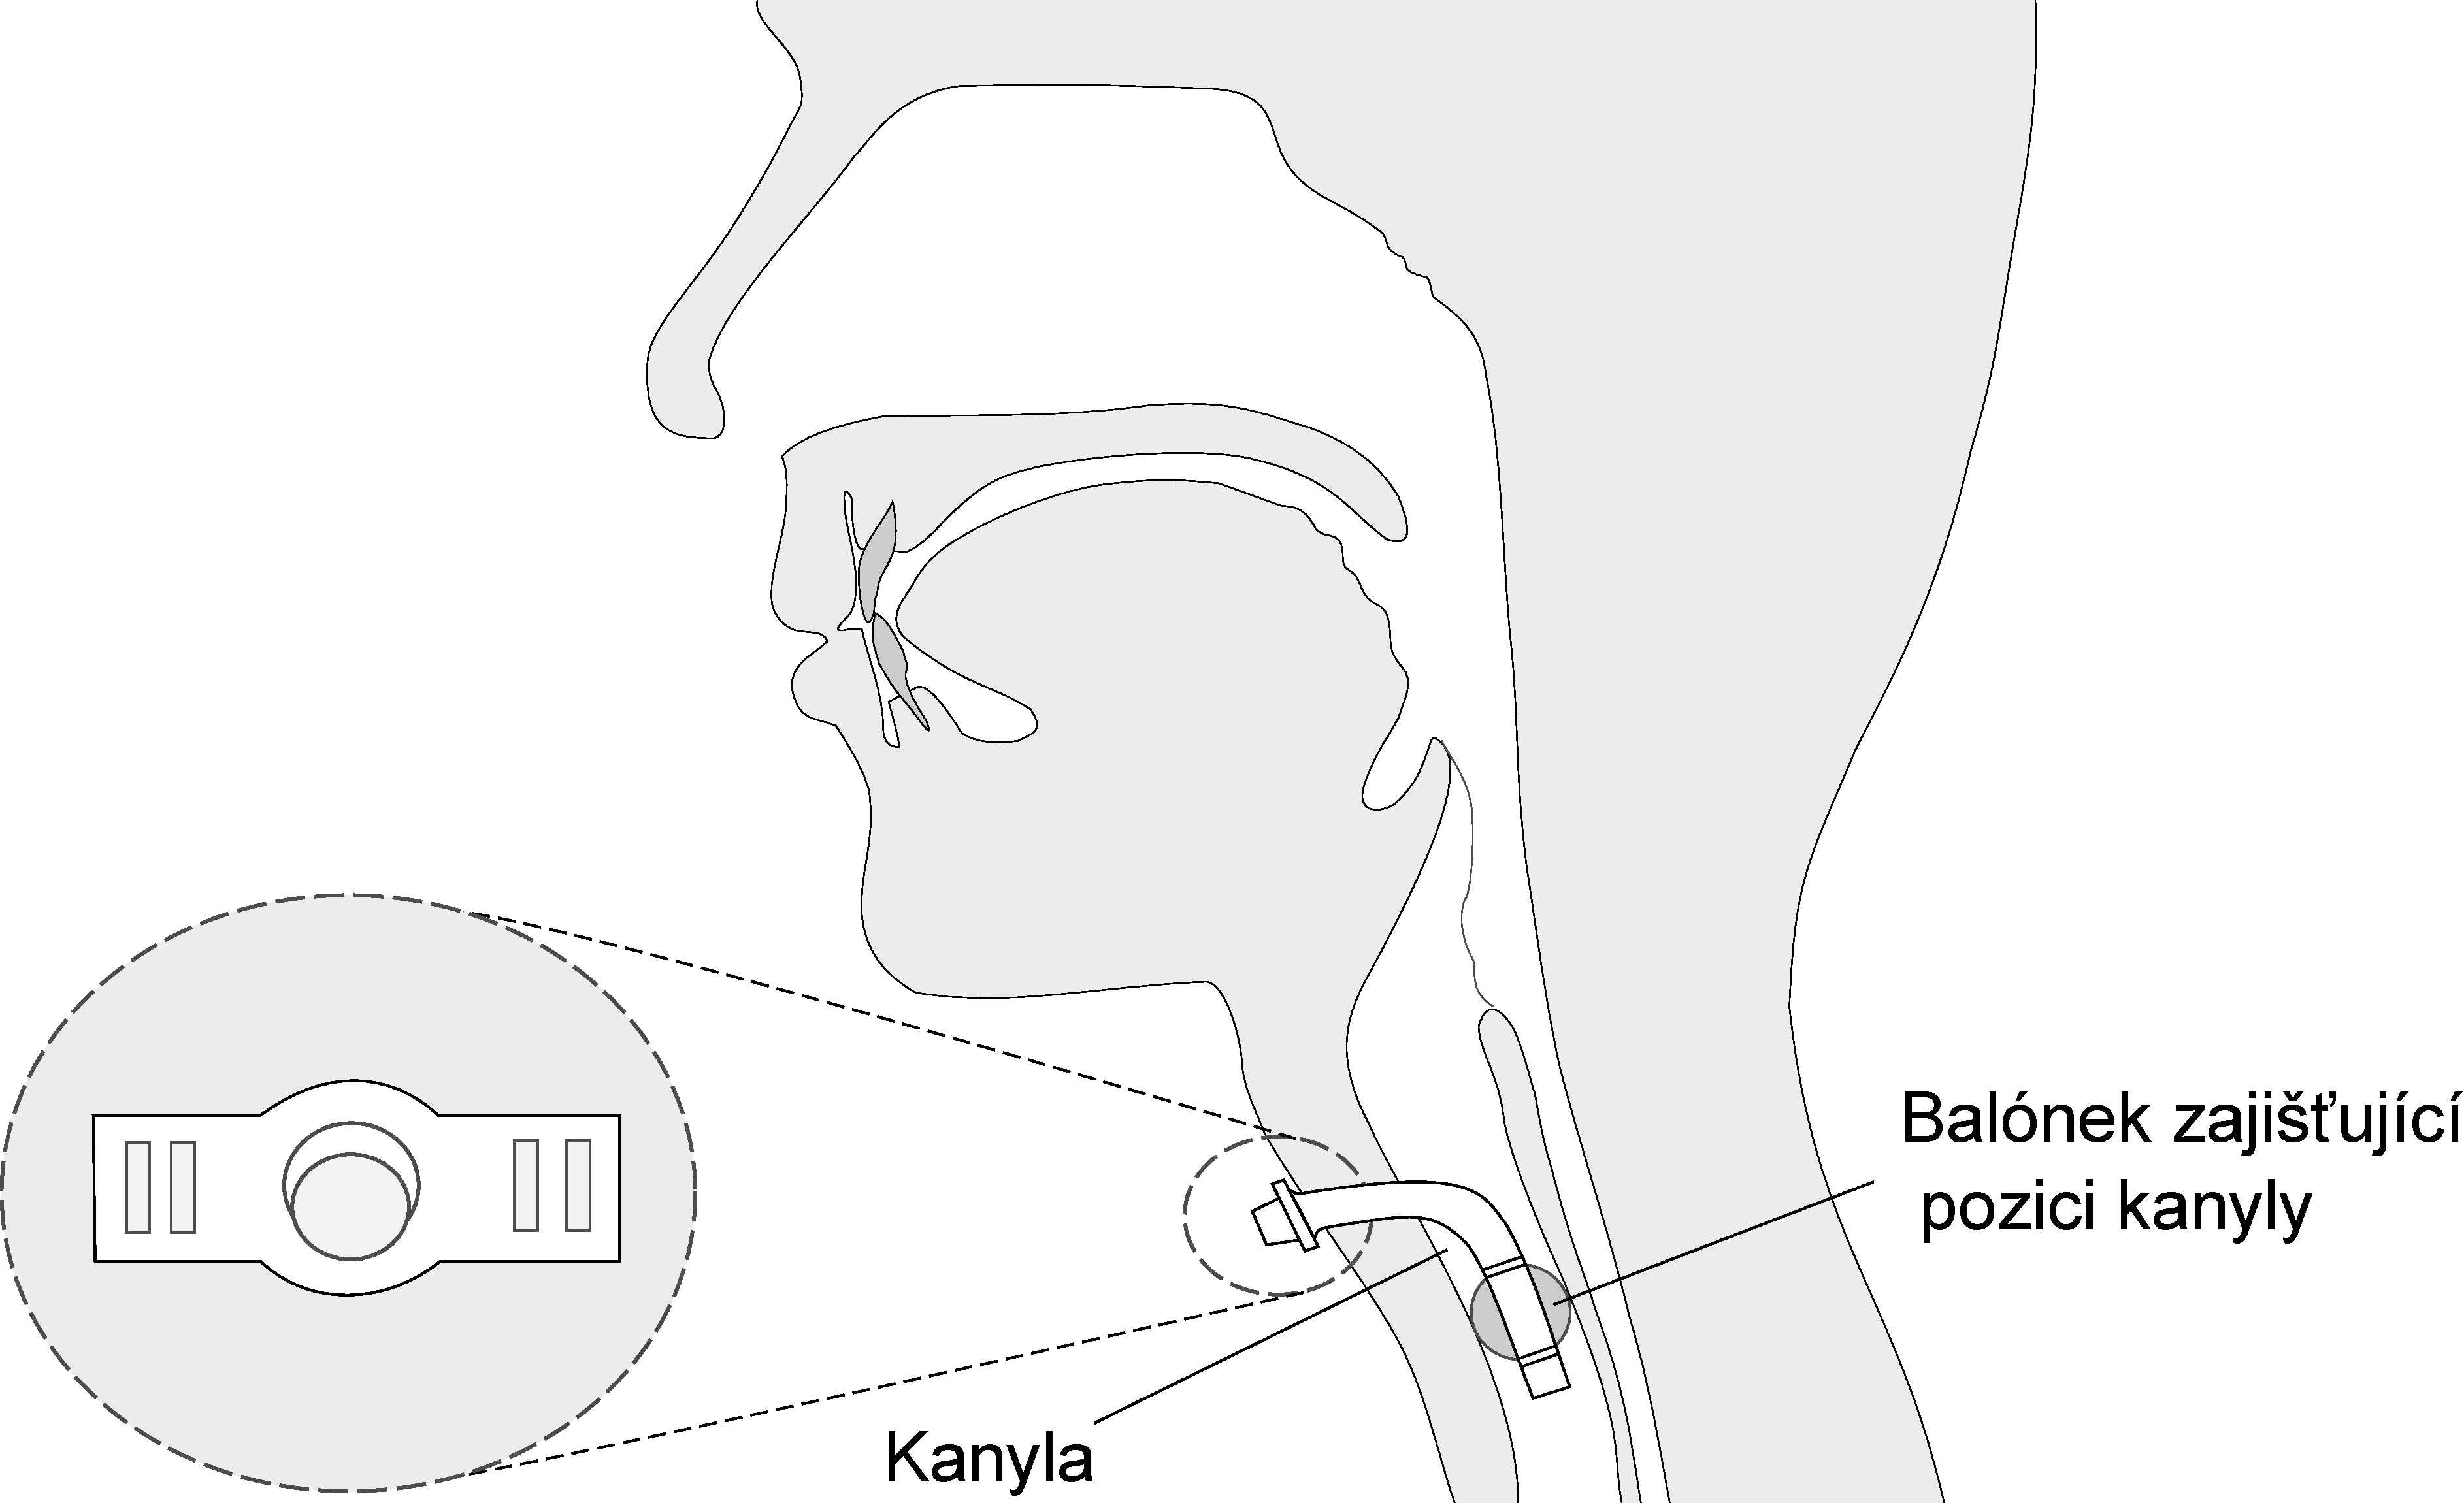
\includegraphics[width=0.9\linewidth]{ch3-cause/figures/tracheostomie}
    \caption[Tracheostomie]{Tracheostomie}
    \label{fig:cause:desease:tracheostomy}
  \end{center}
\end{figure}

Další významnou metodou využívanou k léčbě nádorových onemocnění představuje
\textbf{aktinoterapie} neboli léčba ozařováním. Podstatou postupu je
periodické vystavování buňky ionizujícímu záření. Energie z tohoto záření je
předávána buňce, která je tím poškozována. Tento postup se opírá o předpoklad,
že nádorové buňky jsou náchylnější k poškození. Záření ovšem ovlivňuje i
zdravé buňky, a proto je tato léčba pro organismus velkou zátěží.
Aktinoterapie je možné využít jednak u případů, kdy je cílem terapie úplné
vyléčení, tak i v případech, kdy naprosté odstranění onemocnění není možné. V
druhém případě je metoda využívána k prodloužení a zkvalitnění života
\cite{Slavicek2000}.

Aktinoterapii je možné využít jako hlavní léčebnou metodu (primární
aktinoterapie) nebo i ve spojení s ostatními metodami. V případě primární se k
léčbě využívá pouze ozařování a cílem je úplné odstranění všech defektních
buněk. Z podstaty metody, zejména dopadů léčby na lidský organismus, je
zřejmé, že tímto způsobem je ve většině případů možno léčit pouze malé nádory.

Ve spojení s chirurgickou léčbou rozlišujeme předoperační, pooperační nebo
tzv. sandwich (tj. před a po chirurgickém zákroku) aktinoterapii. Předoperační
ozařování je užíváno v případech, kdy není možné původní nádor vyoperovat.
Cílem je zmenšení tumoru do takové míry, aby jej bylo možné chirurgicky
odstranit. Někdy je předoperační ozařování spojeno s chemoterapií.
U pooperační aktinoterapie je záměrem odstranění potencionálních
mikroskopických zbytků tumoru, které by mohly znovu začít růst.

Velmi často se ve spojení s léčbou rakoviny mluví i o proceduře zvané
\textbf{chemoterapie}. Podstatou je podávání léků zastavujících buněčné
dělení, tzv. cytostatik. Zjednodušeně řečeno se jedná o velmi toxický koktejl
látek sloužící k zahubení buňky tím, že poškodí určitou její část a zastaví
tak proces dělení. Na tuto léčbu jsou citlivé převážně rychle se dělící buňky.
Právě defektní buňky v tumoru mají obvykle určitým způsobem poškozeny opravné
mechanizmy a cytostatiky zasažená rakovinná buňka tak s větší pravděpodobností
zahyne. Samozřejmě nelze u chemoterapie hovořit o přesně zacílené léčbě.
Cytostatika postihují všechny buňky v lidském těle, a proto je možná namístě
srovnání s kobercovým bombardováním. S aplikací cytostatik je tak
spojena celá řada vedlejších rizik. Mezi nejzávažnější patří poškození ledvin
nebo poškození krvetvorby.

% \footnote{Při kobercovém bombardování
% dochází při ničení konkrétního cíle, ke zničení rozlehlé oblasti území. K
% prvnímu použití došlo ve Španělské občanské válce v roce 1937 a k hlavnímu
% rozmachu došlo v průběhu 2. světové války.}

Z výše uvedeného je zřejmé, že postižená osoba má velkou šanci na kompletní
vyléčení. V mnoha případech má však pacient trvalé následky (trvalá ztráta
hlasu) z~důvodu podcenění prvotních příznaků vážného onemocnění.

% subsubsection léčba_nádorového_onemocnění (end)

% subsection rakovina_hrtanu (end)

%!TEX root = ../thesis.tex
\section{Rehabilitace hlasu po totální laryngektomii}
\label{sec:cause:treatment}

Nesporná výhoda totální laryngektomie neoddiskutovatelně spočívá v likvidaci
primárního nádorového onemocnění. Následky operace však s sebou nesou obrovský
zásah do kvality života pacienta. Okem nejviditelnější změnu představuje
přítomnost tracheostomie a s ní spojený způsob dýchání. Tato skutečnost má
spoustu, na první pohled ne úplně očividných, následků. Postižený člověk
ztrácí přirozené zvlhčování, ohřev a filtraci vdechovaného vzduchu, jež má za
následek vyšší náchylnost k~respiračním onemocněním. Příčina spočívá v
průchodu vzduchu do průdušnice přes tracheostomii a nikoli přes nosní dutiny.

Pro samotného pacienta je však nejspíše nejobtížnější se vypořádat s trvalou
ztrátou vlastního hlasu. Z tohoto důvodu se již samotný autor procedury doktor
Billroth zaobíral otázkou rehabilitace hlasu. Jeho první pokusy s kovovou
tracheostomickou kanylou sice umožňovaly pacientovi hovořit, ale svou
konstrukcí pacienta spíše ohrožovaly na životě \cite{Kramp2009}. Proto se více
uchytila metoda tzv. jícnového hlasu \cite{Sebova-Sedenkova2006}. Ve stejnou
dobu, tedy přibližně začátkem minulého století, se začaly objevovat první
interní a externí hlasové aparáty. V současnosti je rehabilitace hlasu možná
pomocí:

\begin{itemize}
  \item \textbf{foniatrických metod}, mezi které patří jícnový hlas a elektrolarynx,
  \item \textbf{chirurgicko-protetickým způsobem}, který spočívá ve vytvoření kanálku skrze stěnu mezi průdušnicí a jícnem,
  \item \textbf{vytvoření hrtanu podobných struktur chirurgickým způsobem},
  \item \textbf{transplantace hrtanu}.
\end{itemize}

Z uvedeného výčtu se může zdát, že máme k dispozici relativně širokou škálu
možností, jak pacientovi vrátit schopnost vyjadřování pomocí mluvené řeči.
Ovšem je nutné si uvědomit, že je potřeba volit konkrétní metodu podle stavu a
možností pacienta. Jinými slovy, ne každá metoda se hodí pro každého pacienta
a žádná z~metod není univerzální pro všechny pacienty.

\subsection{Foniatrické metody} % (fold)
\label{sub:cause:treatment:foniatric}

Ačkoli odstranění hrtanu vyústí ve ztrátu hlasu, neznamená to, že by byla
úplně eliminována schopnost produkovat řeč. V procesu vytváření hlasu zastává
odstraněný orgán pouze (i když velmi zásadní) roli generátoru zvuku. Zbylé
orgány (hrdelní, nosní a ústní dutina a další) zůstávají nedotčeny a mohou i
nadále plnit svou funkci. Logicky se tak nabízí myšlenka nahradit chybějící
zdroj zvuku jiným. Mezi nejpoužívanější metody patří jícnový hlas a
elektrolarynx.

\subsubsection{Jícnový hlas} % (fold)
\label{ssub:cause:treatment:foniatric:esophageal}

Počátek této metody se datuje do roku 1922, kdy si prof. MUDr. Miloslav Seeman
\cite{seeman1922speech} uvědomil, že funkci štěrbiny mezi hlasivkami (rima
glottidis) přebírá tzv. pseudoglottis, která se vytváří na úrovni horního
jícnového svěrače. Zároveň vypracoval a popsal metodiku vytváření jícnového
hlasu, při které se vzduch neplní do plic, ale do jícnu. Tato metoda se nazývá
\textbf{aspirační}. Princip spočívá v aktivním otevření jícnového svěrače,
nasáváním a vtlačováním vzduchu do jícnu pomocí polykání. Naplněním jícnu
vzduchem si pacient připravuje potřebný vzduch k následné
eruktaci\footnote{eruktace - latinsky název pro proces říhání (popřípadě
krkání), při kterém dochází k úniku plynů pocházejících ze žaludku dutinou
ústní.} vzduchu a produkci řeči. Vlastní jícnový hlas poté vzniká na přechodu
jícnu a hypofaryngu (spodní část hltanu). V této oblasti horního jícnového
zúžení dochází k rozkmitání sliznice a podslizniční vrstvy a produkci zvuku,
který je následně modulován stejně jako v případě přirozené produkce řeči.
Princip tvorby \uv{základního} tónu jícnového hlasu je znázorněn na obr.
\ref{fig:cause:treatment:esophageal}.

\begin{figure}[htb]
  \begin{center}
    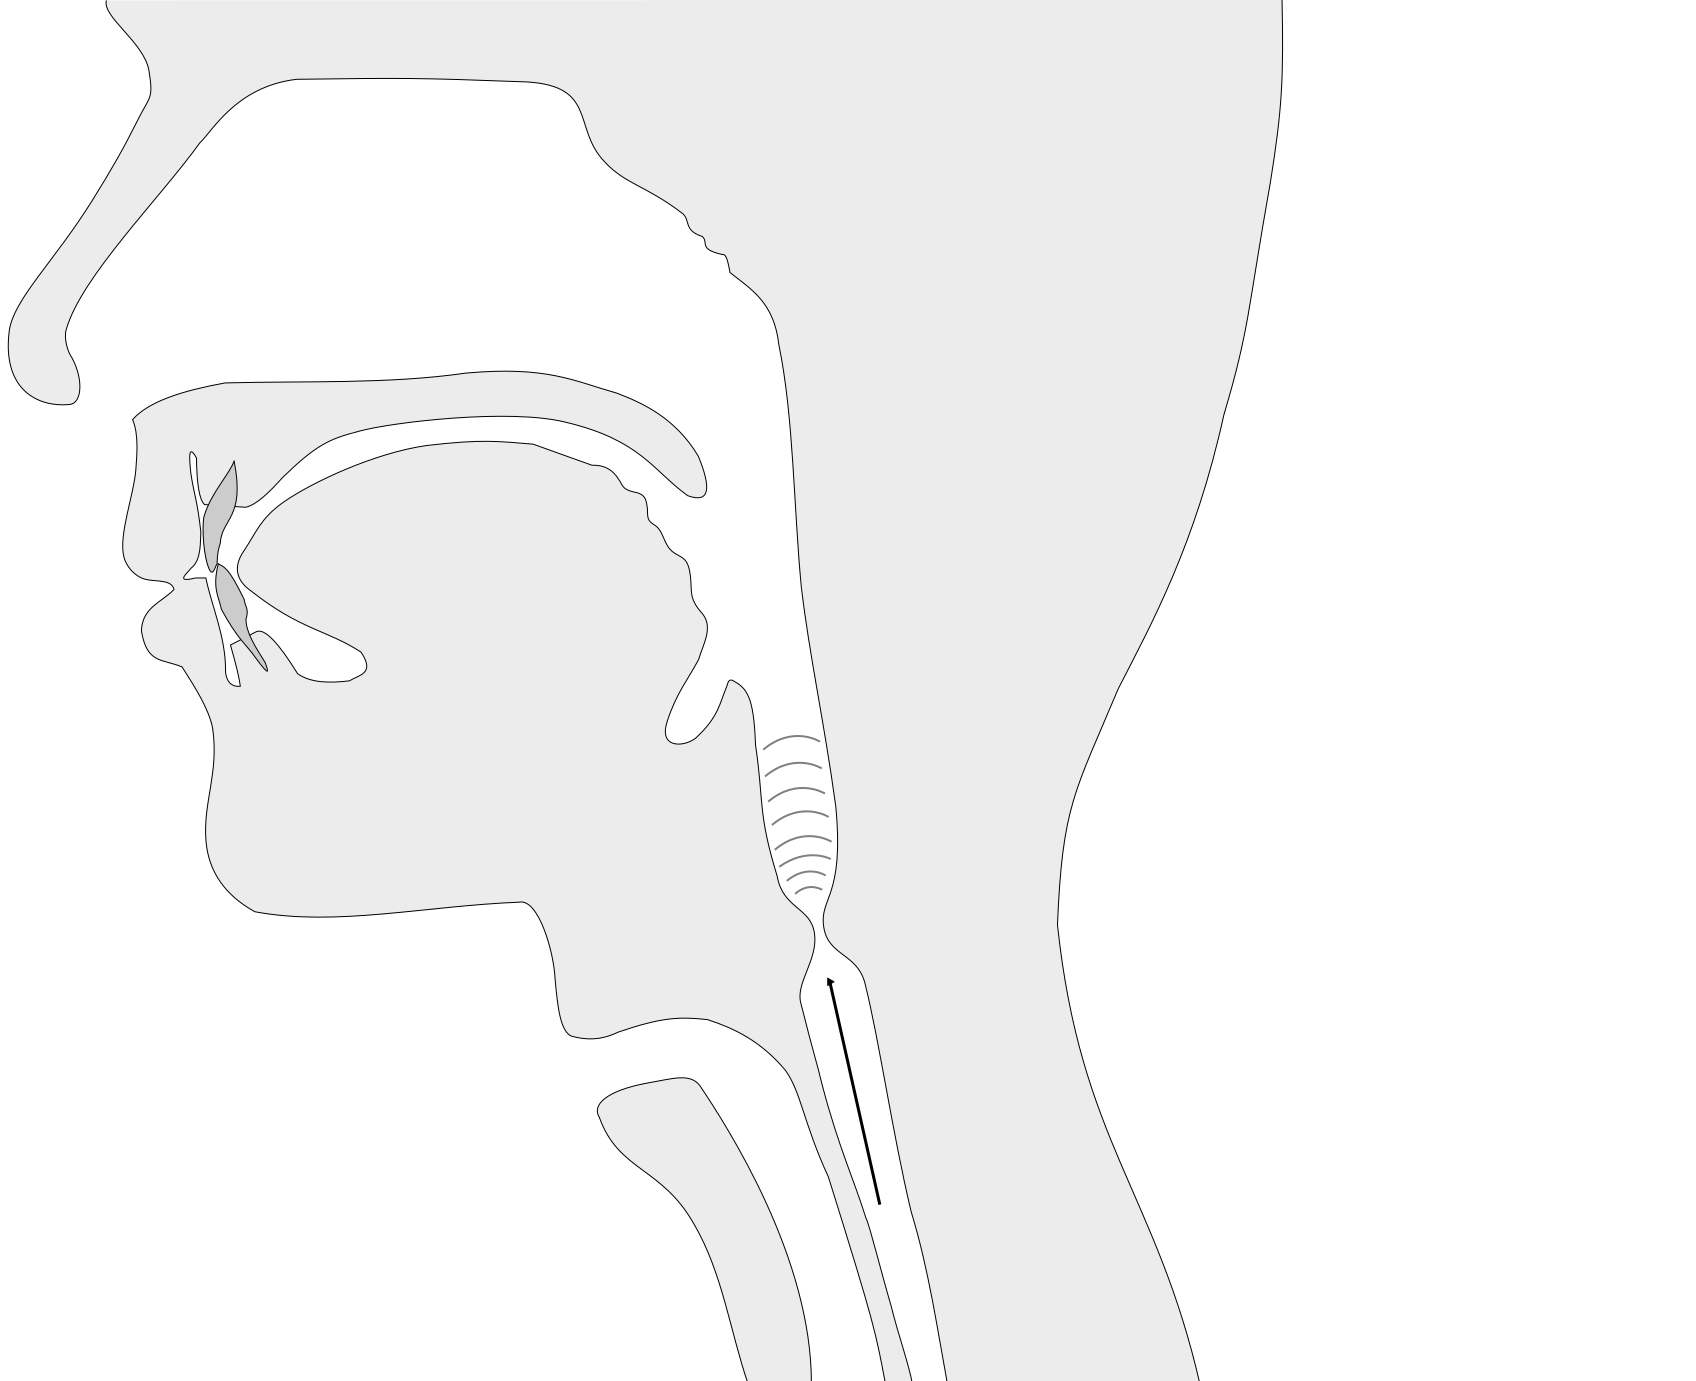
\includegraphics[width=0.6\linewidth]{ch2-cause/figures/esophageal}
    \caption[Princip tvorby jícnového hlasu]{Princip tvorby jícnového hlasu. Průchodem vzduchu přes zúžení vzniká základní tón jícnového hlasu.}
    \label{fig:cause:treatment:esophageal}
  \end{center}
\end{figure}

Kromě aspirační metody je ještě možné se setkat s metodou \textbf{injekční}.
Hlavní rozdíl spočívá v principu plnění vzduchu do jícnu. Při aspirační metodě
se využívá polykání, zatímco v tomto případě je využito kořene jazyka, kterým
je vzduch vtlačován do jícnu. Následný princip produkce hlasu je již shodný s
původní metodou. S tímto principem se můžeme setkat u pacientů, kterým byla
při laryngektomii odstraněna jazylka a aspirační náplň není možná.

Proces učení jícnového hlasu by měl začít co možná nejdříve po operaci. Pokud
je to možné, tak se s výukou začíná ještě za pobytu pacienta na ORL klinice
nebo krátce po propuštění. V první fázi se pacient učí pouze slabiky
sestávající z explosivy a souhlásky. Postupně se však přidávají slabičné
shluky, které sice nedávají smysl, ale pomáhají v osvojení potřebné techniky.
V případě úspěšného zvládnutí se přistupuje k nácviku frází a souvislé řeči.
Potřebnou dobu k nácviku jícnového hlasu nelze přesně určit, protože je
závislá na mnoha faktorech. V literatuře se uvádí, že je potřeba 30 až 50
hodin velmi intenzivního tréninku k osvojení jícnového hlasu.

Míra úspěšnosti nácviku srozumitelného hlasu se uvádí v rozsahu od 14\% do
75\%. Takto obrovský rozsah značí o mnoha faktorech, které mohou ovlivnit
úspěšné osvojení jícnového hlasu. Mezi možné příčiny neúspěchu patří
fyziologické nebo anatomické problémy, psychologické problémy, nebo jednoduše
neadekvátní podpora při řečové terapii \cite{Brown2003}. Velkou roli také
hraje snaha a odhodlání samotného pacienta.

Nepopíratelnou výhodou této techniky rehabilitace je nezávislost pacienta na
lékaři po úspěšném osvojení jícnového hlasu a permanentní oddělení dýchacích a
polykacích cest bez rizika vniknutí potravy do dýchacích cest. Mezi nesporné
výhody také patří volné ruce při vytváření řeči. Za nevýhody se obecně
považuje srozumitelnost produkovaného hlasu. Je to způsobeno jednak
\uv{břišním} zabarvením, které je už z podstaty metody přítomné, a dále také
nízkou intenzitou a krátkou výdrží při tvorbě tónu. Za negativum se dá také
považovat množství pacientem vynaloženého úsilí potřebného k osvojení
techniky. Velmi často se také mluvčí ostýchají jícnový hlas používat, protože
mají pocit, že je společensky nevhodné dorozumívat se formou blízkou říhání. Z
tohoto důvodu se odhaduje, že v běžném životě využívá jícnový hlas pouze 20 až
30\% pacientů, kteří se začali tuto techniku učit \cite{Hradecka2007}.

% subsubsection jícnový_hlas (end)

\subsubsection{Elektrolarynx} % (fold)
\label{ssub:cause:treatment:foniatric:elektrolarynx}

Rehabilitace hlasu pomocí elektrolarynxu se řadí mezi tzv. elektromechanické
metody. Princip spočívá v přikládání zařízení, které obsahuje generátor zvuku
nazývaný elektrolarynx. Přiložením do oblasti spodiny úst a aktivací zařízení
se generovaný zvuk a vibrace přenášejí do dutiny ústní a dalších přilehlých
artikulačních orgánů. Následnou artikulací je pacient schopen hovořit.
Znázorněno na obr. \ref{fig:cause:treatment:electrolarynx}.

\begin{figure}[htb]
  \begin{center}
    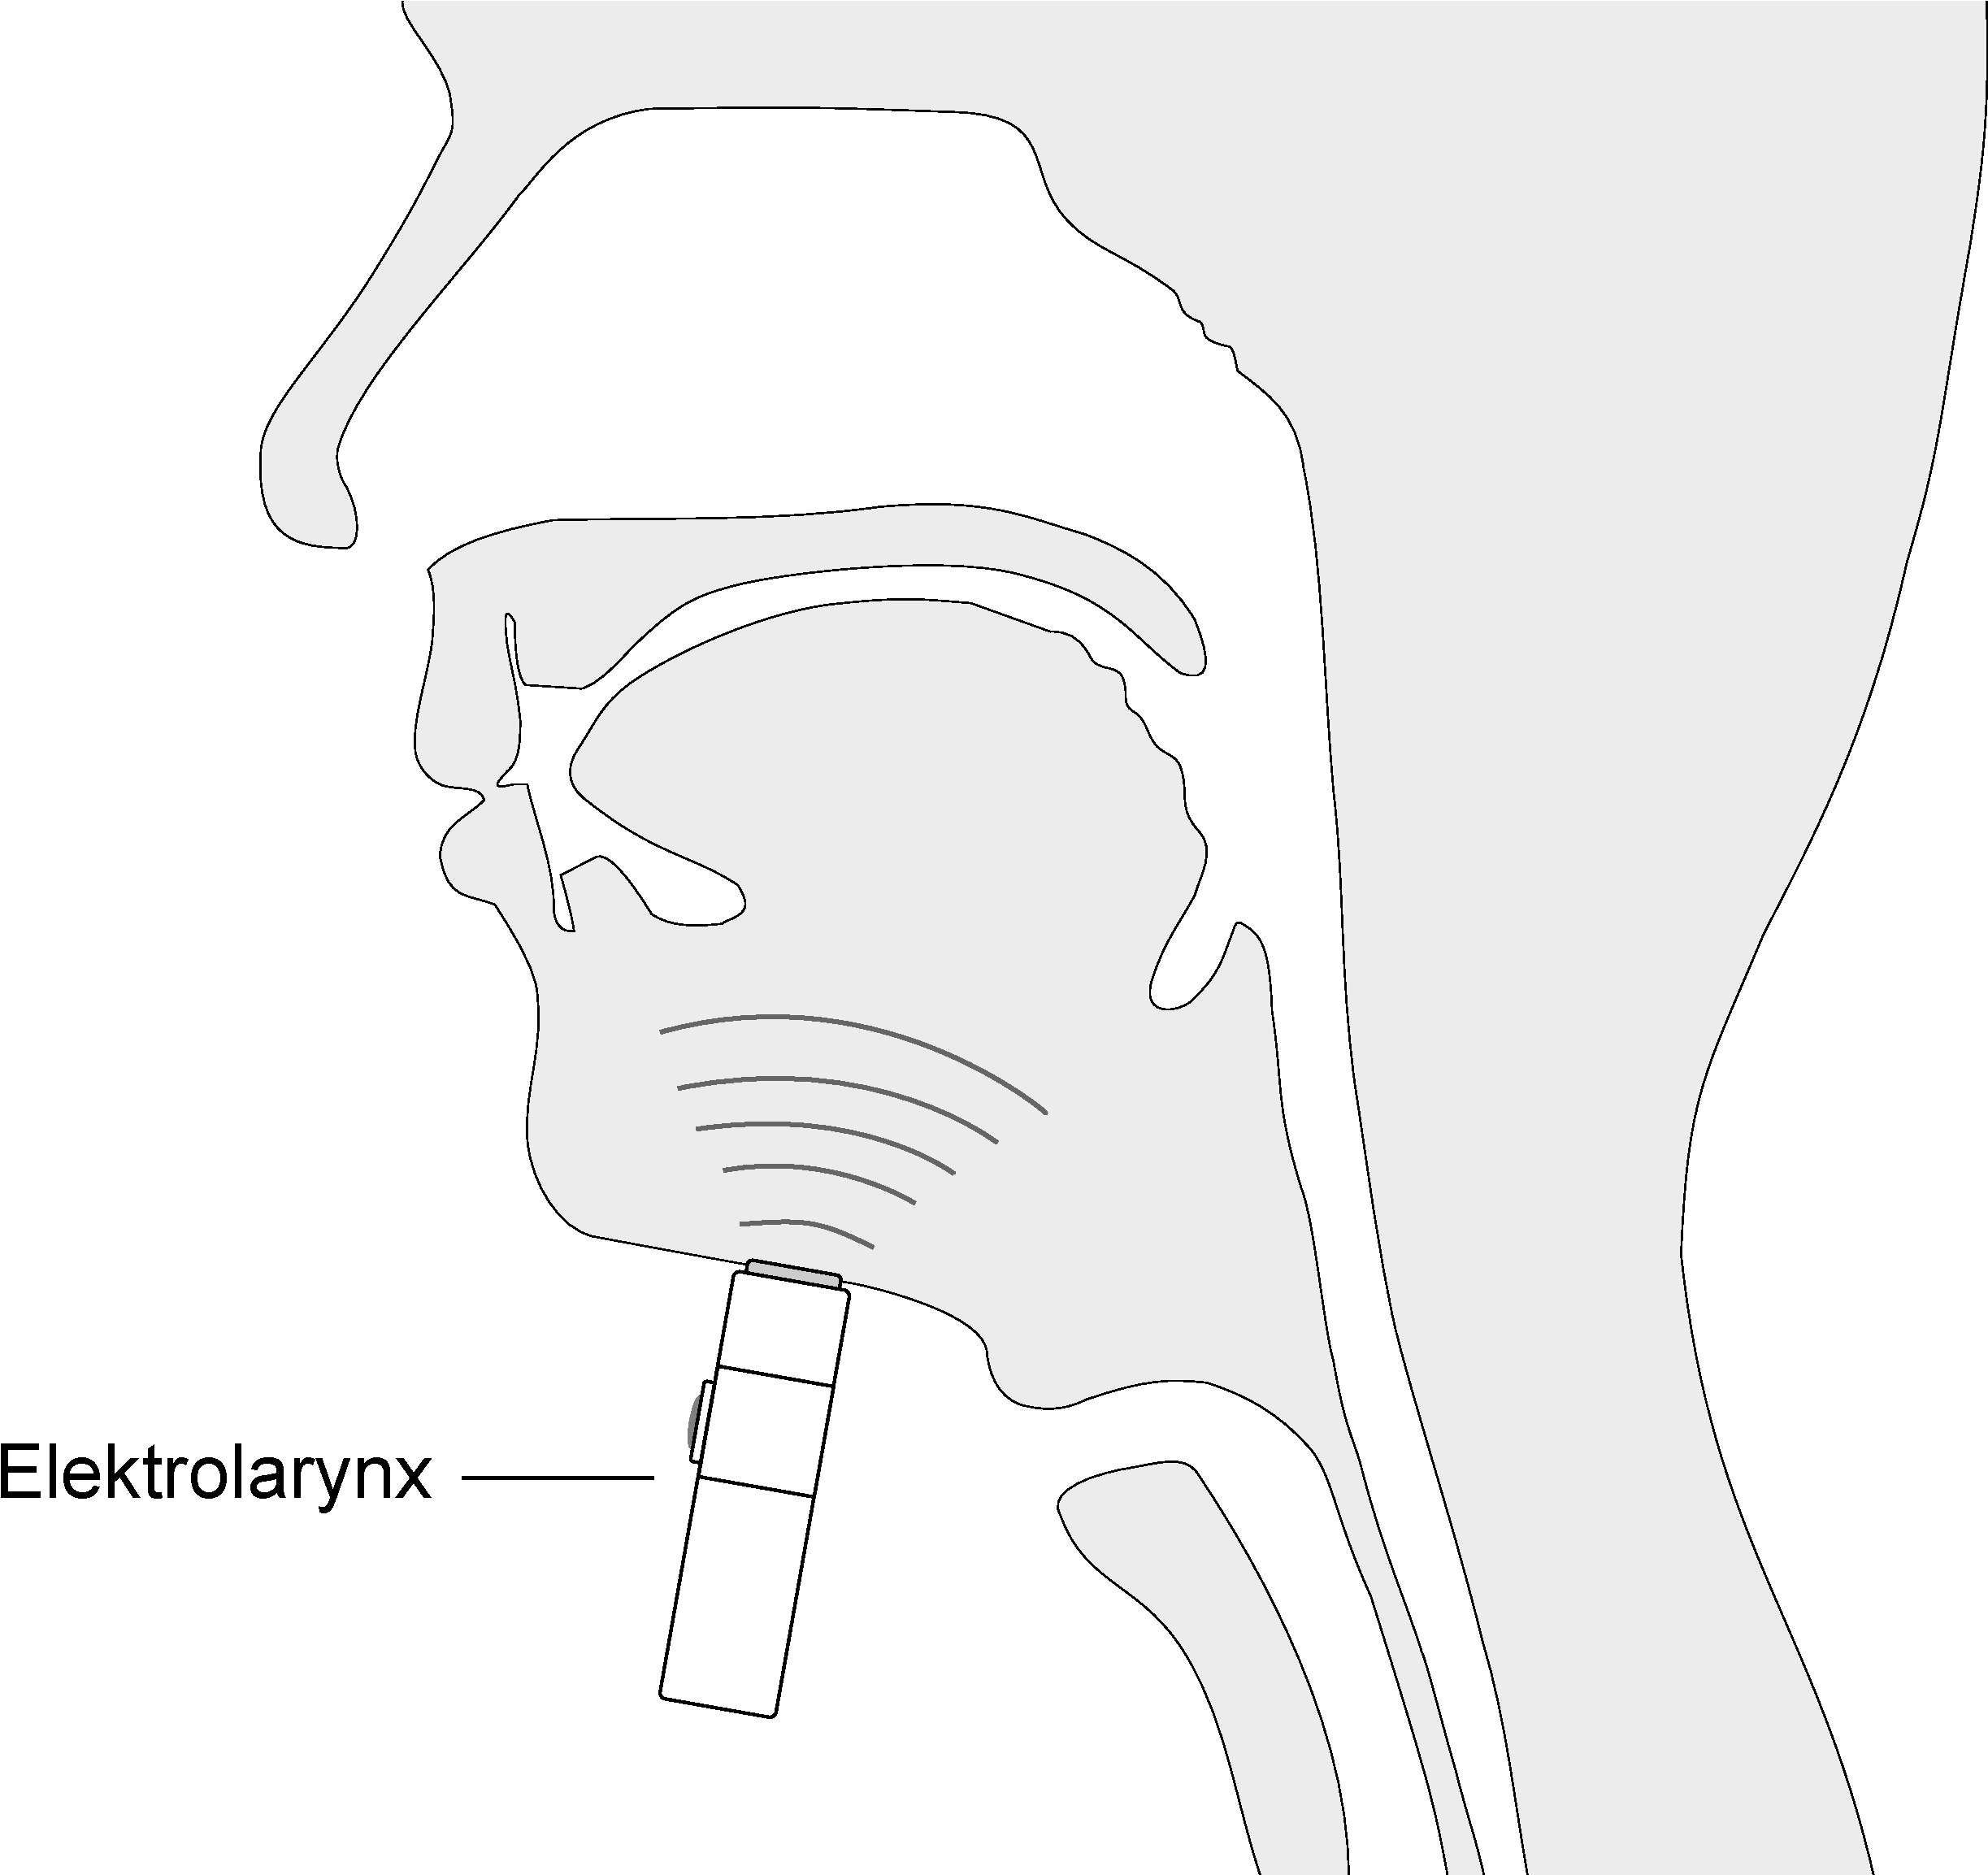
\includegraphics[width=0.6\linewidth]{ch2-cause/figures/electrolarynx}
    \caption[Princip rehabilitace hlasu pomocí elektrolarynxu]{Princip rehabilitace hlasu pomocí elektrolarynxu.}
    \label{fig:cause:treatment:electrolarynx}
  \end{center}
\end{figure}

% TODO: ELEKTROLARYNX pasaze o monotonosti reci poradne promyslet

Takto generovaná řeč se vyznačuje několika charakteristickými rysy. V první
řadě řeč budí velmi mechanický dojem. Důvodem je samozřejmě samotný
elektrolarynx, jelikož se jedná o elektromechanický generátor zvuku s
konstantním buzením, je také základní frekvence produkovaného hlasu více či
méně konstantní. Řečník tak má velmi omezené možnosti, jak řeč emotivně
zabarvovat. V průběhu času se objevily snahy průběžně měnit frekvenci zařízení
a tím ovlivňovat základní frekvenci produkované řeči \cite{Kikuchi2004,
Uemi1994, Goldstein2004}. Hlavním problém všech těchto zařízení je docílit
změnu fundamentální frekvence na základě toho, co chce řečník říci. V současné
době existují pouze experimentální zařízení, která umožňují ve velmi omezené
míře změnu frekvence \cite{Liu2007}. Další charakteristický rys představuje
nižší srozumitelnost řeči, která se ještě snižuje s~rostoucím okolním hlukem.
Velmi často se stává, že posluchač, který se s takto produkovanou řečí setkává
poprvé, není schopen plně porozumět. Se srozumitelností souvisí i další
charakteristický rys, kterým je přítomnost zvukového podkresu produkovaného
samotným přístrojem.

Za hlavní výhodu elektrolarynxu se považuje rychlost osvojení schopnosti
produkovat řeč. Zároveň je tato metoda vhodná pro téměř všechny pacienty
postižené ztrátou hlasu způsobenou léčbou karcinomu hrtanu. Z tohoto důvodu se
hojně užívá u pacientů, kteří si neosvojili jícnový hlas nebo u nich není
možné využití ostatních chirurgických metod.
Za nevýhody se obecně pokládá kvalita produkované řeči, tedy monotonní a
mechanicky znějící hlas. Dále potom zaměstnání jedné ruky držením nebo
spouštěním zařízení.

Samostatnou kapitolou může být psychologický dopad na pacienta. Stejně jako
u~jícnového hlasu se řeč produkovaná promocí elektrolarynxu jeví odlišně od
řeči přirozené. Navíc se ještě přidává potřeba využití nějakého zařízení.
Člověk proto v~mnoha případech cítí ostych a bojí se na veřejnosti mluvit.

% subsubsection elektrolarynx (end)

% subsection subsection_name (end)

\subsection{Chirurgicko-protetická metoda} % (fold)
\label{sub:cause:treatment:tracheo}

Další možnost rehabilitace hlasu představuje tracheoezofageální (zkr. TE) protéza.
První zmínka o vytvoření fistule\footnote{fistule (česky píštěl) je abnormální
otvor mezi dvěma dutými orgány, nebo mezi dutým orgánem a kůží.} mezi
průdušnicí a jícnem pochází z roku 1932. V~tomto roce doktor Guttman poprvé
vytvořil tracheoezofageání shunt\footnote{shunt - kanál, kterým je tekutina
odkloněna z přirozené dráhy. Tento kanál může být vytvořen chirurgicky nebo
pomocí syntetické trubice.} (\uv{umělá píštěl}). Hlavní myšlenka spočívá ve
vytvoření cesty prostřednictvím píštěle, pomocí které u tracheostomovaného
člověka může proudit vzduch z plic do úst. Za normálních okolností vzduch
proudí skrze tracheostomii a do úst se tak nedostane. Zacpe-li si pacient
stomu, může proud vzduchu proudit skrze píštěl do úst. Vzduch procházející
přes fistuli naráží do stěn jícnu a je rozvibrován. Tyto vibrace jsou následně
modulovány pomocí artikulačních ústrojí a tak vzniká řeč.
Tento ojedinělý zákrok otevřel cestu k chirurgické hlasové rehabilitaci.
Vzniklo několik operačních metod, které se navzájem lišili víceméně jen
umístěním fistule \cite{Kramp2009}.

Hlavní snahou chirurgů bylo vytvoření bezpečné, správně nasměrované píštěle
umožňující tvorbu hlasu. Bohužel v mnoha případech byly tyto zákroky spojené
s~vážnými komplikacemi (infekce, zápaly či těžká krvácení). Důležitým
problémem, se kterým se jednotlivý tvůrci museli vypořádat, byla stálost
vytvořeného otvoru tak, aby jím neprotékaly tekutiny špatným směrem a
nedocházelo k zatékání do dýchacích cest a orgánů. Jelikož se jednalo o velmi
náročné techniky, a bylo s nimi spojeno velké množství rizik, došlo v
80.letech 20.století k opadnutí snah tyto metody aplikovat.

Svou renesanci zažily s vložením jednocestného ventilu, který umožňoval pouze
jednosměrný průchod tekutin skrze píštěl, jak je ilustrováno na obr.
\ref{fig:cause:treatment:shunt}. První komerčně dostupná protéza se objevila
v~80.letech 20.století v USA. Na obr. \ref{fig:cause:treatment:prosthesis} jsou
zobrazeny příklady různých typů protéz. Na používané protézy jsou kladené
přísné nároky a musí vyhovovat určitým požadavkům. Předně se musí vyrábět
z~biokompatibilního materiálu, který odolává biodegradaci. Tím je zaručena
dlouhodobá trvanlivost a správná funkce. Potřebný tlak k otevření
faryngoezofageálního segmentu by měl být co nejnižší, aby bylo možné vytvářet
plynulou řeč. První vyráběné protézy měly tento tlak příliš vysoký a omezovaly
tak množinu potencionálních pacientů. Nejmodernější protézy se již vyznačují
velmi nízkým otevíracím fonačním tlakem. V~neposlední řadě by měla být protéza
samofixační a snadno vyměnitelná.

\begin{figure}[htb]
  \begin{center}
    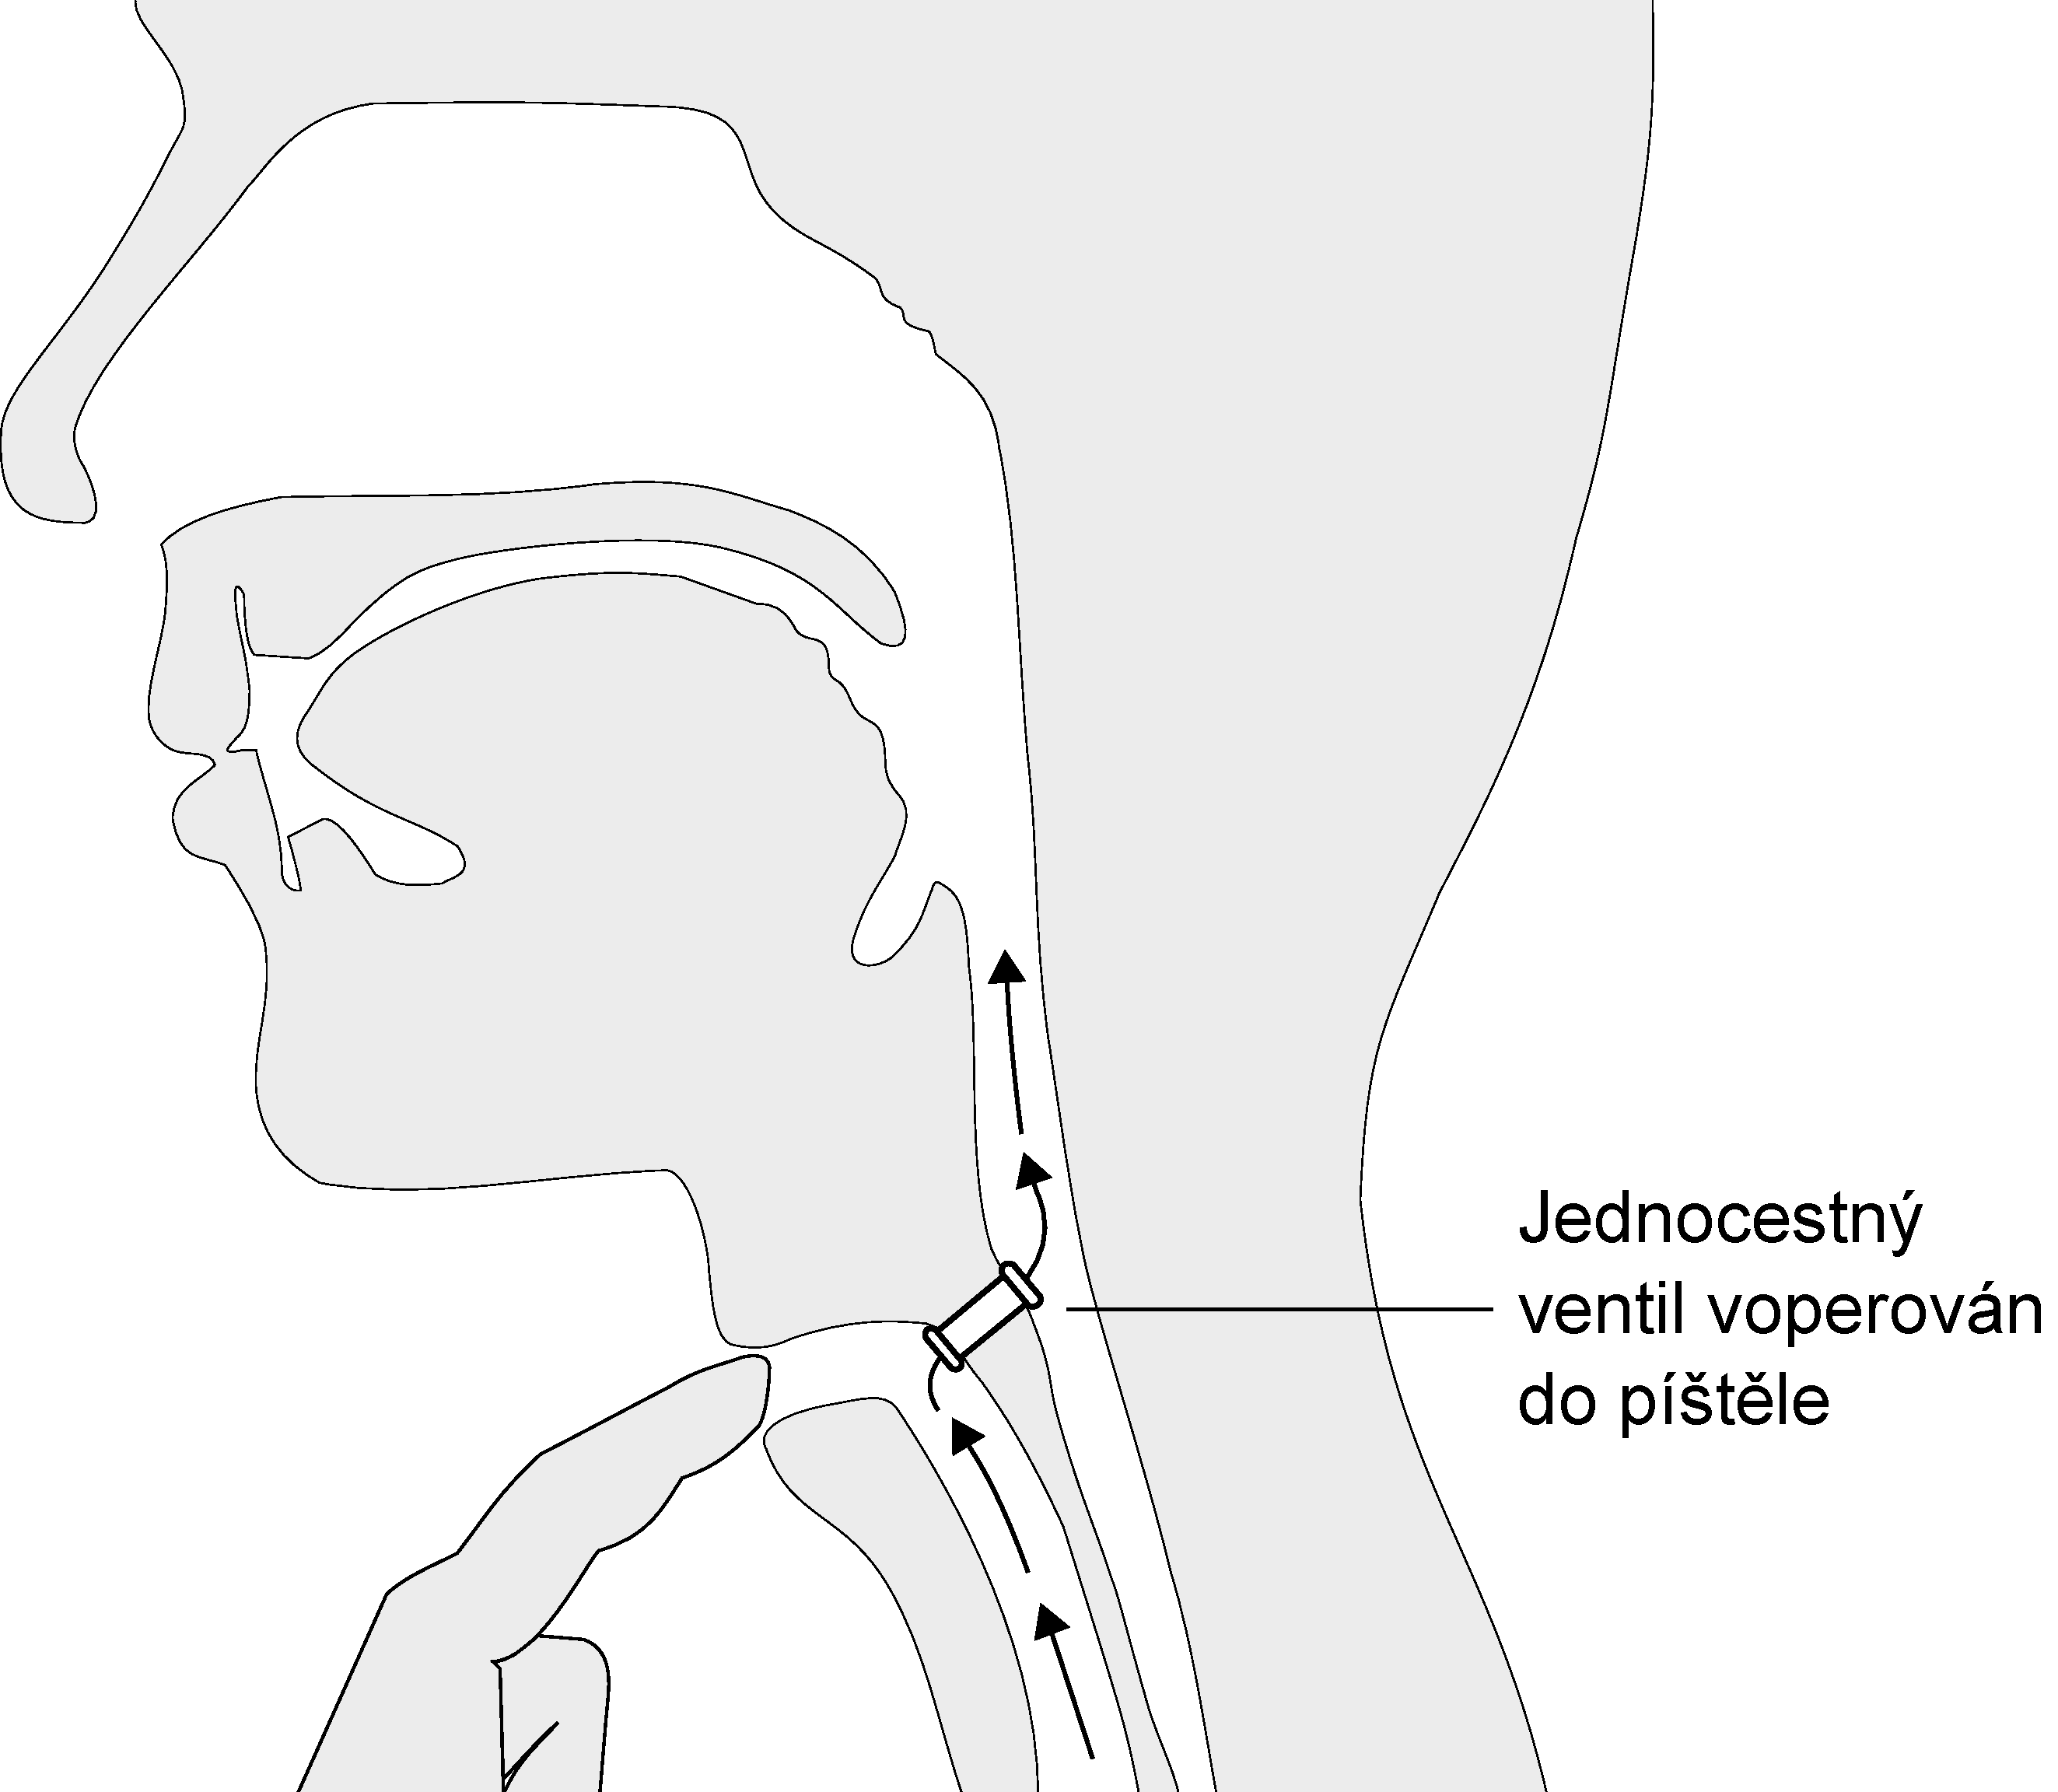
\includegraphics[width=0.6\linewidth]{ch2-cause/figures/te-shunt}
    \caption[Průchod vzduchu tracheoezofageální protézou]{Průchod vzduchu tracheoezofageální protézou.}
    \label{fig:cause:treatment:shunt}
  \end{center}
\end{figure}

\begin{figure}[htb]
  \begin{center}
    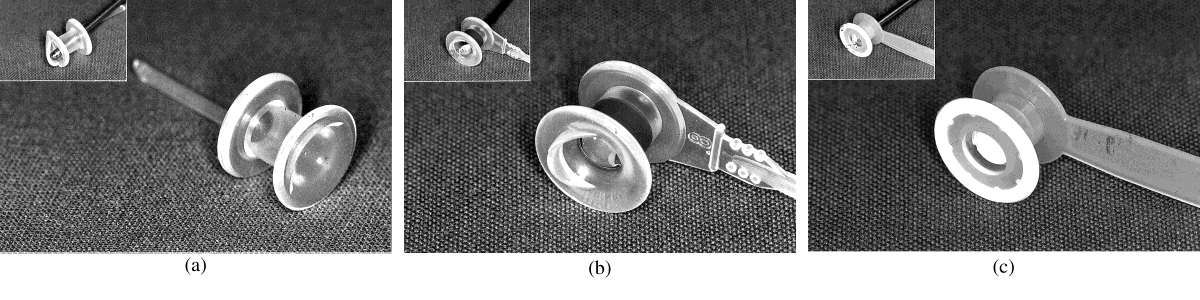
\includegraphics[width=0.9\linewidth]{ch2-cause/figures/te-protezy}
    \caption[Ilustrace používaných TE protéz]{Ilustrace používaných TE protéz (a) Gronigenova nízkotlaká protéza, (b) Provox2 a (c) Blom-Singer protéza.}
    \label{fig:cause:treatment:prosthesis}
  \end{center}
\end{figure}

V praxi se používá několik druhů protéz. Hlavním rozdílem mezi nimi však je
zda se pacient přímo účastní výměny ventilu, jehož fundamentální funkcí je
vytvoření průchodu pro vzduch proudící z průdušnice do jícnu. U protéz, které
jsou vyměňovány operačně, se doba používání pohybuje od 3 do 6 měsíců. Tento
interval velmi významně ovlivňuje tvorba biofilmu na povrchu náhrady. K tvorbě
dochází následkem přímého kontaktu protézy s tělními tekutinami a potravou.
Rychlost tvorby biofilmu ovlivňuje tvar a materiál, ze kterého je náhrada
vytvořena \cite{Leunisse2001}. U typů, které si nositel může měnit sám, se
předpokládá, že budou čištěny nebo měněny přibližně jednou za dva týdny.

Samotný zákrok zavedení protézy je možné provést zároveň s výkonem totální
laryngektomie (tzv. primární zavedení hlasové protézy) nebo až po zotavení
pacienta z~náročné léčby nádorového onemocnění (tzv. sekundární zavedení).
Primární zavedení umožňuje začít s hlasovou rehabilitací krátce po odstranění
hrtanu. Zároveň pacient nemusí v krátké době podstupovat druhou operaci, při
které by se vkládal jednocestný ventil do vytvořené fistule.

V praxi se ukázalo, že úspěšnost rehabilitace je více než 80\%
\cite{Slavicek2002}. Důležitým faktorem, stejně jako u jícnového hlasu, je
funkčnost faryngoezofageálního segmentu. Dále také otvírací tlak horního
jícnového svěrače. Hlas tvořený protézou se vyznačuje vysokou kvalitou, dobrou
srozumitelností, individuálním zabarvením a relativně dlouhou fonační dobou
dosahující průměrně 20 sekund \cite{Saito2003}. Oproti jícnovému hlasu není potřeba
tak intenzivní edukace pacienta k plnému osvojení hlasu. V současnosti se
jedná o nejpoužívanější metodu rehabilitace hlasu.

% TODO: Vyhody nevyhody metody - film tvorici se na proteze
% TODO: Kriteria na pacienta


% subsection chirurgicko_protetická_metoda (end)

\subsection{Hrtanu podobné struktury} % (fold)
\label{sub:cause:tratment:structure}

S rozvojem mikrovaskulárních\footnote{mikrovaskulární - část oběhového systému
složeného z nejmenších cév, jako jsou kapiláry, žilky aj.} transplantátů se
začaly objevovat postupy, které umožňovaly rehabilitovat hlas pouze pomocí
chirurgického zákroku. Tyto techniky umožňují permanentní spojení hypofaryngu
s tracheou pomocí vlastní tkáně pacienta.

První takovouto  metodu představil v roce 1984 doktor Ehrenberger
\cite{Kramp2009}, který popsal tzv. \uv{\textbf{řečový sifón}} (angl. \textbf{speech
siphon}). Tento sifón je vytvořen z části tenkého střeva zvané lačník
(jejunum). Spojení mezi hrtanem a hltanem je dvakrát esovitě zahnuto tak, aby
bylo minimalizováno riziko sekundární aspirace. Schéma \uv{řečového sifónu}
podle Ehrenberga je znázorněno na obr. \ref{fig:cause:treatment:microvascular}
A. Již na první pohled je zřejmé, že se jedná o velmi náročný chirurgický
zákrok. První články publikované autorským kolektivem prezentovaly velmi dobré
funkční výsledky metody. Podle \cite {Sebova-Sedenkova2006} bylo doposud
operováno přibližně 60 pacientů.

V roce 1990 byla popsána laryngoplastika podle Hagena. V tomto případě se
vytváří tzv. \textbf{neolarynx}, k jehož vytvoření se používá štěp z
předloktí. Vnitřek neolaryngu je kryt kůží. Neoglottis je vyztužen chrupavkou
a překrývá vchod do neolaryngu tak, aby nedocházelo k sekundární aspiraci.
Laryngoplastika podle Hagena je znázorněna na obr.
\ref{fig:cause:treatment:microvascular} B. Doposud bylo operováno přibližně 300
pacientů \cite{Sebova-Sedenkova2006}.

\begin{figure}[htb]
  \begin{center}
    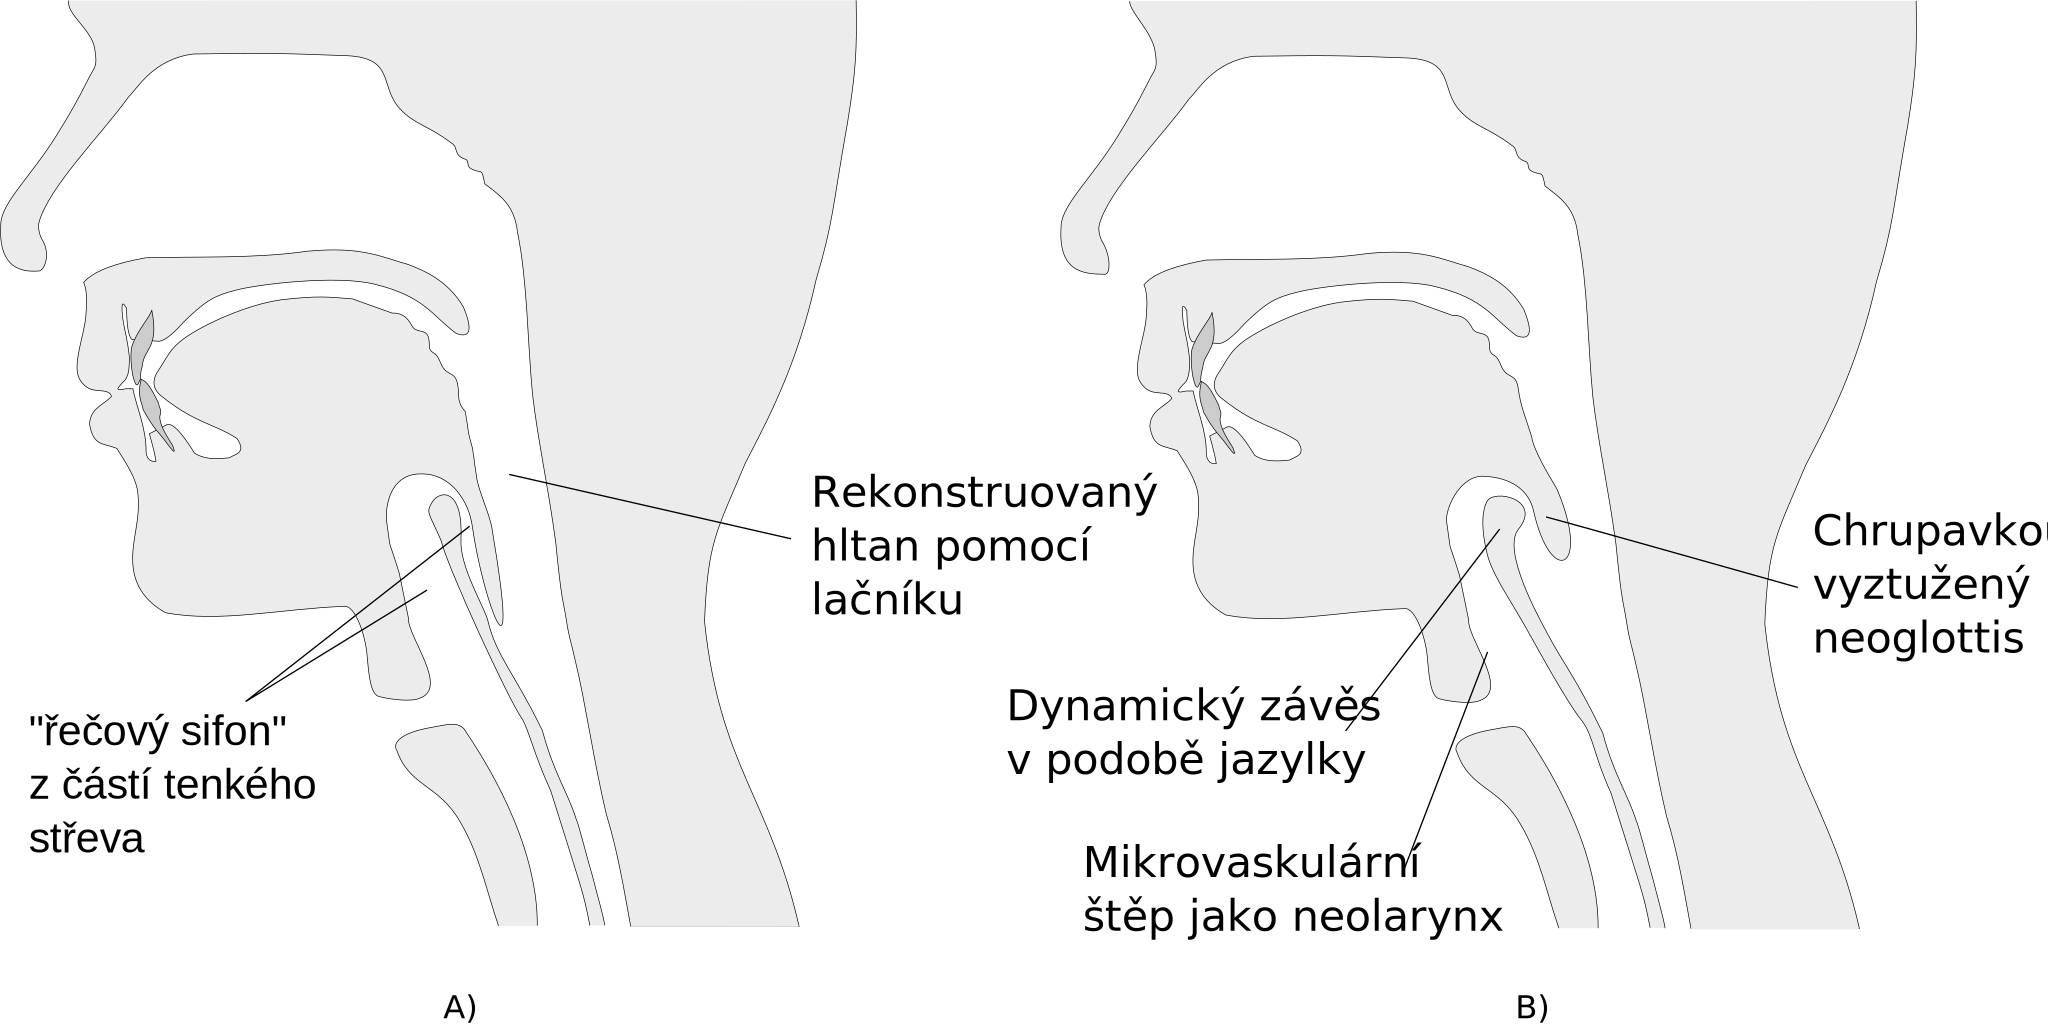
\includegraphics[width=0.9\linewidth]{ch2-cause/figures/microvascular}
    \caption[Schéma \uv{řečového sifónu} a laryngoplastiky]{A) Schéma \uv{řečového sifónu} tak jak jej představil Ehrenberg. B) Laryngoplastika podle Hagena}
    \label{fig:cause:treatment:microvascular}
  \end{center}
\end{figure}

Bohužel v současné době tyto metody nenacházejí širší uplatnění. Především je
to způsobeno chirurgickou náročností samotných metod, kvůli které se velmi
těžko prosazují na dalších pracovištích. Dalším aspektem, který limituje tyto
metody, je vliv na samotného pacienta. Metody předpokládají další chirurgický
zákrok vykonaný po totální laryngektomii. Tento zákrok představuje další zátěž
pro pacienta nemluvě o~možných komplikacích. I přes nedostatky těchto metod je
pochopitelná snaha lékařů o intenzivní výzkum v této oblasti. Při úspěšné
léčbě je pacient schopen produkovat hlas velmi dobré kvality a ve většině
případů nepotřebuje žádnou péči ze strany lékařů ORL.

% subsection hrtanu_podobné_struktury (end)

\subsection{Transplantace hrtanu} % (fold)
\label{sub:cause:treatment:transplantation}

Nejkomplexnější možnost rehabilitace hlasu představuje transplantace hrtanu.
V~tomto případě pacient obdrží implantovaný hrtan od dárce. Pokud je
transplantace úspěšná, přebírá transplantovaný orgán plně funkci původního
orgánu a velmi významně zvyšuje šance pacienta na plné zotavení bez trvalých
následků.

První informace spojené s výzkumem možností provedení transplantace hrtanu se
objevují již v 60. letech 20. století\footnote{Vůbec první úspěšná transplantace
orgánu (ledvin) se uskutečnila v roce 1954.}. Přesto byla první totální
hrtanová transplantace provedena až profesorem Marshallem Stromem v roce 1998
\cite{Narula2011} a do dnešních dnů byly provedeny pouze 2 kompletní
transplantace.

Prvním pacientem, který podstoupil transplantaci, byl čtyřicetiletý muž z USA.
K~laryngektomii v jeho případě vedla motocyklová nehoda, při které si pacient
rozdrtil hrtan. K incidentu došlo 20 let před transplantací. Před zákrokem
používal k~produkci řeči elektrolarynx. Dárcem orgánu byl taktéž čtyřicetiletý
muž, který zemřel na mozkové aneurysma. Úspěch transplantace se na příjemci
projevil již třetí den po operaci, kdy poprvé po 20 letech promluvil (vyslovil
anglické slovo \uv{hello}). Přibližně po 36 měsících od transplantace byl
produkovaný hlas srovnatelný s hlasem zdravého člověka. Podle vlastních slov
pacienta se po operaci jeho kvalita života \uv{nesmírně} zlepšila.
\cite{Strome2001} Doposud poslední úspěšně vykonaná transplantace byla
zaznamenána v~říjnu 2010.

Mezi hlavní důvody takto malého počtu zákroků patří množství pacientů vhodných
pro tuto proceduru. Jelikož se jedná o transplantaci dárcovského orgánu je
nutné použití imunosupresiv, tedy medikamentů zabraňující odmítnutí orgánu.
Imunosupresiva jsou však v současné době nepoužitelná u lidí trpících
rakovinou hrtanu z důvodu velmi vysokého rizika rozšíření rakoviny
\cite{Narula2011}. Další problém představuje náročnost samotného zákroku.
Předně je potřeba provést reinervaci a obnovení krevního oběhu v implantovaném
orgánu. U první provedené transplantace se nepodařilo dosáhnout kompletní
reinervace. Výsledkem tak byl velmi kvalitní generovaný hlas, ale zároveň
nebylo možné pomocí hrtanu zabezpečit bezproblémové dýchání a bylo proto nutné
ponechat tracheostomii.

Poslední výzkum v oblasti imunosuprese však naznačuje, že by v dohledné době
mohlo dojít k pokroku a umožnit transplantaci hrtanu i u lidí trpících
rozsáhlou rakovinou v oblasti krku \cite{Narula2011}. Prozatím je však tato
metoda vhodná pro pacienty netrpící rakovinou, případně ty, u kterých
převažovaly benigní nádory a již 5 let nedošlo k recidivě.

% subsection transplantace_hrtanu (end)

\subsection{Shrnutí} % (fold) \label{sub:treatment:summary}

% NOTE: Neni lepsi pouzit dusledky misto nasledky 3

Rehabilitaci pacientů, kteří prodělali chirurgické odstranění hrtanu, je ve
vyspělých zemích věnována značná pozornost, jelikož následky této operace,
oproti jiným druhům léčby, velmi významně ovlivňují kvalitu života pacientů. V
první řadě se léčený musí vyrovnat se ztrátou hlasu. Tato situace je již sama
o sobě velmi náročnou psychickou zkouškou. Ztráta hlasu je však pouze jedním z
vícero problémů, se kterými je potřeba se vypořádat. Mezi další patří možná
ztráta čichu či vyšší náchylnost k respiračním onemocněním. Neméně významnou
roli sehrává i fyzická odlišnost a z~toho pramenící psychická zátěž pacienta
po absolvované léčbě.

 V současnosti
nejpoužívanějšími metodami rehabilitace hlasu jsou \textbf{tracheoezofageální
píštěl} (popsáno v části \ref{sub:cause:treatment:tracheo}), \textbf{jícnový
hlas} (\ref{ssub:cause:treatment:foniatric:esophageal}) a použití
\textbf{elektrolarynxu} (\ref{ssub:cause:treatment:foniatric:elektrolarynx}).
Existují samozřejmě i další a přehled v současnosti používaných je uveden
v~tab. \ref{tab:treatment:summary}.

\newcolumntype{b}{X}
\newcolumntype{s}{>{\hsize=.5\hsize}X}

\begin{table}[ht]
  \centering
  \begin{tabularx}{1.0\textwidth}{L{1.2} L{0.6} L{1.1} L{1.1}}
    & \textbf{Kvalita} & \textbf{Výhody} & \textbf{Nevýhody} \\
    \toprule \\ [-1.75ex]

    \textbf{Tracheoezofageální píštěl} & Vysoká & Vysoká míra osvojení, dlouhá fonační doba & Zanášení píštěle a s ním spojené čištění, případně dodatečná lékařská péče \\
    \midrule \\ [-1.75ex]

    \textbf{Jícnový hlas} & Dobrá & Volné ruce při mluvení, není potřeba dodatečné lékařské péče & Velmi náročná metoda k naučení, nepřirozený hlas \\
    \midrule \\ [-1.75ex]

    \textbf{Elektrolarynx} & Nízká & Snadné k naučení & Monotonní až robotický hlas, nutné nosit externí elektrické zařízení \\
    \midrule \\ [-1.75ex]

    \textbf{Hrtanu podobné struktury} & Vysoká & Nezávislost pacienta na pravidelné lékařské péči & Velmi náročná chirurgická procedura, která pacienta vystavuje dalším možným rizikům  \\
    \midrule \\ [-1.75ex]

    \textbf{Transplantace hrtanu} & Velmi vysoká & Transplantovaný hrtan přejímá funkci odstraněného orgánu & Velmi náročná chirurgická procedura, která je vhodná jen pro malé procento pacientů \\
  \end{tabularx}

  \caption{Přehled dostupných metod rehabilitace hlasu \label{tab:treatment:summary}}
\end{table}

Většina pacientů je tedy rehabilitována pomocí tracheoezofageálního píštěle,
který principiálně vychází z jícnového hlasu, jehož negativa se snaží
eliminovat. O úspěchu rehabilitace, stejně jako u jícnového hlasu, tak
především rozhodují vlastnosti faryngoezofageálního segmentu. Pokud pacient
není schopen si osvojit jícnový hlas, případně nemá voperován píštěl, je
použit elektrolarynx. Bohužel tyto metody neřeší další problémy spojené s
odstraněním hrtanu, a proto se lékaři stále snaží zdokonalovat rehabilitační
metody. Za nejkomplexnější se dá považovat úplná transplantace hrtanu, která
řeší víceméně všechny problémy spojené s odstraněním hrtanu. Bohužel tento
zákrok je velmi náročný a vhodný pouze pro malou část pacientů.
I když je tedy v současné době lékařská věda schopna rehabilitovat hlas, tak
zde zůstává otevřený prostor pro inovace a tím zlepšení kvality života lidí
postižených ztrátou hrtanu.

% subsection treatment:summary (end)

% section rehabilitace_hlasu_po_totalni_laryngektomii (end)

% %!TEX root = ../thesis.tex
\section{Příčiny ztráty hlasu}
\label{chap:cause:desease}

Nejčastěji je trvalá ztráta hlasu zapříčiněna chirurgickým zákrokem zvaným
totální laryngektomie\footnote{\textbf{laryngektomie}: larynx, laryngos -
hrtan, ectos, ectomia - odstranění, vynětí} neboli úplné odstranění hrtanu.
Odstraněním hrtanu, a tím i hlasivek (glottis), přichází člověk o~schopnost
rozvibrovat vzduch vycházející z~plic, který je dále modulován artikulačním
ústrojím. Nejběžnější příčinou vedoucí k totální laryngektomii představuje
rakovina hrtanu v~pokročilém stádiu. V~mnohem nižší míře je na vině rakovina
hltanu či poškození hrtanu automobilovou nebo jinou traumatickou nehodou.
Podle \cite{Slavicek2000} přibude v České republice ročně přibližně 400 nových
onemocnění rakoviny hrtanu, z toho je přibližně jedna třetina léčena pomocí
totální laryngektomie. To představuje více než 100 nových případů trvalé
ztráty hlasu každý rok.

\subsection{Rakovina hrtanu} % (fold)
\label{chap:cause:desease:cancer}

Jak již bylo zmíněno, rakovina hrtanu je jedním z hlavních důvodů odstranění
hrtanu. Tento typ rakoviny postihuje převážně muže ve věku 50-60 let.
V~posledních letech je však zřejmý trend snižujícího se průměrného věku
pacientů \cite{Skvrnakova2010}. Z~celkovém počtu pacientů zhruba 20\%
představují ženy.

Přesná příčina vzniku nádorovitého onemocnění hrtanu doposud není známa, ale
z~průzkumů je zřejmá korelace mezi vznikem rakoviny a konzumací alkoholu či
kouřením. Jinými slovy, mezi rizikovou skupinu patří lidé, kteří jsou
pravidelně vystavováni vlivu kouření, ať již aktivně (sami kouří) či pasivně
(vdechují cigaretový kouř) a zároveň si dopřávají nemalé množství alkoholu.
Podle \cite{Skvrnakova2010} 90\% pacientů aktivně kuří.

\subsubsection{Příznaky onemocněni} % (fold)
\label{chap:cause:desease:cancer:symptom}

Vznikající nádorové onemocnění v oblasti hrtanu se může projevovat různými
způsoby. Mezi hlavní faktory ovlivňující počáteční příznaky patří umístění a
velikost nádoru.

Již ve velmi raném stádiu, kdy je nádor umístěn přímo na hlasivkách, je
příznakem \textbf{chrapot}. Ve většině případů se samozřejmě jedná o
krátkodobé postižení hlasivek virovou infekcí. Nicméně pokud chrapot trvá déle
než tři týdny, je již doporučováno navštívit odborného lékaře.
U nádorů nacházejících se ve vchodu do hrtanu a v polykacích cestách se mohou
jako příznak objevovat \textbf{polykací obtíže}. Mezi další možné příznaky
patří \textbf{bolesti v~krku}, jednostranné bolesti vystřelující do ucha čí
nepříjemný pocit při polykání. I~v~tomto případě krátkodobý výskyt nemusí
nutně znamenat rakovinu hrtanu, nicméně při obtížích trvajících déle než měsíc
je doporučováno důkladné  vyšetření lékařem.
Na základě umístění nádoru se může objevovat \textbf{dráždivý kašel} s možným
vykašláváním krve. Dalším možným příznakem je vznik \textbf{zduření na krku}.
V tomto případě je vhodné neprodleně vyhledat lékaře.

Z výše uvedených příznaků je zřejmé, že prvotní indicie o vážném onemocnění
mohou být podceněny, a tím značně snížena šance na plné uzdravení pacienta.
V~případě včasného diagnostikování rakoviny hrtanu či hltanu je možnost
úplného vyléčení pacienta bez trvalých následků více než 90\%
\cite{Slavicek2000}.

% subsubsection příznaky_onemocnění (end)

\subsubsection{Léčba nádorového onemocnění} % (fold)
\label{chap:cause:desease:cancer:treatment}

U nádorovitých onemocnění se v drtivé většině případů využívá
\textbf{chirurgické léčby}, \textbf{aktinoterapie} neboli ozařování a
\textbf{chemoterapie}. Nejinak tomu je i v případě rakoviny hrtanu a
polykacích cest obecně. Majoritní část pacientů je zpravidla nejprve
konfrontována s chirurgickou léčbou. Mezi nejčastější zákroky patří
\textbf{tracheostomie}, parciální laryngektomie, \textbf{totální
laryngektomie} a chordektomie. V~rámci této práce budou blíže popsány pouze
léčebné postupy přímo související s úplným odstraněním hrtanu a hlasivek.

Totální laryngektomie (TL), jak už název napovídá, představuje chirurgický
zákrok, při kterém je úplně odstraněn hrtan. V určitých případech může být
odstraněna i menší či větší část hltanu. Tento zákrok, ve spojení s léčbou
rakoviny hrtanu, poprvé vykonal Dr. Theodor Billroth 31. prosince roku 1873 ve
Vídni \cite{Gussenbauer1874} a do dnešní doby přežil v podstatě nezměněn.
Cílem této operace je odstranění orgánu zasaženého rakovinným bujením, a tedy
zamezení dalšího šíření nemoci. Součástí hrtanu je také hrtanová příklopka
(latinsky epiglottis), která zamezuje vdechnutí potravy nebo tekutin do
dýchacích cest. Po odstranění hrtanu by tedy potrava a tekutiny mohly být
vdechnuty do plic a z tohoto důvodu jsou jícen a průdušnice trvale odděleny.
Rozdíl mezi zdravým člověkem a osobou po totální laryngektomii je znázorněn na
obr. \ref{fig:cause:desease:laryngectomy}.

\begin{figure}[htb]
  \begin{center}
    \def\svgwidth{0.9\linewidth}
    % %LaTeX with PSTricks extensions
%%Creator: 0.48.3.1
%%Please note this file requires PSTricks extensions
\psset{xunit=.5pt,yunit=.5pt,runit=.5pt}
\begin{pspicture}(2907.24389648,1381.22814941)
{
\newrgbcolor{curcolor}{0.9254902 0.9254902 0.9254902}
\pscustom[linestyle=none,fillstyle=solid,fillcolor=curcolor]
{
\newpath
\moveto(70.56024,976.91215941)
\curveto(75.70194,998.05546941)(75.05233,1002.21845941)(63.72468,1022.97718941)
\curveto(59.11246,1029.25078941)(55.53152,1042.76249941)(57.82397,1051.05492941)
\curveto(72.33535,1103.54679941)(151.12483,1181.98458841)(191.6593,1238.29379441)
\curveto(203.82655,1249.22791741)(227.588336,1294.48932741)(288.348581,1301.70009441)
\curveto(395.40091,1303.19005241)(412.940729,1303.02200041)(510.35569,1299.36034741)
\curveto(591.16393,1298.04450341)(563.1446,1253.97868341)(596.12059,1219.46677821)
\curveto(617.11351,1196.64470041)(637.32731,1195.59050941)(673.24323,1168.28753341)
\curveto(683.09539,1161.70729041)(674.18628,1150.76886041)(694.17272,1144.46094641)
\curveto(700.8548,1138.26728041)(689.58524,1131.75588441)(714.56462,1126.38918541)
\curveto(718.47149,1127.09967441)(720.01648,1117.64831941)(721.82813,1108.38187941)
\curveto(742.89519,1091.67695941)(766.01459,1078.47903941)(770.6489,1036.21205941)
\curveto(785.52916,964.13363941)(785.41095,874.88456941)(793.05455,794.70262941)
\curveto(801.16608,725.36812941)(797.04543,665.20049941)(808.62059,580.55167941)
\curveto(817.99398,520.80324941)(824.99343,461.05482941)(838.33757,401.30639941)
\curveto(852.58351,343.43859941)(884.634,245.85682941)(902.96021,169.23090941)
\curveto(920.58527,111.57990941)(928.99355,58.22450941)(939.28097,2.24980941)
\lineto(1191.38979,0.50000941)
\curveto(1147.46289,192.92300941)(1072.39851,239.15118941)(1049.32187,456.03356941)
\curveto(1054.33227,575.87003941)(1066.33852,587.71091941)(1110.16719,692.25659941)
\curveto(1142.86475,756.08452941)(1187.16897,836.01858941)(1215.75173,966.06054941)
\curveto(1241.69732,1053.47858941)(1239.12891,1068.56755941)(1262.28051,1198.70444641)
\curveto(1274.15414,1272.24631941)(1276.84845,1302.56969941)(1275.20381,1380.20462941)
\curveto(1243.6598,1381.01350941)(132.01823,1379.13434941)(108.97269,1379.62040941)
\curveto(89.62734,1380.02842941)(136.091,1338.49754941)(140.67855,1310.22027841)
\curveto(145.31215,1281.65916741)(141.36641,1284.78090841)(130.36263,1262.73876141)
\curveto(114.38301,1230.72928461)(103.72405,1212.44353221)(84.57988,1181.51309641)
\curveto(46.3326,1119.71856941)(3.13314,1081.66825941)(0.88674,1049.70937941)
\curveto(-3.93696,981.08423941)(37.32565,977.54602941)(70.95213,976.84547941)
}
}
{
\newrgbcolor{curcolor}{0 0 0}
\pscustom[linewidth=1,linecolor=curcolor]
{
\newpath
\moveto(70.56024,976.91215941)
\curveto(75.70194,998.05546941)(75.05233,1002.21845941)(63.72468,1022.97718941)
\curveto(59.11246,1029.25078941)(55.53152,1042.76249941)(57.82397,1051.05492941)
\curveto(72.33535,1103.54679941)(151.12483,1181.98458841)(191.6593,1238.29379441)
\curveto(203.82655,1249.22791741)(227.588336,1294.48932741)(288.348581,1301.70009441)
\curveto(395.40091,1303.19005241)(412.940729,1303.02200041)(510.35569,1299.36034741)
\curveto(591.16393,1298.04450341)(563.1446,1253.97868341)(596.12059,1219.46677821)
\curveto(617.11351,1196.64470041)(637.32731,1195.59050941)(673.24323,1168.28753341)
\curveto(683.09539,1161.70729041)(674.18628,1150.76886041)(694.17272,1144.46094641)
\curveto(700.8548,1138.26728041)(689.58524,1131.75588441)(714.56462,1126.38918541)
\curveto(718.47149,1127.09967441)(720.01648,1117.64831941)(721.82813,1108.38187941)
\curveto(742.89519,1091.67695941)(766.01459,1078.47903941)(770.6489,1036.21205941)
\curveto(785.52916,964.13363941)(785.41095,874.88456941)(793.05455,794.70262941)
\curveto(801.16608,725.36812941)(797.04543,665.20049941)(808.62059,580.55167941)
\curveto(817.99398,520.80324941)(824.99343,461.05482941)(838.33757,401.30639941)
\curveto(852.58351,343.43859941)(884.634,245.85682941)(902.96021,169.23090941)
\curveto(920.58527,111.57990941)(928.99355,58.22450941)(939.28097,2.24980941)
\lineto(1191.38979,0.50000941)
\curveto(1147.46289,192.92300941)(1072.39851,239.15118941)(1049.32187,456.03356941)
\curveto(1054.33227,575.87003941)(1066.33852,587.71091941)(1110.16719,692.25659941)
\curveto(1142.86475,756.08452941)(1187.16897,836.01858941)(1215.75173,966.06054941)
\curveto(1241.69732,1053.47858941)(1239.12891,1068.56755941)(1262.28051,1198.70444641)
\curveto(1274.15414,1272.24631941)(1276.84845,1302.56969941)(1275.20381,1380.20462941)
\curveto(1243.6598,1381.01350941)(132.01823,1379.13434941)(108.97269,1379.62040941)
\curveto(89.62734,1380.02842941)(136.091,1338.49754941)(140.67855,1310.22027841)
\curveto(145.31215,1281.65916741)(141.36641,1284.78090841)(130.36263,1262.73876141)
\curveto(114.38301,1230.72928461)(103.72405,1212.44353221)(84.57988,1181.51309641)
\curveto(46.3326,1119.71856941)(3.13314,1081.66825941)(0.88674,1049.70937941)
\curveto(-3.93696,981.08423941)(37.32565,977.54602941)(70.95213,976.84547941)
}
}
{
\newrgbcolor{curcolor}{0.9254902 0.9254902 0.9254902}
\pscustom[linestyle=none,fillstyle=solid,fillcolor=curcolor]
{
\newpath
\moveto(663.80927,347.06111941)
\curveto(631.30672,407.78342941)(641.93353,444.78459941)(659.09229,478.19318941)
\curveto(742.49859,629.54060941)(751.64804,687.40579941)(724.24075,702.51595941)
\curveto(719.95848,704.09435941)(719.37506,696.51114941)(718.82765,695.21471941)
\curveto(711.30272,677.39364941)(710.58153,663.97482941)(687.1752,642.50022941)
\curveto(674.22342,633.07831941)(649.93085,632.99143941)(659.17482,660.02528941)
\curveto(668.2034,687.86169941)(679.75486,701.25992941)(690.49227,721.54170941)
\curveto(694.32384,735.78587941)(706.54118,754.42062941)(692.9595,768.66479941)
\curveto(680.15631,783.42381941)(684.07081,790.42534941)(682.11354,805.65799941)
\curveto(679.75193,823.26346941)(674.12318,822.66506941)(666.00743,828.02760941)
\curveto(655.05672,835.06925941)(656.16371,849.42328941)(646.73777,855.61704941)
\curveto(638.64629,860.32035941)(639.52383,863.34606941)(639.1639,872.76681941)
\curveto(637.98441,879.54741941)(638.28659,886.96301941)(625.74214,888.87292941)
\curveto(612.81159,891.73856941)(614.30292,897.00785941)(610.53081,901.39990941)
\curveto(604.8368,911.05283941)(596.12842,916.18422941)(583.68728,915.71645941)
\lineto(524.93857,936.77567941)
\curveto(490.25612,939.54036941)(474.30758,942.06391941)(418.15221,935.40170941)
\curveto(366.534745,928.00029941)(304.2199481,899.10557941)(274.750996,878.48752941)
\curveto(252.003981,862.15967941)(248.537062,849.31921941)(235.769747,830.34131941)
\curveto(222.937923,811.90137941)(230.373646,798.51614941)(242.774499,789.96747941)
\curveto(292.076635,750.86082941)(319.3103455,750.81408941)(352.832959,728.70655941)
\curveto(367.325625,706.91548941)(350.454946,706.03330941)(341.200769,700.07346941)
\curveto(321.2014438,697.73427941)(302.607692,697.85483941)(289.303279,707.23173941)
\curveto(270.762837,737.31808941)(256.564999,752.92908941)(248.143209,749.28659941)
\lineto(222.194469,735.86482941)
\curveto(228.231101,714.79611941)(231.053383,702.29899941)(232.037089,694.70475941)
\curveto(221.981864,693.29911941)(217.293619,701.68940941)(217.241359,710.28672941)
\curveto(217.477079,744.22373941)(203.2615,775.02108941)(197.55611,802.97364941)
\lineto(187.29789,802.97364941)
\curveto(166.56822,797.91572941)(178.05638,806.67132941)(182.82396,812.81626941)
\curveto(193.34887,820.71151941)(191.8352,839.37924941)(192.55804,848.77977941)
\curveto(189.01508,880.83561941)(186.10484,884.60710941)(182.56189,907.38269941)
\curveto(180.76794,924.17114941)(180.01497,937.66317941)(188.19267,922.87472941)
\curveto(188.49625,897.84202941)(190.8841,881.14644941)(196.24573,876.34594941)
\lineto(237.405799,873.66159941)
\curveto(248.143914,876.10038941)(260.863359,888.38046941)(274.091949,903.18947941)
\curveto(307.5567096,935.85866941)(321.1413212,942.22030941)(351.196907,949.82680941)
\curveto(383.523382,958.67919941)(501.87189,972.81484941)(557.73854,958.66609941)
\curveto(632.46539,940.77852941)(644.32636,910.80136941)(679.42919,885.29378941)
\curveto(701.57916,877.19347941)(703.43081,892.29125941)(690.1666,924.66429941)
\curveto(667.08021,963.46625941)(633.47421,978.37656941)(608.19846,987.93189941)
\curveto(565.49811,999.98699941)(539.14436,1015.15373941)(457.78478,1007.87922941)
\curveto(379.904483,996.64752941)(297.741184,1000.16294941)(216.825769,998.03659941)
\curveto(173.57623,990.17701941)(140.18925,979.41667941)(124.29082,961.33378941)
\curveto(130.726,946.56084941)(128.46979,924.48665941)(127.58388,911.82347941)
\curveto(125.77419,885.95569941)(110.07974,846.59298941)(115.57181,824.08208941)
\curveto(117.8965,814.55367941)(126.13355,805.09264941)(135.50065,802.07764941)
\curveto(146.31169,798.59789941)(163.07609,802.37811941)(165.7171,791.42292941)
\curveto(153.73391,778.74919941)(133.98029,773.84590941)(133.09836,750.07091941)
\curveto(138.68162,717.00597941)(153.29258,722.31734941)(173.72208,714.04142941)
\curveto(187.02623,693.18217941)(200.39377,672.31353941)(204.32814,652.84226941)
\curveto(210.9065,607.17595941)(194.37244,578.73022941)(197.73702,539.26597941)
\curveto(200.49791,508.68349941)(217.093467,485.47951941)(246.536796,469.12768941)
\curveto(327.687696,453.96820941)(416.73819,474.96141941)(510.92789,478.67598941)
\curveto(530.04251,482.78327941)(545.67914,429.27048941)(546.81162,402.15754941)
\curveto(549.12588,378.19912941)(560.21646,359.01453941)(567.26823,339.79363941)
\curveto(599.04903,283.26154941)(653.26269,213.99460941)(685.53957,157.14470941)
\curveto(714.54359,107.81710941)(724.30311,55.08410941)(742.45504,2.65910941)
\curveto(791.06479,2.93720941)(798.38877,2.65910941)(798.38877,2.65910941)
\curveto(799.22188,128.23700941)(690.30166,284.55155941)(663.80927,347.06111941)
\closepath
}
}
{
\newrgbcolor{curcolor}{0 0 0}
\pscustom[linewidth=1,linecolor=curcolor]
{
\newpath
\moveto(663.80927,347.06111941)
\curveto(631.30672,407.78342941)(641.93353,444.78459941)(659.09229,478.19318941)
\curveto(742.49859,629.54060941)(751.64804,687.40579941)(724.24075,702.51595941)
\curveto(719.95848,704.09435941)(719.37506,696.51114941)(718.82765,695.21471941)
\curveto(711.30272,677.39364941)(710.58153,663.97482941)(687.1752,642.50022941)
\curveto(674.22342,633.07831941)(649.93085,632.99143941)(659.17482,660.02528941)
\curveto(668.2034,687.86169941)(679.75486,701.25992941)(690.49227,721.54170941)
\curveto(694.32384,735.78587941)(706.54118,754.42062941)(692.9595,768.66479941)
\curveto(680.15631,783.42381941)(684.07081,790.42534941)(682.11354,805.65799941)
\curveto(679.75193,823.26346941)(674.12318,822.66506941)(666.00743,828.02760941)
\curveto(655.05672,835.06925941)(656.16371,849.42328941)(646.73777,855.61704941)
\curveto(638.64629,860.32035941)(639.52383,863.34606941)(639.1639,872.76681941)
\curveto(637.98441,879.54741941)(638.28659,886.96301941)(625.74214,888.87292941)
\curveto(612.81159,891.73856941)(614.30292,897.00785941)(610.53081,901.39990941)
\curveto(604.8368,911.05283941)(596.12842,916.18422941)(583.68728,915.71645941)
\lineto(524.93857,936.77567941)
\curveto(490.25612,939.54036941)(474.30758,942.06391941)(418.15221,935.40170941)
\curveto(366.534745,928.00029941)(304.2199481,899.10557941)(274.750996,878.48752941)
\curveto(252.003981,862.15967941)(248.537062,849.31921941)(235.769747,830.34131941)
\curveto(222.937923,811.90137941)(230.373646,798.51614941)(242.774499,789.96747941)
\curveto(292.076635,750.86082941)(319.3103455,750.81408941)(352.832959,728.70655941)
\curveto(367.325625,706.91548941)(350.454946,706.03330941)(341.200769,700.07346941)
\curveto(321.2014438,697.73427941)(302.607692,697.85483941)(289.303279,707.23173941)
\curveto(270.762837,737.31808941)(256.564999,752.92908941)(248.143209,749.28659941)
\lineto(222.194469,735.86482941)
\curveto(228.231101,714.79611941)(231.053383,702.29899941)(232.037089,694.70475941)
\curveto(221.981864,693.29911941)(217.293619,701.68940941)(217.241359,710.28672941)
\curveto(217.477079,744.22373941)(203.2615,775.02108941)(197.55611,802.97364941)
\lineto(187.29789,802.97364941)
\curveto(166.56822,797.91572941)(178.05638,806.67132941)(182.82396,812.81626941)
\curveto(193.34887,820.71151941)(191.8352,839.37924941)(192.55804,848.77977941)
\curveto(189.01508,880.83561941)(186.10484,884.60710941)(182.56189,907.38269941)
\curveto(180.76794,924.17114941)(180.01497,937.66317941)(188.19267,922.87472941)
\curveto(188.49625,897.84202941)(190.8841,881.14644941)(196.24573,876.34594941)
\lineto(237.405799,873.66159941)
\curveto(248.143914,876.10038941)(260.863359,888.38046941)(274.091949,903.18947941)
\curveto(307.5567096,935.85866941)(321.1413212,942.22030941)(351.196907,949.82680941)
\curveto(383.523382,958.67919941)(501.87189,972.81484941)(557.73854,958.66609941)
\curveto(632.46539,940.77852941)(644.32636,910.80136941)(679.42919,885.29378941)
\curveto(701.57916,877.19347941)(703.43081,892.29125941)(690.1666,924.66429941)
\curveto(667.08021,963.46625941)(633.47421,978.37656941)(608.19846,987.93189941)
\curveto(565.49811,999.98699941)(539.14436,1015.15373941)(457.78478,1007.87922941)
\curveto(379.904483,996.64752941)(297.741184,1000.16294941)(216.825769,998.03659941)
\curveto(173.57623,990.17701941)(140.18925,979.41667941)(124.29082,961.33378941)
\curveto(130.726,946.56084941)(128.46979,924.48665941)(127.58388,911.82347941)
\curveto(125.77419,885.95569941)(110.07974,846.59298941)(115.57181,824.08208941)
\curveto(117.8965,814.55367941)(126.13355,805.09264941)(135.50065,802.07764941)
\curveto(146.31169,798.59789941)(163.07609,802.37811941)(165.7171,791.42292941)
\curveto(153.73391,778.74919941)(133.98029,773.84590941)(133.09836,750.07091941)
\curveto(138.68162,717.00597941)(153.29258,722.31734941)(173.72208,714.04142941)
\curveto(187.02623,693.18217941)(200.39377,672.31353941)(204.32814,652.84226941)
\curveto(210.9065,607.17595941)(194.37244,578.73022941)(197.73702,539.26597941)
\curveto(200.49791,508.68349941)(217.093467,485.47951941)(246.536796,469.12768941)
\curveto(327.687696,453.96820941)(416.73819,474.96141941)(510.92789,478.67598941)
\curveto(530.04251,482.78327941)(545.67914,429.27048941)(546.81162,402.15754941)
\curveto(549.12588,378.19912941)(560.21646,359.01453941)(567.26823,339.79363941)
\curveto(599.04903,283.26154941)(653.26269,213.99460941)(685.53957,157.14470941)
\curveto(714.54359,107.81710941)(724.30311,55.08410941)(742.45504,2.65910941)
\curveto(791.06479,2.93720941)(798.38877,2.65910941)(798.38877,2.65910941)
\curveto(799.22188,128.23700941)(690.30166,284.55155941)(663.80927,347.06111941)
\closepath
}
}
{
\newrgbcolor{curcolor}{0.9254902 0.9254902 0.9254902}
\pscustom[linestyle=none,fillstyle=solid,fillcolor=curcolor]
{
\newpath
\moveto(895.41899,4.16750941)
\curveto(885.42628,56.53280941)(902.19573,58.71910941)(839.94237,209.07310941)
\curveto(814.28299,265.00824941)(789.33265,331.01818941)(787.1501,353.13337941)
\curveto(783.27094,384.03743941)(774.61723,398.97336941)(768.35964,416.66306941)
\curveto(765.06171,427.11926941)(764.824,429.14654941)(763.88572,437.24309941)
\curveto(772.18552,469.13804941)(790.10614,446.64287941)(796.99273,433.66395941)
\curveto(806.54018,410.67444941)(809.23317,396.02182941)(815.7832,375.50298941)
\curveto(825.27074,319.54128941)(827.96413,320.89590941)(833.67888,296.76197941)
\curveto(850.02247,234.61056941)(859.17548,212.00730941)(871.25982,173.28180941)
\curveto(877.50757,164.14560941)(890.91697,125.77240941)(901.68248,69.48680941)
\curveto(911.70975,10.97790941)(908.84075,23.55460941)(912.41989,3.27280941)
\closepath
}
}
{
\newrgbcolor{curcolor}{0 0 0}
\pscustom[linewidth=1,linecolor=curcolor]
{
\newpath
\moveto(895.41899,4.16750941)
\curveto(885.42628,56.53280941)(902.19573,58.71910941)(839.94237,209.07310941)
\curveto(814.28299,265.00824941)(789.33265,331.01818941)(787.1501,353.13337941)
\curveto(783.27094,384.03743941)(774.61723,398.97336941)(768.35964,416.66306941)
\curveto(765.06171,427.11926941)(764.824,429.14654941)(763.88572,437.24309941)
\curveto(772.18552,469.13804941)(790.10614,446.64287941)(796.99273,433.66395941)
\curveto(806.54018,410.67444941)(809.23317,396.02182941)(815.7832,375.50298941)
\curveto(825.27074,319.54128941)(827.96413,320.89590941)(833.67888,296.76197941)
\curveto(850.02247,234.61056941)(859.17548,212.00730941)(871.25982,173.28180941)
\curveto(877.50757,164.14560941)(890.91697,125.77240941)(901.68248,69.48680941)
\curveto(911.70975,10.97790941)(908.84075,23.55460941)(912.41989,3.27280941)
\closepath
}
}
{
\newrgbcolor{curcolor}{0.3019608 0.3019608 0.3019608}
\pscustom[linewidth=1,linecolor=curcolor]
{
\newpath
\moveto(777.30748,456.03356941)
\curveto(752.3253,471.35452941)(763.78475,491.53873941)(758.09534,500.48890941)
\curveto(752.61989,509.10247941)(742.51461,537.74873941)(752.25352,555.80199941)
\curveto(755.72774,560.13621941)(760.22549,596.01455941)(758.06962,633.64822941)
\curveto(756.02394,662.52158941)(739.67178,681.85842941)(729.88392,700.30964941)
}
}
{
\newrgbcolor{curcolor}{0.9254902 0.9254902 0.9254902}
\pscustom[linestyle=none,fillstyle=solid,fillcolor=curcolor]
{
\newpath
\moveto(1701.66159587,977.23068781)
\curveto(1706.80329587,998.37399781)(1706.15369587,1002.53698781)(1694.82599587,1023.29571781)
\curveto(1690.21379587,1029.56931781)(1686.63289587,1043.08102781)(1688.92529587,1051.37344781)
\curveto(1703.43669587,1103.86531781)(1782.22619587,1182.30311781)(1822.76069587,1238.61232781)
\curveto(1834.92789587,1249.54644781)(1858.68969587,1294.80786081)(1919.44989587,1302.01863081)
\curveto(2026.50229587,1303.50859081)(2044.04209587,1303.34053081)(2141.45699587,1299.67888081)
\curveto(2222.26529587,1298.36304081)(2194.24599587,1254.29721781)(2227.22189587,1219.78530781)
\curveto(2248.21489587,1196.96322781)(2268.42869587,1195.90903781)(2304.34459587,1168.60606781)
\curveto(2314.19669587,1162.02581781)(2305.28759587,1151.08738781)(2325.27409587,1144.77947781)
\curveto(2331.95619587,1138.58580781)(2320.68659587,1132.07441781)(2345.66599587,1126.70771781)
\curveto(2349.57279587,1127.41820781)(2351.11779587,1117.96683781)(2352.92949587,1108.70039781)
\curveto(2373.99649587,1091.99547781)(2397.11589587,1078.79755781)(2401.75029587,1036.53058781)
\curveto(2416.63049587,964.45216781)(2416.51229587,875.20310781)(2424.15589587,795.02115781)
\curveto(2432.26739587,725.68664781)(2428.14679587,665.51901781)(2439.72189587,580.87019781)
\curveto(2449.09529587,521.12176781)(2456.09479587,461.37334781)(2469.43889587,401.62491781)
\curveto(2483.68489587,343.75712781)(2515.73539587,246.17532781)(2534.06159587,169.54942781)
\curveto(2551.68659587,111.89842781)(2560.09489587,58.54302781)(2570.38229587,2.56832781)
\lineto(2822.49109587,0.81852781)
\curveto(2778.56419587,193.24152781)(2703.49979587,239.46972781)(2680.42319587,456.35208781)
\curveto(2685.43359587,576.18855781)(2697.43979587,588.02943781)(2741.26849587,692.57511781)
\curveto(2773.96599587,756.40305781)(2818.27029587,836.33711781)(2846.85299587,966.37907781)
\curveto(2872.79859587,1053.79710781)(2870.23019587,1068.88607781)(2893.38179587,1199.02297781)
\curveto(2905.25539587,1272.56484781)(2907.94969587,1302.88823081)(2906.30509587,1380.5231509)
\curveto(2874.76109587,1381.3320309)(1763.11959587,1379.45287091)(1740.07399587,1379.9389309)
\curveto(1720.72869587,1380.3469509)(1767.19239587,1338.81607081)(1771.77989587,1310.53881081)
\curveto(1776.41349587,1281.97770081)(1772.46779587,1285.09944081)(1761.46399587,1263.05728781)
\curveto(1745.48439587,1231.04781781)(1734.82539587,1212.76205781)(1715.68119587,1181.83162781)
\curveto(1677.43399587,1120.03708781)(1634.23449587,1081.98677781)(1631.98809587,1050.02789781)
\curveto(1627.16439587,981.40276781)(1668.42699587,977.86455781)(1702.05349587,977.16400781)
}
}
{
\newrgbcolor{curcolor}{0 0 0}
\pscustom[linewidth=1,linecolor=curcolor]
{
\newpath
\moveto(1701.66159587,977.23068781)
\curveto(1706.80329587,998.37399781)(1706.15369587,1002.53698781)(1694.82599587,1023.29571781)
\curveto(1690.21379587,1029.56931781)(1686.63289587,1043.08102781)(1688.92529587,1051.37344781)
\curveto(1703.43669587,1103.86531781)(1782.22619587,1182.30311781)(1822.76069587,1238.61232781)
\curveto(1834.92789587,1249.54644781)(1858.68969587,1294.80786081)(1919.44989587,1302.01863081)
\curveto(2026.50229587,1303.50859081)(2044.04209587,1303.34053081)(2141.45699587,1299.67888081)
\curveto(2222.26529587,1298.36304081)(2194.24599587,1254.29721781)(2227.22189587,1219.78530781)
\curveto(2248.21489587,1196.96322781)(2268.42869587,1195.90903781)(2304.34459587,1168.60606781)
\curveto(2314.19669587,1162.02581781)(2305.28759587,1151.08738781)(2325.27409587,1144.77947781)
\curveto(2331.95619587,1138.58580781)(2320.68659587,1132.07441781)(2345.66599587,1126.70771781)
\curveto(2349.57279587,1127.41820781)(2351.11779587,1117.96683781)(2352.92949587,1108.70039781)
\curveto(2373.99649587,1091.99547781)(2397.11589587,1078.79755781)(2401.75029587,1036.53058781)
\curveto(2416.63049587,964.45216781)(2416.51229587,875.20310781)(2424.15589587,795.02115781)
\curveto(2432.26739587,725.68664781)(2428.14679587,665.51901781)(2439.72189587,580.87019781)
\curveto(2449.09529587,521.12176781)(2456.09479587,461.37334781)(2469.43889587,401.62491781)
\curveto(2483.68489587,343.75712781)(2515.73539587,246.17532781)(2534.06159587,169.54942781)
\curveto(2551.68659587,111.89842781)(2560.09489587,58.54302781)(2570.38229587,2.56832781)
\lineto(2822.49109587,0.81852781)
\curveto(2778.56419587,193.24152781)(2703.49979587,239.46972781)(2680.42319587,456.35208781)
\curveto(2685.43359587,576.18855781)(2697.43979587,588.02943781)(2741.26849587,692.57511781)
\curveto(2773.96599587,756.40305781)(2818.27029587,836.33711781)(2846.85299587,966.37907781)
\curveto(2872.79859587,1053.79710781)(2870.23019587,1068.88607781)(2893.38179587,1199.02297781)
\curveto(2905.25539587,1272.56484781)(2907.94969587,1302.88823081)(2906.30509587,1380.5231509)
\curveto(2874.76109587,1381.3320309)(1763.11959587,1379.45287091)(1740.07399587,1379.9389309)
\curveto(1720.72869587,1380.3469509)(1767.19239587,1338.81607081)(1771.77989587,1310.53881081)
\curveto(1776.41349587,1281.97770081)(1772.46779587,1285.09944081)(1761.46399587,1263.05728781)
\curveto(1745.48439587,1231.04781781)(1734.82539587,1212.76205781)(1715.68119587,1181.83162781)
\curveto(1677.43399587,1120.03708781)(1634.23449587,1081.98677781)(1631.98809587,1050.02789781)
\curveto(1627.16439587,981.40276781)(1668.42699587,977.86455781)(1702.05349587,977.16400781)
}
}
{
\newrgbcolor{curcolor}{0.9254902 0.9254902 0.9254902}
\pscustom[linestyle=none,fillstyle=solid,fillcolor=curcolor]
{
\newpath
\moveto(2222.18449587,263.90192781)
\curveto(2241.31109587,209.90072781)(2284.36399587,214.31312781)(2316.64089587,157.46322781)
\curveto(2345.64489587,108.13562781)(2355.40449587,55.40262781)(2373.55639587,2.97762781)
\curveto(2422.16609587,3.25572781)(2429.49009587,2.97762781)(2429.49009587,2.97762781)
\curveto(2430.32319587,128.55552781)(2351.03939587,253.41772781)(2322.64889587,295.68062781)
\curveto(2312.63549587,308.42372781)(2295.39239587,302.39362781)(2270.51859587,298.13982781)
\curveto(2228.12249587,290.36432781)(2214.62639587,275.73032781)(2222.18449587,263.90192781)
\closepath
\moveto(2241.02189587,349.02342781)
\curveto(2285.97709587,364.43132781)(2303.47489587,364.38192781)(2330.30379587,361.55452781)
\curveto(2357.48059587,352.76802781)(2383.60959587,340.11422781)(2408.12809587,311.06042781)
\curveto(2424.23029587,288.94522781)(2445.38429587,265.32672781)(2471.04369587,209.39162781)
\curveto(2533.29709587,59.03762781)(2516.52759587,56.85132781)(2526.52029587,4.48602781)
\lineto(2543.52119587,3.59132781)
\curveto(2539.94209587,23.87312781)(2542.81109587,11.29642781)(2532.78379587,69.80532781)
\curveto(2522.01829587,126.09092781)(2508.60889587,164.46412781)(2502.36119587,173.60032781)
\curveto(2490.27679587,212.32582781)(2481.12379587,234.92902781)(2464.78019587,297.08052781)
\curveto(2459.06549587,321.21442781)(2456.37209587,319.85982781)(2446.88459587,375.82152781)
\curveto(2440.33449587,396.34034781)(2416.76219587,481.22354781)(2407.21469587,504.21305781)
\curveto(2387.67399587,567.80861781)(2386.83649587,580.18045781)(2378.38959587,636.46615781)
\curveto(2376.77379587,686.52617781)(2369.04569587,693.38127781)(2355.34209587,700.93635781)
\curveto(2351.05979587,702.51475781)(2350.47639587,696.82966781)(2349.92899587,695.53323781)
\curveto(2342.40409587,677.71216781)(2341.68289587,664.29334781)(2318.27659587,642.81874781)
\curveto(2305.32479587,633.39683781)(2281.03219587,633.30995781)(2290.27619587,660.34380781)
\curveto(2299.30479587,688.18021781)(2310.85619587,701.57844781)(2321.59359587,721.86022781)
\curveto(2325.42519587,736.10439781)(2337.64249587,754.73915781)(2324.06089587,768.98332781)
\curveto(2311.25769587,783.74234781)(2315.17219587,790.74387781)(2313.21489587,805.97652781)
\curveto(2310.85329587,823.58199781)(2305.22449587,822.98359781)(2297.10879587,828.34613781)
\curveto(2286.15809587,835.38778781)(2287.26509587,849.74182781)(2277.83909587,855.93558781)
\curveto(2269.74759587,860.63889781)(2270.62519587,863.66460781)(2270.26529587,873.08535781)
\curveto(2269.08579587,879.86595781)(2269.38789587,887.28155781)(2256.84349587,889.19146781)
\curveto(2243.91289587,892.05710781)(2245.40429587,897.32639781)(2241.63219587,901.71844781)
\curveto(2235.93819587,911.37137781)(2227.22979587,916.50276781)(2214.78859587,916.03499781)
\lineto(2156.03989587,937.09421781)
\curveto(2121.35749587,939.85890781)(2105.40889587,942.38245781)(2049.25359587,935.72024781)
\curveto(1997.63609587,928.31883781)(1935.32129587,899.42411781)(1905.85229587,878.80606781)
\curveto(1883.10529587,862.47821781)(1879.63839587,849.63775781)(1866.87109587,830.65984781)
\curveto(1854.03929587,812.21990781)(1861.47499587,798.83467781)(1873.87579587,790.28600781)
\curveto(1923.17799587,751.17934781)(1950.41169587,751.13260781)(1983.93429587,729.02507781)
\curveto(1998.42699587,707.23400781)(1981.55629587,706.35182781)(1972.30209587,700.39198781)
\curveto(1952.30279587,698.05279781)(1933.70899587,698.17335781)(1920.40459587,707.55025781)
\curveto(1901.86419587,737.63660781)(1887.66629587,753.24760781)(1879.24459587,749.60511781)
\lineto(1853.29579587,736.18334781)
\curveto(1859.33249587,715.11463781)(1862.15469587,702.61751781)(1863.13839587,695.02327781)
\curveto(1853.08319587,693.61763781)(1848.39499587,702.00792781)(1848.34269587,710.60524781)
\curveto(1848.57839587,744.54225781)(1834.36289587,775.33961781)(1828.65749587,803.29217781)
\lineto(1818.39919587,803.29217781)
\curveto(1797.66959587,798.23425781)(1809.15769587,806.98985781)(1813.92529587,813.13479781)
\curveto(1824.45019587,821.03004781)(1822.93659587,839.69777781)(1823.65939587,849.09831781)
\curveto(1820.11639587,881.15415781)(1817.20619587,884.92564781)(1813.66319587,907.70123781)
\curveto(1811.86929587,924.48968781)(1811.11629587,937.98171781)(1819.29399587,923.19326781)
\curveto(1819.59759587,898.16056781)(1821.98549587,881.46498781)(1827.34709587,876.66448781)
\lineto(1868.50709587,873.98013781)
\curveto(1879.24529587,876.41892781)(1891.96469587,888.69900781)(1905.19329587,903.50801781)
\curveto(1938.65809587,936.17720781)(1952.24269587,942.53884781)(1982.29829587,950.14534781)
\curveto(2014.62469587,958.99772781)(2132.97319587,973.13337781)(2188.83989587,958.98462781)
\curveto(2263.56669587,941.09706781)(2275.42769587,911.11990781)(2310.53049587,885.61232781)
\curveto(2332.68049587,877.51201781)(2334.53219587,892.60979781)(2321.26799587,924.98283781)
\curveto(2298.18159587,963.78478781)(2264.57559587,978.69509781)(2239.29979587,988.25042781)
\curveto(2196.59949587,1000.30552781)(2170.24569587,1015.47226781)(2088.88609587,1008.19775781)
\curveto(2011.00579587,996.96605781)(1928.84249587,1000.48147781)(1847.92709587,998.35512781)
\curveto(1804.67759587,990.49554781)(1771.29059587,979.73520781)(1755.39219587,961.65231781)
\curveto(1761.82739587,946.87938781)(1759.57109587,924.80519781)(1758.68519587,912.14201781)
\curveto(1756.87549587,886.27423781)(1741.18109587,846.91151781)(1746.67319587,824.40061781)
\curveto(1748.99789587,814.87220781)(1757.23489587,805.41117781)(1766.60199587,802.39617781)
\curveto(1777.41299587,798.91642781)(1794.17739587,802.69664781)(1796.81849587,791.74145781)
\curveto(1784.83529587,779.06772781)(1765.08159587,774.16443781)(1764.19969587,750.38943781)
\curveto(1769.78299587,717.32449781)(1784.39389587,722.63586781)(1804.82339587,714.35994781)
\curveto(1818.12759587,693.50069781)(1831.49509587,672.63205781)(1835.42949587,653.16078781)
\curveto(1842.00789587,607.49447781)(1825.47379587,579.04874781)(1828.83839587,539.58449781)
\curveto(1831.59929587,509.00201781)(1848.19479587,485.79803781)(1877.63809587,469.44620781)
\curveto(1958.78899587,454.28672781)(2047.83949587,475.27993781)(2142.02919587,478.99450781)
\curveto(2161.14389587,483.10179781)(2176.78049587,429.58900781)(2177.91299587,402.47606781)
\curveto(2180.22719587,378.51762781)(2182.50489587,347.35652781)(2195.88369587,344.58602781)
\curveto(2216.40419587,339.36112781)(2230.61569587,343.95892781)(2241.02189587,349.02342781)
\closepath
}
}
{
\newrgbcolor{curcolor}{0 0 0}
\pscustom[linewidth=1,linecolor=curcolor]
{
\newpath
\moveto(2222.18449587,263.90192781)
\curveto(2241.31109587,209.90072781)(2284.36399587,214.31312781)(2316.64089587,157.46322781)
\curveto(2345.64489587,108.13562781)(2355.40449587,55.40262781)(2373.55639587,2.97762781)
\curveto(2422.16609587,3.25572781)(2429.49009587,2.97762781)(2429.49009587,2.97762781)
\curveto(2430.32319587,128.55552781)(2351.03939587,253.41772781)(2322.64889587,295.68062781)
\curveto(2312.63549587,308.42372781)(2295.39239587,302.39362781)(2270.51859587,298.13982781)
\curveto(2228.12249587,290.36432781)(2214.62639587,275.73032781)(2222.18449587,263.90192781)
\closepath
\moveto(2241.02189587,349.02342781)
\curveto(2285.97709587,364.43132781)(2303.47489587,364.38192781)(2330.30379587,361.55452781)
\curveto(2357.48059587,352.76802781)(2383.60959587,340.11422781)(2408.12809587,311.06042781)
\curveto(2424.23029587,288.94522781)(2445.38429587,265.32672781)(2471.04369587,209.39162781)
\curveto(2533.29709587,59.03762781)(2516.52759587,56.85132781)(2526.52029587,4.48602781)
\lineto(2543.52119587,3.59132781)
\curveto(2539.94209587,23.87312781)(2542.81109587,11.29642781)(2532.78379587,69.80532781)
\curveto(2522.01829587,126.09092781)(2508.60889587,164.46412781)(2502.36119587,173.60032781)
\curveto(2490.27679587,212.32582781)(2481.12379587,234.92902781)(2464.78019587,297.08052781)
\curveto(2459.06549587,321.21442781)(2456.37209587,319.85982781)(2446.88459587,375.82152781)
\curveto(2440.33449587,396.34034781)(2416.76219587,481.22354781)(2407.21469587,504.21305781)
\curveto(2387.67399587,567.80861781)(2386.83649587,580.18045781)(2378.38959587,636.46615781)
\curveto(2376.77379587,686.52617781)(2369.04569587,693.38127781)(2355.34209587,700.93635781)
\curveto(2351.05979587,702.51475781)(2350.47639587,696.82966781)(2349.92899587,695.53323781)
\curveto(2342.40409587,677.71216781)(2341.68289587,664.29334781)(2318.27659587,642.81874781)
\curveto(2305.32479587,633.39683781)(2281.03219587,633.30995781)(2290.27619587,660.34380781)
\curveto(2299.30479587,688.18021781)(2310.85619587,701.57844781)(2321.59359587,721.86022781)
\curveto(2325.42519587,736.10439781)(2337.64249587,754.73915781)(2324.06089587,768.98332781)
\curveto(2311.25769587,783.74234781)(2315.17219587,790.74387781)(2313.21489587,805.97652781)
\curveto(2310.85329587,823.58199781)(2305.22449587,822.98359781)(2297.10879587,828.34613781)
\curveto(2286.15809587,835.38778781)(2287.26509587,849.74182781)(2277.83909587,855.93558781)
\curveto(2269.74759587,860.63889781)(2270.62519587,863.66460781)(2270.26529587,873.08535781)
\curveto(2269.08579587,879.86595781)(2269.38789587,887.28155781)(2256.84349587,889.19146781)
\curveto(2243.91289587,892.05710781)(2245.40429587,897.32639781)(2241.63219587,901.71844781)
\curveto(2235.93819587,911.37137781)(2227.22979587,916.50276781)(2214.78859587,916.03499781)
\lineto(2156.03989587,937.09421781)
\curveto(2121.35749587,939.85890781)(2105.40889587,942.38245781)(2049.25359587,935.72024781)
\curveto(1997.63609587,928.31883781)(1935.32129587,899.42411781)(1905.85229587,878.80606781)
\curveto(1883.10529587,862.47821781)(1879.63839587,849.63775781)(1866.87109587,830.65984781)
\curveto(1854.03929587,812.21990781)(1861.47499587,798.83467781)(1873.87579587,790.28600781)
\curveto(1923.17799587,751.17934781)(1950.41169587,751.13260781)(1983.93429587,729.02507781)
\curveto(1998.42699587,707.23400781)(1981.55629587,706.35182781)(1972.30209587,700.39198781)
\curveto(1952.30279587,698.05279781)(1933.70899587,698.17335781)(1920.40459587,707.55025781)
\curveto(1901.86419587,737.63660781)(1887.66629587,753.24760781)(1879.24459587,749.60511781)
\lineto(1853.29579587,736.18334781)
\curveto(1859.33249587,715.11463781)(1862.15469587,702.61751781)(1863.13839587,695.02327781)
\curveto(1853.08319587,693.61763781)(1848.39499587,702.00792781)(1848.34269587,710.60524781)
\curveto(1848.57839587,744.54225781)(1834.36289587,775.33961781)(1828.65749587,803.29217781)
\lineto(1818.39919587,803.29217781)
\curveto(1797.66959587,798.23425781)(1809.15769587,806.98985781)(1813.92529587,813.13479781)
\curveto(1824.45019587,821.03004781)(1822.93659587,839.69777781)(1823.65939587,849.09831781)
\curveto(1820.11639587,881.15415781)(1817.20619587,884.92564781)(1813.66319587,907.70123781)
\curveto(1811.86929587,924.48968781)(1811.11629587,937.98171781)(1819.29399587,923.19326781)
\curveto(1819.59759587,898.16056781)(1821.98549587,881.46498781)(1827.34709587,876.66448781)
\lineto(1868.50709587,873.98013781)
\curveto(1879.24529587,876.41892781)(1891.96469587,888.69900781)(1905.19329587,903.50801781)
\curveto(1938.65809587,936.17720781)(1952.24269587,942.53884781)(1982.29829587,950.14534781)
\curveto(2014.62469587,958.99772781)(2132.97319587,973.13337781)(2188.83989587,958.98462781)
\curveto(2263.56669587,941.09706781)(2275.42769587,911.11990781)(2310.53049587,885.61232781)
\curveto(2332.68049587,877.51201781)(2334.53219587,892.60979781)(2321.26799587,924.98283781)
\curveto(2298.18159587,963.78478781)(2264.57559587,978.69509781)(2239.29979587,988.25042781)
\curveto(2196.59949587,1000.30552781)(2170.24569587,1015.47226781)(2088.88609587,1008.19775781)
\curveto(2011.00579587,996.96605781)(1928.84249587,1000.48147781)(1847.92709587,998.35512781)
\curveto(1804.67759587,990.49554781)(1771.29059587,979.73520781)(1755.39219587,961.65231781)
\curveto(1761.82739587,946.87938781)(1759.57109587,924.80519781)(1758.68519587,912.14201781)
\curveto(1756.87549587,886.27423781)(1741.18109587,846.91151781)(1746.67319587,824.40061781)
\curveto(1748.99789587,814.87220781)(1757.23489587,805.41117781)(1766.60199587,802.39617781)
\curveto(1777.41299587,798.91642781)(1794.17739587,802.69664781)(1796.81849587,791.74145781)
\curveto(1784.83529587,779.06772781)(1765.08159587,774.16443781)(1764.19969587,750.38943781)
\curveto(1769.78299587,717.32449781)(1784.39389587,722.63586781)(1804.82339587,714.35994781)
\curveto(1818.12759587,693.50069781)(1831.49509587,672.63205781)(1835.42949587,653.16078781)
\curveto(1842.00789587,607.49447781)(1825.47379587,579.04874781)(1828.83839587,539.58449781)
\curveto(1831.59929587,509.00201781)(1848.19479587,485.79803781)(1877.63809587,469.44620781)
\curveto(1958.78899587,454.28672781)(2047.83949587,475.27993781)(2142.02919587,478.99450781)
\curveto(2161.14389587,483.10179781)(2176.78049587,429.58900781)(2177.91299587,402.47606781)
\curveto(2180.22719587,378.51762781)(2182.50489587,347.35652781)(2195.88369587,344.58602781)
\curveto(2216.40419587,339.36112781)(2230.61569587,343.95892781)(2241.02189587,349.02342781)
\closepath
}
}
{
\newrgbcolor{curcolor}{0.80000001 0.80000001 0.80000001}
\pscustom[linestyle=none,fillstyle=solid,fillcolor=curcolor]
{
\newpath
\moveto(1856.91629587,920.33095781)
\curveto(1852.97789587,908.04444781)(1834.19749587,888.87896781)(1827.17899587,865.91806781)
\curveto(1825.13979587,861.15995781)(1825.04509587,833.60610781)(1830.34249587,816.56683781)
\curveto(1835.47639587,800.05400781)(1837.88419587,815.66513781)(1839.83319587,817.19954781)
\curveto(1840.15089587,828.36895781)(1841.50219587,833.33705781)(1842.99669587,837.44620781)
\curveto(1844.41779587,863.38058781)(1868.34079587,862.30071781)(1856.91629587,920.33095781)
\closepath
}
}
{
\newrgbcolor{curcolor}{0 0 0}
\pscustom[linewidth=1,linecolor=curcolor]
{
\newpath
\moveto(1856.91629587,920.33095781)
\curveto(1852.97789587,908.04444781)(1834.19749587,888.87896781)(1827.17899587,865.91806781)
\curveto(1825.13979587,861.15995781)(1825.04509587,833.60610781)(1830.34249587,816.56683781)
\curveto(1835.47639587,800.05400781)(1837.88419587,815.66513781)(1839.83319587,817.19954781)
\curveto(1840.15089587,828.36895781)(1841.50219587,833.33705781)(1842.99669587,837.44620781)
\curveto(1844.41779587,863.38058781)(1868.34079587,862.30071781)(1856.91629587,920.33095781)
\closepath
}
}
{
\newrgbcolor{curcolor}{0.80000001 0.80000001 0.80000001}
\pscustom[linestyle=none,fillstyle=solid,fillcolor=curcolor]
{
\newpath
\moveto(1841.06769587,817.50097781)
\curveto(1834.91779587,792.39807781)(1841.57179587,784.90070781)(1844.19949587,771.86697781)
\curveto(1861.53959587,740.38321781)(1867.17519587,739.33153781)(1878.64859587,723.10122781)
\curveto(1894.86219587,701.16965781)(1890.18049587,711.88679781)(1888.04389587,718.62730781)
\curveto(1878.82579587,733.44367781)(1868.79449587,748.36168781)(1868.80599587,762.02435781)
\curveto(1872.25039587,772.62703781)(1867.57169587,775.10654781)(1867.01649587,781.70960781)
\curveto(1850.58659587,815.68321781)(1846.85249587,813.68698781)(1841.06769587,817.50097781)
\closepath
}
}
{
\newrgbcolor{curcolor}{0 0 0}
\pscustom[linewidth=1,linecolor=curcolor]
{
\newpath
\moveto(1841.06769587,817.50097781)
\curveto(1834.91779587,792.39807781)(1841.57179587,784.90070781)(1844.19949587,771.86697781)
\curveto(1861.53959587,740.38321781)(1867.17519587,739.33153781)(1878.64859587,723.10122781)
\curveto(1894.86219587,701.16965781)(1890.18049587,711.88679781)(1888.04389587,718.62730781)
\curveto(1878.82579587,733.44367781)(1868.79449587,748.36168781)(1868.80599587,762.02435781)
\curveto(1872.25039587,772.62703781)(1867.57169587,775.10654781)(1867.01649587,781.70960781)
\curveto(1850.58659587,815.68321781)(1846.85249587,813.68698781)(1841.06769587,817.50097781)
\closepath
}
}
{
\newrgbcolor{curcolor}{0.80000001 0.80000001 0.80000001}
\pscustom[linestyle=none,fillstyle=solid,fillcolor=curcolor]
{
\newpath
\moveto(225.814918,920.01241941)
\curveto(221.876528,907.72590941)(203.09611,888.56042941)(196.07765,865.59952941)
\curveto(194.03846,860.84141941)(193.9437,833.28757941)(199.24119,816.24830941)
\curveto(204.37501,799.73547941)(206.78283,815.34660941)(208.73181,816.88101941)
\curveto(209.04957,828.05042941)(210.40088,833.01852941)(211.89535,837.12767941)
\curveto(213.31641,863.06204941)(237.239466,861.98217941)(225.814918,920.01241941)
\closepath
}
}
{
\newrgbcolor{curcolor}{0 0 0}
\pscustom[linewidth=1,linecolor=curcolor]
{
\newpath
\moveto(225.814918,920.01241941)
\curveto(221.876528,907.72590941)(203.09611,888.56042941)(196.07765,865.59952941)
\curveto(194.03846,860.84141941)(193.9437,833.28757941)(199.24119,816.24830941)
\curveto(204.37501,799.73547941)(206.78283,815.34660941)(208.73181,816.88101941)
\curveto(209.04957,828.05042941)(210.40088,833.01852941)(211.89535,837.12767941)
\curveto(213.31641,863.06204941)(237.239466,861.98217941)(225.814918,920.01241941)
\closepath
}
}
{
\newrgbcolor{curcolor}{0.80000001 0.80000001 0.80000001}
\pscustom[linestyle=none,fillstyle=solid,fillcolor=curcolor]
{
\newpath
\moveto(209.96636,817.18244941)
\curveto(203.81641,792.07954941)(210.47048,784.58217941)(213.09811,771.54844941)
\curveto(230.438288,740.06469941)(236.073825,739.01301941)(247.547296,722.78270941)
\curveto(263.760808,700.85113941)(259.079151,711.56827941)(256.94253,718.30878941)
\curveto(247.724425,733.12515941)(237.693145,748.04316941)(237.70467,761.70582941)
\curveto(241.149079,772.30850941)(236.47031,774.78801941)(235.915102,781.39107941)
\curveto(219.485298,815.36468941)(215.751198,813.36845941)(209.96636,817.18244941)
\closepath
}
}
{
\newrgbcolor{curcolor}{0 0 0}
\pscustom[linewidth=1,linecolor=curcolor]
{
\newpath
\moveto(209.96636,817.18244941)
\curveto(203.81641,792.07954941)(210.47048,784.58217941)(213.09811,771.54844941)
\curveto(230.438288,740.06469941)(236.073825,739.01301941)(247.547296,722.78270941)
\curveto(263.760808,700.85113941)(259.079151,711.56827941)(256.94253,718.30878941)
\curveto(247.724425,733.12515941)(237.693145,748.04316941)(237.70467,761.70582941)
\curveto(241.149079,772.30850941)(236.47031,774.78801941)(235.915102,781.39107941)
\curveto(219.485298,815.36468941)(215.751198,813.36845941)(209.96636,817.18244941)
\closepath
}
}
{
\newrgbcolor{curcolor}{0 0 0}
\pscustom[linestyle=none,fillstyle=solid,fillcolor=curcolor]
{
\newpath
\moveto(35.93132134,187.90693012)
\lineto(35.93132134,222.26630512)
\lineto(48.89225884,222.26630512)
\curveto(51.17348989,222.26627076)(52.91567565,222.15689587)(54.11882134,221.93818012)
\curveto(55.80629776,221.65689637)(57.22035885,221.12174066)(58.36100884,220.33271137)
\curveto(59.50160656,219.54361724)(60.4195744,218.43814959)(61.11491509,217.01630512)
\curveto(61.81019801,215.59440243)(62.15785391,214.031904)(62.15788384,212.32880512)
\curveto(62.15785391,209.40690862)(61.22816734,206.93425484)(59.36882134,204.91083637)
\curveto(57.50942106,202.88738389)(54.15004942,201.87566615)(49.29069634,201.87568012)
\lineto(40.47819634,201.87568012)
\lineto(40.47819634,187.90693012)
\closepath
\moveto(40.47819634,205.93036762)
\lineto(49.36100884,205.93036762)
\curveto(52.29848877,205.9303496)(54.38442418,206.47722405)(55.61882134,207.57099262)
\curveto(56.85317171,208.66472186)(57.4703586,210.20378282)(57.47038384,212.18818012)
\curveto(57.4703586,213.6256544)(57.10707771,214.85612192)(56.38054009,215.87958637)
\curveto(55.65395416,216.90299488)(54.69692387,217.57877545)(53.50944634,217.90693012)
\curveto(52.74380082,218.11002492)(51.32973974,218.21158732)(49.26725884,218.21161762)
\lineto(40.47819634,218.21161762)
\closepath
}
}
{
\newrgbcolor{curcolor}{0 0 0}
\pscustom[linestyle=none,fillstyle=solid,fillcolor=curcolor]
{
\newpath
\moveto(67.40788384,187.90693012)
\lineto(67.40788384,212.79755512)
\lineto(71.20475884,212.79755512)
\lineto(71.20475884,209.02411762)
\curveto(72.17350095,210.78971974)(73.06803131,211.95378107)(73.88835259,212.51630512)
\curveto(74.70865467,213.07877995)(75.61099752,213.36002967)(76.59538384,213.36005512)
\curveto(78.01724511,213.36002967)(79.46255617,212.90690512)(80.93132134,212.00068012)
\lineto(79.47819634,208.08661762)
\curveto(78.44693218,208.69597183)(77.41568321,209.00065903)(76.38444634,209.00068012)
\curveto(75.46256017,209.00065903)(74.63443599,208.72331556)(73.90007134,208.16864887)
\curveto(73.16568746,207.61394166)(72.64225049,206.84441118)(72.32975884,205.86005512)
\curveto(71.86100127,204.36003867)(71.6266265,202.71941531)(71.62663384,200.93818012)
\lineto(71.62663384,187.90693012)
\closepath
}
}
{
\newrgbcolor{curcolor}{0 0 0}
\pscustom[linestyle=none,fillstyle=solid,fillcolor=curcolor]
{
\newpath
\moveto(99.79850884,187.90693012)
\lineto(99.79850884,191.56318012)
\curveto(97.8609913,188.75067928)(95.22818143,187.34443068)(91.90007134,187.34443012)
\curveto(90.43131123,187.34443068)(89.06021885,187.6256804)(87.78679009,188.18818012)
\curveto(86.5133464,188.75067928)(85.56803484,189.45770982)(84.95085259,190.30927387)
\curveto(84.33366108,191.16083312)(83.90006776,192.20380082)(83.65007134,193.43818012)
\curveto(83.47819318,194.26629876)(83.39225577,195.57879745)(83.39225884,197.37568012)
\lineto(83.39225884,212.79755512)
\lineto(87.61100884,212.79755512)
\lineto(87.61100884,198.99286762)
\curveto(87.61100155,196.78973374)(87.69693896,195.30536022)(87.86882134,194.53974262)
\curveto(88.13443853,193.4303621)(88.69693796,192.55926922)(89.55632134,191.92646137)
\curveto(90.41568624,191.29364549)(91.47818518,190.97723955)(92.74382134,190.97724262)
\curveto(94.00943265,190.97723955)(95.19693146,191.30145798)(96.30632134,191.94989887)
\curveto(97.41567924,192.59833168)(98.20083471,193.4811433)(98.66179009,194.59833637)
\curveto(99.12270879,195.71551606)(99.35317731,197.33660819)(99.35319634,199.46161762)
\lineto(99.35319634,212.79755512)
\lineto(103.57194634,212.79755512)
\lineto(103.57194634,187.90693012)
\closepath
\moveto(89.27507134,219.26630512)
\curveto(89.27506238,220.40689762)(89.69303072,221.39127164)(90.52897759,222.21943012)
\curveto(91.36490404,223.04751998)(92.35318431,223.46158207)(93.49382134,223.46161762)
\curveto(94.65005701,223.46158207)(95.64224352,223.04361374)(96.47038384,222.20771137)
\curveto(97.29849186,221.37174041)(97.71255395,220.36002267)(97.71257134,219.17255512)
\curveto(97.71255395,217.96940006)(97.29849186,216.95377607)(96.47038384,216.12568012)
\curveto(95.64224352,215.29752773)(94.6578695,214.88346565)(93.51725884,214.88349262)
\curveto(92.34537181,214.88346565)(91.34537281,215.30143398)(90.51725884,216.13739887)
\curveto(89.68912447,216.97330731)(89.27506238,218.01627501)(89.27507134,219.26630512)
\closepath
\moveto(91.05632134,219.24286762)
\curveto(91.0563106,218.50846202)(91.30240411,217.89127514)(91.79460259,217.39130512)
\curveto(92.28677812,216.89127614)(92.86880879,216.64127639)(93.54069634,216.64130512)
\curveto(94.21255745,216.64127639)(94.79458812,216.89127614)(95.28679009,217.39130512)
\curveto(95.77896213,217.89127514)(96.02505563,218.49283704)(96.02507134,219.19599262)
\curveto(96.02505563,219.89908563)(95.78286838,220.50064753)(95.29850884,221.00068012)
\curveto(94.81411935,221.50064653)(94.22818243,221.75064628)(93.54069634,221.75068012)
\curveto(92.86880879,221.75064628)(92.28677812,221.50455277)(91.79460259,221.01239887)
\curveto(91.30240411,220.52017876)(91.0563106,219.9303356)(91.05632134,219.24286762)
\closepath
}
}
{
\newrgbcolor{curcolor}{0 0 0}
\pscustom[linestyle=none,fillstyle=solid,fillcolor=curcolor]
{
\newpath
\moveto(126.35319634,187.90693012)
\lineto(126.35319634,191.04755512)
\curveto(124.7750536,188.57880445)(122.45474342,187.34443068)(119.39225884,187.34443012)
\curveto(117.40787347,187.34443068)(115.58365654,187.89130514)(113.91960259,188.98505512)
\curveto(112.25553487,190.07880295)(110.96647366,191.60614517)(110.05241509,193.56708637)
\curveto(109.13835049,195.52801625)(108.6813197,197.78192025)(108.68132134,200.32880512)
\curveto(108.6813197,202.81316522)(109.09538178,205.06706921)(109.92350884,207.09052387)
\curveto(110.75163013,209.11394016)(111.99381638,210.66471986)(113.65007134,211.74286762)
\curveto(115.30631307,212.82096771)(117.15787372,213.36002967)(119.20475884,213.36005512)
\curveto(120.70474517,213.36002967)(122.04068134,213.04362374)(123.21257134,212.41083637)
\curveto(124.38442899,211.778)(125.33755304,210.95378207)(126.07194634,209.93818012)
\lineto(126.07194634,222.26630512)
\lineto(130.26725884,222.26630512)
\lineto(130.26725884,187.90693012)
\closepath
\moveto(113.01725884,200.32880512)
\curveto(113.01725286,197.14129589)(113.68912719,194.75848577)(115.03288384,193.18036762)
\curveto(116.3766245,191.60223893)(117.96256042,190.81317722)(119.79069634,190.81318012)
\curveto(121.63443174,190.81317722)(123.20083643,191.56708271)(124.48991509,193.07489887)
\curveto(125.77895885,194.5827047)(126.42348945,196.88348365)(126.42350884,199.97724262)
\curveto(126.42348945,203.38347715)(125.76724011,205.88347465)(124.45475884,207.47724262)
\curveto(123.14224274,209.07097146)(121.52505685,209.86784566)(119.60319634,209.86786762)
\curveto(117.72818565,209.86784566)(116.16178097,209.10222143)(114.90397759,207.57099262)
\curveto(113.64615848,206.03972449)(113.01725286,203.6256644)(113.01725884,200.32880512)
\closepath
}
}
{
\newrgbcolor{curcolor}{0 0 0}
\pscustom[linestyle=none,fillstyle=solid,fillcolor=curcolor]
{
\newpath
\moveto(153.23600884,187.90693012)
\lineto(153.23600884,191.56318012)
\curveto(151.2984913,188.75067928)(148.66568143,187.34443068)(145.33757134,187.34443012)
\curveto(143.86881123,187.34443068)(142.49771885,187.6256804)(141.22429009,188.18818012)
\curveto(139.9508464,188.75067928)(139.00553484,189.45770982)(138.38835259,190.30927387)
\curveto(137.77116108,191.16083312)(137.33756776,192.20380082)(137.08757134,193.43818012)
\curveto(136.91569318,194.26629876)(136.82975577,195.57879745)(136.82975884,197.37568012)
\lineto(136.82975884,212.79755512)
\lineto(141.04850884,212.79755512)
\lineto(141.04850884,198.99286762)
\curveto(141.04850155,196.78973374)(141.13443896,195.30536022)(141.30632134,194.53974262)
\curveto(141.57193853,193.4303621)(142.13443796,192.55926922)(142.99382134,191.92646137)
\curveto(143.85318624,191.29364549)(144.91568518,190.97723955)(146.18132134,190.97724262)
\curveto(147.44693265,190.97723955)(148.63443146,191.30145798)(149.74382134,191.94989887)
\curveto(150.85317924,192.59833168)(151.63833471,193.4811433)(152.09929009,194.59833637)
\curveto(152.56020879,195.71551606)(152.79067731,197.33660819)(152.79069634,199.46161762)
\lineto(152.79069634,212.79755512)
\lineto(157.00944634,212.79755512)
\lineto(157.00944634,187.90693012)
\closepath
}
}
{
\newrgbcolor{curcolor}{0 0 0}
\pscustom[linestyle=none,fillstyle=solid,fillcolor=curcolor]
{
\newpath
\moveto(161.95475884,195.33661762)
\lineto(166.12663384,195.99286762)
\curveto(166.36100295,194.32098621)(167.01334605,193.03973749)(168.08366509,192.14911762)
\curveto(169.15396891,191.25848927)(170.65006117,190.81317722)(172.57194634,190.81318012)
\curveto(174.50943231,190.81317722)(175.94693087,191.20770807)(176.88444634,191.99677387)
\curveto(177.82192899,192.78583149)(178.29067853,193.71161182)(178.29069634,194.77411762)
\curveto(178.29067853,195.7272348)(177.87661644,196.47723405)(177.04850884,197.02411762)
\curveto(176.47036785,197.39910813)(175.03286928,197.87567015)(172.73600884,198.45380512)
\curveto(169.64224967,199.23504379)(167.49772057,199.91082437)(166.30241509,200.48114887)
\curveto(165.10709796,201.05144823)(164.20084887,201.84050994)(163.58366509,202.84833637)
\curveto(162.9664751,203.85613292)(162.65788166,204.96941306)(162.65788384,206.18818012)
\curveto(162.65788166,207.29753573)(162.91178765,208.32487845)(163.41960259,209.27021137)
\curveto(163.92741164,210.21550156)(164.6188172,211.00065703)(165.49382134,211.62568012)
\curveto(166.15006567,212.11003092)(167.04459602,212.52018676)(168.17741509,212.85614887)
\curveto(169.31021876,213.19206109)(170.52506129,213.36002967)(171.82194634,213.36005512)
\curveto(173.77505804,213.36002967)(175.48990008,213.07877995)(176.96647759,212.51630512)
\curveto(178.44302212,211.95378107)(179.53286478,211.19206309)(180.23600884,210.23114887)
\curveto(180.93911338,209.27019001)(181.42348789,207.98503504)(181.68913384,206.37568012)
\lineto(177.56413384,205.81318012)
\curveto(177.37661694,207.09441093)(176.83364873,208.09440993)(175.93522759,208.81318012)
\curveto(175.03677553,209.5319085)(173.76724555,209.89128314)(172.12663384,209.89130512)
\curveto(170.18912413,209.89128314)(168.80631301,209.57097096)(167.97819634,208.93036762)
\curveto(167.15006467,208.28972224)(166.73600258,207.53972299)(166.73600884,206.68036762)
\curveto(166.73600258,206.1334744)(166.90787741,205.64128739)(167.25163384,205.20380512)
\curveto(167.59537672,204.75066328)(168.13443868,204.37566365)(168.86882134,204.07880512)
\curveto(169.29068753,203.92253911)(170.53287378,203.56316447)(172.59538384,203.00068012)
\curveto(175.57974374,202.20379082)(177.6617729,201.55144773)(178.84147759,201.04364887)
\curveto(180.02114554,200.53582374)(180.94692587,199.79754323)(181.61882134,198.82880512)
\curveto(182.29067453,197.86004517)(182.62661169,196.65692137)(182.62663384,195.21943012)
\curveto(182.62661169,193.81317422)(182.21645585,192.48895679)(181.39616509,191.24677387)
\curveto(180.57583249,190.00458427)(179.39223992,189.04364774)(177.84538384,188.36396137)
\curveto(176.29849302,187.68427409)(174.54849477,187.34443068)(172.59538384,187.34443012)
\curveto(169.36099995,187.34443068)(166.89615867,188.01630501)(165.20085259,189.36005512)
\curveto(163.50553706,190.70380232)(162.42350689,192.69598783)(161.95475884,195.33661762)
\closepath
\moveto(172.36100884,218.46943012)
\lineto(174.93913384,222.45380512)
\lineto(179.72038384,222.45380512)
\lineto(174.44694634,215.89130512)
\lineto(169.94694634,215.89130512)
\lineto(164.88444634,222.45380512)
\lineto(169.71257134,222.45380512)
\closepath
}
}
{
\newrgbcolor{curcolor}{0 0 0}
\pscustom[linestyle=none,fillstyle=solid,fillcolor=curcolor]
{
\newpath
\moveto(187.64225884,187.90693012)
\lineto(187.64225884,212.79755512)
\lineto(191.43913384,212.79755512)
\lineto(191.43913384,209.25849262)
\curveto(193.26725005,211.99284354)(195.90787241,213.36002967)(199.36100884,213.36005512)
\curveto(200.86099245,213.36002967)(202.23989733,213.09049869)(203.49772759,212.55146137)
\curveto(204.75551981,212.01237477)(205.69692512,211.30534422)(206.32194634,210.43036762)
\curveto(206.94692387,209.55534597)(207.38442343,208.51628451)(207.63444634,207.31318012)
\curveto(207.79067303,206.5319115)(207.86879795,205.16472536)(207.86882134,203.21161762)
\lineto(207.86882134,187.90693012)
\lineto(203.65007134,187.90693012)
\lineto(203.65007134,203.04755512)
\curveto(203.65005217,204.76628826)(203.48598983,206.05144323)(203.15788384,206.90302387)
\curveto(202.82974049,207.75456652)(202.24770982,208.43425334)(201.41179009,208.94208637)
\curveto(200.57583649,209.44987733)(199.59536872,209.70378332)(198.47038384,209.70380512)
\curveto(196.67349664,209.70378332)(195.12271694,209.1334714)(193.81804009,207.99286762)
\curveto(192.51334455,206.85222368)(191.86100145,204.68816334)(191.86100884,201.50068012)
\lineto(191.86100884,187.90693012)
\closepath
}
}
{
\newrgbcolor{curcolor}{0 0 0}
\pscustom[linestyle=none,fillstyle=solid,fillcolor=curcolor]
{
\newpath
\moveto(214.38444634,217.41474262)
\lineto(214.38444634,222.26630512)
\lineto(218.60319634,222.26630512)
\lineto(218.60319634,217.41474262)
\closepath
\moveto(214.38444634,187.90693012)
\lineto(214.38444634,212.79755512)
\lineto(218.60319634,212.79755512)
\lineto(218.60319634,187.90693012)
\closepath
}
}
{
\newrgbcolor{curcolor}{0 0 0}
\pscustom[linestyle=none,fillstyle=solid,fillcolor=curcolor]
{
\newpath
\moveto(241.29069634,197.02411762)
\lineto(245.43913384,196.48505512)
\curveto(244.98598574,193.6256744)(243.82583065,191.38739539)(241.95866509,189.77021137)
\curveto(240.09145938,188.15302363)(237.79849292,187.34443068)(235.07975884,187.34443012)
\curveto(231.67349905,187.34443068)(228.93522054,188.45771082)(226.86491509,190.68427387)
\curveto(224.79459968,192.91083137)(223.75944446,196.10223443)(223.75944634,200.25849262)
\curveto(223.75944446,202.94597758)(224.20475652,205.29753773)(225.09538384,207.31318012)
\curveto(225.98600474,209.3287837)(227.34147213,210.84050094)(229.16179009,211.84833637)
\curveto(230.98209349,212.85612392)(232.96256026,213.36002967)(235.10319634,213.36005512)
\curveto(237.80630542,213.36002967)(240.0172407,212.6764366)(241.73600884,211.30927387)
\curveto(243.45473727,209.94206434)(244.55629867,208.00066003)(245.04069634,205.48505512)
\lineto(240.93913384,204.85224262)
\curveto(240.54849017,206.524099)(239.85708462,207.78191025)(238.86491509,208.62568012)
\curveto(237.8727116,209.46940856)(236.67349405,209.89128314)(235.26725884,209.89130512)
\curveto(233.14224758,209.89128314)(231.41568681,209.12956515)(230.08757134,207.60614887)
\curveto(228.75943946,206.0826932)(228.09537763,203.67253936)(228.09538384,200.37568012)
\curveto(228.09537763,197.031921)(228.73600199,194.60223593)(230.01725884,193.08661762)
\curveto(231.29849942,191.57098896)(232.97037275,190.81317722)(235.03288384,190.81318012)
\curveto(236.68911903,190.81317722)(238.07193015,191.32098921)(239.18132134,192.33661762)
\curveto(240.29067793,193.35223718)(240.99380223,194.91473561)(241.29069634,197.02411762)
\closepath
}
}
{
\newrgbcolor{curcolor}{0 0 0}
\pscustom[linestyle=none,fillstyle=solid,fillcolor=curcolor]
{
\newpath
\moveto(266.08757134,195.92255512)
\lineto(270.44694634,195.38349262)
\curveto(269.75942246,192.83661269)(268.48598624,190.86005217)(266.62663384,189.45380512)
\curveto(264.76723995,188.04755498)(262.39224233,187.34443068)(259.50163384,187.34443012)
\curveto(255.86099886,187.34443068)(252.974283,188.46552331)(250.84147759,190.70771137)
\curveto(248.70866226,192.94989383)(247.64225708,196.09442193)(247.64225884,200.14130512)
\curveto(247.64225708,204.3287887)(248.720381,207.57878545)(250.87663384,209.89130512)
\curveto(253.03287669,212.20378082)(255.82974889,213.36002967)(259.26725884,213.36005512)
\curveto(262.59536713,213.36002967)(265.31411441,212.2272183)(267.42350884,209.96161762)
\curveto(269.53286019,207.69597283)(270.58754663,204.50847602)(270.58757134,200.39911762)
\curveto(270.58754663,200.14910538)(270.57973414,199.77410575)(270.56413384,199.27411762)
\lineto(252.00163384,199.27411762)
\curveto(252.15787756,196.53973399)(252.93131429,194.44598608)(254.32194634,192.99286762)
\curveto(255.71256151,191.53973899)(257.44693478,190.81317722)(259.52507134,190.81318012)
\curveto(261.07193115,190.81317722)(262.39224233,191.21942681)(263.48600884,192.03193012)
\curveto(264.57974014,192.84442518)(265.44692678,194.14129889)(266.08757134,195.92255512)
\closepath
\moveto(252.23600884,202.74286762)
\lineto(266.13444634,202.74286762)
\curveto(265.94692628,204.83660069)(265.41567681,206.40691162)(264.54069634,207.45380512)
\curveto(263.19692903,209.07878395)(261.45474327,209.89128314)(259.31413384,209.89130512)
\curveto(257.37662235,209.89128314)(255.74771772,209.24284629)(254.42741509,207.94599262)
\curveto(253.10709537,206.64909888)(252.37662735,204.91472561)(252.23600884,202.74286762)
\closepath
}
}
{
\newrgbcolor{curcolor}{0 0 0}
\pscustom[linestyle=none,fillstyle=solid,fillcolor=curcolor]
{
\newpath
\moveto(297.14225884,177.80536762)
\curveto(294.81412494,180.74287479)(292.84537691,184.18037135)(291.23600884,188.11786762)
\curveto(289.62663013,192.05536347)(288.82194343,196.1334844)(288.82194634,200.35224262)
\curveto(288.82194343,204.07097646)(289.42350533,207.6334729)(290.62663384,211.03974262)
\curveto(292.03287772,214.99284054)(294.20475055,218.9303366)(297.14225884,222.85224262)
\lineto(300.16569634,222.85224262)
\curveto(298.27505898,219.60221093)(297.02506023,217.28190075)(296.41569634,215.89130512)
\curveto(295.46256179,213.73502929)(294.71256254,211.48503154)(294.16569634,209.14130512)
\curveto(293.49381376,206.21941181)(293.1578766,203.28191475)(293.15788384,200.32880512)
\curveto(293.1578766,192.81317522)(295.49381176,185.30537022)(300.16569634,177.80536762)
\closepath
}
}
{
\newrgbcolor{curcolor}{0 0 0}
\pscustom[linestyle=none,fillstyle=solid,fillcolor=curcolor]
{
\newpath
\moveto(314.39225884,187.90693012)
\lineto(314.39225884,218.21161762)
\lineto(303.07194634,218.21161762)
\lineto(303.07194634,222.26630512)
\lineto(330.30632134,222.26630512)
\lineto(330.30632134,218.21161762)
\lineto(318.93913384,218.21161762)
\lineto(318.93913384,187.90693012)
\closepath
}
}
{
\newrgbcolor{curcolor}{0 0 0}
\pscustom[linestyle=none,fillstyle=solid,fillcolor=curcolor]
{
\newpath
\moveto(334.40788384,187.90693012)
\lineto(334.40788384,212.79755512)
\lineto(338.20475884,212.79755512)
\lineto(338.20475884,209.02411762)
\curveto(339.17350095,210.78971974)(340.06803131,211.95378107)(340.88835259,212.51630512)
\curveto(341.70865467,213.07877995)(342.61099752,213.36002967)(343.59538384,213.36005512)
\curveto(345.01724511,213.36002967)(346.46255617,212.90690512)(347.93132134,212.00068012)
\lineto(346.47819634,208.08661762)
\curveto(345.44693218,208.69597183)(344.41568321,209.00065903)(343.38444634,209.00068012)
\curveto(342.46256017,209.00065903)(341.63443599,208.72331556)(340.90007134,208.16864887)
\curveto(340.16568746,207.61394166)(339.64225049,206.84441118)(339.32975884,205.86005512)
\curveto(338.86100127,204.36003867)(338.6266265,202.71941531)(338.62663384,200.93818012)
\lineto(338.62663384,187.90693012)
\closepath
}
}
{
\newrgbcolor{curcolor}{0 0 0}
\pscustom[linestyle=none,fillstyle=solid,fillcolor=curcolor]
{
\newpath
\moveto(366.72819634,190.97724262)
\curveto(365.16567849,189.64911588)(363.66177375,188.71161682)(362.21647759,188.16474262)
\curveto(360.77115164,187.61786791)(359.22037194,187.34443068)(357.56413384,187.34443012)
\curveto(354.82975133,187.34443068)(352.72819093,188.01239877)(351.25944634,189.34833637)
\curveto(349.79069387,190.68427109)(349.0563196,192.39130064)(349.05632134,194.46943012)
\curveto(349.0563196,195.68817234)(349.33366308,196.80145248)(349.88835259,197.80927387)
\curveto(350.44303697,198.81707546)(351.16959874,199.6256684)(352.06804009,200.23505512)
\curveto(352.96647194,200.84441718)(353.97818968,201.30535422)(355.10319634,201.61786762)
\curveto(355.93131273,201.83660369)(357.18131148,202.04754098)(358.85319634,202.25068012)
\curveto(362.2594314,202.65691537)(364.76724139,203.14128989)(366.37663384,203.70380512)
\curveto(366.39223977,204.28191375)(366.40005226,204.64910088)(366.40007134,204.80536762)
\curveto(366.40005226,206.524099)(366.00161516,207.73503529)(365.20475884,208.43818012)
\curveto(364.12661703,209.39128364)(362.52505613,209.86784566)(360.40007134,209.86786762)
\curveto(358.41568524,209.86784566)(356.95084296,209.52018976)(356.00554009,208.82489887)
\curveto(355.06021985,208.12956615)(354.3610018,206.89909863)(353.90788384,205.13349262)
\lineto(349.78288384,205.69599262)
\curveto(350.157881,207.46159807)(350.77506788,208.88737789)(351.63444634,209.97333637)
\curveto(352.49381617,211.05925072)(353.73600242,211.89518738)(355.36100884,212.48114887)
\curveto(356.98599917,213.06706121)(358.86880979,213.36002967)(361.00944634,213.36005512)
\curveto(363.13443053,213.36002967)(364.8609913,213.11002992)(366.18913384,212.61005512)
\curveto(367.51723864,212.11003092)(368.49380017,211.4811253)(369.11882134,210.72333637)
\curveto(369.74379892,209.96550181)(370.18129848,209.00847152)(370.43132134,207.85224262)
\curveto(370.57192309,207.1334734)(370.64223552,205.83659969)(370.64225884,203.96161762)
\lineto(370.64225884,198.33661762)
\curveto(370.64223552,194.41473611)(370.73207918,191.93426984)(370.91179009,190.89521137)
\curveto(371.09145382,189.85614692)(371.44692221,188.86005417)(371.97819634,187.90693012)
\lineto(367.57194634,187.90693012)
\curveto(367.13442653,188.78192925)(366.85317681,189.80536572)(366.72819634,190.97724262)
\closepath
\moveto(366.37663384,200.39911762)
\curveto(364.84536631,199.77410575)(362.54849361,199.24285629)(359.48600884,198.80536762)
\curveto(357.75162341,198.55535697)(356.52506213,198.27410725)(355.80632134,197.96161762)
\curveto(355.08756357,197.64910788)(354.53287663,197.19207709)(354.14225884,196.59052387)
\curveto(353.75162741,195.98895329)(353.5563151,195.32098521)(353.55632134,194.58661762)
\curveto(353.5563151,193.46161207)(353.98209593,192.524113)(354.83366509,191.77411762)
\curveto(355.68521922,191.0241145)(356.93131173,190.64911488)(358.57194634,190.64911762)
\curveto(360.19693346,190.64911488)(361.64224452,191.00458327)(362.90788384,191.71552387)
\curveto(364.17349199,192.42645685)(365.10317856,193.39911213)(365.69694634,194.63349262)
\curveto(366.15005251,195.58660994)(366.37661478,196.99285854)(366.37663384,198.85224262)
\closepath
}
}
{
\newrgbcolor{curcolor}{0 0 0}
\pscustom[linestyle=none,fillstyle=solid,fillcolor=curcolor]
{
\newpath
\moveto(393.44694634,197.02411762)
\lineto(397.59538384,196.48505512)
\curveto(397.14223574,193.6256744)(395.98208065,191.38739539)(394.11491509,189.77021137)
\curveto(392.24770938,188.15302363)(389.95474292,187.34443068)(387.23600884,187.34443012)
\curveto(383.82974905,187.34443068)(381.09147054,188.45771082)(379.02116509,190.68427387)
\curveto(376.95084968,192.91083137)(375.91569446,196.10223443)(375.91569634,200.25849262)
\curveto(375.91569446,202.94597758)(376.36100652,205.29753773)(377.25163384,207.31318012)
\curveto(378.14225474,209.3287837)(379.49772213,210.84050094)(381.31804009,211.84833637)
\curveto(383.13834349,212.85612392)(385.11881026,213.36002967)(387.25944634,213.36005512)
\curveto(389.96255542,213.36002967)(392.1734907,212.6764366)(393.89225884,211.30927387)
\curveto(395.61098727,209.94206434)(396.71254867,208.00066003)(397.19694634,205.48505512)
\lineto(393.09538384,204.85224262)
\curveto(392.70474017,206.524099)(392.01333462,207.78191025)(391.02116509,208.62568012)
\curveto(390.0289616,209.46940856)(388.82974405,209.89128314)(387.42350884,209.89130512)
\curveto(385.29849758,209.89128314)(383.57193681,209.12956515)(382.24382134,207.60614887)
\curveto(380.91568946,206.0826932)(380.25162763,203.67253936)(380.25163384,200.37568012)
\curveto(380.25162763,197.031921)(380.89225199,194.60223593)(382.17350884,193.08661762)
\curveto(383.45474942,191.57098896)(385.12662275,190.81317722)(387.18913384,190.81318012)
\curveto(388.84536903,190.81317722)(390.22818015,191.32098921)(391.33757134,192.33661762)
\curveto(392.44692793,193.35223718)(393.15005223,194.91473561)(393.44694634,197.02411762)
\closepath
}
}
{
\newrgbcolor{curcolor}{0 0 0}
\pscustom[linestyle=none,fillstyle=solid,fillcolor=curcolor]
{
\newpath
\moveto(401.20475884,187.90693012)
\lineto(401.20475884,222.26630512)
\lineto(405.42350884,222.26630512)
\lineto(405.42350884,209.93818012)
\curveto(407.39224949,212.21940581)(409.876622,213.36002967)(412.87663384,213.36005512)
\curveto(414.72036716,213.36002967)(416.32192806,212.99674878)(417.68132134,212.27021137)
\curveto(419.04067534,211.54362524)(420.01333062,210.53971999)(420.59929009,209.25849262)
\curveto(421.18520444,207.97722255)(421.4781729,206.11784941)(421.47819634,203.68036762)
\lineto(421.47819634,187.90693012)
\lineto(417.25944634,187.90693012)
\lineto(417.25944634,203.68036762)
\curveto(417.25942712,205.78972474)(416.80239633,207.32487945)(415.88835259,208.28583637)
\curveto(414.97427315,209.24675253)(413.6813057,209.7272208)(412.00944634,209.72724262)
\curveto(410.75943362,209.7272208)(409.58365354,209.40300238)(408.48210259,208.75458637)
\curveto(407.38053075,208.10612867)(406.59537528,207.2272233)(406.12663384,206.11786762)
\curveto(405.65787622,205.00847552)(405.42350145,203.47722705)(405.42350884,201.52411762)
\lineto(405.42350884,187.90693012)
\closepath
}
}
{
\newrgbcolor{curcolor}{0 0 0}
\pscustom[linestyle=none,fillstyle=solid,fillcolor=curcolor]
{
\newpath
\moveto(444.96257134,195.92255512)
\lineto(449.32194634,195.38349262)
\curveto(448.63442246,192.83661269)(447.36098624,190.86005217)(445.50163384,189.45380512)
\curveto(443.64223995,188.04755498)(441.26724233,187.34443068)(438.37663384,187.34443012)
\curveto(434.73599886,187.34443068)(431.849283,188.46552331)(429.71647759,190.70771137)
\curveto(427.58366226,192.94989383)(426.51725708,196.09442193)(426.51725884,200.14130512)
\curveto(426.51725708,204.3287887)(427.595381,207.57878545)(429.75163384,209.89130512)
\curveto(431.90787669,212.20378082)(434.70474889,213.36002967)(438.14225884,213.36005512)
\curveto(441.47036713,213.36002967)(444.18911441,212.2272183)(446.29850884,209.96161762)
\curveto(448.40786019,207.69597283)(449.46254663,204.50847602)(449.46257134,200.39911762)
\curveto(449.46254663,200.14910538)(449.45473414,199.77410575)(449.43913384,199.27411762)
\lineto(430.87663384,199.27411762)
\curveto(431.03287756,196.53973399)(431.80631429,194.44598608)(433.19694634,192.99286762)
\curveto(434.58756151,191.53973899)(436.32193478,190.81317722)(438.40007134,190.81318012)
\curveto(439.94693115,190.81317722)(441.26724233,191.21942681)(442.36100884,192.03193012)
\curveto(443.45474014,192.84442518)(444.32192678,194.14129889)(444.96257134,195.92255512)
\closepath
\moveto(431.11100884,202.74286762)
\lineto(445.00944634,202.74286762)
\curveto(444.82192628,204.83660069)(444.29067681,206.40691162)(443.41569634,207.45380512)
\curveto(442.07192903,209.07878395)(440.32974327,209.89128314)(438.18913384,209.89130512)
\curveto(436.25162235,209.89128314)(434.62271772,209.24284629)(433.30241509,207.94599262)
\curveto(431.98209537,206.64909888)(431.25162735,204.91472561)(431.11100884,202.74286762)
\closepath
}
}
{
\newrgbcolor{curcolor}{0 0 0}
\pscustom[linestyle=none,fillstyle=solid,fillcolor=curcolor]
{
\newpath
\moveto(470.88444634,190.97724262)
\curveto(469.32192849,189.64911588)(467.81802375,188.71161682)(466.37272759,188.16474262)
\curveto(464.92740164,187.61786791)(463.37662194,187.34443068)(461.72038384,187.34443012)
\curveto(458.98600133,187.34443068)(456.88444093,188.01239877)(455.41569634,189.34833637)
\curveto(453.94694387,190.68427109)(453.2125696,192.39130064)(453.21257134,194.46943012)
\curveto(453.2125696,195.68817234)(453.48991308,196.80145248)(454.04460259,197.80927387)
\curveto(454.59928697,198.81707546)(455.32584874,199.6256684)(456.22429009,200.23505512)
\curveto(457.12272194,200.84441718)(458.13443968,201.30535422)(459.25944634,201.61786762)
\curveto(460.08756273,201.83660369)(461.33756148,202.04754098)(463.00944634,202.25068012)
\curveto(466.4156814,202.65691537)(468.92349139,203.14128989)(470.53288384,203.70380512)
\curveto(470.54848977,204.28191375)(470.55630226,204.64910088)(470.55632134,204.80536762)
\curveto(470.55630226,206.524099)(470.15786516,207.73503529)(469.36100884,208.43818012)
\curveto(468.28286703,209.39128364)(466.68130613,209.86784566)(464.55632134,209.86786762)
\curveto(462.57193524,209.86784566)(461.10709296,209.52018976)(460.16179009,208.82489887)
\curveto(459.21646985,208.12956615)(458.5172518,206.89909863)(458.06413384,205.13349262)
\lineto(453.93913384,205.69599262)
\curveto(454.314131,207.46159807)(454.93131788,208.88737789)(455.79069634,209.97333637)
\curveto(456.65006617,211.05925072)(457.89225242,211.89518738)(459.51725884,212.48114887)
\curveto(461.14224917,213.06706121)(463.02505979,213.36002967)(465.16569634,213.36005512)
\curveto(467.29068053,213.36002967)(469.0172413,213.11002992)(470.34538384,212.61005512)
\curveto(471.67348864,212.11003092)(472.65005017,211.4811253)(473.27507134,210.72333637)
\curveto(473.90004892,209.96550181)(474.33754848,209.00847152)(474.58757134,207.85224262)
\curveto(474.72817309,207.1334734)(474.79848552,205.83659969)(474.79850884,203.96161762)
\lineto(474.79850884,198.33661762)
\curveto(474.79848552,194.41473611)(474.88832918,191.93426984)(475.06804009,190.89521137)
\curveto(475.24770382,189.85614692)(475.60317221,188.86005417)(476.13444634,187.90693012)
\lineto(471.72819634,187.90693012)
\curveto(471.29067653,188.78192925)(471.00942681,189.80536572)(470.88444634,190.97724262)
\closepath
\moveto(470.53288384,200.39911762)
\curveto(469.00161631,199.77410575)(466.70474361,199.24285629)(463.64225884,198.80536762)
\curveto(461.90787341,198.55535697)(460.68131213,198.27410725)(459.96257134,197.96161762)
\curveto(459.24381357,197.64910788)(458.68912663,197.19207709)(458.29850884,196.59052387)
\curveto(457.90787741,195.98895329)(457.7125651,195.32098521)(457.71257134,194.58661762)
\curveto(457.7125651,193.46161207)(458.13834593,192.524113)(458.98991509,191.77411762)
\curveto(459.84146922,191.0241145)(461.08756173,190.64911488)(462.72819634,190.64911762)
\curveto(464.35318346,190.64911488)(465.79849452,191.00458327)(467.06413384,191.71552387)
\curveto(468.32974199,192.42645685)(469.25942856,193.39911213)(469.85319634,194.63349262)
\curveto(470.30630251,195.58660994)(470.53286478,196.99285854)(470.53288384,198.85224262)
\closepath
}
}
{
\newrgbcolor{curcolor}{0 0 0}
\pscustom[linestyle=none,fillstyle=solid,fillcolor=curcolor]
{
\newpath
\moveto(484.12663384,177.80536762)
\lineto(481.10319634,177.80536762)
\curveto(485.77506376,185.30537022)(488.11099892,192.81317522)(488.11100884,200.32880512)
\curveto(488.11099892,203.26628976)(487.77506176,206.18034935)(487.10319634,209.07099262)
\curveto(486.57193796,211.41471911)(485.8297512,213.66471686)(484.87663384,215.82099262)
\curveto(484.26725277,217.2272133)(483.00944153,219.57096096)(481.10319634,222.85224262)
\lineto(484.12663384,222.85224262)
\curveto(487.06412497,218.9303366)(489.2359978,214.99284054)(490.64225884,211.03974262)
\curveto(491.84537019,207.6334729)(492.44693209,204.07097646)(492.44694634,200.35224262)
\curveto(492.44693209,196.1334844)(491.63833915,192.05536347)(490.02116509,188.11786762)
\curveto(488.40396738,184.18037135)(486.4391256,180.74287479)(484.12663384,177.80536762)
\closepath
}
}
{
\newrgbcolor{curcolor}{0 0 0}
\pscustom[linestyle=none,fillstyle=solid,fillcolor=curcolor]
{
\newpath
\moveto(1179.60605736,631.7199184)
\lineto(1179.60605736,666.0792934)
\lineto(1184.15293236,666.0792934)
\lineto(1184.15293236,651.9699184)
\lineto(1202.01230736,651.9699184)
\lineto(1202.01230736,666.0792934)
\lineto(1206.55918236,666.0792934)
\lineto(1206.55918236,631.7199184)
\lineto(1202.01230736,631.7199184)
\lineto(1202.01230736,647.9152309)
\lineto(1184.15293236,647.9152309)
\lineto(1184.15293236,631.7199184)
\closepath
}
}
{
\newrgbcolor{curcolor}{0 0 0}
\pscustom[linestyle=none,fillstyle=solid,fillcolor=curcolor]
{
\newpath
\moveto(1213.56699486,631.7199184)
\lineto(1213.56699486,656.6105434)
\lineto(1217.36386986,656.6105434)
\lineto(1217.36386986,652.8371059)
\curveto(1218.33261198,654.60270802)(1219.22714233,655.76676936)(1220.04746361,656.3292934)
\curveto(1220.86776569,656.89176823)(1221.77010854,657.17301795)(1222.75449486,657.1730434)
\curveto(1224.17635613,657.17301795)(1225.62166719,656.7198934)(1227.09043236,655.8136684)
\lineto(1225.63730736,651.8996059)
\curveto(1224.6060432,652.50896011)(1223.57479424,652.81364731)(1222.54355736,652.8136684)
\curveto(1221.62167119,652.81364731)(1220.79354702,652.53630384)(1220.05918236,651.98163715)
\curveto(1219.32479849,651.42692995)(1218.80136151,650.65739947)(1218.48886986,649.6730434)
\curveto(1218.02011229,648.17302695)(1217.78573752,646.53240359)(1217.78574486,644.7511684)
\lineto(1217.78574486,631.7199184)
\closepath
}
}
{
\newrgbcolor{curcolor}{0 0 0}
\pscustom[linestyle=none,fillstyle=solid,fillcolor=curcolor]
{
\newpath
\moveto(1238.85605736,635.4933559)
\lineto(1239.46543236,631.7667934)
\curveto(1238.27792056,631.51679361)(1237.21542163,631.39179373)(1236.27793236,631.3917934)
\curveto(1234.7466741,631.39179373)(1233.55917528,631.63398099)(1232.71543236,632.1183559)
\curveto(1231.87167697,632.60273002)(1231.27792756,633.23944813)(1230.93418236,634.02851215)
\curveto(1230.59042825,634.81757156)(1230.41855342,636.47772615)(1230.41855736,639.0089809)
\lineto(1230.41855736,653.3292934)
\lineto(1227.32480736,653.3292934)
\lineto(1227.32480736,656.6105434)
\lineto(1230.41855736,656.6105434)
\lineto(1230.41855736,662.7746059)
\lineto(1234.61386986,665.3058559)
\lineto(1234.61386986,656.6105434)
\lineto(1238.85605736,656.6105434)
\lineto(1238.85605736,653.3292934)
\lineto(1234.61386986,653.3292934)
\lineto(1234.61386986,638.7746059)
\curveto(1234.61386173,637.57147505)(1234.6880804,636.79803832)(1234.83652611,636.4542934)
\curveto(1234.98495511,636.11053901)(1235.22714236,635.83710179)(1235.56308861,635.6339809)
\curveto(1235.89901669,635.43085219)(1236.37948496,635.32928979)(1237.00449486,635.3292934)
\curveto(1237.47323387,635.32928979)(1238.09042075,635.38397724)(1238.85605736,635.4933559)
\closepath
}
}
{
\newrgbcolor{curcolor}{0 0 0}
\pscustom[linestyle=none,fillstyle=solid,fillcolor=curcolor]
{
\newpath
\moveto(1259.19980736,634.7902309)
\curveto(1257.63728952,633.46210416)(1256.13338477,632.5246051)(1254.68808861,631.9777309)
\curveto(1253.24276266,631.43085619)(1251.69198296,631.15741897)(1250.03574486,631.1574184)
\curveto(1247.30136235,631.15741897)(1245.19980195,631.82538705)(1243.73105736,633.16132465)
\curveto(1242.26230489,634.49725938)(1241.52793063,636.20428892)(1241.52793236,638.2824184)
\curveto(1241.52793063,639.50116062)(1241.8052741,640.61444076)(1242.35996361,641.62226215)
\curveto(1242.91464799,642.63006374)(1243.64120976,643.43865668)(1244.53965111,644.0480434)
\curveto(1245.43808297,644.65740547)(1246.4498007,645.1183425)(1247.57480736,645.4308559)
\curveto(1248.40292375,645.64959197)(1249.6529225,645.86052926)(1251.32480736,646.0636684)
\curveto(1254.73104242,646.46990365)(1257.23885242,646.95427817)(1258.84824486,647.5167934)
\curveto(1258.86385079,648.09490203)(1258.87166328,648.46208916)(1258.87168236,648.6183559)
\curveto(1258.87166328,650.33708729)(1258.47322618,651.54802357)(1257.67636986,652.2511684)
\curveto(1256.59822806,653.20427192)(1254.99666716,653.68083394)(1252.87168236,653.6808559)
\curveto(1250.88729627,653.68083394)(1249.42245398,653.33317804)(1248.47715111,652.63788715)
\curveto(1247.53183087,651.94255443)(1246.83261282,650.71208691)(1246.37949486,648.9464809)
\lineto(1242.25449486,649.5089809)
\curveto(1242.62949202,651.27458635)(1243.24667891,652.70036617)(1244.10605736,653.78632465)
\curveto(1244.96542719,654.872239)(1246.20761345,655.70817566)(1247.83261986,656.29413715)
\curveto(1249.4576102,656.88004949)(1251.34042081,657.17301795)(1253.48105736,657.1730434)
\curveto(1255.60604155,657.17301795)(1257.33260232,656.9230182)(1258.66074486,656.4230434)
\curveto(1259.98884967,655.9230192)(1260.96541119,655.29411358)(1261.59043236,654.53632465)
\curveto(1262.21540994,653.77849009)(1262.6529095,652.8214598)(1262.90293236,651.6652309)
\curveto(1263.04353411,650.94646168)(1263.11384654,649.64958797)(1263.11386986,647.7746059)
\lineto(1263.11386986,642.1496059)
\curveto(1263.11384654,638.2277244)(1263.2036902,635.74725813)(1263.38340111,634.70819965)
\curveto(1263.56306484,633.6691352)(1263.91853324,632.67304245)(1264.44980736,631.7199184)
\lineto(1260.04355736,631.7199184)
\curveto(1259.60603755,632.59491753)(1259.32478783,633.618354)(1259.19980736,634.7902309)
\closepath
\moveto(1258.84824486,644.2121059)
\curveto(1257.31697734,643.58709404)(1255.02010463,643.05584457)(1251.95761986,642.6183559)
\curveto(1250.22323443,642.36834525)(1248.99667316,642.08709554)(1248.27793236,641.7746059)
\curveto(1247.5591746,641.46209616)(1247.00448765,641.00506537)(1246.61386986,640.40351215)
\curveto(1246.22323843,639.80194157)(1246.02792613,639.13397349)(1246.02793236,638.3996059)
\curveto(1246.02792613,637.27460035)(1246.45370695,636.33710129)(1247.30527611,635.5871059)
\curveto(1248.15683025,634.83710279)(1249.40292275,634.46210316)(1251.04355736,634.4621059)
\curveto(1252.66854449,634.46210316)(1254.11385554,634.81757156)(1255.37949486,635.52851215)
\curveto(1256.64510301,636.23944513)(1257.57478958,637.21210041)(1258.16855736,638.4464809)
\curveto(1258.62166353,639.39959822)(1258.84822581,640.80584682)(1258.84824486,642.6652309)
\closepath
}
}
{
\newrgbcolor{curcolor}{0 0 0}
\pscustom[linestyle=none,fillstyle=solid,fillcolor=curcolor]
{
\newpath
\moveto(1269.67636986,631.7199184)
\lineto(1269.67636986,656.6105434)
\lineto(1273.47324486,656.6105434)
\lineto(1273.47324486,653.0714809)
\curveto(1275.30136107,655.80583182)(1277.94198343,657.17301795)(1281.39511986,657.1730434)
\curveto(1282.89510348,657.17301795)(1284.27400835,656.90348697)(1285.53183861,656.36444965)
\curveto(1286.78963083,655.82536305)(1287.73103614,655.1183325)(1288.35605736,654.2433559)
\curveto(1288.98103489,653.36833425)(1289.41853445,652.32927279)(1289.66855736,651.1261684)
\curveto(1289.82478405,650.34489978)(1289.90290897,648.97771365)(1289.90293236,647.0246059)
\lineto(1289.90293236,631.7199184)
\lineto(1285.68418236,631.7199184)
\lineto(1285.68418236,646.8605434)
\curveto(1285.68416319,648.57927654)(1285.52010085,649.86443151)(1285.19199486,650.71601215)
\curveto(1284.86385151,651.56755481)(1284.28182084,652.24724163)(1283.44590111,652.75507465)
\curveto(1282.60994751,653.26286561)(1281.62947974,653.51677161)(1280.50449486,653.5167934)
\curveto(1278.70760767,653.51677161)(1277.15682797,652.94645968)(1275.85215111,651.8058559)
\curveto(1274.54745558,650.66521196)(1273.89511248,648.50115162)(1273.89511986,645.3136684)
\lineto(1273.89511986,631.7199184)
\closepath
}
}
{
\newrgbcolor{curcolor}{0 0 0}
\pscustom[linestyle=none,fillstyle=solid,fillcolor=curcolor]
{
\newpath
\moveto(1294.82480736,644.1652309)
\curveto(1294.82480577,648.77458885)(1296.10605449,652.18864793)(1298.66855736,654.4074184)
\curveto(1300.80917478,656.25114387)(1303.41854717,657.17301795)(1306.49668236,657.1730434)
\curveto(1309.91854067,657.17301795)(1312.71541288,656.05192532)(1314.88730736,653.80976215)
\curveto(1317.05915853,651.56755481)(1318.14509495,648.46990165)(1318.14511986,644.5167934)
\curveto(1318.14509495,641.31365881)(1317.66462668,638.79413008)(1316.70371361,636.95819965)
\curveto(1315.7427536,635.12225875)(1314.3443175,633.69647893)(1312.50840111,632.6808559)
\curveto(1310.67244617,631.66523096)(1308.66854192,631.15741897)(1306.49668236,631.1574184)
\curveto(1303.01229758,631.15741897)(1300.19589415,632.27460535)(1298.04746361,634.5089809)
\curveto(1295.89902344,636.74335088)(1294.82480577,639.96209766)(1294.82480736,644.1652309)
\closepath
\moveto(1299.16074486,644.1652309)
\curveto(1299.16073893,640.97772165)(1299.85605074,638.59100528)(1301.24668236,637.00507465)
\curveto(1302.63729795,635.41913345)(1304.3872962,634.6261655)(1306.49668236,634.6261684)
\curveto(1308.590417,634.6261655)(1310.33260276,635.4230397)(1311.72324486,637.0167934)
\curveto(1313.11384998,638.61053651)(1313.80916178,641.04022158)(1313.80918236,644.3058559)
\curveto(1313.80916178,647.38396524)(1313.10994373,649.71599416)(1311.71152611,651.30194965)
\curveto(1310.31307153,652.88786599)(1308.57479202,653.68083394)(1306.49668236,653.6808559)
\curveto(1304.3872962,653.68083394)(1302.63729795,652.89177223)(1301.24668236,651.3136684)
\curveto(1299.85605074,649.73552539)(1299.16073893,647.35271527)(1299.16074486,644.1652309)
\closepath
}
}
{
\newrgbcolor{curcolor}{0 0 0}
\pscustom[linestyle=none,fillstyle=solid,fillcolor=curcolor]
{
\newpath
\moveto(1330.02793236,631.7199184)
\lineto(1320.55918236,656.6105434)
\lineto(1325.01230736,656.6105434)
\lineto(1330.35605736,641.7042934)
\curveto(1330.93417138,640.09491003)(1331.46542085,638.4230367)(1331.94980736,636.6886684)
\curveto(1332.32479499,638.00116212)(1332.84823196,639.57928554)(1333.52011986,641.4230434)
\lineto(1339.05136986,656.6105434)
\lineto(1343.38730736,656.6105434)
\lineto(1333.96543236,631.7199184)
\closepath
}
}
{
\newrgbcolor{curcolor}{0 0 0}
\pscustom[linestyle=none,fillstyle=solid,fillcolor=curcolor]
{
\newpath
\moveto(1363.35605736,634.7902309)
\curveto(1361.79353952,633.46210416)(1360.28963477,632.5246051)(1358.84433861,631.9777309)
\curveto(1357.39901266,631.43085619)(1355.84823296,631.15741897)(1354.19199486,631.1574184)
\curveto(1351.45761235,631.15741897)(1349.35605195,631.82538705)(1347.88730736,633.16132465)
\curveto(1346.41855489,634.49725938)(1345.68418063,636.20428892)(1345.68418236,638.2824184)
\curveto(1345.68418063,639.50116062)(1345.9615241,640.61444076)(1346.51621361,641.62226215)
\curveto(1347.07089799,642.63006374)(1347.79745976,643.43865668)(1348.69590111,644.0480434)
\curveto(1349.59433297,644.65740547)(1350.6060507,645.1183425)(1351.73105736,645.4308559)
\curveto(1352.55917375,645.64959197)(1353.8091725,645.86052926)(1355.48105736,646.0636684)
\curveto(1358.88729242,646.46990365)(1361.39510242,646.95427817)(1363.00449486,647.5167934)
\curveto(1363.02010079,648.09490203)(1363.02791328,648.46208916)(1363.02793236,648.6183559)
\curveto(1363.02791328,650.33708729)(1362.62947618,651.54802357)(1361.83261986,652.2511684)
\curveto(1360.75447806,653.20427192)(1359.15291716,653.68083394)(1357.02793236,653.6808559)
\curveto(1355.04354627,653.68083394)(1353.57870398,653.33317804)(1352.63340111,652.63788715)
\curveto(1351.68808087,651.94255443)(1350.98886282,650.71208691)(1350.53574486,648.9464809)
\lineto(1346.41074486,649.5089809)
\curveto(1346.78574202,651.27458635)(1347.40292891,652.70036617)(1348.26230736,653.78632465)
\curveto(1349.12167719,654.872239)(1350.36386345,655.70817566)(1351.98886986,656.29413715)
\curveto(1353.6138602,656.88004949)(1355.49667081,657.17301795)(1357.63730736,657.1730434)
\curveto(1359.76229155,657.17301795)(1361.48885232,656.9230182)(1362.81699486,656.4230434)
\curveto(1364.14509967,655.9230192)(1365.12166119,655.29411358)(1365.74668236,654.53632465)
\curveto(1366.37165994,653.77849009)(1366.8091595,652.8214598)(1367.05918236,651.6652309)
\curveto(1367.19978411,650.94646168)(1367.27009654,649.64958797)(1367.27011986,647.7746059)
\lineto(1367.27011986,642.1496059)
\curveto(1367.27009654,638.2277244)(1367.3599402,635.74725813)(1367.53965111,634.70819965)
\curveto(1367.71931484,633.6691352)(1368.07478324,632.67304245)(1368.60605736,631.7199184)
\lineto(1364.19980736,631.7199184)
\curveto(1363.76228755,632.59491753)(1363.48103783,633.618354)(1363.35605736,634.7902309)
\closepath
\moveto(1363.00449486,644.2121059)
\curveto(1361.47322734,643.58709404)(1359.17635463,643.05584457)(1356.11386986,642.6183559)
\curveto(1354.37948443,642.36834525)(1353.15292316,642.08709554)(1352.43418236,641.7746059)
\curveto(1351.7154246,641.46209616)(1351.16073765,641.00506537)(1350.77011986,640.40351215)
\curveto(1350.37948843,639.80194157)(1350.18417613,639.13397349)(1350.18418236,638.3996059)
\curveto(1350.18417613,637.27460035)(1350.60995695,636.33710129)(1351.46152611,635.5871059)
\curveto(1352.31308025,634.83710279)(1353.55917275,634.46210316)(1355.19980736,634.4621059)
\curveto(1356.82479449,634.46210316)(1358.27010554,634.81757156)(1359.53574486,635.52851215)
\curveto(1360.80135301,636.23944513)(1361.73103958,637.21210041)(1362.32480736,638.4464809)
\curveto(1362.77791353,639.39959822)(1363.00447581,640.80584682)(1363.00449486,642.6652309)
\closepath
\moveto(1354.77793236,659.7042934)
\lineto(1357.89511986,666.2667934)
\lineto(1363.42636986,666.2667934)
\lineto(1358.27011986,659.7042934)
\closepath
}
}
{
\newrgbcolor{curcolor}{0 0 0}
\pscustom[linestyle=none,fillstyle=solid,fillcolor=curcolor]
{
\newpath
\moveto(1387.14511986,622.1808559)
\lineto(1387.14511986,656.6105434)
\lineto(1390.98886986,656.6105434)
\lineto(1390.98886986,653.3761684)
\curveto(1391.89511195,654.64177048)(1392.91854842,655.59098828)(1394.05918236,656.22382465)
\curveto(1395.19979614,656.85661202)(1396.58260726,657.17301795)(1398.20761986,657.1730434)
\curveto(1400.33260351,657.17301795)(1402.20760163,656.6261435)(1403.83261986,655.5324184)
\curveto(1405.45759838,654.43864568)(1406.68415966,652.89567848)(1407.51230736,650.90351215)
\curveto(1408.340408,648.91130746)(1408.75447009,646.7277159)(1408.75449486,644.3527309)
\curveto(1408.75447009,641.80584582)(1408.29743929,639.51287936)(1407.38340111,637.47382465)
\curveto(1406.46931612,635.43475844)(1405.14119245,633.87226)(1403.39902611,632.78632465)
\curveto(1401.65682093,631.70038717)(1399.82479152,631.15741897)(1397.90293236,631.1574184)
\curveto(1396.49666985,631.15741897)(1395.23495236,631.45429367)(1394.11777611,632.0480434)
\curveto(1393.00057959,632.64179248)(1392.08261176,633.39179173)(1391.36386986,634.2980434)
\lineto(1391.36386986,622.1808559)
\closepath
\moveto(1390.96543236,644.0246059)
\curveto(1390.96542538,640.8214718)(1391.61386223,638.45428667)(1392.91074486,636.9230434)
\curveto(1394.20760963,635.39178973)(1395.77792056,634.6261655)(1397.62168236,634.6261684)
\curveto(1399.49666685,634.6261655)(1401.10213399,635.41913345)(1402.43808861,637.00507465)
\curveto(1403.77400632,638.59100528)(1404.4419744,641.04803407)(1404.44199486,644.3761684)
\curveto(1404.4419744,647.54802757)(1403.7896313,649.9230252)(1402.48496361,651.5011684)
\curveto(1401.18025891,653.07927204)(1399.62166672,653.86833375)(1397.80918236,653.8683559)
\curveto(1396.01229533,653.86833375)(1394.42245317,653.02849084)(1393.03965111,651.34882465)
\curveto(1391.65683093,649.6691192)(1390.96542538,647.2277154)(1390.96543236,644.0246059)
\closepath
}
}
{
\newrgbcolor{curcolor}{0 0 0}
\pscustom[linestyle=none,fillstyle=solid,fillcolor=curcolor]
{
\newpath
\moveto(1413.81699486,631.7199184)
\lineto(1413.81699486,656.6105434)
\lineto(1417.61386986,656.6105434)
\lineto(1417.61386986,652.8371059)
\curveto(1418.58261198,654.60270802)(1419.47714233,655.76676936)(1420.29746361,656.3292934)
\curveto(1421.11776569,656.89176823)(1422.02010854,657.17301795)(1423.00449486,657.1730434)
\curveto(1424.42635613,657.17301795)(1425.87166719,656.7198934)(1427.34043236,655.8136684)
\lineto(1425.88730736,651.8996059)
\curveto(1424.8560432,652.50896011)(1423.82479424,652.81364731)(1422.79355736,652.8136684)
\curveto(1421.87167119,652.81364731)(1421.04354702,652.53630384)(1420.30918236,651.98163715)
\curveto(1419.57479849,651.42692995)(1419.05136151,650.65739947)(1418.73886986,649.6730434)
\curveto(1418.27011229,648.17302695)(1418.03573752,646.53240359)(1418.03574486,644.7511684)
\lineto(1418.03574486,631.7199184)
\closepath
\moveto(1419.58261986,662.2824184)
\lineto(1422.16074486,666.2667934)
\lineto(1426.94199486,666.2667934)
\lineto(1421.66855736,659.7042934)
\lineto(1417.16855736,659.7042934)
\lineto(1412.10605736,666.2667934)
\lineto(1416.93418236,666.2667934)
\closepath
}
}
{
\newrgbcolor{curcolor}{0 0 0}
\pscustom[linestyle=none,fillstyle=solid,fillcolor=curcolor]
{
\newpath
\moveto(1431.37168236,631.7199184)
\lineto(1431.37168236,656.6105434)
\lineto(1435.59043236,656.6105434)
\lineto(1435.59043236,631.7199184)
\closepath
\moveto(1431.18418236,659.7042934)
\lineto(1434.30136986,666.2667934)
\lineto(1439.83261986,666.2667934)
\lineto(1434.67636986,659.7042934)
\closepath
}
}
{
\newrgbcolor{curcolor}{0 0 0}
\pscustom[linestyle=none,fillstyle=solid,fillcolor=curcolor]
{
\newpath
\moveto(1443.23105736,631.7199184)
\lineto(1443.23105736,666.0792934)
\lineto(1447.44980736,666.0792934)
\lineto(1447.44980736,646.4855434)
\lineto(1457.43418236,656.6105434)
\lineto(1462.89511986,656.6105434)
\lineto(1453.37949486,647.3761684)
\lineto(1463.85605736,631.7199184)
\lineto(1458.65293236,631.7199184)
\lineto(1450.42636986,644.4464809)
\lineto(1447.44980736,641.5871059)
\lineto(1447.44980736,631.7199184)
\closepath
}
}
{
\newrgbcolor{curcolor}{0 0 0}
\pscustom[linestyle=none,fillstyle=solid,fillcolor=curcolor]
{
\newpath
\moveto(1467.11386986,631.7199184)
\lineto(1467.11386986,666.0792934)
\lineto(1471.33261986,666.0792934)
\lineto(1471.33261986,631.7199184)
\closepath
}
}
{
\newrgbcolor{curcolor}{0 0 0}
\pscustom[linestyle=none,fillstyle=solid,fillcolor=curcolor]
{
\newpath
\moveto(1476.32480736,644.1652309)
\curveto(1476.32480577,648.77458885)(1477.60605449,652.18864793)(1480.16855736,654.4074184)
\curveto(1482.30917478,656.25114387)(1484.91854717,657.17301795)(1487.99668236,657.1730434)
\curveto(1491.41854067,657.17301795)(1494.21541288,656.05192532)(1496.38730736,653.80976215)
\curveto(1498.55915853,651.56755481)(1499.64509495,648.46990165)(1499.64511986,644.5167934)
\curveto(1499.64509495,641.31365881)(1499.16462668,638.79413008)(1498.20371361,636.95819965)
\curveto(1497.2427536,635.12225875)(1495.8443175,633.69647893)(1494.00840111,632.6808559)
\curveto(1492.17244617,631.66523096)(1490.16854192,631.15741897)(1487.99668236,631.1574184)
\curveto(1484.51229758,631.15741897)(1481.69589415,632.27460535)(1479.54746361,634.5089809)
\curveto(1477.39902344,636.74335088)(1476.32480577,639.96209766)(1476.32480736,644.1652309)
\closepath
\moveto(1480.66074486,644.1652309)
\curveto(1480.66073893,640.97772165)(1481.35605074,638.59100528)(1482.74668236,637.00507465)
\curveto(1484.13729795,635.41913345)(1485.8872962,634.6261655)(1487.99668236,634.6261684)
\curveto(1490.090417,634.6261655)(1491.83260276,635.4230397)(1493.22324486,637.0167934)
\curveto(1494.61384998,638.61053651)(1495.30916178,641.04022158)(1495.30918236,644.3058559)
\curveto(1495.30916178,647.38396524)(1494.60994373,649.71599416)(1493.21152611,651.30194965)
\curveto(1491.81307153,652.88786599)(1490.07479202,653.68083394)(1487.99668236,653.6808559)
\curveto(1485.8872962,653.68083394)(1484.13729795,652.89177223)(1482.74668236,651.3136684)
\curveto(1481.35605074,649.73552539)(1480.66073893,647.35271527)(1480.66074486,644.1652309)
\closepath
}
}
{
\newrgbcolor{curcolor}{0 0 0}
\pscustom[linestyle=none,fillstyle=solid,fillcolor=curcolor]
{
\newpath
\moveto(1504.61386986,622.1808559)
\lineto(1504.61386986,656.6105434)
\lineto(1508.45761986,656.6105434)
\lineto(1508.45761986,653.3761684)
\curveto(1509.36386195,654.64177048)(1510.38729842,655.59098828)(1511.52793236,656.22382465)
\curveto(1512.66854614,656.85661202)(1514.05135726,657.17301795)(1515.67636986,657.1730434)
\curveto(1517.80135351,657.17301795)(1519.67635163,656.6261435)(1521.30136986,655.5324184)
\curveto(1522.92634838,654.43864568)(1524.15290966,652.89567848)(1524.98105736,650.90351215)
\curveto(1525.809158,648.91130746)(1526.22322009,646.7277159)(1526.22324486,644.3527309)
\curveto(1526.22322009,641.80584582)(1525.76618929,639.51287936)(1524.85215111,637.47382465)
\curveto(1523.93806612,635.43475844)(1522.60994245,633.87226)(1520.86777611,632.78632465)
\curveto(1519.12557093,631.70038717)(1517.29354152,631.15741897)(1515.37168236,631.1574184)
\curveto(1513.96541985,631.15741897)(1512.70370236,631.45429367)(1511.58652611,632.0480434)
\curveto(1510.46932959,632.64179248)(1509.55136176,633.39179173)(1508.83261986,634.2980434)
\lineto(1508.83261986,622.1808559)
\closepath
\moveto(1508.43418236,644.0246059)
\curveto(1508.43417538,640.8214718)(1509.08261223,638.45428667)(1510.37949486,636.9230434)
\curveto(1511.67635963,635.39178973)(1513.24667056,634.6261655)(1515.09043236,634.6261684)
\curveto(1516.96541685,634.6261655)(1518.57088399,635.41913345)(1519.90683861,637.00507465)
\curveto(1521.24275632,638.59100528)(1521.9107244,641.04803407)(1521.91074486,644.3761684)
\curveto(1521.9107244,647.54802757)(1521.2583813,649.9230252)(1519.95371361,651.5011684)
\curveto(1518.64900891,653.07927204)(1517.09041672,653.86833375)(1515.27793236,653.8683559)
\curveto(1513.48104533,653.86833375)(1511.89120317,653.02849084)(1510.50840111,651.34882465)
\curveto(1509.12558093,649.6691192)(1508.43417538,647.2277154)(1508.43418236,644.0246059)
\closepath
}
}
{
\newrgbcolor{curcolor}{0 0 0}
\pscustom[linestyle=none,fillstyle=solid,fillcolor=curcolor]
{
\newpath
\moveto(1531.35605736,631.7199184)
\lineto(1531.35605736,666.0792934)
\lineto(1535.57480736,666.0792934)
\lineto(1535.57480736,646.4855434)
\lineto(1545.55918236,656.6105434)
\lineto(1551.02011986,656.6105434)
\lineto(1541.50449486,647.3761684)
\lineto(1551.98105736,631.7199184)
\lineto(1546.77793236,631.7199184)
\lineto(1538.55136986,644.4464809)
\lineto(1535.57480736,641.5871059)
\lineto(1535.57480736,631.7199184)
\closepath
}
}
{
\newrgbcolor{curcolor}{0 0 0}
\pscustom[linestyle=none,fillstyle=solid,fillcolor=curcolor]
{
\newpath
\moveto(1571.57480736,634.7902309)
\curveto(1570.01228952,633.46210416)(1568.50838477,632.5246051)(1567.06308861,631.9777309)
\curveto(1565.61776266,631.43085619)(1564.06698296,631.15741897)(1562.41074486,631.1574184)
\curveto(1559.67636235,631.15741897)(1557.57480195,631.82538705)(1556.10605736,633.16132465)
\curveto(1554.63730489,634.49725938)(1553.90293063,636.20428892)(1553.90293236,638.2824184)
\curveto(1553.90293063,639.50116062)(1554.1802741,640.61444076)(1554.73496361,641.62226215)
\curveto(1555.28964799,642.63006374)(1556.01620976,643.43865668)(1556.91465111,644.0480434)
\curveto(1557.81308297,644.65740547)(1558.8248007,645.1183425)(1559.94980736,645.4308559)
\curveto(1560.77792375,645.64959197)(1562.0279225,645.86052926)(1563.69980736,646.0636684)
\curveto(1567.10604242,646.46990365)(1569.61385242,646.95427817)(1571.22324486,647.5167934)
\curveto(1571.23885079,648.09490203)(1571.24666328,648.46208916)(1571.24668236,648.6183559)
\curveto(1571.24666328,650.33708729)(1570.84822618,651.54802357)(1570.05136986,652.2511684)
\curveto(1568.97322806,653.20427192)(1567.37166716,653.68083394)(1565.24668236,653.6808559)
\curveto(1563.26229627,653.68083394)(1561.79745398,653.33317804)(1560.85215111,652.63788715)
\curveto(1559.90683087,651.94255443)(1559.20761282,650.71208691)(1558.75449486,648.9464809)
\lineto(1554.62949486,649.5089809)
\curveto(1555.00449202,651.27458635)(1555.62167891,652.70036617)(1556.48105736,653.78632465)
\curveto(1557.34042719,654.872239)(1558.58261345,655.70817566)(1560.20761986,656.29413715)
\curveto(1561.8326102,656.88004949)(1563.71542081,657.17301795)(1565.85605736,657.1730434)
\curveto(1567.98104155,657.17301795)(1569.70760232,656.9230182)(1571.03574486,656.4230434)
\curveto(1572.36384967,655.9230192)(1573.34041119,655.29411358)(1573.96543236,654.53632465)
\curveto(1574.59040994,653.77849009)(1575.0279095,652.8214598)(1575.27793236,651.6652309)
\curveto(1575.41853411,650.94646168)(1575.48884654,649.64958797)(1575.48886986,647.7746059)
\lineto(1575.48886986,642.1496059)
\curveto(1575.48884654,638.2277244)(1575.5786902,635.74725813)(1575.75840111,634.70819965)
\curveto(1575.93806484,633.6691352)(1576.29353324,632.67304245)(1576.82480736,631.7199184)
\lineto(1572.41855736,631.7199184)
\curveto(1571.98103755,632.59491753)(1571.69978783,633.618354)(1571.57480736,634.7902309)
\closepath
\moveto(1571.22324486,644.2121059)
\curveto(1569.69197734,643.58709404)(1567.39510463,643.05584457)(1564.33261986,642.6183559)
\curveto(1562.59823443,642.36834525)(1561.37167316,642.08709554)(1560.65293236,641.7746059)
\curveto(1559.9341746,641.46209616)(1559.37948765,641.00506537)(1558.98886986,640.40351215)
\curveto(1558.59823843,639.80194157)(1558.40292613,639.13397349)(1558.40293236,638.3996059)
\curveto(1558.40292613,637.27460035)(1558.82870695,636.33710129)(1559.68027611,635.5871059)
\curveto(1560.53183025,634.83710279)(1561.77792275,634.46210316)(1563.41855736,634.4621059)
\curveto(1565.04354449,634.46210316)(1566.48885554,634.81757156)(1567.75449486,635.52851215)
\curveto(1569.02010301,636.23944513)(1569.94978958,637.21210041)(1570.54355736,638.4464809)
\curveto(1570.99666353,639.39959822)(1571.22322581,640.80584682)(1571.22324486,642.6652309)
\closepath
}
}
{
\newrgbcolor{curcolor}{0 0 0}
\pscustom[linestyle=none,fillstyle=solid,fillcolor=curcolor]
{
\newpath
\moveto(116.60253258,331.0723354)
\lineto(116.60253258,365.4317104)
\lineto(121.14940758,365.4317104)
\lineto(121.14940758,351.3223354)
\lineto(139.00878258,351.3223354)
\lineto(139.00878258,365.4317104)
\lineto(143.55565758,365.4317104)
\lineto(143.55565758,331.0723354)
\lineto(139.00878258,331.0723354)
\lineto(139.00878258,347.2676479)
\lineto(121.14940758,347.2676479)
\lineto(121.14940758,331.0723354)
\closepath
}
}
{
\newrgbcolor{curcolor}{0 0 0}
\pscustom[linestyle=none,fillstyle=solid,fillcolor=curcolor]
{
\newpath
\moveto(150.56347008,331.0723354)
\lineto(150.56347008,355.9629604)
\lineto(154.36034508,355.9629604)
\lineto(154.36034508,352.1895229)
\curveto(155.3290872,353.95512501)(156.22361755,355.11918635)(157.04393883,355.6817104)
\curveto(157.86424091,356.24418522)(158.76658376,356.52543494)(159.75097008,356.5254604)
\curveto(161.17283135,356.52543494)(162.61814241,356.0723104)(164.08690758,355.1660854)
\lineto(162.63378258,351.2520229)
\curveto(161.60251842,351.86137711)(160.57126946,352.1660643)(159.54003258,352.1660854)
\curveto(158.61814641,352.1660643)(157.79002224,351.88872083)(157.05565758,351.33405415)
\curveto(156.32127371,350.77934694)(155.79783673,350.00981646)(155.48534508,349.0254604)
\curveto(155.01658751,347.52544394)(154.78221274,345.88482058)(154.78222008,344.1035854)
\lineto(154.78222008,331.0723354)
\closepath
}
}
{
\newrgbcolor{curcolor}{0 0 0}
\pscustom[linestyle=none,fillstyle=solid,fillcolor=curcolor]
{
\newpath
\moveto(175.85253258,334.8457729)
\lineto(176.46190758,331.1192104)
\curveto(175.27439578,330.8692106)(174.21189685,330.74421072)(173.27440758,330.7442104)
\curveto(171.74314931,330.74421072)(170.5556505,330.98639798)(169.71190758,331.4707729)
\curveto(168.86815219,331.95514701)(168.27440278,332.59186513)(167.93065758,333.38092915)
\curveto(167.58690347,334.16998855)(167.41502864,335.83014314)(167.41503258,338.3613979)
\lineto(167.41503258,352.6817104)
\lineto(164.32128258,352.6817104)
\lineto(164.32128258,355.9629604)
\lineto(167.41503258,355.9629604)
\lineto(167.41503258,362.1270229)
\lineto(171.61034508,364.6582729)
\lineto(171.61034508,355.9629604)
\lineto(175.85253258,355.9629604)
\lineto(175.85253258,352.6817104)
\lineto(171.61034508,352.6817104)
\lineto(171.61034508,338.1270229)
\curveto(171.61033695,336.92389204)(171.68455562,336.15045532)(171.83300133,335.8067104)
\curveto(171.98143033,335.462956)(172.22361758,335.18951878)(172.55956383,334.9863979)
\curveto(172.89549191,334.78326918)(173.37596018,334.68170679)(174.00097008,334.6817104)
\curveto(174.46970909,334.68170679)(175.08689597,334.73639423)(175.85253258,334.8457729)
\closepath
}
}
{
\newrgbcolor{curcolor}{0 0 0}
\pscustom[linestyle=none,fillstyle=solid,fillcolor=curcolor]
{
\newpath
\moveto(196.19628258,334.1426479)
\curveto(194.63376474,332.81452115)(193.12985999,331.87702209)(191.68456383,331.3301479)
\curveto(190.23923788,330.78327318)(188.68845818,330.50983596)(187.03222008,330.5098354)
\curveto(184.29783757,330.50983596)(182.19627717,331.17780404)(180.72753258,332.51374165)
\curveto(179.25878011,333.84967637)(178.52440585,335.55670591)(178.52440758,337.6348354)
\curveto(178.52440585,338.85357761)(178.80174932,339.96685775)(179.35643883,340.97467915)
\curveto(179.91112321,341.98248074)(180.63768498,342.79107368)(181.53612633,343.4004604)
\curveto(182.43455819,344.00982246)(183.44627592,344.4707595)(184.57128258,344.7832729)
\curveto(185.39939897,345.00200897)(186.64939772,345.21294625)(188.32128258,345.4160854)
\curveto(191.72751764,345.82232065)(194.23532764,346.30669516)(195.84472008,346.8692104)
\curveto(195.86032601,347.44731902)(195.8681385,347.81450615)(195.86815758,347.9707729)
\curveto(195.8681385,349.68950428)(195.4697014,350.90044057)(194.67284508,351.6035854)
\curveto(193.59470328,352.55668891)(191.99314238,353.03325093)(189.86815758,353.0332729)
\curveto(187.88377149,353.03325093)(186.4189292,352.68559503)(185.47362633,351.99030415)
\curveto(184.52830609,351.29497142)(183.82908804,350.0645039)(183.37597008,348.2988979)
\lineto(179.25097008,348.8613979)
\curveto(179.62596724,350.62700334)(180.24315413,352.05278316)(181.10253258,353.13874165)
\curveto(181.96190241,354.22465599)(183.20408867,355.06059266)(184.82909508,355.64655415)
\curveto(186.45408542,356.23246649)(188.33689603,356.52543494)(190.47753258,356.5254604)
\curveto(192.60251677,356.52543494)(194.32907754,356.27543519)(195.65722008,355.7754604)
\curveto(196.98532489,355.27543619)(197.96188641,354.64653057)(198.58690758,353.88874165)
\curveto(199.21188516,353.13090709)(199.64938472,352.17387679)(199.89940758,351.0176479)
\curveto(200.04000933,350.29887867)(200.11032176,349.00200497)(200.11034508,347.1270229)
\lineto(200.11034508,341.5020229)
\curveto(200.11032176,337.58014139)(200.20016542,335.09967512)(200.37987633,334.06061665)
\curveto(200.55954006,333.0215522)(200.91500846,332.02545944)(201.44628258,331.0723354)
\lineto(197.04003258,331.0723354)
\curveto(196.60251277,331.94733452)(196.32126305,332.970771)(196.19628258,334.1426479)
\closepath
\moveto(195.84472008,343.5645229)
\curveto(194.31345256,342.93951103)(192.01657985,342.40826156)(188.95409508,341.9707729)
\curveto(187.21970965,341.72076225)(185.99314838,341.43951253)(185.27440758,341.1270229)
\curveto(184.55564981,340.81451315)(184.00096287,340.35748236)(183.61034508,339.75592915)
\curveto(183.21971365,339.15435856)(183.02440135,338.48639048)(183.02440758,337.7520229)
\curveto(183.02440135,336.62701734)(183.45018217,335.68951828)(184.30175133,334.9395229)
\curveto(185.15330547,334.18951978)(186.39939797,333.81452015)(188.04003258,333.8145229)
\curveto(189.66501971,333.81452015)(191.11033076,334.16998855)(192.37597008,334.88092915)
\curveto(193.64157823,335.59186213)(194.5712648,336.5645174)(195.16503258,337.7988979)
\curveto(195.61813875,338.75201522)(195.84470103,340.15826381)(195.84472008,342.0176479)
\closepath
}
}
{
\newrgbcolor{curcolor}{0 0 0}
\pscustom[linestyle=none,fillstyle=solid,fillcolor=curcolor]
{
\newpath
\moveto(206.67284508,331.0723354)
\lineto(206.67284508,355.9629604)
\lineto(210.46972008,355.9629604)
\lineto(210.46972008,352.4238979)
\curveto(212.29783629,355.15824881)(214.93845865,356.52543494)(218.39159508,356.5254604)
\curveto(219.8915787,356.52543494)(221.27048357,356.25590396)(222.52831383,355.71686665)
\curveto(223.78610605,355.17778004)(224.72751136,354.4707495)(225.35253258,353.5957729)
\curveto(225.97751011,352.72075125)(226.41500967,351.68168979)(226.66503258,350.4785854)
\curveto(226.82125927,349.69731677)(226.89938419,348.33013064)(226.89940758,346.3770229)
\lineto(226.89940758,331.0723354)
\lineto(222.68065758,331.0723354)
\lineto(222.68065758,346.2129604)
\curveto(222.68063841,347.93169354)(222.51657607,349.2168485)(222.18847008,350.06842915)
\curveto(221.86032673,350.9199718)(221.27829606,351.59965862)(220.44237633,352.10749165)
\curveto(219.60642273,352.6152826)(218.62595496,352.8691886)(217.50097008,352.8692104)
\curveto(215.70408289,352.8691886)(214.15330319,352.29887667)(212.84862633,351.1582729)
\curveto(211.5439308,350.01762895)(210.8915877,347.85356861)(210.89159508,344.6660854)
\lineto(210.89159508,331.0723354)
\closepath
}
}
{
\newrgbcolor{curcolor}{0 0 0}
\pscustom[linestyle=none,fillstyle=solid,fillcolor=curcolor]
{
\newpath
\moveto(254.76659508,320.9707729)
\curveto(252.43846118,323.90828006)(250.46971315,327.34577662)(248.86034508,331.2832729)
\curveto(247.25096637,335.22076875)(246.44627967,339.29888967)(246.44628258,343.5176479)
\curveto(246.44627967,347.23638173)(247.04784157,350.79887817)(248.25097008,354.2051479)
\curveto(249.65721396,358.15824581)(251.82908679,362.09574187)(254.76659508,366.0176479)
\lineto(257.79003258,366.0176479)
\curveto(255.89939522,362.7676162)(254.64939647,360.44730602)(254.04003258,359.0567104)
\curveto(253.08689803,356.90043457)(252.33689878,354.65043682)(251.79003258,352.3067104)
\curveto(251.11815,349.38481708)(250.78221284,346.44732002)(250.78222008,343.4942104)
\curveto(250.78221284,335.97858049)(253.118148,328.4707755)(257.79003258,320.9707729)
\closepath
}
}
{
\newrgbcolor{curcolor}{0 0 0}
\pscustom[linestyle=none,fillstyle=solid,fillcolor=curcolor]
{
\newpath
\moveto(263.08690758,331.0723354)
\lineto(263.08690758,365.4317104)
\lineto(267.63378258,365.4317104)
\lineto(267.63378258,335.1270229)
\lineto(284.55565758,335.1270229)
\lineto(284.55565758,331.0723354)
\closepath
}
}
{
\newrgbcolor{curcolor}{0 0 0}
\pscustom[linestyle=none,fillstyle=solid,fillcolor=curcolor]
{
\newpath
\moveto(305.69628258,334.1426479)
\curveto(304.13376474,332.81452115)(302.62985999,331.87702209)(301.18456383,331.3301479)
\curveto(299.73923788,330.78327318)(298.18845818,330.50983596)(296.53222008,330.5098354)
\curveto(293.79783757,330.50983596)(291.69627717,331.17780404)(290.22753258,332.51374165)
\curveto(288.75878011,333.84967637)(288.02440585,335.55670591)(288.02440758,337.6348354)
\curveto(288.02440585,338.85357761)(288.30174932,339.96685775)(288.85643883,340.97467915)
\curveto(289.41112321,341.98248074)(290.13768498,342.79107368)(291.03612633,343.4004604)
\curveto(291.93455819,344.00982246)(292.94627592,344.4707595)(294.07128258,344.7832729)
\curveto(294.89939897,345.00200897)(296.14939772,345.21294625)(297.82128258,345.4160854)
\curveto(301.22751764,345.82232065)(303.73532764,346.30669516)(305.34472008,346.8692104)
\curveto(305.36032601,347.44731902)(305.3681385,347.81450615)(305.36815758,347.9707729)
\curveto(305.3681385,349.68950428)(304.9697014,350.90044057)(304.17284508,351.6035854)
\curveto(303.09470328,352.55668891)(301.49314238,353.03325093)(299.36815758,353.0332729)
\curveto(297.38377149,353.03325093)(295.9189292,352.68559503)(294.97362633,351.99030415)
\curveto(294.02830609,351.29497142)(293.32908804,350.0645039)(292.87597008,348.2988979)
\lineto(288.75097008,348.8613979)
\curveto(289.12596724,350.62700334)(289.74315413,352.05278316)(290.60253258,353.13874165)
\curveto(291.46190241,354.22465599)(292.70408867,355.06059266)(294.32909508,355.64655415)
\curveto(295.95408542,356.23246649)(297.83689603,356.52543494)(299.97753258,356.5254604)
\curveto(302.10251677,356.52543494)(303.82907754,356.27543519)(305.15722008,355.7754604)
\curveto(306.48532489,355.27543619)(307.46188641,354.64653057)(308.08690758,353.88874165)
\curveto(308.71188516,353.13090709)(309.14938472,352.17387679)(309.39940758,351.0176479)
\curveto(309.54000933,350.29887867)(309.61032176,349.00200497)(309.61034508,347.1270229)
\lineto(309.61034508,341.5020229)
\curveto(309.61032176,337.58014139)(309.70016542,335.09967512)(309.87987633,334.06061665)
\curveto(310.05954006,333.0215522)(310.41500846,332.02545944)(310.94628258,331.0723354)
\lineto(306.54003258,331.0723354)
\curveto(306.10251277,331.94733452)(305.82126305,332.970771)(305.69628258,334.1426479)
\closepath
\moveto(305.34472008,343.5645229)
\curveto(303.81345256,342.93951103)(301.51657985,342.40826156)(298.45409508,341.9707729)
\curveto(296.71970965,341.72076225)(295.49314838,341.43951253)(294.77440758,341.1270229)
\curveto(294.05564981,340.81451315)(293.50096287,340.35748236)(293.11034508,339.75592915)
\curveto(292.71971365,339.15435856)(292.52440135,338.48639048)(292.52440758,337.7520229)
\curveto(292.52440135,336.62701734)(292.95018217,335.68951828)(293.80175133,334.9395229)
\curveto(294.65330547,334.18951978)(295.89939797,333.81452015)(297.54003258,333.8145229)
\curveto(299.16501971,333.81452015)(300.61033076,334.16998855)(301.87597008,334.88092915)
\curveto(303.14157823,335.59186213)(304.0712648,336.5645174)(304.66503258,337.7988979)
\curveto(305.11813875,338.75201522)(305.34470103,340.15826381)(305.34472008,342.0176479)
\closepath
}
}
{
\newrgbcolor{curcolor}{0 0 0}
\pscustom[linestyle=none,fillstyle=solid,fillcolor=curcolor]
{
\newpath
\moveto(316.12597008,331.0723354)
\lineto(316.12597008,355.9629604)
\lineto(319.92284508,355.9629604)
\lineto(319.92284508,352.1895229)
\curveto(320.8915872,353.95512501)(321.78611755,355.11918635)(322.60643883,355.6817104)
\curveto(323.42674091,356.24418522)(324.32908376,356.52543494)(325.31347008,356.5254604)
\curveto(326.73533135,356.52543494)(328.18064241,356.0723104)(329.64940758,355.1660854)
\lineto(328.19628258,351.2520229)
\curveto(327.16501842,351.86137711)(326.13376946,352.1660643)(325.10253258,352.1660854)
\curveto(324.18064641,352.1660643)(323.35252224,351.88872083)(322.61815758,351.33405415)
\curveto(321.88377371,350.77934694)(321.36033673,350.00981646)(321.04784508,349.0254604)
\curveto(320.57908751,347.52544394)(320.34471274,345.88482058)(320.34472008,344.1035854)
\lineto(320.34472008,331.0723354)
\closepath
}
}
{
\newrgbcolor{curcolor}{0 0 0}
\pscustom[linestyle=none,fillstyle=solid,fillcolor=curcolor]
{
\newpath
\moveto(332.01659508,321.4863979)
\lineto(331.54784508,325.4473354)
\curveto(332.46971665,325.19734127)(333.27440335,325.0723414)(333.96190758,325.0723354)
\curveto(334.89940172,325.0723414)(335.64940097,325.22859124)(336.21190758,325.5410854)
\curveto(336.77439985,325.85359061)(337.23533689,326.29109018)(337.59472008,326.8535854)
\curveto(337.86033626,327.27546419)(338.29002333,328.32233815)(338.88378258,329.9942104)
\curveto(338.96189766,330.22858624)(339.08689753,330.5723359)(339.25878258,331.0254604)
\lineto(329.81347008,355.9629604)
\lineto(334.36034508,355.9629604)
\lineto(339.54003258,341.5488979)
\curveto(340.21189641,339.72076425)(340.81345831,337.79889117)(341.34472008,335.7832729)
\curveto(341.82908229,337.72076625)(342.40720671,339.61138936)(343.07909508,341.4551479)
\lineto(348.39940758,355.9629604)
\lineto(352.61815758,355.9629604)
\lineto(343.14940758,330.6504604)
\curveto(342.13376949,327.91608855)(341.34470778,326.03327793)(340.78222008,325.0020229)
\curveto(340.03220909,323.61140536)(339.17283495,322.59187513)(338.20409508,321.94342915)
\curveto(337.23533689,321.29500142)(336.07908804,320.970783)(334.73534508,320.9707729)
\curveto(333.9228402,320.970783)(333.0165911,321.14265782)(332.01659508,321.4863979)
\closepath
}
}
{
\newrgbcolor{curcolor}{0 0 0}
\pscustom[linestyle=none,fillstyle=solid,fillcolor=curcolor]
{
\newpath
\moveto(356.20409508,331.0723354)
\lineto(356.20409508,355.9629604)
\lineto(360.00097008,355.9629604)
\lineto(360.00097008,352.4238979)
\curveto(361.82908629,355.15824881)(364.46970865,356.52543494)(367.92284508,356.5254604)
\curveto(369.4228287,356.52543494)(370.80173357,356.25590396)(372.05956383,355.71686665)
\curveto(373.31735605,355.17778004)(374.25876136,354.4707495)(374.88378258,353.5957729)
\curveto(375.50876011,352.72075125)(375.94625967,351.68168979)(376.19628258,350.4785854)
\curveto(376.35250927,349.69731677)(376.43063419,348.33013064)(376.43065758,346.3770229)
\lineto(376.43065758,331.0723354)
\lineto(372.21190758,331.0723354)
\lineto(372.21190758,346.2129604)
\curveto(372.21188841,347.93169354)(372.04782607,349.2168485)(371.71972008,350.06842915)
\curveto(371.39157673,350.9199718)(370.80954606,351.59965862)(369.97362633,352.10749165)
\curveto(369.13767273,352.6152826)(368.15720496,352.8691886)(367.03222008,352.8692104)
\curveto(365.23533289,352.8691886)(363.68455319,352.29887667)(362.37987633,351.1582729)
\curveto(361.0751808,350.01762895)(360.4228377,347.85356861)(360.42284508,344.6660854)
\lineto(360.42284508,331.0723354)
\closepath
}
}
{
\newrgbcolor{curcolor}{0 0 0}
\pscustom[linestyle=none,fillstyle=solid,fillcolor=curcolor]
{
\newpath
\moveto(380.11034508,331.0723354)
\lineto(389.20409508,344.0098354)
\lineto(380.79003258,355.9629604)
\lineto(386.06347008,355.9629604)
\lineto(389.88378258,350.1270229)
\curveto(390.60252174,349.01762995)(391.18064616,348.08794338)(391.61815758,347.3379604)
\curveto(392.30564503,348.3691931)(392.9384569,349.28325468)(393.51659508,350.0801479)
\lineto(397.71190758,355.9629604)
\lineto(402.75097008,355.9629604)
\lineto(394.14940758,344.2442104)
\lineto(403.40722008,331.0723354)
\lineto(398.22753258,331.0723354)
\lineto(393.11815758,338.8067104)
\lineto(391.75878258,340.8926479)
\lineto(385.21972008,331.0723354)
\closepath
}
}
{
\newrgbcolor{curcolor}{0 0 0}
\pscustom[linestyle=none,fillstyle=solid,fillcolor=curcolor]
{
\newpath
\moveto(409.68847008,320.9707729)
\lineto(406.66503258,320.9707729)
\curveto(411.3369,328.4707755)(413.67283517,335.97858049)(413.67284508,343.4942104)
\curveto(413.67283517,346.43169504)(413.336898,349.34575462)(412.66503258,352.2363979)
\curveto(412.13377421,354.58012439)(411.39158745,356.83012214)(410.43847008,358.9863979)
\curveto(409.82908901,360.39261857)(408.57127777,362.73636623)(406.66503258,366.0176479)
\lineto(409.68847008,366.0176479)
\curveto(412.62596121,362.09574187)(414.79783404,358.15824581)(416.20409508,354.2051479)
\curveto(417.40720643,350.79887817)(418.00876833,347.23638173)(418.00878258,343.5176479)
\curveto(418.00876833,339.29888967)(417.20017539,335.22076875)(415.58300133,331.2832729)
\curveto(413.96580362,327.34577662)(412.00096184,323.90828006)(409.68847008,320.9707729)
\closepath
}
}
{
\newrgbcolor{curcolor}{0 0 0}
\pscustom[linestyle=none,fillstyle=solid,fillcolor=curcolor]
{
\newpath
\moveto(1218.30527611,249.55451313)
\lineto(1222.40683861,250.11701313)
\curveto(1222.51620802,247.49200544)(1223.00839502,245.69513224)(1223.88340111,244.72638813)
\curveto(1224.75839327,243.75763418)(1225.96932956,243.27325966)(1227.51621361,243.27326313)
\curveto(1228.65682688,243.27325966)(1229.64120089,243.53497815)(1230.46933861,244.05841938)
\curveto(1231.29744924,244.5818521)(1231.86776117,245.29278889)(1232.18027611,246.19123188)
\curveto(1232.49276054,247.08966209)(1232.64901038,248.52325441)(1232.64902611,250.49201313)
\lineto(1232.64902611,274.16388813)
\lineto(1237.19590111,274.16388813)
\lineto(1237.19590111,250.74982563)
\curveto(1237.19588084,247.87481756)(1236.84822493,245.64825729)(1236.15293236,244.07013813)
\curveto(1235.45760133,242.49201044)(1234.35603993,241.28888665)(1232.84824486,240.46076313)
\curveto(1231.34041794,239.6326383)(1229.57088846,239.21857622)(1227.53965111,239.21857563)
\curveto(1224.52401851,239.21857622)(1222.21542707,240.08576285)(1220.61386986,241.82013813)
\curveto(1219.01230527,243.55450938)(1218.24277479,246.1326318)(1218.30527611,249.55451313)
\closepath
}
}
{
\newrgbcolor{curcolor}{0 0 0}
\pscustom[linestyle=none,fillstyle=solid,fillcolor=curcolor]
{
\newpath
\moveto(1245.56308861,239.80451313)
\lineto(1245.56308861,264.69513813)
\lineto(1249.78183861,264.69513813)
\lineto(1249.78183861,239.80451313)
\closepath
\moveto(1245.37558861,267.78888813)
\lineto(1248.49277611,274.35138813)
\lineto(1254.02402611,274.35138813)
\lineto(1248.86777611,267.78888813)
\closepath
}
}
{
\newrgbcolor{curcolor}{0 0 0}
\pscustom[linestyle=none,fillstyle=solid,fillcolor=curcolor]
{
\newpath
\moveto(1273.64121361,248.92170063)
\lineto(1277.78965111,248.38263813)
\curveto(1277.33650301,245.52325741)(1276.17634792,243.2849784)(1274.30918236,241.66779438)
\curveto(1272.44197665,240.05060663)(1270.1490102,239.24201369)(1267.43027611,239.24201313)
\curveto(1264.02401632,239.24201369)(1261.28573781,240.35529383)(1259.21543236,242.58185688)
\curveto(1257.14511695,244.80841438)(1256.10996174,247.99981743)(1256.10996361,252.15607563)
\curveto(1256.10996174,254.84356059)(1256.55527379,257.19512074)(1257.44590111,259.21076313)
\curveto(1258.33652201,261.22636671)(1259.6919894,262.73808395)(1261.51230736,263.74591938)
\curveto(1263.33261076,264.75370693)(1265.31307753,265.25761268)(1267.45371361,265.25763813)
\curveto(1270.15682269,265.25761268)(1272.36775798,264.57401961)(1274.08652611,263.20685688)
\curveto(1275.80525454,261.83964734)(1276.90681594,259.89824304)(1277.39121361,257.38263813)
\lineto(1273.28965111,256.74982563)
\curveto(1272.89900745,258.42168201)(1272.20760189,259.67949325)(1271.21543236,260.52326313)
\curveto(1270.22322887,261.36699157)(1269.02401132,261.78886615)(1267.61777611,261.78888813)
\curveto(1265.49276485,261.78886615)(1263.76620408,261.02714816)(1262.43808861,259.50373188)
\curveto(1261.10995674,257.9802762)(1260.4458949,255.57012236)(1260.44590111,252.27326313)
\curveto(1260.4458949,248.929504)(1261.08651926,246.49981893)(1262.36777611,244.98420063)
\curveto(1263.6490167,243.46857197)(1265.32089002,242.71076022)(1267.38340111,242.71076313)
\curveto(1269.03963631,242.71076022)(1270.42244742,243.21857222)(1271.53183861,244.23420063)
\curveto(1272.6411952,245.24982018)(1273.3443195,246.81231862)(1273.64121361,248.92170063)
\closepath
}
}
{
\newrgbcolor{curcolor}{0 0 0}
\pscustom[linestyle=none,fillstyle=solid,fillcolor=curcolor]
{
\newpath
\moveto(1298.43808861,247.82013813)
\lineto(1302.79746361,247.28107563)
\curveto(1302.10993974,244.7341957)(1300.83650351,242.75763518)(1298.97715111,241.35138813)
\curveto(1297.11775723,239.94513799)(1294.7427596,239.24201369)(1291.85215111,239.24201313)
\curveto(1288.21151613,239.24201369)(1285.32480027,240.36310632)(1283.19199486,242.60529438)
\curveto(1281.05917954,244.84747684)(1279.99277435,247.99200494)(1279.99277611,252.03888813)
\curveto(1279.99277435,256.22637171)(1281.07089827,259.47636846)(1283.22715111,261.78888813)
\curveto(1285.38339396,264.10136383)(1288.18026617,265.25761268)(1291.61777611,265.25763813)
\curveto(1294.9458844,265.25761268)(1297.66463168,264.12480131)(1299.77402611,261.85920063)
\curveto(1301.88337746,259.59355584)(1302.93806391,256.40605903)(1302.93808861,252.29670063)
\curveto(1302.93806391,252.04668839)(1302.93025142,251.67168876)(1302.91465111,251.17170063)
\lineto(1284.35215111,251.17170063)
\curveto(1284.50839484,248.437317)(1285.28183156,246.34356909)(1286.67246361,244.89045063)
\curveto(1288.06307878,243.437322)(1289.79745205,242.71076022)(1291.87558861,242.71076313)
\curveto(1293.42244842,242.71076022)(1294.7427596,243.11700982)(1295.83652611,243.92951313)
\curveto(1296.93025742,244.74200819)(1297.79744405,246.0388819)(1298.43808861,247.82013813)
\closepath
\moveto(1284.58652611,254.64045063)
\lineto(1298.48496361,254.64045063)
\curveto(1298.29744355,256.7341837)(1297.76619408,258.30449463)(1296.89121361,259.35138813)
\curveto(1295.5474463,260.97636696)(1293.80526054,261.78886615)(1291.66465111,261.78888813)
\curveto(1289.72713962,261.78886615)(1288.098235,261.14042929)(1286.77793236,259.84357563)
\curveto(1285.45761264,258.54668189)(1284.72714462,256.81230862)(1284.58652611,254.64045063)
\closepath
}
}
{
\newrgbcolor{curcolor}{0 0 0}
\pscustom[linestyle=none,fillstyle=solid,fillcolor=curcolor]
{
\newpath
\moveto(1308.11777611,239.80451313)
\lineto(1308.11777611,264.69513813)
\lineto(1311.91465111,264.69513813)
\lineto(1311.91465111,261.15607563)
\curveto(1313.74276732,263.89042654)(1316.38338968,265.25761268)(1319.83652611,265.25763813)
\curveto(1321.33650973,265.25761268)(1322.7154146,264.9880817)(1323.97324486,264.44904438)
\curveto(1325.23103708,263.90995777)(1326.17244239,263.20292723)(1326.79746361,262.32795063)
\curveto(1327.42244114,261.45292898)(1327.8599407,260.41386752)(1328.10996361,259.21076313)
\curveto(1328.2661903,258.4294945)(1328.34431522,257.06230837)(1328.34433861,255.10920063)
\lineto(1328.34433861,239.80451313)
\lineto(1324.12558861,239.80451313)
\lineto(1324.12558861,254.94513813)
\curveto(1324.12556944,256.66387127)(1323.9615071,257.94902624)(1323.63340111,258.80060688)
\curveto(1323.30525776,259.65214953)(1322.72322709,260.33183635)(1321.88730736,260.83966938)
\curveto(1321.05135376,261.34746034)(1320.07088599,261.60136633)(1318.94590111,261.60138813)
\curveto(1317.14901392,261.60136633)(1315.59823422,261.0310544)(1314.29355736,259.89045063)
\curveto(1312.98886183,258.74980668)(1312.33651873,256.58574635)(1312.33652611,253.39826313)
\lineto(1312.33652611,239.80451313)
\closepath
}
}
{
\newrgbcolor{curcolor}{0 0 0}
\pscustom[linestyle=none,fillstyle=solid,fillcolor=curcolor]
{
\newpath
\moveto(1356.21152611,229.70295063)
\curveto(1353.88339221,232.64045779)(1351.91464418,236.07795436)(1350.30527611,240.01545063)
\curveto(1348.6958974,243.95294648)(1347.8912107,248.0310674)(1347.89121361,252.24982563)
\curveto(1347.8912107,255.96855947)(1348.4927726,259.5310559)(1349.69590111,262.93732563)
\curveto(1351.10214499,266.89042354)(1353.27401782,270.82791961)(1356.21152611,274.74982563)
\lineto(1359.23496361,274.74982563)
\curveto(1357.34432625,271.49979393)(1356.0943275,269.17948375)(1355.48496361,267.78888813)
\curveto(1354.53182906,265.6326123)(1353.78182981,263.38261455)(1353.23496361,261.03888813)
\curveto(1352.56308103,258.11699482)(1352.22714387,255.17949775)(1352.22715111,252.22638813)
\curveto(1352.22714387,244.71075822)(1354.56307903,237.20295323)(1359.23496361,229.70295063)
\closepath
}
}
{
\newrgbcolor{curcolor}{0 0 0}
\pscustom[linestyle=none,fillstyle=solid,fillcolor=curcolor]
{
\newpath
\moveto(1364.81308861,239.80451313)
\lineto(1364.81308861,274.16388813)
\lineto(1389.65683861,274.16388813)
\lineto(1389.65683861,270.10920063)
\lineto(1369.35996361,270.10920063)
\lineto(1369.35996361,259.58576313)
\lineto(1388.36777611,259.58576313)
\lineto(1388.36777611,255.55451313)
\lineto(1369.35996361,255.55451313)
\lineto(1369.35996361,243.85920063)
\lineto(1390.45371361,243.85920063)
\lineto(1390.45371361,239.80451313)
\closepath
}
}
{
\newrgbcolor{curcolor}{0 0 0}
\pscustom[linestyle=none,fillstyle=solid,fillcolor=curcolor]
{
\newpath
\moveto(1394.55527611,247.23420063)
\lineto(1398.72715111,247.89045063)
\curveto(1398.96152023,246.21856922)(1399.61386333,244.9373205)(1400.68418236,244.04670063)
\curveto(1401.75448618,243.15607228)(1403.25057844,242.71076022)(1405.17246361,242.71076313)
\curveto(1407.10994958,242.71076022)(1408.54744814,243.10529108)(1409.48496361,243.89435688)
\curveto(1410.42244627,244.6834145)(1410.8911958,245.60919482)(1410.89121361,246.67170063)
\curveto(1410.8911958,247.62481781)(1410.47713371,248.37481706)(1409.64902611,248.92170063)
\curveto(1409.07088512,249.29669114)(1407.63338656,249.77325316)(1405.33652611,250.35138813)
\curveto(1402.24276695,251.1326268)(1400.09823784,251.80840738)(1398.90293236,252.37873188)
\curveto(1397.70761523,252.94903124)(1396.80136614,253.73809295)(1396.18418236,254.74591938)
\curveto(1395.56699237,255.75371593)(1395.25839893,256.86699607)(1395.25840111,258.08576313)
\curveto(1395.25839893,259.19511874)(1395.51230493,260.22246146)(1396.02011986,261.16779438)
\curveto(1396.52792891,262.11308457)(1397.21933447,262.89824004)(1398.09433861,263.52326313)
\curveto(1398.75058294,264.00761393)(1399.64511329,264.41776977)(1400.77793236,264.75373188)
\curveto(1401.91073603,265.08964409)(1403.12557856,265.25761268)(1404.42246361,265.25763813)
\curveto(1406.37557531,265.25761268)(1408.09041735,264.97636296)(1409.56699486,264.41388813)
\curveto(1411.0435394,263.85136408)(1412.13338206,263.08964609)(1412.83652611,262.12873188)
\curveto(1413.53963065,261.16777302)(1414.02400517,259.88261805)(1414.28965111,258.27326313)
\lineto(1410.16465111,257.71076313)
\curveto(1409.97713421,258.99199394)(1409.43416601,259.99199294)(1408.53574486,260.71076313)
\curveto(1407.6372928,261.4294915)(1406.36776282,261.78886615)(1404.72715111,261.78888813)
\curveto(1402.7896414,261.78886615)(1401.40683028,261.46855397)(1400.57871361,260.82795063)
\curveto(1399.75058194,260.18730525)(1399.33651985,259.437306)(1399.33652611,258.57795063)
\curveto(1399.33651985,258.0310574)(1399.50839468,257.5388704)(1399.85215111,257.10138813)
\curveto(1400.19589399,256.64824629)(1400.73495595,256.27324666)(1401.46933861,255.97638813)
\curveto(1401.8912048,255.82012211)(1403.13339106,255.46074747)(1405.19590111,254.89826313)
\curveto(1408.18026101,254.10137383)(1410.26229018,253.44903074)(1411.44199486,252.94123188)
\curveto(1412.62166282,252.43340675)(1413.54744314,251.69512624)(1414.21933861,250.72638813)
\curveto(1414.8911918,249.75762818)(1415.22712896,248.55450438)(1415.22715111,247.11701313)
\curveto(1415.22712896,245.71075722)(1414.81697312,244.3865398)(1413.99668236,243.14435688)
\curveto(1413.17634976,241.90216728)(1411.9927572,240.94123074)(1410.44590111,240.26154438)
\curveto(1408.89901029,239.5818571)(1407.14901204,239.24201369)(1405.19590111,239.24201313)
\curveto(1401.96151723,239.24201369)(1399.49667594,239.91388802)(1397.80136986,241.25763813)
\curveto(1396.10605433,242.60138533)(1395.02402417,244.59357084)(1394.55527611,247.23420063)
\closepath
}
}
{
\newrgbcolor{curcolor}{0 0 0}
\pscustom[linestyle=none,fillstyle=solid,fillcolor=curcolor]
{
\newpath
\moveto(1418.67246361,252.24982563)
\curveto(1418.67246202,256.85918357)(1419.95371074,260.27324266)(1422.51621361,262.49201313)
\curveto(1424.65683103,264.3357386)(1427.26620342,265.25761268)(1430.34433861,265.25763813)
\curveto(1433.76619692,265.25761268)(1436.56306913,264.13652005)(1438.73496361,261.89435688)
\curveto(1440.90681478,259.65214953)(1441.9927512,256.55449638)(1441.99277611,252.60138813)
\curveto(1441.9927512,249.39825354)(1441.51228293,246.87872481)(1440.55136986,245.04279438)
\curveto(1439.59040985,243.20685348)(1438.19197375,241.78107365)(1436.35605736,240.76545063)
\curveto(1434.52010242,239.74982568)(1432.51619817,239.24201369)(1430.34433861,239.24201313)
\curveto(1426.85995383,239.24201369)(1424.0435504,240.35920007)(1421.89511986,242.59357563)
\curveto(1419.74667969,244.82794561)(1418.67246202,248.04669239)(1418.67246361,252.24982563)
\closepath
\moveto(1423.00840111,252.24982563)
\curveto(1423.00839518,249.06231637)(1423.70370699,246.67560001)(1425.09433861,245.08966938)
\curveto(1426.4849542,243.50372818)(1428.23495245,242.71076022)(1430.34433861,242.71076313)
\curveto(1432.43807325,242.71076022)(1434.18025901,243.50763443)(1435.57090111,245.10138813)
\curveto(1436.96150623,246.69513124)(1437.65681803,249.12481631)(1437.65683861,252.39045063)
\curveto(1437.65681803,255.46855997)(1436.95759998,257.80058888)(1435.55918236,259.38654438)
\curveto(1434.16072778,260.97246071)(1432.42244827,261.76542867)(1430.34433861,261.76545063)
\curveto(1428.23495245,261.76542867)(1426.4849542,260.97636696)(1425.09433861,259.39826313)
\curveto(1423.70370699,257.82012011)(1423.00839518,255.43731)(1423.00840111,252.24982563)
\closepath
}
}
{
\newrgbcolor{curcolor}{0 0 0}
\pscustom[linestyle=none,fillstyle=solid,fillcolor=curcolor]
{
\newpath
\moveto(1446.96152611,230.26545063)
\lineto(1446.96152611,264.69513813)
\lineto(1450.80527611,264.69513813)
\lineto(1450.80527611,261.46076313)
\curveto(1451.7115182,262.72636521)(1452.73495467,263.67558301)(1453.87558861,264.30841938)
\curveto(1455.01620239,264.94120674)(1456.39901351,265.25761268)(1458.02402611,265.25763813)
\curveto(1460.14900976,265.25761268)(1462.02400788,264.71073822)(1463.64902611,263.61701313)
\curveto(1465.27400463,262.52324041)(1466.50056591,260.9802732)(1467.32871361,258.98810688)
\curveto(1468.15681425,256.99590219)(1468.57087634,254.81231062)(1468.57090111,252.43732563)
\curveto(1468.57087634,249.89044054)(1468.11384554,247.59747409)(1467.19980736,245.55841938)
\curveto(1466.28572237,243.51935316)(1464.9575987,241.95685473)(1463.21543236,240.87091938)
\curveto(1461.47322718,239.7849819)(1459.64119777,239.24201369)(1457.71933861,239.24201313)
\curveto(1456.3130761,239.24201369)(1455.05135861,239.5388884)(1453.93418236,240.13263813)
\curveto(1452.81698584,240.72638721)(1451.89901801,241.47638646)(1451.18027611,242.38263813)
\lineto(1451.18027611,230.26545063)
\closepath
\moveto(1450.78183861,252.10920063)
\curveto(1450.78183163,248.90606653)(1451.43026848,246.5388814)(1452.72715111,245.00763813)
\curveto(1454.02401588,243.47638446)(1455.59432681,242.71076022)(1457.43808861,242.71076313)
\curveto(1459.3130731,242.71076022)(1460.91854024,243.50372818)(1462.25449486,245.08966938)
\curveto(1463.59041257,246.67560001)(1464.25838065,249.1326288)(1464.25840111,252.46076313)
\curveto(1464.25838065,255.6326223)(1463.60603755,258.00761993)(1462.30136986,259.58576313)
\curveto(1460.99666516,261.16386677)(1459.43807297,261.95292848)(1457.62558861,261.95295063)
\curveto(1455.82870158,261.95292848)(1454.23885942,261.11308557)(1452.85605736,259.43341938)
\curveto(1451.47323718,257.75371393)(1450.78183163,255.31231012)(1450.78183861,252.10920063)
\closepath
}
}
{
\newrgbcolor{curcolor}{0 0 0}
\pscustom[linestyle=none,fillstyle=solid,fillcolor=curcolor]
{
\newpath
\moveto(1473.68027611,239.80451313)
\lineto(1473.68027611,274.16388813)
\lineto(1477.89902611,274.16388813)
\lineto(1477.89902611,261.83576313)
\curveto(1479.86776676,264.11698882)(1482.35213927,265.25761268)(1485.35215111,265.25763813)
\curveto(1487.19588443,265.25761268)(1488.79744533,264.89433179)(1490.15683861,264.16779438)
\curveto(1491.51619261,263.44120824)(1492.48884789,262.437303)(1493.07480736,261.15607563)
\curveto(1493.66072172,259.87480556)(1493.95369017,258.01543242)(1493.95371361,255.57795063)
\lineto(1493.95371361,239.80451313)
\lineto(1489.73496361,239.80451313)
\lineto(1489.73496361,255.57795063)
\curveto(1489.73494439,257.68730775)(1489.2779136,259.22246246)(1488.36386986,260.18341938)
\curveto(1487.44979043,261.14433554)(1486.15682297,261.62480381)(1484.48496361,261.62482563)
\curveto(1483.23495089,261.62480381)(1482.05917082,261.30058538)(1480.95761986,260.65216938)
\curveto(1479.85604802,260.00371168)(1479.07089256,259.12480631)(1478.60215111,258.01545063)
\curveto(1478.13339349,256.90605853)(1477.89901873,255.37481006)(1477.89902611,253.42170063)
\lineto(1477.89902611,239.80451313)
\closepath
}
}
{
\newrgbcolor{curcolor}{0 0 0}
\pscustom[linestyle=none,fillstyle=solid,fillcolor=curcolor]
{
\newpath
\moveto(1516.64121361,242.87482563)
\curveto(1515.07869577,241.54669889)(1513.57479102,240.60919982)(1512.12949486,240.06232563)
\curveto(1510.68416891,239.51545092)(1509.13338921,239.24201369)(1507.47715111,239.24201313)
\curveto(1504.7427686,239.24201369)(1502.6412082,239.90998177)(1501.17246361,241.24591938)
\curveto(1499.70371114,242.5818541)(1498.96933688,244.28888365)(1498.96933861,246.36701313)
\curveto(1498.96933688,247.58575535)(1499.24668035,248.69903549)(1499.80136986,249.70685688)
\curveto(1500.35605424,250.71465847)(1501.08261601,251.52325141)(1501.98105736,252.13263813)
\curveto(1502.87948922,252.74200019)(1503.89120695,253.20293723)(1505.01621361,253.51545063)
\curveto(1505.84433,253.7341867)(1507.09432875,253.94512399)(1508.76621361,254.14826313)
\curveto(1512.17244867,254.55449838)(1514.68025867,255.0388729)(1516.28965111,255.60138813)
\curveto(1516.30525704,256.17949675)(1516.31306953,256.54668389)(1516.31308861,256.70295063)
\curveto(1516.31306953,258.42168201)(1515.91463243,259.6326183)(1515.11777611,260.33576313)
\curveto(1514.03963431,261.28886665)(1512.43807341,261.76542867)(1510.31308861,261.76545063)
\curveto(1508.32870252,261.76542867)(1506.86386023,261.41777277)(1505.91855736,260.72248188)
\curveto(1504.97323712,260.02714916)(1504.27401907,258.79668164)(1503.82090111,257.03107563)
\lineto(1499.69590111,257.59357563)
\curveto(1500.07089827,259.35918107)(1500.68808516,260.7849609)(1501.54746361,261.87091938)
\curveto(1502.40683344,262.95683373)(1503.6490197,263.79277039)(1505.27402611,264.37873188)
\curveto(1506.89901645,264.96464422)(1508.78182706,265.25761268)(1510.92246361,265.25763813)
\curveto(1513.0474478,265.25761268)(1514.77400857,265.00761293)(1516.10215111,264.50763813)
\curveto(1517.43025592,264.00761393)(1518.40681744,263.37870831)(1519.03183861,262.62091938)
\curveto(1519.65681619,261.86308482)(1520.09431575,260.90605453)(1520.34433861,259.74982563)
\curveto(1520.48494036,259.0310564)(1520.55525279,257.7341827)(1520.55527611,255.85920063)
\lineto(1520.55527611,250.23420063)
\curveto(1520.55525279,246.31231912)(1520.64509645,243.83185285)(1520.82480736,242.79279438)
\curveto(1521.00447109,241.75372993)(1521.35993949,240.75763718)(1521.89121361,239.80451313)
\lineto(1517.48496361,239.80451313)
\curveto(1517.0474438,240.67951225)(1516.76619408,241.70294873)(1516.64121361,242.87482563)
\closepath
\moveto(1516.28965111,252.29670063)
\curveto(1514.75838359,251.67168876)(1512.46151088,251.14043929)(1509.39902611,250.70295063)
\curveto(1507.66464068,250.45293998)(1506.43807941,250.17169026)(1505.71933861,249.85920063)
\curveto(1505.00058085,249.54669089)(1504.4458939,249.08966009)(1504.05527611,248.48810688)
\curveto(1503.66464468,247.8865363)(1503.46933238,247.21856822)(1503.46933861,246.48420063)
\curveto(1503.46933238,245.35919507)(1503.8951132,244.42169601)(1504.74668236,243.67170063)
\curveto(1505.5982365,242.92169751)(1506.844329,242.54669789)(1508.48496361,242.54670063)
\curveto(1510.10995074,242.54669789)(1511.55526179,242.90216628)(1512.82090111,243.61310688)
\curveto(1514.08650926,244.32403986)(1515.01619583,245.29669514)(1515.60996361,246.53107563)
\curveto(1516.06306978,247.48419295)(1516.28963206,248.89044154)(1516.28965111,250.74982563)
\closepath
}
}
{
\newrgbcolor{curcolor}{0 0 0}
\pscustom[linestyle=none,fillstyle=solid,fillcolor=curcolor]
{
\newpath
\moveto(1526.34433861,237.74201313)
\lineto(1530.44590111,237.13263813)
\curveto(1530.61776945,235.86701707)(1531.09433147,234.94514299)(1531.87558861,234.36701313)
\curveto(1532.92245464,233.58576935)(1534.35214071,233.19514474)(1536.16465111,233.19513813)
\curveto(1538.11776195,233.19514474)(1539.62557294,233.58576935)(1540.68808861,234.36701313)
\curveto(1541.75057081,235.14826779)(1542.4693201,236.24201669)(1542.84433861,237.64826313)
\curveto(1543.0630695,238.50763943)(1543.1646319,240.31232512)(1543.14902611,243.06232563)
\curveto(1541.30525876,240.89044954)(1539.00838606,239.80451313)(1536.25840111,239.80451313)
\curveto(1532.83651723,239.80451313)(1530.18808238,241.0388869)(1528.31308861,243.50763813)
\curveto(1526.43808613,245.97638196)(1525.50058706,248.9373165)(1525.50058861,252.39045063)
\curveto(1525.50058706,254.76543567)(1525.93027413,256.95683973)(1526.78965111,258.96466938)
\curveto(1527.64902242,260.97246071)(1528.89511492,262.52324041)(1530.52793236,263.61701313)
\curveto(1532.16073665,264.71073822)(1534.07870349,265.25761268)(1536.28183861,265.25763813)
\curveto(1539.21932335,265.25761268)(1541.64119592,264.07011386)(1543.54746361,261.69513813)
\lineto(1543.54746361,264.69513813)
\lineto(1547.43808861,264.69513813)
\lineto(1547.43808861,243.17951313)
\curveto(1547.43806513,239.30451363)(1547.04353427,236.55842263)(1546.25449486,234.94123188)
\curveto(1545.46541085,233.32405086)(1544.2154121,232.04670839)(1542.50449486,231.10920063)
\curveto(1540.79354052,230.17171026)(1538.68807388,229.70296073)(1536.18808861,229.70295063)
\curveto(1533.21932935,229.70296073)(1530.82089424,230.37092881)(1528.99277611,231.70685688)
\curveto(1527.1646479,233.04280114)(1526.28183628,235.05451788)(1526.34433861,237.74201313)
\closepath
\moveto(1529.83652611,252.69513813)
\curveto(1529.83652023,249.4295035)(1530.48495708,247.04669339)(1531.78183861,245.54670063)
\curveto(1533.07870449,244.04669639)(1534.70370286,243.29669714)(1536.65683861,243.29670063)
\curveto(1538.59432397,243.29669714)(1540.21932235,244.04279014)(1541.53183861,245.53498188)
\curveto(1542.84431972,247.02716216)(1543.50056906,249.36700357)(1543.50058861,252.55451313)
\curveto(1543.50056906,255.60137233)(1542.82478849,257.89824504)(1541.47324486,259.44513813)
\curveto(1540.12166619,260.99199194)(1538.49276157,261.76542867)(1536.58652611,261.76545063)
\curveto(1534.71151535,261.76542867)(1533.11776695,261.00371068)(1531.80527611,259.48029438)
\curveto(1530.49276957,257.95683873)(1529.83652023,255.69512224)(1529.83652611,252.69513813)
\closepath
}
}
{
\newrgbcolor{curcolor}{0 0 0}
\pscustom[linestyle=none,fillstyle=solid,fillcolor=curcolor]
{
\newpath
\moveto(1570.14902611,239.80451313)
\lineto(1570.14902611,243.46076313)
\curveto(1568.21150857,240.64826229)(1565.5786987,239.24201369)(1562.25058861,239.24201313)
\curveto(1560.7818285,239.24201369)(1559.41073612,239.52326341)(1558.13730736,240.08576313)
\curveto(1556.86386367,240.64826229)(1555.91855211,241.35529283)(1555.30136986,242.20685688)
\curveto(1554.68417835,243.05841613)(1554.25058503,244.10138383)(1554.00058861,245.33576313)
\curveto(1553.82871045,246.16388177)(1553.74277304,247.47638046)(1553.74277611,249.27326313)
\lineto(1553.74277611,264.69513813)
\lineto(1557.96152611,264.69513813)
\lineto(1557.96152611,250.89045063)
\curveto(1557.96151882,248.68731675)(1558.04745624,247.20294323)(1558.21933861,246.43732563)
\curveto(1558.4849558,245.32794511)(1559.04745524,244.45685223)(1559.90683861,243.82404438)
\curveto(1560.76620352,243.19122849)(1561.82870245,242.87482256)(1563.09433861,242.87482563)
\curveto(1564.35994992,242.87482256)(1565.54744874,243.19904099)(1566.65683861,243.84748188)
\curveto(1567.76619652,244.49591469)(1568.55135198,245.37872631)(1569.01230736,246.49591938)
\curveto(1569.47322606,247.61309907)(1569.70369458,249.2341912)(1569.70371361,251.35920063)
\lineto(1569.70371361,264.69513813)
\lineto(1573.92246361,264.69513813)
\lineto(1573.92246361,239.80451313)
\closepath
}
}
{
\newrgbcolor{curcolor}{0 0 0}
\pscustom[linestyle=none,fillstyle=solid,fillcolor=curcolor]
{
\newpath
\moveto(1578.86777611,247.23420063)
\lineto(1583.03965111,247.89045063)
\curveto(1583.27402023,246.21856922)(1583.92636333,244.9373205)(1584.99668236,244.04670063)
\curveto(1586.06698618,243.15607228)(1587.56307844,242.71076022)(1589.48496361,242.71076313)
\curveto(1591.42244958,242.71076022)(1592.85994814,243.10529108)(1593.79746361,243.89435688)
\curveto(1594.73494627,244.6834145)(1595.2036958,245.60919482)(1595.20371361,246.67170063)
\curveto(1595.2036958,247.62481781)(1594.78963371,248.37481706)(1593.96152611,248.92170063)
\curveto(1593.38338512,249.29669114)(1591.94588656,249.77325316)(1589.64902611,250.35138813)
\curveto(1586.55526695,251.1326268)(1584.41073784,251.80840738)(1583.21543236,252.37873188)
\curveto(1582.02011523,252.94903124)(1581.11386614,253.73809295)(1580.49668236,254.74591938)
\curveto(1579.87949237,255.75371593)(1579.57089893,256.86699607)(1579.57090111,258.08576313)
\curveto(1579.57089893,259.19511874)(1579.82480493,260.22246146)(1580.33261986,261.16779438)
\curveto(1580.84042891,262.11308457)(1581.53183447,262.89824004)(1582.40683861,263.52326313)
\curveto(1583.06308294,264.00761393)(1583.95761329,264.41776977)(1585.09043236,264.75373188)
\curveto(1586.22323603,265.08964409)(1587.43807856,265.25761268)(1588.73496361,265.25763813)
\curveto(1590.68807531,265.25761268)(1592.40291735,264.97636296)(1593.87949486,264.41388813)
\curveto(1595.3560394,263.85136408)(1596.44588206,263.08964609)(1597.14902611,262.12873188)
\curveto(1597.85213065,261.16777302)(1598.33650517,259.88261805)(1598.60215111,258.27326313)
\lineto(1594.47715111,257.71076313)
\curveto(1594.28963421,258.99199394)(1593.74666601,259.99199294)(1592.84824486,260.71076313)
\curveto(1591.9497928,261.4294915)(1590.68026282,261.78886615)(1589.03965111,261.78888813)
\curveto(1587.1021414,261.78886615)(1585.71933028,261.46855397)(1584.89121361,260.82795063)
\curveto(1584.06308194,260.18730525)(1583.64901985,259.437306)(1583.64902611,258.57795063)
\curveto(1583.64901985,258.0310574)(1583.82089468,257.5388704)(1584.16465111,257.10138813)
\curveto(1584.50839399,256.64824629)(1585.04745595,256.27324666)(1585.78183861,255.97638813)
\curveto(1586.2037048,255.82012211)(1587.44589106,255.46074747)(1589.50840111,254.89826313)
\curveto(1592.49276101,254.10137383)(1594.57479018,253.44903074)(1595.75449486,252.94123188)
\curveto(1596.93416282,252.43340675)(1597.85994314,251.69512624)(1598.53183861,250.72638813)
\curveto(1599.2036918,249.75762818)(1599.53962896,248.55450438)(1599.53965111,247.11701313)
\curveto(1599.53962896,245.71075722)(1599.12947312,244.3865398)(1598.30918236,243.14435688)
\curveto(1597.48884976,241.90216728)(1596.3052572,240.94123074)(1594.75840111,240.26154438)
\curveto(1593.21151029,239.5818571)(1591.46151204,239.24201369)(1589.50840111,239.24201313)
\curveto(1586.27401723,239.24201369)(1583.80917594,239.91388802)(1582.11386986,241.25763813)
\curveto(1580.41855433,242.60138533)(1579.33652417,244.59357084)(1578.86777611,247.23420063)
\closepath
}
}
{
\newrgbcolor{curcolor}{0 0 0}
\pscustom[linestyle=none,fillstyle=solid,fillcolor=curcolor]
{
\newpath
\moveto(1607.32090111,229.70295063)
\lineto(1604.29746361,229.70295063)
\curveto(1608.96933103,237.20295323)(1611.3052662,244.71075822)(1611.30527611,252.22638813)
\curveto(1611.3052662,255.16387277)(1610.96932903,258.07793236)(1610.29746361,260.96857563)
\curveto(1609.76620524,263.31230212)(1609.02401848,265.56229987)(1608.07090111,267.71857563)
\curveto(1607.46152004,269.12479631)(1606.2037088,271.46854397)(1604.29746361,274.74982563)
\lineto(1607.32090111,274.74982563)
\curveto(1610.25839224,270.82791961)(1612.43026507,266.89042354)(1613.83652611,262.93732563)
\curveto(1615.03963746,259.5310559)(1615.64119936,255.96855947)(1615.64121361,252.24982563)
\curveto(1615.64119936,248.0310674)(1614.83260642,243.95294648)(1613.21543236,240.01545063)
\curveto(1611.59823465,236.07795436)(1609.63339287,232.64045779)(1607.32090111,229.70295063)
\closepath
}
}
{
\newrgbcolor{curcolor}{0 0 0}
\pscustom[linewidth=2,linecolor=curcolor]
{
\newpath
\moveto(443.82892947,338.23067211)
\lineto(724.79115947,338.23067211)
}
}
{
\newrgbcolor{curcolor}{0 0 0}
\pscustom[linewidth=2,linecolor=curcolor]
{
\newpath
\moveto(508.25338947,205.80267211)
\lineto(776.68864947,205.80267211)
}
}
{
\newrgbcolor{curcolor}{0 0 0}
\pscustom[linewidth=2,linecolor=curcolor]
{
\newpath
\moveto(1190.07896947,257.70007211)
\lineto(857.21921947,257.70007211)
}
}
{
\newrgbcolor{curcolor}{0 0 0}
\pscustom[linewidth=2,linecolor=curcolor]
{
\newpath
\moveto(1156.07716947,646.03645211)
\lineto(712.26417947,646.03645211)
}
}
{
\newrgbcolor{curcolor}{0 0 0}
\pscustom[linestyle=none,fillstyle=solid,fillcolor=curcolor]
{
\newpath
\moveto(1899.9545681,294.78803364)
\lineto(1904.2436306,295.16303364)
\curveto(1904.44674895,293.44427394)(1904.91940473,292.0341191)(1905.66159935,290.93256489)
\curveto(1906.40377825,289.83099631)(1907.55612085,288.9403722)(1909.1186306,288.26068989)
\curveto(1910.68111772,287.58099856)(1912.43892846,287.24115515)(1914.3920681,287.24115864)
\curveto(1916.12642477,287.24115515)(1917.65767324,287.49896739)(1918.9858181,288.01459614)
\curveto(1920.31392059,288.53021636)(1921.30220085,289.2372469)(1921.95066185,290.13568989)
\curveto(1922.59907455,291.0341201)(1922.92329298,292.01458787)(1922.9233181,293.07709614)
\curveto(1922.92329298,294.15521073)(1922.61079329,295.09661604)(1921.9858181,295.90131489)
\curveto(1921.36079454,296.70598943)(1920.32954557,297.38177)(1918.8920681,297.92865864)
\curveto(1917.97017293,298.2880191)(1915.93111247,298.84661229)(1912.7748806,299.60443989)
\curveto(1909.61861878,300.36223577)(1907.40768349,301.07707881)(1906.1420681,301.74897114)
\curveto(1904.5014364,302.60832728)(1903.27878137,303.67473246)(1902.47409935,304.94818989)
\curveto(1901.66940798,306.22160491)(1901.26706463,307.64738474)(1901.2670681,309.22553364)
\curveto(1901.26706463,310.95988143)(1901.75925164,312.58097356)(1902.7436306,314.08881489)
\curveto(1903.72799967,315.59659554)(1905.16549824,316.74112565)(1907.0561306,317.52240864)
\curveto(1908.94674445,318.30362408)(1911.04830485,318.69424869)(1913.3608181,318.69428364)
\curveto(1915.90767499,318.69424869)(1918.1537665,318.28409285)(1920.09909935,317.46381489)
\curveto(1922.04438761,316.64346949)(1923.54047986,315.43643945)(1924.5873806,313.84272114)
\curveto(1925.63422777,312.24894264)(1926.1967272,310.44425694)(1926.2748806,308.42865864)
\lineto(1921.9155056,308.10053364)
\curveto(1921.68110672,310.27238211)(1920.88813876,311.91300547)(1919.53659935,313.02240864)
\curveto(1918.18501647,314.13175325)(1916.18892471,314.6864402)(1913.5483181,314.68647114)
\curveto(1910.7983051,314.6864402)(1908.79440086,314.18253445)(1907.53659935,313.17475239)
\curveto(1906.27877837,312.16691147)(1905.64987275,310.95206893)(1905.6498806,309.53022114)
\curveto(1905.64987275,308.29582159)(1906.09518481,307.28019761)(1906.9858181,306.48334614)
\curveto(1907.86080804,305.6864492)(1910.14596201,304.87004377)(1913.84128685,304.03412739)
\curveto(1917.53657961,303.19817044)(1920.07173333,302.46770242)(1921.4467556,301.84272114)
\curveto(1923.44672995,300.92082897)(1924.92329098,299.75286138)(1925.8764431,298.33881489)
\curveto(1926.82953907,296.92473921)(1927.3061011,295.29583459)(1927.3061306,293.45209614)
\curveto(1927.3061011,291.62396326)(1926.78266412,289.90130874)(1925.7358181,288.28412739)
\curveto(1924.68891621,286.66693697)(1923.18501147,285.40912573)(1921.22409935,284.51068989)
\curveto(1919.26314039,283.61225252)(1917.05611135,283.16303422)(1914.6030056,283.16303364)
\curveto(1911.49361691,283.16303422)(1908.88815076,283.61615877)(1906.78659935,284.52240864)
\curveto(1904.68502997,285.42865696)(1903.03659411,286.79193684)(1901.84128685,288.61225239)
\curveto(1900.64597151,290.4325582)(1900.01706588,292.4911499)(1899.9545681,294.78803364)
\closepath
}
}
{
\newrgbcolor{curcolor}{0 0 0}
\pscustom[linestyle=none,fillstyle=solid,fillcolor=curcolor]
{
\newpath
\moveto(1942.2358181,287.52240864)
\lineto(1942.8451931,283.79584614)
\curveto(1941.65768131,283.54584634)(1940.59518237,283.42084647)(1939.6576931,283.42084614)
\curveto(1938.12643484,283.42084647)(1936.93893602,283.66303372)(1936.0951931,284.14740864)
\curveto(1935.25143771,284.63178275)(1934.65768831,285.26850087)(1934.3139431,286.05756489)
\curveto(1933.97018899,286.84662429)(1933.79831417,288.50677888)(1933.7983181,291.03803364)
\lineto(1933.7983181,305.35834614)
\lineto(1930.7045681,305.35834614)
\lineto(1930.7045681,308.63959614)
\lineto(1933.7983181,308.63959614)
\lineto(1933.7983181,314.80365864)
\lineto(1937.9936306,317.33490864)
\lineto(1937.9936306,308.63959614)
\lineto(1942.2358181,308.63959614)
\lineto(1942.2358181,305.35834614)
\lineto(1937.9936306,305.35834614)
\lineto(1937.9936306,290.80365864)
\curveto(1937.99362247,289.60052779)(1938.06784115,288.82709106)(1938.21628685,288.48334614)
\curveto(1938.36471585,288.13959175)(1938.60690311,287.86615452)(1938.94284935,287.66303364)
\curveto(1939.27877743,287.45990493)(1939.7592457,287.35834253)(1940.3842556,287.35834614)
\curveto(1940.85299461,287.35834253)(1941.47018149,287.41302997)(1942.2358181,287.52240864)
\closepath
}
}
{
\newrgbcolor{curcolor}{0 0 0}
\pscustom[linestyle=none,fillstyle=solid,fillcolor=curcolor]
{
\newpath
\moveto(1944.7670681,296.19428364)
\curveto(1944.76706651,300.80364158)(1946.04831523,304.21770067)(1948.6108181,306.43647114)
\curveto(1950.75143552,308.28019661)(1953.36080792,309.20207068)(1956.4389431,309.20209614)
\curveto(1959.86080142,309.20207068)(1962.65767362,308.08097806)(1964.8295681,305.83881489)
\curveto(1967.00141927,303.59660754)(1968.08735569,300.49895439)(1968.0873806,296.54584614)
\curveto(1968.08735569,293.34271154)(1967.60688742,290.82318281)(1966.64597435,288.98725239)
\curveto(1965.68501434,287.15131149)(1964.28657824,285.72553166)(1962.45066185,284.70990864)
\curveto(1960.61470691,283.69428369)(1958.61080267,283.1864717)(1956.4389431,283.18647114)
\curveto(1952.95455832,283.1864717)(1950.13815489,284.30365808)(1947.98972435,286.53803364)
\curveto(1945.84128418,288.77240361)(1944.76706651,291.9911504)(1944.7670681,296.19428364)
\closepath
\moveto(1949.1030056,296.19428364)
\curveto(1949.10299967,293.00677438)(1949.79831148,290.62005802)(1951.1889431,289.03412739)
\curveto(1952.5795587,287.44818619)(1954.32955695,286.65521823)(1956.4389431,286.65522114)
\curveto(1958.53267774,286.65521823)(1960.2748635,287.45209243)(1961.6655056,289.04584614)
\curveto(1963.05611072,290.63958925)(1963.75142252,293.06927432)(1963.7514431,296.33490864)
\curveto(1963.75142252,299.41301797)(1963.05220447,301.74504689)(1961.65378685,303.33100239)
\curveto(1960.25533227,304.91691872)(1958.51705276,305.70988668)(1956.4389431,305.70990864)
\curveto(1954.32955695,305.70988668)(1952.5795587,304.92082497)(1951.1889431,303.34272114)
\curveto(1949.79831148,301.76457812)(1949.10299967,299.381768)(1949.1030056,296.19428364)
\closepath
}
}
{
\newrgbcolor{curcolor}{0 0 0}
\pscustom[linestyle=none,fillstyle=solid,fillcolor=curcolor]
{
\newpath
\moveto(1973.0561306,283.74897114)
\lineto(1973.0561306,308.63959614)
\lineto(1976.8295681,308.63959614)
\lineto(1976.8295681,305.14740864)
\curveto(1977.61081038,306.36613602)(1978.64987185,307.34660379)(1979.9467556,308.08881489)
\curveto(1981.24361925,308.83097731)(1982.72018027,309.20207068)(1984.3764431,309.20209614)
\curveto(1986.22017677,309.20207068)(1987.73189401,308.81925857)(1988.91159935,308.05365864)
\curveto(1990.09126665,307.2880101)(1990.92329707,306.21769867)(1991.4076931,304.84272114)
\curveto(1993.37641962,307.74894714)(1995.93891706,309.20207068)(1999.0951931,309.20209614)
\curveto(2001.56391143,309.20207068)(2003.46234703,308.51847762)(2004.7905056,307.15131489)
\curveto(2006.11859438,305.78410535)(2006.78265621,303.67863871)(2006.7826931,300.83490864)
\lineto(2006.7826931,283.74897114)
\lineto(2002.5873806,283.74897114)
\lineto(2002.5873806,299.42865864)
\curveto(2002.58734791,301.11614127)(2002.45062929,302.33098381)(2002.17722435,303.07318989)
\curveto(2001.90375484,303.81535732)(2001.40766159,304.41301297)(2000.6889431,304.86615864)
\curveto(1999.97016302,305.31926207)(1999.12641387,305.54582434)(1998.1576931,305.54584614)
\curveto(1996.40766659,305.54582434)(1994.95454304,304.96379367)(1993.7983181,303.79975239)
\curveto(1992.64204535,302.635671)(1992.06392093,300.77239161)(1992.0639431,298.20990864)
\lineto(1992.0639431,283.74897114)
\lineto(1987.8451931,283.74897114)
\lineto(1987.8451931,299.92084614)
\curveto(1987.84517515,301.79582809)(1987.50142549,303.20207668)(1986.8139431,304.13959614)
\curveto(1986.12642687,305.07707481)(1985.00142799,305.54582434)(1983.4389431,305.54584614)
\curveto(1982.25143074,305.54582434)(1981.15377559,305.23332465)(1980.14597435,304.60834614)
\curveto(1979.13815261,303.9833259)(1978.40768459,303.06926432)(1977.9545681,301.86615864)
\curveto(1977.50143549,300.66301672)(1977.27487322,298.92864346)(1977.2748806,296.66303364)
\lineto(1977.2748806,283.74897114)
\closepath
}
}
{
\newrgbcolor{curcolor}{0 0 0}
\pscustom[linestyle=none,fillstyle=solid,fillcolor=curcolor]
{
\newpath
\moveto(2029.3295681,286.81928364)
\curveto(2027.76705026,285.4911569)(2026.26314551,284.55365783)(2024.81784935,284.00678364)
\curveto(2023.3725234,283.45990893)(2021.8217437,283.1864717)(2020.1655056,283.18647114)
\curveto(2017.43112309,283.1864717)(2015.3295627,283.85443978)(2013.8608181,285.19037739)
\curveto(2012.39206563,286.52631211)(2011.65769137,288.23334165)(2011.6576931,290.31147114)
\curveto(2011.65769137,291.53021336)(2011.93503484,292.64349349)(2012.48972435,293.65131489)
\curveto(2013.04440873,294.65911648)(2013.77097051,295.46770942)(2014.66941185,296.07709614)
\curveto(2015.56784371,296.6864582)(2016.57956145,297.14739524)(2017.7045681,297.45990864)
\curveto(2018.53268449,297.67864471)(2019.78268324,297.889582)(2021.4545681,298.09272114)
\curveto(2024.86080317,298.49895639)(2027.36861316,298.9833309)(2028.9780056,299.54584614)
\curveto(2028.99361153,300.12395476)(2029.00142402,300.4911419)(2029.0014431,300.64740864)
\curveto(2029.00142402,302.36614002)(2028.60298692,303.57707631)(2027.8061306,304.28022114)
\curveto(2026.7279888,305.23332465)(2025.1264279,305.70988668)(2023.0014431,305.70990864)
\curveto(2021.01705701,305.70988668)(2019.55221472,305.36223077)(2018.60691185,304.66693989)
\curveto(2017.66159161,303.97160716)(2016.96237356,302.74113965)(2016.5092556,300.97553364)
\lineto(2012.3842556,301.53803364)
\curveto(2012.75925277,303.30363908)(2013.37643965,304.72941891)(2014.2358181,305.81537739)
\curveto(2015.09518793,306.90129174)(2016.33737419,307.7372284)(2017.9623806,308.32318989)
\curveto(2019.58737094,308.90910223)(2021.47018156,309.20207068)(2023.6108181,309.20209614)
\curveto(2025.73580229,309.20207068)(2027.46236306,308.95207093)(2028.7905056,308.45209614)
\curveto(2030.11861041,307.95207193)(2031.09517193,307.32316631)(2031.7201931,306.56537739)
\curveto(2032.34517068,305.80754283)(2032.78267024,304.85051254)(2033.0326931,303.69428364)
\curveto(2033.17329485,302.97551441)(2033.24360728,301.67864071)(2033.2436306,299.80365864)
\lineto(2033.2436306,294.17865864)
\curveto(2033.24360728,290.25677713)(2033.33345094,287.77631086)(2033.51316185,286.73725239)
\curveto(2033.69282558,285.69818794)(2034.04829398,284.70209518)(2034.5795681,283.74897114)
\lineto(2030.1733181,283.74897114)
\curveto(2029.73579829,284.62397026)(2029.45454857,285.64740674)(2029.3295681,286.81928364)
\closepath
\moveto(2028.9780056,296.24115864)
\curveto(2027.44673808,295.61614677)(2025.14986538,295.0848973)(2022.0873806,294.64740864)
\curveto(2020.35299517,294.39739799)(2019.1264339,294.11614827)(2018.4076931,293.80365864)
\curveto(2017.68893534,293.4911489)(2017.13424839,293.0341181)(2016.7436306,292.43256489)
\curveto(2016.35299917,291.83099431)(2016.15768687,291.16302622)(2016.1576931,290.42865864)
\curveto(2016.15768687,289.30365308)(2016.58346769,288.36615402)(2017.43503685,287.61615864)
\curveto(2018.28659099,286.86615552)(2019.53268349,286.4911559)(2021.1733181,286.49115864)
\curveto(2022.79830523,286.4911559)(2024.24361628,286.84662429)(2025.5092556,287.55756489)
\curveto(2026.77486375,288.26849787)(2027.70455032,289.24115315)(2028.2983181,290.47553364)
\curveto(2028.75142427,291.42865096)(2028.97798655,292.83489955)(2028.9780056,294.69428364)
\closepath
}
}
{
\newrgbcolor{curcolor}{0 0 0}
\pscustom[linewidth=2,linecolor=curcolor]
{
\newpath
\moveto(2058.0036,300.64744941)
\lineto(2211.9065,300.64744941)
}
}
\end{pspicture}

    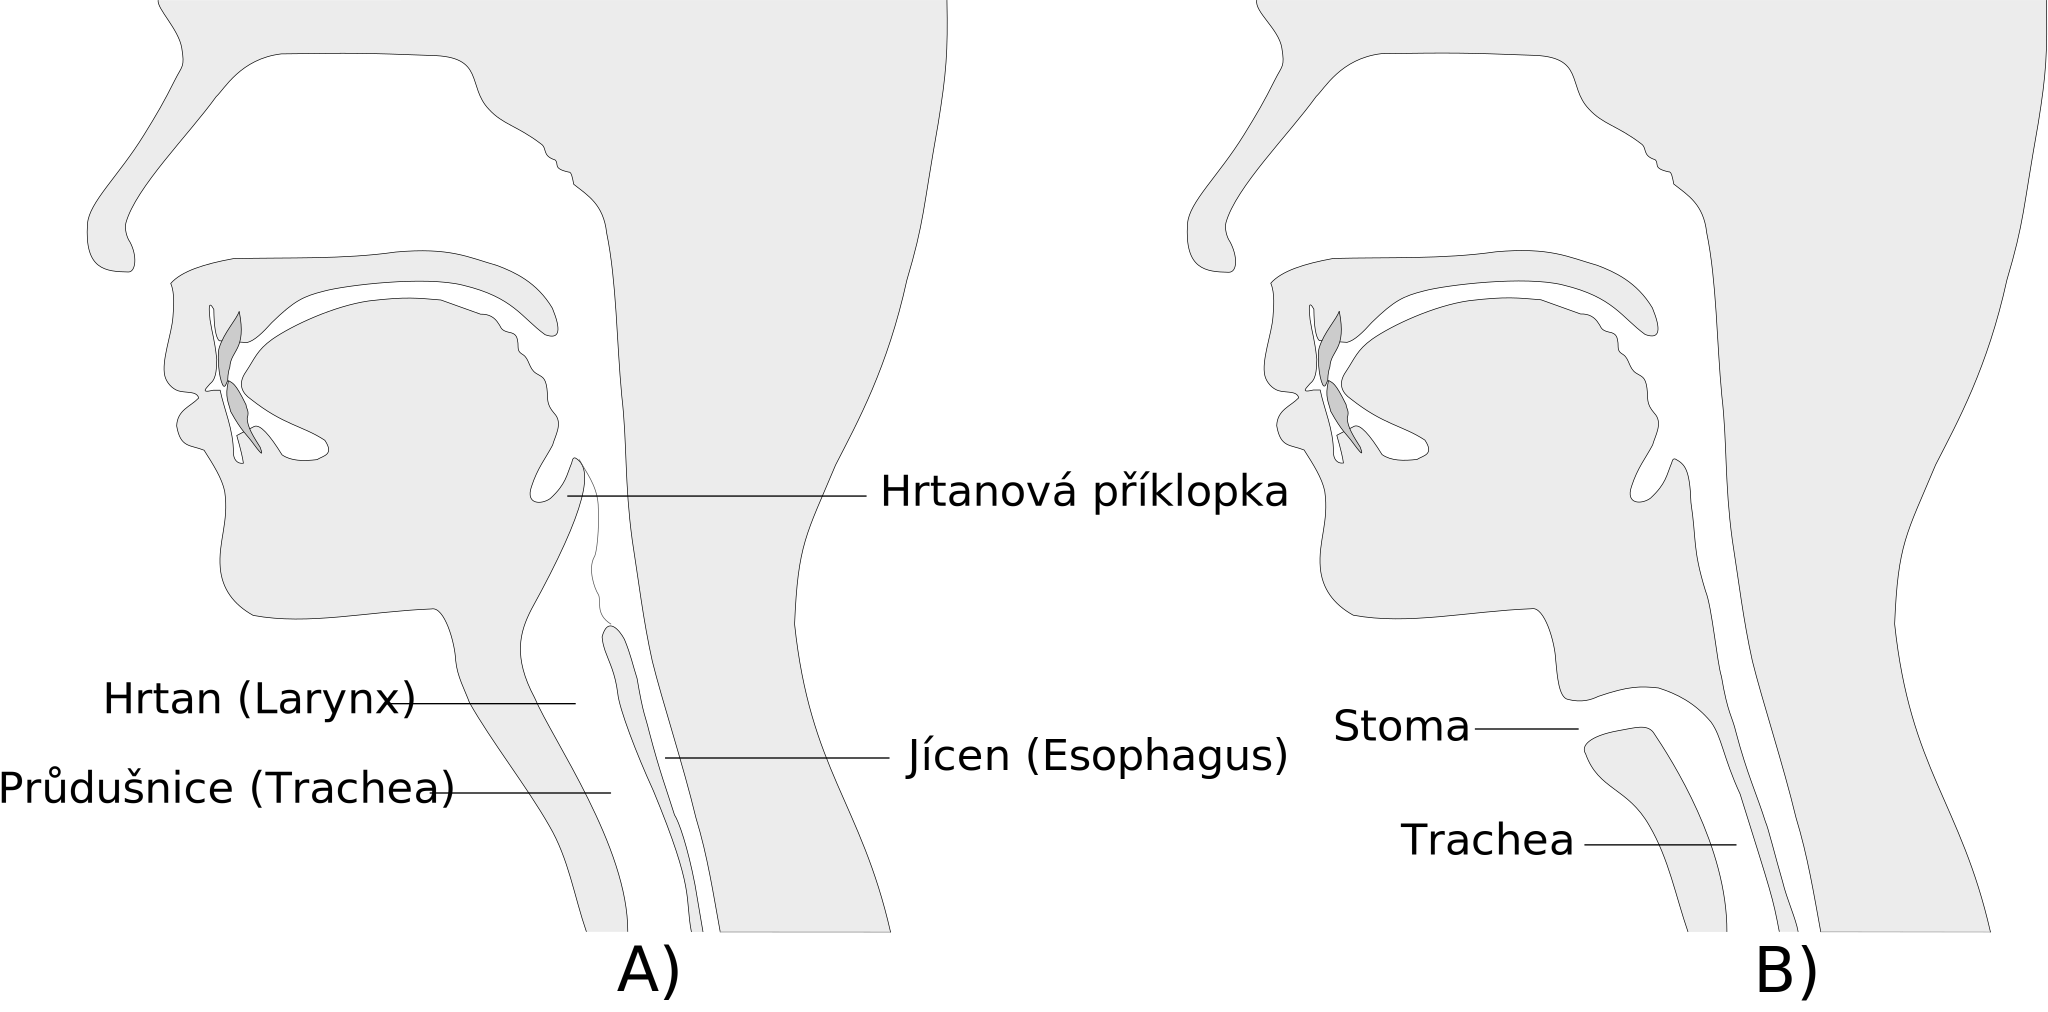
\includegraphics[width=0.9\linewidth]{ch3-cause/figures/dychaci-cesty-tl}
    \caption[Schéma dýchacích cest zdravého člověka (A) pacienta po totální laryngektomii (B)]{(A) Schéma dýchacích cest zdravého člověka (B) Schéma dýchacích cest po totální laryngektomii}
    \label{fig:cause:desease:laryngectomy}
  \end{center}
\end{figure}

Odstraněním spojení průdušnice a jícnu je zahrazena cesta vzduchu do plic.
Z~tohoto důvodu je nezbytné společně s TL vykonat také \textbf{tracheostomii}.
Cílem tohoto zákroku není léčba nádorovitého onemocnění, nýbrž vytvoření
vstupu pro vzduch směřující do plic a z~nich. Samotný zákrok se využívá i v
situacích, kdy dojde k uzávěře hrtanu a postižená osoba se dusí. K tomuto může
dojít například při alergické reakci na včelí bodnutí, otoku hrtanu, úrazu
apod. Při tracheostomii se provádí řez skrz kůži a průdušnici. Do vzniklého
otvoru se zavádí kanyla, která slouží k dýchání. Místo výkonu zákroku a
princip kanyly je znázorněn na obr. \ref{fig:cause:desease:tracheostomy}. Pro
lepší názornost je znázorněna tracheostomie se zavedenou kanylou u zdravého
člověka. Výsledek operace může být dočasný (například v případě alergické
reakce) nebo trvalý.

\begin{figure}[htb]
  \begin{center}
    \def\svgwidth{0.9\linewidth}
    % %LaTeX with PSTricks extensions
%%Creator: 0.48.3.1
%%Please note this file requires PSTricks extensions
\psset{xunit=.5pt,yunit=.5pt,runit=.5pt}
\begin{pspicture}(2907.24389648,1381.22814941)
{
\newrgbcolor{curcolor}{0.9254902 0.9254902 0.9254902}
\pscustom[linestyle=none,fillstyle=solid,fillcolor=curcolor]
{
\newpath
\moveto(70.56024,976.91215941)
\curveto(75.70194,998.05546941)(75.05233,1002.21845941)(63.72468,1022.97718941)
\curveto(59.11246,1029.25078941)(55.53152,1042.76249941)(57.82397,1051.05492941)
\curveto(72.33535,1103.54679941)(151.12483,1181.98458841)(191.6593,1238.29379441)
\curveto(203.82655,1249.22791741)(227.588336,1294.48932741)(288.348581,1301.70009441)
\curveto(395.40091,1303.19005241)(412.940729,1303.02200041)(510.35569,1299.36034741)
\curveto(591.16393,1298.04450341)(563.1446,1253.97868341)(596.12059,1219.46677821)
\curveto(617.11351,1196.64470041)(637.32731,1195.59050941)(673.24323,1168.28753341)
\curveto(683.09539,1161.70729041)(674.18628,1150.76886041)(694.17272,1144.46094641)
\curveto(700.8548,1138.26728041)(689.58524,1131.75588441)(714.56462,1126.38918541)
\curveto(718.47149,1127.09967441)(720.01648,1117.64831941)(721.82813,1108.38187941)
\curveto(742.89519,1091.67695941)(766.01459,1078.47903941)(770.6489,1036.21205941)
\curveto(785.52916,964.13363941)(785.41095,874.88456941)(793.05455,794.70262941)
\curveto(801.16608,725.36812941)(797.04543,665.20049941)(808.62059,580.55167941)
\curveto(817.99398,520.80324941)(824.99343,461.05482941)(838.33757,401.30639941)
\curveto(852.58351,343.43859941)(884.634,245.85682941)(902.96021,169.23090941)
\curveto(920.58527,111.57990941)(928.99355,58.22450941)(939.28097,2.24980941)
\lineto(1191.38979,0.50000941)
\curveto(1147.46289,192.92300941)(1072.39851,239.15118941)(1049.32187,456.03356941)
\curveto(1054.33227,575.87003941)(1066.33852,587.71091941)(1110.16719,692.25659941)
\curveto(1142.86475,756.08452941)(1187.16897,836.01858941)(1215.75173,966.06054941)
\curveto(1241.69732,1053.47858941)(1239.12891,1068.56755941)(1262.28051,1198.70444641)
\curveto(1274.15414,1272.24631941)(1276.84845,1302.56969941)(1275.20381,1380.20462941)
\curveto(1243.6598,1381.01350941)(132.01823,1379.13434941)(108.97269,1379.62040941)
\curveto(89.62734,1380.02842941)(136.091,1338.49754941)(140.67855,1310.22027841)
\curveto(145.31215,1281.65916741)(141.36641,1284.78090841)(130.36263,1262.73876141)
\curveto(114.38301,1230.72928461)(103.72405,1212.44353221)(84.57988,1181.51309641)
\curveto(46.3326,1119.71856941)(3.13314,1081.66825941)(0.88674,1049.70937941)
\curveto(-3.93696,981.08423941)(37.32565,977.54602941)(70.95213,976.84547941)
}
}
{
\newrgbcolor{curcolor}{0 0 0}
\pscustom[linewidth=1,linecolor=curcolor]
{
\newpath
\moveto(70.56024,976.91215941)
\curveto(75.70194,998.05546941)(75.05233,1002.21845941)(63.72468,1022.97718941)
\curveto(59.11246,1029.25078941)(55.53152,1042.76249941)(57.82397,1051.05492941)
\curveto(72.33535,1103.54679941)(151.12483,1181.98458841)(191.6593,1238.29379441)
\curveto(203.82655,1249.22791741)(227.588336,1294.48932741)(288.348581,1301.70009441)
\curveto(395.40091,1303.19005241)(412.940729,1303.02200041)(510.35569,1299.36034741)
\curveto(591.16393,1298.04450341)(563.1446,1253.97868341)(596.12059,1219.46677821)
\curveto(617.11351,1196.64470041)(637.32731,1195.59050941)(673.24323,1168.28753341)
\curveto(683.09539,1161.70729041)(674.18628,1150.76886041)(694.17272,1144.46094641)
\curveto(700.8548,1138.26728041)(689.58524,1131.75588441)(714.56462,1126.38918541)
\curveto(718.47149,1127.09967441)(720.01648,1117.64831941)(721.82813,1108.38187941)
\curveto(742.89519,1091.67695941)(766.01459,1078.47903941)(770.6489,1036.21205941)
\curveto(785.52916,964.13363941)(785.41095,874.88456941)(793.05455,794.70262941)
\curveto(801.16608,725.36812941)(797.04543,665.20049941)(808.62059,580.55167941)
\curveto(817.99398,520.80324941)(824.99343,461.05482941)(838.33757,401.30639941)
\curveto(852.58351,343.43859941)(884.634,245.85682941)(902.96021,169.23090941)
\curveto(920.58527,111.57990941)(928.99355,58.22450941)(939.28097,2.24980941)
\lineto(1191.38979,0.50000941)
\curveto(1147.46289,192.92300941)(1072.39851,239.15118941)(1049.32187,456.03356941)
\curveto(1054.33227,575.87003941)(1066.33852,587.71091941)(1110.16719,692.25659941)
\curveto(1142.86475,756.08452941)(1187.16897,836.01858941)(1215.75173,966.06054941)
\curveto(1241.69732,1053.47858941)(1239.12891,1068.56755941)(1262.28051,1198.70444641)
\curveto(1274.15414,1272.24631941)(1276.84845,1302.56969941)(1275.20381,1380.20462941)
\curveto(1243.6598,1381.01350941)(132.01823,1379.13434941)(108.97269,1379.62040941)
\curveto(89.62734,1380.02842941)(136.091,1338.49754941)(140.67855,1310.22027841)
\curveto(145.31215,1281.65916741)(141.36641,1284.78090841)(130.36263,1262.73876141)
\curveto(114.38301,1230.72928461)(103.72405,1212.44353221)(84.57988,1181.51309641)
\curveto(46.3326,1119.71856941)(3.13314,1081.66825941)(0.88674,1049.70937941)
\curveto(-3.93696,981.08423941)(37.32565,977.54602941)(70.95213,976.84547941)
}
}
{
\newrgbcolor{curcolor}{0.9254902 0.9254902 0.9254902}
\pscustom[linestyle=none,fillstyle=solid,fillcolor=curcolor]
{
\newpath
\moveto(663.80927,347.06111941)
\curveto(631.30672,407.78342941)(641.93353,444.78459941)(659.09229,478.19318941)
\curveto(742.49859,629.54060941)(751.64804,687.40579941)(724.24075,702.51595941)
\curveto(719.95848,704.09435941)(719.37506,696.51114941)(718.82765,695.21471941)
\curveto(711.30272,677.39364941)(710.58153,663.97482941)(687.1752,642.50022941)
\curveto(674.22342,633.07831941)(649.93085,632.99143941)(659.17482,660.02528941)
\curveto(668.2034,687.86169941)(679.75486,701.25992941)(690.49227,721.54170941)
\curveto(694.32384,735.78587941)(706.54118,754.42062941)(692.9595,768.66479941)
\curveto(680.15631,783.42381941)(684.07081,790.42534941)(682.11354,805.65799941)
\curveto(679.75193,823.26346941)(674.12318,822.66506941)(666.00743,828.02760941)
\curveto(655.05672,835.06925941)(656.16371,849.42328941)(646.73777,855.61704941)
\curveto(638.64629,860.32035941)(639.52383,863.34606941)(639.1639,872.76681941)
\curveto(637.98441,879.54741941)(638.28659,886.96301941)(625.74214,888.87292941)
\curveto(612.81159,891.73856941)(614.30292,897.00785941)(610.53081,901.39990941)
\curveto(604.8368,911.05283941)(596.12842,916.18422941)(583.68728,915.71645941)
\lineto(524.93857,936.77567941)
\curveto(490.25612,939.54036941)(474.30758,942.06391941)(418.15221,935.40170941)
\curveto(366.534745,928.00029941)(304.2199481,899.10557941)(274.750996,878.48752941)
\curveto(252.003981,862.15967941)(248.537062,849.31921941)(235.769747,830.34131941)
\curveto(222.937923,811.90137941)(230.373646,798.51614941)(242.774499,789.96747941)
\curveto(292.076635,750.86082941)(319.3103455,750.81408941)(352.832959,728.70655941)
\curveto(367.325625,706.91548941)(350.454946,706.03330941)(341.200769,700.07346941)
\curveto(321.2014438,697.73427941)(302.607692,697.85483941)(289.303279,707.23173941)
\curveto(270.762837,737.31808941)(256.564999,752.92908941)(248.143209,749.28659941)
\lineto(222.194469,735.86482941)
\curveto(228.231101,714.79611941)(231.053383,702.29899941)(232.037089,694.70475941)
\curveto(221.981864,693.29911941)(217.293619,701.68940941)(217.241359,710.28672941)
\curveto(217.477079,744.22373941)(203.2615,775.02108941)(197.55611,802.97364941)
\lineto(187.29789,802.97364941)
\curveto(166.56822,797.91572941)(178.05638,806.67132941)(182.82396,812.81626941)
\curveto(193.34887,820.71151941)(191.8352,839.37924941)(192.55804,848.77977941)
\curveto(189.01508,880.83561941)(186.10484,884.60710941)(182.56189,907.38269941)
\curveto(180.76794,924.17114941)(180.01497,937.66317941)(188.19267,922.87472941)
\curveto(188.49625,897.84202941)(190.8841,881.14644941)(196.24573,876.34594941)
\lineto(237.405799,873.66159941)
\curveto(248.143914,876.10038941)(260.863359,888.38046941)(274.091949,903.18947941)
\curveto(307.5567096,935.85866941)(321.1413212,942.22030941)(351.196907,949.82680941)
\curveto(383.523382,958.67919941)(501.87189,972.81484941)(557.73854,958.66609941)
\curveto(632.46539,940.77852941)(644.32636,910.80136941)(679.42919,885.29378941)
\curveto(701.57916,877.19347941)(703.43081,892.29125941)(690.1666,924.66429941)
\curveto(667.08021,963.46625941)(633.47421,978.37656941)(608.19846,987.93189941)
\curveto(565.49811,999.98699941)(539.14436,1015.15373941)(457.78478,1007.87922941)
\curveto(379.904483,996.64752941)(297.741184,1000.16294941)(216.825769,998.03659941)
\curveto(173.57623,990.17701941)(140.18925,979.41667941)(124.29082,961.33378941)
\curveto(130.726,946.56084941)(128.46979,924.48665941)(127.58388,911.82347941)
\curveto(125.77419,885.95569941)(110.07974,846.59298941)(115.57181,824.08208941)
\curveto(117.8965,814.55367941)(126.13355,805.09264941)(135.50065,802.07764941)
\curveto(146.31169,798.59789941)(163.07609,802.37811941)(165.7171,791.42292941)
\curveto(153.73391,778.74919941)(133.98029,773.84590941)(133.09836,750.07091941)
\curveto(138.68162,717.00597941)(153.29258,722.31734941)(173.72208,714.04142941)
\curveto(187.02623,693.18217941)(200.39377,672.31353941)(204.32814,652.84226941)
\curveto(210.9065,607.17595941)(194.37244,578.73022941)(197.73702,539.26597941)
\curveto(200.49791,508.68349941)(217.093467,485.47951941)(246.536796,469.12768941)
\curveto(327.687696,453.96820941)(416.73819,474.96141941)(510.92789,478.67598941)
\curveto(530.04251,482.78327941)(545.67914,429.27048941)(546.81162,402.15754941)
\curveto(549.12588,378.19912941)(560.21646,359.01453941)(567.26823,339.79363941)
\curveto(599.04903,283.26154941)(653.26269,213.99460941)(685.53957,157.14470941)
\curveto(714.54359,107.81710941)(724.30311,55.08410941)(742.45504,2.65910941)
\curveto(791.06479,2.93720941)(798.38877,2.65910941)(798.38877,2.65910941)
\curveto(799.22188,128.23700941)(690.30166,284.55155941)(663.80927,347.06111941)
\closepath
}
}
{
\newrgbcolor{curcolor}{0 0 0}
\pscustom[linewidth=1,linecolor=curcolor]
{
\newpath
\moveto(663.80927,347.06111941)
\curveto(631.30672,407.78342941)(641.93353,444.78459941)(659.09229,478.19318941)
\curveto(742.49859,629.54060941)(751.64804,687.40579941)(724.24075,702.51595941)
\curveto(719.95848,704.09435941)(719.37506,696.51114941)(718.82765,695.21471941)
\curveto(711.30272,677.39364941)(710.58153,663.97482941)(687.1752,642.50022941)
\curveto(674.22342,633.07831941)(649.93085,632.99143941)(659.17482,660.02528941)
\curveto(668.2034,687.86169941)(679.75486,701.25992941)(690.49227,721.54170941)
\curveto(694.32384,735.78587941)(706.54118,754.42062941)(692.9595,768.66479941)
\curveto(680.15631,783.42381941)(684.07081,790.42534941)(682.11354,805.65799941)
\curveto(679.75193,823.26346941)(674.12318,822.66506941)(666.00743,828.02760941)
\curveto(655.05672,835.06925941)(656.16371,849.42328941)(646.73777,855.61704941)
\curveto(638.64629,860.32035941)(639.52383,863.34606941)(639.1639,872.76681941)
\curveto(637.98441,879.54741941)(638.28659,886.96301941)(625.74214,888.87292941)
\curveto(612.81159,891.73856941)(614.30292,897.00785941)(610.53081,901.39990941)
\curveto(604.8368,911.05283941)(596.12842,916.18422941)(583.68728,915.71645941)
\lineto(524.93857,936.77567941)
\curveto(490.25612,939.54036941)(474.30758,942.06391941)(418.15221,935.40170941)
\curveto(366.534745,928.00029941)(304.2199481,899.10557941)(274.750996,878.48752941)
\curveto(252.003981,862.15967941)(248.537062,849.31921941)(235.769747,830.34131941)
\curveto(222.937923,811.90137941)(230.373646,798.51614941)(242.774499,789.96747941)
\curveto(292.076635,750.86082941)(319.3103455,750.81408941)(352.832959,728.70655941)
\curveto(367.325625,706.91548941)(350.454946,706.03330941)(341.200769,700.07346941)
\curveto(321.2014438,697.73427941)(302.607692,697.85483941)(289.303279,707.23173941)
\curveto(270.762837,737.31808941)(256.564999,752.92908941)(248.143209,749.28659941)
\lineto(222.194469,735.86482941)
\curveto(228.231101,714.79611941)(231.053383,702.29899941)(232.037089,694.70475941)
\curveto(221.981864,693.29911941)(217.293619,701.68940941)(217.241359,710.28672941)
\curveto(217.477079,744.22373941)(203.2615,775.02108941)(197.55611,802.97364941)
\lineto(187.29789,802.97364941)
\curveto(166.56822,797.91572941)(178.05638,806.67132941)(182.82396,812.81626941)
\curveto(193.34887,820.71151941)(191.8352,839.37924941)(192.55804,848.77977941)
\curveto(189.01508,880.83561941)(186.10484,884.60710941)(182.56189,907.38269941)
\curveto(180.76794,924.17114941)(180.01497,937.66317941)(188.19267,922.87472941)
\curveto(188.49625,897.84202941)(190.8841,881.14644941)(196.24573,876.34594941)
\lineto(237.405799,873.66159941)
\curveto(248.143914,876.10038941)(260.863359,888.38046941)(274.091949,903.18947941)
\curveto(307.5567096,935.85866941)(321.1413212,942.22030941)(351.196907,949.82680941)
\curveto(383.523382,958.67919941)(501.87189,972.81484941)(557.73854,958.66609941)
\curveto(632.46539,940.77852941)(644.32636,910.80136941)(679.42919,885.29378941)
\curveto(701.57916,877.19347941)(703.43081,892.29125941)(690.1666,924.66429941)
\curveto(667.08021,963.46625941)(633.47421,978.37656941)(608.19846,987.93189941)
\curveto(565.49811,999.98699941)(539.14436,1015.15373941)(457.78478,1007.87922941)
\curveto(379.904483,996.64752941)(297.741184,1000.16294941)(216.825769,998.03659941)
\curveto(173.57623,990.17701941)(140.18925,979.41667941)(124.29082,961.33378941)
\curveto(130.726,946.56084941)(128.46979,924.48665941)(127.58388,911.82347941)
\curveto(125.77419,885.95569941)(110.07974,846.59298941)(115.57181,824.08208941)
\curveto(117.8965,814.55367941)(126.13355,805.09264941)(135.50065,802.07764941)
\curveto(146.31169,798.59789941)(163.07609,802.37811941)(165.7171,791.42292941)
\curveto(153.73391,778.74919941)(133.98029,773.84590941)(133.09836,750.07091941)
\curveto(138.68162,717.00597941)(153.29258,722.31734941)(173.72208,714.04142941)
\curveto(187.02623,693.18217941)(200.39377,672.31353941)(204.32814,652.84226941)
\curveto(210.9065,607.17595941)(194.37244,578.73022941)(197.73702,539.26597941)
\curveto(200.49791,508.68349941)(217.093467,485.47951941)(246.536796,469.12768941)
\curveto(327.687696,453.96820941)(416.73819,474.96141941)(510.92789,478.67598941)
\curveto(530.04251,482.78327941)(545.67914,429.27048941)(546.81162,402.15754941)
\curveto(549.12588,378.19912941)(560.21646,359.01453941)(567.26823,339.79363941)
\curveto(599.04903,283.26154941)(653.26269,213.99460941)(685.53957,157.14470941)
\curveto(714.54359,107.81710941)(724.30311,55.08410941)(742.45504,2.65910941)
\curveto(791.06479,2.93720941)(798.38877,2.65910941)(798.38877,2.65910941)
\curveto(799.22188,128.23700941)(690.30166,284.55155941)(663.80927,347.06111941)
\closepath
}
}
{
\newrgbcolor{curcolor}{0.9254902 0.9254902 0.9254902}
\pscustom[linestyle=none,fillstyle=solid,fillcolor=curcolor]
{
\newpath
\moveto(895.41899,4.16750941)
\curveto(885.42628,56.53280941)(902.19573,58.71910941)(839.94237,209.07310941)
\curveto(814.28299,265.00824941)(789.33265,331.01818941)(787.1501,353.13337941)
\curveto(783.27094,384.03743941)(774.61723,398.97336941)(768.35964,416.66306941)
\curveto(765.06171,427.11926941)(764.824,429.14654941)(763.88572,437.24309941)
\curveto(772.18552,469.13804941)(790.10614,446.64287941)(796.99273,433.66395941)
\curveto(806.54018,410.67444941)(809.23317,396.02182941)(815.7832,375.50298941)
\curveto(825.27074,319.54128941)(827.96413,320.89590941)(833.67888,296.76197941)
\curveto(850.02247,234.61056941)(859.17548,212.00730941)(871.25982,173.28180941)
\curveto(877.50757,164.14560941)(890.91697,125.77240941)(901.68248,69.48680941)
\curveto(911.70975,10.97790941)(908.84075,23.55460941)(912.41989,3.27280941)
\closepath
}
}
{
\newrgbcolor{curcolor}{0 0 0}
\pscustom[linewidth=1,linecolor=curcolor]
{
\newpath
\moveto(895.41899,4.16750941)
\curveto(885.42628,56.53280941)(902.19573,58.71910941)(839.94237,209.07310941)
\curveto(814.28299,265.00824941)(789.33265,331.01818941)(787.1501,353.13337941)
\curveto(783.27094,384.03743941)(774.61723,398.97336941)(768.35964,416.66306941)
\curveto(765.06171,427.11926941)(764.824,429.14654941)(763.88572,437.24309941)
\curveto(772.18552,469.13804941)(790.10614,446.64287941)(796.99273,433.66395941)
\curveto(806.54018,410.67444941)(809.23317,396.02182941)(815.7832,375.50298941)
\curveto(825.27074,319.54128941)(827.96413,320.89590941)(833.67888,296.76197941)
\curveto(850.02247,234.61056941)(859.17548,212.00730941)(871.25982,173.28180941)
\curveto(877.50757,164.14560941)(890.91697,125.77240941)(901.68248,69.48680941)
\curveto(911.70975,10.97790941)(908.84075,23.55460941)(912.41989,3.27280941)
\closepath
}
}
{
\newrgbcolor{curcolor}{0.3019608 0.3019608 0.3019608}
\pscustom[linewidth=1,linecolor=curcolor]
{
\newpath
\moveto(777.30748,456.03356941)
\curveto(752.3253,471.35452941)(763.78475,491.53873941)(758.09534,500.48890941)
\curveto(752.61989,509.10247941)(742.51461,537.74873941)(752.25352,555.80199941)
\curveto(755.72774,560.13621941)(760.22549,596.01455941)(758.06962,633.64822941)
\curveto(756.02394,662.52158941)(739.67178,681.85842941)(729.88392,700.30964941)
}
}
{
\newrgbcolor{curcolor}{0.9254902 0.9254902 0.9254902}
\pscustom[linestyle=none,fillstyle=solid,fillcolor=curcolor]
{
\newpath
\moveto(1701.66159587,977.23068781)
\curveto(1706.80329587,998.37399781)(1706.15369587,1002.53698781)(1694.82599587,1023.29571781)
\curveto(1690.21379587,1029.56931781)(1686.63289587,1043.08102781)(1688.92529587,1051.37344781)
\curveto(1703.43669587,1103.86531781)(1782.22619587,1182.30311781)(1822.76069587,1238.61232781)
\curveto(1834.92789587,1249.54644781)(1858.68969587,1294.80786081)(1919.44989587,1302.01863081)
\curveto(2026.50229587,1303.50859081)(2044.04209587,1303.34053081)(2141.45699587,1299.67888081)
\curveto(2222.26529587,1298.36304081)(2194.24599587,1254.29721781)(2227.22189587,1219.78530781)
\curveto(2248.21489587,1196.96322781)(2268.42869587,1195.90903781)(2304.34459587,1168.60606781)
\curveto(2314.19669587,1162.02581781)(2305.28759587,1151.08738781)(2325.27409587,1144.77947781)
\curveto(2331.95619587,1138.58580781)(2320.68659587,1132.07441781)(2345.66599587,1126.70771781)
\curveto(2349.57279587,1127.41820781)(2351.11779587,1117.96683781)(2352.92949587,1108.70039781)
\curveto(2373.99649587,1091.99547781)(2397.11589587,1078.79755781)(2401.75029587,1036.53058781)
\curveto(2416.63049587,964.45216781)(2416.51229587,875.20310781)(2424.15589587,795.02115781)
\curveto(2432.26739587,725.68664781)(2428.14679587,665.51901781)(2439.72189587,580.87019781)
\curveto(2449.09529587,521.12176781)(2456.09479587,461.37334781)(2469.43889587,401.62491781)
\curveto(2483.68489587,343.75712781)(2515.73539587,246.17532781)(2534.06159587,169.54942781)
\curveto(2551.68659587,111.89842781)(2560.09489587,58.54302781)(2570.38229587,2.56832781)
\lineto(2822.49109587,0.81852781)
\curveto(2778.56419587,193.24152781)(2703.49979587,239.46972781)(2680.42319587,456.35208781)
\curveto(2685.43359587,576.18855781)(2697.43979587,588.02943781)(2741.26849587,692.57511781)
\curveto(2773.96599587,756.40305781)(2818.27029587,836.33711781)(2846.85299587,966.37907781)
\curveto(2872.79859587,1053.79710781)(2870.23019587,1068.88607781)(2893.38179587,1199.02297781)
\curveto(2905.25539587,1272.56484781)(2907.94969587,1302.88823081)(2906.30509587,1380.5231509)
\curveto(2874.76109587,1381.3320309)(1763.11959587,1379.45287091)(1740.07399587,1379.9389309)
\curveto(1720.72869587,1380.3469509)(1767.19239587,1338.81607081)(1771.77989587,1310.53881081)
\curveto(1776.41349587,1281.97770081)(1772.46779587,1285.09944081)(1761.46399587,1263.05728781)
\curveto(1745.48439587,1231.04781781)(1734.82539587,1212.76205781)(1715.68119587,1181.83162781)
\curveto(1677.43399587,1120.03708781)(1634.23449587,1081.98677781)(1631.98809587,1050.02789781)
\curveto(1627.16439587,981.40276781)(1668.42699587,977.86455781)(1702.05349587,977.16400781)
}
}
{
\newrgbcolor{curcolor}{0 0 0}
\pscustom[linewidth=1,linecolor=curcolor]
{
\newpath
\moveto(1701.66159587,977.23068781)
\curveto(1706.80329587,998.37399781)(1706.15369587,1002.53698781)(1694.82599587,1023.29571781)
\curveto(1690.21379587,1029.56931781)(1686.63289587,1043.08102781)(1688.92529587,1051.37344781)
\curveto(1703.43669587,1103.86531781)(1782.22619587,1182.30311781)(1822.76069587,1238.61232781)
\curveto(1834.92789587,1249.54644781)(1858.68969587,1294.80786081)(1919.44989587,1302.01863081)
\curveto(2026.50229587,1303.50859081)(2044.04209587,1303.34053081)(2141.45699587,1299.67888081)
\curveto(2222.26529587,1298.36304081)(2194.24599587,1254.29721781)(2227.22189587,1219.78530781)
\curveto(2248.21489587,1196.96322781)(2268.42869587,1195.90903781)(2304.34459587,1168.60606781)
\curveto(2314.19669587,1162.02581781)(2305.28759587,1151.08738781)(2325.27409587,1144.77947781)
\curveto(2331.95619587,1138.58580781)(2320.68659587,1132.07441781)(2345.66599587,1126.70771781)
\curveto(2349.57279587,1127.41820781)(2351.11779587,1117.96683781)(2352.92949587,1108.70039781)
\curveto(2373.99649587,1091.99547781)(2397.11589587,1078.79755781)(2401.75029587,1036.53058781)
\curveto(2416.63049587,964.45216781)(2416.51229587,875.20310781)(2424.15589587,795.02115781)
\curveto(2432.26739587,725.68664781)(2428.14679587,665.51901781)(2439.72189587,580.87019781)
\curveto(2449.09529587,521.12176781)(2456.09479587,461.37334781)(2469.43889587,401.62491781)
\curveto(2483.68489587,343.75712781)(2515.73539587,246.17532781)(2534.06159587,169.54942781)
\curveto(2551.68659587,111.89842781)(2560.09489587,58.54302781)(2570.38229587,2.56832781)
\lineto(2822.49109587,0.81852781)
\curveto(2778.56419587,193.24152781)(2703.49979587,239.46972781)(2680.42319587,456.35208781)
\curveto(2685.43359587,576.18855781)(2697.43979587,588.02943781)(2741.26849587,692.57511781)
\curveto(2773.96599587,756.40305781)(2818.27029587,836.33711781)(2846.85299587,966.37907781)
\curveto(2872.79859587,1053.79710781)(2870.23019587,1068.88607781)(2893.38179587,1199.02297781)
\curveto(2905.25539587,1272.56484781)(2907.94969587,1302.88823081)(2906.30509587,1380.5231509)
\curveto(2874.76109587,1381.3320309)(1763.11959587,1379.45287091)(1740.07399587,1379.9389309)
\curveto(1720.72869587,1380.3469509)(1767.19239587,1338.81607081)(1771.77989587,1310.53881081)
\curveto(1776.41349587,1281.97770081)(1772.46779587,1285.09944081)(1761.46399587,1263.05728781)
\curveto(1745.48439587,1231.04781781)(1734.82539587,1212.76205781)(1715.68119587,1181.83162781)
\curveto(1677.43399587,1120.03708781)(1634.23449587,1081.98677781)(1631.98809587,1050.02789781)
\curveto(1627.16439587,981.40276781)(1668.42699587,977.86455781)(1702.05349587,977.16400781)
}
}
{
\newrgbcolor{curcolor}{0.9254902 0.9254902 0.9254902}
\pscustom[linestyle=none,fillstyle=solid,fillcolor=curcolor]
{
\newpath
\moveto(2222.18449587,263.90192781)
\curveto(2241.31109587,209.90072781)(2284.36399587,214.31312781)(2316.64089587,157.46322781)
\curveto(2345.64489587,108.13562781)(2355.40449587,55.40262781)(2373.55639587,2.97762781)
\curveto(2422.16609587,3.25572781)(2429.49009587,2.97762781)(2429.49009587,2.97762781)
\curveto(2430.32319587,128.55552781)(2351.03939587,253.41772781)(2322.64889587,295.68062781)
\curveto(2312.63549587,308.42372781)(2295.39239587,302.39362781)(2270.51859587,298.13982781)
\curveto(2228.12249587,290.36432781)(2214.62639587,275.73032781)(2222.18449587,263.90192781)
\closepath
\moveto(2241.02189587,349.02342781)
\curveto(2285.97709587,364.43132781)(2303.47489587,364.38192781)(2330.30379587,361.55452781)
\curveto(2357.48059587,352.76802781)(2383.60959587,340.11422781)(2408.12809587,311.06042781)
\curveto(2424.23029587,288.94522781)(2445.38429587,265.32672781)(2471.04369587,209.39162781)
\curveto(2533.29709587,59.03762781)(2516.52759587,56.85132781)(2526.52029587,4.48602781)
\lineto(2543.52119587,3.59132781)
\curveto(2539.94209587,23.87312781)(2542.81109587,11.29642781)(2532.78379587,69.80532781)
\curveto(2522.01829587,126.09092781)(2508.60889587,164.46412781)(2502.36119587,173.60032781)
\curveto(2490.27679587,212.32582781)(2481.12379587,234.92902781)(2464.78019587,297.08052781)
\curveto(2459.06549587,321.21442781)(2456.37209587,319.85982781)(2446.88459587,375.82152781)
\curveto(2440.33449587,396.34034781)(2416.76219587,481.22354781)(2407.21469587,504.21305781)
\curveto(2387.67399587,567.80861781)(2386.83649587,580.18045781)(2378.38959587,636.46615781)
\curveto(2376.77379587,686.52617781)(2369.04569587,693.38127781)(2355.34209587,700.93635781)
\curveto(2351.05979587,702.51475781)(2350.47639587,696.82966781)(2349.92899587,695.53323781)
\curveto(2342.40409587,677.71216781)(2341.68289587,664.29334781)(2318.27659587,642.81874781)
\curveto(2305.32479587,633.39683781)(2281.03219587,633.30995781)(2290.27619587,660.34380781)
\curveto(2299.30479587,688.18021781)(2310.85619587,701.57844781)(2321.59359587,721.86022781)
\curveto(2325.42519587,736.10439781)(2337.64249587,754.73915781)(2324.06089587,768.98332781)
\curveto(2311.25769587,783.74234781)(2315.17219587,790.74387781)(2313.21489587,805.97652781)
\curveto(2310.85329587,823.58199781)(2305.22449587,822.98359781)(2297.10879587,828.34613781)
\curveto(2286.15809587,835.38778781)(2287.26509587,849.74182781)(2277.83909587,855.93558781)
\curveto(2269.74759587,860.63889781)(2270.62519587,863.66460781)(2270.26529587,873.08535781)
\curveto(2269.08579587,879.86595781)(2269.38789587,887.28155781)(2256.84349587,889.19146781)
\curveto(2243.91289587,892.05710781)(2245.40429587,897.32639781)(2241.63219587,901.71844781)
\curveto(2235.93819587,911.37137781)(2227.22979587,916.50276781)(2214.78859587,916.03499781)
\lineto(2156.03989587,937.09421781)
\curveto(2121.35749587,939.85890781)(2105.40889587,942.38245781)(2049.25359587,935.72024781)
\curveto(1997.63609587,928.31883781)(1935.32129587,899.42411781)(1905.85229587,878.80606781)
\curveto(1883.10529587,862.47821781)(1879.63839587,849.63775781)(1866.87109587,830.65984781)
\curveto(1854.03929587,812.21990781)(1861.47499587,798.83467781)(1873.87579587,790.28600781)
\curveto(1923.17799587,751.17934781)(1950.41169587,751.13260781)(1983.93429587,729.02507781)
\curveto(1998.42699587,707.23400781)(1981.55629587,706.35182781)(1972.30209587,700.39198781)
\curveto(1952.30279587,698.05279781)(1933.70899587,698.17335781)(1920.40459587,707.55025781)
\curveto(1901.86419587,737.63660781)(1887.66629587,753.24760781)(1879.24459587,749.60511781)
\lineto(1853.29579587,736.18334781)
\curveto(1859.33249587,715.11463781)(1862.15469587,702.61751781)(1863.13839587,695.02327781)
\curveto(1853.08319587,693.61763781)(1848.39499587,702.00792781)(1848.34269587,710.60524781)
\curveto(1848.57839587,744.54225781)(1834.36289587,775.33961781)(1828.65749587,803.29217781)
\lineto(1818.39919587,803.29217781)
\curveto(1797.66959587,798.23425781)(1809.15769587,806.98985781)(1813.92529587,813.13479781)
\curveto(1824.45019587,821.03004781)(1822.93659587,839.69777781)(1823.65939587,849.09831781)
\curveto(1820.11639587,881.15415781)(1817.20619587,884.92564781)(1813.66319587,907.70123781)
\curveto(1811.86929587,924.48968781)(1811.11629587,937.98171781)(1819.29399587,923.19326781)
\curveto(1819.59759587,898.16056781)(1821.98549587,881.46498781)(1827.34709587,876.66448781)
\lineto(1868.50709587,873.98013781)
\curveto(1879.24529587,876.41892781)(1891.96469587,888.69900781)(1905.19329587,903.50801781)
\curveto(1938.65809587,936.17720781)(1952.24269587,942.53884781)(1982.29829587,950.14534781)
\curveto(2014.62469587,958.99772781)(2132.97319587,973.13337781)(2188.83989587,958.98462781)
\curveto(2263.56669587,941.09706781)(2275.42769587,911.11990781)(2310.53049587,885.61232781)
\curveto(2332.68049587,877.51201781)(2334.53219587,892.60979781)(2321.26799587,924.98283781)
\curveto(2298.18159587,963.78478781)(2264.57559587,978.69509781)(2239.29979587,988.25042781)
\curveto(2196.59949587,1000.30552781)(2170.24569587,1015.47226781)(2088.88609587,1008.19775781)
\curveto(2011.00579587,996.96605781)(1928.84249587,1000.48147781)(1847.92709587,998.35512781)
\curveto(1804.67759587,990.49554781)(1771.29059587,979.73520781)(1755.39219587,961.65231781)
\curveto(1761.82739587,946.87938781)(1759.57109587,924.80519781)(1758.68519587,912.14201781)
\curveto(1756.87549587,886.27423781)(1741.18109587,846.91151781)(1746.67319587,824.40061781)
\curveto(1748.99789587,814.87220781)(1757.23489587,805.41117781)(1766.60199587,802.39617781)
\curveto(1777.41299587,798.91642781)(1794.17739587,802.69664781)(1796.81849587,791.74145781)
\curveto(1784.83529587,779.06772781)(1765.08159587,774.16443781)(1764.19969587,750.38943781)
\curveto(1769.78299587,717.32449781)(1784.39389587,722.63586781)(1804.82339587,714.35994781)
\curveto(1818.12759587,693.50069781)(1831.49509587,672.63205781)(1835.42949587,653.16078781)
\curveto(1842.00789587,607.49447781)(1825.47379587,579.04874781)(1828.83839587,539.58449781)
\curveto(1831.59929587,509.00201781)(1848.19479587,485.79803781)(1877.63809587,469.44620781)
\curveto(1958.78899587,454.28672781)(2047.83949587,475.27993781)(2142.02919587,478.99450781)
\curveto(2161.14389587,483.10179781)(2176.78049587,429.58900781)(2177.91299587,402.47606781)
\curveto(2180.22719587,378.51762781)(2182.50489587,347.35652781)(2195.88369587,344.58602781)
\curveto(2216.40419587,339.36112781)(2230.61569587,343.95892781)(2241.02189587,349.02342781)
\closepath
}
}
{
\newrgbcolor{curcolor}{0 0 0}
\pscustom[linewidth=1,linecolor=curcolor]
{
\newpath
\moveto(2222.18449587,263.90192781)
\curveto(2241.31109587,209.90072781)(2284.36399587,214.31312781)(2316.64089587,157.46322781)
\curveto(2345.64489587,108.13562781)(2355.40449587,55.40262781)(2373.55639587,2.97762781)
\curveto(2422.16609587,3.25572781)(2429.49009587,2.97762781)(2429.49009587,2.97762781)
\curveto(2430.32319587,128.55552781)(2351.03939587,253.41772781)(2322.64889587,295.68062781)
\curveto(2312.63549587,308.42372781)(2295.39239587,302.39362781)(2270.51859587,298.13982781)
\curveto(2228.12249587,290.36432781)(2214.62639587,275.73032781)(2222.18449587,263.90192781)
\closepath
\moveto(2241.02189587,349.02342781)
\curveto(2285.97709587,364.43132781)(2303.47489587,364.38192781)(2330.30379587,361.55452781)
\curveto(2357.48059587,352.76802781)(2383.60959587,340.11422781)(2408.12809587,311.06042781)
\curveto(2424.23029587,288.94522781)(2445.38429587,265.32672781)(2471.04369587,209.39162781)
\curveto(2533.29709587,59.03762781)(2516.52759587,56.85132781)(2526.52029587,4.48602781)
\lineto(2543.52119587,3.59132781)
\curveto(2539.94209587,23.87312781)(2542.81109587,11.29642781)(2532.78379587,69.80532781)
\curveto(2522.01829587,126.09092781)(2508.60889587,164.46412781)(2502.36119587,173.60032781)
\curveto(2490.27679587,212.32582781)(2481.12379587,234.92902781)(2464.78019587,297.08052781)
\curveto(2459.06549587,321.21442781)(2456.37209587,319.85982781)(2446.88459587,375.82152781)
\curveto(2440.33449587,396.34034781)(2416.76219587,481.22354781)(2407.21469587,504.21305781)
\curveto(2387.67399587,567.80861781)(2386.83649587,580.18045781)(2378.38959587,636.46615781)
\curveto(2376.77379587,686.52617781)(2369.04569587,693.38127781)(2355.34209587,700.93635781)
\curveto(2351.05979587,702.51475781)(2350.47639587,696.82966781)(2349.92899587,695.53323781)
\curveto(2342.40409587,677.71216781)(2341.68289587,664.29334781)(2318.27659587,642.81874781)
\curveto(2305.32479587,633.39683781)(2281.03219587,633.30995781)(2290.27619587,660.34380781)
\curveto(2299.30479587,688.18021781)(2310.85619587,701.57844781)(2321.59359587,721.86022781)
\curveto(2325.42519587,736.10439781)(2337.64249587,754.73915781)(2324.06089587,768.98332781)
\curveto(2311.25769587,783.74234781)(2315.17219587,790.74387781)(2313.21489587,805.97652781)
\curveto(2310.85329587,823.58199781)(2305.22449587,822.98359781)(2297.10879587,828.34613781)
\curveto(2286.15809587,835.38778781)(2287.26509587,849.74182781)(2277.83909587,855.93558781)
\curveto(2269.74759587,860.63889781)(2270.62519587,863.66460781)(2270.26529587,873.08535781)
\curveto(2269.08579587,879.86595781)(2269.38789587,887.28155781)(2256.84349587,889.19146781)
\curveto(2243.91289587,892.05710781)(2245.40429587,897.32639781)(2241.63219587,901.71844781)
\curveto(2235.93819587,911.37137781)(2227.22979587,916.50276781)(2214.78859587,916.03499781)
\lineto(2156.03989587,937.09421781)
\curveto(2121.35749587,939.85890781)(2105.40889587,942.38245781)(2049.25359587,935.72024781)
\curveto(1997.63609587,928.31883781)(1935.32129587,899.42411781)(1905.85229587,878.80606781)
\curveto(1883.10529587,862.47821781)(1879.63839587,849.63775781)(1866.87109587,830.65984781)
\curveto(1854.03929587,812.21990781)(1861.47499587,798.83467781)(1873.87579587,790.28600781)
\curveto(1923.17799587,751.17934781)(1950.41169587,751.13260781)(1983.93429587,729.02507781)
\curveto(1998.42699587,707.23400781)(1981.55629587,706.35182781)(1972.30209587,700.39198781)
\curveto(1952.30279587,698.05279781)(1933.70899587,698.17335781)(1920.40459587,707.55025781)
\curveto(1901.86419587,737.63660781)(1887.66629587,753.24760781)(1879.24459587,749.60511781)
\lineto(1853.29579587,736.18334781)
\curveto(1859.33249587,715.11463781)(1862.15469587,702.61751781)(1863.13839587,695.02327781)
\curveto(1853.08319587,693.61763781)(1848.39499587,702.00792781)(1848.34269587,710.60524781)
\curveto(1848.57839587,744.54225781)(1834.36289587,775.33961781)(1828.65749587,803.29217781)
\lineto(1818.39919587,803.29217781)
\curveto(1797.66959587,798.23425781)(1809.15769587,806.98985781)(1813.92529587,813.13479781)
\curveto(1824.45019587,821.03004781)(1822.93659587,839.69777781)(1823.65939587,849.09831781)
\curveto(1820.11639587,881.15415781)(1817.20619587,884.92564781)(1813.66319587,907.70123781)
\curveto(1811.86929587,924.48968781)(1811.11629587,937.98171781)(1819.29399587,923.19326781)
\curveto(1819.59759587,898.16056781)(1821.98549587,881.46498781)(1827.34709587,876.66448781)
\lineto(1868.50709587,873.98013781)
\curveto(1879.24529587,876.41892781)(1891.96469587,888.69900781)(1905.19329587,903.50801781)
\curveto(1938.65809587,936.17720781)(1952.24269587,942.53884781)(1982.29829587,950.14534781)
\curveto(2014.62469587,958.99772781)(2132.97319587,973.13337781)(2188.83989587,958.98462781)
\curveto(2263.56669587,941.09706781)(2275.42769587,911.11990781)(2310.53049587,885.61232781)
\curveto(2332.68049587,877.51201781)(2334.53219587,892.60979781)(2321.26799587,924.98283781)
\curveto(2298.18159587,963.78478781)(2264.57559587,978.69509781)(2239.29979587,988.25042781)
\curveto(2196.59949587,1000.30552781)(2170.24569587,1015.47226781)(2088.88609587,1008.19775781)
\curveto(2011.00579587,996.96605781)(1928.84249587,1000.48147781)(1847.92709587,998.35512781)
\curveto(1804.67759587,990.49554781)(1771.29059587,979.73520781)(1755.39219587,961.65231781)
\curveto(1761.82739587,946.87938781)(1759.57109587,924.80519781)(1758.68519587,912.14201781)
\curveto(1756.87549587,886.27423781)(1741.18109587,846.91151781)(1746.67319587,824.40061781)
\curveto(1748.99789587,814.87220781)(1757.23489587,805.41117781)(1766.60199587,802.39617781)
\curveto(1777.41299587,798.91642781)(1794.17739587,802.69664781)(1796.81849587,791.74145781)
\curveto(1784.83529587,779.06772781)(1765.08159587,774.16443781)(1764.19969587,750.38943781)
\curveto(1769.78299587,717.32449781)(1784.39389587,722.63586781)(1804.82339587,714.35994781)
\curveto(1818.12759587,693.50069781)(1831.49509587,672.63205781)(1835.42949587,653.16078781)
\curveto(1842.00789587,607.49447781)(1825.47379587,579.04874781)(1828.83839587,539.58449781)
\curveto(1831.59929587,509.00201781)(1848.19479587,485.79803781)(1877.63809587,469.44620781)
\curveto(1958.78899587,454.28672781)(2047.83949587,475.27993781)(2142.02919587,478.99450781)
\curveto(2161.14389587,483.10179781)(2176.78049587,429.58900781)(2177.91299587,402.47606781)
\curveto(2180.22719587,378.51762781)(2182.50489587,347.35652781)(2195.88369587,344.58602781)
\curveto(2216.40419587,339.36112781)(2230.61569587,343.95892781)(2241.02189587,349.02342781)
\closepath
}
}
{
\newrgbcolor{curcolor}{0.80000001 0.80000001 0.80000001}
\pscustom[linestyle=none,fillstyle=solid,fillcolor=curcolor]
{
\newpath
\moveto(1856.91629587,920.33095781)
\curveto(1852.97789587,908.04444781)(1834.19749587,888.87896781)(1827.17899587,865.91806781)
\curveto(1825.13979587,861.15995781)(1825.04509587,833.60610781)(1830.34249587,816.56683781)
\curveto(1835.47639587,800.05400781)(1837.88419587,815.66513781)(1839.83319587,817.19954781)
\curveto(1840.15089587,828.36895781)(1841.50219587,833.33705781)(1842.99669587,837.44620781)
\curveto(1844.41779587,863.38058781)(1868.34079587,862.30071781)(1856.91629587,920.33095781)
\closepath
}
}
{
\newrgbcolor{curcolor}{0 0 0}
\pscustom[linewidth=1,linecolor=curcolor]
{
\newpath
\moveto(1856.91629587,920.33095781)
\curveto(1852.97789587,908.04444781)(1834.19749587,888.87896781)(1827.17899587,865.91806781)
\curveto(1825.13979587,861.15995781)(1825.04509587,833.60610781)(1830.34249587,816.56683781)
\curveto(1835.47639587,800.05400781)(1837.88419587,815.66513781)(1839.83319587,817.19954781)
\curveto(1840.15089587,828.36895781)(1841.50219587,833.33705781)(1842.99669587,837.44620781)
\curveto(1844.41779587,863.38058781)(1868.34079587,862.30071781)(1856.91629587,920.33095781)
\closepath
}
}
{
\newrgbcolor{curcolor}{0.80000001 0.80000001 0.80000001}
\pscustom[linestyle=none,fillstyle=solid,fillcolor=curcolor]
{
\newpath
\moveto(1841.06769587,817.50097781)
\curveto(1834.91779587,792.39807781)(1841.57179587,784.90070781)(1844.19949587,771.86697781)
\curveto(1861.53959587,740.38321781)(1867.17519587,739.33153781)(1878.64859587,723.10122781)
\curveto(1894.86219587,701.16965781)(1890.18049587,711.88679781)(1888.04389587,718.62730781)
\curveto(1878.82579587,733.44367781)(1868.79449587,748.36168781)(1868.80599587,762.02435781)
\curveto(1872.25039587,772.62703781)(1867.57169587,775.10654781)(1867.01649587,781.70960781)
\curveto(1850.58659587,815.68321781)(1846.85249587,813.68698781)(1841.06769587,817.50097781)
\closepath
}
}
{
\newrgbcolor{curcolor}{0 0 0}
\pscustom[linewidth=1,linecolor=curcolor]
{
\newpath
\moveto(1841.06769587,817.50097781)
\curveto(1834.91779587,792.39807781)(1841.57179587,784.90070781)(1844.19949587,771.86697781)
\curveto(1861.53959587,740.38321781)(1867.17519587,739.33153781)(1878.64859587,723.10122781)
\curveto(1894.86219587,701.16965781)(1890.18049587,711.88679781)(1888.04389587,718.62730781)
\curveto(1878.82579587,733.44367781)(1868.79449587,748.36168781)(1868.80599587,762.02435781)
\curveto(1872.25039587,772.62703781)(1867.57169587,775.10654781)(1867.01649587,781.70960781)
\curveto(1850.58659587,815.68321781)(1846.85249587,813.68698781)(1841.06769587,817.50097781)
\closepath
}
}
{
\newrgbcolor{curcolor}{0.80000001 0.80000001 0.80000001}
\pscustom[linestyle=none,fillstyle=solid,fillcolor=curcolor]
{
\newpath
\moveto(225.814918,920.01241941)
\curveto(221.876528,907.72590941)(203.09611,888.56042941)(196.07765,865.59952941)
\curveto(194.03846,860.84141941)(193.9437,833.28757941)(199.24119,816.24830941)
\curveto(204.37501,799.73547941)(206.78283,815.34660941)(208.73181,816.88101941)
\curveto(209.04957,828.05042941)(210.40088,833.01852941)(211.89535,837.12767941)
\curveto(213.31641,863.06204941)(237.239466,861.98217941)(225.814918,920.01241941)
\closepath
}
}
{
\newrgbcolor{curcolor}{0 0 0}
\pscustom[linewidth=1,linecolor=curcolor]
{
\newpath
\moveto(225.814918,920.01241941)
\curveto(221.876528,907.72590941)(203.09611,888.56042941)(196.07765,865.59952941)
\curveto(194.03846,860.84141941)(193.9437,833.28757941)(199.24119,816.24830941)
\curveto(204.37501,799.73547941)(206.78283,815.34660941)(208.73181,816.88101941)
\curveto(209.04957,828.05042941)(210.40088,833.01852941)(211.89535,837.12767941)
\curveto(213.31641,863.06204941)(237.239466,861.98217941)(225.814918,920.01241941)
\closepath
}
}
{
\newrgbcolor{curcolor}{0.80000001 0.80000001 0.80000001}
\pscustom[linestyle=none,fillstyle=solid,fillcolor=curcolor]
{
\newpath
\moveto(209.96636,817.18244941)
\curveto(203.81641,792.07954941)(210.47048,784.58217941)(213.09811,771.54844941)
\curveto(230.438288,740.06469941)(236.073825,739.01301941)(247.547296,722.78270941)
\curveto(263.760808,700.85113941)(259.079151,711.56827941)(256.94253,718.30878941)
\curveto(247.724425,733.12515941)(237.693145,748.04316941)(237.70467,761.70582941)
\curveto(241.149079,772.30850941)(236.47031,774.78801941)(235.915102,781.39107941)
\curveto(219.485298,815.36468941)(215.751198,813.36845941)(209.96636,817.18244941)
\closepath
}
}
{
\newrgbcolor{curcolor}{0 0 0}
\pscustom[linewidth=1,linecolor=curcolor]
{
\newpath
\moveto(209.96636,817.18244941)
\curveto(203.81641,792.07954941)(210.47048,784.58217941)(213.09811,771.54844941)
\curveto(230.438288,740.06469941)(236.073825,739.01301941)(247.547296,722.78270941)
\curveto(263.760808,700.85113941)(259.079151,711.56827941)(256.94253,718.30878941)
\curveto(247.724425,733.12515941)(237.693145,748.04316941)(237.70467,761.70582941)
\curveto(241.149079,772.30850941)(236.47031,774.78801941)(235.915102,781.39107941)
\curveto(219.485298,815.36468941)(215.751198,813.36845941)(209.96636,817.18244941)
\closepath
}
}
{
\newrgbcolor{curcolor}{0 0 0}
\pscustom[linestyle=none,fillstyle=solid,fillcolor=curcolor]
{
\newpath
\moveto(35.93132134,187.90693012)
\lineto(35.93132134,222.26630512)
\lineto(48.89225884,222.26630512)
\curveto(51.17348989,222.26627076)(52.91567565,222.15689587)(54.11882134,221.93818012)
\curveto(55.80629776,221.65689637)(57.22035885,221.12174066)(58.36100884,220.33271137)
\curveto(59.50160656,219.54361724)(60.4195744,218.43814959)(61.11491509,217.01630512)
\curveto(61.81019801,215.59440243)(62.15785391,214.031904)(62.15788384,212.32880512)
\curveto(62.15785391,209.40690862)(61.22816734,206.93425484)(59.36882134,204.91083637)
\curveto(57.50942106,202.88738389)(54.15004942,201.87566615)(49.29069634,201.87568012)
\lineto(40.47819634,201.87568012)
\lineto(40.47819634,187.90693012)
\closepath
\moveto(40.47819634,205.93036762)
\lineto(49.36100884,205.93036762)
\curveto(52.29848877,205.9303496)(54.38442418,206.47722405)(55.61882134,207.57099262)
\curveto(56.85317171,208.66472186)(57.4703586,210.20378282)(57.47038384,212.18818012)
\curveto(57.4703586,213.6256544)(57.10707771,214.85612192)(56.38054009,215.87958637)
\curveto(55.65395416,216.90299488)(54.69692387,217.57877545)(53.50944634,217.90693012)
\curveto(52.74380082,218.11002492)(51.32973974,218.21158732)(49.26725884,218.21161762)
\lineto(40.47819634,218.21161762)
\closepath
}
}
{
\newrgbcolor{curcolor}{0 0 0}
\pscustom[linestyle=none,fillstyle=solid,fillcolor=curcolor]
{
\newpath
\moveto(67.40788384,187.90693012)
\lineto(67.40788384,212.79755512)
\lineto(71.20475884,212.79755512)
\lineto(71.20475884,209.02411762)
\curveto(72.17350095,210.78971974)(73.06803131,211.95378107)(73.88835259,212.51630512)
\curveto(74.70865467,213.07877995)(75.61099752,213.36002967)(76.59538384,213.36005512)
\curveto(78.01724511,213.36002967)(79.46255617,212.90690512)(80.93132134,212.00068012)
\lineto(79.47819634,208.08661762)
\curveto(78.44693218,208.69597183)(77.41568321,209.00065903)(76.38444634,209.00068012)
\curveto(75.46256017,209.00065903)(74.63443599,208.72331556)(73.90007134,208.16864887)
\curveto(73.16568746,207.61394166)(72.64225049,206.84441118)(72.32975884,205.86005512)
\curveto(71.86100127,204.36003867)(71.6266265,202.71941531)(71.62663384,200.93818012)
\lineto(71.62663384,187.90693012)
\closepath
}
}
{
\newrgbcolor{curcolor}{0 0 0}
\pscustom[linestyle=none,fillstyle=solid,fillcolor=curcolor]
{
\newpath
\moveto(99.79850884,187.90693012)
\lineto(99.79850884,191.56318012)
\curveto(97.8609913,188.75067928)(95.22818143,187.34443068)(91.90007134,187.34443012)
\curveto(90.43131123,187.34443068)(89.06021885,187.6256804)(87.78679009,188.18818012)
\curveto(86.5133464,188.75067928)(85.56803484,189.45770982)(84.95085259,190.30927387)
\curveto(84.33366108,191.16083312)(83.90006776,192.20380082)(83.65007134,193.43818012)
\curveto(83.47819318,194.26629876)(83.39225577,195.57879745)(83.39225884,197.37568012)
\lineto(83.39225884,212.79755512)
\lineto(87.61100884,212.79755512)
\lineto(87.61100884,198.99286762)
\curveto(87.61100155,196.78973374)(87.69693896,195.30536022)(87.86882134,194.53974262)
\curveto(88.13443853,193.4303621)(88.69693796,192.55926922)(89.55632134,191.92646137)
\curveto(90.41568624,191.29364549)(91.47818518,190.97723955)(92.74382134,190.97724262)
\curveto(94.00943265,190.97723955)(95.19693146,191.30145798)(96.30632134,191.94989887)
\curveto(97.41567924,192.59833168)(98.20083471,193.4811433)(98.66179009,194.59833637)
\curveto(99.12270879,195.71551606)(99.35317731,197.33660819)(99.35319634,199.46161762)
\lineto(99.35319634,212.79755512)
\lineto(103.57194634,212.79755512)
\lineto(103.57194634,187.90693012)
\closepath
\moveto(89.27507134,219.26630512)
\curveto(89.27506238,220.40689762)(89.69303072,221.39127164)(90.52897759,222.21943012)
\curveto(91.36490404,223.04751998)(92.35318431,223.46158207)(93.49382134,223.46161762)
\curveto(94.65005701,223.46158207)(95.64224352,223.04361374)(96.47038384,222.20771137)
\curveto(97.29849186,221.37174041)(97.71255395,220.36002267)(97.71257134,219.17255512)
\curveto(97.71255395,217.96940006)(97.29849186,216.95377607)(96.47038384,216.12568012)
\curveto(95.64224352,215.29752773)(94.6578695,214.88346565)(93.51725884,214.88349262)
\curveto(92.34537181,214.88346565)(91.34537281,215.30143398)(90.51725884,216.13739887)
\curveto(89.68912447,216.97330731)(89.27506238,218.01627501)(89.27507134,219.26630512)
\closepath
\moveto(91.05632134,219.24286762)
\curveto(91.0563106,218.50846202)(91.30240411,217.89127514)(91.79460259,217.39130512)
\curveto(92.28677812,216.89127614)(92.86880879,216.64127639)(93.54069634,216.64130512)
\curveto(94.21255745,216.64127639)(94.79458812,216.89127614)(95.28679009,217.39130512)
\curveto(95.77896213,217.89127514)(96.02505563,218.49283704)(96.02507134,219.19599262)
\curveto(96.02505563,219.89908563)(95.78286838,220.50064753)(95.29850884,221.00068012)
\curveto(94.81411935,221.50064653)(94.22818243,221.75064628)(93.54069634,221.75068012)
\curveto(92.86880879,221.75064628)(92.28677812,221.50455277)(91.79460259,221.01239887)
\curveto(91.30240411,220.52017876)(91.0563106,219.9303356)(91.05632134,219.24286762)
\closepath
}
}
{
\newrgbcolor{curcolor}{0 0 0}
\pscustom[linestyle=none,fillstyle=solid,fillcolor=curcolor]
{
\newpath
\moveto(126.35319634,187.90693012)
\lineto(126.35319634,191.04755512)
\curveto(124.7750536,188.57880445)(122.45474342,187.34443068)(119.39225884,187.34443012)
\curveto(117.40787347,187.34443068)(115.58365654,187.89130514)(113.91960259,188.98505512)
\curveto(112.25553487,190.07880295)(110.96647366,191.60614517)(110.05241509,193.56708637)
\curveto(109.13835049,195.52801625)(108.6813197,197.78192025)(108.68132134,200.32880512)
\curveto(108.6813197,202.81316522)(109.09538178,205.06706921)(109.92350884,207.09052387)
\curveto(110.75163013,209.11394016)(111.99381638,210.66471986)(113.65007134,211.74286762)
\curveto(115.30631307,212.82096771)(117.15787372,213.36002967)(119.20475884,213.36005512)
\curveto(120.70474517,213.36002967)(122.04068134,213.04362374)(123.21257134,212.41083637)
\curveto(124.38442899,211.778)(125.33755304,210.95378207)(126.07194634,209.93818012)
\lineto(126.07194634,222.26630512)
\lineto(130.26725884,222.26630512)
\lineto(130.26725884,187.90693012)
\closepath
\moveto(113.01725884,200.32880512)
\curveto(113.01725286,197.14129589)(113.68912719,194.75848577)(115.03288384,193.18036762)
\curveto(116.3766245,191.60223893)(117.96256042,190.81317722)(119.79069634,190.81318012)
\curveto(121.63443174,190.81317722)(123.20083643,191.56708271)(124.48991509,193.07489887)
\curveto(125.77895885,194.5827047)(126.42348945,196.88348365)(126.42350884,199.97724262)
\curveto(126.42348945,203.38347715)(125.76724011,205.88347465)(124.45475884,207.47724262)
\curveto(123.14224274,209.07097146)(121.52505685,209.86784566)(119.60319634,209.86786762)
\curveto(117.72818565,209.86784566)(116.16178097,209.10222143)(114.90397759,207.57099262)
\curveto(113.64615848,206.03972449)(113.01725286,203.6256644)(113.01725884,200.32880512)
\closepath
}
}
{
\newrgbcolor{curcolor}{0 0 0}
\pscustom[linestyle=none,fillstyle=solid,fillcolor=curcolor]
{
\newpath
\moveto(153.23600884,187.90693012)
\lineto(153.23600884,191.56318012)
\curveto(151.2984913,188.75067928)(148.66568143,187.34443068)(145.33757134,187.34443012)
\curveto(143.86881123,187.34443068)(142.49771885,187.6256804)(141.22429009,188.18818012)
\curveto(139.9508464,188.75067928)(139.00553484,189.45770982)(138.38835259,190.30927387)
\curveto(137.77116108,191.16083312)(137.33756776,192.20380082)(137.08757134,193.43818012)
\curveto(136.91569318,194.26629876)(136.82975577,195.57879745)(136.82975884,197.37568012)
\lineto(136.82975884,212.79755512)
\lineto(141.04850884,212.79755512)
\lineto(141.04850884,198.99286762)
\curveto(141.04850155,196.78973374)(141.13443896,195.30536022)(141.30632134,194.53974262)
\curveto(141.57193853,193.4303621)(142.13443796,192.55926922)(142.99382134,191.92646137)
\curveto(143.85318624,191.29364549)(144.91568518,190.97723955)(146.18132134,190.97724262)
\curveto(147.44693265,190.97723955)(148.63443146,191.30145798)(149.74382134,191.94989887)
\curveto(150.85317924,192.59833168)(151.63833471,193.4811433)(152.09929009,194.59833637)
\curveto(152.56020879,195.71551606)(152.79067731,197.33660819)(152.79069634,199.46161762)
\lineto(152.79069634,212.79755512)
\lineto(157.00944634,212.79755512)
\lineto(157.00944634,187.90693012)
\closepath
}
}
{
\newrgbcolor{curcolor}{0 0 0}
\pscustom[linestyle=none,fillstyle=solid,fillcolor=curcolor]
{
\newpath
\moveto(161.95475884,195.33661762)
\lineto(166.12663384,195.99286762)
\curveto(166.36100295,194.32098621)(167.01334605,193.03973749)(168.08366509,192.14911762)
\curveto(169.15396891,191.25848927)(170.65006117,190.81317722)(172.57194634,190.81318012)
\curveto(174.50943231,190.81317722)(175.94693087,191.20770807)(176.88444634,191.99677387)
\curveto(177.82192899,192.78583149)(178.29067853,193.71161182)(178.29069634,194.77411762)
\curveto(178.29067853,195.7272348)(177.87661644,196.47723405)(177.04850884,197.02411762)
\curveto(176.47036785,197.39910813)(175.03286928,197.87567015)(172.73600884,198.45380512)
\curveto(169.64224967,199.23504379)(167.49772057,199.91082437)(166.30241509,200.48114887)
\curveto(165.10709796,201.05144823)(164.20084887,201.84050994)(163.58366509,202.84833637)
\curveto(162.9664751,203.85613292)(162.65788166,204.96941306)(162.65788384,206.18818012)
\curveto(162.65788166,207.29753573)(162.91178765,208.32487845)(163.41960259,209.27021137)
\curveto(163.92741164,210.21550156)(164.6188172,211.00065703)(165.49382134,211.62568012)
\curveto(166.15006567,212.11003092)(167.04459602,212.52018676)(168.17741509,212.85614887)
\curveto(169.31021876,213.19206109)(170.52506129,213.36002967)(171.82194634,213.36005512)
\curveto(173.77505804,213.36002967)(175.48990008,213.07877995)(176.96647759,212.51630512)
\curveto(178.44302212,211.95378107)(179.53286478,211.19206309)(180.23600884,210.23114887)
\curveto(180.93911338,209.27019001)(181.42348789,207.98503504)(181.68913384,206.37568012)
\lineto(177.56413384,205.81318012)
\curveto(177.37661694,207.09441093)(176.83364873,208.09440993)(175.93522759,208.81318012)
\curveto(175.03677553,209.5319085)(173.76724555,209.89128314)(172.12663384,209.89130512)
\curveto(170.18912413,209.89128314)(168.80631301,209.57097096)(167.97819634,208.93036762)
\curveto(167.15006467,208.28972224)(166.73600258,207.53972299)(166.73600884,206.68036762)
\curveto(166.73600258,206.1334744)(166.90787741,205.64128739)(167.25163384,205.20380512)
\curveto(167.59537672,204.75066328)(168.13443868,204.37566365)(168.86882134,204.07880512)
\curveto(169.29068753,203.92253911)(170.53287378,203.56316447)(172.59538384,203.00068012)
\curveto(175.57974374,202.20379082)(177.6617729,201.55144773)(178.84147759,201.04364887)
\curveto(180.02114554,200.53582374)(180.94692587,199.79754323)(181.61882134,198.82880512)
\curveto(182.29067453,197.86004517)(182.62661169,196.65692137)(182.62663384,195.21943012)
\curveto(182.62661169,193.81317422)(182.21645585,192.48895679)(181.39616509,191.24677387)
\curveto(180.57583249,190.00458427)(179.39223992,189.04364774)(177.84538384,188.36396137)
\curveto(176.29849302,187.68427409)(174.54849477,187.34443068)(172.59538384,187.34443012)
\curveto(169.36099995,187.34443068)(166.89615867,188.01630501)(165.20085259,189.36005512)
\curveto(163.50553706,190.70380232)(162.42350689,192.69598783)(161.95475884,195.33661762)
\closepath
\moveto(172.36100884,218.46943012)
\lineto(174.93913384,222.45380512)
\lineto(179.72038384,222.45380512)
\lineto(174.44694634,215.89130512)
\lineto(169.94694634,215.89130512)
\lineto(164.88444634,222.45380512)
\lineto(169.71257134,222.45380512)
\closepath
}
}
{
\newrgbcolor{curcolor}{0 0 0}
\pscustom[linestyle=none,fillstyle=solid,fillcolor=curcolor]
{
\newpath
\moveto(187.64225884,187.90693012)
\lineto(187.64225884,212.79755512)
\lineto(191.43913384,212.79755512)
\lineto(191.43913384,209.25849262)
\curveto(193.26725005,211.99284354)(195.90787241,213.36002967)(199.36100884,213.36005512)
\curveto(200.86099245,213.36002967)(202.23989733,213.09049869)(203.49772759,212.55146137)
\curveto(204.75551981,212.01237477)(205.69692512,211.30534422)(206.32194634,210.43036762)
\curveto(206.94692387,209.55534597)(207.38442343,208.51628451)(207.63444634,207.31318012)
\curveto(207.79067303,206.5319115)(207.86879795,205.16472536)(207.86882134,203.21161762)
\lineto(207.86882134,187.90693012)
\lineto(203.65007134,187.90693012)
\lineto(203.65007134,203.04755512)
\curveto(203.65005217,204.76628826)(203.48598983,206.05144323)(203.15788384,206.90302387)
\curveto(202.82974049,207.75456652)(202.24770982,208.43425334)(201.41179009,208.94208637)
\curveto(200.57583649,209.44987733)(199.59536872,209.70378332)(198.47038384,209.70380512)
\curveto(196.67349664,209.70378332)(195.12271694,209.1334714)(193.81804009,207.99286762)
\curveto(192.51334455,206.85222368)(191.86100145,204.68816334)(191.86100884,201.50068012)
\lineto(191.86100884,187.90693012)
\closepath
}
}
{
\newrgbcolor{curcolor}{0 0 0}
\pscustom[linestyle=none,fillstyle=solid,fillcolor=curcolor]
{
\newpath
\moveto(214.38444634,217.41474262)
\lineto(214.38444634,222.26630512)
\lineto(218.60319634,222.26630512)
\lineto(218.60319634,217.41474262)
\closepath
\moveto(214.38444634,187.90693012)
\lineto(214.38444634,212.79755512)
\lineto(218.60319634,212.79755512)
\lineto(218.60319634,187.90693012)
\closepath
}
}
{
\newrgbcolor{curcolor}{0 0 0}
\pscustom[linestyle=none,fillstyle=solid,fillcolor=curcolor]
{
\newpath
\moveto(241.29069634,197.02411762)
\lineto(245.43913384,196.48505512)
\curveto(244.98598574,193.6256744)(243.82583065,191.38739539)(241.95866509,189.77021137)
\curveto(240.09145938,188.15302363)(237.79849292,187.34443068)(235.07975884,187.34443012)
\curveto(231.67349905,187.34443068)(228.93522054,188.45771082)(226.86491509,190.68427387)
\curveto(224.79459968,192.91083137)(223.75944446,196.10223443)(223.75944634,200.25849262)
\curveto(223.75944446,202.94597758)(224.20475652,205.29753773)(225.09538384,207.31318012)
\curveto(225.98600474,209.3287837)(227.34147213,210.84050094)(229.16179009,211.84833637)
\curveto(230.98209349,212.85612392)(232.96256026,213.36002967)(235.10319634,213.36005512)
\curveto(237.80630542,213.36002967)(240.0172407,212.6764366)(241.73600884,211.30927387)
\curveto(243.45473727,209.94206434)(244.55629867,208.00066003)(245.04069634,205.48505512)
\lineto(240.93913384,204.85224262)
\curveto(240.54849017,206.524099)(239.85708462,207.78191025)(238.86491509,208.62568012)
\curveto(237.8727116,209.46940856)(236.67349405,209.89128314)(235.26725884,209.89130512)
\curveto(233.14224758,209.89128314)(231.41568681,209.12956515)(230.08757134,207.60614887)
\curveto(228.75943946,206.0826932)(228.09537763,203.67253936)(228.09538384,200.37568012)
\curveto(228.09537763,197.031921)(228.73600199,194.60223593)(230.01725884,193.08661762)
\curveto(231.29849942,191.57098896)(232.97037275,190.81317722)(235.03288384,190.81318012)
\curveto(236.68911903,190.81317722)(238.07193015,191.32098921)(239.18132134,192.33661762)
\curveto(240.29067793,193.35223718)(240.99380223,194.91473561)(241.29069634,197.02411762)
\closepath
}
}
{
\newrgbcolor{curcolor}{0 0 0}
\pscustom[linestyle=none,fillstyle=solid,fillcolor=curcolor]
{
\newpath
\moveto(266.08757134,195.92255512)
\lineto(270.44694634,195.38349262)
\curveto(269.75942246,192.83661269)(268.48598624,190.86005217)(266.62663384,189.45380512)
\curveto(264.76723995,188.04755498)(262.39224233,187.34443068)(259.50163384,187.34443012)
\curveto(255.86099886,187.34443068)(252.974283,188.46552331)(250.84147759,190.70771137)
\curveto(248.70866226,192.94989383)(247.64225708,196.09442193)(247.64225884,200.14130512)
\curveto(247.64225708,204.3287887)(248.720381,207.57878545)(250.87663384,209.89130512)
\curveto(253.03287669,212.20378082)(255.82974889,213.36002967)(259.26725884,213.36005512)
\curveto(262.59536713,213.36002967)(265.31411441,212.2272183)(267.42350884,209.96161762)
\curveto(269.53286019,207.69597283)(270.58754663,204.50847602)(270.58757134,200.39911762)
\curveto(270.58754663,200.14910538)(270.57973414,199.77410575)(270.56413384,199.27411762)
\lineto(252.00163384,199.27411762)
\curveto(252.15787756,196.53973399)(252.93131429,194.44598608)(254.32194634,192.99286762)
\curveto(255.71256151,191.53973899)(257.44693478,190.81317722)(259.52507134,190.81318012)
\curveto(261.07193115,190.81317722)(262.39224233,191.21942681)(263.48600884,192.03193012)
\curveto(264.57974014,192.84442518)(265.44692678,194.14129889)(266.08757134,195.92255512)
\closepath
\moveto(252.23600884,202.74286762)
\lineto(266.13444634,202.74286762)
\curveto(265.94692628,204.83660069)(265.41567681,206.40691162)(264.54069634,207.45380512)
\curveto(263.19692903,209.07878395)(261.45474327,209.89128314)(259.31413384,209.89130512)
\curveto(257.37662235,209.89128314)(255.74771772,209.24284629)(254.42741509,207.94599262)
\curveto(253.10709537,206.64909888)(252.37662735,204.91472561)(252.23600884,202.74286762)
\closepath
}
}
{
\newrgbcolor{curcolor}{0 0 0}
\pscustom[linestyle=none,fillstyle=solid,fillcolor=curcolor]
{
\newpath
\moveto(297.14225884,177.80536762)
\curveto(294.81412494,180.74287479)(292.84537691,184.18037135)(291.23600884,188.11786762)
\curveto(289.62663013,192.05536347)(288.82194343,196.1334844)(288.82194634,200.35224262)
\curveto(288.82194343,204.07097646)(289.42350533,207.6334729)(290.62663384,211.03974262)
\curveto(292.03287772,214.99284054)(294.20475055,218.9303366)(297.14225884,222.85224262)
\lineto(300.16569634,222.85224262)
\curveto(298.27505898,219.60221093)(297.02506023,217.28190075)(296.41569634,215.89130512)
\curveto(295.46256179,213.73502929)(294.71256254,211.48503154)(294.16569634,209.14130512)
\curveto(293.49381376,206.21941181)(293.1578766,203.28191475)(293.15788384,200.32880512)
\curveto(293.1578766,192.81317522)(295.49381176,185.30537022)(300.16569634,177.80536762)
\closepath
}
}
{
\newrgbcolor{curcolor}{0 0 0}
\pscustom[linestyle=none,fillstyle=solid,fillcolor=curcolor]
{
\newpath
\moveto(314.39225884,187.90693012)
\lineto(314.39225884,218.21161762)
\lineto(303.07194634,218.21161762)
\lineto(303.07194634,222.26630512)
\lineto(330.30632134,222.26630512)
\lineto(330.30632134,218.21161762)
\lineto(318.93913384,218.21161762)
\lineto(318.93913384,187.90693012)
\closepath
}
}
{
\newrgbcolor{curcolor}{0 0 0}
\pscustom[linestyle=none,fillstyle=solid,fillcolor=curcolor]
{
\newpath
\moveto(334.40788384,187.90693012)
\lineto(334.40788384,212.79755512)
\lineto(338.20475884,212.79755512)
\lineto(338.20475884,209.02411762)
\curveto(339.17350095,210.78971974)(340.06803131,211.95378107)(340.88835259,212.51630512)
\curveto(341.70865467,213.07877995)(342.61099752,213.36002967)(343.59538384,213.36005512)
\curveto(345.01724511,213.36002967)(346.46255617,212.90690512)(347.93132134,212.00068012)
\lineto(346.47819634,208.08661762)
\curveto(345.44693218,208.69597183)(344.41568321,209.00065903)(343.38444634,209.00068012)
\curveto(342.46256017,209.00065903)(341.63443599,208.72331556)(340.90007134,208.16864887)
\curveto(340.16568746,207.61394166)(339.64225049,206.84441118)(339.32975884,205.86005512)
\curveto(338.86100127,204.36003867)(338.6266265,202.71941531)(338.62663384,200.93818012)
\lineto(338.62663384,187.90693012)
\closepath
}
}
{
\newrgbcolor{curcolor}{0 0 0}
\pscustom[linestyle=none,fillstyle=solid,fillcolor=curcolor]
{
\newpath
\moveto(366.72819634,190.97724262)
\curveto(365.16567849,189.64911588)(363.66177375,188.71161682)(362.21647759,188.16474262)
\curveto(360.77115164,187.61786791)(359.22037194,187.34443068)(357.56413384,187.34443012)
\curveto(354.82975133,187.34443068)(352.72819093,188.01239877)(351.25944634,189.34833637)
\curveto(349.79069387,190.68427109)(349.0563196,192.39130064)(349.05632134,194.46943012)
\curveto(349.0563196,195.68817234)(349.33366308,196.80145248)(349.88835259,197.80927387)
\curveto(350.44303697,198.81707546)(351.16959874,199.6256684)(352.06804009,200.23505512)
\curveto(352.96647194,200.84441718)(353.97818968,201.30535422)(355.10319634,201.61786762)
\curveto(355.93131273,201.83660369)(357.18131148,202.04754098)(358.85319634,202.25068012)
\curveto(362.2594314,202.65691537)(364.76724139,203.14128989)(366.37663384,203.70380512)
\curveto(366.39223977,204.28191375)(366.40005226,204.64910088)(366.40007134,204.80536762)
\curveto(366.40005226,206.524099)(366.00161516,207.73503529)(365.20475884,208.43818012)
\curveto(364.12661703,209.39128364)(362.52505613,209.86784566)(360.40007134,209.86786762)
\curveto(358.41568524,209.86784566)(356.95084296,209.52018976)(356.00554009,208.82489887)
\curveto(355.06021985,208.12956615)(354.3610018,206.89909863)(353.90788384,205.13349262)
\lineto(349.78288384,205.69599262)
\curveto(350.157881,207.46159807)(350.77506788,208.88737789)(351.63444634,209.97333637)
\curveto(352.49381617,211.05925072)(353.73600242,211.89518738)(355.36100884,212.48114887)
\curveto(356.98599917,213.06706121)(358.86880979,213.36002967)(361.00944634,213.36005512)
\curveto(363.13443053,213.36002967)(364.8609913,213.11002992)(366.18913384,212.61005512)
\curveto(367.51723864,212.11003092)(368.49380017,211.4811253)(369.11882134,210.72333637)
\curveto(369.74379892,209.96550181)(370.18129848,209.00847152)(370.43132134,207.85224262)
\curveto(370.57192309,207.1334734)(370.64223552,205.83659969)(370.64225884,203.96161762)
\lineto(370.64225884,198.33661762)
\curveto(370.64223552,194.41473611)(370.73207918,191.93426984)(370.91179009,190.89521137)
\curveto(371.09145382,189.85614692)(371.44692221,188.86005417)(371.97819634,187.90693012)
\lineto(367.57194634,187.90693012)
\curveto(367.13442653,188.78192925)(366.85317681,189.80536572)(366.72819634,190.97724262)
\closepath
\moveto(366.37663384,200.39911762)
\curveto(364.84536631,199.77410575)(362.54849361,199.24285629)(359.48600884,198.80536762)
\curveto(357.75162341,198.55535697)(356.52506213,198.27410725)(355.80632134,197.96161762)
\curveto(355.08756357,197.64910788)(354.53287663,197.19207709)(354.14225884,196.59052387)
\curveto(353.75162741,195.98895329)(353.5563151,195.32098521)(353.55632134,194.58661762)
\curveto(353.5563151,193.46161207)(353.98209593,192.524113)(354.83366509,191.77411762)
\curveto(355.68521922,191.0241145)(356.93131173,190.64911488)(358.57194634,190.64911762)
\curveto(360.19693346,190.64911488)(361.64224452,191.00458327)(362.90788384,191.71552387)
\curveto(364.17349199,192.42645685)(365.10317856,193.39911213)(365.69694634,194.63349262)
\curveto(366.15005251,195.58660994)(366.37661478,196.99285854)(366.37663384,198.85224262)
\closepath
}
}
{
\newrgbcolor{curcolor}{0 0 0}
\pscustom[linestyle=none,fillstyle=solid,fillcolor=curcolor]
{
\newpath
\moveto(393.44694634,197.02411762)
\lineto(397.59538384,196.48505512)
\curveto(397.14223574,193.6256744)(395.98208065,191.38739539)(394.11491509,189.77021137)
\curveto(392.24770938,188.15302363)(389.95474292,187.34443068)(387.23600884,187.34443012)
\curveto(383.82974905,187.34443068)(381.09147054,188.45771082)(379.02116509,190.68427387)
\curveto(376.95084968,192.91083137)(375.91569446,196.10223443)(375.91569634,200.25849262)
\curveto(375.91569446,202.94597758)(376.36100652,205.29753773)(377.25163384,207.31318012)
\curveto(378.14225474,209.3287837)(379.49772213,210.84050094)(381.31804009,211.84833637)
\curveto(383.13834349,212.85612392)(385.11881026,213.36002967)(387.25944634,213.36005512)
\curveto(389.96255542,213.36002967)(392.1734907,212.6764366)(393.89225884,211.30927387)
\curveto(395.61098727,209.94206434)(396.71254867,208.00066003)(397.19694634,205.48505512)
\lineto(393.09538384,204.85224262)
\curveto(392.70474017,206.524099)(392.01333462,207.78191025)(391.02116509,208.62568012)
\curveto(390.0289616,209.46940856)(388.82974405,209.89128314)(387.42350884,209.89130512)
\curveto(385.29849758,209.89128314)(383.57193681,209.12956515)(382.24382134,207.60614887)
\curveto(380.91568946,206.0826932)(380.25162763,203.67253936)(380.25163384,200.37568012)
\curveto(380.25162763,197.031921)(380.89225199,194.60223593)(382.17350884,193.08661762)
\curveto(383.45474942,191.57098896)(385.12662275,190.81317722)(387.18913384,190.81318012)
\curveto(388.84536903,190.81317722)(390.22818015,191.32098921)(391.33757134,192.33661762)
\curveto(392.44692793,193.35223718)(393.15005223,194.91473561)(393.44694634,197.02411762)
\closepath
}
}
{
\newrgbcolor{curcolor}{0 0 0}
\pscustom[linestyle=none,fillstyle=solid,fillcolor=curcolor]
{
\newpath
\moveto(401.20475884,187.90693012)
\lineto(401.20475884,222.26630512)
\lineto(405.42350884,222.26630512)
\lineto(405.42350884,209.93818012)
\curveto(407.39224949,212.21940581)(409.876622,213.36002967)(412.87663384,213.36005512)
\curveto(414.72036716,213.36002967)(416.32192806,212.99674878)(417.68132134,212.27021137)
\curveto(419.04067534,211.54362524)(420.01333062,210.53971999)(420.59929009,209.25849262)
\curveto(421.18520444,207.97722255)(421.4781729,206.11784941)(421.47819634,203.68036762)
\lineto(421.47819634,187.90693012)
\lineto(417.25944634,187.90693012)
\lineto(417.25944634,203.68036762)
\curveto(417.25942712,205.78972474)(416.80239633,207.32487945)(415.88835259,208.28583637)
\curveto(414.97427315,209.24675253)(413.6813057,209.7272208)(412.00944634,209.72724262)
\curveto(410.75943362,209.7272208)(409.58365354,209.40300238)(408.48210259,208.75458637)
\curveto(407.38053075,208.10612867)(406.59537528,207.2272233)(406.12663384,206.11786762)
\curveto(405.65787622,205.00847552)(405.42350145,203.47722705)(405.42350884,201.52411762)
\lineto(405.42350884,187.90693012)
\closepath
}
}
{
\newrgbcolor{curcolor}{0 0 0}
\pscustom[linestyle=none,fillstyle=solid,fillcolor=curcolor]
{
\newpath
\moveto(444.96257134,195.92255512)
\lineto(449.32194634,195.38349262)
\curveto(448.63442246,192.83661269)(447.36098624,190.86005217)(445.50163384,189.45380512)
\curveto(443.64223995,188.04755498)(441.26724233,187.34443068)(438.37663384,187.34443012)
\curveto(434.73599886,187.34443068)(431.849283,188.46552331)(429.71647759,190.70771137)
\curveto(427.58366226,192.94989383)(426.51725708,196.09442193)(426.51725884,200.14130512)
\curveto(426.51725708,204.3287887)(427.595381,207.57878545)(429.75163384,209.89130512)
\curveto(431.90787669,212.20378082)(434.70474889,213.36002967)(438.14225884,213.36005512)
\curveto(441.47036713,213.36002967)(444.18911441,212.2272183)(446.29850884,209.96161762)
\curveto(448.40786019,207.69597283)(449.46254663,204.50847602)(449.46257134,200.39911762)
\curveto(449.46254663,200.14910538)(449.45473414,199.77410575)(449.43913384,199.27411762)
\lineto(430.87663384,199.27411762)
\curveto(431.03287756,196.53973399)(431.80631429,194.44598608)(433.19694634,192.99286762)
\curveto(434.58756151,191.53973899)(436.32193478,190.81317722)(438.40007134,190.81318012)
\curveto(439.94693115,190.81317722)(441.26724233,191.21942681)(442.36100884,192.03193012)
\curveto(443.45474014,192.84442518)(444.32192678,194.14129889)(444.96257134,195.92255512)
\closepath
\moveto(431.11100884,202.74286762)
\lineto(445.00944634,202.74286762)
\curveto(444.82192628,204.83660069)(444.29067681,206.40691162)(443.41569634,207.45380512)
\curveto(442.07192903,209.07878395)(440.32974327,209.89128314)(438.18913384,209.89130512)
\curveto(436.25162235,209.89128314)(434.62271772,209.24284629)(433.30241509,207.94599262)
\curveto(431.98209537,206.64909888)(431.25162735,204.91472561)(431.11100884,202.74286762)
\closepath
}
}
{
\newrgbcolor{curcolor}{0 0 0}
\pscustom[linestyle=none,fillstyle=solid,fillcolor=curcolor]
{
\newpath
\moveto(470.88444634,190.97724262)
\curveto(469.32192849,189.64911588)(467.81802375,188.71161682)(466.37272759,188.16474262)
\curveto(464.92740164,187.61786791)(463.37662194,187.34443068)(461.72038384,187.34443012)
\curveto(458.98600133,187.34443068)(456.88444093,188.01239877)(455.41569634,189.34833637)
\curveto(453.94694387,190.68427109)(453.2125696,192.39130064)(453.21257134,194.46943012)
\curveto(453.2125696,195.68817234)(453.48991308,196.80145248)(454.04460259,197.80927387)
\curveto(454.59928697,198.81707546)(455.32584874,199.6256684)(456.22429009,200.23505512)
\curveto(457.12272194,200.84441718)(458.13443968,201.30535422)(459.25944634,201.61786762)
\curveto(460.08756273,201.83660369)(461.33756148,202.04754098)(463.00944634,202.25068012)
\curveto(466.4156814,202.65691537)(468.92349139,203.14128989)(470.53288384,203.70380512)
\curveto(470.54848977,204.28191375)(470.55630226,204.64910088)(470.55632134,204.80536762)
\curveto(470.55630226,206.524099)(470.15786516,207.73503529)(469.36100884,208.43818012)
\curveto(468.28286703,209.39128364)(466.68130613,209.86784566)(464.55632134,209.86786762)
\curveto(462.57193524,209.86784566)(461.10709296,209.52018976)(460.16179009,208.82489887)
\curveto(459.21646985,208.12956615)(458.5172518,206.89909863)(458.06413384,205.13349262)
\lineto(453.93913384,205.69599262)
\curveto(454.314131,207.46159807)(454.93131788,208.88737789)(455.79069634,209.97333637)
\curveto(456.65006617,211.05925072)(457.89225242,211.89518738)(459.51725884,212.48114887)
\curveto(461.14224917,213.06706121)(463.02505979,213.36002967)(465.16569634,213.36005512)
\curveto(467.29068053,213.36002967)(469.0172413,213.11002992)(470.34538384,212.61005512)
\curveto(471.67348864,212.11003092)(472.65005017,211.4811253)(473.27507134,210.72333637)
\curveto(473.90004892,209.96550181)(474.33754848,209.00847152)(474.58757134,207.85224262)
\curveto(474.72817309,207.1334734)(474.79848552,205.83659969)(474.79850884,203.96161762)
\lineto(474.79850884,198.33661762)
\curveto(474.79848552,194.41473611)(474.88832918,191.93426984)(475.06804009,190.89521137)
\curveto(475.24770382,189.85614692)(475.60317221,188.86005417)(476.13444634,187.90693012)
\lineto(471.72819634,187.90693012)
\curveto(471.29067653,188.78192925)(471.00942681,189.80536572)(470.88444634,190.97724262)
\closepath
\moveto(470.53288384,200.39911762)
\curveto(469.00161631,199.77410575)(466.70474361,199.24285629)(463.64225884,198.80536762)
\curveto(461.90787341,198.55535697)(460.68131213,198.27410725)(459.96257134,197.96161762)
\curveto(459.24381357,197.64910788)(458.68912663,197.19207709)(458.29850884,196.59052387)
\curveto(457.90787741,195.98895329)(457.7125651,195.32098521)(457.71257134,194.58661762)
\curveto(457.7125651,193.46161207)(458.13834593,192.524113)(458.98991509,191.77411762)
\curveto(459.84146922,191.0241145)(461.08756173,190.64911488)(462.72819634,190.64911762)
\curveto(464.35318346,190.64911488)(465.79849452,191.00458327)(467.06413384,191.71552387)
\curveto(468.32974199,192.42645685)(469.25942856,193.39911213)(469.85319634,194.63349262)
\curveto(470.30630251,195.58660994)(470.53286478,196.99285854)(470.53288384,198.85224262)
\closepath
}
}
{
\newrgbcolor{curcolor}{0 0 0}
\pscustom[linestyle=none,fillstyle=solid,fillcolor=curcolor]
{
\newpath
\moveto(484.12663384,177.80536762)
\lineto(481.10319634,177.80536762)
\curveto(485.77506376,185.30537022)(488.11099892,192.81317522)(488.11100884,200.32880512)
\curveto(488.11099892,203.26628976)(487.77506176,206.18034935)(487.10319634,209.07099262)
\curveto(486.57193796,211.41471911)(485.8297512,213.66471686)(484.87663384,215.82099262)
\curveto(484.26725277,217.2272133)(483.00944153,219.57096096)(481.10319634,222.85224262)
\lineto(484.12663384,222.85224262)
\curveto(487.06412497,218.9303366)(489.2359978,214.99284054)(490.64225884,211.03974262)
\curveto(491.84537019,207.6334729)(492.44693209,204.07097646)(492.44694634,200.35224262)
\curveto(492.44693209,196.1334844)(491.63833915,192.05536347)(490.02116509,188.11786762)
\curveto(488.40396738,184.18037135)(486.4391256,180.74287479)(484.12663384,177.80536762)
\closepath
}
}
{
\newrgbcolor{curcolor}{0 0 0}
\pscustom[linestyle=none,fillstyle=solid,fillcolor=curcolor]
{
\newpath
\moveto(1179.60605736,631.7199184)
\lineto(1179.60605736,666.0792934)
\lineto(1184.15293236,666.0792934)
\lineto(1184.15293236,651.9699184)
\lineto(1202.01230736,651.9699184)
\lineto(1202.01230736,666.0792934)
\lineto(1206.55918236,666.0792934)
\lineto(1206.55918236,631.7199184)
\lineto(1202.01230736,631.7199184)
\lineto(1202.01230736,647.9152309)
\lineto(1184.15293236,647.9152309)
\lineto(1184.15293236,631.7199184)
\closepath
}
}
{
\newrgbcolor{curcolor}{0 0 0}
\pscustom[linestyle=none,fillstyle=solid,fillcolor=curcolor]
{
\newpath
\moveto(1213.56699486,631.7199184)
\lineto(1213.56699486,656.6105434)
\lineto(1217.36386986,656.6105434)
\lineto(1217.36386986,652.8371059)
\curveto(1218.33261198,654.60270802)(1219.22714233,655.76676936)(1220.04746361,656.3292934)
\curveto(1220.86776569,656.89176823)(1221.77010854,657.17301795)(1222.75449486,657.1730434)
\curveto(1224.17635613,657.17301795)(1225.62166719,656.7198934)(1227.09043236,655.8136684)
\lineto(1225.63730736,651.8996059)
\curveto(1224.6060432,652.50896011)(1223.57479424,652.81364731)(1222.54355736,652.8136684)
\curveto(1221.62167119,652.81364731)(1220.79354702,652.53630384)(1220.05918236,651.98163715)
\curveto(1219.32479849,651.42692995)(1218.80136151,650.65739947)(1218.48886986,649.6730434)
\curveto(1218.02011229,648.17302695)(1217.78573752,646.53240359)(1217.78574486,644.7511684)
\lineto(1217.78574486,631.7199184)
\closepath
}
}
{
\newrgbcolor{curcolor}{0 0 0}
\pscustom[linestyle=none,fillstyle=solid,fillcolor=curcolor]
{
\newpath
\moveto(1238.85605736,635.4933559)
\lineto(1239.46543236,631.7667934)
\curveto(1238.27792056,631.51679361)(1237.21542163,631.39179373)(1236.27793236,631.3917934)
\curveto(1234.7466741,631.39179373)(1233.55917528,631.63398099)(1232.71543236,632.1183559)
\curveto(1231.87167697,632.60273002)(1231.27792756,633.23944813)(1230.93418236,634.02851215)
\curveto(1230.59042825,634.81757156)(1230.41855342,636.47772615)(1230.41855736,639.0089809)
\lineto(1230.41855736,653.3292934)
\lineto(1227.32480736,653.3292934)
\lineto(1227.32480736,656.6105434)
\lineto(1230.41855736,656.6105434)
\lineto(1230.41855736,662.7746059)
\lineto(1234.61386986,665.3058559)
\lineto(1234.61386986,656.6105434)
\lineto(1238.85605736,656.6105434)
\lineto(1238.85605736,653.3292934)
\lineto(1234.61386986,653.3292934)
\lineto(1234.61386986,638.7746059)
\curveto(1234.61386173,637.57147505)(1234.6880804,636.79803832)(1234.83652611,636.4542934)
\curveto(1234.98495511,636.11053901)(1235.22714236,635.83710179)(1235.56308861,635.6339809)
\curveto(1235.89901669,635.43085219)(1236.37948496,635.32928979)(1237.00449486,635.3292934)
\curveto(1237.47323387,635.32928979)(1238.09042075,635.38397724)(1238.85605736,635.4933559)
\closepath
}
}
{
\newrgbcolor{curcolor}{0 0 0}
\pscustom[linestyle=none,fillstyle=solid,fillcolor=curcolor]
{
\newpath
\moveto(1259.19980736,634.7902309)
\curveto(1257.63728952,633.46210416)(1256.13338477,632.5246051)(1254.68808861,631.9777309)
\curveto(1253.24276266,631.43085619)(1251.69198296,631.15741897)(1250.03574486,631.1574184)
\curveto(1247.30136235,631.15741897)(1245.19980195,631.82538705)(1243.73105736,633.16132465)
\curveto(1242.26230489,634.49725938)(1241.52793063,636.20428892)(1241.52793236,638.2824184)
\curveto(1241.52793063,639.50116062)(1241.8052741,640.61444076)(1242.35996361,641.62226215)
\curveto(1242.91464799,642.63006374)(1243.64120976,643.43865668)(1244.53965111,644.0480434)
\curveto(1245.43808297,644.65740547)(1246.4498007,645.1183425)(1247.57480736,645.4308559)
\curveto(1248.40292375,645.64959197)(1249.6529225,645.86052926)(1251.32480736,646.0636684)
\curveto(1254.73104242,646.46990365)(1257.23885242,646.95427817)(1258.84824486,647.5167934)
\curveto(1258.86385079,648.09490203)(1258.87166328,648.46208916)(1258.87168236,648.6183559)
\curveto(1258.87166328,650.33708729)(1258.47322618,651.54802357)(1257.67636986,652.2511684)
\curveto(1256.59822806,653.20427192)(1254.99666716,653.68083394)(1252.87168236,653.6808559)
\curveto(1250.88729627,653.68083394)(1249.42245398,653.33317804)(1248.47715111,652.63788715)
\curveto(1247.53183087,651.94255443)(1246.83261282,650.71208691)(1246.37949486,648.9464809)
\lineto(1242.25449486,649.5089809)
\curveto(1242.62949202,651.27458635)(1243.24667891,652.70036617)(1244.10605736,653.78632465)
\curveto(1244.96542719,654.872239)(1246.20761345,655.70817566)(1247.83261986,656.29413715)
\curveto(1249.4576102,656.88004949)(1251.34042081,657.17301795)(1253.48105736,657.1730434)
\curveto(1255.60604155,657.17301795)(1257.33260232,656.9230182)(1258.66074486,656.4230434)
\curveto(1259.98884967,655.9230192)(1260.96541119,655.29411358)(1261.59043236,654.53632465)
\curveto(1262.21540994,653.77849009)(1262.6529095,652.8214598)(1262.90293236,651.6652309)
\curveto(1263.04353411,650.94646168)(1263.11384654,649.64958797)(1263.11386986,647.7746059)
\lineto(1263.11386986,642.1496059)
\curveto(1263.11384654,638.2277244)(1263.2036902,635.74725813)(1263.38340111,634.70819965)
\curveto(1263.56306484,633.6691352)(1263.91853324,632.67304245)(1264.44980736,631.7199184)
\lineto(1260.04355736,631.7199184)
\curveto(1259.60603755,632.59491753)(1259.32478783,633.618354)(1259.19980736,634.7902309)
\closepath
\moveto(1258.84824486,644.2121059)
\curveto(1257.31697734,643.58709404)(1255.02010463,643.05584457)(1251.95761986,642.6183559)
\curveto(1250.22323443,642.36834525)(1248.99667316,642.08709554)(1248.27793236,641.7746059)
\curveto(1247.5591746,641.46209616)(1247.00448765,641.00506537)(1246.61386986,640.40351215)
\curveto(1246.22323843,639.80194157)(1246.02792613,639.13397349)(1246.02793236,638.3996059)
\curveto(1246.02792613,637.27460035)(1246.45370695,636.33710129)(1247.30527611,635.5871059)
\curveto(1248.15683025,634.83710279)(1249.40292275,634.46210316)(1251.04355736,634.4621059)
\curveto(1252.66854449,634.46210316)(1254.11385554,634.81757156)(1255.37949486,635.52851215)
\curveto(1256.64510301,636.23944513)(1257.57478958,637.21210041)(1258.16855736,638.4464809)
\curveto(1258.62166353,639.39959822)(1258.84822581,640.80584682)(1258.84824486,642.6652309)
\closepath
}
}
{
\newrgbcolor{curcolor}{0 0 0}
\pscustom[linestyle=none,fillstyle=solid,fillcolor=curcolor]
{
\newpath
\moveto(1269.67636986,631.7199184)
\lineto(1269.67636986,656.6105434)
\lineto(1273.47324486,656.6105434)
\lineto(1273.47324486,653.0714809)
\curveto(1275.30136107,655.80583182)(1277.94198343,657.17301795)(1281.39511986,657.1730434)
\curveto(1282.89510348,657.17301795)(1284.27400835,656.90348697)(1285.53183861,656.36444965)
\curveto(1286.78963083,655.82536305)(1287.73103614,655.1183325)(1288.35605736,654.2433559)
\curveto(1288.98103489,653.36833425)(1289.41853445,652.32927279)(1289.66855736,651.1261684)
\curveto(1289.82478405,650.34489978)(1289.90290897,648.97771365)(1289.90293236,647.0246059)
\lineto(1289.90293236,631.7199184)
\lineto(1285.68418236,631.7199184)
\lineto(1285.68418236,646.8605434)
\curveto(1285.68416319,648.57927654)(1285.52010085,649.86443151)(1285.19199486,650.71601215)
\curveto(1284.86385151,651.56755481)(1284.28182084,652.24724163)(1283.44590111,652.75507465)
\curveto(1282.60994751,653.26286561)(1281.62947974,653.51677161)(1280.50449486,653.5167934)
\curveto(1278.70760767,653.51677161)(1277.15682797,652.94645968)(1275.85215111,651.8058559)
\curveto(1274.54745558,650.66521196)(1273.89511248,648.50115162)(1273.89511986,645.3136684)
\lineto(1273.89511986,631.7199184)
\closepath
}
}
{
\newrgbcolor{curcolor}{0 0 0}
\pscustom[linestyle=none,fillstyle=solid,fillcolor=curcolor]
{
\newpath
\moveto(1294.82480736,644.1652309)
\curveto(1294.82480577,648.77458885)(1296.10605449,652.18864793)(1298.66855736,654.4074184)
\curveto(1300.80917478,656.25114387)(1303.41854717,657.17301795)(1306.49668236,657.1730434)
\curveto(1309.91854067,657.17301795)(1312.71541288,656.05192532)(1314.88730736,653.80976215)
\curveto(1317.05915853,651.56755481)(1318.14509495,648.46990165)(1318.14511986,644.5167934)
\curveto(1318.14509495,641.31365881)(1317.66462668,638.79413008)(1316.70371361,636.95819965)
\curveto(1315.7427536,635.12225875)(1314.3443175,633.69647893)(1312.50840111,632.6808559)
\curveto(1310.67244617,631.66523096)(1308.66854192,631.15741897)(1306.49668236,631.1574184)
\curveto(1303.01229758,631.15741897)(1300.19589415,632.27460535)(1298.04746361,634.5089809)
\curveto(1295.89902344,636.74335088)(1294.82480577,639.96209766)(1294.82480736,644.1652309)
\closepath
\moveto(1299.16074486,644.1652309)
\curveto(1299.16073893,640.97772165)(1299.85605074,638.59100528)(1301.24668236,637.00507465)
\curveto(1302.63729795,635.41913345)(1304.3872962,634.6261655)(1306.49668236,634.6261684)
\curveto(1308.590417,634.6261655)(1310.33260276,635.4230397)(1311.72324486,637.0167934)
\curveto(1313.11384998,638.61053651)(1313.80916178,641.04022158)(1313.80918236,644.3058559)
\curveto(1313.80916178,647.38396524)(1313.10994373,649.71599416)(1311.71152611,651.30194965)
\curveto(1310.31307153,652.88786599)(1308.57479202,653.68083394)(1306.49668236,653.6808559)
\curveto(1304.3872962,653.68083394)(1302.63729795,652.89177223)(1301.24668236,651.3136684)
\curveto(1299.85605074,649.73552539)(1299.16073893,647.35271527)(1299.16074486,644.1652309)
\closepath
}
}
{
\newrgbcolor{curcolor}{0 0 0}
\pscustom[linestyle=none,fillstyle=solid,fillcolor=curcolor]
{
\newpath
\moveto(1330.02793236,631.7199184)
\lineto(1320.55918236,656.6105434)
\lineto(1325.01230736,656.6105434)
\lineto(1330.35605736,641.7042934)
\curveto(1330.93417138,640.09491003)(1331.46542085,638.4230367)(1331.94980736,636.6886684)
\curveto(1332.32479499,638.00116212)(1332.84823196,639.57928554)(1333.52011986,641.4230434)
\lineto(1339.05136986,656.6105434)
\lineto(1343.38730736,656.6105434)
\lineto(1333.96543236,631.7199184)
\closepath
}
}
{
\newrgbcolor{curcolor}{0 0 0}
\pscustom[linestyle=none,fillstyle=solid,fillcolor=curcolor]
{
\newpath
\moveto(1363.35605736,634.7902309)
\curveto(1361.79353952,633.46210416)(1360.28963477,632.5246051)(1358.84433861,631.9777309)
\curveto(1357.39901266,631.43085619)(1355.84823296,631.15741897)(1354.19199486,631.1574184)
\curveto(1351.45761235,631.15741897)(1349.35605195,631.82538705)(1347.88730736,633.16132465)
\curveto(1346.41855489,634.49725938)(1345.68418063,636.20428892)(1345.68418236,638.2824184)
\curveto(1345.68418063,639.50116062)(1345.9615241,640.61444076)(1346.51621361,641.62226215)
\curveto(1347.07089799,642.63006374)(1347.79745976,643.43865668)(1348.69590111,644.0480434)
\curveto(1349.59433297,644.65740547)(1350.6060507,645.1183425)(1351.73105736,645.4308559)
\curveto(1352.55917375,645.64959197)(1353.8091725,645.86052926)(1355.48105736,646.0636684)
\curveto(1358.88729242,646.46990365)(1361.39510242,646.95427817)(1363.00449486,647.5167934)
\curveto(1363.02010079,648.09490203)(1363.02791328,648.46208916)(1363.02793236,648.6183559)
\curveto(1363.02791328,650.33708729)(1362.62947618,651.54802357)(1361.83261986,652.2511684)
\curveto(1360.75447806,653.20427192)(1359.15291716,653.68083394)(1357.02793236,653.6808559)
\curveto(1355.04354627,653.68083394)(1353.57870398,653.33317804)(1352.63340111,652.63788715)
\curveto(1351.68808087,651.94255443)(1350.98886282,650.71208691)(1350.53574486,648.9464809)
\lineto(1346.41074486,649.5089809)
\curveto(1346.78574202,651.27458635)(1347.40292891,652.70036617)(1348.26230736,653.78632465)
\curveto(1349.12167719,654.872239)(1350.36386345,655.70817566)(1351.98886986,656.29413715)
\curveto(1353.6138602,656.88004949)(1355.49667081,657.17301795)(1357.63730736,657.1730434)
\curveto(1359.76229155,657.17301795)(1361.48885232,656.9230182)(1362.81699486,656.4230434)
\curveto(1364.14509967,655.9230192)(1365.12166119,655.29411358)(1365.74668236,654.53632465)
\curveto(1366.37165994,653.77849009)(1366.8091595,652.8214598)(1367.05918236,651.6652309)
\curveto(1367.19978411,650.94646168)(1367.27009654,649.64958797)(1367.27011986,647.7746059)
\lineto(1367.27011986,642.1496059)
\curveto(1367.27009654,638.2277244)(1367.3599402,635.74725813)(1367.53965111,634.70819965)
\curveto(1367.71931484,633.6691352)(1368.07478324,632.67304245)(1368.60605736,631.7199184)
\lineto(1364.19980736,631.7199184)
\curveto(1363.76228755,632.59491753)(1363.48103783,633.618354)(1363.35605736,634.7902309)
\closepath
\moveto(1363.00449486,644.2121059)
\curveto(1361.47322734,643.58709404)(1359.17635463,643.05584457)(1356.11386986,642.6183559)
\curveto(1354.37948443,642.36834525)(1353.15292316,642.08709554)(1352.43418236,641.7746059)
\curveto(1351.7154246,641.46209616)(1351.16073765,641.00506537)(1350.77011986,640.40351215)
\curveto(1350.37948843,639.80194157)(1350.18417613,639.13397349)(1350.18418236,638.3996059)
\curveto(1350.18417613,637.27460035)(1350.60995695,636.33710129)(1351.46152611,635.5871059)
\curveto(1352.31308025,634.83710279)(1353.55917275,634.46210316)(1355.19980736,634.4621059)
\curveto(1356.82479449,634.46210316)(1358.27010554,634.81757156)(1359.53574486,635.52851215)
\curveto(1360.80135301,636.23944513)(1361.73103958,637.21210041)(1362.32480736,638.4464809)
\curveto(1362.77791353,639.39959822)(1363.00447581,640.80584682)(1363.00449486,642.6652309)
\closepath
\moveto(1354.77793236,659.7042934)
\lineto(1357.89511986,666.2667934)
\lineto(1363.42636986,666.2667934)
\lineto(1358.27011986,659.7042934)
\closepath
}
}
{
\newrgbcolor{curcolor}{0 0 0}
\pscustom[linestyle=none,fillstyle=solid,fillcolor=curcolor]
{
\newpath
\moveto(1387.14511986,622.1808559)
\lineto(1387.14511986,656.6105434)
\lineto(1390.98886986,656.6105434)
\lineto(1390.98886986,653.3761684)
\curveto(1391.89511195,654.64177048)(1392.91854842,655.59098828)(1394.05918236,656.22382465)
\curveto(1395.19979614,656.85661202)(1396.58260726,657.17301795)(1398.20761986,657.1730434)
\curveto(1400.33260351,657.17301795)(1402.20760163,656.6261435)(1403.83261986,655.5324184)
\curveto(1405.45759838,654.43864568)(1406.68415966,652.89567848)(1407.51230736,650.90351215)
\curveto(1408.340408,648.91130746)(1408.75447009,646.7277159)(1408.75449486,644.3527309)
\curveto(1408.75447009,641.80584582)(1408.29743929,639.51287936)(1407.38340111,637.47382465)
\curveto(1406.46931612,635.43475844)(1405.14119245,633.87226)(1403.39902611,632.78632465)
\curveto(1401.65682093,631.70038717)(1399.82479152,631.15741897)(1397.90293236,631.1574184)
\curveto(1396.49666985,631.15741897)(1395.23495236,631.45429367)(1394.11777611,632.0480434)
\curveto(1393.00057959,632.64179248)(1392.08261176,633.39179173)(1391.36386986,634.2980434)
\lineto(1391.36386986,622.1808559)
\closepath
\moveto(1390.96543236,644.0246059)
\curveto(1390.96542538,640.8214718)(1391.61386223,638.45428667)(1392.91074486,636.9230434)
\curveto(1394.20760963,635.39178973)(1395.77792056,634.6261655)(1397.62168236,634.6261684)
\curveto(1399.49666685,634.6261655)(1401.10213399,635.41913345)(1402.43808861,637.00507465)
\curveto(1403.77400632,638.59100528)(1404.4419744,641.04803407)(1404.44199486,644.3761684)
\curveto(1404.4419744,647.54802757)(1403.7896313,649.9230252)(1402.48496361,651.5011684)
\curveto(1401.18025891,653.07927204)(1399.62166672,653.86833375)(1397.80918236,653.8683559)
\curveto(1396.01229533,653.86833375)(1394.42245317,653.02849084)(1393.03965111,651.34882465)
\curveto(1391.65683093,649.6691192)(1390.96542538,647.2277154)(1390.96543236,644.0246059)
\closepath
}
}
{
\newrgbcolor{curcolor}{0 0 0}
\pscustom[linestyle=none,fillstyle=solid,fillcolor=curcolor]
{
\newpath
\moveto(1413.81699486,631.7199184)
\lineto(1413.81699486,656.6105434)
\lineto(1417.61386986,656.6105434)
\lineto(1417.61386986,652.8371059)
\curveto(1418.58261198,654.60270802)(1419.47714233,655.76676936)(1420.29746361,656.3292934)
\curveto(1421.11776569,656.89176823)(1422.02010854,657.17301795)(1423.00449486,657.1730434)
\curveto(1424.42635613,657.17301795)(1425.87166719,656.7198934)(1427.34043236,655.8136684)
\lineto(1425.88730736,651.8996059)
\curveto(1424.8560432,652.50896011)(1423.82479424,652.81364731)(1422.79355736,652.8136684)
\curveto(1421.87167119,652.81364731)(1421.04354702,652.53630384)(1420.30918236,651.98163715)
\curveto(1419.57479849,651.42692995)(1419.05136151,650.65739947)(1418.73886986,649.6730434)
\curveto(1418.27011229,648.17302695)(1418.03573752,646.53240359)(1418.03574486,644.7511684)
\lineto(1418.03574486,631.7199184)
\closepath
\moveto(1419.58261986,662.2824184)
\lineto(1422.16074486,666.2667934)
\lineto(1426.94199486,666.2667934)
\lineto(1421.66855736,659.7042934)
\lineto(1417.16855736,659.7042934)
\lineto(1412.10605736,666.2667934)
\lineto(1416.93418236,666.2667934)
\closepath
}
}
{
\newrgbcolor{curcolor}{0 0 0}
\pscustom[linestyle=none,fillstyle=solid,fillcolor=curcolor]
{
\newpath
\moveto(1431.37168236,631.7199184)
\lineto(1431.37168236,656.6105434)
\lineto(1435.59043236,656.6105434)
\lineto(1435.59043236,631.7199184)
\closepath
\moveto(1431.18418236,659.7042934)
\lineto(1434.30136986,666.2667934)
\lineto(1439.83261986,666.2667934)
\lineto(1434.67636986,659.7042934)
\closepath
}
}
{
\newrgbcolor{curcolor}{0 0 0}
\pscustom[linestyle=none,fillstyle=solid,fillcolor=curcolor]
{
\newpath
\moveto(1443.23105736,631.7199184)
\lineto(1443.23105736,666.0792934)
\lineto(1447.44980736,666.0792934)
\lineto(1447.44980736,646.4855434)
\lineto(1457.43418236,656.6105434)
\lineto(1462.89511986,656.6105434)
\lineto(1453.37949486,647.3761684)
\lineto(1463.85605736,631.7199184)
\lineto(1458.65293236,631.7199184)
\lineto(1450.42636986,644.4464809)
\lineto(1447.44980736,641.5871059)
\lineto(1447.44980736,631.7199184)
\closepath
}
}
{
\newrgbcolor{curcolor}{0 0 0}
\pscustom[linestyle=none,fillstyle=solid,fillcolor=curcolor]
{
\newpath
\moveto(1467.11386986,631.7199184)
\lineto(1467.11386986,666.0792934)
\lineto(1471.33261986,666.0792934)
\lineto(1471.33261986,631.7199184)
\closepath
}
}
{
\newrgbcolor{curcolor}{0 0 0}
\pscustom[linestyle=none,fillstyle=solid,fillcolor=curcolor]
{
\newpath
\moveto(1476.32480736,644.1652309)
\curveto(1476.32480577,648.77458885)(1477.60605449,652.18864793)(1480.16855736,654.4074184)
\curveto(1482.30917478,656.25114387)(1484.91854717,657.17301795)(1487.99668236,657.1730434)
\curveto(1491.41854067,657.17301795)(1494.21541288,656.05192532)(1496.38730736,653.80976215)
\curveto(1498.55915853,651.56755481)(1499.64509495,648.46990165)(1499.64511986,644.5167934)
\curveto(1499.64509495,641.31365881)(1499.16462668,638.79413008)(1498.20371361,636.95819965)
\curveto(1497.2427536,635.12225875)(1495.8443175,633.69647893)(1494.00840111,632.6808559)
\curveto(1492.17244617,631.66523096)(1490.16854192,631.15741897)(1487.99668236,631.1574184)
\curveto(1484.51229758,631.15741897)(1481.69589415,632.27460535)(1479.54746361,634.5089809)
\curveto(1477.39902344,636.74335088)(1476.32480577,639.96209766)(1476.32480736,644.1652309)
\closepath
\moveto(1480.66074486,644.1652309)
\curveto(1480.66073893,640.97772165)(1481.35605074,638.59100528)(1482.74668236,637.00507465)
\curveto(1484.13729795,635.41913345)(1485.8872962,634.6261655)(1487.99668236,634.6261684)
\curveto(1490.090417,634.6261655)(1491.83260276,635.4230397)(1493.22324486,637.0167934)
\curveto(1494.61384998,638.61053651)(1495.30916178,641.04022158)(1495.30918236,644.3058559)
\curveto(1495.30916178,647.38396524)(1494.60994373,649.71599416)(1493.21152611,651.30194965)
\curveto(1491.81307153,652.88786599)(1490.07479202,653.68083394)(1487.99668236,653.6808559)
\curveto(1485.8872962,653.68083394)(1484.13729795,652.89177223)(1482.74668236,651.3136684)
\curveto(1481.35605074,649.73552539)(1480.66073893,647.35271527)(1480.66074486,644.1652309)
\closepath
}
}
{
\newrgbcolor{curcolor}{0 0 0}
\pscustom[linestyle=none,fillstyle=solid,fillcolor=curcolor]
{
\newpath
\moveto(1504.61386986,622.1808559)
\lineto(1504.61386986,656.6105434)
\lineto(1508.45761986,656.6105434)
\lineto(1508.45761986,653.3761684)
\curveto(1509.36386195,654.64177048)(1510.38729842,655.59098828)(1511.52793236,656.22382465)
\curveto(1512.66854614,656.85661202)(1514.05135726,657.17301795)(1515.67636986,657.1730434)
\curveto(1517.80135351,657.17301795)(1519.67635163,656.6261435)(1521.30136986,655.5324184)
\curveto(1522.92634838,654.43864568)(1524.15290966,652.89567848)(1524.98105736,650.90351215)
\curveto(1525.809158,648.91130746)(1526.22322009,646.7277159)(1526.22324486,644.3527309)
\curveto(1526.22322009,641.80584582)(1525.76618929,639.51287936)(1524.85215111,637.47382465)
\curveto(1523.93806612,635.43475844)(1522.60994245,633.87226)(1520.86777611,632.78632465)
\curveto(1519.12557093,631.70038717)(1517.29354152,631.15741897)(1515.37168236,631.1574184)
\curveto(1513.96541985,631.15741897)(1512.70370236,631.45429367)(1511.58652611,632.0480434)
\curveto(1510.46932959,632.64179248)(1509.55136176,633.39179173)(1508.83261986,634.2980434)
\lineto(1508.83261986,622.1808559)
\closepath
\moveto(1508.43418236,644.0246059)
\curveto(1508.43417538,640.8214718)(1509.08261223,638.45428667)(1510.37949486,636.9230434)
\curveto(1511.67635963,635.39178973)(1513.24667056,634.6261655)(1515.09043236,634.6261684)
\curveto(1516.96541685,634.6261655)(1518.57088399,635.41913345)(1519.90683861,637.00507465)
\curveto(1521.24275632,638.59100528)(1521.9107244,641.04803407)(1521.91074486,644.3761684)
\curveto(1521.9107244,647.54802757)(1521.2583813,649.9230252)(1519.95371361,651.5011684)
\curveto(1518.64900891,653.07927204)(1517.09041672,653.86833375)(1515.27793236,653.8683559)
\curveto(1513.48104533,653.86833375)(1511.89120317,653.02849084)(1510.50840111,651.34882465)
\curveto(1509.12558093,649.6691192)(1508.43417538,647.2277154)(1508.43418236,644.0246059)
\closepath
}
}
{
\newrgbcolor{curcolor}{0 0 0}
\pscustom[linestyle=none,fillstyle=solid,fillcolor=curcolor]
{
\newpath
\moveto(1531.35605736,631.7199184)
\lineto(1531.35605736,666.0792934)
\lineto(1535.57480736,666.0792934)
\lineto(1535.57480736,646.4855434)
\lineto(1545.55918236,656.6105434)
\lineto(1551.02011986,656.6105434)
\lineto(1541.50449486,647.3761684)
\lineto(1551.98105736,631.7199184)
\lineto(1546.77793236,631.7199184)
\lineto(1538.55136986,644.4464809)
\lineto(1535.57480736,641.5871059)
\lineto(1535.57480736,631.7199184)
\closepath
}
}
{
\newrgbcolor{curcolor}{0 0 0}
\pscustom[linestyle=none,fillstyle=solid,fillcolor=curcolor]
{
\newpath
\moveto(1571.57480736,634.7902309)
\curveto(1570.01228952,633.46210416)(1568.50838477,632.5246051)(1567.06308861,631.9777309)
\curveto(1565.61776266,631.43085619)(1564.06698296,631.15741897)(1562.41074486,631.1574184)
\curveto(1559.67636235,631.15741897)(1557.57480195,631.82538705)(1556.10605736,633.16132465)
\curveto(1554.63730489,634.49725938)(1553.90293063,636.20428892)(1553.90293236,638.2824184)
\curveto(1553.90293063,639.50116062)(1554.1802741,640.61444076)(1554.73496361,641.62226215)
\curveto(1555.28964799,642.63006374)(1556.01620976,643.43865668)(1556.91465111,644.0480434)
\curveto(1557.81308297,644.65740547)(1558.8248007,645.1183425)(1559.94980736,645.4308559)
\curveto(1560.77792375,645.64959197)(1562.0279225,645.86052926)(1563.69980736,646.0636684)
\curveto(1567.10604242,646.46990365)(1569.61385242,646.95427817)(1571.22324486,647.5167934)
\curveto(1571.23885079,648.09490203)(1571.24666328,648.46208916)(1571.24668236,648.6183559)
\curveto(1571.24666328,650.33708729)(1570.84822618,651.54802357)(1570.05136986,652.2511684)
\curveto(1568.97322806,653.20427192)(1567.37166716,653.68083394)(1565.24668236,653.6808559)
\curveto(1563.26229627,653.68083394)(1561.79745398,653.33317804)(1560.85215111,652.63788715)
\curveto(1559.90683087,651.94255443)(1559.20761282,650.71208691)(1558.75449486,648.9464809)
\lineto(1554.62949486,649.5089809)
\curveto(1555.00449202,651.27458635)(1555.62167891,652.70036617)(1556.48105736,653.78632465)
\curveto(1557.34042719,654.872239)(1558.58261345,655.70817566)(1560.20761986,656.29413715)
\curveto(1561.8326102,656.88004949)(1563.71542081,657.17301795)(1565.85605736,657.1730434)
\curveto(1567.98104155,657.17301795)(1569.70760232,656.9230182)(1571.03574486,656.4230434)
\curveto(1572.36384967,655.9230192)(1573.34041119,655.29411358)(1573.96543236,654.53632465)
\curveto(1574.59040994,653.77849009)(1575.0279095,652.8214598)(1575.27793236,651.6652309)
\curveto(1575.41853411,650.94646168)(1575.48884654,649.64958797)(1575.48886986,647.7746059)
\lineto(1575.48886986,642.1496059)
\curveto(1575.48884654,638.2277244)(1575.5786902,635.74725813)(1575.75840111,634.70819965)
\curveto(1575.93806484,633.6691352)(1576.29353324,632.67304245)(1576.82480736,631.7199184)
\lineto(1572.41855736,631.7199184)
\curveto(1571.98103755,632.59491753)(1571.69978783,633.618354)(1571.57480736,634.7902309)
\closepath
\moveto(1571.22324486,644.2121059)
\curveto(1569.69197734,643.58709404)(1567.39510463,643.05584457)(1564.33261986,642.6183559)
\curveto(1562.59823443,642.36834525)(1561.37167316,642.08709554)(1560.65293236,641.7746059)
\curveto(1559.9341746,641.46209616)(1559.37948765,641.00506537)(1558.98886986,640.40351215)
\curveto(1558.59823843,639.80194157)(1558.40292613,639.13397349)(1558.40293236,638.3996059)
\curveto(1558.40292613,637.27460035)(1558.82870695,636.33710129)(1559.68027611,635.5871059)
\curveto(1560.53183025,634.83710279)(1561.77792275,634.46210316)(1563.41855736,634.4621059)
\curveto(1565.04354449,634.46210316)(1566.48885554,634.81757156)(1567.75449486,635.52851215)
\curveto(1569.02010301,636.23944513)(1569.94978958,637.21210041)(1570.54355736,638.4464809)
\curveto(1570.99666353,639.39959822)(1571.22322581,640.80584682)(1571.22324486,642.6652309)
\closepath
}
}
{
\newrgbcolor{curcolor}{0 0 0}
\pscustom[linestyle=none,fillstyle=solid,fillcolor=curcolor]
{
\newpath
\moveto(116.60253258,331.0723354)
\lineto(116.60253258,365.4317104)
\lineto(121.14940758,365.4317104)
\lineto(121.14940758,351.3223354)
\lineto(139.00878258,351.3223354)
\lineto(139.00878258,365.4317104)
\lineto(143.55565758,365.4317104)
\lineto(143.55565758,331.0723354)
\lineto(139.00878258,331.0723354)
\lineto(139.00878258,347.2676479)
\lineto(121.14940758,347.2676479)
\lineto(121.14940758,331.0723354)
\closepath
}
}
{
\newrgbcolor{curcolor}{0 0 0}
\pscustom[linestyle=none,fillstyle=solid,fillcolor=curcolor]
{
\newpath
\moveto(150.56347008,331.0723354)
\lineto(150.56347008,355.9629604)
\lineto(154.36034508,355.9629604)
\lineto(154.36034508,352.1895229)
\curveto(155.3290872,353.95512501)(156.22361755,355.11918635)(157.04393883,355.6817104)
\curveto(157.86424091,356.24418522)(158.76658376,356.52543494)(159.75097008,356.5254604)
\curveto(161.17283135,356.52543494)(162.61814241,356.0723104)(164.08690758,355.1660854)
\lineto(162.63378258,351.2520229)
\curveto(161.60251842,351.86137711)(160.57126946,352.1660643)(159.54003258,352.1660854)
\curveto(158.61814641,352.1660643)(157.79002224,351.88872083)(157.05565758,351.33405415)
\curveto(156.32127371,350.77934694)(155.79783673,350.00981646)(155.48534508,349.0254604)
\curveto(155.01658751,347.52544394)(154.78221274,345.88482058)(154.78222008,344.1035854)
\lineto(154.78222008,331.0723354)
\closepath
}
}
{
\newrgbcolor{curcolor}{0 0 0}
\pscustom[linestyle=none,fillstyle=solid,fillcolor=curcolor]
{
\newpath
\moveto(175.85253258,334.8457729)
\lineto(176.46190758,331.1192104)
\curveto(175.27439578,330.8692106)(174.21189685,330.74421072)(173.27440758,330.7442104)
\curveto(171.74314931,330.74421072)(170.5556505,330.98639798)(169.71190758,331.4707729)
\curveto(168.86815219,331.95514701)(168.27440278,332.59186513)(167.93065758,333.38092915)
\curveto(167.58690347,334.16998855)(167.41502864,335.83014314)(167.41503258,338.3613979)
\lineto(167.41503258,352.6817104)
\lineto(164.32128258,352.6817104)
\lineto(164.32128258,355.9629604)
\lineto(167.41503258,355.9629604)
\lineto(167.41503258,362.1270229)
\lineto(171.61034508,364.6582729)
\lineto(171.61034508,355.9629604)
\lineto(175.85253258,355.9629604)
\lineto(175.85253258,352.6817104)
\lineto(171.61034508,352.6817104)
\lineto(171.61034508,338.1270229)
\curveto(171.61033695,336.92389204)(171.68455562,336.15045532)(171.83300133,335.8067104)
\curveto(171.98143033,335.462956)(172.22361758,335.18951878)(172.55956383,334.9863979)
\curveto(172.89549191,334.78326918)(173.37596018,334.68170679)(174.00097008,334.6817104)
\curveto(174.46970909,334.68170679)(175.08689597,334.73639423)(175.85253258,334.8457729)
\closepath
}
}
{
\newrgbcolor{curcolor}{0 0 0}
\pscustom[linestyle=none,fillstyle=solid,fillcolor=curcolor]
{
\newpath
\moveto(196.19628258,334.1426479)
\curveto(194.63376474,332.81452115)(193.12985999,331.87702209)(191.68456383,331.3301479)
\curveto(190.23923788,330.78327318)(188.68845818,330.50983596)(187.03222008,330.5098354)
\curveto(184.29783757,330.50983596)(182.19627717,331.17780404)(180.72753258,332.51374165)
\curveto(179.25878011,333.84967637)(178.52440585,335.55670591)(178.52440758,337.6348354)
\curveto(178.52440585,338.85357761)(178.80174932,339.96685775)(179.35643883,340.97467915)
\curveto(179.91112321,341.98248074)(180.63768498,342.79107368)(181.53612633,343.4004604)
\curveto(182.43455819,344.00982246)(183.44627592,344.4707595)(184.57128258,344.7832729)
\curveto(185.39939897,345.00200897)(186.64939772,345.21294625)(188.32128258,345.4160854)
\curveto(191.72751764,345.82232065)(194.23532764,346.30669516)(195.84472008,346.8692104)
\curveto(195.86032601,347.44731902)(195.8681385,347.81450615)(195.86815758,347.9707729)
\curveto(195.8681385,349.68950428)(195.4697014,350.90044057)(194.67284508,351.6035854)
\curveto(193.59470328,352.55668891)(191.99314238,353.03325093)(189.86815758,353.0332729)
\curveto(187.88377149,353.03325093)(186.4189292,352.68559503)(185.47362633,351.99030415)
\curveto(184.52830609,351.29497142)(183.82908804,350.0645039)(183.37597008,348.2988979)
\lineto(179.25097008,348.8613979)
\curveto(179.62596724,350.62700334)(180.24315413,352.05278316)(181.10253258,353.13874165)
\curveto(181.96190241,354.22465599)(183.20408867,355.06059266)(184.82909508,355.64655415)
\curveto(186.45408542,356.23246649)(188.33689603,356.52543494)(190.47753258,356.5254604)
\curveto(192.60251677,356.52543494)(194.32907754,356.27543519)(195.65722008,355.7754604)
\curveto(196.98532489,355.27543619)(197.96188641,354.64653057)(198.58690758,353.88874165)
\curveto(199.21188516,353.13090709)(199.64938472,352.17387679)(199.89940758,351.0176479)
\curveto(200.04000933,350.29887867)(200.11032176,349.00200497)(200.11034508,347.1270229)
\lineto(200.11034508,341.5020229)
\curveto(200.11032176,337.58014139)(200.20016542,335.09967512)(200.37987633,334.06061665)
\curveto(200.55954006,333.0215522)(200.91500846,332.02545944)(201.44628258,331.0723354)
\lineto(197.04003258,331.0723354)
\curveto(196.60251277,331.94733452)(196.32126305,332.970771)(196.19628258,334.1426479)
\closepath
\moveto(195.84472008,343.5645229)
\curveto(194.31345256,342.93951103)(192.01657985,342.40826156)(188.95409508,341.9707729)
\curveto(187.21970965,341.72076225)(185.99314838,341.43951253)(185.27440758,341.1270229)
\curveto(184.55564981,340.81451315)(184.00096287,340.35748236)(183.61034508,339.75592915)
\curveto(183.21971365,339.15435856)(183.02440135,338.48639048)(183.02440758,337.7520229)
\curveto(183.02440135,336.62701734)(183.45018217,335.68951828)(184.30175133,334.9395229)
\curveto(185.15330547,334.18951978)(186.39939797,333.81452015)(188.04003258,333.8145229)
\curveto(189.66501971,333.81452015)(191.11033076,334.16998855)(192.37597008,334.88092915)
\curveto(193.64157823,335.59186213)(194.5712648,336.5645174)(195.16503258,337.7988979)
\curveto(195.61813875,338.75201522)(195.84470103,340.15826381)(195.84472008,342.0176479)
\closepath
}
}
{
\newrgbcolor{curcolor}{0 0 0}
\pscustom[linestyle=none,fillstyle=solid,fillcolor=curcolor]
{
\newpath
\moveto(206.67284508,331.0723354)
\lineto(206.67284508,355.9629604)
\lineto(210.46972008,355.9629604)
\lineto(210.46972008,352.4238979)
\curveto(212.29783629,355.15824881)(214.93845865,356.52543494)(218.39159508,356.5254604)
\curveto(219.8915787,356.52543494)(221.27048357,356.25590396)(222.52831383,355.71686665)
\curveto(223.78610605,355.17778004)(224.72751136,354.4707495)(225.35253258,353.5957729)
\curveto(225.97751011,352.72075125)(226.41500967,351.68168979)(226.66503258,350.4785854)
\curveto(226.82125927,349.69731677)(226.89938419,348.33013064)(226.89940758,346.3770229)
\lineto(226.89940758,331.0723354)
\lineto(222.68065758,331.0723354)
\lineto(222.68065758,346.2129604)
\curveto(222.68063841,347.93169354)(222.51657607,349.2168485)(222.18847008,350.06842915)
\curveto(221.86032673,350.9199718)(221.27829606,351.59965862)(220.44237633,352.10749165)
\curveto(219.60642273,352.6152826)(218.62595496,352.8691886)(217.50097008,352.8692104)
\curveto(215.70408289,352.8691886)(214.15330319,352.29887667)(212.84862633,351.1582729)
\curveto(211.5439308,350.01762895)(210.8915877,347.85356861)(210.89159508,344.6660854)
\lineto(210.89159508,331.0723354)
\closepath
}
}
{
\newrgbcolor{curcolor}{0 0 0}
\pscustom[linestyle=none,fillstyle=solid,fillcolor=curcolor]
{
\newpath
\moveto(254.76659508,320.9707729)
\curveto(252.43846118,323.90828006)(250.46971315,327.34577662)(248.86034508,331.2832729)
\curveto(247.25096637,335.22076875)(246.44627967,339.29888967)(246.44628258,343.5176479)
\curveto(246.44627967,347.23638173)(247.04784157,350.79887817)(248.25097008,354.2051479)
\curveto(249.65721396,358.15824581)(251.82908679,362.09574187)(254.76659508,366.0176479)
\lineto(257.79003258,366.0176479)
\curveto(255.89939522,362.7676162)(254.64939647,360.44730602)(254.04003258,359.0567104)
\curveto(253.08689803,356.90043457)(252.33689878,354.65043682)(251.79003258,352.3067104)
\curveto(251.11815,349.38481708)(250.78221284,346.44732002)(250.78222008,343.4942104)
\curveto(250.78221284,335.97858049)(253.118148,328.4707755)(257.79003258,320.9707729)
\closepath
}
}
{
\newrgbcolor{curcolor}{0 0 0}
\pscustom[linestyle=none,fillstyle=solid,fillcolor=curcolor]
{
\newpath
\moveto(263.08690758,331.0723354)
\lineto(263.08690758,365.4317104)
\lineto(267.63378258,365.4317104)
\lineto(267.63378258,335.1270229)
\lineto(284.55565758,335.1270229)
\lineto(284.55565758,331.0723354)
\closepath
}
}
{
\newrgbcolor{curcolor}{0 0 0}
\pscustom[linestyle=none,fillstyle=solid,fillcolor=curcolor]
{
\newpath
\moveto(305.69628258,334.1426479)
\curveto(304.13376474,332.81452115)(302.62985999,331.87702209)(301.18456383,331.3301479)
\curveto(299.73923788,330.78327318)(298.18845818,330.50983596)(296.53222008,330.5098354)
\curveto(293.79783757,330.50983596)(291.69627717,331.17780404)(290.22753258,332.51374165)
\curveto(288.75878011,333.84967637)(288.02440585,335.55670591)(288.02440758,337.6348354)
\curveto(288.02440585,338.85357761)(288.30174932,339.96685775)(288.85643883,340.97467915)
\curveto(289.41112321,341.98248074)(290.13768498,342.79107368)(291.03612633,343.4004604)
\curveto(291.93455819,344.00982246)(292.94627592,344.4707595)(294.07128258,344.7832729)
\curveto(294.89939897,345.00200897)(296.14939772,345.21294625)(297.82128258,345.4160854)
\curveto(301.22751764,345.82232065)(303.73532764,346.30669516)(305.34472008,346.8692104)
\curveto(305.36032601,347.44731902)(305.3681385,347.81450615)(305.36815758,347.9707729)
\curveto(305.3681385,349.68950428)(304.9697014,350.90044057)(304.17284508,351.6035854)
\curveto(303.09470328,352.55668891)(301.49314238,353.03325093)(299.36815758,353.0332729)
\curveto(297.38377149,353.03325093)(295.9189292,352.68559503)(294.97362633,351.99030415)
\curveto(294.02830609,351.29497142)(293.32908804,350.0645039)(292.87597008,348.2988979)
\lineto(288.75097008,348.8613979)
\curveto(289.12596724,350.62700334)(289.74315413,352.05278316)(290.60253258,353.13874165)
\curveto(291.46190241,354.22465599)(292.70408867,355.06059266)(294.32909508,355.64655415)
\curveto(295.95408542,356.23246649)(297.83689603,356.52543494)(299.97753258,356.5254604)
\curveto(302.10251677,356.52543494)(303.82907754,356.27543519)(305.15722008,355.7754604)
\curveto(306.48532489,355.27543619)(307.46188641,354.64653057)(308.08690758,353.88874165)
\curveto(308.71188516,353.13090709)(309.14938472,352.17387679)(309.39940758,351.0176479)
\curveto(309.54000933,350.29887867)(309.61032176,349.00200497)(309.61034508,347.1270229)
\lineto(309.61034508,341.5020229)
\curveto(309.61032176,337.58014139)(309.70016542,335.09967512)(309.87987633,334.06061665)
\curveto(310.05954006,333.0215522)(310.41500846,332.02545944)(310.94628258,331.0723354)
\lineto(306.54003258,331.0723354)
\curveto(306.10251277,331.94733452)(305.82126305,332.970771)(305.69628258,334.1426479)
\closepath
\moveto(305.34472008,343.5645229)
\curveto(303.81345256,342.93951103)(301.51657985,342.40826156)(298.45409508,341.9707729)
\curveto(296.71970965,341.72076225)(295.49314838,341.43951253)(294.77440758,341.1270229)
\curveto(294.05564981,340.81451315)(293.50096287,340.35748236)(293.11034508,339.75592915)
\curveto(292.71971365,339.15435856)(292.52440135,338.48639048)(292.52440758,337.7520229)
\curveto(292.52440135,336.62701734)(292.95018217,335.68951828)(293.80175133,334.9395229)
\curveto(294.65330547,334.18951978)(295.89939797,333.81452015)(297.54003258,333.8145229)
\curveto(299.16501971,333.81452015)(300.61033076,334.16998855)(301.87597008,334.88092915)
\curveto(303.14157823,335.59186213)(304.0712648,336.5645174)(304.66503258,337.7988979)
\curveto(305.11813875,338.75201522)(305.34470103,340.15826381)(305.34472008,342.0176479)
\closepath
}
}
{
\newrgbcolor{curcolor}{0 0 0}
\pscustom[linestyle=none,fillstyle=solid,fillcolor=curcolor]
{
\newpath
\moveto(316.12597008,331.0723354)
\lineto(316.12597008,355.9629604)
\lineto(319.92284508,355.9629604)
\lineto(319.92284508,352.1895229)
\curveto(320.8915872,353.95512501)(321.78611755,355.11918635)(322.60643883,355.6817104)
\curveto(323.42674091,356.24418522)(324.32908376,356.52543494)(325.31347008,356.5254604)
\curveto(326.73533135,356.52543494)(328.18064241,356.0723104)(329.64940758,355.1660854)
\lineto(328.19628258,351.2520229)
\curveto(327.16501842,351.86137711)(326.13376946,352.1660643)(325.10253258,352.1660854)
\curveto(324.18064641,352.1660643)(323.35252224,351.88872083)(322.61815758,351.33405415)
\curveto(321.88377371,350.77934694)(321.36033673,350.00981646)(321.04784508,349.0254604)
\curveto(320.57908751,347.52544394)(320.34471274,345.88482058)(320.34472008,344.1035854)
\lineto(320.34472008,331.0723354)
\closepath
}
}
{
\newrgbcolor{curcolor}{0 0 0}
\pscustom[linestyle=none,fillstyle=solid,fillcolor=curcolor]
{
\newpath
\moveto(332.01659508,321.4863979)
\lineto(331.54784508,325.4473354)
\curveto(332.46971665,325.19734127)(333.27440335,325.0723414)(333.96190758,325.0723354)
\curveto(334.89940172,325.0723414)(335.64940097,325.22859124)(336.21190758,325.5410854)
\curveto(336.77439985,325.85359061)(337.23533689,326.29109018)(337.59472008,326.8535854)
\curveto(337.86033626,327.27546419)(338.29002333,328.32233815)(338.88378258,329.9942104)
\curveto(338.96189766,330.22858624)(339.08689753,330.5723359)(339.25878258,331.0254604)
\lineto(329.81347008,355.9629604)
\lineto(334.36034508,355.9629604)
\lineto(339.54003258,341.5488979)
\curveto(340.21189641,339.72076425)(340.81345831,337.79889117)(341.34472008,335.7832729)
\curveto(341.82908229,337.72076625)(342.40720671,339.61138936)(343.07909508,341.4551479)
\lineto(348.39940758,355.9629604)
\lineto(352.61815758,355.9629604)
\lineto(343.14940758,330.6504604)
\curveto(342.13376949,327.91608855)(341.34470778,326.03327793)(340.78222008,325.0020229)
\curveto(340.03220909,323.61140536)(339.17283495,322.59187513)(338.20409508,321.94342915)
\curveto(337.23533689,321.29500142)(336.07908804,320.970783)(334.73534508,320.9707729)
\curveto(333.9228402,320.970783)(333.0165911,321.14265782)(332.01659508,321.4863979)
\closepath
}
}
{
\newrgbcolor{curcolor}{0 0 0}
\pscustom[linestyle=none,fillstyle=solid,fillcolor=curcolor]
{
\newpath
\moveto(356.20409508,331.0723354)
\lineto(356.20409508,355.9629604)
\lineto(360.00097008,355.9629604)
\lineto(360.00097008,352.4238979)
\curveto(361.82908629,355.15824881)(364.46970865,356.52543494)(367.92284508,356.5254604)
\curveto(369.4228287,356.52543494)(370.80173357,356.25590396)(372.05956383,355.71686665)
\curveto(373.31735605,355.17778004)(374.25876136,354.4707495)(374.88378258,353.5957729)
\curveto(375.50876011,352.72075125)(375.94625967,351.68168979)(376.19628258,350.4785854)
\curveto(376.35250927,349.69731677)(376.43063419,348.33013064)(376.43065758,346.3770229)
\lineto(376.43065758,331.0723354)
\lineto(372.21190758,331.0723354)
\lineto(372.21190758,346.2129604)
\curveto(372.21188841,347.93169354)(372.04782607,349.2168485)(371.71972008,350.06842915)
\curveto(371.39157673,350.9199718)(370.80954606,351.59965862)(369.97362633,352.10749165)
\curveto(369.13767273,352.6152826)(368.15720496,352.8691886)(367.03222008,352.8692104)
\curveto(365.23533289,352.8691886)(363.68455319,352.29887667)(362.37987633,351.1582729)
\curveto(361.0751808,350.01762895)(360.4228377,347.85356861)(360.42284508,344.6660854)
\lineto(360.42284508,331.0723354)
\closepath
}
}
{
\newrgbcolor{curcolor}{0 0 0}
\pscustom[linestyle=none,fillstyle=solid,fillcolor=curcolor]
{
\newpath
\moveto(380.11034508,331.0723354)
\lineto(389.20409508,344.0098354)
\lineto(380.79003258,355.9629604)
\lineto(386.06347008,355.9629604)
\lineto(389.88378258,350.1270229)
\curveto(390.60252174,349.01762995)(391.18064616,348.08794338)(391.61815758,347.3379604)
\curveto(392.30564503,348.3691931)(392.9384569,349.28325468)(393.51659508,350.0801479)
\lineto(397.71190758,355.9629604)
\lineto(402.75097008,355.9629604)
\lineto(394.14940758,344.2442104)
\lineto(403.40722008,331.0723354)
\lineto(398.22753258,331.0723354)
\lineto(393.11815758,338.8067104)
\lineto(391.75878258,340.8926479)
\lineto(385.21972008,331.0723354)
\closepath
}
}
{
\newrgbcolor{curcolor}{0 0 0}
\pscustom[linestyle=none,fillstyle=solid,fillcolor=curcolor]
{
\newpath
\moveto(409.68847008,320.9707729)
\lineto(406.66503258,320.9707729)
\curveto(411.3369,328.4707755)(413.67283517,335.97858049)(413.67284508,343.4942104)
\curveto(413.67283517,346.43169504)(413.336898,349.34575462)(412.66503258,352.2363979)
\curveto(412.13377421,354.58012439)(411.39158745,356.83012214)(410.43847008,358.9863979)
\curveto(409.82908901,360.39261857)(408.57127777,362.73636623)(406.66503258,366.0176479)
\lineto(409.68847008,366.0176479)
\curveto(412.62596121,362.09574187)(414.79783404,358.15824581)(416.20409508,354.2051479)
\curveto(417.40720643,350.79887817)(418.00876833,347.23638173)(418.00878258,343.5176479)
\curveto(418.00876833,339.29888967)(417.20017539,335.22076875)(415.58300133,331.2832729)
\curveto(413.96580362,327.34577662)(412.00096184,323.90828006)(409.68847008,320.9707729)
\closepath
}
}
{
\newrgbcolor{curcolor}{0 0 0}
\pscustom[linestyle=none,fillstyle=solid,fillcolor=curcolor]
{
\newpath
\moveto(1218.30527611,249.55451313)
\lineto(1222.40683861,250.11701313)
\curveto(1222.51620802,247.49200544)(1223.00839502,245.69513224)(1223.88340111,244.72638813)
\curveto(1224.75839327,243.75763418)(1225.96932956,243.27325966)(1227.51621361,243.27326313)
\curveto(1228.65682688,243.27325966)(1229.64120089,243.53497815)(1230.46933861,244.05841938)
\curveto(1231.29744924,244.5818521)(1231.86776117,245.29278889)(1232.18027611,246.19123188)
\curveto(1232.49276054,247.08966209)(1232.64901038,248.52325441)(1232.64902611,250.49201313)
\lineto(1232.64902611,274.16388813)
\lineto(1237.19590111,274.16388813)
\lineto(1237.19590111,250.74982563)
\curveto(1237.19588084,247.87481756)(1236.84822493,245.64825729)(1236.15293236,244.07013813)
\curveto(1235.45760133,242.49201044)(1234.35603993,241.28888665)(1232.84824486,240.46076313)
\curveto(1231.34041794,239.6326383)(1229.57088846,239.21857622)(1227.53965111,239.21857563)
\curveto(1224.52401851,239.21857622)(1222.21542707,240.08576285)(1220.61386986,241.82013813)
\curveto(1219.01230527,243.55450938)(1218.24277479,246.1326318)(1218.30527611,249.55451313)
\closepath
}
}
{
\newrgbcolor{curcolor}{0 0 0}
\pscustom[linestyle=none,fillstyle=solid,fillcolor=curcolor]
{
\newpath
\moveto(1245.56308861,239.80451313)
\lineto(1245.56308861,264.69513813)
\lineto(1249.78183861,264.69513813)
\lineto(1249.78183861,239.80451313)
\closepath
\moveto(1245.37558861,267.78888813)
\lineto(1248.49277611,274.35138813)
\lineto(1254.02402611,274.35138813)
\lineto(1248.86777611,267.78888813)
\closepath
}
}
{
\newrgbcolor{curcolor}{0 0 0}
\pscustom[linestyle=none,fillstyle=solid,fillcolor=curcolor]
{
\newpath
\moveto(1273.64121361,248.92170063)
\lineto(1277.78965111,248.38263813)
\curveto(1277.33650301,245.52325741)(1276.17634792,243.2849784)(1274.30918236,241.66779438)
\curveto(1272.44197665,240.05060663)(1270.1490102,239.24201369)(1267.43027611,239.24201313)
\curveto(1264.02401632,239.24201369)(1261.28573781,240.35529383)(1259.21543236,242.58185688)
\curveto(1257.14511695,244.80841438)(1256.10996174,247.99981743)(1256.10996361,252.15607563)
\curveto(1256.10996174,254.84356059)(1256.55527379,257.19512074)(1257.44590111,259.21076313)
\curveto(1258.33652201,261.22636671)(1259.6919894,262.73808395)(1261.51230736,263.74591938)
\curveto(1263.33261076,264.75370693)(1265.31307753,265.25761268)(1267.45371361,265.25763813)
\curveto(1270.15682269,265.25761268)(1272.36775798,264.57401961)(1274.08652611,263.20685688)
\curveto(1275.80525454,261.83964734)(1276.90681594,259.89824304)(1277.39121361,257.38263813)
\lineto(1273.28965111,256.74982563)
\curveto(1272.89900745,258.42168201)(1272.20760189,259.67949325)(1271.21543236,260.52326313)
\curveto(1270.22322887,261.36699157)(1269.02401132,261.78886615)(1267.61777611,261.78888813)
\curveto(1265.49276485,261.78886615)(1263.76620408,261.02714816)(1262.43808861,259.50373188)
\curveto(1261.10995674,257.9802762)(1260.4458949,255.57012236)(1260.44590111,252.27326313)
\curveto(1260.4458949,248.929504)(1261.08651926,246.49981893)(1262.36777611,244.98420063)
\curveto(1263.6490167,243.46857197)(1265.32089002,242.71076022)(1267.38340111,242.71076313)
\curveto(1269.03963631,242.71076022)(1270.42244742,243.21857222)(1271.53183861,244.23420063)
\curveto(1272.6411952,245.24982018)(1273.3443195,246.81231862)(1273.64121361,248.92170063)
\closepath
}
}
{
\newrgbcolor{curcolor}{0 0 0}
\pscustom[linestyle=none,fillstyle=solid,fillcolor=curcolor]
{
\newpath
\moveto(1298.43808861,247.82013813)
\lineto(1302.79746361,247.28107563)
\curveto(1302.10993974,244.7341957)(1300.83650351,242.75763518)(1298.97715111,241.35138813)
\curveto(1297.11775723,239.94513799)(1294.7427596,239.24201369)(1291.85215111,239.24201313)
\curveto(1288.21151613,239.24201369)(1285.32480027,240.36310632)(1283.19199486,242.60529438)
\curveto(1281.05917954,244.84747684)(1279.99277435,247.99200494)(1279.99277611,252.03888813)
\curveto(1279.99277435,256.22637171)(1281.07089827,259.47636846)(1283.22715111,261.78888813)
\curveto(1285.38339396,264.10136383)(1288.18026617,265.25761268)(1291.61777611,265.25763813)
\curveto(1294.9458844,265.25761268)(1297.66463168,264.12480131)(1299.77402611,261.85920063)
\curveto(1301.88337746,259.59355584)(1302.93806391,256.40605903)(1302.93808861,252.29670063)
\curveto(1302.93806391,252.04668839)(1302.93025142,251.67168876)(1302.91465111,251.17170063)
\lineto(1284.35215111,251.17170063)
\curveto(1284.50839484,248.437317)(1285.28183156,246.34356909)(1286.67246361,244.89045063)
\curveto(1288.06307878,243.437322)(1289.79745205,242.71076022)(1291.87558861,242.71076313)
\curveto(1293.42244842,242.71076022)(1294.7427596,243.11700982)(1295.83652611,243.92951313)
\curveto(1296.93025742,244.74200819)(1297.79744405,246.0388819)(1298.43808861,247.82013813)
\closepath
\moveto(1284.58652611,254.64045063)
\lineto(1298.48496361,254.64045063)
\curveto(1298.29744355,256.7341837)(1297.76619408,258.30449463)(1296.89121361,259.35138813)
\curveto(1295.5474463,260.97636696)(1293.80526054,261.78886615)(1291.66465111,261.78888813)
\curveto(1289.72713962,261.78886615)(1288.098235,261.14042929)(1286.77793236,259.84357563)
\curveto(1285.45761264,258.54668189)(1284.72714462,256.81230862)(1284.58652611,254.64045063)
\closepath
}
}
{
\newrgbcolor{curcolor}{0 0 0}
\pscustom[linestyle=none,fillstyle=solid,fillcolor=curcolor]
{
\newpath
\moveto(1308.11777611,239.80451313)
\lineto(1308.11777611,264.69513813)
\lineto(1311.91465111,264.69513813)
\lineto(1311.91465111,261.15607563)
\curveto(1313.74276732,263.89042654)(1316.38338968,265.25761268)(1319.83652611,265.25763813)
\curveto(1321.33650973,265.25761268)(1322.7154146,264.9880817)(1323.97324486,264.44904438)
\curveto(1325.23103708,263.90995777)(1326.17244239,263.20292723)(1326.79746361,262.32795063)
\curveto(1327.42244114,261.45292898)(1327.8599407,260.41386752)(1328.10996361,259.21076313)
\curveto(1328.2661903,258.4294945)(1328.34431522,257.06230837)(1328.34433861,255.10920063)
\lineto(1328.34433861,239.80451313)
\lineto(1324.12558861,239.80451313)
\lineto(1324.12558861,254.94513813)
\curveto(1324.12556944,256.66387127)(1323.9615071,257.94902624)(1323.63340111,258.80060688)
\curveto(1323.30525776,259.65214953)(1322.72322709,260.33183635)(1321.88730736,260.83966938)
\curveto(1321.05135376,261.34746034)(1320.07088599,261.60136633)(1318.94590111,261.60138813)
\curveto(1317.14901392,261.60136633)(1315.59823422,261.0310544)(1314.29355736,259.89045063)
\curveto(1312.98886183,258.74980668)(1312.33651873,256.58574635)(1312.33652611,253.39826313)
\lineto(1312.33652611,239.80451313)
\closepath
}
}
{
\newrgbcolor{curcolor}{0 0 0}
\pscustom[linestyle=none,fillstyle=solid,fillcolor=curcolor]
{
\newpath
\moveto(1356.21152611,229.70295063)
\curveto(1353.88339221,232.64045779)(1351.91464418,236.07795436)(1350.30527611,240.01545063)
\curveto(1348.6958974,243.95294648)(1347.8912107,248.0310674)(1347.89121361,252.24982563)
\curveto(1347.8912107,255.96855947)(1348.4927726,259.5310559)(1349.69590111,262.93732563)
\curveto(1351.10214499,266.89042354)(1353.27401782,270.82791961)(1356.21152611,274.74982563)
\lineto(1359.23496361,274.74982563)
\curveto(1357.34432625,271.49979393)(1356.0943275,269.17948375)(1355.48496361,267.78888813)
\curveto(1354.53182906,265.6326123)(1353.78182981,263.38261455)(1353.23496361,261.03888813)
\curveto(1352.56308103,258.11699482)(1352.22714387,255.17949775)(1352.22715111,252.22638813)
\curveto(1352.22714387,244.71075822)(1354.56307903,237.20295323)(1359.23496361,229.70295063)
\closepath
}
}
{
\newrgbcolor{curcolor}{0 0 0}
\pscustom[linestyle=none,fillstyle=solid,fillcolor=curcolor]
{
\newpath
\moveto(1364.81308861,239.80451313)
\lineto(1364.81308861,274.16388813)
\lineto(1389.65683861,274.16388813)
\lineto(1389.65683861,270.10920063)
\lineto(1369.35996361,270.10920063)
\lineto(1369.35996361,259.58576313)
\lineto(1388.36777611,259.58576313)
\lineto(1388.36777611,255.55451313)
\lineto(1369.35996361,255.55451313)
\lineto(1369.35996361,243.85920063)
\lineto(1390.45371361,243.85920063)
\lineto(1390.45371361,239.80451313)
\closepath
}
}
{
\newrgbcolor{curcolor}{0 0 0}
\pscustom[linestyle=none,fillstyle=solid,fillcolor=curcolor]
{
\newpath
\moveto(1394.55527611,247.23420063)
\lineto(1398.72715111,247.89045063)
\curveto(1398.96152023,246.21856922)(1399.61386333,244.9373205)(1400.68418236,244.04670063)
\curveto(1401.75448618,243.15607228)(1403.25057844,242.71076022)(1405.17246361,242.71076313)
\curveto(1407.10994958,242.71076022)(1408.54744814,243.10529108)(1409.48496361,243.89435688)
\curveto(1410.42244627,244.6834145)(1410.8911958,245.60919482)(1410.89121361,246.67170063)
\curveto(1410.8911958,247.62481781)(1410.47713371,248.37481706)(1409.64902611,248.92170063)
\curveto(1409.07088512,249.29669114)(1407.63338656,249.77325316)(1405.33652611,250.35138813)
\curveto(1402.24276695,251.1326268)(1400.09823784,251.80840738)(1398.90293236,252.37873188)
\curveto(1397.70761523,252.94903124)(1396.80136614,253.73809295)(1396.18418236,254.74591938)
\curveto(1395.56699237,255.75371593)(1395.25839893,256.86699607)(1395.25840111,258.08576313)
\curveto(1395.25839893,259.19511874)(1395.51230493,260.22246146)(1396.02011986,261.16779438)
\curveto(1396.52792891,262.11308457)(1397.21933447,262.89824004)(1398.09433861,263.52326313)
\curveto(1398.75058294,264.00761393)(1399.64511329,264.41776977)(1400.77793236,264.75373188)
\curveto(1401.91073603,265.08964409)(1403.12557856,265.25761268)(1404.42246361,265.25763813)
\curveto(1406.37557531,265.25761268)(1408.09041735,264.97636296)(1409.56699486,264.41388813)
\curveto(1411.0435394,263.85136408)(1412.13338206,263.08964609)(1412.83652611,262.12873188)
\curveto(1413.53963065,261.16777302)(1414.02400517,259.88261805)(1414.28965111,258.27326313)
\lineto(1410.16465111,257.71076313)
\curveto(1409.97713421,258.99199394)(1409.43416601,259.99199294)(1408.53574486,260.71076313)
\curveto(1407.6372928,261.4294915)(1406.36776282,261.78886615)(1404.72715111,261.78888813)
\curveto(1402.7896414,261.78886615)(1401.40683028,261.46855397)(1400.57871361,260.82795063)
\curveto(1399.75058194,260.18730525)(1399.33651985,259.437306)(1399.33652611,258.57795063)
\curveto(1399.33651985,258.0310574)(1399.50839468,257.5388704)(1399.85215111,257.10138813)
\curveto(1400.19589399,256.64824629)(1400.73495595,256.27324666)(1401.46933861,255.97638813)
\curveto(1401.8912048,255.82012211)(1403.13339106,255.46074747)(1405.19590111,254.89826313)
\curveto(1408.18026101,254.10137383)(1410.26229018,253.44903074)(1411.44199486,252.94123188)
\curveto(1412.62166282,252.43340675)(1413.54744314,251.69512624)(1414.21933861,250.72638813)
\curveto(1414.8911918,249.75762818)(1415.22712896,248.55450438)(1415.22715111,247.11701313)
\curveto(1415.22712896,245.71075722)(1414.81697312,244.3865398)(1413.99668236,243.14435688)
\curveto(1413.17634976,241.90216728)(1411.9927572,240.94123074)(1410.44590111,240.26154438)
\curveto(1408.89901029,239.5818571)(1407.14901204,239.24201369)(1405.19590111,239.24201313)
\curveto(1401.96151723,239.24201369)(1399.49667594,239.91388802)(1397.80136986,241.25763813)
\curveto(1396.10605433,242.60138533)(1395.02402417,244.59357084)(1394.55527611,247.23420063)
\closepath
}
}
{
\newrgbcolor{curcolor}{0 0 0}
\pscustom[linestyle=none,fillstyle=solid,fillcolor=curcolor]
{
\newpath
\moveto(1418.67246361,252.24982563)
\curveto(1418.67246202,256.85918357)(1419.95371074,260.27324266)(1422.51621361,262.49201313)
\curveto(1424.65683103,264.3357386)(1427.26620342,265.25761268)(1430.34433861,265.25763813)
\curveto(1433.76619692,265.25761268)(1436.56306913,264.13652005)(1438.73496361,261.89435688)
\curveto(1440.90681478,259.65214953)(1441.9927512,256.55449638)(1441.99277611,252.60138813)
\curveto(1441.9927512,249.39825354)(1441.51228293,246.87872481)(1440.55136986,245.04279438)
\curveto(1439.59040985,243.20685348)(1438.19197375,241.78107365)(1436.35605736,240.76545063)
\curveto(1434.52010242,239.74982568)(1432.51619817,239.24201369)(1430.34433861,239.24201313)
\curveto(1426.85995383,239.24201369)(1424.0435504,240.35920007)(1421.89511986,242.59357563)
\curveto(1419.74667969,244.82794561)(1418.67246202,248.04669239)(1418.67246361,252.24982563)
\closepath
\moveto(1423.00840111,252.24982563)
\curveto(1423.00839518,249.06231637)(1423.70370699,246.67560001)(1425.09433861,245.08966938)
\curveto(1426.4849542,243.50372818)(1428.23495245,242.71076022)(1430.34433861,242.71076313)
\curveto(1432.43807325,242.71076022)(1434.18025901,243.50763443)(1435.57090111,245.10138813)
\curveto(1436.96150623,246.69513124)(1437.65681803,249.12481631)(1437.65683861,252.39045063)
\curveto(1437.65681803,255.46855997)(1436.95759998,257.80058888)(1435.55918236,259.38654438)
\curveto(1434.16072778,260.97246071)(1432.42244827,261.76542867)(1430.34433861,261.76545063)
\curveto(1428.23495245,261.76542867)(1426.4849542,260.97636696)(1425.09433861,259.39826313)
\curveto(1423.70370699,257.82012011)(1423.00839518,255.43731)(1423.00840111,252.24982563)
\closepath
}
}
{
\newrgbcolor{curcolor}{0 0 0}
\pscustom[linestyle=none,fillstyle=solid,fillcolor=curcolor]
{
\newpath
\moveto(1446.96152611,230.26545063)
\lineto(1446.96152611,264.69513813)
\lineto(1450.80527611,264.69513813)
\lineto(1450.80527611,261.46076313)
\curveto(1451.7115182,262.72636521)(1452.73495467,263.67558301)(1453.87558861,264.30841938)
\curveto(1455.01620239,264.94120674)(1456.39901351,265.25761268)(1458.02402611,265.25763813)
\curveto(1460.14900976,265.25761268)(1462.02400788,264.71073822)(1463.64902611,263.61701313)
\curveto(1465.27400463,262.52324041)(1466.50056591,260.9802732)(1467.32871361,258.98810688)
\curveto(1468.15681425,256.99590219)(1468.57087634,254.81231062)(1468.57090111,252.43732563)
\curveto(1468.57087634,249.89044054)(1468.11384554,247.59747409)(1467.19980736,245.55841938)
\curveto(1466.28572237,243.51935316)(1464.9575987,241.95685473)(1463.21543236,240.87091938)
\curveto(1461.47322718,239.7849819)(1459.64119777,239.24201369)(1457.71933861,239.24201313)
\curveto(1456.3130761,239.24201369)(1455.05135861,239.5388884)(1453.93418236,240.13263813)
\curveto(1452.81698584,240.72638721)(1451.89901801,241.47638646)(1451.18027611,242.38263813)
\lineto(1451.18027611,230.26545063)
\closepath
\moveto(1450.78183861,252.10920063)
\curveto(1450.78183163,248.90606653)(1451.43026848,246.5388814)(1452.72715111,245.00763813)
\curveto(1454.02401588,243.47638446)(1455.59432681,242.71076022)(1457.43808861,242.71076313)
\curveto(1459.3130731,242.71076022)(1460.91854024,243.50372818)(1462.25449486,245.08966938)
\curveto(1463.59041257,246.67560001)(1464.25838065,249.1326288)(1464.25840111,252.46076313)
\curveto(1464.25838065,255.6326223)(1463.60603755,258.00761993)(1462.30136986,259.58576313)
\curveto(1460.99666516,261.16386677)(1459.43807297,261.95292848)(1457.62558861,261.95295063)
\curveto(1455.82870158,261.95292848)(1454.23885942,261.11308557)(1452.85605736,259.43341938)
\curveto(1451.47323718,257.75371393)(1450.78183163,255.31231012)(1450.78183861,252.10920063)
\closepath
}
}
{
\newrgbcolor{curcolor}{0 0 0}
\pscustom[linestyle=none,fillstyle=solid,fillcolor=curcolor]
{
\newpath
\moveto(1473.68027611,239.80451313)
\lineto(1473.68027611,274.16388813)
\lineto(1477.89902611,274.16388813)
\lineto(1477.89902611,261.83576313)
\curveto(1479.86776676,264.11698882)(1482.35213927,265.25761268)(1485.35215111,265.25763813)
\curveto(1487.19588443,265.25761268)(1488.79744533,264.89433179)(1490.15683861,264.16779438)
\curveto(1491.51619261,263.44120824)(1492.48884789,262.437303)(1493.07480736,261.15607563)
\curveto(1493.66072172,259.87480556)(1493.95369017,258.01543242)(1493.95371361,255.57795063)
\lineto(1493.95371361,239.80451313)
\lineto(1489.73496361,239.80451313)
\lineto(1489.73496361,255.57795063)
\curveto(1489.73494439,257.68730775)(1489.2779136,259.22246246)(1488.36386986,260.18341938)
\curveto(1487.44979043,261.14433554)(1486.15682297,261.62480381)(1484.48496361,261.62482563)
\curveto(1483.23495089,261.62480381)(1482.05917082,261.30058538)(1480.95761986,260.65216938)
\curveto(1479.85604802,260.00371168)(1479.07089256,259.12480631)(1478.60215111,258.01545063)
\curveto(1478.13339349,256.90605853)(1477.89901873,255.37481006)(1477.89902611,253.42170063)
\lineto(1477.89902611,239.80451313)
\closepath
}
}
{
\newrgbcolor{curcolor}{0 0 0}
\pscustom[linestyle=none,fillstyle=solid,fillcolor=curcolor]
{
\newpath
\moveto(1516.64121361,242.87482563)
\curveto(1515.07869577,241.54669889)(1513.57479102,240.60919982)(1512.12949486,240.06232563)
\curveto(1510.68416891,239.51545092)(1509.13338921,239.24201369)(1507.47715111,239.24201313)
\curveto(1504.7427686,239.24201369)(1502.6412082,239.90998177)(1501.17246361,241.24591938)
\curveto(1499.70371114,242.5818541)(1498.96933688,244.28888365)(1498.96933861,246.36701313)
\curveto(1498.96933688,247.58575535)(1499.24668035,248.69903549)(1499.80136986,249.70685688)
\curveto(1500.35605424,250.71465847)(1501.08261601,251.52325141)(1501.98105736,252.13263813)
\curveto(1502.87948922,252.74200019)(1503.89120695,253.20293723)(1505.01621361,253.51545063)
\curveto(1505.84433,253.7341867)(1507.09432875,253.94512399)(1508.76621361,254.14826313)
\curveto(1512.17244867,254.55449838)(1514.68025867,255.0388729)(1516.28965111,255.60138813)
\curveto(1516.30525704,256.17949675)(1516.31306953,256.54668389)(1516.31308861,256.70295063)
\curveto(1516.31306953,258.42168201)(1515.91463243,259.6326183)(1515.11777611,260.33576313)
\curveto(1514.03963431,261.28886665)(1512.43807341,261.76542867)(1510.31308861,261.76545063)
\curveto(1508.32870252,261.76542867)(1506.86386023,261.41777277)(1505.91855736,260.72248188)
\curveto(1504.97323712,260.02714916)(1504.27401907,258.79668164)(1503.82090111,257.03107563)
\lineto(1499.69590111,257.59357563)
\curveto(1500.07089827,259.35918107)(1500.68808516,260.7849609)(1501.54746361,261.87091938)
\curveto(1502.40683344,262.95683373)(1503.6490197,263.79277039)(1505.27402611,264.37873188)
\curveto(1506.89901645,264.96464422)(1508.78182706,265.25761268)(1510.92246361,265.25763813)
\curveto(1513.0474478,265.25761268)(1514.77400857,265.00761293)(1516.10215111,264.50763813)
\curveto(1517.43025592,264.00761393)(1518.40681744,263.37870831)(1519.03183861,262.62091938)
\curveto(1519.65681619,261.86308482)(1520.09431575,260.90605453)(1520.34433861,259.74982563)
\curveto(1520.48494036,259.0310564)(1520.55525279,257.7341827)(1520.55527611,255.85920063)
\lineto(1520.55527611,250.23420063)
\curveto(1520.55525279,246.31231912)(1520.64509645,243.83185285)(1520.82480736,242.79279438)
\curveto(1521.00447109,241.75372993)(1521.35993949,240.75763718)(1521.89121361,239.80451313)
\lineto(1517.48496361,239.80451313)
\curveto(1517.0474438,240.67951225)(1516.76619408,241.70294873)(1516.64121361,242.87482563)
\closepath
\moveto(1516.28965111,252.29670063)
\curveto(1514.75838359,251.67168876)(1512.46151088,251.14043929)(1509.39902611,250.70295063)
\curveto(1507.66464068,250.45293998)(1506.43807941,250.17169026)(1505.71933861,249.85920063)
\curveto(1505.00058085,249.54669089)(1504.4458939,249.08966009)(1504.05527611,248.48810688)
\curveto(1503.66464468,247.8865363)(1503.46933238,247.21856822)(1503.46933861,246.48420063)
\curveto(1503.46933238,245.35919507)(1503.8951132,244.42169601)(1504.74668236,243.67170063)
\curveto(1505.5982365,242.92169751)(1506.844329,242.54669789)(1508.48496361,242.54670063)
\curveto(1510.10995074,242.54669789)(1511.55526179,242.90216628)(1512.82090111,243.61310688)
\curveto(1514.08650926,244.32403986)(1515.01619583,245.29669514)(1515.60996361,246.53107563)
\curveto(1516.06306978,247.48419295)(1516.28963206,248.89044154)(1516.28965111,250.74982563)
\closepath
}
}
{
\newrgbcolor{curcolor}{0 0 0}
\pscustom[linestyle=none,fillstyle=solid,fillcolor=curcolor]
{
\newpath
\moveto(1526.34433861,237.74201313)
\lineto(1530.44590111,237.13263813)
\curveto(1530.61776945,235.86701707)(1531.09433147,234.94514299)(1531.87558861,234.36701313)
\curveto(1532.92245464,233.58576935)(1534.35214071,233.19514474)(1536.16465111,233.19513813)
\curveto(1538.11776195,233.19514474)(1539.62557294,233.58576935)(1540.68808861,234.36701313)
\curveto(1541.75057081,235.14826779)(1542.4693201,236.24201669)(1542.84433861,237.64826313)
\curveto(1543.0630695,238.50763943)(1543.1646319,240.31232512)(1543.14902611,243.06232563)
\curveto(1541.30525876,240.89044954)(1539.00838606,239.80451313)(1536.25840111,239.80451313)
\curveto(1532.83651723,239.80451313)(1530.18808238,241.0388869)(1528.31308861,243.50763813)
\curveto(1526.43808613,245.97638196)(1525.50058706,248.9373165)(1525.50058861,252.39045063)
\curveto(1525.50058706,254.76543567)(1525.93027413,256.95683973)(1526.78965111,258.96466938)
\curveto(1527.64902242,260.97246071)(1528.89511492,262.52324041)(1530.52793236,263.61701313)
\curveto(1532.16073665,264.71073822)(1534.07870349,265.25761268)(1536.28183861,265.25763813)
\curveto(1539.21932335,265.25761268)(1541.64119592,264.07011386)(1543.54746361,261.69513813)
\lineto(1543.54746361,264.69513813)
\lineto(1547.43808861,264.69513813)
\lineto(1547.43808861,243.17951313)
\curveto(1547.43806513,239.30451363)(1547.04353427,236.55842263)(1546.25449486,234.94123188)
\curveto(1545.46541085,233.32405086)(1544.2154121,232.04670839)(1542.50449486,231.10920063)
\curveto(1540.79354052,230.17171026)(1538.68807388,229.70296073)(1536.18808861,229.70295063)
\curveto(1533.21932935,229.70296073)(1530.82089424,230.37092881)(1528.99277611,231.70685688)
\curveto(1527.1646479,233.04280114)(1526.28183628,235.05451788)(1526.34433861,237.74201313)
\closepath
\moveto(1529.83652611,252.69513813)
\curveto(1529.83652023,249.4295035)(1530.48495708,247.04669339)(1531.78183861,245.54670063)
\curveto(1533.07870449,244.04669639)(1534.70370286,243.29669714)(1536.65683861,243.29670063)
\curveto(1538.59432397,243.29669714)(1540.21932235,244.04279014)(1541.53183861,245.53498188)
\curveto(1542.84431972,247.02716216)(1543.50056906,249.36700357)(1543.50058861,252.55451313)
\curveto(1543.50056906,255.60137233)(1542.82478849,257.89824504)(1541.47324486,259.44513813)
\curveto(1540.12166619,260.99199194)(1538.49276157,261.76542867)(1536.58652611,261.76545063)
\curveto(1534.71151535,261.76542867)(1533.11776695,261.00371068)(1531.80527611,259.48029438)
\curveto(1530.49276957,257.95683873)(1529.83652023,255.69512224)(1529.83652611,252.69513813)
\closepath
}
}
{
\newrgbcolor{curcolor}{0 0 0}
\pscustom[linestyle=none,fillstyle=solid,fillcolor=curcolor]
{
\newpath
\moveto(1570.14902611,239.80451313)
\lineto(1570.14902611,243.46076313)
\curveto(1568.21150857,240.64826229)(1565.5786987,239.24201369)(1562.25058861,239.24201313)
\curveto(1560.7818285,239.24201369)(1559.41073612,239.52326341)(1558.13730736,240.08576313)
\curveto(1556.86386367,240.64826229)(1555.91855211,241.35529283)(1555.30136986,242.20685688)
\curveto(1554.68417835,243.05841613)(1554.25058503,244.10138383)(1554.00058861,245.33576313)
\curveto(1553.82871045,246.16388177)(1553.74277304,247.47638046)(1553.74277611,249.27326313)
\lineto(1553.74277611,264.69513813)
\lineto(1557.96152611,264.69513813)
\lineto(1557.96152611,250.89045063)
\curveto(1557.96151882,248.68731675)(1558.04745624,247.20294323)(1558.21933861,246.43732563)
\curveto(1558.4849558,245.32794511)(1559.04745524,244.45685223)(1559.90683861,243.82404438)
\curveto(1560.76620352,243.19122849)(1561.82870245,242.87482256)(1563.09433861,242.87482563)
\curveto(1564.35994992,242.87482256)(1565.54744874,243.19904099)(1566.65683861,243.84748188)
\curveto(1567.76619652,244.49591469)(1568.55135198,245.37872631)(1569.01230736,246.49591938)
\curveto(1569.47322606,247.61309907)(1569.70369458,249.2341912)(1569.70371361,251.35920063)
\lineto(1569.70371361,264.69513813)
\lineto(1573.92246361,264.69513813)
\lineto(1573.92246361,239.80451313)
\closepath
}
}
{
\newrgbcolor{curcolor}{0 0 0}
\pscustom[linestyle=none,fillstyle=solid,fillcolor=curcolor]
{
\newpath
\moveto(1578.86777611,247.23420063)
\lineto(1583.03965111,247.89045063)
\curveto(1583.27402023,246.21856922)(1583.92636333,244.9373205)(1584.99668236,244.04670063)
\curveto(1586.06698618,243.15607228)(1587.56307844,242.71076022)(1589.48496361,242.71076313)
\curveto(1591.42244958,242.71076022)(1592.85994814,243.10529108)(1593.79746361,243.89435688)
\curveto(1594.73494627,244.6834145)(1595.2036958,245.60919482)(1595.20371361,246.67170063)
\curveto(1595.2036958,247.62481781)(1594.78963371,248.37481706)(1593.96152611,248.92170063)
\curveto(1593.38338512,249.29669114)(1591.94588656,249.77325316)(1589.64902611,250.35138813)
\curveto(1586.55526695,251.1326268)(1584.41073784,251.80840738)(1583.21543236,252.37873188)
\curveto(1582.02011523,252.94903124)(1581.11386614,253.73809295)(1580.49668236,254.74591938)
\curveto(1579.87949237,255.75371593)(1579.57089893,256.86699607)(1579.57090111,258.08576313)
\curveto(1579.57089893,259.19511874)(1579.82480493,260.22246146)(1580.33261986,261.16779438)
\curveto(1580.84042891,262.11308457)(1581.53183447,262.89824004)(1582.40683861,263.52326313)
\curveto(1583.06308294,264.00761393)(1583.95761329,264.41776977)(1585.09043236,264.75373188)
\curveto(1586.22323603,265.08964409)(1587.43807856,265.25761268)(1588.73496361,265.25763813)
\curveto(1590.68807531,265.25761268)(1592.40291735,264.97636296)(1593.87949486,264.41388813)
\curveto(1595.3560394,263.85136408)(1596.44588206,263.08964609)(1597.14902611,262.12873188)
\curveto(1597.85213065,261.16777302)(1598.33650517,259.88261805)(1598.60215111,258.27326313)
\lineto(1594.47715111,257.71076313)
\curveto(1594.28963421,258.99199394)(1593.74666601,259.99199294)(1592.84824486,260.71076313)
\curveto(1591.9497928,261.4294915)(1590.68026282,261.78886615)(1589.03965111,261.78888813)
\curveto(1587.1021414,261.78886615)(1585.71933028,261.46855397)(1584.89121361,260.82795063)
\curveto(1584.06308194,260.18730525)(1583.64901985,259.437306)(1583.64902611,258.57795063)
\curveto(1583.64901985,258.0310574)(1583.82089468,257.5388704)(1584.16465111,257.10138813)
\curveto(1584.50839399,256.64824629)(1585.04745595,256.27324666)(1585.78183861,255.97638813)
\curveto(1586.2037048,255.82012211)(1587.44589106,255.46074747)(1589.50840111,254.89826313)
\curveto(1592.49276101,254.10137383)(1594.57479018,253.44903074)(1595.75449486,252.94123188)
\curveto(1596.93416282,252.43340675)(1597.85994314,251.69512624)(1598.53183861,250.72638813)
\curveto(1599.2036918,249.75762818)(1599.53962896,248.55450438)(1599.53965111,247.11701313)
\curveto(1599.53962896,245.71075722)(1599.12947312,244.3865398)(1598.30918236,243.14435688)
\curveto(1597.48884976,241.90216728)(1596.3052572,240.94123074)(1594.75840111,240.26154438)
\curveto(1593.21151029,239.5818571)(1591.46151204,239.24201369)(1589.50840111,239.24201313)
\curveto(1586.27401723,239.24201369)(1583.80917594,239.91388802)(1582.11386986,241.25763813)
\curveto(1580.41855433,242.60138533)(1579.33652417,244.59357084)(1578.86777611,247.23420063)
\closepath
}
}
{
\newrgbcolor{curcolor}{0 0 0}
\pscustom[linestyle=none,fillstyle=solid,fillcolor=curcolor]
{
\newpath
\moveto(1607.32090111,229.70295063)
\lineto(1604.29746361,229.70295063)
\curveto(1608.96933103,237.20295323)(1611.3052662,244.71075822)(1611.30527611,252.22638813)
\curveto(1611.3052662,255.16387277)(1610.96932903,258.07793236)(1610.29746361,260.96857563)
\curveto(1609.76620524,263.31230212)(1609.02401848,265.56229987)(1608.07090111,267.71857563)
\curveto(1607.46152004,269.12479631)(1606.2037088,271.46854397)(1604.29746361,274.74982563)
\lineto(1607.32090111,274.74982563)
\curveto(1610.25839224,270.82791961)(1612.43026507,266.89042354)(1613.83652611,262.93732563)
\curveto(1615.03963746,259.5310559)(1615.64119936,255.96855947)(1615.64121361,252.24982563)
\curveto(1615.64119936,248.0310674)(1614.83260642,243.95294648)(1613.21543236,240.01545063)
\curveto(1611.59823465,236.07795436)(1609.63339287,232.64045779)(1607.32090111,229.70295063)
\closepath
}
}
{
\newrgbcolor{curcolor}{0 0 0}
\pscustom[linewidth=2,linecolor=curcolor]
{
\newpath
\moveto(443.82892947,338.23067211)
\lineto(724.79115947,338.23067211)
}
}
{
\newrgbcolor{curcolor}{0 0 0}
\pscustom[linewidth=2,linecolor=curcolor]
{
\newpath
\moveto(508.25338947,205.80267211)
\lineto(776.68864947,205.80267211)
}
}
{
\newrgbcolor{curcolor}{0 0 0}
\pscustom[linewidth=2,linecolor=curcolor]
{
\newpath
\moveto(1190.07896947,257.70007211)
\lineto(857.21921947,257.70007211)
}
}
{
\newrgbcolor{curcolor}{0 0 0}
\pscustom[linewidth=2,linecolor=curcolor]
{
\newpath
\moveto(1156.07716947,646.03645211)
\lineto(712.26417947,646.03645211)
}
}
{
\newrgbcolor{curcolor}{0 0 0}
\pscustom[linestyle=none,fillstyle=solid,fillcolor=curcolor]
{
\newpath
\moveto(1899.9545681,294.78803364)
\lineto(1904.2436306,295.16303364)
\curveto(1904.44674895,293.44427394)(1904.91940473,292.0341191)(1905.66159935,290.93256489)
\curveto(1906.40377825,289.83099631)(1907.55612085,288.9403722)(1909.1186306,288.26068989)
\curveto(1910.68111772,287.58099856)(1912.43892846,287.24115515)(1914.3920681,287.24115864)
\curveto(1916.12642477,287.24115515)(1917.65767324,287.49896739)(1918.9858181,288.01459614)
\curveto(1920.31392059,288.53021636)(1921.30220085,289.2372469)(1921.95066185,290.13568989)
\curveto(1922.59907455,291.0341201)(1922.92329298,292.01458787)(1922.9233181,293.07709614)
\curveto(1922.92329298,294.15521073)(1922.61079329,295.09661604)(1921.9858181,295.90131489)
\curveto(1921.36079454,296.70598943)(1920.32954557,297.38177)(1918.8920681,297.92865864)
\curveto(1917.97017293,298.2880191)(1915.93111247,298.84661229)(1912.7748806,299.60443989)
\curveto(1909.61861878,300.36223577)(1907.40768349,301.07707881)(1906.1420681,301.74897114)
\curveto(1904.5014364,302.60832728)(1903.27878137,303.67473246)(1902.47409935,304.94818989)
\curveto(1901.66940798,306.22160491)(1901.26706463,307.64738474)(1901.2670681,309.22553364)
\curveto(1901.26706463,310.95988143)(1901.75925164,312.58097356)(1902.7436306,314.08881489)
\curveto(1903.72799967,315.59659554)(1905.16549824,316.74112565)(1907.0561306,317.52240864)
\curveto(1908.94674445,318.30362408)(1911.04830485,318.69424869)(1913.3608181,318.69428364)
\curveto(1915.90767499,318.69424869)(1918.1537665,318.28409285)(1920.09909935,317.46381489)
\curveto(1922.04438761,316.64346949)(1923.54047986,315.43643945)(1924.5873806,313.84272114)
\curveto(1925.63422777,312.24894264)(1926.1967272,310.44425694)(1926.2748806,308.42865864)
\lineto(1921.9155056,308.10053364)
\curveto(1921.68110672,310.27238211)(1920.88813876,311.91300547)(1919.53659935,313.02240864)
\curveto(1918.18501647,314.13175325)(1916.18892471,314.6864402)(1913.5483181,314.68647114)
\curveto(1910.7983051,314.6864402)(1908.79440086,314.18253445)(1907.53659935,313.17475239)
\curveto(1906.27877837,312.16691147)(1905.64987275,310.95206893)(1905.6498806,309.53022114)
\curveto(1905.64987275,308.29582159)(1906.09518481,307.28019761)(1906.9858181,306.48334614)
\curveto(1907.86080804,305.6864492)(1910.14596201,304.87004377)(1913.84128685,304.03412739)
\curveto(1917.53657961,303.19817044)(1920.07173333,302.46770242)(1921.4467556,301.84272114)
\curveto(1923.44672995,300.92082897)(1924.92329098,299.75286138)(1925.8764431,298.33881489)
\curveto(1926.82953907,296.92473921)(1927.3061011,295.29583459)(1927.3061306,293.45209614)
\curveto(1927.3061011,291.62396326)(1926.78266412,289.90130874)(1925.7358181,288.28412739)
\curveto(1924.68891621,286.66693697)(1923.18501147,285.40912573)(1921.22409935,284.51068989)
\curveto(1919.26314039,283.61225252)(1917.05611135,283.16303422)(1914.6030056,283.16303364)
\curveto(1911.49361691,283.16303422)(1908.88815076,283.61615877)(1906.78659935,284.52240864)
\curveto(1904.68502997,285.42865696)(1903.03659411,286.79193684)(1901.84128685,288.61225239)
\curveto(1900.64597151,290.4325582)(1900.01706588,292.4911499)(1899.9545681,294.78803364)
\closepath
}
}
{
\newrgbcolor{curcolor}{0 0 0}
\pscustom[linestyle=none,fillstyle=solid,fillcolor=curcolor]
{
\newpath
\moveto(1942.2358181,287.52240864)
\lineto(1942.8451931,283.79584614)
\curveto(1941.65768131,283.54584634)(1940.59518237,283.42084647)(1939.6576931,283.42084614)
\curveto(1938.12643484,283.42084647)(1936.93893602,283.66303372)(1936.0951931,284.14740864)
\curveto(1935.25143771,284.63178275)(1934.65768831,285.26850087)(1934.3139431,286.05756489)
\curveto(1933.97018899,286.84662429)(1933.79831417,288.50677888)(1933.7983181,291.03803364)
\lineto(1933.7983181,305.35834614)
\lineto(1930.7045681,305.35834614)
\lineto(1930.7045681,308.63959614)
\lineto(1933.7983181,308.63959614)
\lineto(1933.7983181,314.80365864)
\lineto(1937.9936306,317.33490864)
\lineto(1937.9936306,308.63959614)
\lineto(1942.2358181,308.63959614)
\lineto(1942.2358181,305.35834614)
\lineto(1937.9936306,305.35834614)
\lineto(1937.9936306,290.80365864)
\curveto(1937.99362247,289.60052779)(1938.06784115,288.82709106)(1938.21628685,288.48334614)
\curveto(1938.36471585,288.13959175)(1938.60690311,287.86615452)(1938.94284935,287.66303364)
\curveto(1939.27877743,287.45990493)(1939.7592457,287.35834253)(1940.3842556,287.35834614)
\curveto(1940.85299461,287.35834253)(1941.47018149,287.41302997)(1942.2358181,287.52240864)
\closepath
}
}
{
\newrgbcolor{curcolor}{0 0 0}
\pscustom[linestyle=none,fillstyle=solid,fillcolor=curcolor]
{
\newpath
\moveto(1944.7670681,296.19428364)
\curveto(1944.76706651,300.80364158)(1946.04831523,304.21770067)(1948.6108181,306.43647114)
\curveto(1950.75143552,308.28019661)(1953.36080792,309.20207068)(1956.4389431,309.20209614)
\curveto(1959.86080142,309.20207068)(1962.65767362,308.08097806)(1964.8295681,305.83881489)
\curveto(1967.00141927,303.59660754)(1968.08735569,300.49895439)(1968.0873806,296.54584614)
\curveto(1968.08735569,293.34271154)(1967.60688742,290.82318281)(1966.64597435,288.98725239)
\curveto(1965.68501434,287.15131149)(1964.28657824,285.72553166)(1962.45066185,284.70990864)
\curveto(1960.61470691,283.69428369)(1958.61080267,283.1864717)(1956.4389431,283.18647114)
\curveto(1952.95455832,283.1864717)(1950.13815489,284.30365808)(1947.98972435,286.53803364)
\curveto(1945.84128418,288.77240361)(1944.76706651,291.9911504)(1944.7670681,296.19428364)
\closepath
\moveto(1949.1030056,296.19428364)
\curveto(1949.10299967,293.00677438)(1949.79831148,290.62005802)(1951.1889431,289.03412739)
\curveto(1952.5795587,287.44818619)(1954.32955695,286.65521823)(1956.4389431,286.65522114)
\curveto(1958.53267774,286.65521823)(1960.2748635,287.45209243)(1961.6655056,289.04584614)
\curveto(1963.05611072,290.63958925)(1963.75142252,293.06927432)(1963.7514431,296.33490864)
\curveto(1963.75142252,299.41301797)(1963.05220447,301.74504689)(1961.65378685,303.33100239)
\curveto(1960.25533227,304.91691872)(1958.51705276,305.70988668)(1956.4389431,305.70990864)
\curveto(1954.32955695,305.70988668)(1952.5795587,304.92082497)(1951.1889431,303.34272114)
\curveto(1949.79831148,301.76457812)(1949.10299967,299.381768)(1949.1030056,296.19428364)
\closepath
}
}
{
\newrgbcolor{curcolor}{0 0 0}
\pscustom[linestyle=none,fillstyle=solid,fillcolor=curcolor]
{
\newpath
\moveto(1973.0561306,283.74897114)
\lineto(1973.0561306,308.63959614)
\lineto(1976.8295681,308.63959614)
\lineto(1976.8295681,305.14740864)
\curveto(1977.61081038,306.36613602)(1978.64987185,307.34660379)(1979.9467556,308.08881489)
\curveto(1981.24361925,308.83097731)(1982.72018027,309.20207068)(1984.3764431,309.20209614)
\curveto(1986.22017677,309.20207068)(1987.73189401,308.81925857)(1988.91159935,308.05365864)
\curveto(1990.09126665,307.2880101)(1990.92329707,306.21769867)(1991.4076931,304.84272114)
\curveto(1993.37641962,307.74894714)(1995.93891706,309.20207068)(1999.0951931,309.20209614)
\curveto(2001.56391143,309.20207068)(2003.46234703,308.51847762)(2004.7905056,307.15131489)
\curveto(2006.11859438,305.78410535)(2006.78265621,303.67863871)(2006.7826931,300.83490864)
\lineto(2006.7826931,283.74897114)
\lineto(2002.5873806,283.74897114)
\lineto(2002.5873806,299.42865864)
\curveto(2002.58734791,301.11614127)(2002.45062929,302.33098381)(2002.17722435,303.07318989)
\curveto(2001.90375484,303.81535732)(2001.40766159,304.41301297)(2000.6889431,304.86615864)
\curveto(1999.97016302,305.31926207)(1999.12641387,305.54582434)(1998.1576931,305.54584614)
\curveto(1996.40766659,305.54582434)(1994.95454304,304.96379367)(1993.7983181,303.79975239)
\curveto(1992.64204535,302.635671)(1992.06392093,300.77239161)(1992.0639431,298.20990864)
\lineto(1992.0639431,283.74897114)
\lineto(1987.8451931,283.74897114)
\lineto(1987.8451931,299.92084614)
\curveto(1987.84517515,301.79582809)(1987.50142549,303.20207668)(1986.8139431,304.13959614)
\curveto(1986.12642687,305.07707481)(1985.00142799,305.54582434)(1983.4389431,305.54584614)
\curveto(1982.25143074,305.54582434)(1981.15377559,305.23332465)(1980.14597435,304.60834614)
\curveto(1979.13815261,303.9833259)(1978.40768459,303.06926432)(1977.9545681,301.86615864)
\curveto(1977.50143549,300.66301672)(1977.27487322,298.92864346)(1977.2748806,296.66303364)
\lineto(1977.2748806,283.74897114)
\closepath
}
}
{
\newrgbcolor{curcolor}{0 0 0}
\pscustom[linestyle=none,fillstyle=solid,fillcolor=curcolor]
{
\newpath
\moveto(2029.3295681,286.81928364)
\curveto(2027.76705026,285.4911569)(2026.26314551,284.55365783)(2024.81784935,284.00678364)
\curveto(2023.3725234,283.45990893)(2021.8217437,283.1864717)(2020.1655056,283.18647114)
\curveto(2017.43112309,283.1864717)(2015.3295627,283.85443978)(2013.8608181,285.19037739)
\curveto(2012.39206563,286.52631211)(2011.65769137,288.23334165)(2011.6576931,290.31147114)
\curveto(2011.65769137,291.53021336)(2011.93503484,292.64349349)(2012.48972435,293.65131489)
\curveto(2013.04440873,294.65911648)(2013.77097051,295.46770942)(2014.66941185,296.07709614)
\curveto(2015.56784371,296.6864582)(2016.57956145,297.14739524)(2017.7045681,297.45990864)
\curveto(2018.53268449,297.67864471)(2019.78268324,297.889582)(2021.4545681,298.09272114)
\curveto(2024.86080317,298.49895639)(2027.36861316,298.9833309)(2028.9780056,299.54584614)
\curveto(2028.99361153,300.12395476)(2029.00142402,300.4911419)(2029.0014431,300.64740864)
\curveto(2029.00142402,302.36614002)(2028.60298692,303.57707631)(2027.8061306,304.28022114)
\curveto(2026.7279888,305.23332465)(2025.1264279,305.70988668)(2023.0014431,305.70990864)
\curveto(2021.01705701,305.70988668)(2019.55221472,305.36223077)(2018.60691185,304.66693989)
\curveto(2017.66159161,303.97160716)(2016.96237356,302.74113965)(2016.5092556,300.97553364)
\lineto(2012.3842556,301.53803364)
\curveto(2012.75925277,303.30363908)(2013.37643965,304.72941891)(2014.2358181,305.81537739)
\curveto(2015.09518793,306.90129174)(2016.33737419,307.7372284)(2017.9623806,308.32318989)
\curveto(2019.58737094,308.90910223)(2021.47018156,309.20207068)(2023.6108181,309.20209614)
\curveto(2025.73580229,309.20207068)(2027.46236306,308.95207093)(2028.7905056,308.45209614)
\curveto(2030.11861041,307.95207193)(2031.09517193,307.32316631)(2031.7201931,306.56537739)
\curveto(2032.34517068,305.80754283)(2032.78267024,304.85051254)(2033.0326931,303.69428364)
\curveto(2033.17329485,302.97551441)(2033.24360728,301.67864071)(2033.2436306,299.80365864)
\lineto(2033.2436306,294.17865864)
\curveto(2033.24360728,290.25677713)(2033.33345094,287.77631086)(2033.51316185,286.73725239)
\curveto(2033.69282558,285.69818794)(2034.04829398,284.70209518)(2034.5795681,283.74897114)
\lineto(2030.1733181,283.74897114)
\curveto(2029.73579829,284.62397026)(2029.45454857,285.64740674)(2029.3295681,286.81928364)
\closepath
\moveto(2028.9780056,296.24115864)
\curveto(2027.44673808,295.61614677)(2025.14986538,295.0848973)(2022.0873806,294.64740864)
\curveto(2020.35299517,294.39739799)(2019.1264339,294.11614827)(2018.4076931,293.80365864)
\curveto(2017.68893534,293.4911489)(2017.13424839,293.0341181)(2016.7436306,292.43256489)
\curveto(2016.35299917,291.83099431)(2016.15768687,291.16302622)(2016.1576931,290.42865864)
\curveto(2016.15768687,289.30365308)(2016.58346769,288.36615402)(2017.43503685,287.61615864)
\curveto(2018.28659099,286.86615552)(2019.53268349,286.4911559)(2021.1733181,286.49115864)
\curveto(2022.79830523,286.4911559)(2024.24361628,286.84662429)(2025.5092556,287.55756489)
\curveto(2026.77486375,288.26849787)(2027.70455032,289.24115315)(2028.2983181,290.47553364)
\curveto(2028.75142427,291.42865096)(2028.97798655,292.83489955)(2028.9780056,294.69428364)
\closepath
}
}
{
\newrgbcolor{curcolor}{0 0 0}
\pscustom[linewidth=2,linecolor=curcolor]
{
\newpath
\moveto(2058.0036,300.64744941)
\lineto(2211.9065,300.64744941)
}
}
\end{pspicture}

    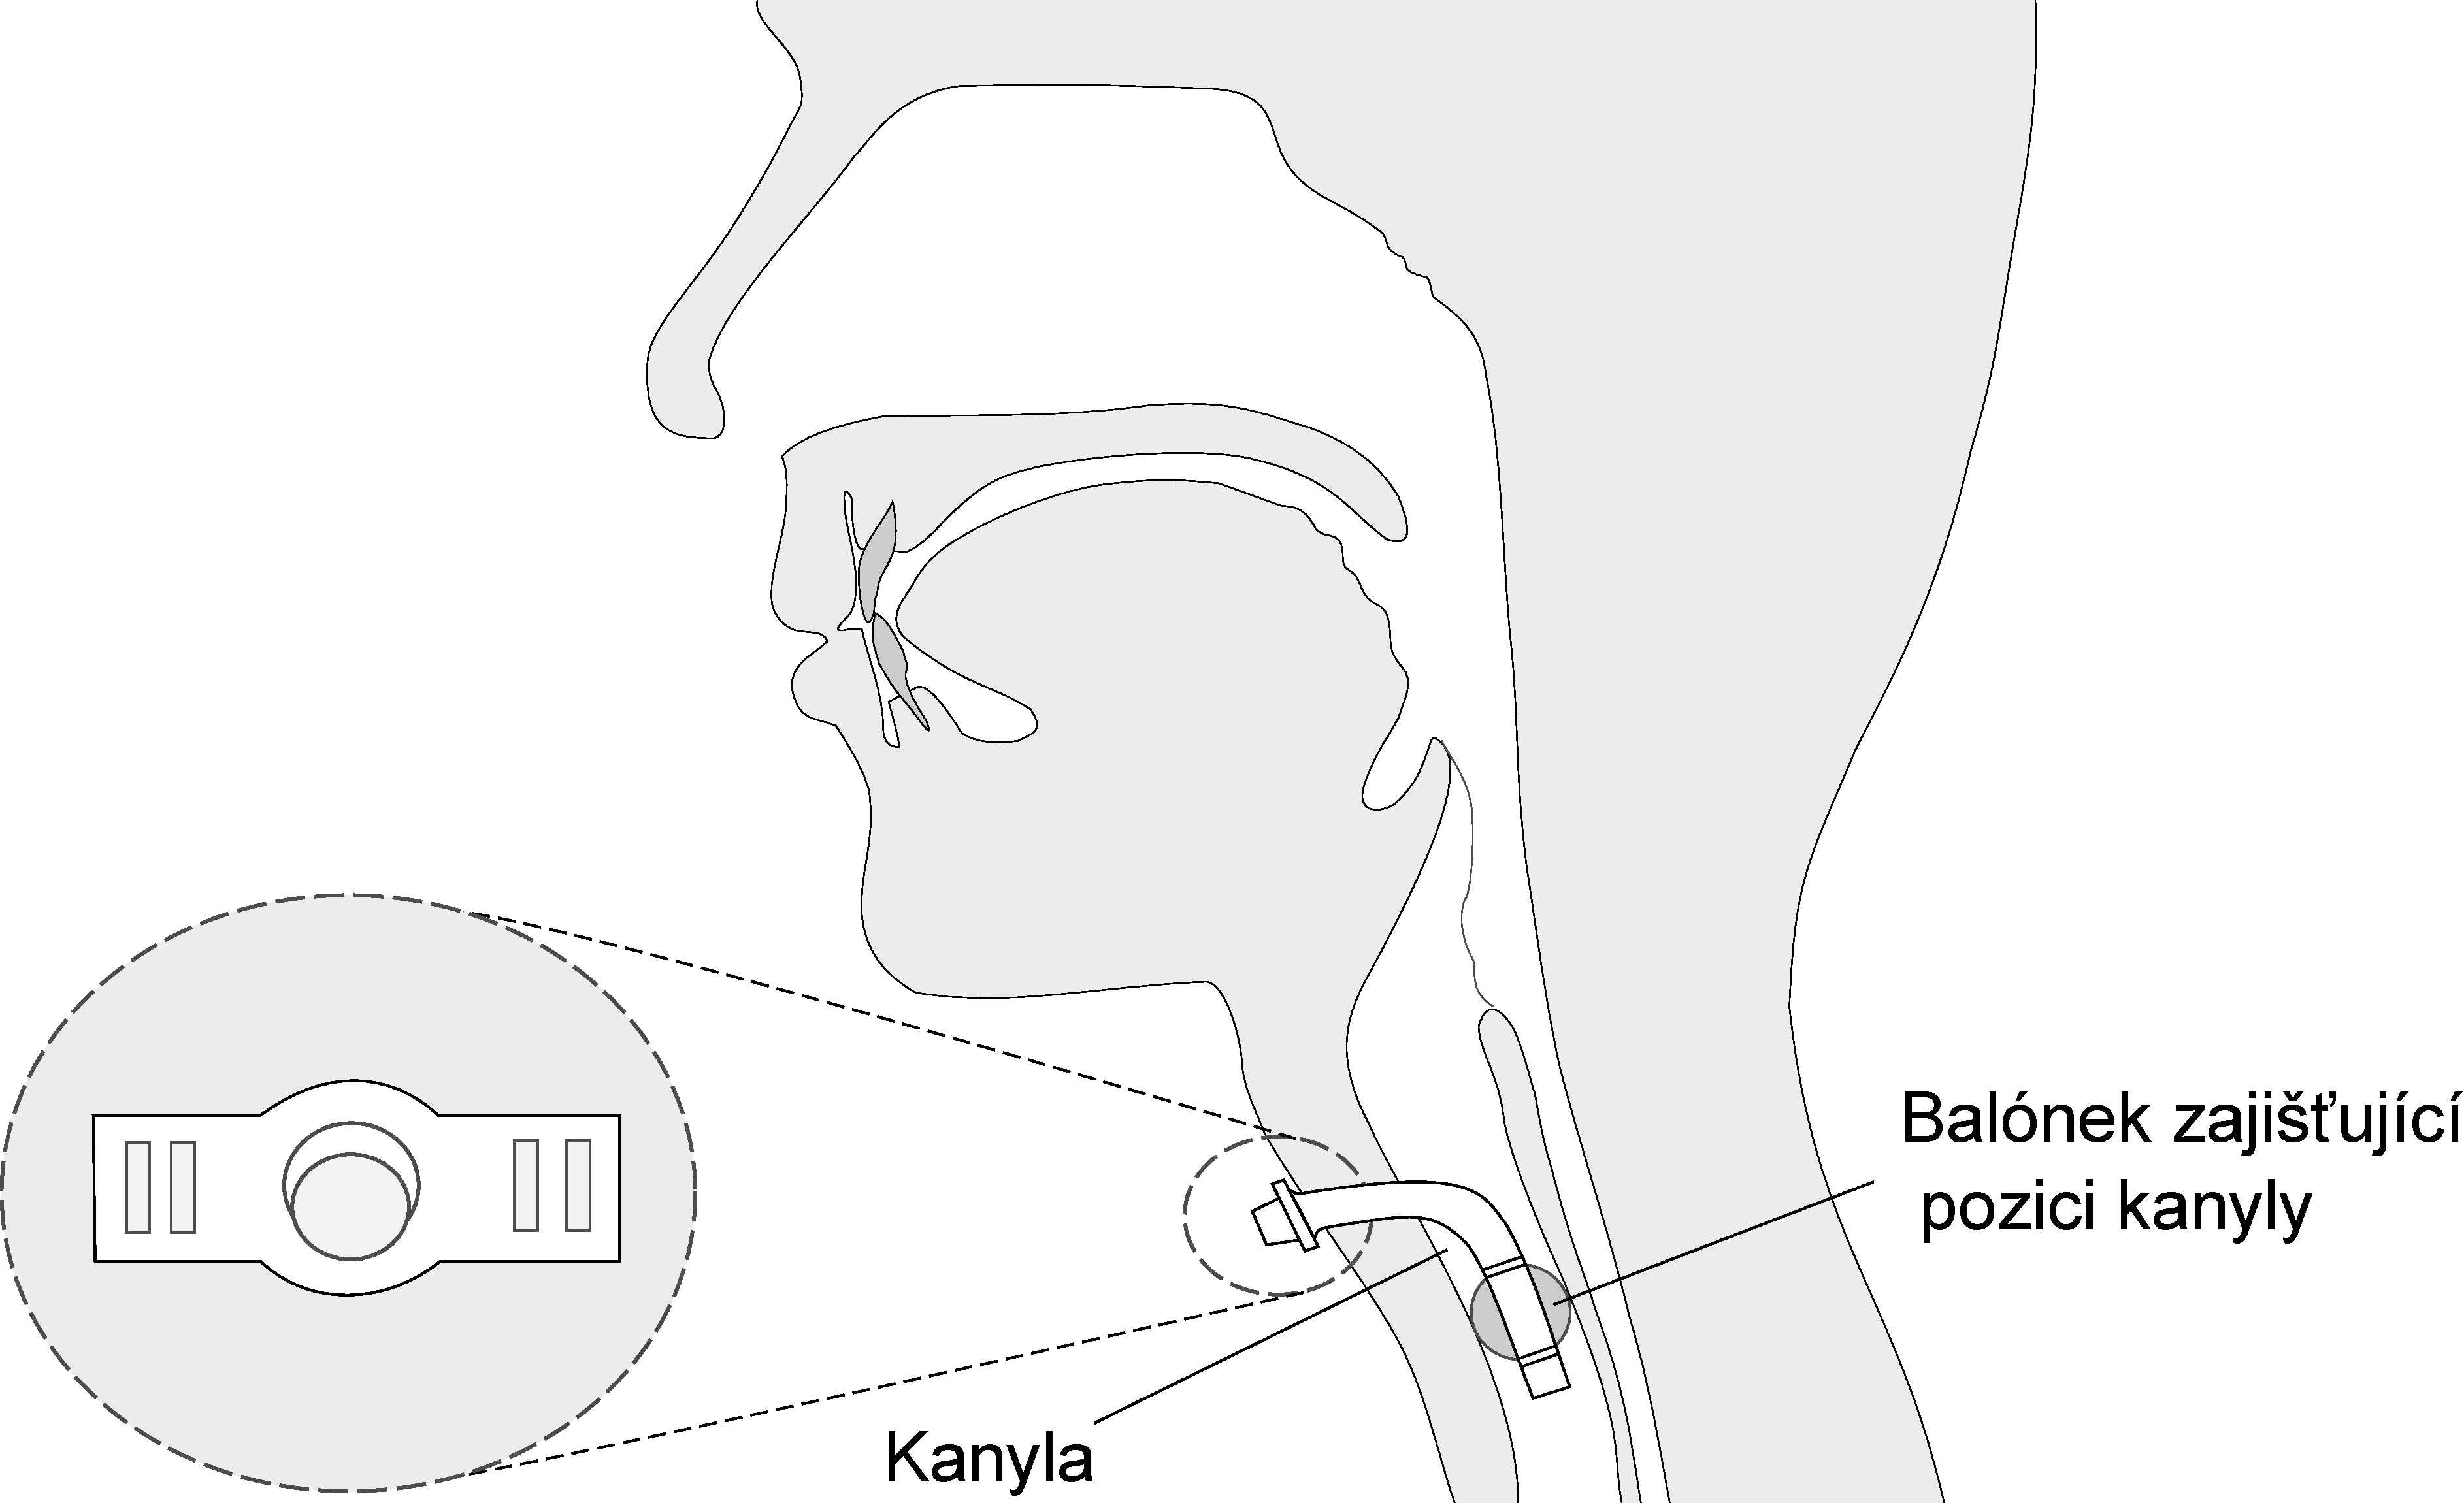
\includegraphics[width=0.9\linewidth]{ch3-cause/figures/tracheostomie}
    \caption[Tracheostomie]{Tracheostomie}
    \label{fig:cause:desease:tracheostomy}
  \end{center}
\end{figure}

Další významnou metodou využívanou k léčbě nádorových onemocnění představuje
\textbf{aktinoterapie} neboli léčba ozařováním. Podstatou postupu je
periodické vystavování buňky ionizujícímu záření. Energie z tohoto záření je
předávána buňce, která je tím poškozována. Tento postup se opírá o předpoklad,
že nádorové buňky jsou náchylnější k poškození. Záření ovšem ovlivňuje i
zdravé buňky, a proto je tato léčba pro organismus velkou zátěží.
Aktinoterapie je možné využít jednak u případů, kdy je cílem terapie úplné
vyléčení, tak i v případech, kdy naprosté odstranění onemocnění není možné. V
druhém případě je metoda využívána k prodloužení a zkvalitnění života
\cite{Slavicek2000}.

Aktinoterapii je možné využít jako hlavní léčebnou metodu (primární
aktinoterapie) nebo i ve spojení s ostatními metodami. V případě primární se k
léčbě využívá pouze ozařování a cílem je úplné odstranění všech defektních
buněk. Z podstaty metody, zejména dopadů léčby na lidský organismus, je
zřejmé, že tímto způsobem je ve většině případů možno léčit pouze malé nádory.

Ve spojení s chirurgickou léčbou rozlišujeme předoperační, pooperační nebo
tzv. sandwich (tj. před a po chirurgickém zákroku) aktinoterapii. Předoperační
ozařování je užíváno v případech, kdy není možné původní nádor vyoperovat.
Cílem je zmenšení tumoru do takové míry, aby jej bylo možné chirurgicky
odstranit. Někdy je předoperační ozařování spojeno s chemoterapií.
U pooperační aktinoterapie je záměrem odstranění potencionálních
mikroskopických zbytků tumoru, které by mohly znovu začít růst.

Velmi často se ve spojení s léčbou rakoviny mluví i o proceduře zvané
\textbf{chemoterapie}. Podstatou je podávání léků zastavujících buněčné
dělení, tzv. cytostatik. Zjednodušeně řečeno se jedná o velmi toxický koktejl
látek sloužící k zahubení buňky tím, že poškodí určitou její část a zastaví
tak proces dělení. Na tuto léčbu jsou citlivé převážně rychle se dělící buňky.
Právě defektní buňky v tumoru mají obvykle určitým způsobem poškozeny opravné
mechanizmy a cytostatiky zasažená rakovinná buňka tak s větší pravděpodobností
zahyne. Samozřejmě nelze u chemoterapie hovořit o přesně zacílené léčbě.
Cytostatika postihují všechny buňky v lidském těle, a proto je možná namístě
srovnání s kobercovým bombardováním. S aplikací cytostatik je tak
spojena celá řada vedlejších rizik. Mezi nejzávažnější patří poškození ledvin
nebo poškození krvetvorby.

% \footnote{Při kobercovém bombardování
% dochází při ničení konkrétního cíle, ke zničení rozlehlé oblasti území. K
% prvnímu použití došlo ve Španělské občanské válce v roce 1937 a k hlavnímu
% rozmachu došlo v průběhu 2. světové války.}

Z výše uvedeného je zřejmé, že postižená osoba má velkou šanci na kompletní
vyléčení. V mnoha případech má však pacient trvalé následky (trvalá ztráta
hlasu) z~důvodu podcenění prvotních příznaků vážného onemocnění.

% subsubsection léčba_nádorového_onemocnění (end)

% subsection rakovina_hrtanu (end)

% %!TEX root = ../thesis.tex
\section{Rehabilitace hlasu po totální laryngektomii}
\label{sec:cause:treatment}

Nesporná výhoda totální laryngektomie neoddiskutovatelně spočívá v likvidaci
primárního nádorového onemocnění. Následky operace však s sebou nesou obrovský
zásah do kvality života pacienta. Okem nejviditelnější změnu představuje
přítomnost tracheostomie a s ní spojený způsob dýchání. Tato skutečnost má
spoustu, na první pohled ne úplně očividných, následků. Postižený člověk
ztrácí přirozené zvlhčování, ohřev a filtraci vdechovaného vzduchu, jež má za
následek vyšší náchylnost k~respiračním onemocněním. Příčina spočívá v
průchodu vzduchu do průdušnice přes tracheostomii a nikoli přes nosní dutiny.

Pro samotného pacienta je však nejspíše nejobtížnější se vypořádat s trvalou
ztrátou vlastního hlasu. Z tohoto důvodu se již samotný autor procedury doktor
Billroth zaobíral otázkou rehabilitace hlasu. Jeho první pokusy s kovovou
tracheostomickou kanylou sice umožňovaly pacientovi hovořit, ale svou
konstrukcí pacienta spíše ohrožovaly na životě \cite{Kramp2009}. Proto se více
uchytila metoda tzv. jícnového hlasu \cite{Sebova-Sedenkova2006}. Ve stejnou
dobu, tedy přibližně začátkem minulého století, se začaly objevovat první
interní a externí hlasové aparáty. V současnosti je rehabilitace hlasu možná
pomocí:

\begin{itemize}
  \item \textbf{foniatrických metod}, mezi které patří jícnový hlas a elektrolarynx,
  \item \textbf{chirurgicko-protetickým způsobem}, který spočívá ve vytvoření kanálku skrze stěnu mezi průdušnicí a jícnem,
  \item \textbf{vytvoření hrtanu podobných struktur chirurgickým způsobem},
  \item \textbf{transplantace hrtanu}.
\end{itemize}

Z uvedeného výčtu se může zdát, že máme k dispozici relativně širokou škálu
možností, jak pacientovi vrátit schopnost vyjadřování pomocí mluvené řeči.
Ovšem je nutné si uvědomit, že je potřeba volit konkrétní metodu podle stavu a
možností pacienta. Jinými slovy, ne každá metoda se hodí pro každého pacienta
a žádná z~metod není univerzální pro všechny pacienty.

\subsection{Foniatrické metody} % (fold)
\label{sub:cause:treatment:foniatric}

Ačkoli odstranění hrtanu vyústí ve ztrátu hlasu, neznamená to, že by byla
úplně eliminována schopnost produkovat řeč. V procesu vytváření hlasu zastává
odstraněný orgán pouze (i když velmi zásadní) roli generátoru zvuku. Zbylé
orgány (hrdelní, nosní a ústní dutina a další) zůstávají nedotčeny a mohou i
nadále plnit svou funkci. Logicky se tak nabízí myšlenka nahradit chybějící
zdroj zvuku jiným. Mezi nejpoužívanější metody patří jícnový hlas a
elektrolarynx.

\subsubsection{Jícnový hlas} % (fold)
\label{ssub:cause:treatment:foniatric:esophageal}

Počátek této metody se datuje do roku 1922, kdy si prof. MUDr. Miloslav Seeman
\cite{seeman1922speech} uvědomil, že funkci štěrbiny mezi hlasivkami (rima
glottidis) přebírá tzv. pseudoglottis, která se vytváří na úrovni horního
jícnového svěrače. Zároveň vypracoval a popsal metodiku vytváření jícnového
hlasu, při které se vzduch neplní do plic, ale do jícnu. Tato metoda se nazývá
\textbf{aspirační}. Princip spočívá v aktivním otevření jícnového svěrače,
nasáváním a vtlačováním vzduchu do jícnu pomocí polykání. Naplněním jícnu
vzduchem si pacient připravuje potřebný vzduch k následné
eruktaci\footnote{eruktace - latinsky název pro proces říhání (popřípadě
krkání), při kterém dochází k úniku plynů pocházejících ze žaludku dutinou
ústní.} vzduchu a produkci řeči. Vlastní jícnový hlas poté vzniká na přechodu
jícnu a hypofaryngu (spodní část hltanu). V této oblasti horního jícnového
zúžení dochází k rozkmitání sliznice a podslizniční vrstvy a produkci zvuku,
který je následně modulován stejně jako v případě přirozené produkce řeči.
Princip tvorby \uv{základního} tónu jícnového hlasu je znázorněn na obr.
\ref{fig:cause:treatment:esophageal}.

\begin{figure}[htb]
  \begin{center}
    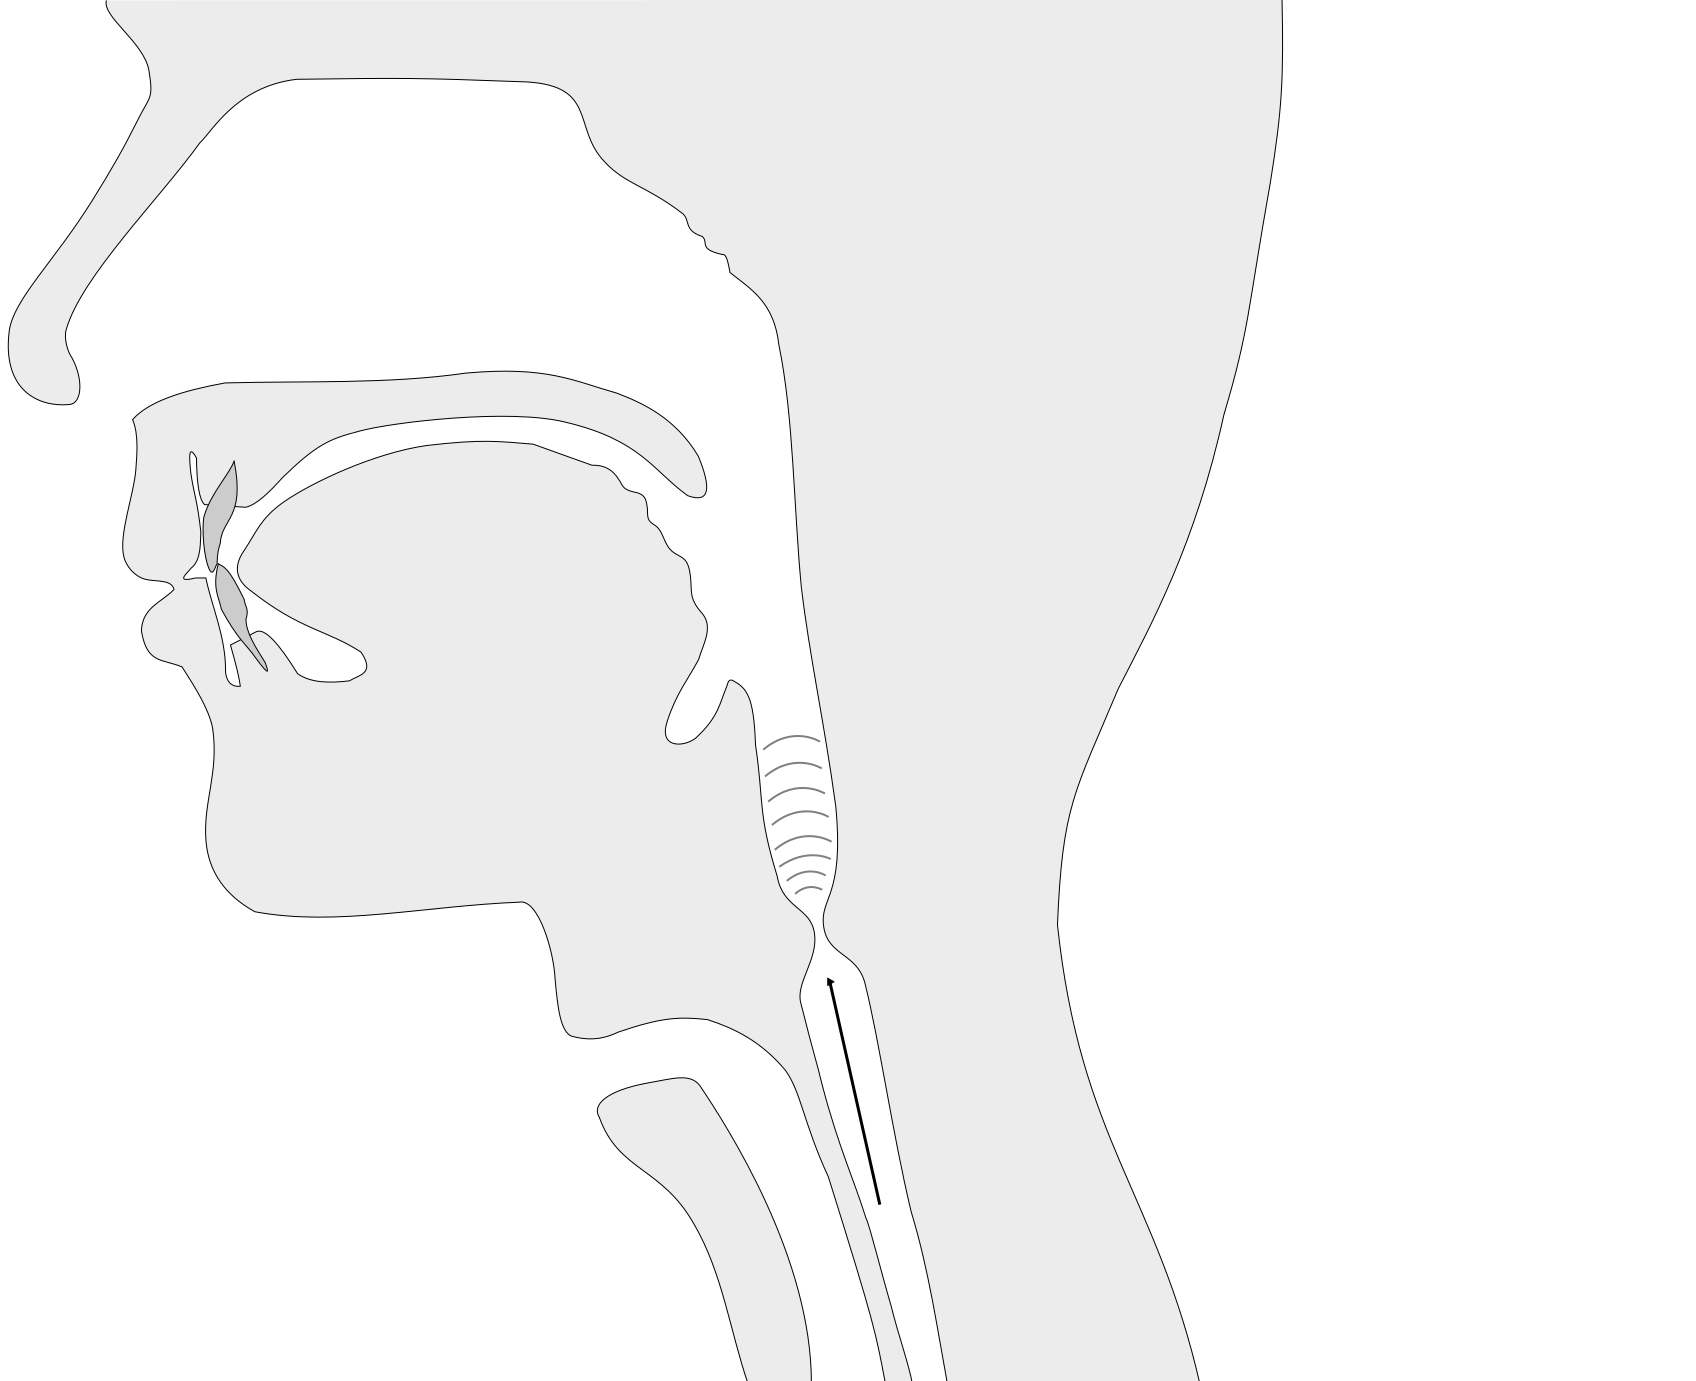
\includegraphics[width=0.6\linewidth]{ch2-cause/figures/esophageal}
    \caption[Princip tvorby jícnového hlasu]{Princip tvorby jícnového hlasu. Průchodem vzduchu přes zúžení vzniká základní tón jícnového hlasu.}
    \label{fig:cause:treatment:esophageal}
  \end{center}
\end{figure}

Kromě aspirační metody je ještě možné se setkat s metodou \textbf{injekční}.
Hlavní rozdíl spočívá v principu plnění vzduchu do jícnu. Při aspirační metodě
se využívá polykání, zatímco v tomto případě je využito kořene jazyka, kterým
je vzduch vtlačován do jícnu. Následný princip produkce hlasu je již shodný s
původní metodou. S tímto principem se můžeme setkat u pacientů, kterým byla
při laryngektomii odstraněna jazylka a aspirační náplň není možná.

Proces učení jícnového hlasu by měl začít co možná nejdříve po operaci. Pokud
je to možné, tak se s výukou začíná ještě za pobytu pacienta na ORL klinice
nebo krátce po propuštění. V první fázi se pacient učí pouze slabiky
sestávající z explosivy a souhlásky. Postupně se však přidávají slabičné
shluky, které sice nedávají smysl, ale pomáhají v osvojení potřebné techniky.
V případě úspěšného zvládnutí se přistupuje k nácviku frází a souvislé řeči.
Potřebnou dobu k nácviku jícnového hlasu nelze přesně určit, protože je
závislá na mnoha faktorech. V literatuře se uvádí, že je potřeba 30 až 50
hodin velmi intenzivního tréninku k osvojení jícnového hlasu.

Míra úspěšnosti nácviku srozumitelného hlasu se uvádí v rozsahu od 14\% do
75\%. Takto obrovský rozsah značí o mnoha faktorech, které mohou ovlivnit
úspěšné osvojení jícnového hlasu. Mezi možné příčiny neúspěchu patří
fyziologické nebo anatomické problémy, psychologické problémy, nebo jednoduše
neadekvátní podpora při řečové terapii \cite{Brown2003}. Velkou roli také
hraje snaha a odhodlání samotného pacienta.

Nepopíratelnou výhodou této techniky rehabilitace je nezávislost pacienta na
lékaři po úspěšném osvojení jícnového hlasu a permanentní oddělení dýchacích a
polykacích cest bez rizika vniknutí potravy do dýchacích cest. Mezi nesporné
výhody také patří volné ruce při vytváření řeči. Za nevýhody se obecně
považuje srozumitelnost produkovaného hlasu. Je to způsobeno jednak
\uv{břišním} zabarvením, které je už z podstaty metody přítomné, a dále také
nízkou intenzitou a krátkou výdrží při tvorbě tónu. Za negativum se dá také
považovat množství pacientem vynaloženého úsilí potřebného k osvojení
techniky. Velmi často se také mluvčí ostýchají jícnový hlas používat, protože
mají pocit, že je společensky nevhodné dorozumívat se formou blízkou říhání. Z
tohoto důvodu se odhaduje, že v běžném životě využívá jícnový hlas pouze 20 až
30\% pacientů, kteří se začali tuto techniku učit \cite{Hradecka2007}.

% subsubsection jícnový_hlas (end)

\subsubsection{Elektrolarynx} % (fold)
\label{ssub:cause:treatment:foniatric:elektrolarynx}

Rehabilitace hlasu pomocí elektrolarynxu se řadí mezi tzv. elektromechanické
metody. Princip spočívá v přikládání zařízení, které obsahuje generátor zvuku
nazývaný elektrolarynx. Přiložením do oblasti spodiny úst a aktivací zařízení
se generovaný zvuk a vibrace přenášejí do dutiny ústní a dalších přilehlých
artikulačních orgánů. Následnou artikulací je pacient schopen hovořit.
Znázorněno na obr. \ref{fig:cause:treatment:electrolarynx}.

\begin{figure}[htb]
  \begin{center}
    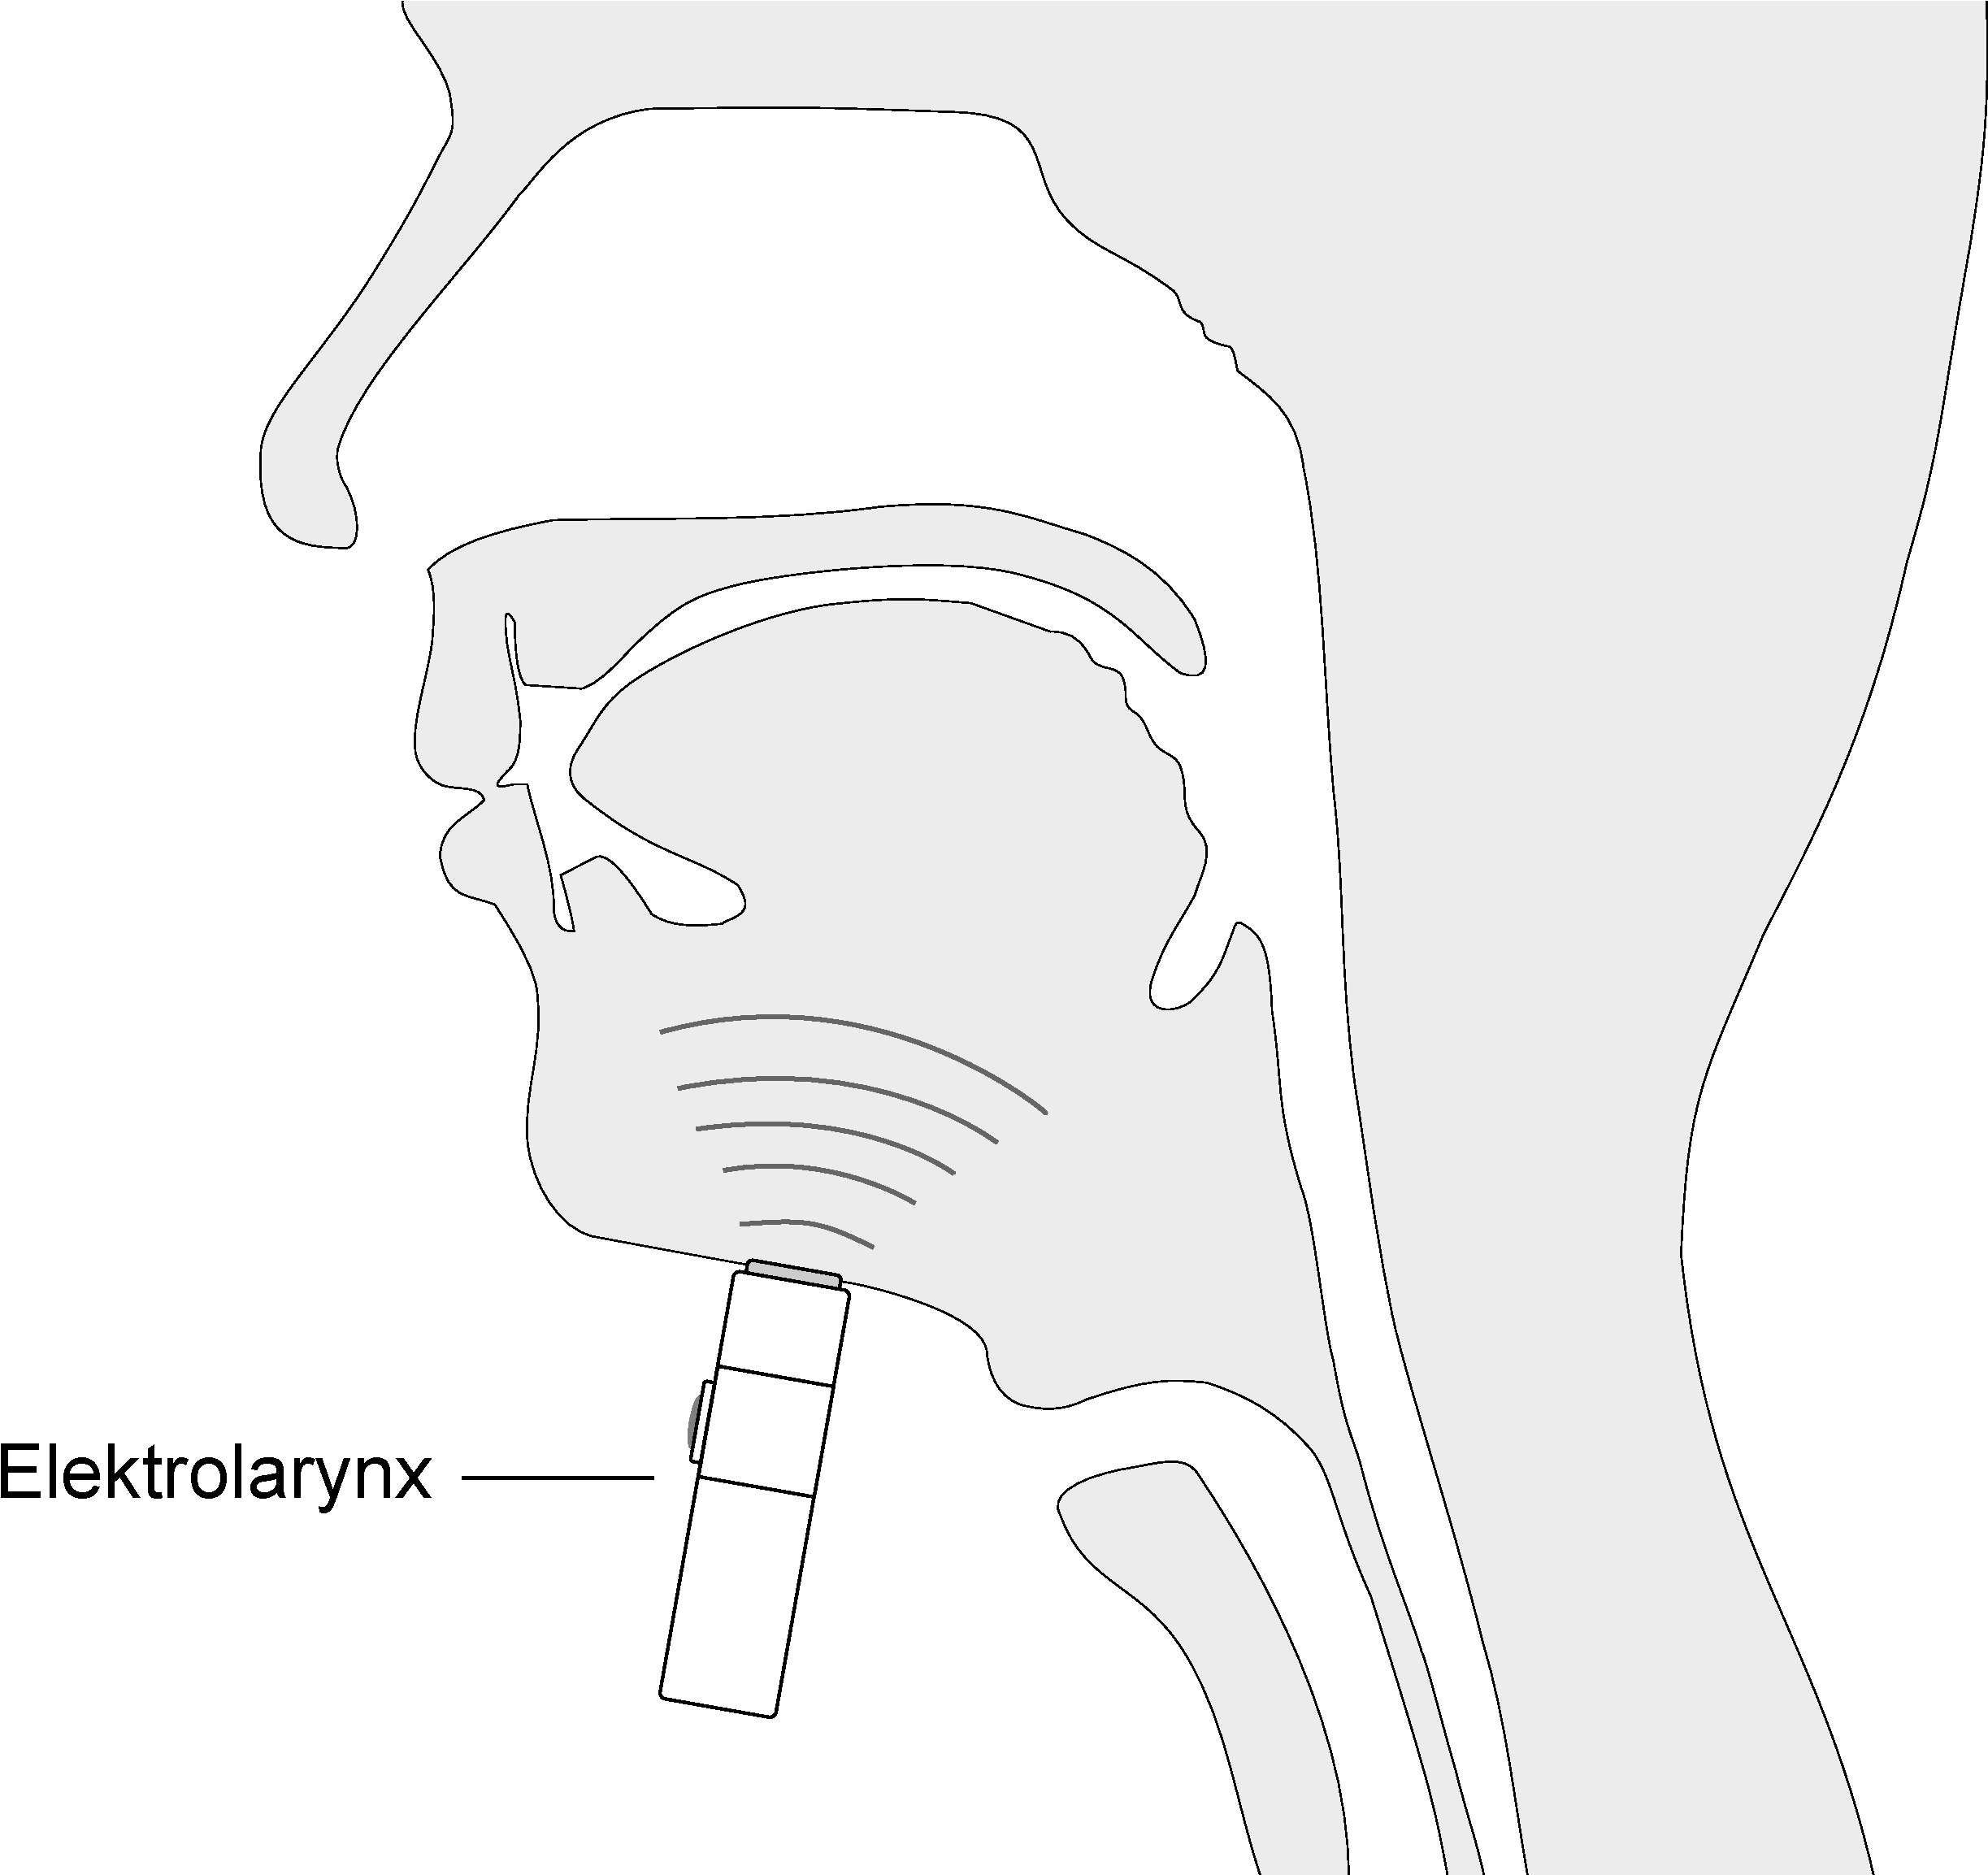
\includegraphics[width=0.6\linewidth]{ch2-cause/figures/electrolarynx}
    \caption[Princip rehabilitace hlasu pomocí elektrolarynxu]{Princip rehabilitace hlasu pomocí elektrolarynxu.}
    \label{fig:cause:treatment:electrolarynx}
  \end{center}
\end{figure}

% TODO: ELEKTROLARYNX pasaze o monotonosti reci poradne promyslet

Takto generovaná řeč se vyznačuje několika charakteristickými rysy. V první
řadě řeč budí velmi mechanický dojem. Důvodem je samozřejmě samotný
elektrolarynx, jelikož se jedná o elektromechanický generátor zvuku s
konstantním buzením, je také základní frekvence produkovaného hlasu více či
méně konstantní. Řečník tak má velmi omezené možnosti, jak řeč emotivně
zabarvovat. V průběhu času se objevily snahy průběžně měnit frekvenci zařízení
a tím ovlivňovat základní frekvenci produkované řeči \cite{Kikuchi2004,
Uemi1994, Goldstein2004}. Hlavním problém všech těchto zařízení je docílit
změnu fundamentální frekvence na základě toho, co chce řečník říci. V současné
době existují pouze experimentální zařízení, která umožňují ve velmi omezené
míře změnu frekvence \cite{Liu2007}. Další charakteristický rys představuje
nižší srozumitelnost řeči, která se ještě snižuje s~rostoucím okolním hlukem.
Velmi často se stává, že posluchač, který se s takto produkovanou řečí setkává
poprvé, není schopen plně porozumět. Se srozumitelností souvisí i další
charakteristický rys, kterým je přítomnost zvukového podkresu produkovaného
samotným přístrojem.

Za hlavní výhodu elektrolarynxu se považuje rychlost osvojení schopnosti
produkovat řeč. Zároveň je tato metoda vhodná pro téměř všechny pacienty
postižené ztrátou hlasu způsobenou léčbou karcinomu hrtanu. Z tohoto důvodu se
hojně užívá u pacientů, kteří si neosvojili jícnový hlas nebo u nich není
možné využití ostatních chirurgických metod.
Za nevýhody se obecně pokládá kvalita produkované řeči, tedy monotonní a
mechanicky znějící hlas. Dále potom zaměstnání jedné ruky držením nebo
spouštěním zařízení.

Samostatnou kapitolou může být psychologický dopad na pacienta. Stejně jako
u~jícnového hlasu se řeč produkovaná promocí elektrolarynxu jeví odlišně od
řeči přirozené. Navíc se ještě přidává potřeba využití nějakého zařízení.
Člověk proto v~mnoha případech cítí ostych a bojí se na veřejnosti mluvit.

% subsubsection elektrolarynx (end)

% subsection subsection_name (end)

\subsection{Chirurgicko-protetická metoda} % (fold)
\label{sub:cause:treatment:tracheo}

Další možnost rehabilitace hlasu představuje tracheoezofageální (zkr. TE) protéza.
První zmínka o vytvoření fistule\footnote{fistule (česky píštěl) je abnormální
otvor mezi dvěma dutými orgány, nebo mezi dutým orgánem a kůží.} mezi
průdušnicí a jícnem pochází z roku 1932. V~tomto roce doktor Guttman poprvé
vytvořil tracheoezofageání shunt\footnote{shunt - kanál, kterým je tekutina
odkloněna z přirozené dráhy. Tento kanál může být vytvořen chirurgicky nebo
pomocí syntetické trubice.} (\uv{umělá píštěl}). Hlavní myšlenka spočívá ve
vytvoření cesty prostřednictvím píštěle, pomocí které u tracheostomovaného
člověka může proudit vzduch z plic do úst. Za normálních okolností vzduch
proudí skrze tracheostomii a do úst se tak nedostane. Zacpe-li si pacient
stomu, může proud vzduchu proudit skrze píštěl do úst. Vzduch procházející
přes fistuli naráží do stěn jícnu a je rozvibrován. Tyto vibrace jsou následně
modulovány pomocí artikulačních ústrojí a tak vzniká řeč.
Tento ojedinělý zákrok otevřel cestu k chirurgické hlasové rehabilitaci.
Vzniklo několik operačních metod, které se navzájem lišili víceméně jen
umístěním fistule \cite{Kramp2009}.

Hlavní snahou chirurgů bylo vytvoření bezpečné, správně nasměrované píštěle
umožňující tvorbu hlasu. Bohužel v mnoha případech byly tyto zákroky spojené
s~vážnými komplikacemi (infekce, zápaly či těžká krvácení). Důležitým
problémem, se kterým se jednotlivý tvůrci museli vypořádat, byla stálost
vytvořeného otvoru tak, aby jím neprotékaly tekutiny špatným směrem a
nedocházelo k zatékání do dýchacích cest a orgánů. Jelikož se jednalo o velmi
náročné techniky, a bylo s nimi spojeno velké množství rizik, došlo v
80.letech 20.století k opadnutí snah tyto metody aplikovat.

Svou renesanci zažily s vložením jednocestného ventilu, který umožňoval pouze
jednosměrný průchod tekutin skrze píštěl, jak je ilustrováno na obr.
\ref{fig:cause:treatment:shunt}. První komerčně dostupná protéza se objevila
v~80.letech 20.století v USA. Na obr. \ref{fig:cause:treatment:prosthesis} jsou
zobrazeny příklady různých typů protéz. Na používané protézy jsou kladené
přísné nároky a musí vyhovovat určitým požadavkům. Předně se musí vyrábět
z~biokompatibilního materiálu, který odolává biodegradaci. Tím je zaručena
dlouhodobá trvanlivost a správná funkce. Potřebný tlak k otevření
faryngoezofageálního segmentu by měl být co nejnižší, aby bylo možné vytvářet
plynulou řeč. První vyráběné protézy měly tento tlak příliš vysoký a omezovaly
tak množinu potencionálních pacientů. Nejmodernější protézy se již vyznačují
velmi nízkým otevíracím fonačním tlakem. V~neposlední řadě by měla být protéza
samofixační a snadno vyměnitelná.

\begin{figure}[htb]
  \begin{center}
    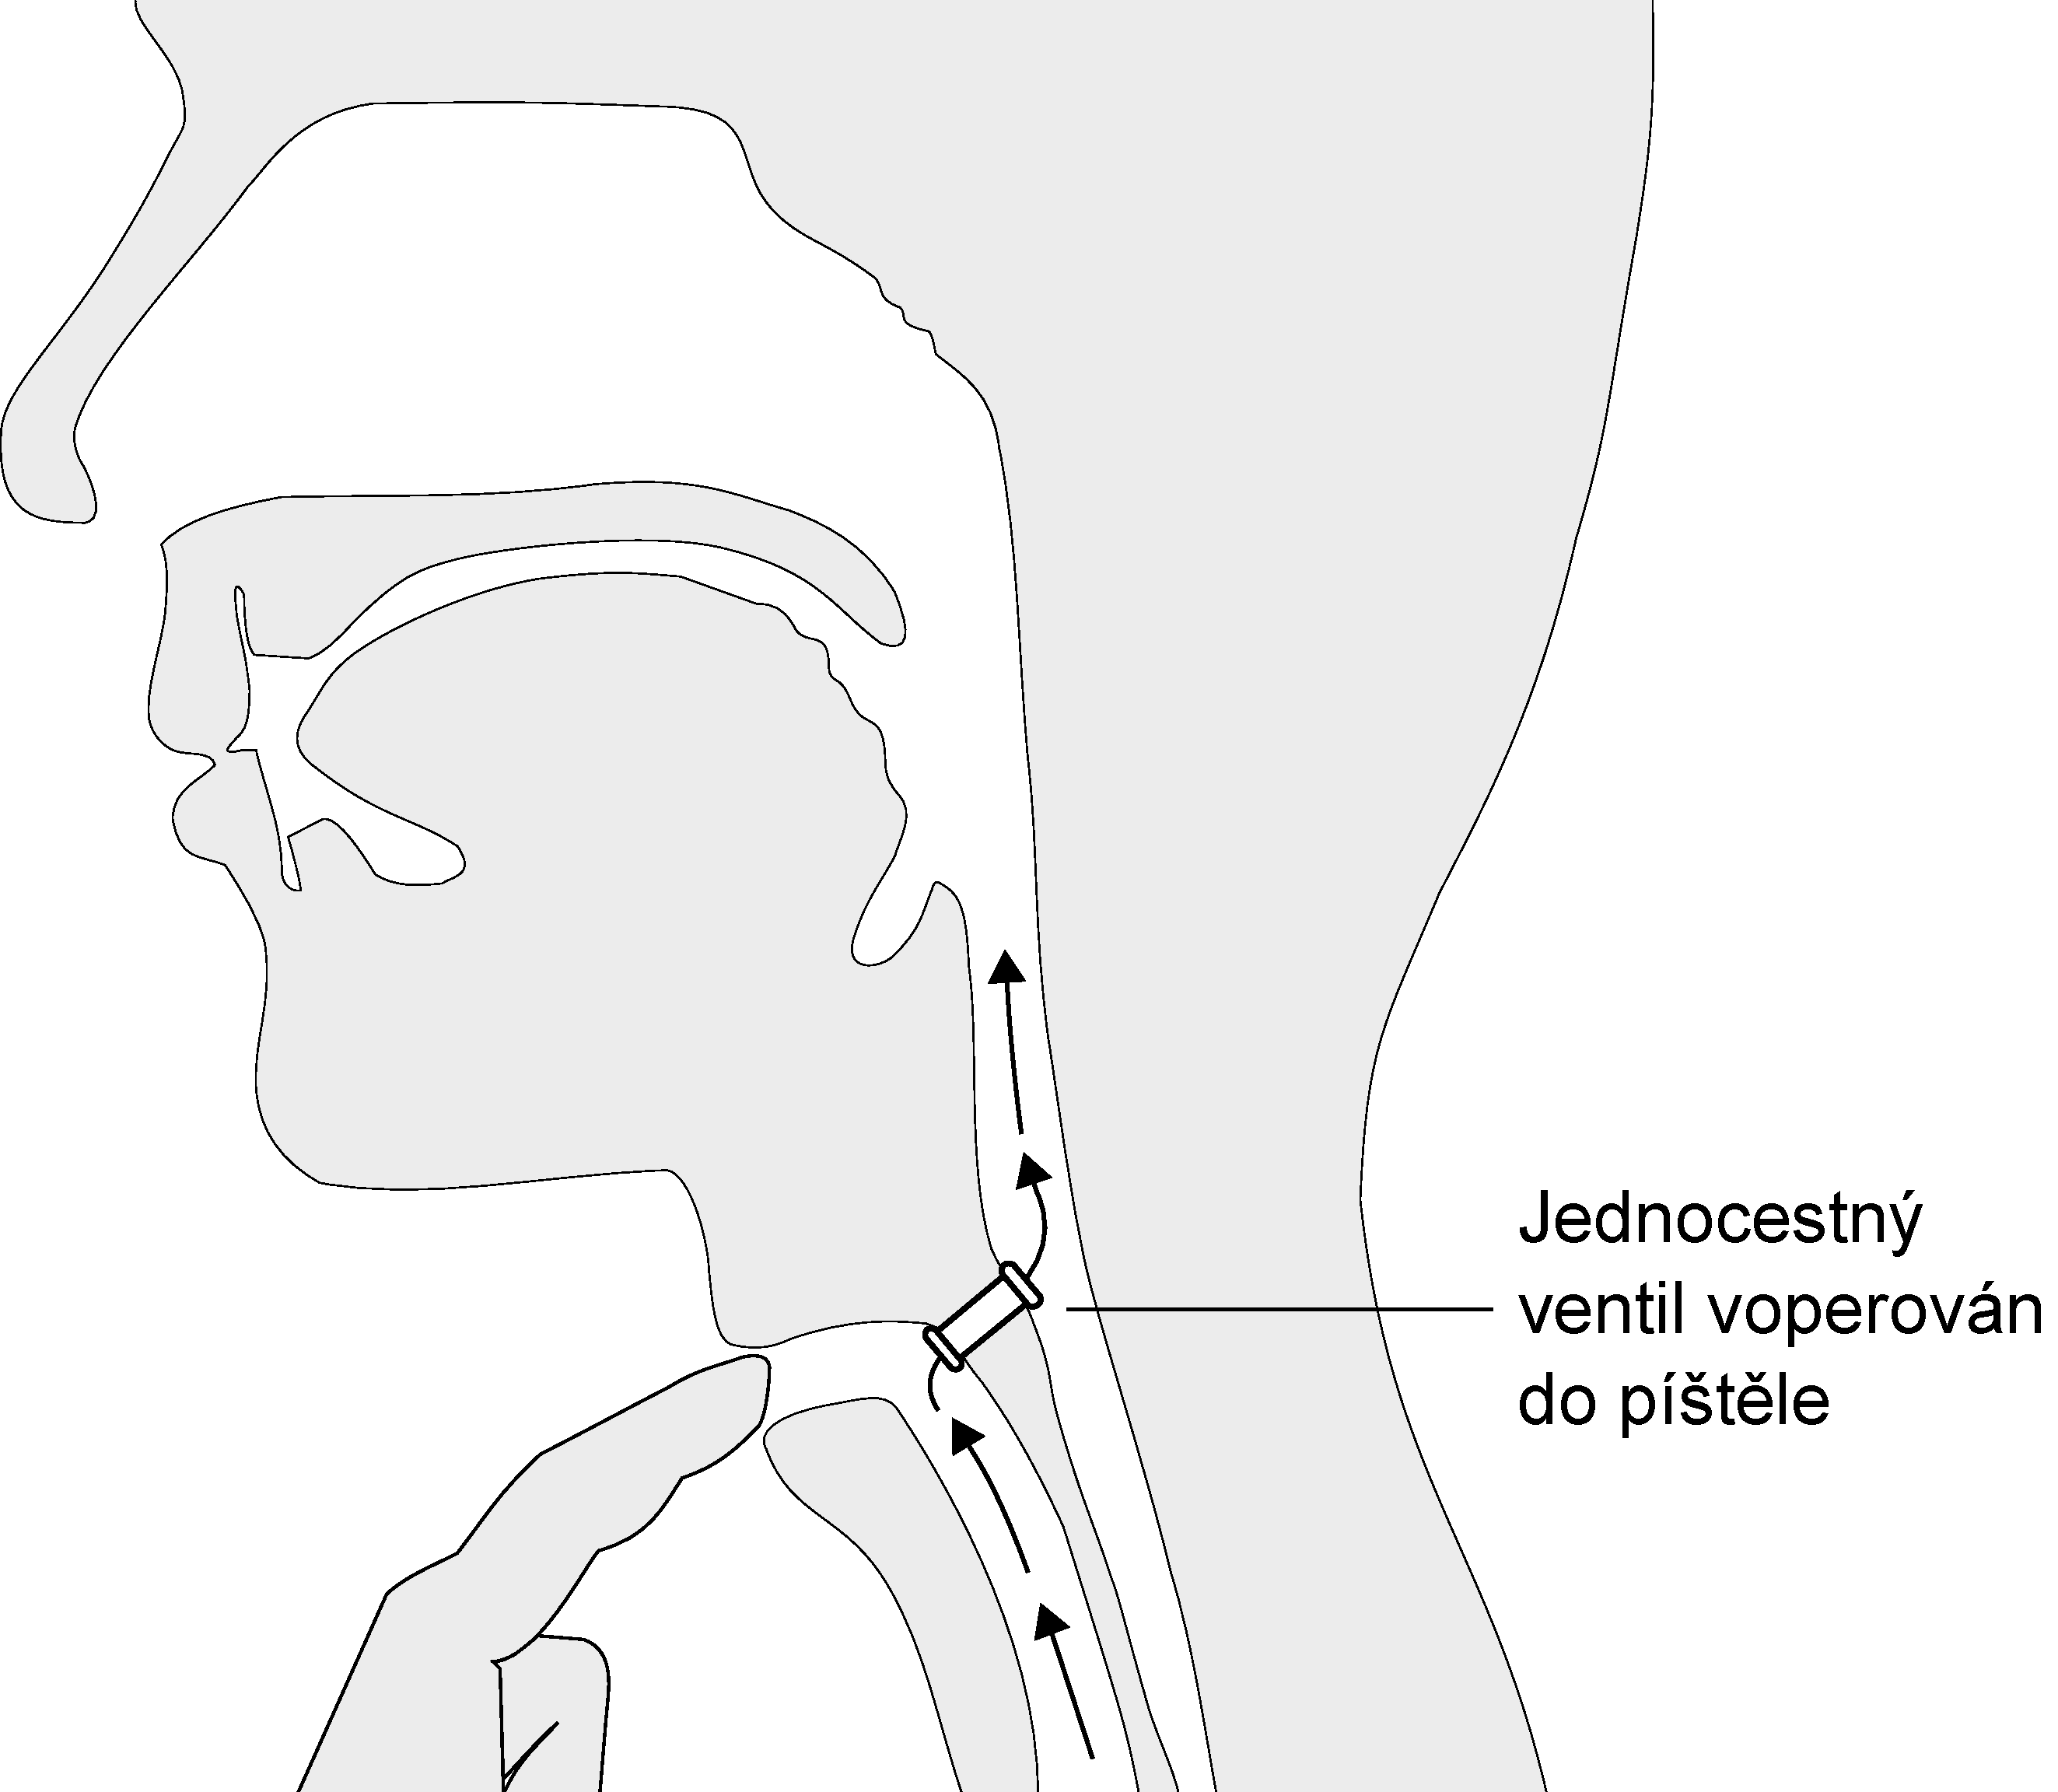
\includegraphics[width=0.6\linewidth]{ch2-cause/figures/te-shunt}
    \caption[Průchod vzduchu tracheoezofageální protézou]{Průchod vzduchu tracheoezofageální protézou.}
    \label{fig:cause:treatment:shunt}
  \end{center}
\end{figure}

\begin{figure}[htb]
  \begin{center}
    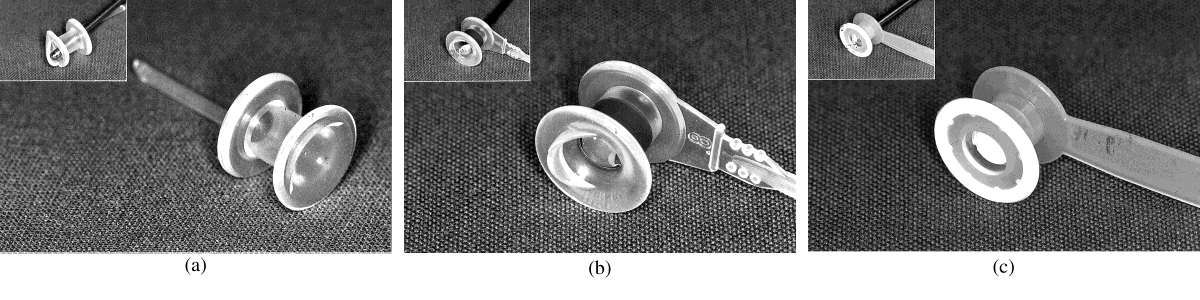
\includegraphics[width=0.9\linewidth]{ch2-cause/figures/te-protezy}
    \caption[Ilustrace používaných TE protéz]{Ilustrace používaných TE protéz (a) Gronigenova nízkotlaká protéza, (b) Provox2 a (c) Blom-Singer protéza.}
    \label{fig:cause:treatment:prosthesis}
  \end{center}
\end{figure}

V praxi se používá několik druhů protéz. Hlavním rozdílem mezi nimi však je
zda se pacient přímo účastní výměny ventilu, jehož fundamentální funkcí je
vytvoření průchodu pro vzduch proudící z průdušnice do jícnu. U protéz, které
jsou vyměňovány operačně, se doba používání pohybuje od 3 do 6 měsíců. Tento
interval velmi významně ovlivňuje tvorba biofilmu na povrchu náhrady. K tvorbě
dochází následkem přímého kontaktu protézy s tělními tekutinami a potravou.
Rychlost tvorby biofilmu ovlivňuje tvar a materiál, ze kterého je náhrada
vytvořena \cite{Leunisse2001}. U typů, které si nositel může měnit sám, se
předpokládá, že budou čištěny nebo měněny přibližně jednou za dva týdny.

Samotný zákrok zavedení protézy je možné provést zároveň s výkonem totální
laryngektomie (tzv. primární zavedení hlasové protézy) nebo až po zotavení
pacienta z~náročné léčby nádorového onemocnění (tzv. sekundární zavedení).
Primární zavedení umožňuje začít s hlasovou rehabilitací krátce po odstranění
hrtanu. Zároveň pacient nemusí v krátké době podstupovat druhou operaci, při
které by se vkládal jednocestný ventil do vytvořené fistule.

V praxi se ukázalo, že úspěšnost rehabilitace je více než 80\%
\cite{Slavicek2002}. Důležitým faktorem, stejně jako u jícnového hlasu, je
funkčnost faryngoezofageálního segmentu. Dále také otvírací tlak horního
jícnového svěrače. Hlas tvořený protézou se vyznačuje vysokou kvalitou, dobrou
srozumitelností, individuálním zabarvením a relativně dlouhou fonační dobou
dosahující průměrně 20 sekund \cite{Saito2003}. Oproti jícnovému hlasu není potřeba
tak intenzivní edukace pacienta k plnému osvojení hlasu. V současnosti se
jedná o nejpoužívanější metodu rehabilitace hlasu.

% TODO: Vyhody nevyhody metody - film tvorici se na proteze
% TODO: Kriteria na pacienta


% subsection chirurgicko_protetická_metoda (end)

\subsection{Hrtanu podobné struktury} % (fold)
\label{sub:cause:tratment:structure}

S rozvojem mikrovaskulárních\footnote{mikrovaskulární - část oběhového systému
složeného z nejmenších cév, jako jsou kapiláry, žilky aj.} transplantátů se
začaly objevovat postupy, které umožňovaly rehabilitovat hlas pouze pomocí
chirurgického zákroku. Tyto techniky umožňují permanentní spojení hypofaryngu
s tracheou pomocí vlastní tkáně pacienta.

První takovouto  metodu představil v roce 1984 doktor Ehrenberger
\cite{Kramp2009}, který popsal tzv. \uv{\textbf{řečový sifón}} (angl. \textbf{speech
siphon}). Tento sifón je vytvořen z části tenkého střeva zvané lačník
(jejunum). Spojení mezi hrtanem a hltanem je dvakrát esovitě zahnuto tak, aby
bylo minimalizováno riziko sekundární aspirace. Schéma \uv{řečového sifónu}
podle Ehrenberga je znázorněno na obr. \ref{fig:cause:treatment:microvascular}
A. Již na první pohled je zřejmé, že se jedná o velmi náročný chirurgický
zákrok. První články publikované autorským kolektivem prezentovaly velmi dobré
funkční výsledky metody. Podle \cite {Sebova-Sedenkova2006} bylo doposud
operováno přibližně 60 pacientů.

V roce 1990 byla popsána laryngoplastika podle Hagena. V tomto případě se
vytváří tzv. \textbf{neolarynx}, k jehož vytvoření se používá štěp z
předloktí. Vnitřek neolaryngu je kryt kůží. Neoglottis je vyztužen chrupavkou
a překrývá vchod do neolaryngu tak, aby nedocházelo k sekundární aspiraci.
Laryngoplastika podle Hagena je znázorněna na obr.
\ref{fig:cause:treatment:microvascular} B. Doposud bylo operováno přibližně 300
pacientů \cite{Sebova-Sedenkova2006}.

\begin{figure}[htb]
  \begin{center}
    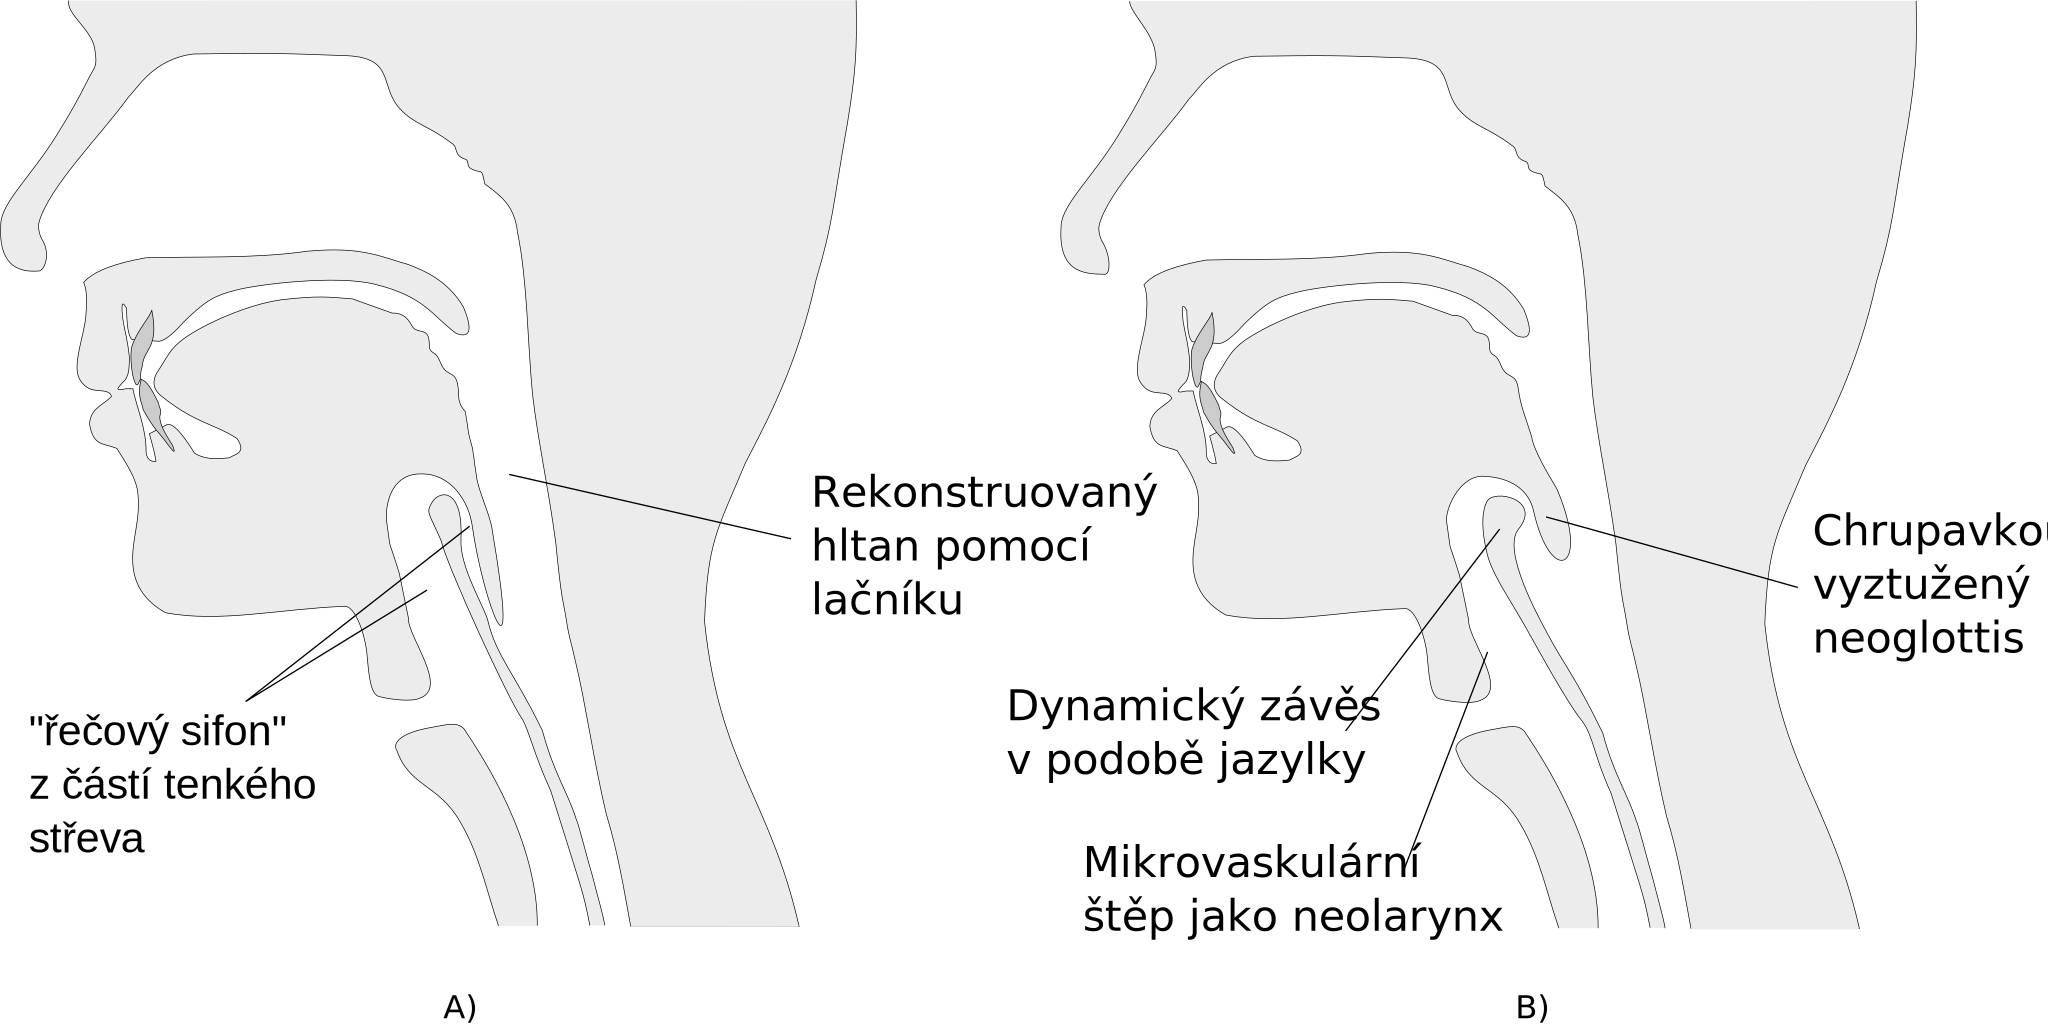
\includegraphics[width=0.9\linewidth]{ch2-cause/figures/microvascular}
    \caption[Schéma \uv{řečového sifónu} a laryngoplastiky]{A) Schéma \uv{řečového sifónu} tak jak jej představil Ehrenberg. B) Laryngoplastika podle Hagena}
    \label{fig:cause:treatment:microvascular}
  \end{center}
\end{figure}

Bohužel v současné době tyto metody nenacházejí širší uplatnění. Především je
to způsobeno chirurgickou náročností samotných metod, kvůli které se velmi
těžko prosazují na dalších pracovištích. Dalším aspektem, který limituje tyto
metody, je vliv na samotného pacienta. Metody předpokládají další chirurgický
zákrok vykonaný po totální laryngektomii. Tento zákrok představuje další zátěž
pro pacienta nemluvě o~možných komplikacích. I přes nedostatky těchto metod je
pochopitelná snaha lékařů o intenzivní výzkum v této oblasti. Při úspěšné
léčbě je pacient schopen produkovat hlas velmi dobré kvality a ve většině
případů nepotřebuje žádnou péči ze strany lékařů ORL.

% subsection hrtanu_podobné_struktury (end)

\subsection{Transplantace hrtanu} % (fold)
\label{sub:cause:treatment:transplantation}

Nejkomplexnější možnost rehabilitace hlasu představuje transplantace hrtanu.
V~tomto případě pacient obdrží implantovaný hrtan od dárce. Pokud je
transplantace úspěšná, přebírá transplantovaný orgán plně funkci původního
orgánu a velmi významně zvyšuje šance pacienta na plné zotavení bez trvalých
následků.

První informace spojené s výzkumem možností provedení transplantace hrtanu se
objevují již v 60. letech 20. století\footnote{Vůbec první úspěšná transplantace
orgánu (ledvin) se uskutečnila v roce 1954.}. Přesto byla první totální
hrtanová transplantace provedena až profesorem Marshallem Stromem v roce 1998
\cite{Narula2011} a do dnešních dnů byly provedeny pouze 2 kompletní
transplantace.

Prvním pacientem, který podstoupil transplantaci, byl čtyřicetiletý muž z USA.
K~laryngektomii v jeho případě vedla motocyklová nehoda, při které si pacient
rozdrtil hrtan. K incidentu došlo 20 let před transplantací. Před zákrokem
používal k~produkci řeči elektrolarynx. Dárcem orgánu byl taktéž čtyřicetiletý
muž, který zemřel na mozkové aneurysma. Úspěch transplantace se na příjemci
projevil již třetí den po operaci, kdy poprvé po 20 letech promluvil (vyslovil
anglické slovo \uv{hello}). Přibližně po 36 měsících od transplantace byl
produkovaný hlas srovnatelný s hlasem zdravého člověka. Podle vlastních slov
pacienta se po operaci jeho kvalita života \uv{nesmírně} zlepšila.
\cite{Strome2001} Doposud poslední úspěšně vykonaná transplantace byla
zaznamenána v~říjnu 2010.

Mezi hlavní důvody takto malého počtu zákroků patří množství pacientů vhodných
pro tuto proceduru. Jelikož se jedná o transplantaci dárcovského orgánu je
nutné použití imunosupresiv, tedy medikamentů zabraňující odmítnutí orgánu.
Imunosupresiva jsou však v současné době nepoužitelná u lidí trpících
rakovinou hrtanu z důvodu velmi vysokého rizika rozšíření rakoviny
\cite{Narula2011}. Další problém představuje náročnost samotného zákroku.
Předně je potřeba provést reinervaci a obnovení krevního oběhu v implantovaném
orgánu. U první provedené transplantace se nepodařilo dosáhnout kompletní
reinervace. Výsledkem tak byl velmi kvalitní generovaný hlas, ale zároveň
nebylo možné pomocí hrtanu zabezpečit bezproblémové dýchání a bylo proto nutné
ponechat tracheostomii.

Poslední výzkum v oblasti imunosuprese však naznačuje, že by v dohledné době
mohlo dojít k pokroku a umožnit transplantaci hrtanu i u lidí trpících
rozsáhlou rakovinou v oblasti krku \cite{Narula2011}. Prozatím je však tato
metoda vhodná pro pacienty netrpící rakovinou, případně ty, u kterých
převažovaly benigní nádory a již 5 let nedošlo k recidivě.

% subsection transplantace_hrtanu (end)

\subsection{Shrnutí} % (fold) \label{sub:treatment:summary}

% NOTE: Neni lepsi pouzit dusledky misto nasledky 3

Rehabilitaci pacientů, kteří prodělali chirurgické odstranění hrtanu, je ve
vyspělých zemích věnována značná pozornost, jelikož následky této operace,
oproti jiným druhům léčby, velmi významně ovlivňují kvalitu života pacientů. V
první řadě se léčený musí vyrovnat se ztrátou hlasu. Tato situace je již sama
o sobě velmi náročnou psychickou zkouškou. Ztráta hlasu je však pouze jedním z
vícero problémů, se kterými je potřeba se vypořádat. Mezi další patří možná
ztráta čichu či vyšší náchylnost k respiračním onemocněním. Neméně významnou
roli sehrává i fyzická odlišnost a z~toho pramenící psychická zátěž pacienta
po absolvované léčbě.

 V současnosti
nejpoužívanějšími metodami rehabilitace hlasu jsou \textbf{tracheoezofageální
píštěl} (popsáno v části \ref{sub:cause:treatment:tracheo}), \textbf{jícnový
hlas} (\ref{ssub:cause:treatment:foniatric:esophageal}) a použití
\textbf{elektrolarynxu} (\ref{ssub:cause:treatment:foniatric:elektrolarynx}).
Existují samozřejmě i další a přehled v současnosti používaných je uveden
v~tab. \ref{tab:treatment:summary}.

\newcolumntype{b}{X}
\newcolumntype{s}{>{\hsize=.5\hsize}X}

\begin{table}[ht]
  \centering
  \begin{tabularx}{1.0\textwidth}{L{1.2} L{0.6} L{1.1} L{1.1}}
    & \textbf{Kvalita} & \textbf{Výhody} & \textbf{Nevýhody} \\
    \toprule \\ [-1.75ex]

    \textbf{Tracheoezofageální píštěl} & Vysoká & Vysoká míra osvojení, dlouhá fonační doba & Zanášení píštěle a s ním spojené čištění, případně dodatečná lékařská péče \\
    \midrule \\ [-1.75ex]

    \textbf{Jícnový hlas} & Dobrá & Volné ruce při mluvení, není potřeba dodatečné lékařské péče & Velmi náročná metoda k naučení, nepřirozený hlas \\
    \midrule \\ [-1.75ex]

    \textbf{Elektrolarynx} & Nízká & Snadné k naučení & Monotonní až robotický hlas, nutné nosit externí elektrické zařízení \\
    \midrule \\ [-1.75ex]

    \textbf{Hrtanu podobné struktury} & Vysoká & Nezávislost pacienta na pravidelné lékařské péči & Velmi náročná chirurgická procedura, která pacienta vystavuje dalším možným rizikům  \\
    \midrule \\ [-1.75ex]

    \textbf{Transplantace hrtanu} & Velmi vysoká & Transplantovaný hrtan přejímá funkci odstraněného orgánu & Velmi náročná chirurgická procedura, která je vhodná jen pro malé procento pacientů \\
  \end{tabularx}

  \caption{Přehled dostupných metod rehabilitace hlasu \label{tab:treatment:summary}}
\end{table}

Většina pacientů je tedy rehabilitována pomocí tracheoezofageálního píštěle,
který principiálně vychází z jícnového hlasu, jehož negativa se snaží
eliminovat. O úspěchu rehabilitace, stejně jako u jícnového hlasu, tak
především rozhodují vlastnosti faryngoezofageálního segmentu. Pokud pacient
není schopen si osvojit jícnový hlas, případně nemá voperován píštěl, je
použit elektrolarynx. Bohužel tyto metody neřeší další problémy spojené s
odstraněním hrtanu, a proto se lékaři stále snaží zdokonalovat rehabilitační
metody. Za nejkomplexnější se dá považovat úplná transplantace hrtanu, která
řeší víceméně všechny problémy spojené s odstraněním hrtanu. Bohužel tento
zákrok je velmi náročný a vhodný pouze pro malou část pacientů.
I když je tedy v současné době lékařská věda schopna rehabilitovat hlas, tak
zde zůstává otevřený prostor pro inovace a tím zlepšení kvality života lidí
postižených ztrátou hrtanu.

% subsection treatment:summary (end)

% section rehabilitace_hlasu_po_totalni_laryngektomii (end)


\ifdefined\CELE
\else
%\bibliographystyle{plain}
%\bibliography{literatura}

%\bibliographystyleall{plain}
%\bibliographyall{literatura.bib}
%\bibliographymy{literatura}
\end{document}

\fi
